\documentclass[a4paper]{book}
\usepackage{makeidx}
\usepackage{graphicx}
\usepackage{multicol}
\usepackage{float}
\usepackage{listings}
\usepackage{color}
\usepackage{ifthen}
\usepackage[table]{xcolor}
\usepackage{textcomp}
\usepackage{alltt}
\usepackage{ifpdf}
\ifpdf
\usepackage[pdftex,
            pagebackref=true,
            colorlinks=true,
            linkcolor=blue,
            unicode
           ]{hyperref}
\else
\usepackage[ps2pdf,
            pagebackref=true,
            colorlinks=true,
            linkcolor=blue,
            unicode
           ]{hyperref}
\usepackage{pspicture}
\fi
\usepackage[utf8]{inputenc}
\usepackage{mathptmx}
\usepackage[scaled=.90]{helvet}
\usepackage{courier}
\usepackage{doxygen}
\lstset{language=C++,inputencoding=utf8,basicstyle=\footnotesize,breaklines=true,breakatwhitespace=true,tabsize=8,numbers=left }
\makeindex
\setcounter{tocdepth}{3}
\renewcommand{\footrulewidth}{0.4pt}
\begin{document}
\hypersetup{pageanchor=false}
\begin{titlepage}
\vspace*{7cm}
\begin{center}
{\Large Reference Manual}\\
\vspace*{1cm}
{\large Generated by Doxygen 1.7.2}\\
\vspace*{0.5cm}
{\small Fri Oct 22 2010 13:19:05}\\
\end{center}
\end{titlepage}
\clearemptydoublepage
\pagenumbering{roman}
\tableofcontents
\clearemptydoublepage
\pagenumbering{arabic}
\hypersetup{pageanchor=true}
\chapter{Class Index}
\section{Class Hierarchy}
This inheritance list is sorted roughly, but not completely, alphabetically:\begin{DoxyCompactList}
\item \contentsline{section}{\_\-FTGLfont}{\pageref{struct___f_t_g_lfont}}{}
\item \contentsline{section}{\_\-FTGLglyph}{\pageref{struct___f_t_g_lglyph}}{}
\item \contentsline{section}{\_\-FTGLlayout}{\pageref{struct___f_t_g_llayout}}{}
\item \contentsline{section}{AFM\_\-FontInfoRec\_\-}{\pageref{struct_a_f_m___font_info_rec__}}{}
\item \contentsline{section}{AFM\_\-KernPairRec\_\-}{\pageref{struct_a_f_m___kern_pair_rec__}}{}
\item \contentsline{section}{AFM\_\-Parser\_\-FuncsRec\_\-}{\pageref{struct_a_f_m___parser___funcs_rec__}}{}
\item \contentsline{section}{AFM\_\-ParserRec\_\-}{\pageref{struct_a_f_m___parser_rec__}}{}
\item \contentsline{section}{AFM\_\-TrackKernRec\_\-}{\pageref{struct_a_f_m___track_kern_rec__}}{}
\item \contentsline{section}{BDF\_\-PropertyRec\_\-}{\pageref{struct_b_d_f___property_rec__}}{}
\item \contentsline{section}{CActionListener}{\pageref{class_c_action_listener}}{}
\item \contentsline{section}{CActionListenerPanel}{\pageref{class_c_action_listener_panel}}{}
\begin{DoxyCompactList}
\item \contentsline{section}{CMainMenu}{\pageref{class_c_main_menu}}{}
\item \contentsline{section}{CWindow}{\pageref{class_c_window}}{}
\begin{DoxyCompactList}
\item \contentsline{section}{CCenteredWindow}{\pageref{class_c_centered_window}}{}
\end{DoxyCompactList}
\end{DoxyCompactList}
\item \contentsline{section}{CBaseEngine}{\pageref{class_c_base_engine}}{}
\item \contentsline{section}{CBaseEntity}{\pageref{class_c_base_entity}}{}
\item \contentsline{section}{CEntMgr}{\pageref{class_c_ent_mgr}}{}
\item \contentsline{section}{CFontMgr}{\pageref{class_c_font_mgr}}{}
\item \contentsline{section}{CGuiMgr}{\pageref{class_c_gui_mgr}}{}
\item \contentsline{section}{CGuiPanel}{\pageref{class_c_gui_panel}}{}
\begin{DoxyCompactList}
\item \contentsline{section}{CAbstractButton}{\pageref{class_c_abstract_button}}{}
\begin{DoxyCompactList}
\item \contentsline{section}{CAbstractToggle}{\pageref{class_c_abstract_toggle}}{}
\begin{DoxyCompactList}
\item \contentsline{section}{CCheckBox}{\pageref{class_c_check_box}}{}
\end{DoxyCompactList}
\item \contentsline{section}{CButton}{\pageref{class_c_button}}{}
\end{DoxyCompactList}
\item \contentsline{section}{CDraggable}{\pageref{class_c_draggable}}{}
\item \contentsline{section}{CLabel}{\pageref{class_c_label}}{}
\item \contentsline{section}{CMainMenu}{\pageref{class_c_main_menu}}{}
\item \contentsline{section}{CTextField}{\pageref{class_c_text_field}}{}
\item \contentsline{section}{CWindow}{\pageref{class_c_window}}{}
\item \contentsline{section}{TestPanel}{\pageref{class_test_panel}}{}
\item \contentsline{section}{WhiteBox}{\pageref{class_white_box}}{}
\begin{DoxyCompactList}
\item \contentsline{section}{Piskvorka}{\pageref{class_piskvorka}}{}
\end{DoxyCompactList}
\end{DoxyCompactList}
\item \contentsline{section}{CID\_\-FaceDictRec\_\-}{\pageref{struct_c_i_d___face_dict_rec__}}{}
\item \contentsline{section}{CID\_\-FaceInfoRec\_\-}{\pageref{struct_c_i_d___face_info_rec__}}{}
\item \contentsline{section}{CID\_\-FaceRec\_\-}{\pageref{struct_c_i_d___face_rec__}}{}
\item \contentsline{section}{CID\_\-SubrsRec\_\-}{\pageref{struct_c_i_d___subrs_rec__}}{}
\item \contentsline{section}{CInputMgr}{\pageref{class_c_input_mgr}}{}
\item \contentsline{section}{CodeFailure}{\pageref{class_code_failure}}{}
\item \contentsline{section}{CParamMgr}{\pageref{class_c_param_mgr}}{}
\item \contentsline{section}{entParam}{\pageref{structent_param}}{}
\item \contentsline{section}{Font}{\pageref{class_font}}{}
\item \contentsline{section}{FT\_\-AutoHinter\_\-ServiceRec\_\-}{\pageref{struct_f_t___auto_hinter___service_rec__}}{}
\item \contentsline{section}{FT\_\-BBox\_\-}{\pageref{struct_f_t___b_box__}}{}
\item \contentsline{section}{FT\_\-Bitmap\_\-}{\pageref{struct_f_t___bitmap__}}{}
\item \contentsline{section}{FT\_\-Bitmap\_\-Size\_\-}{\pageref{struct_f_t___bitmap___size__}}{}
\item \contentsline{section}{FT\_\-BitmapGlyphRec\_\-}{\pageref{struct_f_t___bitmap_glyph_rec__}}{}
\item \contentsline{section}{FT\_\-CharMapRec\_\-}{\pageref{struct_f_t___char_map_rec__}}{}
\item \contentsline{section}{FT\_\-CMap\_\-ClassRec\_\-}{\pageref{struct_f_t___c_map___class_rec__}}{}
\item \contentsline{section}{FT\_\-CMapRec\_\-}{\pageref{struct_f_t___c_map_rec__}}{}
\item \contentsline{section}{FT\_\-Data\_\-}{\pageref{struct_f_t___data__}}{}
\item \contentsline{section}{FT\_\-Driver\_\-ClassRec\_\-}{\pageref{struct_f_t___driver___class_rec__}}{}
\item \contentsline{section}{FT\_\-DriverRec\_\-}{\pageref{struct_f_t___driver_rec__}}{}
\item \contentsline{section}{FT\_\-Face\_\-InternalRec\_\-}{\pageref{struct_f_t___face___internal_rec__}}{}
\item \contentsline{section}{FT\_\-FaceRec\_\-}{\pageref{struct_f_t___face_rec__}}{}
\item \contentsline{section}{FT\_\-Frame\_\-Field\_\-}{\pageref{struct_f_t___frame___field__}}{}
\item \contentsline{section}{FT\_\-Generic\_\-}{\pageref{struct_f_t___generic__}}{}
\item \contentsline{section}{FT\_\-Glyph\_\-Class\_\-}{\pageref{struct_f_t___glyph___class__}}{}
\item \contentsline{section}{FT\_\-Glyph\_\-Metrics\_\-}{\pageref{struct_f_t___glyph___metrics__}}{}
\item \contentsline{section}{FT\_\-GlyphLoaderRec\_\-}{\pageref{struct_f_t___glyph_loader_rec__}}{}
\item \contentsline{section}{FT\_\-GlyphLoadRec\_\-}{\pageref{struct_f_t___glyph_load_rec__}}{}
\item \contentsline{section}{FT\_\-GlyphRec\_\-}{\pageref{struct_f_t___glyph_rec__}}{}
\item \contentsline{section}{FT\_\-GlyphSlotRec\_\-}{\pageref{struct_f_t___glyph_slot_rec__}}{}
\item \contentsline{section}{FT\_\-Incremental\_\-FuncsRec\_\-}{\pageref{struct_f_t___incremental___funcs_rec__}}{}
\item \contentsline{section}{FT\_\-Incremental\_\-InterfaceRec\_\-}{\pageref{struct_f_t___incremental___interface_rec__}}{}
\item \contentsline{section}{FT\_\-Incremental\_\-MetricsRec\_\-}{\pageref{struct_f_t___incremental___metrics_rec__}}{}
\item \contentsline{section}{FT\_\-LibraryRec\_\-}{\pageref{struct_f_t___library_rec__}}{}
\item \contentsline{section}{FT\_\-ListNodeRec\_\-}{\pageref{struct_f_t___list_node_rec__}}{}
\item \contentsline{section}{FT\_\-ListRec\_\-}{\pageref{struct_f_t___list_rec__}}{}
\item \contentsline{section}{FT\_\-Matrix\_\-}{\pageref{struct_f_t___matrix__}}{}
\item \contentsline{section}{FT\_\-MemoryRec\_\-}{\pageref{struct_f_t___memory_rec__}}{}
\item \contentsline{section}{FT\_\-MM\_\-Axis\_\-}{\pageref{struct_f_t___m_m___axis__}}{}
\item \contentsline{section}{FT\_\-MM\_\-Var\_\-}{\pageref{struct_f_t___m_m___var__}}{}
\item \contentsline{section}{FT\_\-Module\_\-Class\_\-}{\pageref{struct_f_t___module___class__}}{}
\item \contentsline{section}{FT\_\-ModuleRec\_\-}{\pageref{struct_f_t___module_rec__}}{}
\item \contentsline{section}{FT\_\-Multi\_\-Master\_\-}{\pageref{struct_f_t___multi___master__}}{}
\item \contentsline{section}{FT\_\-Open\_\-Args\_\-}{\pageref{struct_f_t___open___args__}}{}
\item \contentsline{section}{FT\_\-Outline\_\-}{\pageref{struct_f_t___outline__}}{}
\item \contentsline{section}{FT\_\-Outline\_\-Funcs\_\-}{\pageref{struct_f_t___outline___funcs__}}{}
\item \contentsline{section}{FT\_\-OutlineGlyphRec\_\-}{\pageref{struct_f_t___outline_glyph_rec__}}{}
\item \contentsline{section}{FT\_\-Parameter\_\-}{\pageref{struct_f_t___parameter__}}{}
\item \contentsline{section}{FT\_\-Raster\_\-Funcs\_\-}{\pageref{struct_f_t___raster___funcs__}}{}
\item \contentsline{section}{FT\_\-Raster\_\-Params\_\-}{\pageref{struct_f_t___raster___params__}}{}
\item \contentsline{section}{FT\_\-Renderer\_\-Class\_\-}{\pageref{struct_f_t___renderer___class__}}{}
\item \contentsline{section}{FT\_\-RendererRec\_\-}{\pageref{struct_f_t___renderer_rec__}}{}
\item \contentsline{section}{FT\_\-RFork\_\-Ref\_\-}{\pageref{struct_f_t___r_fork___ref__}}{}
\item \contentsline{section}{FT\_\-ServiceCacheRec\_\-}{\pageref{struct_f_t___service_cache_rec__}}{}
\item \contentsline{section}{FT\_\-ServiceDescRec\_\-}{\pageref{struct_f_t___service_desc_rec__}}{}
\item \contentsline{section}{FT\_\-SfntName\_\-}{\pageref{struct_f_t___sfnt_name__}}{}
\item \contentsline{section}{FT\_\-Size\_\-Metrics\_\-}{\pageref{struct_f_t___size___metrics__}}{}
\item \contentsline{section}{FT\_\-Size\_\-RequestRec\_\-}{\pageref{struct_f_t___size___request_rec__}}{}
\item \contentsline{section}{FT\_\-SizeRec\_\-}{\pageref{struct_f_t___size_rec__}}{}
\item \contentsline{section}{FT\_\-Slot\_\-InternalRec\_\-}{\pageref{struct_f_t___slot___internal_rec__}}{}
\item \contentsline{section}{FT\_\-Span\_\-}{\pageref{struct_f_t___span__}}{}
\item \contentsline{section}{FT\_\-StreamDesc\_\-}{\pageref{union_f_t___stream_desc__}}{}
\item \contentsline{section}{FT\_\-StreamRec\_\-}{\pageref{struct_f_t___stream_rec__}}{}
\item \contentsline{section}{FT\_\-SubGlyphRec\_\-}{\pageref{struct_f_t___sub_glyph_rec__}}{}
\item \contentsline{section}{FT\_\-UnitVector\_\-}{\pageref{struct_f_t___unit_vector__}}{}
\item \contentsline{section}{FT\_\-ValidatorRec\_\-}{\pageref{struct_f_t___validator_rec__}}{}
\item \contentsline{section}{FT\_\-Var\_\-Axis\_\-}{\pageref{struct_f_t___var___axis__}}{}
\item \contentsline{section}{FT\_\-Var\_\-Named\_\-Style\_\-}{\pageref{struct_f_t___var___named___style__}}{}
\item \contentsline{section}{FT\_\-Vector\_\-}{\pageref{struct_f_t___vector__}}{}
\item \contentsline{section}{FT\_\-WinFNT\_\-HeaderRec\_\-}{\pageref{struct_f_t___win_f_n_t___header_rec__}}{}
\item \contentsline{section}{FTC\_\-ImageTypeRec\_\-}{\pageref{struct_f_t_c___image_type_rec__}}{}
\item \contentsline{section}{FTC\_\-SBitRec\_\-}{\pageref{struct_f_t_c___s_bit_rec__}}{}
\item \contentsline{section}{FTC\_\-ScalerRec\_\-}{\pageref{struct_f_t_c___scaler_rec__}}{}
\item \contentsline{section}{FTCharmap}{\pageref{class_f_t_charmap}}{}
\item \contentsline{section}{FTCharToGlyphIndexMap}{\pageref{class_f_t_char_to_glyph_index_map}}{}
\item \contentsline{section}{FTContour}{\pageref{class_f_t_contour}}{}
\item \contentsline{section}{FTCustomFont}{\pageref{class_f_t_custom_font}}{}
\item \contentsline{section}{FTCustomGlyph}{\pageref{class_f_t_custom_glyph}}{}
\item \contentsline{section}{FTFace}{\pageref{class_f_t_face}}{}
\item \contentsline{section}{FTFontImpl}{\pageref{class_f_t_font_impl}}{}
\begin{DoxyCompactList}
\item \contentsline{section}{FTBitmapFontImpl}{\pageref{class_f_t_bitmap_font_impl}}{}
\item \contentsline{section}{FTBufferFontImpl}{\pageref{class_f_t_buffer_font_impl}}{}
\item \contentsline{section}{FTExtrudeFontImpl}{\pageref{class_f_t_extrude_font_impl}}{}
\item \contentsline{section}{FTOutlineFontImpl}{\pageref{class_f_t_outline_font_impl}}{}
\item \contentsline{section}{FTPixmapFontImpl}{\pageref{class_f_t_pixmap_font_impl}}{}
\item \contentsline{section}{FTPolygonFontImpl}{\pageref{class_f_t_polygon_font_impl}}{}
\item \contentsline{section}{FTTextureFontImpl}{\pageref{class_f_t_texture_font_impl}}{}
\end{DoxyCompactList}
\item \contentsline{section}{FTGlyphContainer}{\pageref{class_f_t_glyph_container}}{}
\item \contentsline{section}{FTGlyphImpl}{\pageref{class_f_t_glyph_impl}}{}
\begin{DoxyCompactList}
\item \contentsline{section}{FTBitmapGlyphImpl}{\pageref{class_f_t_bitmap_glyph_impl}}{}
\item \contentsline{section}{FTBufferGlyphImpl}{\pageref{class_f_t_buffer_glyph_impl}}{}
\item \contentsline{section}{FTExtrudeGlyphImpl}{\pageref{class_f_t_extrude_glyph_impl}}{}
\item \contentsline{section}{FTOutlineGlyphImpl}{\pageref{class_f_t_outline_glyph_impl}}{}
\item \contentsline{section}{FTPixmapGlyphImpl}{\pageref{class_f_t_pixmap_glyph_impl}}{}
\item \contentsline{section}{FTPolygonGlyphImpl}{\pageref{class_f_t_polygon_glyph_impl}}{}
\item \contentsline{section}{FTTextureGlyphImpl}{\pageref{class_f_t_texture_glyph_impl}}{}
\end{DoxyCompactList}
\item \contentsline{section}{FTLayoutImpl}{\pageref{class_f_t_layout_impl}}{}
\begin{DoxyCompactList}
\item \contentsline{section}{FTSimpleLayoutImpl}{\pageref{class_f_t_simple_layout_impl}}{}
\end{DoxyCompactList}
\item \contentsline{section}{FTLibrary}{\pageref{class_f_t_library}}{}
\item \contentsline{section}{FTList$<$ FT\_\-LIST\_\-ITEM\_\-TYPE $>$}{\pageref{class_f_t_list}}{}
\item \contentsline{section}{FTMesh}{\pageref{class_f_t_mesh}}{}
\item \contentsline{section}{FTSize}{\pageref{class_f_t_size}}{}
\item \contentsline{section}{FTTesselation}{\pageref{class_f_t_tesselation}}{}
\item \contentsline{section}{FTUnicodeStringItr$<$ T $>$}{\pageref{class_f_t_unicode_string_itr}}{}
\item \contentsline{section}{FTVector$<$ FT\_\-VECTOR\_\-ITEM\_\-TYPE $>$}{\pageref{class_f_t_vector}}{}
\item \contentsline{section}{FTVectoriser}{\pageref{class_f_t_vectoriser}}{}
\item \contentsline{section}{GeneralFailure}{\pageref{class_general_failure}}{}
\item \contentsline{section}{ParameterNonExistant}{\pageref{class_parameter_non_existant}}{}
\item \contentsline{section}{PCF\_\-Public\_\-FaceRec\_\-}{\pageref{struct_p_c_f___public___face_rec__}}{}
\item \contentsline{section}{PS\_\-BlendRec\_\-}{\pageref{struct_p_s___blend_rec__}}{}
\item \contentsline{section}{PS\_\-DesignMap\_\-}{\pageref{struct_p_s___design_map__}}{}
\item \contentsline{section}{PS\_\-FontExtraRec\_\-}{\pageref{struct_p_s___font_extra_rec__}}{}
\item \contentsline{section}{PS\_\-FontInfoRec\_\-}{\pageref{struct_p_s___font_info_rec__}}{}
\item \contentsline{section}{PS\_\-Parser\_\-FuncsRec\_\-}{\pageref{struct_p_s___parser___funcs_rec__}}{}
\item \contentsline{section}{PS\_\-ParserRec\_\-}{\pageref{struct_p_s___parser_rec__}}{}
\item \contentsline{section}{PS\_\-PrivateRec\_\-}{\pageref{struct_p_s___private_rec__}}{}
\item \contentsline{section}{PS\_\-Table\_\-FuncsRec\_\-}{\pageref{struct_p_s___table___funcs_rec__}}{}
\item \contentsline{section}{PS\_\-TableRec\_\-}{\pageref{struct_p_s___table_rec__}}{}
\item \contentsline{section}{PS\_\-UnicodesRec\_\-}{\pageref{struct_p_s___unicodes_rec__}}{}
\item \contentsline{section}{PS\_\-UniMap\_\-}{\pageref{struct_p_s___uni_map__}}{}
\item \contentsline{section}{PSAux\_\-ServiceRec\_\-}{\pageref{struct_p_s_aux___service_rec__}}{}
\item \contentsline{section}{PSH\_\-Globals\_\-FuncsRec\_\-}{\pageref{struct_p_s_h___globals___funcs_rec__}}{}
\item \contentsline{section}{PSHinter\_\-Interface\_\-}{\pageref{struct_p_s_hinter___interface__}}{}
\item \contentsline{section}{rgb}{\pageref{structrgb}}{}
\item \contentsline{section}{rgba}{\pageref{classrgba}}{}
\item \contentsline{section}{SFNT\_\-HeaderRec\_\-}{\pageref{struct_s_f_n_t___header_rec__}}{}
\item \contentsline{section}{SFNT\_\-Interface\_\-}{\pageref{struct_s_f_n_t___interface__}}{}
\item \contentsline{section}{T1\_\-Builder\_\-FuncsRec\_\-}{\pageref{struct_t1___builder___funcs_rec__}}{}
\item \contentsline{section}{T1\_\-BuilderRec\_\-}{\pageref{struct_t1___builder_rec__}}{}
\item \contentsline{section}{T1\_\-CMap\_\-ClassesRec\_\-}{\pageref{struct_t1___c_map___classes_rec__}}{}
\item \contentsline{section}{T1\_\-Decoder\_\-FuncsRec\_\-}{\pageref{struct_t1___decoder___funcs_rec__}}{}
\item \contentsline{section}{T1\_\-Decoder\_\-ZoneRec\_\-}{\pageref{struct_t1___decoder___zone_rec__}}{}
\item \contentsline{section}{T1\_\-DecoderRec\_\-}{\pageref{struct_t1___decoder_rec__}}{}
\item \contentsline{section}{T1\_\-EncodingRecRec\_\-}{\pageref{struct_t1___encoding_rec_rec__}}{}
\item \contentsline{section}{T1\_\-FaceRec\_\-}{\pageref{struct_t1___face_rec__}}{}
\item \contentsline{section}{T1\_\-FieldRec\_\-}{\pageref{struct_t1___field_rec__}}{}
\item \contentsline{section}{T1\_\-FontRec\_\-}{\pageref{struct_t1___font_rec__}}{}
\item \contentsline{section}{T1\_\-Hints\_\-FuncsRec\_\-}{\pageref{struct_t1___hints___funcs_rec__}}{}
\item \contentsline{section}{T1\_\-TokenRec\_\-}{\pageref{struct_t1___token_rec__}}{}
\item \contentsline{section}{T2\_\-Hints\_\-FuncsRec\_\-}{\pageref{struct_t2___hints___funcs_rec__}}{}
\item \contentsline{section}{TT\_\-CMapInfo\_\-}{\pageref{struct_t_t___c_map_info__}}{}
\item \contentsline{section}{TT\_\-FaceRec\_\-}{\pageref{struct_t_t___face_rec__}}{}
\item \contentsline{section}{TT\_\-Gasp\_\-}{\pageref{struct_t_t___gasp__}}{}
\item \contentsline{section}{TT\_\-GaspRangeRec\_\-}{\pageref{struct_t_t___gasp_range_rec__}}{}
\item \contentsline{section}{TT\_\-GlyphZoneRec\_\-}{\pageref{struct_t_t___glyph_zone_rec__}}{}
\item \contentsline{section}{TT\_\-Header\_\-}{\pageref{struct_t_t___header__}}{}
\item \contentsline{section}{TT\_\-HoriHeader\_\-}{\pageref{struct_t_t___hori_header__}}{}
\item \contentsline{section}{TT\_\-LoaderRec\_\-}{\pageref{struct_t_t___loader_rec__}}{}
\item \contentsline{section}{TT\_\-LongMetricsRec\_\-}{\pageref{struct_t_t___long_metrics_rec__}}{}
\item \contentsline{section}{TT\_\-MaxProfile\_\-}{\pageref{struct_t_t___max_profile__}}{}
\item \contentsline{section}{TT\_\-NameEntryRec\_\-}{\pageref{struct_t_t___name_entry_rec__}}{}
\item \contentsline{section}{TT\_\-NameTableRec\_\-}{\pageref{struct_t_t___name_table_rec__}}{}
\item \contentsline{section}{TT\_\-OS2\_\-}{\pageref{struct_t_t___o_s2__}}{}
\item \contentsline{section}{TT\_\-PCLT\_\-}{\pageref{struct_t_t___p_c_l_t__}}{}
\item \contentsline{section}{TT\_\-Post\_\-20Rec\_\-}{\pageref{struct_t_t___post__20_rec__}}{}
\item \contentsline{section}{TT\_\-Post\_\-25\_\-}{\pageref{struct_t_t___post__25__}}{}
\item \contentsline{section}{TT\_\-Post\_\-NamesRec\_\-}{\pageref{struct_t_t___post___names_rec__}}{}
\item \contentsline{section}{TT\_\-Postscript\_\-}{\pageref{struct_t_t___postscript__}}{}
\item \contentsline{section}{TT\_\-SBit\_\-ComponentRec\_\-}{\pageref{struct_t_t___s_bit___component_rec__}}{}
\item \contentsline{section}{TT\_\-SBit\_\-LineMetricsRec\_\-}{\pageref{struct_t_t___s_bit___line_metrics_rec__}}{}
\item \contentsline{section}{TT\_\-SBit\_\-MetricsRec\_\-}{\pageref{struct_t_t___s_bit___metrics_rec__}}{}
\item \contentsline{section}{TT\_\-SBit\_\-RangeRec\_\-}{\pageref{struct_t_t___s_bit___range_rec__}}{}
\item \contentsline{section}{TT\_\-SBit\_\-ScaleRec\_\-}{\pageref{struct_t_t___s_bit___scale_rec__}}{}
\item \contentsline{section}{TT\_\-SBit\_\-Small\_\-Metrics\_\-}{\pageref{struct_t_t___s_bit___small___metrics__}}{}
\item \contentsline{section}{TT\_\-SBit\_\-StrikeRec\_\-}{\pageref{struct_t_t___s_bit___strike_rec__}}{}
\item \contentsline{section}{TT\_\-TableRec\_\-}{\pageref{struct_t_t___table_rec__}}{}
\item \contentsline{section}{TT\_\-VertHeader\_\-}{\pageref{struct_t_t___vert_header__}}{}
\item \contentsline{section}{TTC\_\-HeaderRec\_\-}{\pageref{struct_t_t_c___header_rec__}}{}
\item \contentsline{section}{vec2d}{\pageref{classvec2d}}{}
\item \contentsline{section}{vec3d}{\pageref{classvec3d}}{}
\item \contentsline{section}{WrongParameterType}{\pageref{class_wrong_parameter_type}}{}
\end{DoxyCompactList}

\chapter{Class Index}
\section{Class List}
Here are the classes, structs, unions and interfaces with brief descriptions:\begin{DoxyCompactList}
\item\contentsline{section}{\hyperlink{struct___f_t_g_lfont}{\_\-FTGLfont} }{\pageref{struct___f_t_g_lfont}}{}
\item\contentsline{section}{\hyperlink{struct___f_t_g_lglyph}{\_\-FTGLglyph} }{\pageref{struct___f_t_g_lglyph}}{}
\item\contentsline{section}{\hyperlink{struct___f_t_g_llayout}{\_\-FTGLlayout} }{\pageref{struct___f_t_g_llayout}}{}
\item\contentsline{section}{\hyperlink{struct_a_f_m___font_info_rec__}{AFM\_\-FontInfoRec\_\-} }{\pageref{struct_a_f_m___font_info_rec__}}{}
\item\contentsline{section}{\hyperlink{struct_a_f_m___kern_pair_rec__}{AFM\_\-KernPairRec\_\-} }{\pageref{struct_a_f_m___kern_pair_rec__}}{}
\item\contentsline{section}{\hyperlink{struct_a_f_m___parser___funcs_rec__}{AFM\_\-Parser\_\-FuncsRec\_\-} }{\pageref{struct_a_f_m___parser___funcs_rec__}}{}
\item\contentsline{section}{\hyperlink{struct_a_f_m___parser_rec__}{AFM\_\-ParserRec\_\-} }{\pageref{struct_a_f_m___parser_rec__}}{}
\item\contentsline{section}{\hyperlink{struct_a_f_m___track_kern_rec__}{AFM\_\-TrackKernRec\_\-} }{\pageref{struct_a_f_m___track_kern_rec__}}{}
\item\contentsline{section}{\hyperlink{struct_b_d_f___property_rec__}{BDF\_\-PropertyRec\_\-} }{\pageref{struct_b_d_f___property_rec__}}{}
\item\contentsline{section}{\hyperlink{class_c_abstract_button}{CAbstractButton} }{\pageref{class_c_abstract_button}}{}
\item\contentsline{section}{\hyperlink{class_c_abstract_toggle}{CAbstractToggle} }{\pageref{class_c_abstract_toggle}}{}
\item\contentsline{section}{\hyperlink{class_c_action_listener}{CActionListener} }{\pageref{class_c_action_listener}}{}
\item\contentsline{section}{\hyperlink{class_c_action_listener_panel}{CActionListenerPanel} }{\pageref{class_c_action_listener_panel}}{}
\item\contentsline{section}{\hyperlink{class_c_base_engine}{CBaseEngine} }{\pageref{class_c_base_engine}}{}
\item\contentsline{section}{\hyperlink{class_c_base_entity}{CBaseEntity} }{\pageref{class_c_base_entity}}{}
\item\contentsline{section}{\hyperlink{class_c_button}{CButton} }{\pageref{class_c_button}}{}
\item\contentsline{section}{\hyperlink{class_c_centered_window}{CCenteredWindow} }{\pageref{class_c_centered_window}}{}
\item\contentsline{section}{\hyperlink{class_c_check_box}{CCheckBox} }{\pageref{class_c_check_box}}{}
\item\contentsline{section}{\hyperlink{class_c_draggable}{CDraggable} }{\pageref{class_c_draggable}}{}
\item\contentsline{section}{\hyperlink{class_c_ent_mgr}{CEntMgr} }{\pageref{class_c_ent_mgr}}{}
\item\contentsline{section}{\hyperlink{class_c_font_mgr}{CFontMgr} }{\pageref{class_c_font_mgr}}{}
\item\contentsline{section}{\hyperlink{class_c_gui_mgr}{CGuiMgr} }{\pageref{class_c_gui_mgr}}{}
\item\contentsline{section}{\hyperlink{class_c_gui_panel}{CGuiPanel} }{\pageref{class_c_gui_panel}}{}
\item\contentsline{section}{\hyperlink{struct_c_i_d___face_dict_rec__}{CID\_\-FaceDictRec\_\-} }{\pageref{struct_c_i_d___face_dict_rec__}}{}
\item\contentsline{section}{\hyperlink{struct_c_i_d___face_info_rec__}{CID\_\-FaceInfoRec\_\-} }{\pageref{struct_c_i_d___face_info_rec__}}{}
\item\contentsline{section}{\hyperlink{struct_c_i_d___face_rec__}{CID\_\-FaceRec\_\-} }{\pageref{struct_c_i_d___face_rec__}}{}
\item\contentsline{section}{\hyperlink{struct_c_i_d___subrs_rec__}{CID\_\-SubrsRec\_\-} }{\pageref{struct_c_i_d___subrs_rec__}}{}
\item\contentsline{section}{\hyperlink{class_c_input_mgr}{CInputMgr} }{\pageref{class_c_input_mgr}}{}
\item\contentsline{section}{\hyperlink{class_c_label}{CLabel} }{\pageref{class_c_label}}{}
\item\contentsline{section}{\hyperlink{class_c_main_menu}{CMainMenu} }{\pageref{class_c_main_menu}}{}
\item\contentsline{section}{\hyperlink{class_code_failure}{CodeFailure} }{\pageref{class_code_failure}}{}
\item\contentsline{section}{\hyperlink{class_c_param_mgr}{CParamMgr} }{\pageref{class_c_param_mgr}}{}
\item\contentsline{section}{\hyperlink{class_c_text_field}{CTextField} }{\pageref{class_c_text_field}}{}
\item\contentsline{section}{\hyperlink{class_c_window}{CWindow} }{\pageref{class_c_window}}{}
\item\contentsline{section}{\hyperlink{structent_param}{entParam} }{\pageref{structent_param}}{}
\item\contentsline{section}{\hyperlink{class_font}{Font} }{\pageref{class_font}}{}
\item\contentsline{section}{\hyperlink{struct_f_t___auto_hinter___service_rec__}{FT\_\-AutoHinter\_\-ServiceRec\_\-} }{\pageref{struct_f_t___auto_hinter___service_rec__}}{}
\item\contentsline{section}{\hyperlink{struct_f_t___b_box__}{FT\_\-BBox\_\-} }{\pageref{struct_f_t___b_box__}}{}
\item\contentsline{section}{\hyperlink{struct_f_t___bitmap__}{FT\_\-Bitmap\_\-} }{\pageref{struct_f_t___bitmap__}}{}
\item\contentsline{section}{\hyperlink{struct_f_t___bitmap___size__}{FT\_\-Bitmap\_\-Size\_\-} }{\pageref{struct_f_t___bitmap___size__}}{}
\item\contentsline{section}{\hyperlink{struct_f_t___bitmap_glyph_rec__}{FT\_\-BitmapGlyphRec\_\-} }{\pageref{struct_f_t___bitmap_glyph_rec__}}{}
\item\contentsline{section}{\hyperlink{struct_f_t___char_map_rec__}{FT\_\-CharMapRec\_\-} }{\pageref{struct_f_t___char_map_rec__}}{}
\item\contentsline{section}{\hyperlink{struct_f_t___c_map___class_rec__}{FT\_\-CMap\_\-ClassRec\_\-} }{\pageref{struct_f_t___c_map___class_rec__}}{}
\item\contentsline{section}{\hyperlink{struct_f_t___c_map_rec__}{FT\_\-CMapRec\_\-} }{\pageref{struct_f_t___c_map_rec__}}{}
\item\contentsline{section}{\hyperlink{struct_f_t___data__}{FT\_\-Data\_\-} }{\pageref{struct_f_t___data__}}{}
\item\contentsline{section}{\hyperlink{struct_f_t___driver___class_rec__}{FT\_\-Driver\_\-ClassRec\_\-} }{\pageref{struct_f_t___driver___class_rec__}}{}
\item\contentsline{section}{\hyperlink{struct_f_t___driver_rec__}{FT\_\-DriverRec\_\-} }{\pageref{struct_f_t___driver_rec__}}{}
\item\contentsline{section}{\hyperlink{struct_f_t___face___internal_rec__}{FT\_\-Face\_\-InternalRec\_\-} }{\pageref{struct_f_t___face___internal_rec__}}{}
\item\contentsline{section}{\hyperlink{struct_f_t___face_rec__}{FT\_\-FaceRec\_\-} }{\pageref{struct_f_t___face_rec__}}{}
\item\contentsline{section}{\hyperlink{struct_f_t___frame___field__}{FT\_\-Frame\_\-Field\_\-} }{\pageref{struct_f_t___frame___field__}}{}
\item\contentsline{section}{\hyperlink{struct_f_t___generic__}{FT\_\-Generic\_\-} }{\pageref{struct_f_t___generic__}}{}
\item\contentsline{section}{\hyperlink{struct_f_t___glyph___class__}{FT\_\-Glyph\_\-Class\_\-} }{\pageref{struct_f_t___glyph___class__}}{}
\item\contentsline{section}{\hyperlink{struct_f_t___glyph___metrics__}{FT\_\-Glyph\_\-Metrics\_\-} }{\pageref{struct_f_t___glyph___metrics__}}{}
\item\contentsline{section}{\hyperlink{struct_f_t___glyph_loader_rec__}{FT\_\-GlyphLoaderRec\_\-} }{\pageref{struct_f_t___glyph_loader_rec__}}{}
\item\contentsline{section}{\hyperlink{struct_f_t___glyph_load_rec__}{FT\_\-GlyphLoadRec\_\-} }{\pageref{struct_f_t___glyph_load_rec__}}{}
\item\contentsline{section}{\hyperlink{struct_f_t___glyph_rec__}{FT\_\-GlyphRec\_\-} }{\pageref{struct_f_t___glyph_rec__}}{}
\item\contentsline{section}{\hyperlink{struct_f_t___glyph_slot_rec__}{FT\_\-GlyphSlotRec\_\-} }{\pageref{struct_f_t___glyph_slot_rec__}}{}
\item\contentsline{section}{\hyperlink{struct_f_t___incremental___funcs_rec__}{FT\_\-Incremental\_\-FuncsRec\_\-} }{\pageref{struct_f_t___incremental___funcs_rec__}}{}
\item\contentsline{section}{\hyperlink{struct_f_t___incremental___interface_rec__}{FT\_\-Incremental\_\-InterfaceRec\_\-} }{\pageref{struct_f_t___incremental___interface_rec__}}{}
\item\contentsline{section}{\hyperlink{struct_f_t___incremental___metrics_rec__}{FT\_\-Incremental\_\-MetricsRec\_\-} }{\pageref{struct_f_t___incremental___metrics_rec__}}{}
\item\contentsline{section}{\hyperlink{struct_f_t___library_rec__}{FT\_\-LibraryRec\_\-} }{\pageref{struct_f_t___library_rec__}}{}
\item\contentsline{section}{\hyperlink{struct_f_t___list_node_rec__}{FT\_\-ListNodeRec\_\-} }{\pageref{struct_f_t___list_node_rec__}}{}
\item\contentsline{section}{\hyperlink{struct_f_t___list_rec__}{FT\_\-ListRec\_\-} }{\pageref{struct_f_t___list_rec__}}{}
\item\contentsline{section}{\hyperlink{struct_f_t___matrix__}{FT\_\-Matrix\_\-} }{\pageref{struct_f_t___matrix__}}{}
\item\contentsline{section}{\hyperlink{struct_f_t___memory_rec__}{FT\_\-MemoryRec\_\-} }{\pageref{struct_f_t___memory_rec__}}{}
\item\contentsline{section}{\hyperlink{struct_f_t___m_m___axis__}{FT\_\-MM\_\-Axis\_\-} }{\pageref{struct_f_t___m_m___axis__}}{}
\item\contentsline{section}{\hyperlink{struct_f_t___m_m___var__}{FT\_\-MM\_\-Var\_\-} }{\pageref{struct_f_t___m_m___var__}}{}
\item\contentsline{section}{\hyperlink{struct_f_t___module___class__}{FT\_\-Module\_\-Class\_\-} }{\pageref{struct_f_t___module___class__}}{}
\item\contentsline{section}{\hyperlink{struct_f_t___module_rec__}{FT\_\-ModuleRec\_\-} }{\pageref{struct_f_t___module_rec__}}{}
\item\contentsline{section}{\hyperlink{struct_f_t___multi___master__}{FT\_\-Multi\_\-Master\_\-} }{\pageref{struct_f_t___multi___master__}}{}
\item\contentsline{section}{\hyperlink{struct_f_t___open___args__}{FT\_\-Open\_\-Args\_\-} }{\pageref{struct_f_t___open___args__}}{}
\item\contentsline{section}{\hyperlink{struct_f_t___outline__}{FT\_\-Outline\_\-} }{\pageref{struct_f_t___outline__}}{}
\item\contentsline{section}{\hyperlink{struct_f_t___outline___funcs__}{FT\_\-Outline\_\-Funcs\_\-} }{\pageref{struct_f_t___outline___funcs__}}{}
\item\contentsline{section}{\hyperlink{struct_f_t___outline_glyph_rec__}{FT\_\-OutlineGlyphRec\_\-} }{\pageref{struct_f_t___outline_glyph_rec__}}{}
\item\contentsline{section}{\hyperlink{struct_f_t___parameter__}{FT\_\-Parameter\_\-} }{\pageref{struct_f_t___parameter__}}{}
\item\contentsline{section}{\hyperlink{struct_f_t___raster___funcs__}{FT\_\-Raster\_\-Funcs\_\-} }{\pageref{struct_f_t___raster___funcs__}}{}
\item\contentsline{section}{\hyperlink{struct_f_t___raster___params__}{FT\_\-Raster\_\-Params\_\-} }{\pageref{struct_f_t___raster___params__}}{}
\item\contentsline{section}{\hyperlink{struct_f_t___renderer___class__}{FT\_\-Renderer\_\-Class\_\-} }{\pageref{struct_f_t___renderer___class__}}{}
\item\contentsline{section}{\hyperlink{struct_f_t___renderer_rec__}{FT\_\-RendererRec\_\-} }{\pageref{struct_f_t___renderer_rec__}}{}
\item\contentsline{section}{\hyperlink{struct_f_t___r_fork___ref__}{FT\_\-RFork\_\-Ref\_\-} }{\pageref{struct_f_t___r_fork___ref__}}{}
\item\contentsline{section}{\hyperlink{struct_f_t___service_cache_rec__}{FT\_\-ServiceCacheRec\_\-} }{\pageref{struct_f_t___service_cache_rec__}}{}
\item\contentsline{section}{\hyperlink{struct_f_t___service_desc_rec__}{FT\_\-ServiceDescRec\_\-} }{\pageref{struct_f_t___service_desc_rec__}}{}
\item\contentsline{section}{\hyperlink{struct_f_t___sfnt_name__}{FT\_\-SfntName\_\-} }{\pageref{struct_f_t___sfnt_name__}}{}
\item\contentsline{section}{\hyperlink{struct_f_t___size___metrics__}{FT\_\-Size\_\-Metrics\_\-} }{\pageref{struct_f_t___size___metrics__}}{}
\item\contentsline{section}{\hyperlink{struct_f_t___size___request_rec__}{FT\_\-Size\_\-RequestRec\_\-} }{\pageref{struct_f_t___size___request_rec__}}{}
\item\contentsline{section}{\hyperlink{struct_f_t___size_rec__}{FT\_\-SizeRec\_\-} }{\pageref{struct_f_t___size_rec__}}{}
\item\contentsline{section}{\hyperlink{struct_f_t___slot___internal_rec__}{FT\_\-Slot\_\-InternalRec\_\-} }{\pageref{struct_f_t___slot___internal_rec__}}{}
\item\contentsline{section}{\hyperlink{struct_f_t___span__}{FT\_\-Span\_\-} }{\pageref{struct_f_t___span__}}{}
\item\contentsline{section}{\hyperlink{union_f_t___stream_desc__}{FT\_\-StreamDesc\_\-} }{\pageref{union_f_t___stream_desc__}}{}
\item\contentsline{section}{\hyperlink{struct_f_t___stream_rec__}{FT\_\-StreamRec\_\-} }{\pageref{struct_f_t___stream_rec__}}{}
\item\contentsline{section}{\hyperlink{struct_f_t___sub_glyph_rec__}{FT\_\-SubGlyphRec\_\-} }{\pageref{struct_f_t___sub_glyph_rec__}}{}
\item\contentsline{section}{\hyperlink{struct_f_t___unit_vector__}{FT\_\-UnitVector\_\-} }{\pageref{struct_f_t___unit_vector__}}{}
\item\contentsline{section}{\hyperlink{struct_f_t___validator_rec__}{FT\_\-ValidatorRec\_\-} }{\pageref{struct_f_t___validator_rec__}}{}
\item\contentsline{section}{\hyperlink{struct_f_t___var___axis__}{FT\_\-Var\_\-Axis\_\-} }{\pageref{struct_f_t___var___axis__}}{}
\item\contentsline{section}{\hyperlink{struct_f_t___var___named___style__}{FT\_\-Var\_\-Named\_\-Style\_\-} }{\pageref{struct_f_t___var___named___style__}}{}
\item\contentsline{section}{\hyperlink{struct_f_t___vector__}{FT\_\-Vector\_\-} }{\pageref{struct_f_t___vector__}}{}
\item\contentsline{section}{\hyperlink{struct_f_t___win_f_n_t___header_rec__}{FT\_\-WinFNT\_\-HeaderRec\_\-} }{\pageref{struct_f_t___win_f_n_t___header_rec__}}{}
\item\contentsline{section}{\hyperlink{class_f_t_bitmap_font_impl}{FTBitmapFontImpl} }{\pageref{class_f_t_bitmap_font_impl}}{}
\item\contentsline{section}{\hyperlink{class_f_t_bitmap_glyph_impl}{FTBitmapGlyphImpl} }{\pageref{class_f_t_bitmap_glyph_impl}}{}
\item\contentsline{section}{\hyperlink{class_f_t_buffer_font_impl}{FTBufferFontImpl} }{\pageref{class_f_t_buffer_font_impl}}{}
\item\contentsline{section}{\hyperlink{class_f_t_buffer_glyph_impl}{FTBufferGlyphImpl} }{\pageref{class_f_t_buffer_glyph_impl}}{}
\item\contentsline{section}{\hyperlink{struct_f_t_c___image_type_rec__}{FTC\_\-ImageTypeRec\_\-} }{\pageref{struct_f_t_c___image_type_rec__}}{}
\item\contentsline{section}{\hyperlink{struct_f_t_c___s_bit_rec__}{FTC\_\-SBitRec\_\-} }{\pageref{struct_f_t_c___s_bit_rec__}}{}
\item\contentsline{section}{\hyperlink{struct_f_t_c___scaler_rec__}{FTC\_\-ScalerRec\_\-} }{\pageref{struct_f_t_c___scaler_rec__}}{}
\item\contentsline{section}{\hyperlink{class_f_t_charmap}{FTCharmap} }{\pageref{class_f_t_charmap}}{}
\item\contentsline{section}{\hyperlink{class_f_t_char_to_glyph_index_map}{FTCharToGlyphIndexMap} }{\pageref{class_f_t_char_to_glyph_index_map}}{}
\item\contentsline{section}{\hyperlink{class_f_t_contour}{FTContour} }{\pageref{class_f_t_contour}}{}
\item\contentsline{section}{\hyperlink{class_f_t_custom_font}{FTCustomFont} }{\pageref{class_f_t_custom_font}}{}
\item\contentsline{section}{\hyperlink{class_f_t_custom_glyph}{FTCustomGlyph} }{\pageref{class_f_t_custom_glyph}}{}
\item\contentsline{section}{\hyperlink{class_f_t_extrude_font_impl}{FTExtrudeFontImpl} }{\pageref{class_f_t_extrude_font_impl}}{}
\item\contentsline{section}{\hyperlink{class_f_t_extrude_glyph_impl}{FTExtrudeGlyphImpl} }{\pageref{class_f_t_extrude_glyph_impl}}{}
\item\contentsline{section}{\hyperlink{class_f_t_face}{FTFace} }{\pageref{class_f_t_face}}{}
\item\contentsline{section}{\hyperlink{class_f_t_font_impl}{FTFontImpl} }{\pageref{class_f_t_font_impl}}{}
\item\contentsline{section}{\hyperlink{class_f_t_glyph_container}{FTGlyphContainer} }{\pageref{class_f_t_glyph_container}}{}
\item\contentsline{section}{\hyperlink{class_f_t_glyph_impl}{FTGlyphImpl} }{\pageref{class_f_t_glyph_impl}}{}
\item\contentsline{section}{\hyperlink{class_f_t_layout_impl}{FTLayoutImpl} }{\pageref{class_f_t_layout_impl}}{}
\item\contentsline{section}{\hyperlink{class_f_t_library}{FTLibrary} }{\pageref{class_f_t_library}}{}
\item\contentsline{section}{\hyperlink{class_f_t_list}{FTList$<$ FT\_\-LIST\_\-ITEM\_\-TYPE $>$} }{\pageref{class_f_t_list}}{}
\item\contentsline{section}{\hyperlink{class_f_t_mesh}{FTMesh} }{\pageref{class_f_t_mesh}}{}
\item\contentsline{section}{\hyperlink{class_f_t_outline_font_impl}{FTOutlineFontImpl} }{\pageref{class_f_t_outline_font_impl}}{}
\item\contentsline{section}{\hyperlink{class_f_t_outline_glyph_impl}{FTOutlineGlyphImpl} }{\pageref{class_f_t_outline_glyph_impl}}{}
\item\contentsline{section}{\hyperlink{class_f_t_pixmap_font_impl}{FTPixmapFontImpl} }{\pageref{class_f_t_pixmap_font_impl}}{}
\item\contentsline{section}{\hyperlink{class_f_t_pixmap_glyph_impl}{FTPixmapGlyphImpl} }{\pageref{class_f_t_pixmap_glyph_impl}}{}
\item\contentsline{section}{\hyperlink{class_f_t_polygon_font_impl}{FTPolygonFontImpl} }{\pageref{class_f_t_polygon_font_impl}}{}
\item\contentsline{section}{\hyperlink{class_f_t_polygon_glyph_impl}{FTPolygonGlyphImpl} }{\pageref{class_f_t_polygon_glyph_impl}}{}
\item\contentsline{section}{\hyperlink{class_f_t_simple_layout_impl}{FTSimpleLayoutImpl} }{\pageref{class_f_t_simple_layout_impl}}{}
\item\contentsline{section}{\hyperlink{class_f_t_size}{FTSize} }{\pageref{class_f_t_size}}{}
\item\contentsline{section}{\hyperlink{class_f_t_tesselation}{FTTesselation} }{\pageref{class_f_t_tesselation}}{}
\item\contentsline{section}{\hyperlink{class_f_t_texture_font_impl}{FTTextureFontImpl} }{\pageref{class_f_t_texture_font_impl}}{}
\item\contentsline{section}{\hyperlink{class_f_t_texture_glyph_impl}{FTTextureGlyphImpl} }{\pageref{class_f_t_texture_glyph_impl}}{}
\item\contentsline{section}{\hyperlink{class_f_t_unicode_string_itr}{FTUnicodeStringItr$<$ T $>$} }{\pageref{class_f_t_unicode_string_itr}}{}
\item\contentsline{section}{\hyperlink{class_f_t_vector}{FTVector$<$ FT\_\-VECTOR\_\-ITEM\_\-TYPE $>$} }{\pageref{class_f_t_vector}}{}
\item\contentsline{section}{\hyperlink{class_f_t_vectoriser}{FTVectoriser} }{\pageref{class_f_t_vectoriser}}{}
\item\contentsline{section}{\hyperlink{class_general_failure}{GeneralFailure} }{\pageref{class_general_failure}}{}
\item\contentsline{section}{\hyperlink{class_parameter_non_existant}{ParameterNonExistant} }{\pageref{class_parameter_non_existant}}{}
\item\contentsline{section}{\hyperlink{struct_p_c_f___public___face_rec__}{PCF\_\-Public\_\-FaceRec\_\-} }{\pageref{struct_p_c_f___public___face_rec__}}{}
\item\contentsline{section}{\hyperlink{class_piskvorka}{Piskvorka} }{\pageref{class_piskvorka}}{}
\item\contentsline{section}{\hyperlink{struct_p_s___blend_rec__}{PS\_\-BlendRec\_\-} }{\pageref{struct_p_s___blend_rec__}}{}
\item\contentsline{section}{\hyperlink{struct_p_s___design_map__}{PS\_\-DesignMap\_\-} }{\pageref{struct_p_s___design_map__}}{}
\item\contentsline{section}{\hyperlink{struct_p_s___font_extra_rec__}{PS\_\-FontExtraRec\_\-} }{\pageref{struct_p_s___font_extra_rec__}}{}
\item\contentsline{section}{\hyperlink{struct_p_s___font_info_rec__}{PS\_\-FontInfoRec\_\-} }{\pageref{struct_p_s___font_info_rec__}}{}
\item\contentsline{section}{\hyperlink{struct_p_s___parser___funcs_rec__}{PS\_\-Parser\_\-FuncsRec\_\-} }{\pageref{struct_p_s___parser___funcs_rec__}}{}
\item\contentsline{section}{\hyperlink{struct_p_s___parser_rec__}{PS\_\-ParserRec\_\-} }{\pageref{struct_p_s___parser_rec__}}{}
\item\contentsline{section}{\hyperlink{struct_p_s___private_rec__}{PS\_\-PrivateRec\_\-} }{\pageref{struct_p_s___private_rec__}}{}
\item\contentsline{section}{\hyperlink{struct_p_s___table___funcs_rec__}{PS\_\-Table\_\-FuncsRec\_\-} }{\pageref{struct_p_s___table___funcs_rec__}}{}
\item\contentsline{section}{\hyperlink{struct_p_s___table_rec__}{PS\_\-TableRec\_\-} }{\pageref{struct_p_s___table_rec__}}{}
\item\contentsline{section}{\hyperlink{struct_p_s___unicodes_rec__}{PS\_\-UnicodesRec\_\-} }{\pageref{struct_p_s___unicodes_rec__}}{}
\item\contentsline{section}{\hyperlink{struct_p_s___uni_map__}{PS\_\-UniMap\_\-} }{\pageref{struct_p_s___uni_map__}}{}
\item\contentsline{section}{\hyperlink{struct_p_s_aux___service_rec__}{PSAux\_\-ServiceRec\_\-} }{\pageref{struct_p_s_aux___service_rec__}}{}
\item\contentsline{section}{\hyperlink{struct_p_s_h___globals___funcs_rec__}{PSH\_\-Globals\_\-FuncsRec\_\-} }{\pageref{struct_p_s_h___globals___funcs_rec__}}{}
\item\contentsline{section}{\hyperlink{struct_p_s_hinter___interface__}{PSHinter\_\-Interface\_\-} }{\pageref{struct_p_s_hinter___interface__}}{}
\item\contentsline{section}{\hyperlink{structrgb}{rgb} }{\pageref{structrgb}}{}
\item\contentsline{section}{\hyperlink{classrgba}{rgba} }{\pageref{classrgba}}{}
\item\contentsline{section}{\hyperlink{struct_s_f_n_t___header_rec__}{SFNT\_\-HeaderRec\_\-} }{\pageref{struct_s_f_n_t___header_rec__}}{}
\item\contentsline{section}{\hyperlink{struct_s_f_n_t___interface__}{SFNT\_\-Interface\_\-} }{\pageref{struct_s_f_n_t___interface__}}{}
\item\contentsline{section}{\hyperlink{struct_t1___builder___funcs_rec__}{T1\_\-Builder\_\-FuncsRec\_\-} }{\pageref{struct_t1___builder___funcs_rec__}}{}
\item\contentsline{section}{\hyperlink{struct_t1___builder_rec__}{T1\_\-BuilderRec\_\-} }{\pageref{struct_t1___builder_rec__}}{}
\item\contentsline{section}{\hyperlink{struct_t1___c_map___classes_rec__}{T1\_\-CMap\_\-ClassesRec\_\-} }{\pageref{struct_t1___c_map___classes_rec__}}{}
\item\contentsline{section}{\hyperlink{struct_t1___decoder___funcs_rec__}{T1\_\-Decoder\_\-FuncsRec\_\-} }{\pageref{struct_t1___decoder___funcs_rec__}}{}
\item\contentsline{section}{\hyperlink{struct_t1___decoder___zone_rec__}{T1\_\-Decoder\_\-ZoneRec\_\-} }{\pageref{struct_t1___decoder___zone_rec__}}{}
\item\contentsline{section}{\hyperlink{struct_t1___decoder_rec__}{T1\_\-DecoderRec\_\-} }{\pageref{struct_t1___decoder_rec__}}{}
\item\contentsline{section}{\hyperlink{struct_t1___encoding_rec_rec__}{T1\_\-EncodingRecRec\_\-} }{\pageref{struct_t1___encoding_rec_rec__}}{}
\item\contentsline{section}{\hyperlink{struct_t1___face_rec__}{T1\_\-FaceRec\_\-} }{\pageref{struct_t1___face_rec__}}{}
\item\contentsline{section}{\hyperlink{struct_t1___field_rec__}{T1\_\-FieldRec\_\-} }{\pageref{struct_t1___field_rec__}}{}
\item\contentsline{section}{\hyperlink{struct_t1___font_rec__}{T1\_\-FontRec\_\-} }{\pageref{struct_t1___font_rec__}}{}
\item\contentsline{section}{\hyperlink{struct_t1___hints___funcs_rec__}{T1\_\-Hints\_\-FuncsRec\_\-} }{\pageref{struct_t1___hints___funcs_rec__}}{}
\item\contentsline{section}{\hyperlink{struct_t1___token_rec__}{T1\_\-TokenRec\_\-} }{\pageref{struct_t1___token_rec__}}{}
\item\contentsline{section}{\hyperlink{struct_t2___hints___funcs_rec__}{T2\_\-Hints\_\-FuncsRec\_\-} }{\pageref{struct_t2___hints___funcs_rec__}}{}
\item\contentsline{section}{\hyperlink{class_test_panel}{TestPanel} }{\pageref{class_test_panel}}{}
\item\contentsline{section}{\hyperlink{struct_t_t___c_map_info__}{TT\_\-CMapInfo\_\-} }{\pageref{struct_t_t___c_map_info__}}{}
\item\contentsline{section}{\hyperlink{struct_t_t___face_rec__}{TT\_\-FaceRec\_\-} }{\pageref{struct_t_t___face_rec__}}{}
\item\contentsline{section}{\hyperlink{struct_t_t___gasp__}{TT\_\-Gasp\_\-} }{\pageref{struct_t_t___gasp__}}{}
\item\contentsline{section}{\hyperlink{struct_t_t___gasp_range_rec__}{TT\_\-GaspRangeRec\_\-} }{\pageref{struct_t_t___gasp_range_rec__}}{}
\item\contentsline{section}{\hyperlink{struct_t_t___glyph_zone_rec__}{TT\_\-GlyphZoneRec\_\-} }{\pageref{struct_t_t___glyph_zone_rec__}}{}
\item\contentsline{section}{\hyperlink{struct_t_t___header__}{TT\_\-Header\_\-} }{\pageref{struct_t_t___header__}}{}
\item\contentsline{section}{\hyperlink{struct_t_t___hori_header__}{TT\_\-HoriHeader\_\-} }{\pageref{struct_t_t___hori_header__}}{}
\item\contentsline{section}{\hyperlink{struct_t_t___loader_rec__}{TT\_\-LoaderRec\_\-} }{\pageref{struct_t_t___loader_rec__}}{}
\item\contentsline{section}{\hyperlink{struct_t_t___long_metrics_rec__}{TT\_\-LongMetricsRec\_\-} }{\pageref{struct_t_t___long_metrics_rec__}}{}
\item\contentsline{section}{\hyperlink{struct_t_t___max_profile__}{TT\_\-MaxProfile\_\-} }{\pageref{struct_t_t___max_profile__}}{}
\item\contentsline{section}{\hyperlink{struct_t_t___name_entry_rec__}{TT\_\-NameEntryRec\_\-} }{\pageref{struct_t_t___name_entry_rec__}}{}
\item\contentsline{section}{\hyperlink{struct_t_t___name_table_rec__}{TT\_\-NameTableRec\_\-} }{\pageref{struct_t_t___name_table_rec__}}{}
\item\contentsline{section}{\hyperlink{struct_t_t___o_s2__}{TT\_\-OS2\_\-} }{\pageref{struct_t_t___o_s2__}}{}
\item\contentsline{section}{\hyperlink{struct_t_t___p_c_l_t__}{TT\_\-PCLT\_\-} }{\pageref{struct_t_t___p_c_l_t__}}{}
\item\contentsline{section}{\hyperlink{struct_t_t___post__20_rec__}{TT\_\-Post\_\-20Rec\_\-} }{\pageref{struct_t_t___post__20_rec__}}{}
\item\contentsline{section}{\hyperlink{struct_t_t___post__25__}{TT\_\-Post\_\-25\_\-} }{\pageref{struct_t_t___post__25__}}{}
\item\contentsline{section}{\hyperlink{struct_t_t___post___names_rec__}{TT\_\-Post\_\-NamesRec\_\-} }{\pageref{struct_t_t___post___names_rec__}}{}
\item\contentsline{section}{\hyperlink{struct_t_t___postscript__}{TT\_\-Postscript\_\-} }{\pageref{struct_t_t___postscript__}}{}
\item\contentsline{section}{\hyperlink{struct_t_t___s_bit___component_rec__}{TT\_\-SBit\_\-ComponentRec\_\-} }{\pageref{struct_t_t___s_bit___component_rec__}}{}
\item\contentsline{section}{\hyperlink{struct_t_t___s_bit___line_metrics_rec__}{TT\_\-SBit\_\-LineMetricsRec\_\-} }{\pageref{struct_t_t___s_bit___line_metrics_rec__}}{}
\item\contentsline{section}{\hyperlink{struct_t_t___s_bit___metrics_rec__}{TT\_\-SBit\_\-MetricsRec\_\-} }{\pageref{struct_t_t___s_bit___metrics_rec__}}{}
\item\contentsline{section}{\hyperlink{struct_t_t___s_bit___range_rec__}{TT\_\-SBit\_\-RangeRec\_\-} }{\pageref{struct_t_t___s_bit___range_rec__}}{}
\item\contentsline{section}{\hyperlink{struct_t_t___s_bit___scale_rec__}{TT\_\-SBit\_\-ScaleRec\_\-} }{\pageref{struct_t_t___s_bit___scale_rec__}}{}
\item\contentsline{section}{\hyperlink{struct_t_t___s_bit___small___metrics__}{TT\_\-SBit\_\-Small\_\-Metrics\_\-} }{\pageref{struct_t_t___s_bit___small___metrics__}}{}
\item\contentsline{section}{\hyperlink{struct_t_t___s_bit___strike_rec__}{TT\_\-SBit\_\-StrikeRec\_\-} }{\pageref{struct_t_t___s_bit___strike_rec__}}{}
\item\contentsline{section}{\hyperlink{struct_t_t___table_rec__}{TT\_\-TableRec\_\-} }{\pageref{struct_t_t___table_rec__}}{}
\item\contentsline{section}{\hyperlink{struct_t_t___vert_header__}{TT\_\-VertHeader\_\-} }{\pageref{struct_t_t___vert_header__}}{}
\item\contentsline{section}{\hyperlink{struct_t_t_c___header_rec__}{TTC\_\-HeaderRec\_\-} }{\pageref{struct_t_t_c___header_rec__}}{}
\item\contentsline{section}{\hyperlink{classvec2d}{vec2d} }{\pageref{classvec2d}}{}
\item\contentsline{section}{\hyperlink{classvec3d}{vec3d} }{\pageref{classvec3d}}{}
\item\contentsline{section}{\hyperlink{class_white_box}{WhiteBox} }{\pageref{class_white_box}}{}
\item\contentsline{section}{\hyperlink{class_wrong_parameter_type}{WrongParameterType} }{\pageref{class_wrong_parameter_type}}{}
\end{DoxyCompactList}

\chapter{Class Documentation}
\hypertarget{struct___f_t_g_lfont}{
\section{\_\-FTGLfont Struct Reference}
\label{struct___f_t_g_lfont}\index{\_\-FTGLfont@{\_\-FTGLfont}}
}
\subsection*{Public Attributes}
\begin{DoxyCompactItemize}
\item 
\hypertarget{struct___f_t_g_lfont_a8bc834719ce209cd1ecc385b75e363b2}{
FTFont $\ast$ {\bfseries ptr}}
\label{struct___f_t_g_lfont_a8bc834719ce209cd1ecc385b75e363b2}

\item 
\hypertarget{struct___f_t_g_lfont_a1809096d837d4099e0470aa83a061ada}{
FTGL::FontType {\bfseries type}}
\label{struct___f_t_g_lfont_a1809096d837d4099e0470aa83a061ada}

\end{DoxyCompactItemize}


The documentation for this struct was generated from the following file:\begin{DoxyCompactItemize}
\item 
src/libs/FTGL/FTInternals.h\end{DoxyCompactItemize}

\hypertarget{struct___f_t_g_lglyph}{
\section{\_\-FTGLglyph Struct Reference}
\label{struct___f_t_g_lglyph}\index{\_\-FTGLglyph@{\_\-FTGLglyph}}
}
\subsection*{Public Attributes}
\begin{DoxyCompactItemize}
\item 
\hypertarget{struct___f_t_g_lglyph_a6bd6880c871ebdc4f78f15f698e8421b}{
FTGlyph $\ast$ {\bfseries ptr}}
\label{struct___f_t_g_lglyph_a6bd6880c871ebdc4f78f15f698e8421b}

\item 
\hypertarget{struct___f_t_g_lglyph_aa5d5991a60bfba8ee2a8f850553675b8}{
FTGL::GlyphType {\bfseries type}}
\label{struct___f_t_g_lglyph_aa5d5991a60bfba8ee2a8f850553675b8}

\end{DoxyCompactItemize}


The documentation for this struct was generated from the following file:\begin{DoxyCompactItemize}
\item 
src/libs/FTGL/FTInternals.h\end{DoxyCompactItemize}

\hypertarget{struct___f_t_g_llayout}{
\section{\_\-FTGLlayout Struct Reference}
\label{struct___f_t_g_llayout}\index{\_\-FTGLlayout@{\_\-FTGLlayout}}
}
\subsection*{Public Attributes}
\begin{DoxyCompactItemize}
\item 
\hypertarget{struct___f_t_g_llayout_aa005e0b4dbed84077bc849aee6cc072a}{
FTLayout $\ast$ {\bfseries ptr}}
\label{struct___f_t_g_llayout_aa005e0b4dbed84077bc849aee6cc072a}

\item 
\hypertarget{struct___f_t_g_llayout_a85b58d0b7343ae0b396417b3cf74ce06}{
\hyperlink{struct___f_t_g_lfont}{FTGLfont} $\ast$ {\bfseries font}}
\label{struct___f_t_g_llayout_a85b58d0b7343ae0b396417b3cf74ce06}

\item 
\hypertarget{struct___f_t_g_llayout_ace10a672a5f6d779ede1c6dfba6096f2}{
FTGL::LayoutType {\bfseries type}}
\label{struct___f_t_g_llayout_ace10a672a5f6d779ede1c6dfba6096f2}

\end{DoxyCompactItemize}


The documentation for this struct was generated from the following file:\begin{DoxyCompactItemize}
\item 
src/libs/FTGL/FTInternals.h\end{DoxyCompactItemize}

\hypertarget{struct_a_f_m___font_info_rec__}{
\section{AFM\_\-FontInfoRec\_\- Struct Reference}
\label{struct_a_f_m___font_info_rec__}\index{AFM\_\-FontInfoRec\_\-@{AFM\_\-FontInfoRec\_\-}}
}
\subsection*{Public Attributes}
\begin{DoxyCompactItemize}
\item 
\hypertarget{struct_a_f_m___font_info_rec___a6f198e74da5d8a3b7ff7518e255be231}{
FT\_\-Bool {\bfseries IsCIDFont}}
\label{struct_a_f_m___font_info_rec___a6f198e74da5d8a3b7ff7518e255be231}

\item 
\hypertarget{struct_a_f_m___font_info_rec___afa5112d6b0cc51839889206012dc1be6}{
\hyperlink{struct_f_t___b_box__}{FT\_\-BBox} {\bfseries FontBBox}}
\label{struct_a_f_m___font_info_rec___afa5112d6b0cc51839889206012dc1be6}

\item 
\hypertarget{struct_a_f_m___font_info_rec___a0b80412562435a2198a71aa4188ee85b}{
FT\_\-Fixed {\bfseries Ascender}}
\label{struct_a_f_m___font_info_rec___a0b80412562435a2198a71aa4188ee85b}

\item 
\hypertarget{struct_a_f_m___font_info_rec___a3561507200f0bc3413988af920924053}{
FT\_\-Fixed {\bfseries Descender}}
\label{struct_a_f_m___font_info_rec___a3561507200f0bc3413988af920924053}

\item 
\hypertarget{struct_a_f_m___font_info_rec___a8d9305229a1dacc15b8fceb5dbf25b9d}{
\hyperlink{struct_a_f_m___track_kern_rec__}{AFM\_\-TrackKern} {\bfseries TrackKerns}}
\label{struct_a_f_m___font_info_rec___a8d9305229a1dacc15b8fceb5dbf25b9d}

\item 
\hypertarget{struct_a_f_m___font_info_rec___a08a9207e8d4b0dd9dc0313218462f00e}{
FT\_\-Int {\bfseries NumTrackKern}}
\label{struct_a_f_m___font_info_rec___a08a9207e8d4b0dd9dc0313218462f00e}

\item 
\hypertarget{struct_a_f_m___font_info_rec___a16c5da5249d4d4f68cc169469f3ee75a}{
\hyperlink{struct_a_f_m___kern_pair_rec__}{AFM\_\-KernPair} {\bfseries KernPairs}}
\label{struct_a_f_m___font_info_rec___a16c5da5249d4d4f68cc169469f3ee75a}

\item 
\hypertarget{struct_a_f_m___font_info_rec___a8ff8af3c83fbf0b060bb711b57f1affd}{
FT\_\-Int {\bfseries NumKernPair}}
\label{struct_a_f_m___font_info_rec___a8ff8af3c83fbf0b060bb711b57f1affd}

\end{DoxyCompactItemize}


The documentation for this struct was generated from the following file:\begin{DoxyCompactItemize}
\item 
src/libs/freetype/internal/t1types.h\end{DoxyCompactItemize}

\hypertarget{struct_a_f_m___kern_pair_rec__}{
\section{AFM\_\-KernPairRec\_\- Struct Reference}
\label{struct_a_f_m___kern_pair_rec__}\index{AFM\_\-KernPairRec\_\-@{AFM\_\-KernPairRec\_\-}}
}
\subsection*{Public Attributes}
\begin{DoxyCompactItemize}
\item 
\hypertarget{struct_a_f_m___kern_pair_rec___a732bca56dd4a070b1d887ada1637e810}{
FT\_\-Int {\bfseries index1}}
\label{struct_a_f_m___kern_pair_rec___a732bca56dd4a070b1d887ada1637e810}

\item 
\hypertarget{struct_a_f_m___kern_pair_rec___aee548123779323c255180112c7f5b831}{
FT\_\-Int {\bfseries index2}}
\label{struct_a_f_m___kern_pair_rec___aee548123779323c255180112c7f5b831}

\item 
\hypertarget{struct_a_f_m___kern_pair_rec___a4b7f90a0e17ed89353fec14ddb29fa12}{
FT\_\-Int {\bfseries x}}
\label{struct_a_f_m___kern_pair_rec___a4b7f90a0e17ed89353fec14ddb29fa12}

\item 
\hypertarget{struct_a_f_m___kern_pair_rec___aa177aa612e79701261eba72c76ea3f08}{
FT\_\-Int {\bfseries y}}
\label{struct_a_f_m___kern_pair_rec___aa177aa612e79701261eba72c76ea3f08}

\end{DoxyCompactItemize}


The documentation for this struct was generated from the following file:\begin{DoxyCompactItemize}
\item 
src/libs/freetype/internal/t1types.h\end{DoxyCompactItemize}

\hypertarget{struct_a_f_m___parser___funcs_rec__}{
\section{AFM\_\-Parser\_\-FuncsRec\_\- Struct Reference}
\label{struct_a_f_m___parser___funcs_rec__}\index{AFM\_\-Parser\_\-FuncsRec\_\-@{AFM\_\-Parser\_\-FuncsRec\_\-}}
}
\subsection*{Public Attributes}
\begin{DoxyCompactItemize}
\item 
\hypertarget{struct_a_f_m___parser___funcs_rec___a7d5c1422c71ef00984f1207ebfb0b082}{
FT\_\-Error($\ast$ {\bfseries init} )(\hyperlink{struct_a_f_m___parser_rec__}{AFM\_\-Parser} parser, FT\_\-Memory memory, FT\_\-Byte $\ast$base, FT\_\-Byte $\ast$limit)}
\label{struct_a_f_m___parser___funcs_rec___a7d5c1422c71ef00984f1207ebfb0b082}

\item 
\hypertarget{struct_a_f_m___parser___funcs_rec___af4e8bc33b14d14b47d13caf0a2449d1b}{
void($\ast$ {\bfseries done} )(\hyperlink{struct_a_f_m___parser_rec__}{AFM\_\-Parser} parser)}
\label{struct_a_f_m___parser___funcs_rec___af4e8bc33b14d14b47d13caf0a2449d1b}

\item 
\hypertarget{struct_a_f_m___parser___funcs_rec___a2cd41be89cf12f9227c6f18220cbe2f3}{
FT\_\-Error($\ast$ {\bfseries parse} )(\hyperlink{struct_a_f_m___parser_rec__}{AFM\_\-Parser} parser)}
\label{struct_a_f_m___parser___funcs_rec___a2cd41be89cf12f9227c6f18220cbe2f3}

\end{DoxyCompactItemize}


The documentation for this struct was generated from the following file:\begin{DoxyCompactItemize}
\item 
src/libs/freetype/internal/psaux.h\end{DoxyCompactItemize}

\hypertarget{struct_a_f_m___parser_rec__}{
\section{AFM\_\-ParserRec\_\- Struct Reference}
\label{struct_a_f_m___parser_rec__}\index{AFM\_\-ParserRec\_\-@{AFM\_\-ParserRec\_\-}}
}
\subsection*{Public Attributes}
\begin{DoxyCompactItemize}
\item 
\hypertarget{struct_a_f_m___parser_rec___a3fec8b1760fa9261f48ee87dc2b3858b}{
FT\_\-Memory {\bfseries memory}}
\label{struct_a_f_m___parser_rec___a3fec8b1760fa9261f48ee87dc2b3858b}

\item 
\hypertarget{struct_a_f_m___parser_rec___adf3b1165216cbd1f7ec7ae736fd4270a}{
AFM\_\-Stream {\bfseries stream}}
\label{struct_a_f_m___parser_rec___adf3b1165216cbd1f7ec7ae736fd4270a}

\item 
\hypertarget{struct_a_f_m___parser_rec___ae53d6cddac32a0eb7014c3a9f74517df}{
\hyperlink{struct_a_f_m___font_info_rec__}{AFM\_\-FontInfo} {\bfseries FontInfo}}
\label{struct_a_f_m___parser_rec___ae53d6cddac32a0eb7014c3a9f74517df}

\item 
\hypertarget{struct_a_f_m___parser_rec___a5f93c5c83d0957c19d3827071d90926f}{
FT\_\-Int($\ast$ {\bfseries get\_\-index} )(const char $\ast$name, FT\_\-Offset len, void $\ast$user\_\-data)}
\label{struct_a_f_m___parser_rec___a5f93c5c83d0957c19d3827071d90926f}

\item 
\hypertarget{struct_a_f_m___parser_rec___a9fa78a781737bf27e00448c5092b7657}{
void $\ast$ {\bfseries user\_\-data}}
\label{struct_a_f_m___parser_rec___a9fa78a781737bf27e00448c5092b7657}

\end{DoxyCompactItemize}


The documentation for this struct was generated from the following file:\begin{DoxyCompactItemize}
\item 
src/libs/freetype/internal/psaux.h\end{DoxyCompactItemize}

\hypertarget{struct_a_f_m___track_kern_rec__}{
\section{AFM\_\-TrackKernRec\_\- Struct Reference}
\label{struct_a_f_m___track_kern_rec__}\index{AFM\_\-TrackKernRec\_\-@{AFM\_\-TrackKernRec\_\-}}
}
\subsection*{Public Attributes}
\begin{DoxyCompactItemize}
\item 
\hypertarget{struct_a_f_m___track_kern_rec___a15272593c1a0ea05ca3687e7c2de26b6}{
FT\_\-Int {\bfseries degree}}
\label{struct_a_f_m___track_kern_rec___a15272593c1a0ea05ca3687e7c2de26b6}

\item 
\hypertarget{struct_a_f_m___track_kern_rec___a7b1e7fd74d92dcf2b89fee7f74d4fdba}{
FT\_\-Fixed {\bfseries min\_\-ptsize}}
\label{struct_a_f_m___track_kern_rec___a7b1e7fd74d92dcf2b89fee7f74d4fdba}

\item 
\hypertarget{struct_a_f_m___track_kern_rec___aee6f40c722e14ee2fb17948ce19d0499}{
FT\_\-Fixed {\bfseries min\_\-kern}}
\label{struct_a_f_m___track_kern_rec___aee6f40c722e14ee2fb17948ce19d0499}

\item 
\hypertarget{struct_a_f_m___track_kern_rec___a2b22a268fb0654a035ec59d3dfa3dfa4}{
FT\_\-Fixed {\bfseries max\_\-ptsize}}
\label{struct_a_f_m___track_kern_rec___a2b22a268fb0654a035ec59d3dfa3dfa4}

\item 
\hypertarget{struct_a_f_m___track_kern_rec___a8e25a36b738a2de3fa5c08e477b5a6a2}{
FT\_\-Fixed {\bfseries max\_\-kern}}
\label{struct_a_f_m___track_kern_rec___a8e25a36b738a2de3fa5c08e477b5a6a2}

\end{DoxyCompactItemize}


The documentation for this struct was generated from the following file:\begin{DoxyCompactItemize}
\item 
src/libs/freetype/internal/t1types.h\end{DoxyCompactItemize}

\hypertarget{struct_b_d_f___property_rec__}{
\section{BDF\_\-PropertyRec\_\- Struct Reference}
\label{struct_b_d_f___property_rec__}\index{BDF\_\-PropertyRec\_\-@{BDF\_\-PropertyRec\_\-}}
}
\subsection*{Public Attributes}
\begin{DoxyCompactItemize}
\item 
\hypertarget{struct_b_d_f___property_rec___a88c19ee6f16bd1b36127f5f7d44a4e39}{
BDF\_\-PropertyType {\bfseries type}}
\label{struct_b_d_f___property_rec___a88c19ee6f16bd1b36127f5f7d44a4e39}

\item 
\hypertarget{struct_b_d_f___property_rec___a7fdd16635fbcfd4f737e6beb2d014871}{
\begin{tabbing}
xx\=xx\=xx\=xx\=xx\=xx\=xx\=xx\=xx\=\kill
union \{\\
\>const char $\ast$ {\bfseries atom}\\
\>FT\_Int32 {\bfseries integer}\\
\>FT\_UInt32 {\bfseries cardinal}\\
\} {\bfseries u}}
\label{struct_b_d_f___property_rec___a7fdd16635fbcfd4f737e6beb2d014871}
\\

\end{tabbing}\end{DoxyCompactItemize}


The documentation for this struct was generated from the following file:\begin{DoxyCompactItemize}
\item 
src/libs/freetype/ftbdf.h\end{DoxyCompactItemize}

\hypertarget{class_c_abstract_button}{
\section{CAbstractButton Class Reference}
\label{class_c_abstract_button}\index{CAbstractButton@{CAbstractButton}}
}
Inheritance diagram for CAbstractButton:\begin{figure}[H]
\begin{center}
\leavevmode
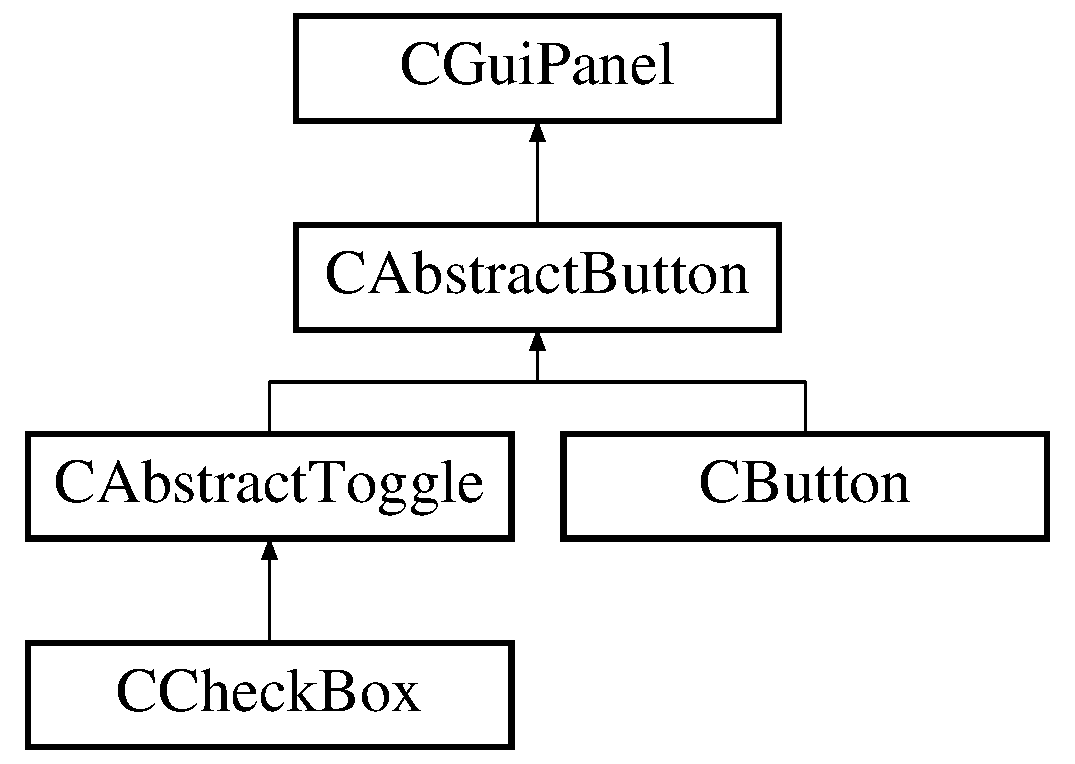
\includegraphics[height=4.000000cm]{class_c_abstract_button}
\end{center}
\end{figure}
\subsection*{Public Member Functions}
\begin{DoxyCompactItemize}
\item 
\hypertarget{class_c_abstract_button_aebe8da66b17839a626d25676210e366f}{
{\bfseries CAbstractButton} (const \hyperlink{classvec2d}{vec2d} \&pos, const \hyperlink{classvec2d}{vec2d} \&size)}
\label{class_c_abstract_button_aebe8da66b17839a626d25676210e366f}

\item 
\hypertarget{class_c_abstract_button_a48dfc32c5c3dc4012559b55240bcbcfd}{
virtual void {\bfseries onMouseDown} (const \hyperlink{classvec2d}{vec2d} \&position, const MouseButton button)}
\label{class_c_abstract_button_a48dfc32c5c3dc4012559b55240bcbcfd}

\item 
\hypertarget{class_c_abstract_button_a71cb204ddfd7d678aca1ba18721acbf8}{
virtual void {\bfseries onMouseUp} (const \hyperlink{classvec2d}{vec2d} \&position, const MouseButton button)}
\label{class_c_abstract_button_a71cb204ddfd7d678aca1ba18721acbf8}

\item 
\hypertarget{class_c_abstract_button_a439458155d8e3283adb9ea62ee48c7f2}{
virtual void {\bfseries onMouseOver} ()}
\label{class_c_abstract_button_a439458155d8e3283adb9ea62ee48c7f2}

\item 
\hypertarget{class_c_abstract_button_ac61d5051600b09c9f5d9a93cb5211562}{
virtual void {\bfseries onMouseOut} ()}
\label{class_c_abstract_button_ac61d5051600b09c9f5d9a93cb5211562}

\end{DoxyCompactItemize}
\subsection*{Protected Attributes}
\begin{DoxyCompactItemize}
\item 
\hypertarget{class_c_abstract_button_a75207c5f3b0bbbacbcde194ec6db61e8}{
bool {\bfseries \_\-active}}
\label{class_c_abstract_button_a75207c5f3b0bbbacbcde194ec6db61e8}

\item 
\hypertarget{class_c_abstract_button_a6a91491e0a27b9a18b5c95af38c7b0f9}{
bool {\bfseries \_\-pressed}}
\label{class_c_abstract_button_a6a91491e0a27b9a18b5c95af38c7b0f9}

\end{DoxyCompactItemize}


The documentation for this class was generated from the following files:\begin{DoxyCompactItemize}
\item 
src/gui/CAbstractButton.h\item 
src/gui/CAbstractButton.cpp\end{DoxyCompactItemize}

\hypertarget{class_c_abstract_toggle}{
\section{CAbstractToggle Class Reference}
\label{class_c_abstract_toggle}\index{CAbstractToggle@{CAbstractToggle}}
}
Inheritance diagram for CAbstractToggle:\begin{figure}[H]
\begin{center}
\leavevmode
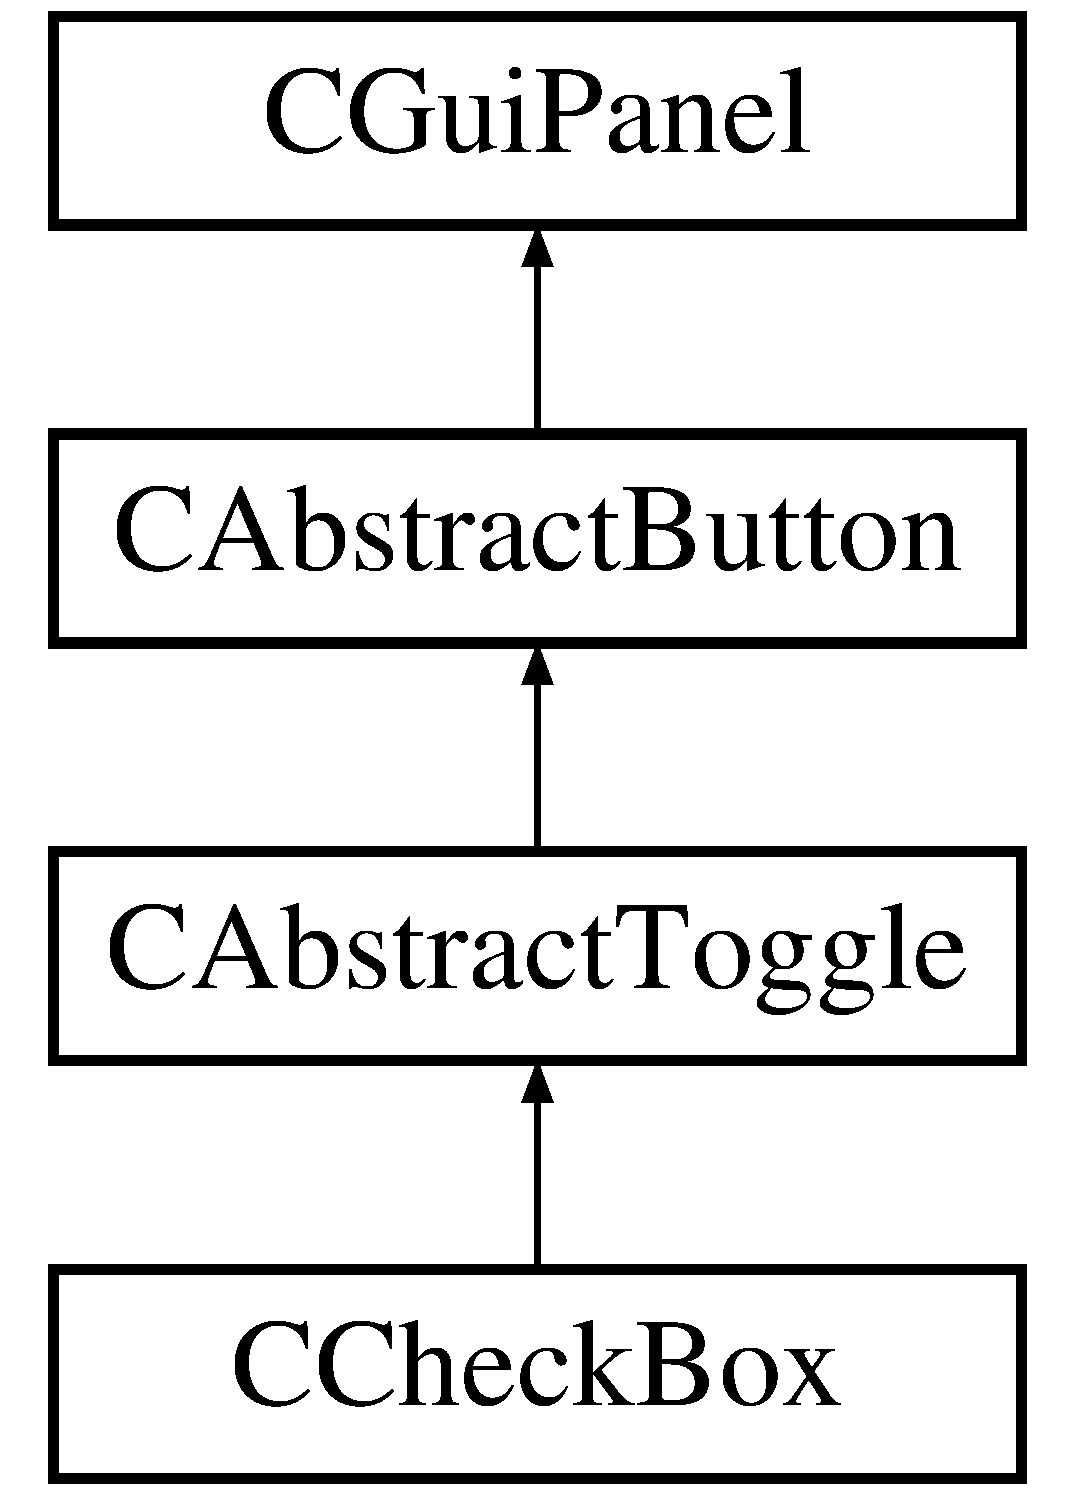
\includegraphics[height=4.000000cm]{class_c_abstract_toggle}
\end{center}
\end{figure}
\subsection*{Public Member Functions}
\begin{DoxyCompactItemize}
\item 
\hypertarget{class_c_abstract_toggle_a57b1c9d62c8cc6e53b483afb2d329b16}{
{\bfseries CAbstractToggle} (const \hyperlink{classvec2d}{vec2d} \&pos, const \hyperlink{classvec2d}{vec2d} \&size, bool selected=false)}
\label{class_c_abstract_toggle_a57b1c9d62c8cc6e53b483afb2d329b16}

\item 
\hypertarget{class_c_abstract_toggle_a0cef5f815d59738647bf1d3ae130ee75}{
{\bfseries CAbstractToggle} (const \hyperlink{classvec2d}{vec2d} \&pos, const \hyperlink{classvec2d}{vec2d} \&size)}
\label{class_c_abstract_toggle_a0cef5f815d59738647bf1d3ae130ee75}

\item 
\hypertarget{class_c_abstract_toggle_ad96f8f6e17fdbb72e2c76358496f395e}{
bool {\bfseries getSelected} ()}
\label{class_c_abstract_toggle_ad96f8f6e17fdbb72e2c76358496f395e}

\item 
\hypertarget{class_c_abstract_toggle_adf89a794ba7ad5af46d6a65adadcb727}{
virtual void {\bfseries onStateChanged} ()=0}
\label{class_c_abstract_toggle_adf89a794ba7ad5af46d6a65adadcb727}

\item 
\hypertarget{class_c_abstract_toggle_a43c338306fc3661aa217716047b424ad}{
virtual void {\bfseries onMouseClick} (const \hyperlink{classvec2d}{vec2d} \&position, const MouseButton button)}
\label{class_c_abstract_toggle_a43c338306fc3661aa217716047b424ad}

\end{DoxyCompactItemize}
\subsection*{Protected Attributes}
\begin{DoxyCompactItemize}
\item 
\hypertarget{class_c_abstract_toggle_a842605c85e31e1094ef358de17601585}{
bool {\bfseries \_\-selected}}
\label{class_c_abstract_toggle_a842605c85e31e1094ef358de17601585}

\end{DoxyCompactItemize}


The documentation for this class was generated from the following files:\begin{DoxyCompactItemize}
\item 
src/gui/CAbstractToggle.h\item 
src/gui/CAbstractToggle.cpp\end{DoxyCompactItemize}

\hypertarget{class_c_action_listener}{
\section{CActionListener Class Reference}
\label{class_c_action_listener}\index{CActionListener@{CActionListener}}
}
\subsection*{Public Member Functions}
\begin{DoxyCompactItemize}
\item 
\hypertarget{class_c_action_listener_ab8acd0c528a02e67c99b18ed86766160}{
{\bfseries CActionListener} (\hyperlink{class_c_action_listener_panel}{CActionListenerPanel} $\ast$panel, int id)}
\label{class_c_action_listener_ab8acd0c528a02e67c99b18ed86766160}

\item 
\hypertarget{class_c_action_listener_a933066180a2fde943e51958589248d5c}{
int {\bfseries getId} ()}
\label{class_c_action_listener_a933066180a2fde943e51958589248d5c}

\item 
\hypertarget{class_c_action_listener_a3418ba195f34df54d13e6a3d9bdd8fb4}{
void {\bfseries setOriginator} (\hyperlink{class_c_gui_panel}{CGuiPanel} $\ast$originator)}
\label{class_c_action_listener_a3418ba195f34df54d13e6a3d9bdd8fb4}

\item 
\hypertarget{class_c_action_listener_ae515ec689cd0f428c2c306210d075c8e}{
\hyperlink{class_c_gui_panel}{CGuiPanel} $\ast$ {\bfseries getOriginator} ()}
\label{class_c_action_listener_ae515ec689cd0f428c2c306210d075c8e}

\item 
\hypertarget{class_c_action_listener_a00298af5a1be8beaeb4bb88835832922}{
virtual void {\bfseries actionPerformed} ()}
\label{class_c_action_listener_a00298af5a1be8beaeb4bb88835832922}

\end{DoxyCompactItemize}


The documentation for this class was generated from the following file:\begin{DoxyCompactItemize}
\item 
src/gui/CActionListener.h\end{DoxyCompactItemize}

\hypertarget{class_c_action_listener_panel}{
\section{CActionListenerPanel Class Reference}
\label{class_c_action_listener_panel}\index{CActionListenerPanel@{CActionListenerPanel}}
}
Inheritance diagram for CActionListenerPanel:\begin{figure}[H]
\begin{center}
\leavevmode
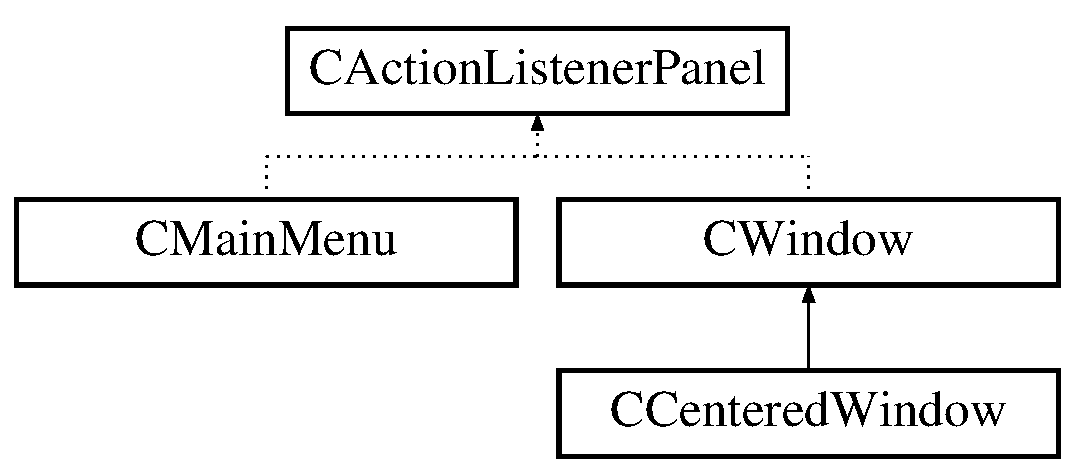
\includegraphics[height=3.000000cm]{class_c_action_listener_panel}
\end{center}
\end{figure}
\subsection*{Public Member Functions}
\begin{DoxyCompactItemize}
\item 
\hypertarget{class_c_action_listener_panel_a95c59d1d1735c5312ffdffbb8c901281}{
virtual void {\bfseries actionPerformed} (int id)=0}
\label{class_c_action_listener_panel_a95c59d1d1735c5312ffdffbb8c901281}

\end{DoxyCompactItemize}


The documentation for this class was generated from the following file:\begin{DoxyCompactItemize}
\item 
src/gui/CActionListenerPanel.h\end{DoxyCompactItemize}

\hypertarget{class_c_base_engine}{
\section{CBaseEngine Class Reference}
\label{class_c_base_engine}\index{CBaseEngine@{CBaseEngine}}
}
\subsection*{Public Member Functions}
\begin{DoxyCompactItemize}
\item 
\hypertarget{class_c_base_engine_a9317cc0ea0ea95db977d4007c1cdc79a}{
void {\bfseries init} ()}
\label{class_c_base_engine_a9317cc0ea0ea95db977d4007c1cdc79a}

\item 
\hypertarget{class_c_base_engine_a876301de40f6e8f46cb575c78a14edfb}{
void {\bfseries destroy} ()}
\label{class_c_base_engine_a876301de40f6e8f46cb575c78a14edfb}

\item 
\hypertarget{class_c_base_engine_a64de0ea7d950b86c6128b7a599c93554}{
void {\bfseries setDrawPos} (double x, double y, double z)}
\label{class_c_base_engine_a64de0ea7d950b86c6128b7a599c93554}

\item 
\hypertarget{class_c_base_engine_af1e4044b6331cf52c553ef3ab378a066}{
void {\bfseries setDrawPos} (\hyperlink{classvec3d}{vec3d} pos)}
\label{class_c_base_engine_af1e4044b6331cf52c553ef3ab378a066}

\item 
\hypertarget{class_c_base_engine_a34636846e1aaa5d12a279c3c333da20f}{
void {\bfseries setDrawColor} (float r, float g, float b, float a)}
\label{class_c_base_engine_a34636846e1aaa5d12a279c3c333da20f}

\item 
\hypertarget{class_c_base_engine_a8ccf173fea0679fd1d5044a5d871f23f}{
void {\bfseries setDrawColor} (\hyperlink{classrgba}{rgba} col)}
\label{class_c_base_engine_a8ccf173fea0679fd1d5044a5d871f23f}

\item 
\hypertarget{class_c_base_engine_aabc5cdf56e652abd70c239464cfca056}{
void {\bfseries drawModel} (int wmId)}
\label{class_c_base_engine_aabc5cdf56e652abd70c239464cfca056}

\item 
\hypertarget{class_c_base_engine_ab16ca91a8828127cb4523069d771236c}{
double {\bfseries getTime} () const }
\label{class_c_base_engine_ab16ca91a8828127cb4523069d771236c}

\item 
\hypertarget{class_c_base_engine_a7a128539bc09b8dbc219fec3b5d09f04}{
double {\bfseries getLastTime} () const }
\label{class_c_base_engine_a7a128539bc09b8dbc219fec3b5d09f04}

\item 
\hypertarget{class_c_base_engine_a639af0fb7070b46c3caf532572ebd3bf}{
double {\bfseries getTimeDelta} () const }
\label{class_c_base_engine_a639af0fb7070b46c3caf532572ebd3bf}

\item 
\hypertarget{class_c_base_engine_aec8538dfc4c28b195c4cefbceff373ff}{
double {\bfseries getRealTime} () const }
\label{class_c_base_engine_aec8538dfc4c28b195c4cefbceff373ff}

\item 
\hypertarget{class_c_base_engine_aee4bfbcd8f699c89a0f1ce96abd8e822}{
double {\bfseries getLastRealTime} () const }
\label{class_c_base_engine_aee4bfbcd8f699c89a0f1ce96abd8e822}

\item 
\hypertarget{class_c_base_engine_ac1a7b9f07d661fe7ef6bbdc98e553525}{
double {\bfseries getRealTimeDelta} () const }
\label{class_c_base_engine_ac1a7b9f07d661fe7ef6bbdc98e553525}

\item 
\hypertarget{class_c_base_engine_abd49d564d1aecd528039897b21eef66a}{
unsigned long long int {\bfseries getFrameCount} () const }
\label{class_c_base_engine_abd49d564d1aecd528039897b21eef66a}

\item 
\hypertarget{class_c_base_engine_adce5f957133b5e2b7ccca631355800ad}{
double {\bfseries getFPS} () const }
\label{class_c_base_engine_adce5f957133b5e2b7ccca631355800ad}

\item 
\hypertarget{class_c_base_engine_a70f80b67ea65db4fb56b1a86acdacdfc}{
void {\bfseries createEntity} (std::string name)}
\label{class_c_base_engine_a70f80b67ea65db4fb56b1a86acdacdfc}

\item 
\hypertarget{class_c_base_engine_a044ac7781508da2aa24bf74cd2b36d7f}{
void {\bfseries think} ()}
\label{class_c_base_engine_a044ac7781508da2aa24bf74cd2b36d7f}

\item 
\hypertarget{class_c_base_engine_af56586ffe12fc017e75b9104bde5398d}{
void {\bfseries initWorldView} ()}
\label{class_c_base_engine_af56586ffe12fc017e75b9104bde5398d}

\item 
\hypertarget{class_c_base_engine_a87e5248572323ef5847361177122ffcf}{
void {\bfseries initGuiView} ()}
\label{class_c_base_engine_a87e5248572323ef5847361177122ffcf}

\item 
\hypertarget{class_c_base_engine_adcff4ed3343e6e5ebd0d68c0945f72c7}{
void {\bfseries drawScene} ()}
\label{class_c_base_engine_adcff4ed3343e6e5ebd0d68c0945f72c7}

\item 
\hypertarget{class_c_base_engine_a58b7fcf0e4ab9d4a1bbc78d30af5d842}{
void {\bfseries log} (const std::wstring \&text)}
\label{class_c_base_engine_a58b7fcf0e4ab9d4a1bbc78d30af5d842}

\item 
\hypertarget{class_c_base_engine_a321c2e7107401c9d79277fa49bd28453}{
void {\bfseries quit} ()}
\label{class_c_base_engine_a321c2e7107401c9d79277fa49bd28453}

\end{DoxyCompactItemize}
\subsection*{Public Attributes}
\begin{DoxyCompactItemize}
\item 
\hypertarget{class_c_base_engine_a7bcd6139db14be811a9c5a70eeb8ef82}{
\hyperlink{class_c_ent_mgr}{CEntMgr} $\ast$ {\bfseries ents}}
\label{class_c_base_engine_a7bcd6139db14be811a9c5a70eeb8ef82}

\item 
\hypertarget{class_c_base_engine_afd4d462278f92d88035c1709f707b341}{
\hyperlink{class_c_input_mgr}{CInputMgr} $\ast$ {\bfseries input}}
\label{class_c_base_engine_afd4d462278f92d88035c1709f707b341}

\item 
\hypertarget{class_c_base_engine_a4d6c213d3f468f0248440bc69a4eb43b}{
\hyperlink{class_c_gui_mgr}{CGuiMgr} $\ast$ {\bfseries gui}}
\label{class_c_base_engine_a4d6c213d3f468f0248440bc69a4eb43b}

\item 
\hypertarget{class_c_base_engine_a4dab7710b5d4e16f44ff35059479ce46}{
\hyperlink{class_c_font_mgr}{CFontMgr} $\ast$ {\bfseries fonts}}
\label{class_c_base_engine_a4dab7710b5d4e16f44ff35059479ce46}

\item 
\hypertarget{class_c_base_engine_a24d401bf5313cb353c631ed179eaf48f}{
\hyperlink{class_font}{Font} $\ast$ {\bfseries systemFont}}
\label{class_c_base_engine_a24d401bf5313cb353c631ed179eaf48f}

\end{DoxyCompactItemize}


The documentation for this class was generated from the following files:\begin{DoxyCompactItemize}
\item 
src/CBaseEngine.h\item 
src/CBaseEngine.cpp\end{DoxyCompactItemize}

\hypertarget{class_c_base_entity}{
\section{CBaseEntity Class Reference}
\label{class_c_base_entity}\index{CBaseEntity@{CBaseEntity}}
}
\subsection*{Public Member Functions}
\begin{DoxyCompactItemize}
\item 
\hypertarget{class_c_base_entity_ac48b4dc380ceebcc66d4243227732430}{
virtual void {\bfseries init} ()}
\label{class_c_base_entity_ac48b4dc380ceebcc66d4243227732430}

\item 
\hypertarget{class_c_base_entity_acdf031fbf15e1afb0d5365a14f4cae34}{
virtual void {\bfseries think} ()}
\label{class_c_base_entity_acdf031fbf15e1afb0d5365a14f4cae34}

\item 
\hypertarget{class_c_base_entity_a9877f7539c282bfe7ee02a6cd29382e9}{
virtual void {\bfseries draw} ()}
\label{class_c_base_entity_a9877f7539c282bfe7ee02a6cd29382e9}

\item 
\hypertarget{class_c_base_entity_aef5bc8ccedc1b36e2fbcd7fcb0361175}{
virtual void {\bfseries processCollision} (\hyperlink{class_c_base_entity}{CBaseEntity} $\ast$collider)}
\label{class_c_base_entity_aef5bc8ccedc1b36e2fbcd7fcb0361175}

\item 
\hypertarget{class_c_base_entity_a0557e8188cb9529da164d5ae0e63c41c}{
virtual \hyperlink{classvec3d}{vec3d} {\bfseries getPos} ()}
\label{class_c_base_entity_a0557e8188cb9529da164d5ae0e63c41c}

\end{DoxyCompactItemize}
\subsection*{Public Attributes}
\begin{DoxyCompactItemize}
\item 
\hypertarget{class_c_base_entity_acc7a3833bb1ed7064713d52ce70e3119}{
\hyperlink{class_c_param_mgr}{CParamMgr} {\bfseries params}}
\label{class_c_base_entity_acc7a3833bb1ed7064713d52ce70e3119}

\end{DoxyCompactItemize}


The documentation for this class was generated from the following files:\begin{DoxyCompactItemize}
\item 
src/CBaseEntity.h\item 
src/CBaseEntity.cpp\end{DoxyCompactItemize}

\hypertarget{class_c_button}{
\section{CButton Class Reference}
\label{class_c_button}\index{CButton@{CButton}}
}
Inheritance diagram for CButton:\begin{figure}[H]
\begin{center}
\leavevmode
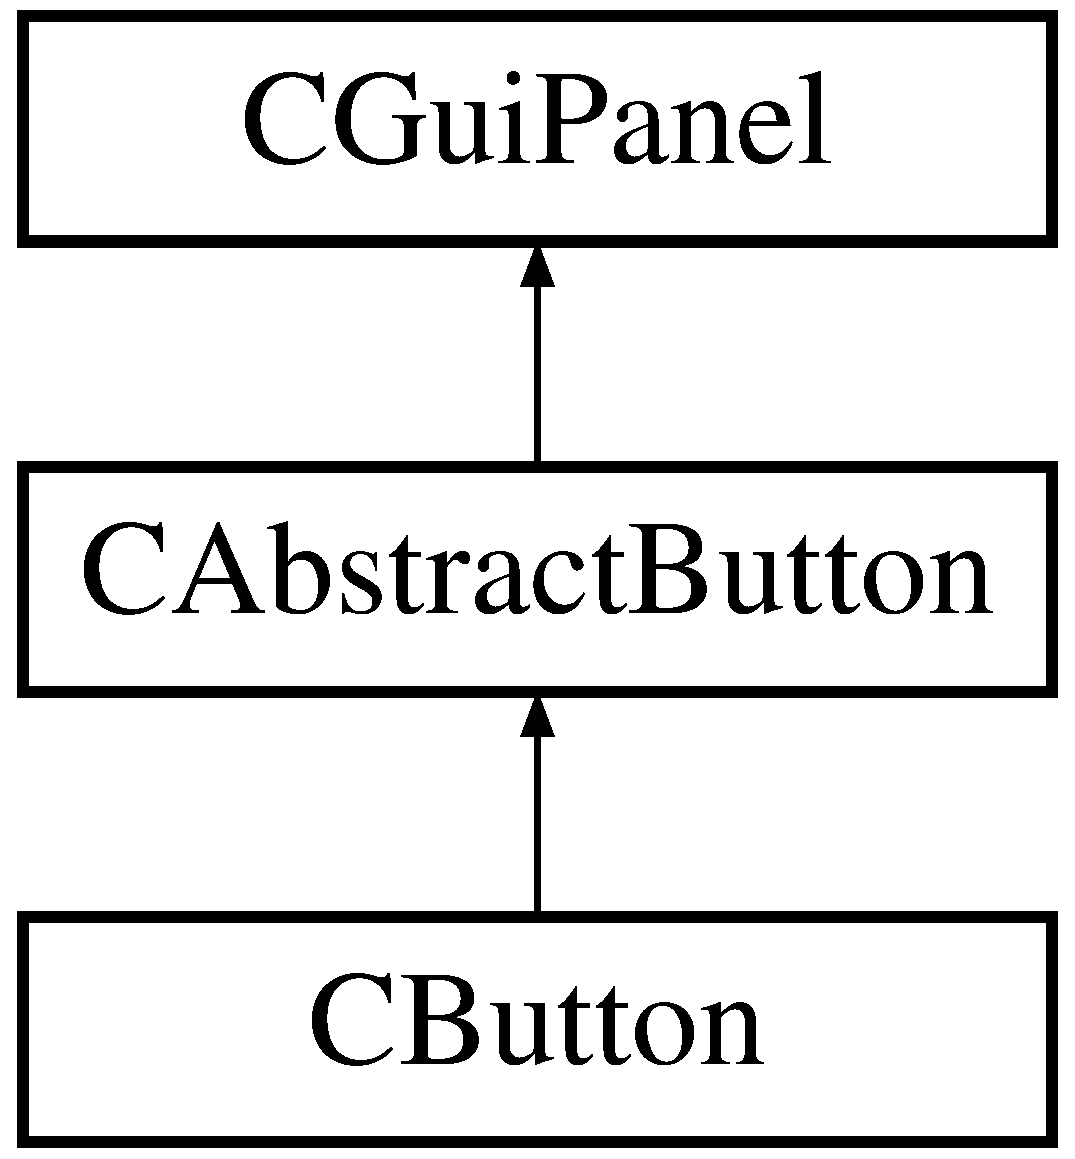
\includegraphics[height=3.000000cm]{class_c_button}
\end{center}
\end{figure}
\subsection*{Public Member Functions}
\begin{DoxyCompactItemize}
\item 
\hypertarget{class_c_button_a817841919e8ed28c21edde93768ba56d}{
{\bfseries CButton} (const \hyperlink{classvec2d}{vec2d} \&pos, const \hyperlink{classvec2d}{vec2d} \&size, const std::wstring \&text)}
\label{class_c_button_a817841919e8ed28c21edde93768ba56d}

\item 
\hypertarget{class_c_button_abf2c2a6bb002631bbe2c6dde5d73925b}{
virtual void {\bfseries draw} ()}
\label{class_c_button_abf2c2a6bb002631bbe2c6dde5d73925b}

\item 
\hypertarget{class_c_button_a03b5374e6d90fea0d6ede8d6a0fbd1a3}{
virtual void {\bfseries onMouseClick} (const \hyperlink{classvec2d}{vec2d} \&position, const MouseButton button)}
\label{class_c_button_a03b5374e6d90fea0d6ede8d6a0fbd1a3}

\end{DoxyCompactItemize}
\subsection*{Protected Attributes}
\begin{DoxyCompactItemize}
\item 
\hypertarget{class_c_button_a7641ebdd3f3c68ae593cc12069f80a7c}{
\hyperlink{class_c_label}{CLabel} $\ast$ {\bfseries label}}
\label{class_c_button_a7641ebdd3f3c68ae593cc12069f80a7c}

\item 
\hypertarget{class_c_button_a8de5eb1d2eb624ec5138d63badc7a87f}{
\hyperlink{classrgba}{rgba} {\bfseries bgTopColor}}
\label{class_c_button_a8de5eb1d2eb624ec5138d63badc7a87f}

\end{DoxyCompactItemize}


The documentation for this class was generated from the following files:\begin{DoxyCompactItemize}
\item 
src/gui/CButton.h\item 
src/gui/CButton.cpp\end{DoxyCompactItemize}

\hypertarget{class_c_centered_window}{
\section{CCenteredWindow Class Reference}
\label{class_c_centered_window}\index{CCenteredWindow@{CCenteredWindow}}
}
Inheritance diagram for CCenteredWindow:\begin{figure}[H]
\begin{center}
\leavevmode
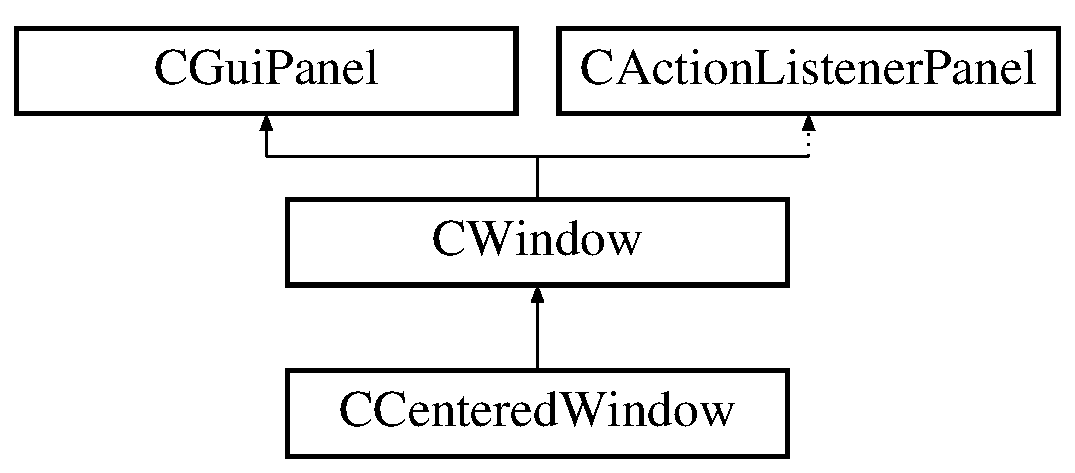
\includegraphics[height=3.000000cm]{class_c_centered_window}
\end{center}
\end{figure}
\subsection*{Public Member Functions}
\begin{DoxyCompactItemize}
\item 
\hypertarget{class_c_centered_window_ade79256083d0fdeff7422d922f44cd13}{
{\bfseries CCenteredWindow} (const \hyperlink{classvec2d}{vec2d} \&size, const std::wstring \&label)}
\label{class_c_centered_window_ade79256083d0fdeff7422d922f44cd13}

\end{DoxyCompactItemize}


The documentation for this class was generated from the following files:\begin{DoxyCompactItemize}
\item 
src/gui/CCenteredWindow.h\item 
src/gui/CCenteredWindow.cpp\end{DoxyCompactItemize}

\hypertarget{class_c_check_box}{
\section{CCheckBox Class Reference}
\label{class_c_check_box}\index{CCheckBox@{CCheckBox}}
}
Inheritance diagram for CCheckBox:\begin{figure}[H]
\begin{center}
\leavevmode
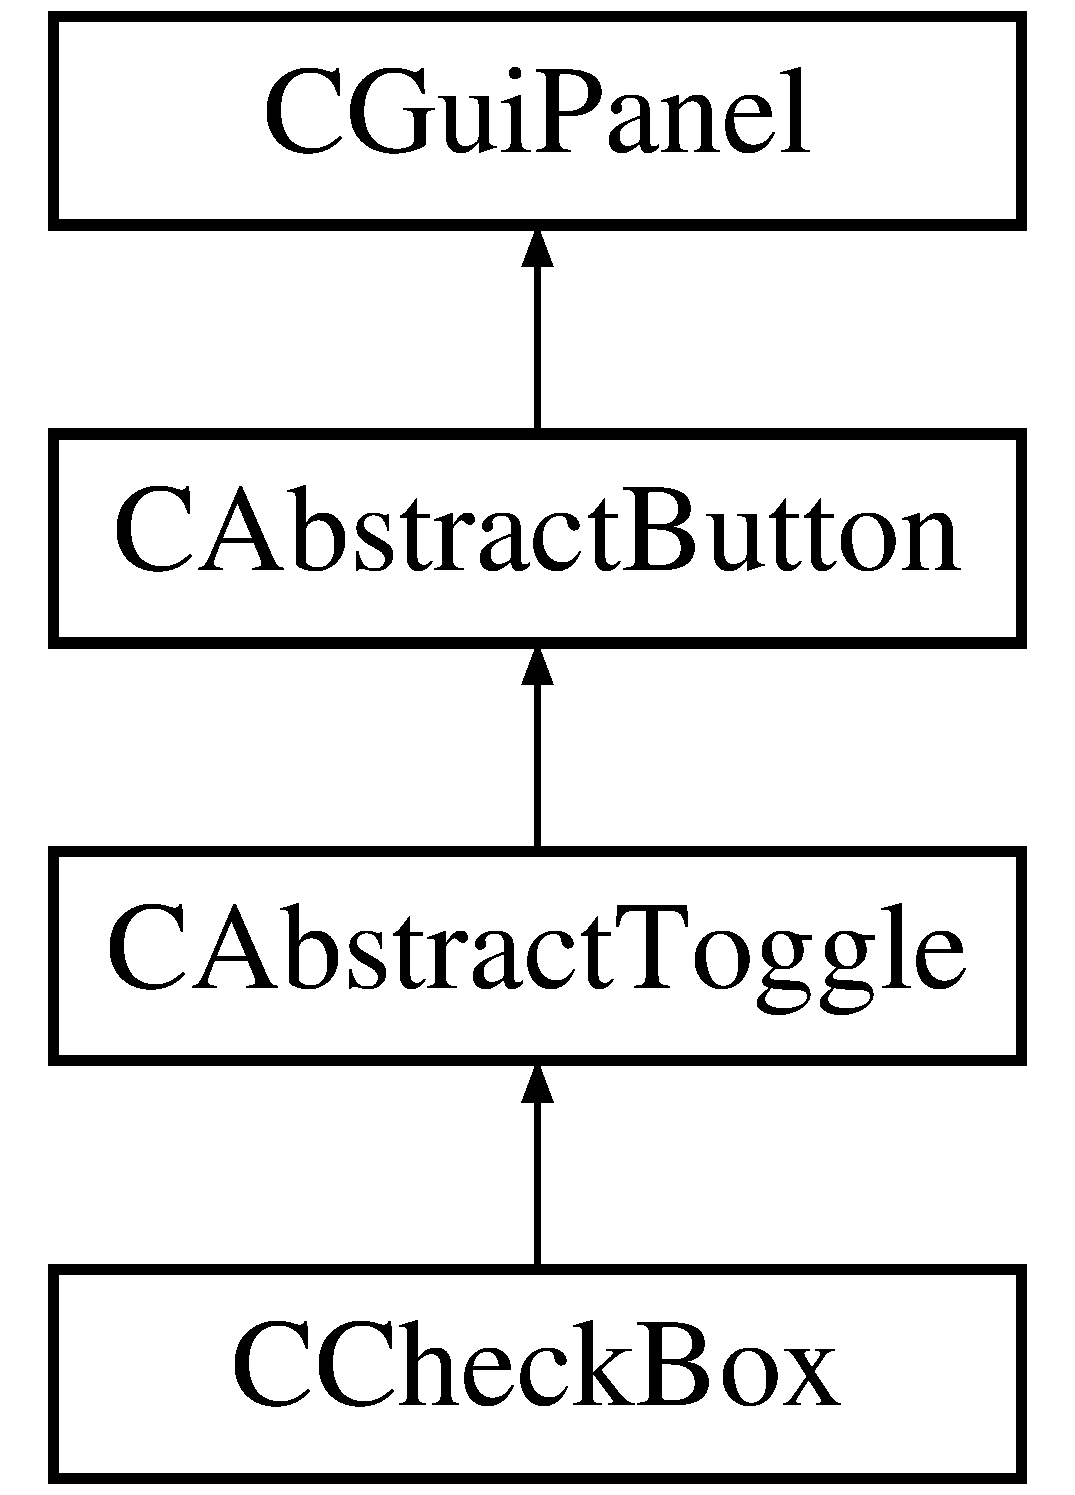
\includegraphics[height=4.000000cm]{class_c_check_box}
\end{center}
\end{figure}
\subsection*{Public Member Functions}
\begin{DoxyCompactItemize}
\item 
\hypertarget{class_c_check_box_a21990bd8234ba49ca8f33ef23635e069}{
{\bfseries CCheckBox} (const \hyperlink{classvec2d}{vec2d} \&pos, const \hyperlink{classvec2d}{vec2d} \&size, const std::wstring \&text, bool selected=false)}
\label{class_c_check_box_a21990bd8234ba49ca8f33ef23635e069}

\item 
\hypertarget{class_c_check_box_a2352dc124cd865d4abdcc04e2a1c2a16}{
virtual void {\bfseries draw} ()}
\label{class_c_check_box_a2352dc124cd865d4abdcc04e2a1c2a16}

\item 
\hypertarget{class_c_check_box_a5b948b67b82f9db41249edb2201fa98a}{
virtual void {\bfseries onStateChanged} ()}
\label{class_c_check_box_a5b948b67b82f9db41249edb2201fa98a}

\end{DoxyCompactItemize}


The documentation for this class was generated from the following files:\begin{DoxyCompactItemize}
\item 
src/gui/CCheckBox.h\item 
src/gui/CCheckBox.cpp\end{DoxyCompactItemize}

\hypertarget{class_c_draggable}{
\section{CDraggable Class Reference}
\label{class_c_draggable}\index{CDraggable@{CDraggable}}
}
Inheritance diagram for CDraggable:\begin{figure}[H]
\begin{center}
\leavevmode
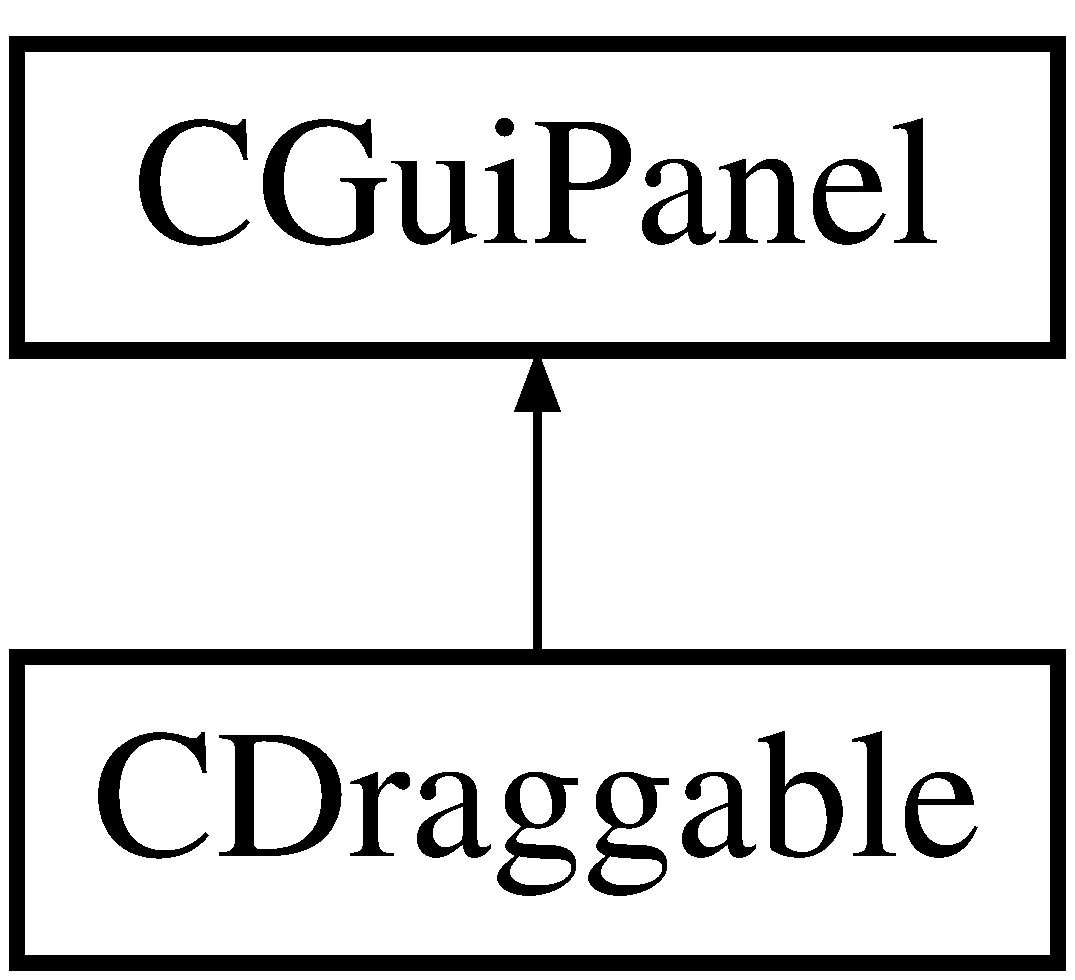
\includegraphics[height=2.000000cm]{class_c_draggable}
\end{center}
\end{figure}
\subsection*{Public Member Functions}
\begin{DoxyCompactItemize}
\item 
\hypertarget{class_c_draggable_aff479e1e062a04dc3cf4707f01df1226}{
{\bfseries CDraggable} (const \hyperlink{classvec2d}{vec2d} \&position, const \hyperlink{classvec2d}{vec2d} \&size)}
\label{class_c_draggable_aff479e1e062a04dc3cf4707f01df1226}

\item 
\hypertarget{class_c_draggable_ad8345786e317adf5100c324bfc9c4642}{
virtual void {\bfseries mouseMove} (const \hyperlink{classvec2d}{vec2d} \&newPosition, const bool mouseOver)}
\label{class_c_draggable_ad8345786e317adf5100c324bfc9c4642}

\item 
\hypertarget{class_c_draggable_a11be111cac73c2118049921ad532a42b}{
virtual void {\bfseries onMouseDown} (const \hyperlink{classvec2d}{vec2d} \&position, const MouseButton button)}
\label{class_c_draggable_a11be111cac73c2118049921ad532a42b}

\item 
\hypertarget{class_c_draggable_aea986fad441b728234d7892307ae9a7a}{
virtual void {\bfseries onMouseUp} (const \hyperlink{classvec2d}{vec2d} \&position, const MouseButton button)}
\label{class_c_draggable_aea986fad441b728234d7892307ae9a7a}

\item 
\hypertarget{class_c_draggable_aaac9d4d4827aea7fb8e63c3f1413a752}{
virtual void {\bfseries draw} ()}
\label{class_c_draggable_aaac9d4d4827aea7fb8e63c3f1413a752}

\end{DoxyCompactItemize}
\subsection*{Protected Attributes}
\begin{DoxyCompactItemize}
\item 
\hypertarget{class_c_draggable_a3caac7d16cd002330368b43439e22e6c}{
\hyperlink{classvec2d}{vec2d} {\bfseries lastPosition}}
\label{class_c_draggable_a3caac7d16cd002330368b43439e22e6c}

\item 
\hypertarget{class_c_draggable_ab48356d215bf3572f87465a7205f048e}{
bool {\bfseries pressed}}
\label{class_c_draggable_ab48356d215bf3572f87465a7205f048e}

\end{DoxyCompactItemize}


The documentation for this class was generated from the following files:\begin{DoxyCompactItemize}
\item 
src/gui/CDraggable.h\item 
src/gui/CDraggable.cpp\end{DoxyCompactItemize}

\hypertarget{class_c_ent_mgr}{
\section{CEntMgr Class Reference}
\label{class_c_ent_mgr}\index{CEntMgr@{CEntMgr}}
}
\subsection*{Public Member Functions}
\begin{DoxyCompactItemize}
\item 
\hypertarget{class_c_ent_mgr_a623eb404662b2bcf74d9d4ebe6fd3021}{
int {\bfseries getEntCount} ()}
\label{class_c_ent_mgr_a623eb404662b2bcf74d9d4ebe6fd3021}

\item 
\hypertarget{class_c_ent_mgr_ada1f34090a70b3949e7f1bd9223d55c6}{
\hyperlink{class_c_base_entity}{CBaseEntity} $\ast$ {\bfseries getEntById} (int id)}
\label{class_c_ent_mgr_ada1f34090a70b3949e7f1bd9223d55c6}

\item 
\hypertarget{class_c_ent_mgr_a1b3ad334624feb388cbec543511ab498}{
int {\bfseries getEntCountByTargetName} (std::string targetname)}
\label{class_c_ent_mgr_a1b3ad334624feb388cbec543511ab498}

\item 
\hypertarget{class_c_ent_mgr_a98baf0e2b6889816a5414ae98b429884}{
void {\bfseries findEntsByTargetName} (std::string targetname)}
\label{class_c_ent_mgr_a98baf0e2b6889816a5414ae98b429884}

\item 
\hypertarget{class_c_ent_mgr_ab6a9fa88afc9f47a0207bd67494866d7}{
void {\bfseries findEntsInSphere} (\hyperlink{classvec3d}{vec3d} pos, double radius)}
\label{class_c_ent_mgr_ab6a9fa88afc9f47a0207bd67494866d7}

\item 
\hypertarget{class_c_ent_mgr_a980881fc39db9e17f7d369fc26643e61}{
\hyperlink{class_c_base_entity}{CBaseEntity} $\ast$ {\bfseries getNextEntFromLastSearch} ()}
\label{class_c_ent_mgr_a980881fc39db9e17f7d369fc26643e61}

\end{DoxyCompactItemize}


The documentation for this class was generated from the following files:\begin{DoxyCompactItemize}
\item 
src/CEntMgr.h\item 
src/CEntMgr.cpp\end{DoxyCompactItemize}

\hypertarget{class_c_font_mgr}{
\section{CFontMgr Class Reference}
\label{class_c_font_mgr}\index{CFontMgr@{CFontMgr}}
}
\subsection*{Public Member Functions}
\begin{DoxyCompactItemize}
\item 
\hypertarget{class_c_font_mgr_a9c467342ba57f52015d52c10b2da1b04}{
\hyperlink{class_font}{Font} $\ast$ {\bfseries getFont} (const wstring \&name)}
\label{class_c_font_mgr_a9c467342ba57f52015d52c10b2da1b04}

\item 
\hypertarget{class_c_font_mgr_a9a03a0f0cf8fc24d0ac9b2764b7cec4c}{
\hyperlink{class_font}{Font} $\ast$ {\bfseries loadFont} (const wstring \&name, const double size)}
\label{class_c_font_mgr_a9a03a0f0cf8fc24d0ac9b2764b7cec4c}

\end{DoxyCompactItemize}


The documentation for this class was generated from the following files:\begin{DoxyCompactItemize}
\item 
src/CFontMgr.h\item 
src/CFontMgr.cpp\end{DoxyCompactItemize}

\hypertarget{class_c_gui_mgr}{
\section{CGuiMgr Class Reference}
\label{class_c_gui_mgr}\index{CGuiMgr@{CGuiMgr}}
}
\subsection*{Public Member Functions}
\begin{DoxyCompactItemize}
\item 
\hypertarget{class_c_gui_mgr_a67a77bf82141c990553ca4ea27144800}{
void {\bfseries init} ()}
\label{class_c_gui_mgr_a67a77bf82141c990553ca4ea27144800}

\item 
\hypertarget{class_c_gui_mgr_ab8f078d06299736a552fa25ea52aba6d}{
void {\bfseries update} ()}
\label{class_c_gui_mgr_ab8f078d06299736a552fa25ea52aba6d}

\item 
\hypertarget{class_c_gui_mgr_a745c61a4ed47b24ec10d404e6603ca7f}{
void {\bfseries drawElements} ()}
\label{class_c_gui_mgr_a745c61a4ed47b24ec10d404e6603ca7f}

\item 
\hypertarget{class_c_gui_mgr_a0b791d7ac971fded45ac14cbffa24840}{
void {\bfseries setKeyboardReceiver} (\hyperlink{class_c_gui_panel}{CGuiPanel} $\ast$panel)}
\label{class_c_gui_mgr_a0b791d7ac971fded45ac14cbffa24840}

\item 
\hypertarget{class_c_gui_mgr_a38ba0aa9d04c8b95cca1145a52a1bd2c}{
bool {\bfseries isKeyboardReceiver} (\hyperlink{class_c_gui_panel}{CGuiPanel} $\ast$panel)}
\label{class_c_gui_mgr_a38ba0aa9d04c8b95cca1145a52a1bd2c}

\end{DoxyCompactItemize}
\subsection*{Public Attributes}
\begin{DoxyCompactItemize}
\item 
\hypertarget{class_c_gui_mgr_aa72d741566ce86412f2ce12081632fe5}{
\hyperlink{class_c_gui_panel}{CGuiPanel} $\ast$ {\bfseries \_\-basePanel}}
\label{class_c_gui_mgr_aa72d741566ce86412f2ce12081632fe5}

\item 
\hypertarget{class_c_gui_mgr_a39faeaa6758cb02d69df4d2308652389}{
\hyperlink{class_c_gui_panel}{CGuiPanel} $\ast$ {\bfseries \_\-keyboardReceiver}}
\label{class_c_gui_mgr_a39faeaa6758cb02d69df4d2308652389}

\end{DoxyCompactItemize}


The documentation for this class was generated from the following files:\begin{DoxyCompactItemize}
\item 
src/CGuiMgr.h\item 
src/CGuiMgr.cpp\end{DoxyCompactItemize}

\hypertarget{class_c_gui_panel}{
\section{CGuiPanel Class Reference}
\label{class_c_gui_panel}\index{CGuiPanel@{CGuiPanel}}
}
Inheritance diagram for CGuiPanel:\begin{figure}[H]
\begin{center}
\leavevmode
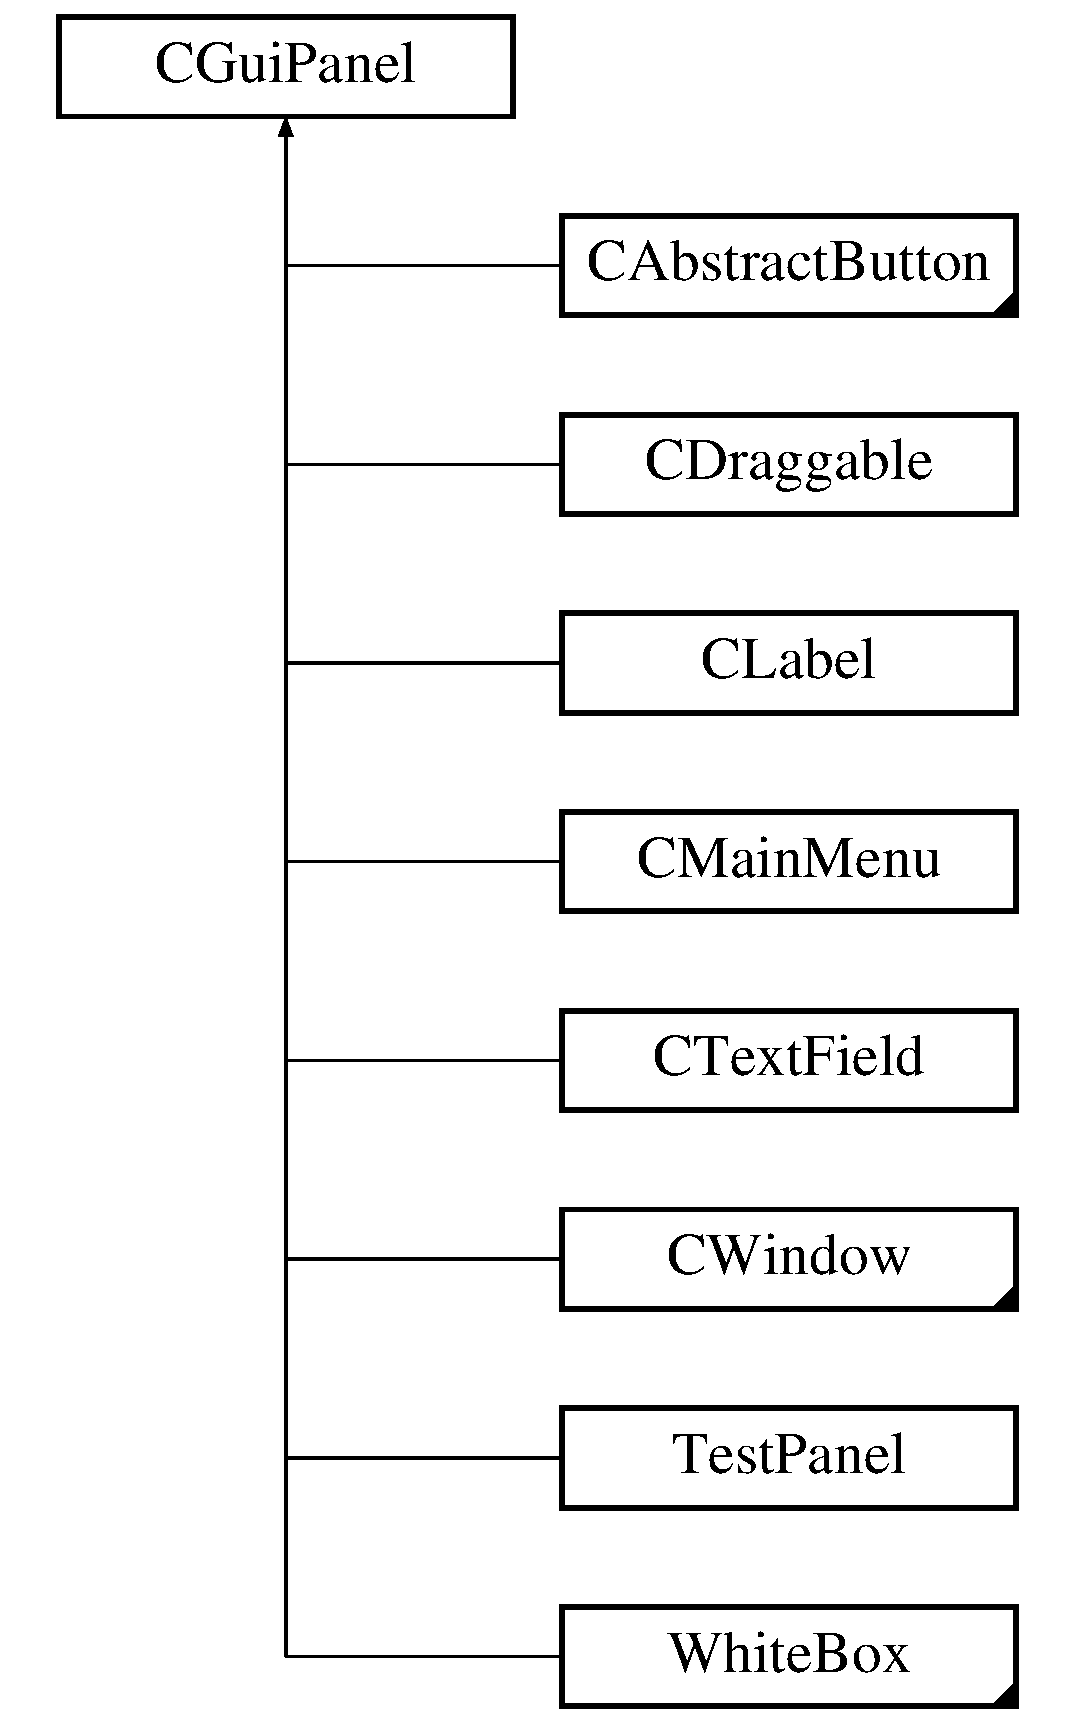
\includegraphics[height=9.000000cm]{class_c_gui_panel}
\end{center}
\end{figure}
\subsection*{Public Member Functions}
\begin{DoxyCompactItemize}
\item 
\hypertarget{class_c_gui_panel_a8110a738e143543ca3c7954793097e70}{
{\bfseries CGuiPanel} (const \hyperlink{classvec2d}{vec2d} \&pos, const \hyperlink{classvec2d}{vec2d} \&size)}
\label{class_c_gui_panel_a8110a738e143543ca3c7954793097e70}

\item 
\hypertarget{class_c_gui_panel_a3ce7a3603f1631c70f987e3d482132f4}{
void {\bfseries init} ()}
\label{class_c_gui_panel_a3ce7a3603f1631c70f987e3d482132f4}

\item 
\hypertarget{class_c_gui_panel_a33269f80691621af3072823d78d6a460}{
virtual void {\bfseries draw} ()}
\label{class_c_gui_panel_a33269f80691621af3072823d78d6a460}

\item 
\hypertarget{class_c_gui_panel_a10d81b5a153aa039e70df696c0b49780}{
virtual void {\bfseries drawChildren} ()}
\label{class_c_gui_panel_a10d81b5a153aa039e70df696c0b49780}

\item 
\hypertarget{class_c_gui_panel_a500909aeb573254a335bd62ff1898d7d}{
void {\bfseries setX} (double x)}
\label{class_c_gui_panel_a500909aeb573254a335bd62ff1898d7d}

\item 
\hypertarget{class_c_gui_panel_a4bb13f566a06d59ed13fd2b854f92fd5}{
void {\bfseries setY} (double y)}
\label{class_c_gui_panel_a4bb13f566a06d59ed13fd2b854f92fd5}

\item 
\hypertarget{class_c_gui_panel_a8aeb9a3555ea009e3c034016fca060c4}{
void {\bfseries setPosition} (double x, double y)}
\label{class_c_gui_panel_a8aeb9a3555ea009e3c034016fca060c4}

\item 
\hypertarget{class_c_gui_panel_a79f817833ef2f5a05177fe2e72f267ee}{
void {\bfseries setPosition} (\hyperlink{classvec2d}{vec2d} \&newPosition)}
\label{class_c_gui_panel_a79f817833ef2f5a05177fe2e72f267ee}

\item 
\hypertarget{class_c_gui_panel_ab171ac9172bab414f1fbb14c9e7676df}{
double {\bfseries getX} () const }
\label{class_c_gui_panel_ab171ac9172bab414f1fbb14c9e7676df}

\item 
\hypertarget{class_c_gui_panel_a9649f27f171ec883d409a140d6e92d18}{
double {\bfseries getY} () const }
\label{class_c_gui_panel_a9649f27f171ec883d409a140d6e92d18}

\item 
\hypertarget{class_c_gui_panel_a7a59458261fb94ddc653886ed7c9f0ee}{
\hyperlink{classvec2d}{vec2d} {\bfseries getPosition} () const }
\label{class_c_gui_panel_a7a59458261fb94ddc653886ed7c9f0ee}

\item 
\hypertarget{class_c_gui_panel_a99073e1362da5d946af99efa926d9c77}{
void {\bfseries setW} (double w)}
\label{class_c_gui_panel_a99073e1362da5d946af99efa926d9c77}

\item 
\hypertarget{class_c_gui_panel_a9451916191bc9ce7e119935c8c18c3e9}{
void {\bfseries setH} (double h)}
\label{class_c_gui_panel_a9451916191bc9ce7e119935c8c18c3e9}

\item 
\hypertarget{class_c_gui_panel_a37a01124bddd2b04908687862de69485}{
void {\bfseries setSize} (double w, double h)}
\label{class_c_gui_panel_a37a01124bddd2b04908687862de69485}

\item 
\hypertarget{class_c_gui_panel_aa4324d9062bd96d144155ba34c29176a}{
void {\bfseries setSize} (\hyperlink{classvec2d}{vec2d} \&newSize)}
\label{class_c_gui_panel_aa4324d9062bd96d144155ba34c29176a}

\item 
\hypertarget{class_c_gui_panel_a1f6ae8a25aeca17fe999df96422890c3}{
double {\bfseries getW} () const }
\label{class_c_gui_panel_a1f6ae8a25aeca17fe999df96422890c3}

\item 
\hypertarget{class_c_gui_panel_aeafe7467c433157b4584a692372f290d}{
double {\bfseries getH} () const }
\label{class_c_gui_panel_aeafe7467c433157b4584a692372f290d}

\item 
\hypertarget{class_c_gui_panel_aae531b29822cd2e386014d4e83621efd}{
\hyperlink{classvec2d}{vec2d} {\bfseries getSize} () const }
\label{class_c_gui_panel_aae531b29822cd2e386014d4e83621efd}

\item 
\hypertarget{class_c_gui_panel_af1c7784645d5cc3654c67d2b4a5759a6}{
virtual bool {\bfseries isPointInside} (const \hyperlink{classvec2d}{vec2d} \&point)}
\label{class_c_gui_panel_af1c7784645d5cc3654c67d2b4a5759a6}

\item 
\hypertarget{class_c_gui_panel_a657e5c19cc865a96b177d9d623961410}{
void {\bfseries setVisible} (bool vis)}
\label{class_c_gui_panel_a657e5c19cc865a96b177d9d623961410}

\item 
\hypertarget{class_c_gui_panel_af4f32f02279030741b4d779390e6438d}{
bool {\bfseries getVisible} () const }
\label{class_c_gui_panel_af4f32f02279030741b4d779390e6438d}

\item 
\hypertarget{class_c_gui_panel_a17ee16bdde22cb32a2812e5016ce4080}{
bool {\bfseries isVisible} () const }
\label{class_c_gui_panel_a17ee16bdde22cb32a2812e5016ce4080}

\item 
\hypertarget{class_c_gui_panel_a311cba7bad186311eac24f5626be4028}{
void {\bfseries setOpacity} (float opacity)}
\label{class_c_gui_panel_a311cba7bad186311eac24f5626be4028}

\item 
\hypertarget{class_c_gui_panel_a74c7bb12ba5f712a1e20c82f395feaa0}{
float {\bfseries getOpacity} () const }
\label{class_c_gui_panel_a74c7bb12ba5f712a1e20c82f395feaa0}

\item 
\hypertarget{class_c_gui_panel_a28a4009593eaf413b846785580e61b1c}{
void {\bfseries setParent} (\hyperlink{class_c_gui_panel}{CGuiPanel} $\ast$newParent)}
\label{class_c_gui_panel_a28a4009593eaf413b846785580e61b1c}

\item 
\hypertarget{class_c_gui_panel_a24be118c4d2f1838ecc56546712b5fe0}{
\hyperlink{class_c_gui_panel}{CGuiPanel} $\ast$ {\bfseries getParent} () const }
\label{class_c_gui_panel_a24be118c4d2f1838ecc56546712b5fe0}

\item 
\hypertarget{class_c_gui_panel_afb3547da8e7efd14e35ab45752a3665a}{
void {\bfseries setParentIndex} (int newParentIndex)}
\label{class_c_gui_panel_afb3547da8e7efd14e35ab45752a3665a}

\item 
\hypertarget{class_c_gui_panel_af07106a92beb040c127db814a63a87ad}{
int {\bfseries getParentIndex} () const }
\label{class_c_gui_panel_af07106a92beb040c127db814a63a87ad}

\item 
\hypertarget{class_c_gui_panel_a02c239ffbaca0a9ac53ec19030a9a670}{
void {\bfseries addChild} (\hyperlink{class_c_gui_panel}{CGuiPanel} $\ast$newChild)}
\label{class_c_gui_panel_a02c239ffbaca0a9ac53ec19030a9a670}

\item 
\hypertarget{class_c_gui_panel_a2fa0ad948093e943680322b5d84f804d}{
void {\bfseries removeChild} (\hyperlink{class_c_gui_panel}{CGuiPanel} $\ast$child)}
\label{class_c_gui_panel_a2fa0ad948093e943680322b5d84f804d}

\item 
\hypertarget{class_c_gui_panel_a431062f161b423d13770a096c080c8ad}{
void {\bfseries removeChild} (int childIndex)}
\label{class_c_gui_panel_a431062f161b423d13770a096c080c8ad}

\item 
\hypertarget{class_c_gui_panel_a65062f92bdd115bd3f813c3942c6559a}{
void {\bfseries requestFocus} ()}
\label{class_c_gui_panel_a65062f92bdd115bd3f813c3942c6559a}

\item 
\hypertarget{class_c_gui_panel_a08146fc2fbdd2dea78910fab4870ca4d}{
void {\bfseries giveFocusTo} (int childIndex)}
\label{class_c_gui_panel_a08146fc2fbdd2dea78910fab4870ca4d}

\item 
\hypertarget{class_c_gui_panel_aba1b1f8c939b6c819e5ddc959d5b4b45}{
std::string {\bfseries toString} ()}
\label{class_c_gui_panel_aba1b1f8c939b6c819e5ddc959d5b4b45}

\item 
\hypertarget{class_c_gui_panel_a194286d63943947587d46e67e55e7e52}{
virtual bool {\bfseries handleMouseClick} (const \hyperlink{classvec2d}{vec2d} \&position, const MouseButton button, const bool up)}
\label{class_c_gui_panel_a194286d63943947587d46e67e55e7e52}

\item 
\hypertarget{class_c_gui_panel_a4dd62e0da2f58fad3794fbf717643120}{
virtual void {\bfseries onMouseDown} (const \hyperlink{classvec2d}{vec2d} \&position, const MouseButton button)}
\label{class_c_gui_panel_a4dd62e0da2f58fad3794fbf717643120}

\item 
\hypertarget{class_c_gui_panel_abf7853cd073e085b4d209e046d32d1f4}{
virtual void {\bfseries onMouseUp} (const \hyperlink{classvec2d}{vec2d} \&position, const MouseButton button)}
\label{class_c_gui_panel_abf7853cd073e085b4d209e046d32d1f4}

\item 
\hypertarget{class_c_gui_panel_a09fb5f540e9177499be17f68d67d5d47}{
virtual void {\bfseries onMouseClick} (const \hyperlink{classvec2d}{vec2d} \&position, const MouseButton button)}
\label{class_c_gui_panel_a09fb5f540e9177499be17f68d67d5d47}

\item 
\hypertarget{class_c_gui_panel_a810cd53278853b92512cbbc9106c6181}{
virtual void {\bfseries handleMouseMove} (const \hyperlink{classvec2d}{vec2d} \&newPosition, const bool mouseOver)}
\label{class_c_gui_panel_a810cd53278853b92512cbbc9106c6181}

\item 
\hypertarget{class_c_gui_panel_ae3918c038c1de7215d5cb58041cb30aa}{
virtual void {\bfseries mouseMove} (const \hyperlink{classvec2d}{vec2d} \&newPosition, const bool mouseOver)}
\label{class_c_gui_panel_ae3918c038c1de7215d5cb58041cb30aa}

\item 
\hypertarget{class_c_gui_panel_a9468fcd0c26c9d1e8e78649877561ee4}{
virtual void {\bfseries onMouseOver} ()}
\label{class_c_gui_panel_a9468fcd0c26c9d1e8e78649877561ee4}

\item 
\hypertarget{class_c_gui_panel_a9da328c676294e6937691ae164fe4d30}{
virtual void {\bfseries onMouseOut} ()}
\label{class_c_gui_panel_a9da328c676294e6937691ae164fe4d30}

\item 
\hypertarget{class_c_gui_panel_a6da86076a23b5faedc9200705a6ddd80}{
bool {\bfseries getMouseOver} () const }
\label{class_c_gui_panel_a6da86076a23b5faedc9200705a6ddd80}

\item 
\hypertarget{class_c_gui_panel_afeae68f13007349fd5f7dfaa887fa5ca}{
bool {\bfseries getMouseDown} () const }
\label{class_c_gui_panel_afeae68f13007349fd5f7dfaa887fa5ca}

\item 
\hypertarget{class_c_gui_panel_a03884ea74caa603c808cbb7ea047216c}{
virtual void {\bfseries onKeyboard} (const std::wstring \&string)}
\label{class_c_gui_panel_a03884ea74caa603c808cbb7ea047216c}

\item 
\hypertarget{class_c_gui_panel_a77f7a0deca61cb708eff255bdca0c64d}{
void {\bfseries requestKeyboardFocus} ()}
\label{class_c_gui_panel_a77f7a0deca61cb708eff255bdca0c64d}

\item 
\hypertarget{class_c_gui_panel_a82fd2b377f2ddc671b77725a4ec6d5f6}{
bool {\bfseries getAllowKeyboardInput} () const }
\label{class_c_gui_panel_a82fd2b377f2ddc671b77725a4ec6d5f6}

\item 
\hypertarget{class_c_gui_panel_aa5be67893e97fdaa90dd7560552a6b9f}{
void {\bfseries addActionListener} (\hyperlink{class_c_action_listener}{CActionListener} $\ast$al)}
\label{class_c_gui_panel_aa5be67893e97fdaa90dd7560552a6b9f}

\item 
\hypertarget{class_c_gui_panel_a6b8b932df857e5f867ee0c4571f7c98c}{
void {\bfseries setBgColor} (\hyperlink{classrgba}{rgba} newBg)}
\label{class_c_gui_panel_a6b8b932df857e5f867ee0c4571f7c98c}

\item 
\hypertarget{class_c_gui_panel_a2853f62bf5fc2bdd947505b99bed9ff0}{
\hyperlink{classrgba}{rgba} {\bfseries getBgColor} () const }
\label{class_c_gui_panel_a2853f62bf5fc2bdd947505b99bed9ff0}

\item 
\hypertarget{class_c_gui_panel_adc4029bc7db20aebd2a7d0b604de7fac}{
void {\bfseries setFgColor} (\hyperlink{classrgba}{rgba} newFg)}
\label{class_c_gui_panel_adc4029bc7db20aebd2a7d0b604de7fac}

\item 
\hypertarget{class_c_gui_panel_a3b43efb863acb70f3160968990f26a55}{
\hyperlink{classrgba}{rgba} {\bfseries getFgColor} () const }
\label{class_c_gui_panel_a3b43efb863acb70f3160968990f26a55}

\item 
\hypertarget{class_c_gui_panel_ab61b8fbd2c098f78c53ca97f5f0fb016}{
void {\bfseries setDrawColor} (const \hyperlink{classrgba}{rgba} \&color)}
\label{class_c_gui_panel_ab61b8fbd2c098f78c53ca97f5f0fb016}

\item 
\hypertarget{class_c_gui_panel_a984502f3842bc694ac87d97bd790feca}{
void {\bfseries drawQuad} (float x, float y, float w, float h)}
\label{class_c_gui_panel_a984502f3842bc694ac87d97bd790feca}

\item 
\hypertarget{class_c_gui_panel_a07329837a0533a45a808065a98e7cc85}{
void {\bfseries drawVerticalGradient} (float x, float y, float w, float h, const \hyperlink{classrgba}{rgba} \&colOne, const \hyperlink{classrgba}{rgba} \&colTwo)}
\label{class_c_gui_panel_a07329837a0533a45a808065a98e7cc85}

\item 
\hypertarget{class_c_gui_panel_a9b858ddff6e62c3430c2ba6c4f0a2e5d}{
void {\bfseries drawHorizontalGradient} (float x, float y, float w, float h, const \hyperlink{classrgba}{rgba} \&colOne, const \hyperlink{classrgba}{rgba} \&colTwo)}
\label{class_c_gui_panel_a9b858ddff6e62c3430c2ba6c4f0a2e5d}

\item 
\hypertarget{class_c_gui_panel_ab2b2a82c282fba915b1aeb8e8e815cdf}{
void {\bfseries drawFrame} (float x, float y, float w, float h)}
\label{class_c_gui_panel_ab2b2a82c282fba915b1aeb8e8e815cdf}

\end{DoxyCompactItemize}
\subsection*{Public Attributes}
\begin{DoxyCompactItemize}
\item 
\hypertarget{class_c_gui_panel_a385aeb99791ec7a57401626c03c91a83}{
ChildrenList {\bfseries children}}
\label{class_c_gui_panel_a385aeb99791ec7a57401626c03c91a83}

\end{DoxyCompactItemize}
\subsection*{Protected Member Functions}
\begin{DoxyCompactItemize}
\item 
\hypertarget{class_c_gui_panel_a43c4f54fc39014c4949a4d93fc9b006c}{
void {\bfseries fireListeners} ()}
\label{class_c_gui_panel_a43c4f54fc39014c4949a4d93fc9b006c}

\end{DoxyCompactItemize}
\subsection*{Protected Attributes}
\begin{DoxyCompactItemize}
\item 
\hypertarget{class_c_gui_panel_a59d0730f0ada91bd9bc3953afb352e5b}{
\hyperlink{classvec2d}{vec2d} {\bfseries position}}
\label{class_c_gui_panel_a59d0730f0ada91bd9bc3953afb352e5b}

\item 
\hypertarget{class_c_gui_panel_a6a846df6facc27740bc9ff09bdf832dc}{
\hyperlink{classvec2d}{vec2d} {\bfseries size}}
\label{class_c_gui_panel_a6a846df6facc27740bc9ff09bdf832dc}

\item 
\hypertarget{class_c_gui_panel_ab1d1e12901dc29f9848c3dba77051437}{
bool {\bfseries visible}}
\label{class_c_gui_panel_ab1d1e12901dc29f9848c3dba77051437}

\item 
\hypertarget{class_c_gui_panel_a84fcbf13394eb3060d1adac8e1f64d77}{
float {\bfseries opacity}}
\label{class_c_gui_panel_a84fcbf13394eb3060d1adac8e1f64d77}

\item 
\hypertarget{class_c_gui_panel_af1630bffed85174abb613e4f496dc575}{
\hyperlink{class_c_gui_panel}{CGuiPanel} $\ast$ {\bfseries parent}}
\label{class_c_gui_panel_af1630bffed85174abb613e4f496dc575}

\item 
\hypertarget{class_c_gui_panel_a9190bcac5a82d21d48f267dd1b55219e}{
bool {\bfseries hasParent}}
\label{class_c_gui_panel_a9190bcac5a82d21d48f267dd1b55219e}

\item 
\hypertarget{class_c_gui_panel_ad00229ce25e53a7c9253821132b64e53}{
int {\bfseries parentIndex}}
\label{class_c_gui_panel_ad00229ce25e53a7c9253821132b64e53}

\item 
\hypertarget{class_c_gui_panel_a11405fff49bc0b7b836e1df9634e2665}{
bool {\bfseries mouseOver}}
\label{class_c_gui_panel_a11405fff49bc0b7b836e1df9634e2665}

\item 
\hypertarget{class_c_gui_panel_a49decd8ebc8e4a9cf394d32554058bc7}{
bool {\bfseries mouseDown}}
\label{class_c_gui_panel_a49decd8ebc8e4a9cf394d32554058bc7}

\item 
\hypertarget{class_c_gui_panel_ae1dc00f87f038a77aa923942f17132b8}{
bool {\bfseries allowMouseClickPropagation}}
\label{class_c_gui_panel_ae1dc00f87f038a77aa923942f17132b8}

\item 
\hypertarget{class_c_gui_panel_a4e7f4575f1f5cae4cc65324cf631dd59}{
bool {\bfseries allowKeyboardInput}}
\label{class_c_gui_panel_a4e7f4575f1f5cae4cc65324cf631dd59}

\item 
\hypertarget{class_c_gui_panel_ae24b80f01f8e3bb528451bcfaec3b5d9}{
ActionListenerList {\bfseries actionListeners}}
\label{class_c_gui_panel_ae24b80f01f8e3bb528451bcfaec3b5d9}

\item 
\hypertarget{class_c_gui_panel_ada9c6281328b6ec9c9c159a8a10e7074}{
\hyperlink{classrgba}{rgba} {\bfseries fgColor}}
\label{class_c_gui_panel_ada9c6281328b6ec9c9c159a8a10e7074}

\item 
\hypertarget{class_c_gui_panel_a849254d825a102ad302dd0c0786beebd}{
\hyperlink{classrgba}{rgba} {\bfseries bgColor}}
\label{class_c_gui_panel_a849254d825a102ad302dd0c0786beebd}

\item 
\hypertarget{class_c_gui_panel_a1ed2220322a396c7df48613715b125a2}{
\hyperlink{classrgba}{rgba} {\bfseries glossColor}}
\label{class_c_gui_panel_a1ed2220322a396c7df48613715b125a2}

\end{DoxyCompactItemize}


The documentation for this class was generated from the following files:\begin{DoxyCompactItemize}
\item 
src/gui/CGuiPanel.h\item 
src/gui/CGuiPanel.cpp\end{DoxyCompactItemize}

\hypertarget{struct_c_i_d___face_dict_rec__}{
\section{CID\_\-FaceDictRec\_\- Struct Reference}
\label{struct_c_i_d___face_dict_rec__}\index{CID\_\-FaceDictRec\_\-@{CID\_\-FaceDictRec\_\-}}
}
\subsection*{Public Attributes}
\begin{DoxyCompactItemize}
\item 
\hypertarget{struct_c_i_d___face_dict_rec___a6ccc25ba0592648bbb7a4a163fc7fdb0}{
\hyperlink{struct_p_s___private_rec__}{PS\_\-PrivateRec} {\bfseries private\_\-dict}}
\label{struct_c_i_d___face_dict_rec___a6ccc25ba0592648bbb7a4a163fc7fdb0}

\item 
\hypertarget{struct_c_i_d___face_dict_rec___aec468e2ef1159dd49d33ff3560e8d15b}{
FT\_\-UInt {\bfseries len\_\-buildchar}}
\label{struct_c_i_d___face_dict_rec___aec468e2ef1159dd49d33ff3560e8d15b}

\item 
\hypertarget{struct_c_i_d___face_dict_rec___a4db0975dbd1211cb43f4dfc36061b3cb}{
FT\_\-Fixed {\bfseries forcebold\_\-threshold}}
\label{struct_c_i_d___face_dict_rec___a4db0975dbd1211cb43f4dfc36061b3cb}

\item 
\hypertarget{struct_c_i_d___face_dict_rec___a7da1ebfa4a184b696f789c27c07f23d1}{
FT\_\-Pos {\bfseries stroke\_\-width}}
\label{struct_c_i_d___face_dict_rec___a7da1ebfa4a184b696f789c27c07f23d1}

\item 
\hypertarget{struct_c_i_d___face_dict_rec___ae601bb5bc25e9a5f3da8e7c12fef6c92}{
FT\_\-Fixed {\bfseries expansion\_\-factor}}
\label{struct_c_i_d___face_dict_rec___ae601bb5bc25e9a5f3da8e7c12fef6c92}

\item 
\hypertarget{struct_c_i_d___face_dict_rec___a77e70cc8a5eba8e6a0f6a3a3e2e8d50c}{
FT\_\-Byte {\bfseries paint\_\-type}}
\label{struct_c_i_d___face_dict_rec___a77e70cc8a5eba8e6a0f6a3a3e2e8d50c}

\item 
\hypertarget{struct_c_i_d___face_dict_rec___af26e3e5ca3d912c2512e85257b635837}{
FT\_\-Byte {\bfseries font\_\-type}}
\label{struct_c_i_d___face_dict_rec___af26e3e5ca3d912c2512e85257b635837}

\item 
\hypertarget{struct_c_i_d___face_dict_rec___aa418f6ce40b7574b6234e0ab48377e4b}{
\hyperlink{struct_f_t___matrix__}{FT\_\-Matrix} {\bfseries font\_\-matrix}}
\label{struct_c_i_d___face_dict_rec___aa418f6ce40b7574b6234e0ab48377e4b}

\item 
\hypertarget{struct_c_i_d___face_dict_rec___aa62daa8d45ed4a817f1207cbd452d61e}{
\hyperlink{struct_f_t___vector__}{FT\_\-Vector} {\bfseries font\_\-offset}}
\label{struct_c_i_d___face_dict_rec___aa62daa8d45ed4a817f1207cbd452d61e}

\item 
\hypertarget{struct_c_i_d___face_dict_rec___a611c406c8d7cd2e37d077070f4bb3ebe}{
FT\_\-UInt {\bfseries num\_\-subrs}}
\label{struct_c_i_d___face_dict_rec___a611c406c8d7cd2e37d077070f4bb3ebe}

\item 
\hypertarget{struct_c_i_d___face_dict_rec___a45d58111727af70018289e7c5b64ba8c}{
FT\_\-ULong {\bfseries subrmap\_\-offset}}
\label{struct_c_i_d___face_dict_rec___a45d58111727af70018289e7c5b64ba8c}

\item 
\hypertarget{struct_c_i_d___face_dict_rec___aecdf98f9671f22c1715ec929b77767ce}{
FT\_\-Int {\bfseries sd\_\-bytes}}
\label{struct_c_i_d___face_dict_rec___aecdf98f9671f22c1715ec929b77767ce}

\end{DoxyCompactItemize}


The documentation for this struct was generated from the following file:\begin{DoxyCompactItemize}
\item 
src/libs/freetype/t1tables.h\end{DoxyCompactItemize}

\hypertarget{struct_c_i_d___face_info_rec__}{
\section{CID\_\-FaceInfoRec\_\- Struct Reference}
\label{struct_c_i_d___face_info_rec__}\index{CID\_\-FaceInfoRec\_\-@{CID\_\-FaceInfoRec\_\-}}
}
\subsection*{Public Attributes}
\begin{DoxyCompactItemize}
\item 
\hypertarget{struct_c_i_d___face_info_rec___a804ff6d8a672236f258bfe7baf20867a}{
FT\_\-String $\ast$ {\bfseries cid\_\-font\_\-name}}
\label{struct_c_i_d___face_info_rec___a804ff6d8a672236f258bfe7baf20867a}

\item 
\hypertarget{struct_c_i_d___face_info_rec___af37ddd46827a8e45fbcce60f43e2f61c}{
FT\_\-Fixed {\bfseries cid\_\-version}}
\label{struct_c_i_d___face_info_rec___af37ddd46827a8e45fbcce60f43e2f61c}

\item 
\hypertarget{struct_c_i_d___face_info_rec___a83ce2384925f2fec44a823cf635abe8c}{
FT\_\-Int {\bfseries cid\_\-font\_\-type}}
\label{struct_c_i_d___face_info_rec___a83ce2384925f2fec44a823cf635abe8c}

\item 
\hypertarget{struct_c_i_d___face_info_rec___a7f553f371d2c960b4c46876f748f5c0d}{
FT\_\-String $\ast$ {\bfseries registry}}
\label{struct_c_i_d___face_info_rec___a7f553f371d2c960b4c46876f748f5c0d}

\item 
\hypertarget{struct_c_i_d___face_info_rec___acbc231cd616375331c2c1a7bb31b2f87}{
FT\_\-String $\ast$ {\bfseries ordering}}
\label{struct_c_i_d___face_info_rec___acbc231cd616375331c2c1a7bb31b2f87}

\item 
\hypertarget{struct_c_i_d___face_info_rec___a6d35a867d12ca9cfa6ab06cf329d0354}{
FT\_\-Int {\bfseries supplement}}
\label{struct_c_i_d___face_info_rec___a6d35a867d12ca9cfa6ab06cf329d0354}

\item 
\hypertarget{struct_c_i_d___face_info_rec___ab7a975d269f3d2bd16554d2c3c1ba05f}{
PS\_\-FontInfoRec {\bfseries font\_\-info}}
\label{struct_c_i_d___face_info_rec___ab7a975d269f3d2bd16554d2c3c1ba05f}

\item 
\hypertarget{struct_c_i_d___face_info_rec___a48fe4e9246535f547241028cbf8d8b41}{
\hyperlink{struct_f_t___b_box__}{FT\_\-BBox} {\bfseries font\_\-bbox}}
\label{struct_c_i_d___face_info_rec___a48fe4e9246535f547241028cbf8d8b41}

\item 
\hypertarget{struct_c_i_d___face_info_rec___a1fae2d9b863a9e27089894789ab4413e}{
FT\_\-ULong {\bfseries uid\_\-base}}
\label{struct_c_i_d___face_info_rec___a1fae2d9b863a9e27089894789ab4413e}

\item 
\hypertarget{struct_c_i_d___face_info_rec___ab7dc17fbfc7926996832513266e88623}{
FT\_\-Int {\bfseries num\_\-xuid}}
\label{struct_c_i_d___face_info_rec___ab7dc17fbfc7926996832513266e88623}

\item 
\hypertarget{struct_c_i_d___face_info_rec___a32cd8836dd8a395d9aa6fb5831f06b27}{
FT\_\-ULong {\bfseries xuid} \mbox{[}16\mbox{]}}
\label{struct_c_i_d___face_info_rec___a32cd8836dd8a395d9aa6fb5831f06b27}

\item 
\hypertarget{struct_c_i_d___face_info_rec___a8c72c1a90704c7e3519ca182613fec5a}{
FT\_\-ULong {\bfseries cidmap\_\-offset}}
\label{struct_c_i_d___face_info_rec___a8c72c1a90704c7e3519ca182613fec5a}

\item 
\hypertarget{struct_c_i_d___face_info_rec___a72944c0b4e85dba619adaf114ff7a8b1}{
FT\_\-Int {\bfseries fd\_\-bytes}}
\label{struct_c_i_d___face_info_rec___a72944c0b4e85dba619adaf114ff7a8b1}

\item 
\hypertarget{struct_c_i_d___face_info_rec___a4f1caffd756d0daebbc69af0dcdd74a0}{
FT\_\-Int {\bfseries gd\_\-bytes}}
\label{struct_c_i_d___face_info_rec___a4f1caffd756d0daebbc69af0dcdd74a0}

\item 
\hypertarget{struct_c_i_d___face_info_rec___a5eae3fdfaded7bdef4e0bd027ecba595}{
FT\_\-ULong {\bfseries cid\_\-count}}
\label{struct_c_i_d___face_info_rec___a5eae3fdfaded7bdef4e0bd027ecba595}

\item 
\hypertarget{struct_c_i_d___face_info_rec___a3b53b4e162a3c1434c6b91334aa69041}{
FT\_\-Int {\bfseries num\_\-dicts}}
\label{struct_c_i_d___face_info_rec___a3b53b4e162a3c1434c6b91334aa69041}

\item 
\hypertarget{struct_c_i_d___face_info_rec___a821a773b846c837338d1c03984e5e7d5}{
\hyperlink{struct_c_i_d___face_dict_rec__}{CID\_\-FaceDict} {\bfseries font\_\-dicts}}
\label{struct_c_i_d___face_info_rec___a821a773b846c837338d1c03984e5e7d5}

\item 
\hypertarget{struct_c_i_d___face_info_rec___a31e8fb9ac2b0c1fa63220e5e07aeea97}{
FT\_\-ULong {\bfseries data\_\-offset}}
\label{struct_c_i_d___face_info_rec___a31e8fb9ac2b0c1fa63220e5e07aeea97}

\end{DoxyCompactItemize}


The documentation for this struct was generated from the following file:\begin{DoxyCompactItemize}
\item 
src/libs/freetype/t1tables.h\end{DoxyCompactItemize}

\hypertarget{struct_c_i_d___face_rec__}{
\section{CID\_\-FaceRec\_\- Struct Reference}
\label{struct_c_i_d___face_rec__}\index{CID\_\-FaceRec\_\-@{CID\_\-FaceRec\_\-}}
}
\subsection*{Public Attributes}
\begin{DoxyCompactItemize}
\item 
\hypertarget{struct_c_i_d___face_rec___aeeb09d3feaa016b664e1c5bf95a6f232}{
\hyperlink{struct_f_t___face_rec__}{FT\_\-FaceRec} {\bfseries root}}
\label{struct_c_i_d___face_rec___aeeb09d3feaa016b664e1c5bf95a6f232}

\item 
\hypertarget{struct_c_i_d___face_rec___ab87e41e70c9aa0c32382ce43dda8b32a}{
void $\ast$ {\bfseries psnames}}
\label{struct_c_i_d___face_rec___ab87e41e70c9aa0c32382ce43dda8b32a}

\item 
\hypertarget{struct_c_i_d___face_rec___a8e8c0efc67577803cef0f73fc114470d}{
void $\ast$ {\bfseries psaux}}
\label{struct_c_i_d___face_rec___a8e8c0efc67577803cef0f73fc114470d}

\item 
\hypertarget{struct_c_i_d___face_rec___a00bc02f259a47704eb471d38c573bd4c}{
\hyperlink{struct_c_i_d___face_info_rec__}{CID\_\-FaceInfoRec} {\bfseries cid}}
\label{struct_c_i_d___face_rec___a00bc02f259a47704eb471d38c573bd4c}

\item 
\hypertarget{struct_c_i_d___face_rec___aba208398d42242870890625f993caa81}{
\hyperlink{struct_p_s___font_extra_rec__}{PS\_\-FontExtraRec} {\bfseries font\_\-extra}}
\label{struct_c_i_d___face_rec___aba208398d42242870890625f993caa81}

\item 
\hypertarget{struct_c_i_d___face_rec___aa842e3eb5a5092dd0fc2c0ecf7bd692b}{
\hyperlink{struct_c_i_d___subrs_rec__}{CID\_\-Subrs} {\bfseries subrs}}
\label{struct_c_i_d___face_rec___aa842e3eb5a5092dd0fc2c0ecf7bd692b}

\item 
\hypertarget{struct_c_i_d___face_rec___a8a367e497f72f4d0384103952d73fc08}{
void $\ast$ {\bfseries pshinter}}
\label{struct_c_i_d___face_rec___a8a367e497f72f4d0384103952d73fc08}

\item 
\hypertarget{struct_c_i_d___face_rec___a42f458adc70ad63807dbe63b8b694da2}{
FT\_\-Byte $\ast$ {\bfseries binary\_\-data}}
\label{struct_c_i_d___face_rec___a42f458adc70ad63807dbe63b8b694da2}

\item 
\hypertarget{struct_c_i_d___face_rec___a2be5991aa14a8f599c02b1cdfc547e25}{
\hyperlink{struct_f_t___stream_rec__}{FT\_\-Stream} {\bfseries cid\_\-stream}}
\label{struct_c_i_d___face_rec___a2be5991aa14a8f599c02b1cdfc547e25}

\end{DoxyCompactItemize}


The documentation for this struct was generated from the following file:\begin{DoxyCompactItemize}
\item 
src/libs/freetype/internal/t1types.h\end{DoxyCompactItemize}

\hypertarget{struct_c_i_d___subrs_rec__}{
\section{CID\_\-SubrsRec\_\- Struct Reference}
\label{struct_c_i_d___subrs_rec__}\index{CID\_\-SubrsRec\_\-@{CID\_\-SubrsRec\_\-}}
}
\subsection*{Public Attributes}
\begin{DoxyCompactItemize}
\item 
\hypertarget{struct_c_i_d___subrs_rec___a3abd23388e2e0f4888f826a993953c7e}{
FT\_\-UInt {\bfseries num\_\-subrs}}
\label{struct_c_i_d___subrs_rec___a3abd23388e2e0f4888f826a993953c7e}

\item 
\hypertarget{struct_c_i_d___subrs_rec___a1a4f0a4e514492fccaf81d7ede6c4e08}{
FT\_\-Byte $\ast$$\ast$ {\bfseries code}}
\label{struct_c_i_d___subrs_rec___a1a4f0a4e514492fccaf81d7ede6c4e08}

\end{DoxyCompactItemize}


The documentation for this struct was generated from the following file:\begin{DoxyCompactItemize}
\item 
src/libs/freetype/internal/t1types.h\end{DoxyCompactItemize}

\hypertarget{class_c_input_mgr}{
\section{CInputMgr Class Reference}
\label{class_c_input_mgr}\index{CInputMgr@{CInputMgr}}
}
\subsection*{Public Member Functions}
\begin{DoxyCompactItemize}
\item 
\hypertarget{class_c_input_mgr_a354e4a02de3bb49daeee879cac3f8189}{
void {\bfseries init} ()}
\label{class_c_input_mgr_a354e4a02de3bb49daeee879cac3f8189}

\item 
\hypertarget{class_c_input_mgr_a1240434233028e97395653d3214d3fe2}{
void {\bfseries update} ()}
\label{class_c_input_mgr_a1240434233028e97395653d3214d3fe2}

\item 
\hypertarget{class_c_input_mgr_a87b01f891da9570661482695ea88e4e9}{
bool {\bfseries keyDown} (int key)}
\label{class_c_input_mgr_a87b01f891da9570661482695ea88e4e9}

\item 
\hypertarget{class_c_input_mgr_ad086321ebc06b04bf762c172f57536df}{
bool {\bfseries keyStillDown} (int key)}
\label{class_c_input_mgr_ad086321ebc06b04bf762c172f57536df}

\item 
\hypertarget{class_c_input_mgr_ae70a1c749bdec2fb69329d61cd740f81}{
bool {\bfseries keyPressed} (int key)}
\label{class_c_input_mgr_ae70a1c749bdec2fb69329d61cd740f81}

\item 
\hypertarget{class_c_input_mgr_a5624c8db09eac92d8c9f07b6e4d323ce}{
bool {\bfseries keyDepressed} (int key)}
\label{class_c_input_mgr_a5624c8db09eac92d8c9f07b6e4d323ce}

\item 
\hypertarget{class_c_input_mgr_acc871610bfc1eddf0dfcb990e871b1fb}{
float {\bfseries keyTimed} (int key)}
\label{class_c_input_mgr_acc871610bfc1eddf0dfcb990e871b1fb}

\item 
\hypertarget{class_c_input_mgr_a6317bd24ba62f89a802e15da6ffe96c4}{
float {\bfseries keyTimedDelta} (int key)}
\label{class_c_input_mgr_a6317bd24ba62f89a802e15da6ffe96c4}

\item 
\hypertarget{class_c_input_mgr_a48ded33c3771a574655daaf2b2583134}{
float {\bfseries keyRealTimed} (int key)}
\label{class_c_input_mgr_a48ded33c3771a574655daaf2b2583134}

\item 
\hypertarget{class_c_input_mgr_a0217e8c13e340a04cf90c8fafd8520de}{
float {\bfseries keyRealTimedDelta} (int key)}
\label{class_c_input_mgr_a0217e8c13e340a04cf90c8fafd8520de}

\item 
\hypertarget{class_c_input_mgr_a5f84e28a5365f736dcc0416b7b941f60}{
std::wstring {\bfseries getString} ()}
\label{class_c_input_mgr_a5f84e28a5365f736dcc0416b7b941f60}

\item 
\hypertarget{class_c_input_mgr_aa5ff24d2dcf27b1f11ee49637cf18a74}{
bool {\bfseries buttonDown} (MouseButton button) const }
\label{class_c_input_mgr_aa5ff24d2dcf27b1f11ee49637cf18a74}

\item 
\hypertarget{class_c_input_mgr_a7deb596c0ce6e4938e16b5544ede30bc}{
bool {\bfseries buttonPressed} (MouseButton button) const }
\label{class_c_input_mgr_a7deb596c0ce6e4938e16b5544ede30bc}

\item 
\hypertarget{class_c_input_mgr_a2c900fe5e03087823ead6ef77188e190}{
bool {\bfseries buttonDepressed} (MouseButton button) const }
\label{class_c_input_mgr_a2c900fe5e03087823ead6ef77188e190}

\item 
\hypertarget{class_c_input_mgr_a6fe7938a4f12f3343d595186f5fe0595}{
const float {\bfseries getX} () const }
\label{class_c_input_mgr_a6fe7938a4f12f3343d595186f5fe0595}

\item 
\hypertarget{class_c_input_mgr_a2079ed3d472c9ace3a51ec62daa5dad5}{
const float {\bfseries getY} () const }
\label{class_c_input_mgr_a2079ed3d472c9ace3a51ec62daa5dad5}

\item 
\hypertarget{class_c_input_mgr_a995c1931e1ad09401bcbef5e5cd48c2d}{
const \hyperlink{classvec2d}{vec2d} {\bfseries getCursor} () const }
\label{class_c_input_mgr_a995c1931e1ad09401bcbef5e5cd48c2d}

\item 
\hypertarget{class_c_input_mgr_a09031ea172829421bf10e3e127ab86be}{
const \hyperlink{classvec2d}{vec2d} {\bfseries getCursorDelta} () const }
\label{class_c_input_mgr_a09031ea172829421bf10e3e127ab86be}

\item 
\hypertarget{class_c_input_mgr_a0b224e0d1d4f470340e67725680049c1}{
void {\bfseries characterInput} (wchar\_\-t character)}
\label{class_c_input_mgr_a0b224e0d1d4f470340e67725680049c1}

\end{DoxyCompactItemize}
\subsection*{Public Attributes}
\begin{DoxyCompactItemize}
\item 
\hypertarget{class_c_input_mgr_a95f93364095950ddf30b7dd7e8409576}{
DIMOUSESTATE2 {\bfseries MouseState} \mbox{[}2\mbox{]}}
\label{class_c_input_mgr_a95f93364095950ddf30b7dd7e8409576}

\item 
\hypertarget{class_c_input_mgr_a9a18bdac602f94bbddcac7057cef077a}{
char {\bfseries keyBuffer} \mbox{[}2\mbox{]}\mbox{[}256\mbox{]}}
\label{class_c_input_mgr_a9a18bdac602f94bbddcac7057cef077a}

\item 
\hypertarget{class_c_input_mgr_ab7d3610bc0e2b369b0f34527f8989ab3}{
double {\bfseries keyTimeBuffer} \mbox{[}2\mbox{]}\mbox{[}256\mbox{]}}
\label{class_c_input_mgr_ab7d3610bc0e2b369b0f34527f8989ab3}

\item 
\hypertarget{class_c_input_mgr_a13df5a4856032c0e819d049b33970c11}{
double {\bfseries keyRealTimeBuffer} \mbox{[}2\mbox{]}\mbox{[}256\mbox{]}}
\label{class_c_input_mgr_a13df5a4856032c0e819d049b33970c11}

\end{DoxyCompactItemize}


The documentation for this class was generated from the following files:\begin{DoxyCompactItemize}
\item 
src/CInputMgr.h\item 
src/CInputMgr.cpp\end{DoxyCompactItemize}

\hypertarget{class_c_label}{
\section{CLabel Class Reference}
\label{class_c_label}\index{CLabel@{CLabel}}
}
Inheritance diagram for CLabel:\begin{figure}[H]
\begin{center}
\leavevmode
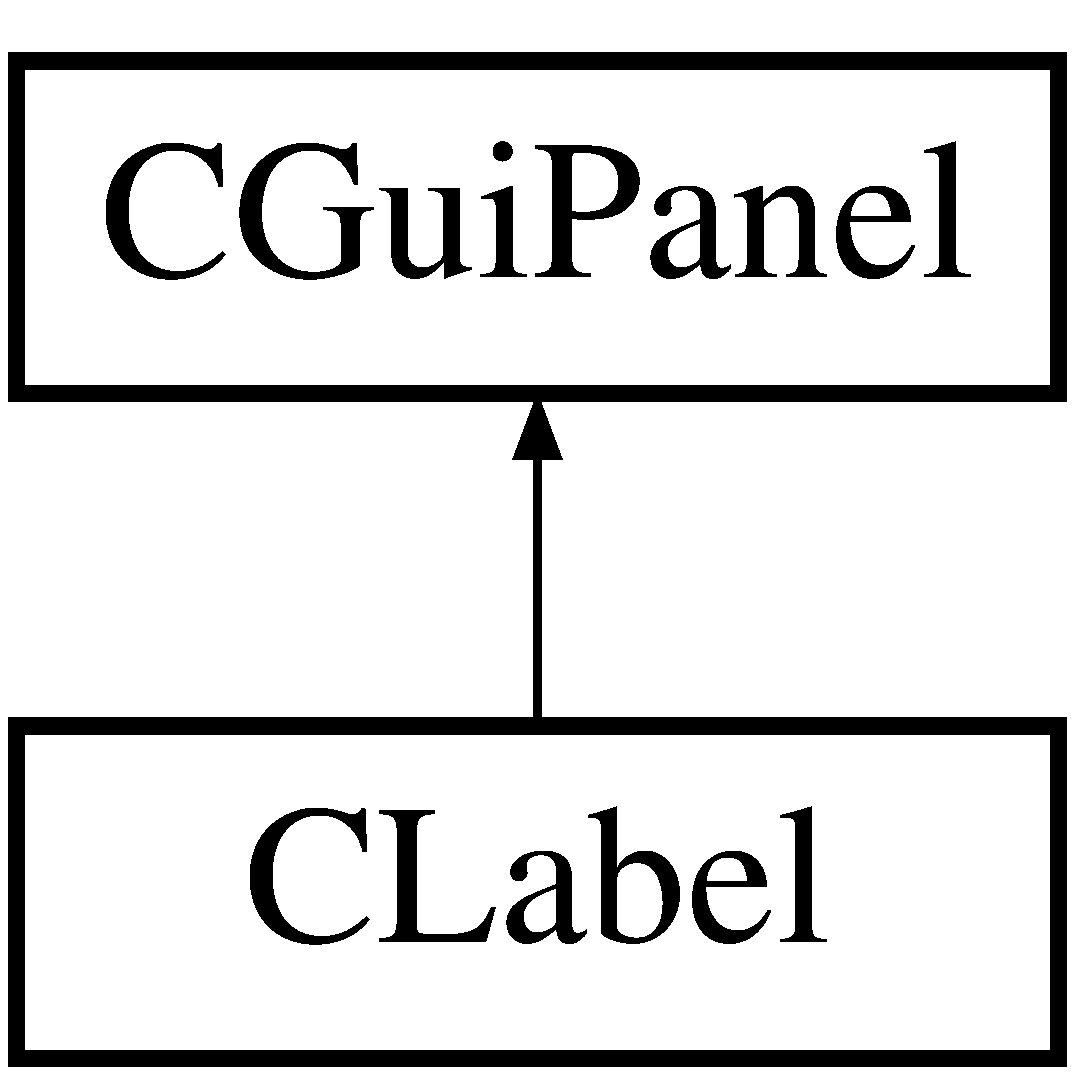
\includegraphics[height=2.000000cm]{class_c_label}
\end{center}
\end{figure}
\subsection*{Public Member Functions}
\begin{DoxyCompactItemize}
\item 
\hypertarget{class_c_label_a7a9403391654ab37d5b08d83f22f7297}{
{\bfseries CLabel} (const \hyperlink{classvec2d}{vec2d} \&position, const \hyperlink{classvec2d}{vec2d} \&size, const std::wstring \&text=L\char`\"{}\char`\"{})}
\label{class_c_label_a7a9403391654ab37d5b08d83f22f7297}

\item 
\hypertarget{class_c_label_a0e0203561ca39ce5818f9fbf358b94e2}{
void {\bfseries setText} (const std::wstring \&text)}
\label{class_c_label_a0e0203561ca39ce5818f9fbf358b94e2}

\item 
\hypertarget{class_c_label_abb48935a5dfa15a83f686f7932a0e876}{
std::wstring {\bfseries getText} ()}
\label{class_c_label_abb48935a5dfa15a83f686f7932a0e876}

\item 
\hypertarget{class_c_label_aa0694ff29b8d4cc14bc45d00863bb48c}{
virtual void {\bfseries draw} ()}
\label{class_c_label_aa0694ff29b8d4cc14bc45d00863bb48c}

\item 
\hypertarget{class_c_label_a6db8b77b75a008fce6970e1b80cc29e1}{
virtual void {\bfseries updateFont} ()}
\label{class_c_label_a6db8b77b75a008fce6970e1b80cc29e1}

\end{DoxyCompactItemize}
\subsection*{Protected Member Functions}
\begin{DoxyCompactItemize}
\item 
\hypertarget{class_c_label_ac80139bb1042d7778ff2b91c9500d557}{
void {\bfseries init} ()}
\label{class_c_label_ac80139bb1042d7778ff2b91c9500d557}

\end{DoxyCompactItemize}
\subsection*{Protected Attributes}
\begin{DoxyCompactItemize}
\item 
\hypertarget{class_c_label_ae593eee3349e51a5565c00a7643b4cee}{
std::wstring {\bfseries \_\-text}}
\label{class_c_label_ae593eee3349e51a5565c00a7643b4cee}

\item 
\hypertarget{class_c_label_a1d6dfac41eaad67fa576af9405deab6d}{
float {\bfseries \_\-height}}
\label{class_c_label_a1d6dfac41eaad67fa576af9405deab6d}

\item 
\hypertarget{class_c_label_a010aab1e4ba2d4bc487a59eb83af4507}{
\hyperlink{class_font}{Font} $\ast$ {\bfseries \_\-font}}
\label{class_c_label_a010aab1e4ba2d4bc487a59eb83af4507}

\end{DoxyCompactItemize}


The documentation for this class was generated from the following files:\begin{DoxyCompactItemize}
\item 
src/gui/CLabel.h\item 
src/gui/CLabel.cpp\end{DoxyCompactItemize}

\hypertarget{class_c_main_menu}{
\section{CMainMenu Class Reference}
\label{class_c_main_menu}\index{CMainMenu@{CMainMenu}}
}
Inheritance diagram for CMainMenu:\begin{figure}[H]
\begin{center}
\leavevmode
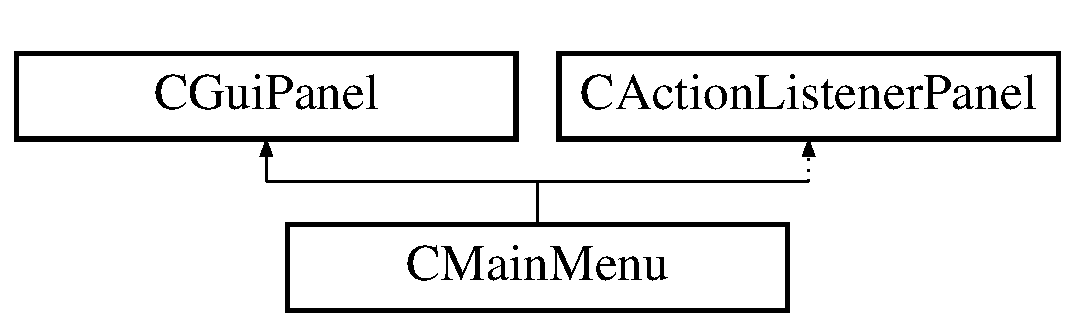
\includegraphics[height=2.000000cm]{class_c_main_menu}
\end{center}
\end{figure}
\subsection*{Public Member Functions}
\begin{DoxyCompactItemize}
\item 
\hypertarget{class_c_main_menu_a8591835e8b7d3514977b26eb442c81c8}{
virtual void {\bfseries draw} ()}
\label{class_c_main_menu_a8591835e8b7d3514977b26eb442c81c8}

\item 
\hypertarget{class_c_main_menu_ad5c15cb06e72a4d29eb9fb6f6e661e39}{
virtual void {\bfseries actionPerformed} (int id)}
\label{class_c_main_menu_ad5c15cb06e72a4d29eb9fb6f6e661e39}

\end{DoxyCompactItemize}
\subsection*{Protected Attributes}
\begin{DoxyCompactItemize}
\item 
\hypertarget{class_c_main_menu_a5e21dd2a3bcefaabe9c28701c8ccb224}{
\hyperlink{class_c_gui_panel}{CGuiPanel} $\ast$ {\bfseries newGame}}
\label{class_c_main_menu_a5e21dd2a3bcefaabe9c28701c8ccb224}

\item 
\hypertarget{class_c_main_menu_ad37150ce5163b9e3981924494726dae6}{
\hyperlink{class_c_gui_panel}{CGuiPanel} $\ast$ {\bfseries settings}}
\label{class_c_main_menu_ad37150ce5163b9e3981924494726dae6}

\item 
\hypertarget{class_c_main_menu_a3a06b14fa57be2ac155e6f2ceddecf90}{
double {\bfseries panelWidth}}
\label{class_c_main_menu_a3a06b14fa57be2ac155e6f2ceddecf90}

\end{DoxyCompactItemize}


The documentation for this class was generated from the following files:\begin{DoxyCompactItemize}
\item 
src/gui/CMainMenu.h\item 
src/gui/CMainMenu.cpp\end{DoxyCompactItemize}

\hypertarget{class_code_failure}{
\section{CodeFailure Class Reference}
\label{class_code_failure}\index{CodeFailure@{CodeFailure}}
}
\subsection*{Public Member Functions}
\begin{DoxyCompactItemize}
\item 
\hypertarget{class_code_failure_af67b88bfae4506c46155c9844dfd9d59}{
{\bfseries CodeFailure} (std::string line)}
\label{class_code_failure_af67b88bfae4506c46155c9844dfd9d59}

\end{DoxyCompactItemize}


The documentation for this class was generated from the following files:\begin{DoxyCompactItemize}
\item 
src/exceptions.h\item 
src/exceptions.cpp\end{DoxyCompactItemize}

\hypertarget{class_c_param_mgr}{
\section{CParamMgr Class Reference}
\label{class_c_param_mgr}\index{CParamMgr@{CParamMgr}}
}
\subsection*{Public Member Functions}
\begin{DoxyCompactItemize}
\item 
\hypertarget{class_c_param_mgr_a9782c5702391637f863ec6b5f3ded8cd}{
void {\bfseries linkVariableToParam} (void $\ast$memPointer, const std::string name)}
\label{class_c_param_mgr_a9782c5702391637f863ec6b5f3ded8cd}

\item 
\hypertarget{class_c_param_mgr_a54f329c9984f9bd815727e31a0ac09a9}{
void {\bfseries linkVariableToParam} (void $\ast$memPointer, const char $\ast$name)}
\label{class_c_param_mgr_a54f329c9984f9bd815727e31a0ac09a9}

\item 
\hypertarget{class_c_param_mgr_aad11c811d7df59fee55348863c5eb83f}{
std::string {\bfseries getStringParam} (std::string name)}
\label{class_c_param_mgr_aad11c811d7df59fee55348863c5eb83f}

\item 
\hypertarget{class_c_param_mgr_a2ffd91cd1e15d12386f61857611f0073}{
double {\bfseries getDoubleParam} (std::string name)}
\label{class_c_param_mgr_a2ffd91cd1e15d12386f61857611f0073}

\item 
\hypertarget{class_c_param_mgr_a3fa3412a604ac072f4055a5d3a560975}{
int {\bfseries getIntParam} (std::string name)}
\label{class_c_param_mgr_a3fa3412a604ac072f4055a5d3a560975}

\item 
\hypertarget{class_c_param_mgr_aa92e47cccb3007844d60b51b904c7f36}{
std::string {\bfseries setStringParam} (std::string name, std::string value)}
\label{class_c_param_mgr_aa92e47cccb3007844d60b51b904c7f36}

\item 
\hypertarget{class_c_param_mgr_abc525dbc23dcbc7471165f682fd8d434}{
double {\bfseries setDoubleParam} (std::string name, double value)}
\label{class_c_param_mgr_abc525dbc23dcbc7471165f682fd8d434}

\item 
\hypertarget{class_c_param_mgr_a66b81d0f97c7a413086361409c456926}{
int {\bfseries setIntParam} (std::string name, int value)}
\label{class_c_param_mgr_a66b81d0f97c7a413086361409c456926}

\end{DoxyCompactItemize}


The documentation for this class was generated from the following files:\begin{DoxyCompactItemize}
\item 
src/CParamMgr.h\item 
src/CParamMgr.cpp\end{DoxyCompactItemize}

\hypertarget{class_c_text_field}{
\section{CTextField Class Reference}
\label{class_c_text_field}\index{CTextField@{CTextField}}
}
Inheritance diagram for CTextField:\begin{figure}[H]
\begin{center}
\leavevmode
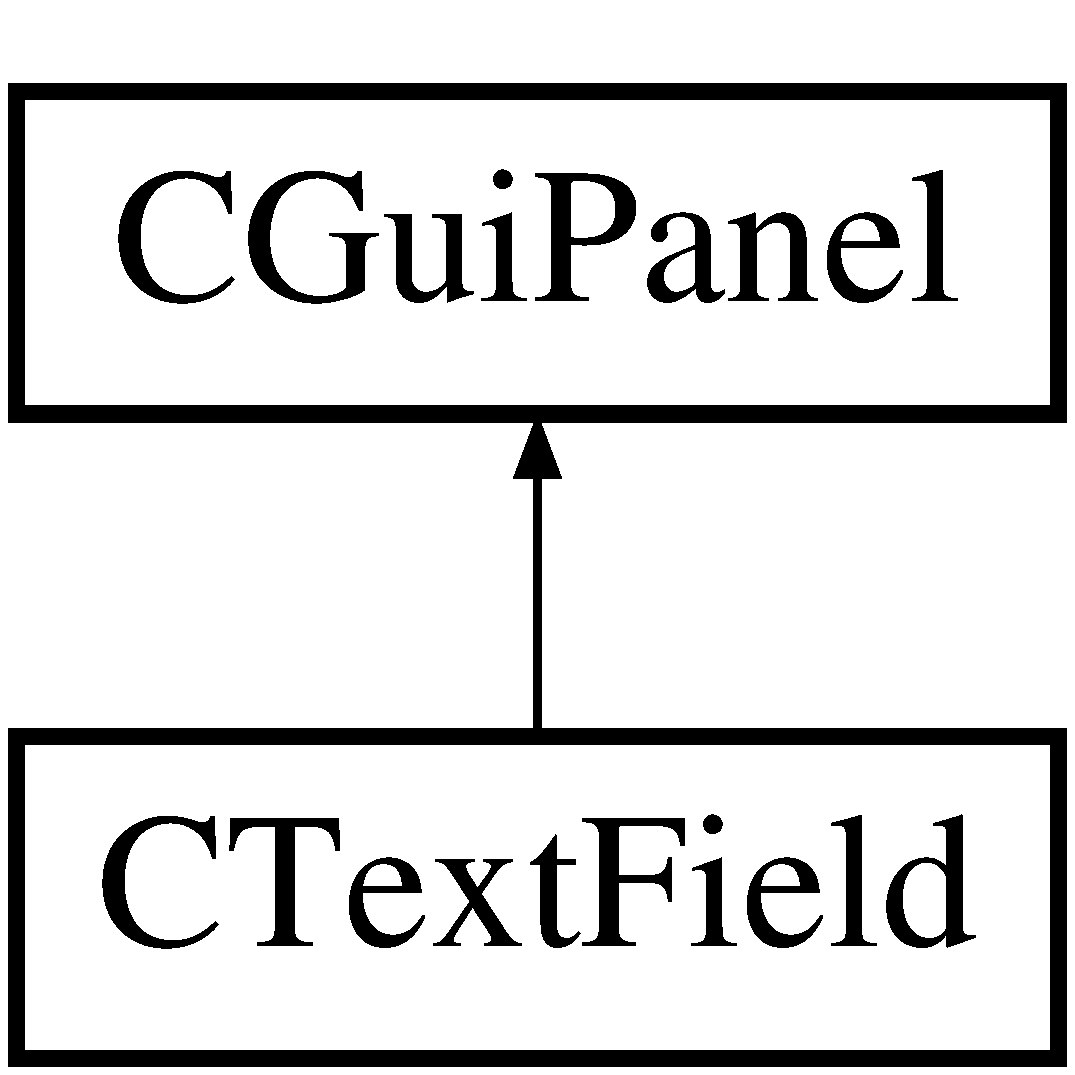
\includegraphics[height=2.000000cm]{class_c_text_field}
\end{center}
\end{figure}
\subsection*{Public Member Functions}
\begin{DoxyCompactItemize}
\item 
\hypertarget{class_c_text_field_a8a1d91c6f80ba3a98cfde80681705d74}{
{\bfseries CTextField} (const \hyperlink{classvec2d}{vec2d} \&position, const \hyperlink{classvec2d}{vec2d} \&size, const std::wstring \&text=L\char`\"{}\char`\"{})}
\label{class_c_text_field_a8a1d91c6f80ba3a98cfde80681705d74}

\item 
\hypertarget{class_c_text_field_aad1383591067e3ec981356e98e690dee}{
virtual void {\bfseries onKeyboard} (const std::wstring \&string)}
\label{class_c_text_field_aad1383591067e3ec981356e98e690dee}

\item 
\hypertarget{class_c_text_field_a7809dd12c6f601f6f52a39e1b8f36ff5}{
virtual void {\bfseries draw} ()}
\label{class_c_text_field_a7809dd12c6f601f6f52a39e1b8f36ff5}

\end{DoxyCompactItemize}
\subsection*{Protected Attributes}
\begin{DoxyCompactItemize}
\item 
\hypertarget{class_c_text_field_a26bd78e5a1a4609dbaae13f40cd1a5e1}{
std::wstring {\bfseries \_\-string}}
\label{class_c_text_field_a26bd78e5a1a4609dbaae13f40cd1a5e1}

\item 
\hypertarget{class_c_text_field_a8f399613b03fbf9017ba7dd49f22244e}{
\hyperlink{class_c_label}{CLabel} $\ast$ {\bfseries \_\-label}}
\label{class_c_text_field_a8f399613b03fbf9017ba7dd49f22244e}

\end{DoxyCompactItemize}


The documentation for this class was generated from the following files:\begin{DoxyCompactItemize}
\item 
src/gui/CTextField.h\item 
src/gui/CTextField.cpp\end{DoxyCompactItemize}

\hypertarget{class_c_window}{
\section{CWindow Class Reference}
\label{class_c_window}\index{CWindow@{CWindow}}
}
Inheritance diagram for CWindow:\begin{figure}[H]
\begin{center}
\leavevmode
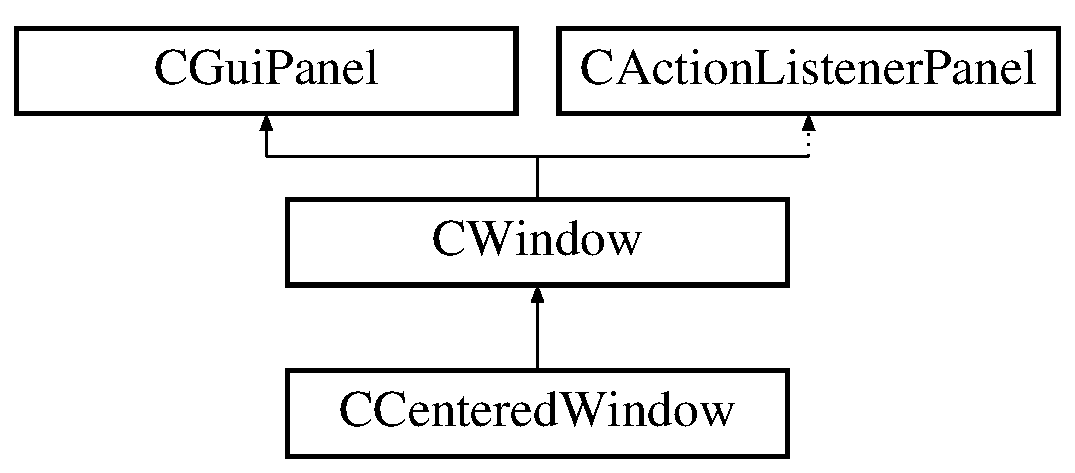
\includegraphics[height=3.000000cm]{class_c_window}
\end{center}
\end{figure}
\subsection*{Public Member Functions}
\begin{DoxyCompactItemize}
\item 
\hypertarget{class_c_window_affbb54629e50a18e9e8c8a35987c3856}{
{\bfseries CWindow} (const \hyperlink{classvec2d}{vec2d} \&position, const \hyperlink{classvec2d}{vec2d} \&size, const std::wstring \&label)}
\label{class_c_window_affbb54629e50a18e9e8c8a35987c3856}

\item 
\hypertarget{class_c_window_a433a3a123bc902f57a204c3970f3fd51}{
virtual void {\bfseries draw} ()}
\label{class_c_window_a433a3a123bc902f57a204c3970f3fd51}

\item 
\hypertarget{class_c_window_adbf4dacd60a4ffea05fed1bab58c8266}{
virtual void {\bfseries actionPerformed} (int id)}
\label{class_c_window_adbf4dacd60a4ffea05fed1bab58c8266}

\item 
\hypertarget{class_c_window_a4143fd3618ac04f39242a649d1e9a1a5}{
virtual void {\bfseries onMouseDown} (const \hyperlink{classvec2d}{vec2d} \&position, const MouseButton button)}
\label{class_c_window_a4143fd3618ac04f39242a649d1e9a1a5}

\end{DoxyCompactItemize}


The documentation for this class was generated from the following files:\begin{DoxyCompactItemize}
\item 
src/gui/CWindow.h\item 
src/gui/CWindow.cpp\end{DoxyCompactItemize}

\hypertarget{structent_param}{
\section{entParam Struct Reference}
\label{structent_param}\index{entParam@{entParam}}
}
\subsection*{Public Attributes}
\begin{DoxyCompactItemize}
\item 
\hypertarget{structent_param_a65f11d247a04ad2cca85a2ba0ef6e5df}{
void $\ast$ {\bfseries memPointer}}
\label{structent_param_a65f11d247a04ad2cca85a2ba0ef6e5df}

\item 
\hypertarget{structent_param_aaec0219278075d5cae2e458ffecbe75b}{
std::string {\bfseries name}}
\label{structent_param_aaec0219278075d5cae2e458ffecbe75b}

\item 
\hypertarget{structent_param_a85f8333383325bf46fa7f20d44d86bfe}{
DATATYPE {\bfseries type}}
\label{structent_param_a85f8333383325bf46fa7f20d44d86bfe}

\end{DoxyCompactItemize}


The documentation for this struct was generated from the following file:\begin{DoxyCompactItemize}
\item 
src/datatypes.h\end{DoxyCompactItemize}

\hypertarget{class_font}{
\section{Font Class Reference}
\label{class_font}\index{Font@{Font}}
}
\subsection*{Public Member Functions}
\begin{DoxyCompactItemize}
\item 
\hypertarget{class_font_a655b8b32288541d5f6e988f35f3cc842}{
void {\bfseries render} (const \hyperlink{classvec2d}{vec2d} \&pos, const double size, const std::wstring \&text, const \hyperlink{classrgba}{rgba} \&color)}
\label{class_font_a655b8b32288541d5f6e988f35f3cc842}

\item 
\hypertarget{class_font_ae8143429d803e39132940a490c1621c7}{
void {\bfseries render} (const \hyperlink{classvec2d}{vec2d} \&pos, const double size, const std::wstring \&text)}
\label{class_font_ae8143429d803e39132940a490c1621c7}

\item 
\hypertarget{class_font_af1d03f62c12e4bf1982739ea7816dfa6}{
void {\bfseries render} (const double size, const std::wstring \&text)}
\label{class_font_af1d03f62c12e4bf1982739ea7816dfa6}

\item 
\hypertarget{class_font_ac4b7f5628cf8f33d03fc3183e0c69e64}{
void {\bfseries render} (const double size, const std::wstring \&text, const \hyperlink{classrgba}{rgba} \&color)}
\label{class_font_ac4b7f5628cf8f33d03fc3183e0c69e64}

\item 
\hypertarget{class_font_acc434587d0bc0a17bf04a65ad1214a9c}{
void {\bfseries setSize} (const int size)}
\label{class_font_acc434587d0bc0a17bf04a65ad1214a9c}

\end{DoxyCompactItemize}
\subsection*{Friends}
\begin{DoxyCompactItemize}
\item 
\hypertarget{class_font_a6ad503389779bbc2d3efa7456d87ed3c}{
class \hyperlink{class_font_a6ad503389779bbc2d3efa7456d87ed3c}{CFontMgr}}
\label{class_font_a6ad503389779bbc2d3efa7456d87ed3c}

\end{DoxyCompactItemize}


The documentation for this class was generated from the following files:\begin{DoxyCompactItemize}
\item 
src/Font.h\item 
src/Font.cpp\end{DoxyCompactItemize}

\hypertarget{struct_f_t___auto_hinter___service_rec__}{
\section{FT\_\-AutoHinter\_\-ServiceRec\_\- Struct Reference}
\label{struct_f_t___auto_hinter___service_rec__}\index{FT\_\-AutoHinter\_\-ServiceRec\_\-@{FT\_\-AutoHinter\_\-ServiceRec\_\-}}
}
\subsection*{Public Attributes}
\begin{DoxyCompactItemize}
\item 
\hypertarget{struct_f_t___auto_hinter___service_rec___a846234a9c9c5427d3274e4568f33272c}{
FT\_\-AutoHinter\_\-GlobalResetFunc {\bfseries reset\_\-face}}
\label{struct_f_t___auto_hinter___service_rec___a846234a9c9c5427d3274e4568f33272c}

\item 
\hypertarget{struct_f_t___auto_hinter___service_rec___a958371c33e08125393cd4b401a22f2a0}{
FT\_\-AutoHinter\_\-GlobalGetFunc {\bfseries get\_\-global\_\-hints}}
\label{struct_f_t___auto_hinter___service_rec___a958371c33e08125393cd4b401a22f2a0}

\item 
\hypertarget{struct_f_t___auto_hinter___service_rec___a648ac943fc1194f60ba638e0a59486e9}{
FT\_\-AutoHinter\_\-GlobalDoneFunc {\bfseries done\_\-global\_\-hints}}
\label{struct_f_t___auto_hinter___service_rec___a648ac943fc1194f60ba638e0a59486e9}

\item 
\hypertarget{struct_f_t___auto_hinter___service_rec___ad36efe39469959626744ebdd04a04031}{
FT\_\-AutoHinter\_\-GlyphLoadFunc {\bfseries load\_\-glyph}}
\label{struct_f_t___auto_hinter___service_rec___ad36efe39469959626744ebdd04a04031}

\end{DoxyCompactItemize}


The documentation for this struct was generated from the following file:\begin{DoxyCompactItemize}
\item 
src/libs/freetype/internal/autohint.h\end{DoxyCompactItemize}

\hypertarget{struct_f_t___b_box__}{
\section{FT\_\-BBox\_\- Struct Reference}
\label{struct_f_t___b_box__}\index{FT\_\-BBox\_\-@{FT\_\-BBox\_\-}}
}
\subsection*{Public Attributes}
\begin{DoxyCompactItemize}
\item 
\hypertarget{struct_f_t___b_box___a1f2a5d0565d496c1d41e43d018f45add}{
FT\_\-Pos {\bfseries xMin}}
\label{struct_f_t___b_box___a1f2a5d0565d496c1d41e43d018f45add}

\item 
\hypertarget{struct_f_t___b_box___a959ca1d5bc1c5338da0d85c8e7135f4e}{
FT\_\-Pos {\bfseries yMin}}
\label{struct_f_t___b_box___a959ca1d5bc1c5338da0d85c8e7135f4e}

\item 
\hypertarget{struct_f_t___b_box___ac6da5c44f4cb7b97eef1f438eb69c0ec}{
FT\_\-Pos {\bfseries xMax}}
\label{struct_f_t___b_box___ac6da5c44f4cb7b97eef1f438eb69c0ec}

\item 
\hypertarget{struct_f_t___b_box___a77084921589f386a8a593ae1f25b1569}{
FT\_\-Pos {\bfseries yMax}}
\label{struct_f_t___b_box___a77084921589f386a8a593ae1f25b1569}

\end{DoxyCompactItemize}


The documentation for this struct was generated from the following file:\begin{DoxyCompactItemize}
\item 
src/libs/freetype/ftimage.h\end{DoxyCompactItemize}

\hypertarget{struct_f_t___bitmap__}{
\section{FT\_\-Bitmap\_\- Struct Reference}
\label{struct_f_t___bitmap__}\index{FT\_\-Bitmap\_\-@{FT\_\-Bitmap\_\-}}
}
\subsection*{Public Attributes}
\begin{DoxyCompactItemize}
\item 
\hypertarget{struct_f_t___bitmap___a1b6bb20b30fe087e3fc87a0eb37730c0}{
int {\bfseries rows}}
\label{struct_f_t___bitmap___a1b6bb20b30fe087e3fc87a0eb37730c0}

\item 
\hypertarget{struct_f_t___bitmap___a7b5e6252dd91a3809fe80ebbeb6720eb}{
int {\bfseries width}}
\label{struct_f_t___bitmap___a7b5e6252dd91a3809fe80ebbeb6720eb}

\item 
\hypertarget{struct_f_t___bitmap___afdee595846e1188c7a76d0cec9d85cf2}{
int {\bfseries pitch}}
\label{struct_f_t___bitmap___afdee595846e1188c7a76d0cec9d85cf2}

\item 
\hypertarget{struct_f_t___bitmap___a76439b1d3c13b81ca506108cd1623284}{
unsigned char $\ast$ {\bfseries buffer}}
\label{struct_f_t___bitmap___a76439b1d3c13b81ca506108cd1623284}

\item 
\hypertarget{struct_f_t___bitmap___a415d78060f8012d312703c9792ec005a}{
short {\bfseries num\_\-grays}}
\label{struct_f_t___bitmap___a415d78060f8012d312703c9792ec005a}

\item 
\hypertarget{struct_f_t___bitmap___a5cc5e0fe42a93a86e16706ad52e087a2}{
char {\bfseries pixel\_\-mode}}
\label{struct_f_t___bitmap___a5cc5e0fe42a93a86e16706ad52e087a2}

\item 
\hypertarget{struct_f_t___bitmap___ae7c8c74255cd27873b12a360cd5f3884}{
char {\bfseries palette\_\-mode}}
\label{struct_f_t___bitmap___ae7c8c74255cd27873b12a360cd5f3884}

\item 
\hypertarget{struct_f_t___bitmap___a8d5ecf4409f71bfb559e0d13d8df4d86}{
void $\ast$ {\bfseries palette}}
\label{struct_f_t___bitmap___a8d5ecf4409f71bfb559e0d13d8df4d86}

\end{DoxyCompactItemize}


The documentation for this struct was generated from the following file:\begin{DoxyCompactItemize}
\item 
src/libs/freetype/ftimage.h\end{DoxyCompactItemize}

\hypertarget{struct_f_t___bitmap___size__}{
\section{FT\_\-Bitmap\_\-Size\_\- Struct Reference}
\label{struct_f_t___bitmap___size__}\index{FT\_\-Bitmap\_\-Size\_\-@{FT\_\-Bitmap\_\-Size\_\-}}
}
\subsection*{Public Attributes}
\begin{DoxyCompactItemize}
\item 
\hypertarget{struct_f_t___bitmap___size___adf2f24039b458ff4674712886f242262}{
FT\_\-Short {\bfseries height}}
\label{struct_f_t___bitmap___size___adf2f24039b458ff4674712886f242262}

\item 
\hypertarget{struct_f_t___bitmap___size___ab9da94223f75a89a649d1e6d018b17f1}{
FT\_\-Short {\bfseries width}}
\label{struct_f_t___bitmap___size___ab9da94223f75a89a649d1e6d018b17f1}

\item 
\hypertarget{struct_f_t___bitmap___size___a1db23a6220fb6bcb712430821a6e5352}{
FT\_\-Pos {\bfseries size}}
\label{struct_f_t___bitmap___size___a1db23a6220fb6bcb712430821a6e5352}

\item 
\hypertarget{struct_f_t___bitmap___size___a6f877a792d2dc93328037c928979215f}{
FT\_\-Pos {\bfseries x\_\-ppem}}
\label{struct_f_t___bitmap___size___a6f877a792d2dc93328037c928979215f}

\item 
\hypertarget{struct_f_t___bitmap___size___a60d4d003d09fd57505f69f39e31e19c1}{
FT\_\-Pos {\bfseries y\_\-ppem}}
\label{struct_f_t___bitmap___size___a60d4d003d09fd57505f69f39e31e19c1}

\end{DoxyCompactItemize}


The documentation for this struct was generated from the following file:\begin{DoxyCompactItemize}
\item 
src/libs/freetype/freetype.h\end{DoxyCompactItemize}

\hypertarget{struct_f_t___bitmap_glyph_rec__}{
\section{FT\_\-BitmapGlyphRec\_\- Struct Reference}
\label{struct_f_t___bitmap_glyph_rec__}\index{FT\_\-BitmapGlyphRec\_\-@{FT\_\-BitmapGlyphRec\_\-}}
}
\subsection*{Public Attributes}
\begin{DoxyCompactItemize}
\item 
\hypertarget{struct_f_t___bitmap_glyph_rec___ac3970353fbc0fe3d4c59c3fd608140f3}{
\hyperlink{struct_f_t___glyph_rec__}{FT\_\-GlyphRec} {\bfseries root}}
\label{struct_f_t___bitmap_glyph_rec___ac3970353fbc0fe3d4c59c3fd608140f3}

\item 
\hypertarget{struct_f_t___bitmap_glyph_rec___a6cfd2d89af7b6be4af886047c9cb7e0a}{
FT\_\-Int {\bfseries left}}
\label{struct_f_t___bitmap_glyph_rec___a6cfd2d89af7b6be4af886047c9cb7e0a}

\item 
\hypertarget{struct_f_t___bitmap_glyph_rec___a25fc81296678d6a2d064843c01bc05f7}{
FT\_\-Int {\bfseries top}}
\label{struct_f_t___bitmap_glyph_rec___a25fc81296678d6a2d064843c01bc05f7}

\item 
\hypertarget{struct_f_t___bitmap_glyph_rec___a16ecd0725920f8d5ad4c14e9448126ad}{
\hyperlink{struct_f_t___bitmap__}{FT\_\-Bitmap} {\bfseries bitmap}}
\label{struct_f_t___bitmap_glyph_rec___a16ecd0725920f8d5ad4c14e9448126ad}

\end{DoxyCompactItemize}


The documentation for this struct was generated from the following file:\begin{DoxyCompactItemize}
\item 
src/libs/freetype/ftglyph.h\end{DoxyCompactItemize}

\hypertarget{struct_f_t___char_map_rec__}{
\section{FT\_\-CharMapRec\_\- Struct Reference}
\label{struct_f_t___char_map_rec__}\index{FT\_\-CharMapRec\_\-@{FT\_\-CharMapRec\_\-}}
}
\subsection*{Public Attributes}
\begin{DoxyCompactItemize}
\item 
\hypertarget{struct_f_t___char_map_rec___a70a4e53e3f9818209916e5745c46dc28}{
\hyperlink{struct_f_t___face_rec__}{FT\_\-Face} {\bfseries face}}
\label{struct_f_t___char_map_rec___a70a4e53e3f9818209916e5745c46dc28}

\item 
\hypertarget{struct_f_t___char_map_rec___a88ee6f726ef11a8e6cc793d59ff5557e}{
FT\_\-Encoding {\bfseries encoding}}
\label{struct_f_t___char_map_rec___a88ee6f726ef11a8e6cc793d59ff5557e}

\item 
\hypertarget{struct_f_t___char_map_rec___ae7f439996a8615698e780ce3c4f92457}{
FT\_\-UShort {\bfseries platform\_\-id}}
\label{struct_f_t___char_map_rec___ae7f439996a8615698e780ce3c4f92457}

\item 
\hypertarget{struct_f_t___char_map_rec___af10dd43eee8dc93e7d6191c663ae831a}{
FT\_\-UShort {\bfseries encoding\_\-id}}
\label{struct_f_t___char_map_rec___af10dd43eee8dc93e7d6191c663ae831a}

\end{DoxyCompactItemize}


The documentation for this struct was generated from the following file:\begin{DoxyCompactItemize}
\item 
src/libs/freetype/freetype.h\end{DoxyCompactItemize}

\hypertarget{struct_f_t___c_map___class_rec__}{
\section{FT\_\-CMap\_\-ClassRec\_\- Struct Reference}
\label{struct_f_t___c_map___class_rec__}\index{FT\_\-CMap\_\-ClassRec\_\-@{FT\_\-CMap\_\-ClassRec\_\-}}
}
\subsection*{Public Attributes}
\begin{DoxyCompactItemize}
\item 
\hypertarget{struct_f_t___c_map___class_rec___a86283cf239b9c0e559c9acbaa004def6}{
FT\_\-ULong {\bfseries size}}
\label{struct_f_t___c_map___class_rec___a86283cf239b9c0e559c9acbaa004def6}

\item 
\hypertarget{struct_f_t___c_map___class_rec___afe1da0877ec0686dfe7b2e020fc0d408}{
FT\_\-CMap\_\-InitFunc {\bfseries init}}
\label{struct_f_t___c_map___class_rec___afe1da0877ec0686dfe7b2e020fc0d408}

\item 
\hypertarget{struct_f_t___c_map___class_rec___a00d1d77a4d926340b4d97bc03cd29231}{
FT\_\-CMap\_\-DoneFunc {\bfseries done}}
\label{struct_f_t___c_map___class_rec___a00d1d77a4d926340b4d97bc03cd29231}

\item 
\hypertarget{struct_f_t___c_map___class_rec___ad1c0448188e8d52f6159b5521bb2dc83}{
FT\_\-CMap\_\-CharIndexFunc {\bfseries char\_\-index}}
\label{struct_f_t___c_map___class_rec___ad1c0448188e8d52f6159b5521bb2dc83}

\item 
\hypertarget{struct_f_t___c_map___class_rec___a053362f31fcfbc6a284cc8d026ab57ff}{
FT\_\-CMap\_\-CharNextFunc {\bfseries char\_\-next}}
\label{struct_f_t___c_map___class_rec___a053362f31fcfbc6a284cc8d026ab57ff}

\item 
\hypertarget{struct_f_t___c_map___class_rec___a6bc46e2595aec30295e6d2bfc362afcb}{
FT\_\-CMap\_\-CharVarIndexFunc {\bfseries char\_\-var\_\-index}}
\label{struct_f_t___c_map___class_rec___a6bc46e2595aec30295e6d2bfc362afcb}

\item 
\hypertarget{struct_f_t___c_map___class_rec___ac8305cb0aebd02b54c0046765f28ef4a}{
FT\_\-CMap\_\-CharVarIsDefaultFunc {\bfseries char\_\-var\_\-default}}
\label{struct_f_t___c_map___class_rec___ac8305cb0aebd02b54c0046765f28ef4a}

\item 
\hypertarget{struct_f_t___c_map___class_rec___ad61635444cbfc71c4259e74cb892c172}{
FT\_\-CMap\_\-VariantListFunc {\bfseries variant\_\-list}}
\label{struct_f_t___c_map___class_rec___ad61635444cbfc71c4259e74cb892c172}

\item 
\hypertarget{struct_f_t___c_map___class_rec___a65db9dfa0e29b7de257dc8870532ab19}{
FT\_\-CMap\_\-CharVariantListFunc {\bfseries charvariant\_\-list}}
\label{struct_f_t___c_map___class_rec___a65db9dfa0e29b7de257dc8870532ab19}

\item 
\hypertarget{struct_f_t___c_map___class_rec___ac1563590a0bac99082aa0996b94aad57}{
FT\_\-CMap\_\-VariantCharListFunc {\bfseries variantchar\_\-list}}
\label{struct_f_t___c_map___class_rec___ac1563590a0bac99082aa0996b94aad57}

\end{DoxyCompactItemize}


The documentation for this struct was generated from the following file:\begin{DoxyCompactItemize}
\item 
src/libs/freetype/internal/ftobjs.h\end{DoxyCompactItemize}

\hypertarget{struct_f_t___c_map_rec__}{
\section{FT\_\-CMapRec\_\- Struct Reference}
\label{struct_f_t___c_map_rec__}\index{FT\_\-CMapRec\_\-@{FT\_\-CMapRec\_\-}}
}
\subsection*{Public Attributes}
\begin{DoxyCompactItemize}
\item 
\hypertarget{struct_f_t___c_map_rec___a39fa6de9995d4ae4496b93e2b874b34e}{
\hyperlink{struct_f_t___char_map_rec__}{FT\_\-CharMapRec} {\bfseries charmap}}
\label{struct_f_t___c_map_rec___a39fa6de9995d4ae4496b93e2b874b34e}

\item 
\hypertarget{struct_f_t___c_map_rec___aa85db42650df0edb38f8af5887c0ac6a}{
\hyperlink{struct_f_t___c_map___class_rec__}{FT\_\-CMap\_\-Class} {\bfseries clazz}}
\label{struct_f_t___c_map_rec___aa85db42650df0edb38f8af5887c0ac6a}

\end{DoxyCompactItemize}


The documentation for this struct was generated from the following file:\begin{DoxyCompactItemize}
\item 
src/libs/freetype/internal/ftobjs.h\end{DoxyCompactItemize}

\hypertarget{struct_f_t___data__}{
\section{FT\_\-Data\_\- Struct Reference}
\label{struct_f_t___data__}\index{FT\_\-Data\_\-@{FT\_\-Data\_\-}}
}
\subsection*{Public Attributes}
\begin{DoxyCompactItemize}
\item 
\hypertarget{struct_f_t___data___a4dea731b8a256b973757e1b8f612b050}{
const FT\_\-Byte $\ast$ {\bfseries pointer}}
\label{struct_f_t___data___a4dea731b8a256b973757e1b8f612b050}

\item 
\hypertarget{struct_f_t___data___af60c89dccd1852aceb0dc08675aca2fd}{
FT\_\-Int {\bfseries length}}
\label{struct_f_t___data___af60c89dccd1852aceb0dc08675aca2fd}

\end{DoxyCompactItemize}


The documentation for this struct was generated from the following file:\begin{DoxyCompactItemize}
\item 
src/libs/freetype/fttypes.h\end{DoxyCompactItemize}

\hypertarget{struct_f_t___driver___class_rec__}{
\section{FT\_\-Driver\_\-ClassRec\_\- Struct Reference}
\label{struct_f_t___driver___class_rec__}\index{FT\_\-Driver\_\-ClassRec\_\-@{FT\_\-Driver\_\-ClassRec\_\-}}
}
\subsection*{Public Attributes}
\begin{DoxyCompactItemize}
\item 
\hypertarget{struct_f_t___driver___class_rec___a087ca3e2c562bb90b8af82b31e82d8c7}{
\hyperlink{struct_f_t___module___class__}{FT\_\-Module\_\-Class} {\bfseries root}}
\label{struct_f_t___driver___class_rec___a087ca3e2c562bb90b8af82b31e82d8c7}

\item 
\hypertarget{struct_f_t___driver___class_rec___a194fc6fbae019e9c109c65328e57e44f}{
FT\_\-Long {\bfseries face\_\-object\_\-size}}
\label{struct_f_t___driver___class_rec___a194fc6fbae019e9c109c65328e57e44f}

\item 
\hypertarget{struct_f_t___driver___class_rec___a436687825ee47ed94da71fda90e2f578}{
FT\_\-Long {\bfseries size\_\-object\_\-size}}
\label{struct_f_t___driver___class_rec___a436687825ee47ed94da71fda90e2f578}

\item 
\hypertarget{struct_f_t___driver___class_rec___adcce7eb86dd7c763b622818cfcde99a6}{
FT\_\-Long {\bfseries slot\_\-object\_\-size}}
\label{struct_f_t___driver___class_rec___adcce7eb86dd7c763b622818cfcde99a6}

\item 
\hypertarget{struct_f_t___driver___class_rec___a68e94aeae3e78ed5984c29189c64df9a}{
FT\_\-Face\_\-InitFunc {\bfseries init\_\-face}}
\label{struct_f_t___driver___class_rec___a68e94aeae3e78ed5984c29189c64df9a}

\item 
\hypertarget{struct_f_t___driver___class_rec___a7d37afe63f914ae28ed02c960e4d5642}{
FT\_\-Face\_\-DoneFunc {\bfseries done\_\-face}}
\label{struct_f_t___driver___class_rec___a7d37afe63f914ae28ed02c960e4d5642}

\item 
\hypertarget{struct_f_t___driver___class_rec___a0aec58307bc166f0e74c890509638ddf}{
FT\_\-Size\_\-InitFunc {\bfseries init\_\-size}}
\label{struct_f_t___driver___class_rec___a0aec58307bc166f0e74c890509638ddf}

\item 
\hypertarget{struct_f_t___driver___class_rec___a5c96f627816a089b27bcff09f22dd1a6}{
FT\_\-Size\_\-DoneFunc {\bfseries done\_\-size}}
\label{struct_f_t___driver___class_rec___a5c96f627816a089b27bcff09f22dd1a6}

\item 
\hypertarget{struct_f_t___driver___class_rec___ae4e1d4ec7bdbdee0b4a5f8fc8f113d30}{
FT\_\-Slot\_\-InitFunc {\bfseries init\_\-slot}}
\label{struct_f_t___driver___class_rec___ae4e1d4ec7bdbdee0b4a5f8fc8f113d30}

\item 
\hypertarget{struct_f_t___driver___class_rec___a548a343f5921f5d341142bf3743c42d4}{
FT\_\-Slot\_\-DoneFunc {\bfseries done\_\-slot}}
\label{struct_f_t___driver___class_rec___a548a343f5921f5d341142bf3743c42d4}

\item 
\hypertarget{struct_f_t___driver___class_rec___a49dbd71e64094d4d825b8b8d51dd4e47}{
FT\_\-Slot\_\-LoadFunc {\bfseries load\_\-glyph}}
\label{struct_f_t___driver___class_rec___a49dbd71e64094d4d825b8b8d51dd4e47}

\item 
\hypertarget{struct_f_t___driver___class_rec___a398395bfdbef65a8d531724d200ed91c}{
FT\_\-Face\_\-GetKerningFunc {\bfseries get\_\-kerning}}
\label{struct_f_t___driver___class_rec___a398395bfdbef65a8d531724d200ed91c}

\item 
\hypertarget{struct_f_t___driver___class_rec___a9caec9ae56a4bab9c90cede699279f29}{
FT\_\-Face\_\-AttachFunc {\bfseries attach\_\-file}}
\label{struct_f_t___driver___class_rec___a9caec9ae56a4bab9c90cede699279f29}

\item 
\hypertarget{struct_f_t___driver___class_rec___aad560cd145b6d7cab7eae79194b1d724}{
FT\_\-Face\_\-GetAdvancesFunc {\bfseries get\_\-advances}}
\label{struct_f_t___driver___class_rec___aad560cd145b6d7cab7eae79194b1d724}

\item 
\hypertarget{struct_f_t___driver___class_rec___a03ff7c2e4a2fb6d08eb481b03a78e8de}{
FT\_\-Size\_\-RequestFunc {\bfseries request\_\-size}}
\label{struct_f_t___driver___class_rec___a03ff7c2e4a2fb6d08eb481b03a78e8de}

\item 
\hypertarget{struct_f_t___driver___class_rec___a1b365eb82525dae0a816974d949fe0dd}{
FT\_\-Size\_\-SelectFunc {\bfseries select\_\-size}}
\label{struct_f_t___driver___class_rec___a1b365eb82525dae0a816974d949fe0dd}

\end{DoxyCompactItemize}


The documentation for this struct was generated from the following file:\begin{DoxyCompactItemize}
\item 
src/libs/freetype/internal/ftdriver.h\end{DoxyCompactItemize}

\hypertarget{struct_f_t___driver_rec__}{
\section{FT\_\-DriverRec\_\- Struct Reference}
\label{struct_f_t___driver_rec__}\index{FT\_\-DriverRec\_\-@{FT\_\-DriverRec\_\-}}
}
\subsection*{Public Attributes}
\begin{DoxyCompactItemize}
\item 
\hypertarget{struct_f_t___driver_rec___a8451ceb25c76794fb47e81f477c8222d}{
\hyperlink{struct_f_t___module_rec__}{FT\_\-ModuleRec} {\bfseries root}}
\label{struct_f_t___driver_rec___a8451ceb25c76794fb47e81f477c8222d}

\item 
\hypertarget{struct_f_t___driver_rec___a3111153608e5abeb093ed5eb7fef5aec}{
\hyperlink{struct_f_t___driver___class_rec__}{FT\_\-Driver\_\-Class} {\bfseries clazz}}
\label{struct_f_t___driver_rec___a3111153608e5abeb093ed5eb7fef5aec}

\item 
\hypertarget{struct_f_t___driver_rec___a2602170e3ecde21a764dc32417aaa002}{
\hyperlink{struct_f_t___list_rec__}{FT\_\-ListRec} {\bfseries faces\_\-list}}
\label{struct_f_t___driver_rec___a2602170e3ecde21a764dc32417aaa002}

\item 
\hypertarget{struct_f_t___driver_rec___ad2f1c1a800723dc887dcbc7ce78203d8}{
void $\ast$ {\bfseries extensions}}
\label{struct_f_t___driver_rec___ad2f1c1a800723dc887dcbc7ce78203d8}

\item 
\hypertarget{struct_f_t___driver_rec___ac28e7adbc14ee82c2b7710d0ee5541e2}{
FT\_\-GlyphLoader {\bfseries glyph\_\-loader}}
\label{struct_f_t___driver_rec___ac28e7adbc14ee82c2b7710d0ee5541e2}

\end{DoxyCompactItemize}


The documentation for this struct was generated from the following file:\begin{DoxyCompactItemize}
\item 
src/libs/freetype/internal/ftobjs.h\end{DoxyCompactItemize}

\hypertarget{struct_f_t___face___internal_rec__}{
\section{FT\_\-Face\_\-InternalRec\_\- Struct Reference}
\label{struct_f_t___face___internal_rec__}\index{FT\_\-Face\_\-InternalRec\_\-@{FT\_\-Face\_\-InternalRec\_\-}}
}
\subsection*{Public Attributes}
\begin{DoxyCompactItemize}
\item 
\hypertarget{struct_f_t___face___internal_rec___ab4be2dcda098e6136f5701580d18032d}{
\hyperlink{struct_f_t___matrix__}{FT\_\-Matrix} {\bfseries transform\_\-matrix}}
\label{struct_f_t___face___internal_rec___ab4be2dcda098e6136f5701580d18032d}

\item 
\hypertarget{struct_f_t___face___internal_rec___ab6c2aacdac58312273395b21b8d168c6}{
\hyperlink{struct_f_t___vector__}{FT\_\-Vector} {\bfseries transform\_\-delta}}
\label{struct_f_t___face___internal_rec___ab6c2aacdac58312273395b21b8d168c6}

\item 
\hypertarget{struct_f_t___face___internal_rec___a2495aced35040e1b7c2bc0afcd7a920d}{
FT\_\-Int {\bfseries transform\_\-flags}}
\label{struct_f_t___face___internal_rec___a2495aced35040e1b7c2bc0afcd7a920d}

\item 
\hypertarget{struct_f_t___face___internal_rec___abc3acb3bf5db056bb9c549af04f07963}{
\hyperlink{struct_f_t___service_cache_rec__}{FT\_\-ServiceCacheRec} {\bfseries services}}
\label{struct_f_t___face___internal_rec___abc3acb3bf5db056bb9c549af04f07963}

\item 
\hypertarget{struct_f_t___face___internal_rec___af898fd754c36c3f34c9ce0e88eb101c9}{
FT\_\-Bool {\bfseries ignore\_\-unpatented\_\-hinter}}
\label{struct_f_t___face___internal_rec___af898fd754c36c3f34c9ce0e88eb101c9}

\end{DoxyCompactItemize}


The documentation for this struct was generated from the following file:\begin{DoxyCompactItemize}
\item 
src/libs/freetype/internal/ftobjs.h\end{DoxyCompactItemize}

\hypertarget{struct_f_t___face_rec__}{
\section{FT\_\-FaceRec\_\- Struct Reference}
\label{struct_f_t___face_rec__}\index{FT\_\-FaceRec\_\-@{FT\_\-FaceRec\_\-}}
}
\subsection*{Public Attributes}
\begin{DoxyCompactItemize}
\item 
\hypertarget{struct_f_t___face_rec___af28be4cba102baaeb09d8e24b71e88fe}{
FT\_\-Long {\bfseries num\_\-faces}}
\label{struct_f_t___face_rec___af28be4cba102baaeb09d8e24b71e88fe}

\item 
\hypertarget{struct_f_t___face_rec___ab9a5640eb25bd3c743b3d725edd68a87}{
FT\_\-Long {\bfseries face\_\-index}}
\label{struct_f_t___face_rec___ab9a5640eb25bd3c743b3d725edd68a87}

\item 
\hypertarget{struct_f_t___face_rec___af1596857ebc9f8eac4c4b51c8f3ffd31}{
FT\_\-Long {\bfseries face\_\-flags}}
\label{struct_f_t___face_rec___af1596857ebc9f8eac4c4b51c8f3ffd31}

\item 
\hypertarget{struct_f_t___face_rec___ab06fc56f19fc1bf51cbed9bd621d3835}{
FT\_\-Long {\bfseries style\_\-flags}}
\label{struct_f_t___face_rec___ab06fc56f19fc1bf51cbed9bd621d3835}

\item 
\hypertarget{struct_f_t___face_rec___a58348bc3e0e113e8c73de9c318a9bd7a}{
FT\_\-Long {\bfseries num\_\-glyphs}}
\label{struct_f_t___face_rec___a58348bc3e0e113e8c73de9c318a9bd7a}

\item 
\hypertarget{struct_f_t___face_rec___ae07b64a64466aa7ae2b9066e9336ac8b}{
FT\_\-String $\ast$ {\bfseries family\_\-name}}
\label{struct_f_t___face_rec___ae07b64a64466aa7ae2b9066e9336ac8b}

\item 
\hypertarget{struct_f_t___face_rec___abd855b9e48b1f377b22176fb97668d7b}{
FT\_\-String $\ast$ {\bfseries style\_\-name}}
\label{struct_f_t___face_rec___abd855b9e48b1f377b22176fb97668d7b}

\item 
\hypertarget{struct_f_t___face_rec___aa652af958546eb8edf87ccd4b697bfdf}{
FT\_\-Int {\bfseries num\_\-fixed\_\-sizes}}
\label{struct_f_t___face_rec___aa652af958546eb8edf87ccd4b697bfdf}

\item 
\hypertarget{struct_f_t___face_rec___a563ca9007f754aa0f711ba67050f3e47}{
\hyperlink{struct_f_t___bitmap___size__}{FT\_\-Bitmap\_\-Size} $\ast$ {\bfseries available\_\-sizes}}
\label{struct_f_t___face_rec___a563ca9007f754aa0f711ba67050f3e47}

\item 
\hypertarget{struct_f_t___face_rec___a6b953f00e56d508611bb94af85b6d84b}{
FT\_\-Int {\bfseries num\_\-charmaps}}
\label{struct_f_t___face_rec___a6b953f00e56d508611bb94af85b6d84b}

\item 
\hypertarget{struct_f_t___face_rec___ab629e1bee5ddf3a90997d66751e6dfe0}{
\hyperlink{struct_f_t___char_map_rec__}{FT\_\-CharMap} $\ast$ {\bfseries charmaps}}
\label{struct_f_t___face_rec___ab629e1bee5ddf3a90997d66751e6dfe0}

\item 
\hypertarget{struct_f_t___face_rec___aaba29e9164f9c283348c8991f088a114}{
\hyperlink{struct_f_t___generic__}{FT\_\-Generic} {\bfseries generic}}
\label{struct_f_t___face_rec___aaba29e9164f9c283348c8991f088a114}

\item 
\hypertarget{struct_f_t___face_rec___a8a7b6313b5a6083e0b02c530d269417f}{
\hyperlink{struct_f_t___b_box__}{FT\_\-BBox} {\bfseries bbox}}
\label{struct_f_t___face_rec___a8a7b6313b5a6083e0b02c530d269417f}

\item 
\hypertarget{struct_f_t___face_rec___a8fde3c2d9b5fab717d8398b4196dd041}{
FT\_\-UShort {\bfseries units\_\-per\_\-EM}}
\label{struct_f_t___face_rec___a8fde3c2d9b5fab717d8398b4196dd041}

\item 
\hypertarget{struct_f_t___face_rec___afd0fe7d9dc08a4afbdec0ea0eabb0198}{
FT\_\-Short {\bfseries ascender}}
\label{struct_f_t___face_rec___afd0fe7d9dc08a4afbdec0ea0eabb0198}

\item 
\hypertarget{struct_f_t___face_rec___a7524f78b4f7b4e91d8c690713f8de275}{
FT\_\-Short {\bfseries descender}}
\label{struct_f_t___face_rec___a7524f78b4f7b4e91d8c690713f8de275}

\item 
\hypertarget{struct_f_t___face_rec___a6062881a848ab3395c6d096812065d9d}{
FT\_\-Short {\bfseries height}}
\label{struct_f_t___face_rec___a6062881a848ab3395c6d096812065d9d}

\item 
\hypertarget{struct_f_t___face_rec___ac8c9bd9f9b43ccb81326e7802c3d235d}{
FT\_\-Short {\bfseries max\_\-advance\_\-width}}
\label{struct_f_t___face_rec___ac8c9bd9f9b43ccb81326e7802c3d235d}

\item 
\hypertarget{struct_f_t___face_rec___abb74c1e75fb9138261c106e01bd08d69}{
FT\_\-Short {\bfseries max\_\-advance\_\-height}}
\label{struct_f_t___face_rec___abb74c1e75fb9138261c106e01bd08d69}

\item 
\hypertarget{struct_f_t___face_rec___ac4f899e32a37a89794d6c160a26937e1}{
FT\_\-Short {\bfseries underline\_\-position}}
\label{struct_f_t___face_rec___ac4f899e32a37a89794d6c160a26937e1}

\item 
\hypertarget{struct_f_t___face_rec___a61adda036bab17c419c358a31693e680}{
FT\_\-Short {\bfseries underline\_\-thickness}}
\label{struct_f_t___face_rec___a61adda036bab17c419c358a31693e680}

\item 
\hypertarget{struct_f_t___face_rec___aea701e6584693e684acf300edb28d8f6}{
\hyperlink{struct_f_t___glyph_slot_rec__}{FT\_\-GlyphSlot} {\bfseries glyph}}
\label{struct_f_t___face_rec___aea701e6584693e684acf300edb28d8f6}

\item 
\hypertarget{struct_f_t___face_rec___a212d116864a5d81e80b176f9b846cd08}{
\hyperlink{struct_f_t___size_rec__}{FT\_\-Size} {\bfseries size}}
\label{struct_f_t___face_rec___a212d116864a5d81e80b176f9b846cd08}

\item 
\hypertarget{struct_f_t___face_rec___aca87d50488a5a1489741e8c13414c268}{
\hyperlink{struct_f_t___char_map_rec__}{FT\_\-CharMap} {\bfseries charmap}}
\label{struct_f_t___face_rec___aca87d50488a5a1489741e8c13414c268}

\item 
\hypertarget{struct_f_t___face_rec___a011b62fcffdd6dc421c9ab3286d4c9fa}{
\hyperlink{struct_f_t___driver_rec__}{FT\_\-Driver} {\bfseries driver}}
\label{struct_f_t___face_rec___a011b62fcffdd6dc421c9ab3286d4c9fa}

\item 
\hypertarget{struct_f_t___face_rec___af269b241bfc2f570d485ab03fc0261b2}{
FT\_\-Memory {\bfseries memory}}
\label{struct_f_t___face_rec___af269b241bfc2f570d485ab03fc0261b2}

\item 
\hypertarget{struct_f_t___face_rec___a831d5da25cd0fe2a783d2a73f467de55}{
\hyperlink{struct_f_t___stream_rec__}{FT\_\-Stream} {\bfseries stream}}
\label{struct_f_t___face_rec___a831d5da25cd0fe2a783d2a73f467de55}

\item 
\hypertarget{struct_f_t___face_rec___a47504203e02bfba59c802c35cb4009ed}{
\hyperlink{struct_f_t___list_rec__}{FT\_\-ListRec} {\bfseries sizes\_\-list}}
\label{struct_f_t___face_rec___a47504203e02bfba59c802c35cb4009ed}

\item 
\hypertarget{struct_f_t___face_rec___a34ba9b1367f1b2d13676043b8da3ea73}{
\hyperlink{struct_f_t___generic__}{FT\_\-Generic} {\bfseries autohint}}
\label{struct_f_t___face_rec___a34ba9b1367f1b2d13676043b8da3ea73}

\item 
\hypertarget{struct_f_t___face_rec___a8b24f993e38da597d3e0273267890f49}{
void $\ast$ {\bfseries extensions}}
\label{struct_f_t___face_rec___a8b24f993e38da597d3e0273267890f49}

\item 
\hypertarget{struct_f_t___face_rec___aed9a1267cddcbe790f0591471c886537}{
\hyperlink{struct_f_t___face___internal_rec__}{FT\_\-Face\_\-Internal} {\bfseries internal}}
\label{struct_f_t___face_rec___aed9a1267cddcbe790f0591471c886537}

\end{DoxyCompactItemize}


The documentation for this struct was generated from the following file:\begin{DoxyCompactItemize}
\item 
src/libs/freetype/freetype.h\end{DoxyCompactItemize}

\hypertarget{struct_f_t___frame___field__}{
\section{FT\_\-Frame\_\-Field\_\- Struct Reference}
\label{struct_f_t___frame___field__}\index{FT\_\-Frame\_\-Field\_\-@{FT\_\-Frame\_\-Field\_\-}}
}
\subsection*{Public Attributes}
\begin{DoxyCompactItemize}
\item 
\hypertarget{struct_f_t___frame___field___a10f91dcdd0a582727b67ad45d42bab41}{
FT\_\-Byte {\bfseries value}}
\label{struct_f_t___frame___field___a10f91dcdd0a582727b67ad45d42bab41}

\item 
\hypertarget{struct_f_t___frame___field___a47e6fbcb90c079421d9d9b64f63a587e}{
FT\_\-Byte {\bfseries size}}
\label{struct_f_t___frame___field___a47e6fbcb90c079421d9d9b64f63a587e}

\item 
\hypertarget{struct_f_t___frame___field___a85c3275fbb7044f7d6880020b6f0f794}{
FT\_\-UShort {\bfseries offset}}
\label{struct_f_t___frame___field___a85c3275fbb7044f7d6880020b6f0f794}

\end{DoxyCompactItemize}


The documentation for this struct was generated from the following file:\begin{DoxyCompactItemize}
\item 
src/libs/freetype/internal/ftstream.h\end{DoxyCompactItemize}

\hypertarget{struct_f_t___generic__}{
\section{FT\_\-Generic\_\- Struct Reference}
\label{struct_f_t___generic__}\index{FT\_\-Generic\_\-@{FT\_\-Generic\_\-}}
}
\subsection*{Public Attributes}
\begin{DoxyCompactItemize}
\item 
\hypertarget{struct_f_t___generic___af0bf8b983254b662f293e9a20505e27e}{
void $\ast$ {\bfseries data}}
\label{struct_f_t___generic___af0bf8b983254b662f293e9a20505e27e}

\item 
\hypertarget{struct_f_t___generic___a20fce8de90cc9e3876935817247b9ccc}{
FT\_\-Generic\_\-Finalizer {\bfseries finalizer}}
\label{struct_f_t___generic___a20fce8de90cc9e3876935817247b9ccc}

\end{DoxyCompactItemize}


The documentation for this struct was generated from the following file:\begin{DoxyCompactItemize}
\item 
src/libs/freetype/fttypes.h\end{DoxyCompactItemize}

\hypertarget{struct_f_t___glyph___class__}{
\section{FT\_\-Glyph\_\-Class\_\- Struct Reference}
\label{struct_f_t___glyph___class__}\index{FT\_\-Glyph\_\-Class\_\-@{FT\_\-Glyph\_\-Class\_\-}}
}
\subsection*{Public Attributes}
\begin{DoxyCompactItemize}
\item 
\hypertarget{struct_f_t___glyph___class___a1a76c68b9fb0e93947e888c0fe77cbf8}{
FT\_\-Long {\bfseries glyph\_\-size}}
\label{struct_f_t___glyph___class___a1a76c68b9fb0e93947e888c0fe77cbf8}

\item 
\hypertarget{struct_f_t___glyph___class___a26738bd14d5845e18d09ccaa3a709d23}{
FT\_\-Glyph\_\-Format {\bfseries glyph\_\-format}}
\label{struct_f_t___glyph___class___a26738bd14d5845e18d09ccaa3a709d23}

\item 
\hypertarget{struct_f_t___glyph___class___a657200ad15ff061b38fb25b168737f95}{
FT\_\-Glyph\_\-InitFunc {\bfseries glyph\_\-init}}
\label{struct_f_t___glyph___class___a657200ad15ff061b38fb25b168737f95}

\item 
\hypertarget{struct_f_t___glyph___class___aabf05a4368dccacf45e1a54e542e5d63}{
FT\_\-Glyph\_\-DoneFunc {\bfseries glyph\_\-done}}
\label{struct_f_t___glyph___class___aabf05a4368dccacf45e1a54e542e5d63}

\item 
\hypertarget{struct_f_t___glyph___class___afc78dcdc4802760ebcaccf3a7b6cd088}{
FT\_\-Glyph\_\-CopyFunc {\bfseries glyph\_\-copy}}
\label{struct_f_t___glyph___class___afc78dcdc4802760ebcaccf3a7b6cd088}

\item 
\hypertarget{struct_f_t___glyph___class___a5f72ac1d0d92eb31fa3e2bb721a97ef2}{
FT\_\-Glyph\_\-TransformFunc {\bfseries glyph\_\-transform}}
\label{struct_f_t___glyph___class___a5f72ac1d0d92eb31fa3e2bb721a97ef2}

\item 
\hypertarget{struct_f_t___glyph___class___a06bfad431865c6731305cb781f78b317}{
FT\_\-Glyph\_\-GetBBoxFunc {\bfseries glyph\_\-bbox}}
\label{struct_f_t___glyph___class___a06bfad431865c6731305cb781f78b317}

\item 
\hypertarget{struct_f_t___glyph___class___af7f406e5ea20a6614c946746938830c9}{
FT\_\-Glyph\_\-PrepareFunc {\bfseries glyph\_\-prepare}}
\label{struct_f_t___glyph___class___af7f406e5ea20a6614c946746938830c9}

\end{DoxyCompactItemize}


The documentation for this struct was generated from the following file:\begin{DoxyCompactItemize}
\item 
src/libs/freetype/ftrender.h\end{DoxyCompactItemize}

\hypertarget{struct_f_t___glyph___metrics__}{
\section{FT\_\-Glyph\_\-Metrics\_\- Struct Reference}
\label{struct_f_t___glyph___metrics__}\index{FT\_\-Glyph\_\-Metrics\_\-@{FT\_\-Glyph\_\-Metrics\_\-}}
}
\subsection*{Public Attributes}
\begin{DoxyCompactItemize}
\item 
\hypertarget{struct_f_t___glyph___metrics___a0ff1be869e6a28d1f2990b0e5719dca9}{
FT\_\-Pos {\bfseries width}}
\label{struct_f_t___glyph___metrics___a0ff1be869e6a28d1f2990b0e5719dca9}

\item 
\hypertarget{struct_f_t___glyph___metrics___aa2a76ec448ec9d18acf343f01b77cb21}{
FT\_\-Pos {\bfseries height}}
\label{struct_f_t___glyph___metrics___aa2a76ec448ec9d18acf343f01b77cb21}

\item 
\hypertarget{struct_f_t___glyph___metrics___a2afc877f52c8a8910ec144a1948186cc}{
FT\_\-Pos {\bfseries horiBearingX}}
\label{struct_f_t___glyph___metrics___a2afc877f52c8a8910ec144a1948186cc}

\item 
\hypertarget{struct_f_t___glyph___metrics___afd97c10d43ed1f66598a18884468b536}{
FT\_\-Pos {\bfseries horiBearingY}}
\label{struct_f_t___glyph___metrics___afd97c10d43ed1f66598a18884468b536}

\item 
\hypertarget{struct_f_t___glyph___metrics___af12db260a90b8a7c938ad48ebf20ccbe}{
FT\_\-Pos {\bfseries horiAdvance}}
\label{struct_f_t___glyph___metrics___af12db260a90b8a7c938ad48ebf20ccbe}

\item 
\hypertarget{struct_f_t___glyph___metrics___aead5c5637b983b811738bff3bcea8cea}{
FT\_\-Pos {\bfseries vertBearingX}}
\label{struct_f_t___glyph___metrics___aead5c5637b983b811738bff3bcea8cea}

\item 
\hypertarget{struct_f_t___glyph___metrics___a7f1aba91b86fddeb11030eab15dcce08}{
FT\_\-Pos {\bfseries vertBearingY}}
\label{struct_f_t___glyph___metrics___a7f1aba91b86fddeb11030eab15dcce08}

\item 
\hypertarget{struct_f_t___glyph___metrics___a594f43c64fe5c12a399a0f0a47c04990}{
FT\_\-Pos {\bfseries vertAdvance}}
\label{struct_f_t___glyph___metrics___a594f43c64fe5c12a399a0f0a47c04990}

\end{DoxyCompactItemize}


The documentation for this struct was generated from the following file:\begin{DoxyCompactItemize}
\item 
src/libs/freetype/freetype.h\end{DoxyCompactItemize}

\hypertarget{struct_f_t___glyph_loader_rec__}{
\section{FT\_\-GlyphLoaderRec\_\- Struct Reference}
\label{struct_f_t___glyph_loader_rec__}\index{FT\_\-GlyphLoaderRec\_\-@{FT\_\-GlyphLoaderRec\_\-}}
}
\subsection*{Public Attributes}
\begin{DoxyCompactItemize}
\item 
\hypertarget{struct_f_t___glyph_loader_rec___a9120a7808ee59d24dd52409e609907a2}{
FT\_\-Memory {\bfseries memory}}
\label{struct_f_t___glyph_loader_rec___a9120a7808ee59d24dd52409e609907a2}

\item 
\hypertarget{struct_f_t___glyph_loader_rec___a62339fa7a06e0b4ddecd5db2aa606741}{
FT\_\-UInt {\bfseries max\_\-points}}
\label{struct_f_t___glyph_loader_rec___a62339fa7a06e0b4ddecd5db2aa606741}

\item 
\hypertarget{struct_f_t___glyph_loader_rec___a808ccf46597572d953f387e705f10a36}{
FT\_\-UInt {\bfseries max\_\-contours}}
\label{struct_f_t___glyph_loader_rec___a808ccf46597572d953f387e705f10a36}

\item 
\hypertarget{struct_f_t___glyph_loader_rec___a2d5b00d7caf624ed2b4f6fd2db3228db}{
FT\_\-UInt {\bfseries max\_\-subglyphs}}
\label{struct_f_t___glyph_loader_rec___a2d5b00d7caf624ed2b4f6fd2db3228db}

\item 
\hypertarget{struct_f_t___glyph_loader_rec___a54009985acda32d83f2f124e28c5d00a}{
FT\_\-Bool {\bfseries use\_\-extra}}
\label{struct_f_t___glyph_loader_rec___a54009985acda32d83f2f124e28c5d00a}

\item 
\hypertarget{struct_f_t___glyph_loader_rec___ae80dfc17f20bfce8c60ffaaba95c821b}{
\hyperlink{struct_f_t___glyph_load_rec__}{FT\_\-GlyphLoadRec} {\bfseries base}}
\label{struct_f_t___glyph_loader_rec___ae80dfc17f20bfce8c60ffaaba95c821b}

\item 
\hypertarget{struct_f_t___glyph_loader_rec___a271b1b9604746ed08cf6613710ebb4c1}{
\hyperlink{struct_f_t___glyph_load_rec__}{FT\_\-GlyphLoadRec} {\bfseries current}}
\label{struct_f_t___glyph_loader_rec___a271b1b9604746ed08cf6613710ebb4c1}

\item 
\hypertarget{struct_f_t___glyph_loader_rec___a9c58c5b06f0135fe5cef16bd85d939e3}{
void $\ast$ {\bfseries other}}
\label{struct_f_t___glyph_loader_rec___a9c58c5b06f0135fe5cef16bd85d939e3}

\end{DoxyCompactItemize}


The documentation for this struct was generated from the following file:\begin{DoxyCompactItemize}
\item 
src/libs/freetype/internal/ftgloadr.h\end{DoxyCompactItemize}

\hypertarget{struct_f_t___glyph_load_rec__}{
\section{FT\_\-GlyphLoadRec\_\- Struct Reference}
\label{struct_f_t___glyph_load_rec__}\index{FT\_\-GlyphLoadRec\_\-@{FT\_\-GlyphLoadRec\_\-}}
}
\subsection*{Public Attributes}
\begin{DoxyCompactItemize}
\item 
\hypertarget{struct_f_t___glyph_load_rec___ae340cdb5263322e86c640b15f82ea72a}{
\hyperlink{struct_f_t___outline__}{FT\_\-Outline} {\bfseries outline}}
\label{struct_f_t___glyph_load_rec___ae340cdb5263322e86c640b15f82ea72a}

\item 
\hypertarget{struct_f_t___glyph_load_rec___ad2547bd6a7c7473d3a4646dfe908f1c3}{
\hyperlink{struct_f_t___vector__}{FT\_\-Vector} $\ast$ {\bfseries extra\_\-points}}
\label{struct_f_t___glyph_load_rec___ad2547bd6a7c7473d3a4646dfe908f1c3}

\item 
\hypertarget{struct_f_t___glyph_load_rec___a5e8bbe62bd889e806700bc0d583ff79b}{
\hyperlink{struct_f_t___vector__}{FT\_\-Vector} $\ast$ {\bfseries extra\_\-points2}}
\label{struct_f_t___glyph_load_rec___a5e8bbe62bd889e806700bc0d583ff79b}

\item 
\hypertarget{struct_f_t___glyph_load_rec___a71dc4ab52b956b974fe65c95a098e03c}{
FT\_\-UInt {\bfseries num\_\-subglyphs}}
\label{struct_f_t___glyph_load_rec___a71dc4ab52b956b974fe65c95a098e03c}

\item 
\hypertarget{struct_f_t___glyph_load_rec___a12ef145fedbeb14cc8b9d320ae3fed96}{
\hyperlink{struct_f_t___sub_glyph_rec__}{FT\_\-SubGlyph} {\bfseries subglyphs}}
\label{struct_f_t___glyph_load_rec___a12ef145fedbeb14cc8b9d320ae3fed96}

\end{DoxyCompactItemize}


The documentation for this struct was generated from the following file:\begin{DoxyCompactItemize}
\item 
src/libs/freetype/internal/ftgloadr.h\end{DoxyCompactItemize}

\hypertarget{struct_f_t___glyph_rec__}{
\section{FT\_\-GlyphRec\_\- Struct Reference}
\label{struct_f_t___glyph_rec__}\index{FT\_\-GlyphRec\_\-@{FT\_\-GlyphRec\_\-}}
}
\subsection*{Public Attributes}
\begin{DoxyCompactItemize}
\item 
\hypertarget{struct_f_t___glyph_rec___a00679b5e2519affab0f3999718817f8e}{
\hyperlink{struct_f_t___library_rec__}{FT\_\-Library} {\bfseries library}}
\label{struct_f_t___glyph_rec___a00679b5e2519affab0f3999718817f8e}

\item 
\hypertarget{struct_f_t___glyph_rec___ad7074cfe0e9fd6616e4dc4011e481524}{
const FT\_\-Glyph\_\-Class $\ast$ {\bfseries clazz}}
\label{struct_f_t___glyph_rec___ad7074cfe0e9fd6616e4dc4011e481524}

\item 
\hypertarget{struct_f_t___glyph_rec___a26b42a2610a69dcaed3e7c8b6d506211}{
FT\_\-Glyph\_\-Format {\bfseries format}}
\label{struct_f_t___glyph_rec___a26b42a2610a69dcaed3e7c8b6d506211}

\item 
\hypertarget{struct_f_t___glyph_rec___afd95b047df6a249db79018a279137018}{
\hyperlink{struct_f_t___vector__}{FT\_\-Vector} {\bfseries advance}}
\label{struct_f_t___glyph_rec___afd95b047df6a249db79018a279137018}

\end{DoxyCompactItemize}


The documentation for this struct was generated from the following file:\begin{DoxyCompactItemize}
\item 
src/libs/freetype/ftglyph.h\end{DoxyCompactItemize}

\hypertarget{struct_f_t___glyph_slot_rec__}{
\section{FT\_\-GlyphSlotRec\_\- Struct Reference}
\label{struct_f_t___glyph_slot_rec__}\index{FT\_\-GlyphSlotRec\_\-@{FT\_\-GlyphSlotRec\_\-}}
}
\subsection*{Public Attributes}
\begin{DoxyCompactItemize}
\item 
\hypertarget{struct_f_t___glyph_slot_rec___a5415bcbf70efb3aae7a6b77040e21e91}{
\hyperlink{struct_f_t___library_rec__}{FT\_\-Library} {\bfseries library}}
\label{struct_f_t___glyph_slot_rec___a5415bcbf70efb3aae7a6b77040e21e91}

\item 
\hypertarget{struct_f_t___glyph_slot_rec___a0f5dbaf7d539bf2d92ecdff740342b04}{
\hyperlink{struct_f_t___face_rec__}{FT\_\-Face} {\bfseries face}}
\label{struct_f_t___glyph_slot_rec___a0f5dbaf7d539bf2d92ecdff740342b04}

\item 
\hypertarget{struct_f_t___glyph_slot_rec___af339309df5ebe70dfa62a9f4f8838440}{
\hyperlink{struct_f_t___glyph_slot_rec__}{FT\_\-GlyphSlot} {\bfseries next}}
\label{struct_f_t___glyph_slot_rec___af339309df5ebe70dfa62a9f4f8838440}

\item 
\hypertarget{struct_f_t___glyph_slot_rec___ae829996584939557dfe46c4e4f2b28a8}{
FT\_\-UInt {\bfseries reserved}}
\label{struct_f_t___glyph_slot_rec___ae829996584939557dfe46c4e4f2b28a8}

\item 
\hypertarget{struct_f_t___glyph_slot_rec___ac2d04848997fba660e17bc00760ef14f}{
\hyperlink{struct_f_t___generic__}{FT\_\-Generic} {\bfseries generic}}
\label{struct_f_t___glyph_slot_rec___ac2d04848997fba660e17bc00760ef14f}

\item 
\hypertarget{struct_f_t___glyph_slot_rec___abe1ba307281c06a232f50e34c061ce7b}{
FT\_\-Glyph\_\-Metrics {\bfseries metrics}}
\label{struct_f_t___glyph_slot_rec___abe1ba307281c06a232f50e34c061ce7b}

\item 
\hypertarget{struct_f_t___glyph_slot_rec___a9d0ba6b09729d4f009ef380e267607c3}{
FT\_\-Fixed {\bfseries linearHoriAdvance}}
\label{struct_f_t___glyph_slot_rec___a9d0ba6b09729d4f009ef380e267607c3}

\item 
\hypertarget{struct_f_t___glyph_slot_rec___abc10f58c3d859e46694515956aa4a1e8}{
FT\_\-Fixed {\bfseries linearVertAdvance}}
\label{struct_f_t___glyph_slot_rec___abc10f58c3d859e46694515956aa4a1e8}

\item 
\hypertarget{struct_f_t___glyph_slot_rec___a09779d1a4781ea029382e92c01048c6a}{
\hyperlink{struct_f_t___vector__}{FT\_\-Vector} {\bfseries advance}}
\label{struct_f_t___glyph_slot_rec___a09779d1a4781ea029382e92c01048c6a}

\item 
\hypertarget{struct_f_t___glyph_slot_rec___afcd35188ff4c3d5cbb518602d05b2807}{
FT\_\-Glyph\_\-Format {\bfseries format}}
\label{struct_f_t___glyph_slot_rec___afcd35188ff4c3d5cbb518602d05b2807}

\item 
\hypertarget{struct_f_t___glyph_slot_rec___a8c50199e30b763b8e2a645af04a1f293}{
\hyperlink{struct_f_t___bitmap__}{FT\_\-Bitmap} {\bfseries bitmap}}
\label{struct_f_t___glyph_slot_rec___a8c50199e30b763b8e2a645af04a1f293}

\item 
\hypertarget{struct_f_t___glyph_slot_rec___a7e47f0471336ac68e3c72312a3349dc4}{
FT\_\-Int {\bfseries bitmap\_\-left}}
\label{struct_f_t___glyph_slot_rec___a7e47f0471336ac68e3c72312a3349dc4}

\item 
\hypertarget{struct_f_t___glyph_slot_rec___a0c150c0fb007e49fe4b9db6a69df53b7}{
FT\_\-Int {\bfseries bitmap\_\-top}}
\label{struct_f_t___glyph_slot_rec___a0c150c0fb007e49fe4b9db6a69df53b7}

\item 
\hypertarget{struct_f_t___glyph_slot_rec___a8e46dd5d808079bdcba68056d6476d8d}{
\hyperlink{struct_f_t___outline__}{FT\_\-Outline} {\bfseries outline}}
\label{struct_f_t___glyph_slot_rec___a8e46dd5d808079bdcba68056d6476d8d}

\item 
\hypertarget{struct_f_t___glyph_slot_rec___a5753b48d7165b08f106de3ad7c12bdd7}{
FT\_\-UInt {\bfseries num\_\-subglyphs}}
\label{struct_f_t___glyph_slot_rec___a5753b48d7165b08f106de3ad7c12bdd7}

\item 
\hypertarget{struct_f_t___glyph_slot_rec___a295f5a3108399c4c0703e6ee2f88cc67}{
\hyperlink{struct_f_t___sub_glyph_rec__}{FT\_\-SubGlyph} {\bfseries subglyphs}}
\label{struct_f_t___glyph_slot_rec___a295f5a3108399c4c0703e6ee2f88cc67}

\item 
\hypertarget{struct_f_t___glyph_slot_rec___a2af67814d985bcdfcffdf7e8a36ebbdf}{
void $\ast$ {\bfseries control\_\-data}}
\label{struct_f_t___glyph_slot_rec___a2af67814d985bcdfcffdf7e8a36ebbdf}

\item 
\hypertarget{struct_f_t___glyph_slot_rec___a7a088255cb09abe42f19f650f48b6b3f}{
long {\bfseries control\_\-len}}
\label{struct_f_t___glyph_slot_rec___a7a088255cb09abe42f19f650f48b6b3f}

\item 
\hypertarget{struct_f_t___glyph_slot_rec___a7d0d8c2eda28e38541e953186ecab89a}{
FT\_\-Pos {\bfseries lsb\_\-delta}}
\label{struct_f_t___glyph_slot_rec___a7d0d8c2eda28e38541e953186ecab89a}

\item 
\hypertarget{struct_f_t___glyph_slot_rec___a2ca5f5e7b92df3aee4584949fa6a2a1c}{
FT\_\-Pos {\bfseries rsb\_\-delta}}
\label{struct_f_t___glyph_slot_rec___a2ca5f5e7b92df3aee4584949fa6a2a1c}

\item 
\hypertarget{struct_f_t___glyph_slot_rec___ad0c5ab51842f178ba571bab2874f1bdb}{
void $\ast$ {\bfseries other}}
\label{struct_f_t___glyph_slot_rec___ad0c5ab51842f178ba571bab2874f1bdb}

\item 
\hypertarget{struct_f_t___glyph_slot_rec___a91731fd527eeab1d1acf3e1aea4bea84}{
\hyperlink{struct_f_t___slot___internal_rec__}{FT\_\-Slot\_\-Internal} {\bfseries internal}}
\label{struct_f_t___glyph_slot_rec___a91731fd527eeab1d1acf3e1aea4bea84}

\end{DoxyCompactItemize}


The documentation for this struct was generated from the following file:\begin{DoxyCompactItemize}
\item 
src/libs/freetype/freetype.h\end{DoxyCompactItemize}

\hypertarget{struct_f_t___incremental___funcs_rec__}{
\section{FT\_\-Incremental\_\-FuncsRec\_\- Struct Reference}
\label{struct_f_t___incremental___funcs_rec__}\index{FT\_\-Incremental\_\-FuncsRec\_\-@{FT\_\-Incremental\_\-FuncsRec\_\-}}
}
\subsection*{Public Attributes}
\begin{DoxyCompactItemize}
\item 
\hypertarget{struct_f_t___incremental___funcs_rec___ac276b7ff9624b8d8bf144ab8d00538b4}{
FT\_\-Incremental\_\-GetGlyphDataFunc {\bfseries get\_\-glyph\_\-data}}
\label{struct_f_t___incremental___funcs_rec___ac276b7ff9624b8d8bf144ab8d00538b4}

\item 
\hypertarget{struct_f_t___incremental___funcs_rec___a9201afcfda8c15be839aee04306dff0a}{
FT\_\-Incremental\_\-FreeGlyphDataFunc {\bfseries free\_\-glyph\_\-data}}
\label{struct_f_t___incremental___funcs_rec___a9201afcfda8c15be839aee04306dff0a}

\item 
\hypertarget{struct_f_t___incremental___funcs_rec___ac7d95e85357ab9d1893660b0628c1908}{
FT\_\-Incremental\_\-GetGlyphMetricsFunc {\bfseries get\_\-glyph\_\-metrics}}
\label{struct_f_t___incremental___funcs_rec___ac7d95e85357ab9d1893660b0628c1908}

\end{DoxyCompactItemize}


The documentation for this struct was generated from the following file:\begin{DoxyCompactItemize}
\item 
src/libs/freetype/ftincrem.h\end{DoxyCompactItemize}

\hypertarget{struct_f_t___incremental___interface_rec__}{
\section{FT\_\-Incremental\_\-InterfaceRec\_\- Struct Reference}
\label{struct_f_t___incremental___interface_rec__}\index{FT\_\-Incremental\_\-InterfaceRec\_\-@{FT\_\-Incremental\_\-InterfaceRec\_\-}}
}
\subsection*{Public Attributes}
\begin{DoxyCompactItemize}
\item 
\hypertarget{struct_f_t___incremental___interface_rec___acd254ae2bdd80b4c9218a484c6bc2a41}{
const \hyperlink{struct_f_t___incremental___funcs_rec__}{FT\_\-Incremental\_\-FuncsRec} $\ast$ {\bfseries funcs}}
\label{struct_f_t___incremental___interface_rec___acd254ae2bdd80b4c9218a484c6bc2a41}

\item 
\hypertarget{struct_f_t___incremental___interface_rec___ae4f527f53465ff84ad01b484fe721a88}{
FT\_\-Incremental {\bfseries object}}
\label{struct_f_t___incremental___interface_rec___ae4f527f53465ff84ad01b484fe721a88}

\end{DoxyCompactItemize}


The documentation for this struct was generated from the following file:\begin{DoxyCompactItemize}
\item 
src/libs/freetype/ftincrem.h\end{DoxyCompactItemize}

\hypertarget{struct_f_t___incremental___metrics_rec__}{
\section{FT\_\-Incremental\_\-MetricsRec\_\- Struct Reference}
\label{struct_f_t___incremental___metrics_rec__}\index{FT\_\-Incremental\_\-MetricsRec\_\-@{FT\_\-Incremental\_\-MetricsRec\_\-}}
}
\subsection*{Public Attributes}
\begin{DoxyCompactItemize}
\item 
\hypertarget{struct_f_t___incremental___metrics_rec___af065d998d0a0f2a57513125038d802a6}{
FT\_\-Long {\bfseries bearing\_\-x}}
\label{struct_f_t___incremental___metrics_rec___af065d998d0a0f2a57513125038d802a6}

\item 
\hypertarget{struct_f_t___incremental___metrics_rec___af1443aa7c1ca54d3c2a29f1cf6d7848b}{
FT\_\-Long {\bfseries bearing\_\-y}}
\label{struct_f_t___incremental___metrics_rec___af1443aa7c1ca54d3c2a29f1cf6d7848b}

\item 
\hypertarget{struct_f_t___incremental___metrics_rec___a996c99aa0e6b36c2c7776fc1a2b6b614}{
FT\_\-Long {\bfseries advance}}
\label{struct_f_t___incremental___metrics_rec___a996c99aa0e6b36c2c7776fc1a2b6b614}

\item 
\hypertarget{struct_f_t___incremental___metrics_rec___a0ee280662a03ea935dbfe377e56f4d6d}{
FT\_\-Long {\bfseries advance\_\-v}}
\label{struct_f_t___incremental___metrics_rec___a0ee280662a03ea935dbfe377e56f4d6d}

\end{DoxyCompactItemize}


The documentation for this struct was generated from the following file:\begin{DoxyCompactItemize}
\item 
src/libs/freetype/ftincrem.h\end{DoxyCompactItemize}

\hypertarget{struct_f_t___library_rec__}{
\section{FT\_\-LibraryRec\_\- Struct Reference}
\label{struct_f_t___library_rec__}\index{FT\_\-LibraryRec\_\-@{FT\_\-LibraryRec\_\-}}
}
\subsection*{Public Attributes}
\begin{DoxyCompactItemize}
\item 
\hypertarget{struct_f_t___library_rec___afe392b83bc018b1b1fb25459f68a5861}{
FT\_\-Memory {\bfseries memory}}
\label{struct_f_t___library_rec___afe392b83bc018b1b1fb25459f68a5861}

\item 
\hypertarget{struct_f_t___library_rec___a68920b41043e7935fa695d53f246c992}{
\hyperlink{struct_f_t___generic__}{FT\_\-Generic} {\bfseries generic}}
\label{struct_f_t___library_rec___a68920b41043e7935fa695d53f246c992}

\item 
\hypertarget{struct_f_t___library_rec___a218c30755bac8b58592d70148c938e38}{
FT\_\-Int {\bfseries version\_\-major}}
\label{struct_f_t___library_rec___a218c30755bac8b58592d70148c938e38}

\item 
\hypertarget{struct_f_t___library_rec___a211d591fbc89d9471715638809865290}{
FT\_\-Int {\bfseries version\_\-minor}}
\label{struct_f_t___library_rec___a211d591fbc89d9471715638809865290}

\item 
\hypertarget{struct_f_t___library_rec___a51ab560542e78c5e65e248b5a94f66a1}{
FT\_\-Int {\bfseries version\_\-patch}}
\label{struct_f_t___library_rec___a51ab560542e78c5e65e248b5a94f66a1}

\item 
\hypertarget{struct_f_t___library_rec___af75d01983c4d91bb3373583424750afa}{
FT\_\-UInt {\bfseries num\_\-modules}}
\label{struct_f_t___library_rec___af75d01983c4d91bb3373583424750afa}

\item 
\hypertarget{struct_f_t___library_rec___af66a4d9e9fbcaa2ff0e18a9cc8d3d89d}{
\hyperlink{struct_f_t___module_rec__}{FT\_\-Module} {\bfseries modules} \mbox{[}FT\_\-MAX\_\-MODULES\mbox{]}}
\label{struct_f_t___library_rec___af66a4d9e9fbcaa2ff0e18a9cc8d3d89d}

\item 
\hypertarget{struct_f_t___library_rec___ad9503f71cf4e4d88edfbdda59eb5e43d}{
\hyperlink{struct_f_t___list_rec__}{FT\_\-ListRec} {\bfseries renderers}}
\label{struct_f_t___library_rec___ad9503f71cf4e4d88edfbdda59eb5e43d}

\item 
\hypertarget{struct_f_t___library_rec___a528dd3298756070ecad7d0f82f009294}{
\hyperlink{struct_f_t___renderer_rec__}{FT\_\-Renderer} {\bfseries cur\_\-renderer}}
\label{struct_f_t___library_rec___a528dd3298756070ecad7d0f82f009294}

\item 
\hypertarget{struct_f_t___library_rec___ae608b33b223905d4d70b782ed7ec8c78}{
\hyperlink{struct_f_t___module_rec__}{FT\_\-Module} {\bfseries auto\_\-hinter}}
\label{struct_f_t___library_rec___ae608b33b223905d4d70b782ed7ec8c78}

\item 
\hypertarget{struct_f_t___library_rec___aa8dd799d2efb7817b05c4a02a6828275}{
FT\_\-Byte $\ast$ {\bfseries raster\_\-pool}}
\label{struct_f_t___library_rec___aa8dd799d2efb7817b05c4a02a6828275}

\item 
\hypertarget{struct_f_t___library_rec___a798afdcaf0cda349eb454b769abfa251}{
FT\_\-ULong {\bfseries raster\_\-pool\_\-size}}
\label{struct_f_t___library_rec___a798afdcaf0cda349eb454b769abfa251}

\item 
\hypertarget{struct_f_t___library_rec___a1ba1f5abd0254a22dae533a9ac971b84}{
FT\_\-DebugHook\_\-Func {\bfseries debug\_\-hooks} \mbox{[}4\mbox{]}}
\label{struct_f_t___library_rec___a1ba1f5abd0254a22dae533a9ac971b84}

\end{DoxyCompactItemize}


The documentation for this struct was generated from the following file:\begin{DoxyCompactItemize}
\item 
src/libs/freetype/internal/ftobjs.h\end{DoxyCompactItemize}

\hypertarget{struct_f_t___list_node_rec__}{
\section{FT\_\-ListNodeRec\_\- Struct Reference}
\label{struct_f_t___list_node_rec__}\index{FT\_\-ListNodeRec\_\-@{FT\_\-ListNodeRec\_\-}}
}
\subsection*{Public Attributes}
\begin{DoxyCompactItemize}
\item 
\hypertarget{struct_f_t___list_node_rec___a41c77950e6940b1b98e04709b705c046}{
\hyperlink{struct_f_t___list_node_rec__}{FT\_\-ListNode} {\bfseries prev}}
\label{struct_f_t___list_node_rec___a41c77950e6940b1b98e04709b705c046}

\item 
\hypertarget{struct_f_t___list_node_rec___a8275962fa8c92b77435cb4fa76251f39}{
\hyperlink{struct_f_t___list_node_rec__}{FT\_\-ListNode} {\bfseries next}}
\label{struct_f_t___list_node_rec___a8275962fa8c92b77435cb4fa76251f39}

\item 
\hypertarget{struct_f_t___list_node_rec___ab0202be88f722442a4bec9aeb5f6418f}{
void $\ast$ {\bfseries data}}
\label{struct_f_t___list_node_rec___ab0202be88f722442a4bec9aeb5f6418f}

\end{DoxyCompactItemize}


The documentation for this struct was generated from the following file:\begin{DoxyCompactItemize}
\item 
src/libs/freetype/fttypes.h\end{DoxyCompactItemize}

\hypertarget{struct_f_t___list_rec__}{
\section{FT\_\-ListRec\_\- Struct Reference}
\label{struct_f_t___list_rec__}\index{FT\_\-ListRec\_\-@{FT\_\-ListRec\_\-}}
}
\subsection*{Public Attributes}
\begin{DoxyCompactItemize}
\item 
\hypertarget{struct_f_t___list_rec___a09ed35c2bcdc1c3acd12ff4650dfdeb9}{
\hyperlink{struct_f_t___list_node_rec__}{FT\_\-ListNode} {\bfseries head}}
\label{struct_f_t___list_rec___a09ed35c2bcdc1c3acd12ff4650dfdeb9}

\item 
\hypertarget{struct_f_t___list_rec___a4664761f0ab2af3d48231b00cd978b23}{
\hyperlink{struct_f_t___list_node_rec__}{FT\_\-ListNode} {\bfseries tail}}
\label{struct_f_t___list_rec___a4664761f0ab2af3d48231b00cd978b23}

\end{DoxyCompactItemize}


The documentation for this struct was generated from the following file:\begin{DoxyCompactItemize}
\item 
src/libs/freetype/fttypes.h\end{DoxyCompactItemize}

\hypertarget{struct_f_t___matrix__}{
\section{FT\_\-Matrix\_\- Struct Reference}
\label{struct_f_t___matrix__}\index{FT\_\-Matrix\_\-@{FT\_\-Matrix\_\-}}
}
\subsection*{Public Attributes}
\begin{DoxyCompactItemize}
\item 
\hypertarget{struct_f_t___matrix___a27d51c2958634abe7bf377610e095f74}{
FT\_\-Fixed {\bfseries xx}}
\label{struct_f_t___matrix___a27d51c2958634abe7bf377610e095f74}

\item 
\hypertarget{struct_f_t___matrix___a7e9f439d37c00ba1a11919bcaa8937a2}{
FT\_\-Fixed {\bfseries xy}}
\label{struct_f_t___matrix___a7e9f439d37c00ba1a11919bcaa8937a2}

\item 
\hypertarget{struct_f_t___matrix___a55792583a843a1611b43c40534a02a17}{
FT\_\-Fixed {\bfseries yx}}
\label{struct_f_t___matrix___a55792583a843a1611b43c40534a02a17}

\item 
\hypertarget{struct_f_t___matrix___a689a6fd20a88238788b90c3597ee0c2a}{
FT\_\-Fixed {\bfseries yy}}
\label{struct_f_t___matrix___a689a6fd20a88238788b90c3597ee0c2a}

\end{DoxyCompactItemize}


The documentation for this struct was generated from the following file:\begin{DoxyCompactItemize}
\item 
src/libs/freetype/fttypes.h\end{DoxyCompactItemize}

\hypertarget{struct_f_t___memory_rec__}{
\section{FT\_\-MemoryRec\_\- Struct Reference}
\label{struct_f_t___memory_rec__}\index{FT\_\-MemoryRec\_\-@{FT\_\-MemoryRec\_\-}}
}
\subsection*{Public Attributes}
\begin{DoxyCompactItemize}
\item 
\hypertarget{struct_f_t___memory_rec___aae5bc614434ba4525e37d7faaf03c4b7}{
void $\ast$ {\bfseries user}}
\label{struct_f_t___memory_rec___aae5bc614434ba4525e37d7faaf03c4b7}

\item 
\hypertarget{struct_f_t___memory_rec___a2269eada6afbb008fe5c73707145410c}{
FT\_\-Alloc\_\-Func {\bfseries alloc}}
\label{struct_f_t___memory_rec___a2269eada6afbb008fe5c73707145410c}

\item 
\hypertarget{struct_f_t___memory_rec___a83ab2422bd9265d8731b9e5e368ba240}{
FT\_\-Free\_\-Func {\bfseries free}}
\label{struct_f_t___memory_rec___a83ab2422bd9265d8731b9e5e368ba240}

\item 
\hypertarget{struct_f_t___memory_rec___a5ce3424cc72e898fe973ffeabe44a95c}{
FT\_\-Realloc\_\-Func {\bfseries realloc}}
\label{struct_f_t___memory_rec___a5ce3424cc72e898fe973ffeabe44a95c}

\end{DoxyCompactItemize}


The documentation for this struct was generated from the following file:\begin{DoxyCompactItemize}
\item 
src/libs/freetype/ftsystem.h\end{DoxyCompactItemize}

\hypertarget{struct_f_t___m_m___axis__}{
\section{FT\_\-MM\_\-Axis\_\- Struct Reference}
\label{struct_f_t___m_m___axis__}\index{FT\_\-MM\_\-Axis\_\-@{FT\_\-MM\_\-Axis\_\-}}
}
\subsection*{Public Attributes}
\begin{DoxyCompactItemize}
\item 
\hypertarget{struct_f_t___m_m___axis___a5c784efa44906c0e2b715eb1f866a09f}{
FT\_\-String $\ast$ {\bfseries name}}
\label{struct_f_t___m_m___axis___a5c784efa44906c0e2b715eb1f866a09f}

\item 
\hypertarget{struct_f_t___m_m___axis___a9dc31f02b350b1356e0896673b5b73a4}{
FT\_\-Long {\bfseries minimum}}
\label{struct_f_t___m_m___axis___a9dc31f02b350b1356e0896673b5b73a4}

\item 
\hypertarget{struct_f_t___m_m___axis___addac1f8e71da1bedea9b393ae2751881}{
FT\_\-Long {\bfseries maximum}}
\label{struct_f_t___m_m___axis___addac1f8e71da1bedea9b393ae2751881}

\end{DoxyCompactItemize}


The documentation for this struct was generated from the following file:\begin{DoxyCompactItemize}
\item 
src/libs/freetype/ftmm.h\end{DoxyCompactItemize}

\hypertarget{struct_f_t___m_m___var__}{
\section{FT\_\-MM\_\-Var\_\- Struct Reference}
\label{struct_f_t___m_m___var__}\index{FT\_\-MM\_\-Var\_\-@{FT\_\-MM\_\-Var\_\-}}
}
\subsection*{Public Attributes}
\begin{DoxyCompactItemize}
\item 
\hypertarget{struct_f_t___m_m___var___acd32d4eb128f6fd9f6fde7da4c7b99bf}{
FT\_\-UInt {\bfseries num\_\-axis}}
\label{struct_f_t___m_m___var___acd32d4eb128f6fd9f6fde7da4c7b99bf}

\item 
\hypertarget{struct_f_t___m_m___var___a5109a6a20626d90ed44cd64363d29e92}{
FT\_\-UInt {\bfseries num\_\-designs}}
\label{struct_f_t___m_m___var___a5109a6a20626d90ed44cd64363d29e92}

\item 
\hypertarget{struct_f_t___m_m___var___ac54bdd53447f4967b5d3b1a341a4bdff}{
FT\_\-UInt {\bfseries num\_\-namedstyles}}
\label{struct_f_t___m_m___var___ac54bdd53447f4967b5d3b1a341a4bdff}

\item 
\hypertarget{struct_f_t___m_m___var___a19cc7772e057dad1c4acd6e744328466}{
\hyperlink{struct_f_t___var___axis__}{FT\_\-Var\_\-Axis} $\ast$ {\bfseries axis}}
\label{struct_f_t___m_m___var___a19cc7772e057dad1c4acd6e744328466}

\item 
\hypertarget{struct_f_t___m_m___var___acda1ec5211250ddc06ec090f695adabf}{
\hyperlink{struct_f_t___var___named___style__}{FT\_\-Var\_\-Named\_\-Style} $\ast$ {\bfseries namedstyle}}
\label{struct_f_t___m_m___var___acda1ec5211250ddc06ec090f695adabf}

\end{DoxyCompactItemize}


The documentation for this struct was generated from the following file:\begin{DoxyCompactItemize}
\item 
src/libs/freetype/ftmm.h\end{DoxyCompactItemize}

\hypertarget{struct_f_t___module___class__}{
\section{FT\_\-Module\_\-Class\_\- Struct Reference}
\label{struct_f_t___module___class__}\index{FT\_\-Module\_\-Class\_\-@{FT\_\-Module\_\-Class\_\-}}
}
\subsection*{Public Attributes}
\begin{DoxyCompactItemize}
\item 
\hypertarget{struct_f_t___module___class___a54a02a3767955cd8fa0cd786bd1f9515}{
FT\_\-ULong {\bfseries module\_\-flags}}
\label{struct_f_t___module___class___a54a02a3767955cd8fa0cd786bd1f9515}

\item 
\hypertarget{struct_f_t___module___class___a2582eeab364e4fbbd5d1e420bfcf3207}{
FT\_\-Long {\bfseries module\_\-size}}
\label{struct_f_t___module___class___a2582eeab364e4fbbd5d1e420bfcf3207}

\item 
\hypertarget{struct_f_t___module___class___af25b9e32b6c91e0c31560efb62886ed7}{
const FT\_\-String $\ast$ {\bfseries module\_\-name}}
\label{struct_f_t___module___class___af25b9e32b6c91e0c31560efb62886ed7}

\item 
\hypertarget{struct_f_t___module___class___a5b649f1965c42fd8c54bbc370fbf60b4}{
FT\_\-Fixed {\bfseries module\_\-version}}
\label{struct_f_t___module___class___a5b649f1965c42fd8c54bbc370fbf60b4}

\item 
\hypertarget{struct_f_t___module___class___a24772981bd972d342f54a6e1704f85c3}{
FT\_\-Fixed {\bfseries module\_\-requires}}
\label{struct_f_t___module___class___a24772981bd972d342f54a6e1704f85c3}

\item 
\hypertarget{struct_f_t___module___class___a320168f227e2d268691429ac0c6b2900}{
const void $\ast$ {\bfseries module\_\-interface}}
\label{struct_f_t___module___class___a320168f227e2d268691429ac0c6b2900}

\item 
\hypertarget{struct_f_t___module___class___a60f2bb9eee68366f20fe0613f347ffbd}{
FT\_\-Module\_\-Constructor {\bfseries module\_\-init}}
\label{struct_f_t___module___class___a60f2bb9eee68366f20fe0613f347ffbd}

\item 
\hypertarget{struct_f_t___module___class___ab6e9c780519e24a51144df79692cf339}{
FT\_\-Module\_\-Destructor {\bfseries module\_\-done}}
\label{struct_f_t___module___class___ab6e9c780519e24a51144df79692cf339}

\item 
\hypertarget{struct_f_t___module___class___aa72d79fcd0991231e24e88f359244e8e}{
FT\_\-Module\_\-Requester {\bfseries get\_\-interface}}
\label{struct_f_t___module___class___aa72d79fcd0991231e24e88f359244e8e}

\end{DoxyCompactItemize}


The documentation for this struct was generated from the following file:\begin{DoxyCompactItemize}
\item 
src/libs/freetype/ftmodapi.h\end{DoxyCompactItemize}

\hypertarget{struct_f_t___module_rec__}{
\section{FT\_\-ModuleRec\_\- Struct Reference}
\label{struct_f_t___module_rec__}\index{FT\_\-ModuleRec\_\-@{FT\_\-ModuleRec\_\-}}
}
\subsection*{Public Attributes}
\begin{DoxyCompactItemize}
\item 
\hypertarget{struct_f_t___module_rec___ac762573dc13af2d2af190a9e855742f5}{
\hyperlink{struct_f_t___module___class__}{FT\_\-Module\_\-Class} $\ast$ {\bfseries clazz}}
\label{struct_f_t___module_rec___ac762573dc13af2d2af190a9e855742f5}

\item 
\hypertarget{struct_f_t___module_rec___ac3d04fbdc2988bf9a39f4ad6d3cb4b5f}{
\hyperlink{struct_f_t___library_rec__}{FT\_\-Library} {\bfseries library}}
\label{struct_f_t___module_rec___ac3d04fbdc2988bf9a39f4ad6d3cb4b5f}

\item 
\hypertarget{struct_f_t___module_rec___a33113e9eb2d6cd8ee6666da75ff8e108}{
FT\_\-Memory {\bfseries memory}}
\label{struct_f_t___module_rec___a33113e9eb2d6cd8ee6666da75ff8e108}

\item 
\hypertarget{struct_f_t___module_rec___a860be13b9f239c42cacdbc5d6f81d44a}{
\hyperlink{struct_f_t___generic__}{FT\_\-Generic} {\bfseries generic}}
\label{struct_f_t___module_rec___a860be13b9f239c42cacdbc5d6f81d44a}

\end{DoxyCompactItemize}


The documentation for this struct was generated from the following file:\begin{DoxyCompactItemize}
\item 
src/libs/freetype/internal/ftobjs.h\end{DoxyCompactItemize}

\hypertarget{struct_f_t___multi___master__}{
\section{FT\_\-Multi\_\-Master\_\- Struct Reference}
\label{struct_f_t___multi___master__}\index{FT\_\-Multi\_\-Master\_\-@{FT\_\-Multi\_\-Master\_\-}}
}
\subsection*{Public Attributes}
\begin{DoxyCompactItemize}
\item 
\hypertarget{struct_f_t___multi___master___a90a0ace4e40b91912259ad52fc86fb6f}{
FT\_\-UInt {\bfseries num\_\-axis}}
\label{struct_f_t___multi___master___a90a0ace4e40b91912259ad52fc86fb6f}

\item 
\hypertarget{struct_f_t___multi___master___a78b797ee560f4b00795a7dce9656178d}{
FT\_\-UInt {\bfseries num\_\-designs}}
\label{struct_f_t___multi___master___a78b797ee560f4b00795a7dce9656178d}

\item 
\hypertarget{struct_f_t___multi___master___a1eb062ff3b5ac245ab9421a46b349818}{
FT\_\-MM\_\-Axis {\bfseries axis} \mbox{[}T1\_\-MAX\_\-MM\_\-AXIS\mbox{]}}
\label{struct_f_t___multi___master___a1eb062ff3b5ac245ab9421a46b349818}

\end{DoxyCompactItemize}


The documentation for this struct was generated from the following file:\begin{DoxyCompactItemize}
\item 
src/libs/freetype/ftmm.h\end{DoxyCompactItemize}

\hypertarget{struct_f_t___open___args__}{
\section{FT\_\-Open\_\-Args\_\- Struct Reference}
\label{struct_f_t___open___args__}\index{FT\_\-Open\_\-Args\_\-@{FT\_\-Open\_\-Args\_\-}}
}
\subsection*{Public Attributes}
\begin{DoxyCompactItemize}
\item 
\hypertarget{struct_f_t___open___args___a2e3e6b9284fe8b4d9833e247a19181fa}{
FT\_\-UInt {\bfseries flags}}
\label{struct_f_t___open___args___a2e3e6b9284fe8b4d9833e247a19181fa}

\item 
\hypertarget{struct_f_t___open___args___a1231da51bc58922096b3bc603bb2ffb0}{
const FT\_\-Byte $\ast$ {\bfseries memory\_\-base}}
\label{struct_f_t___open___args___a1231da51bc58922096b3bc603bb2ffb0}

\item 
\hypertarget{struct_f_t___open___args___a87f0bb2f257abe94c93a79e0de3525da}{
FT\_\-Long {\bfseries memory\_\-size}}
\label{struct_f_t___open___args___a87f0bb2f257abe94c93a79e0de3525da}

\item 
\hypertarget{struct_f_t___open___args___aea3d454d9fd9bb7434aad07e651d027b}{
FT\_\-String $\ast$ {\bfseries pathname}}
\label{struct_f_t___open___args___aea3d454d9fd9bb7434aad07e651d027b}

\item 
\hypertarget{struct_f_t___open___args___ae1e6444bf0c21b323ce6cbe8bc475b2b}{
\hyperlink{struct_f_t___stream_rec__}{FT\_\-Stream} {\bfseries stream}}
\label{struct_f_t___open___args___ae1e6444bf0c21b323ce6cbe8bc475b2b}

\item 
\hypertarget{struct_f_t___open___args___a7c01bd7e34a440c3e89141ee521e2646}{
\hyperlink{struct_f_t___module_rec__}{FT\_\-Module} {\bfseries driver}}
\label{struct_f_t___open___args___a7c01bd7e34a440c3e89141ee521e2646}

\item 
\hypertarget{struct_f_t___open___args___afaf47d9e1631f2147b696fd7f5a6f4eb}{
FT\_\-Int {\bfseries num\_\-params}}
\label{struct_f_t___open___args___afaf47d9e1631f2147b696fd7f5a6f4eb}

\item 
\hypertarget{struct_f_t___open___args___a77b279a34beba29bc14901926f79818f}{
\hyperlink{struct_f_t___parameter__}{FT\_\-Parameter} $\ast$ {\bfseries params}}
\label{struct_f_t___open___args___a77b279a34beba29bc14901926f79818f}

\end{DoxyCompactItemize}


The documentation for this struct was generated from the following file:\begin{DoxyCompactItemize}
\item 
src/libs/freetype/freetype.h\end{DoxyCompactItemize}

\hypertarget{struct_f_t___outline__}{
\section{FT\_\-Outline\_\- Struct Reference}
\label{struct_f_t___outline__}\index{FT\_\-Outline\_\-@{FT\_\-Outline\_\-}}
}
\subsection*{Public Attributes}
\begin{DoxyCompactItemize}
\item 
\hypertarget{struct_f_t___outline___a0313ba9c2c51f10e6b7d7ef97bd946e2}{
short {\bfseries n\_\-contours}}
\label{struct_f_t___outline___a0313ba9c2c51f10e6b7d7ef97bd946e2}

\item 
\hypertarget{struct_f_t___outline___a7ebcf3c33231af88655534d1ac02b66e}{
short {\bfseries n\_\-points}}
\label{struct_f_t___outline___a7ebcf3c33231af88655534d1ac02b66e}

\item 
\hypertarget{struct_f_t___outline___a4871896a2f38bdab947e30a7cf6bca04}{
\hyperlink{struct_f_t___vector__}{FT\_\-Vector} $\ast$ {\bfseries points}}
\label{struct_f_t___outline___a4871896a2f38bdab947e30a7cf6bca04}

\item 
\hypertarget{struct_f_t___outline___ac84ca66907361e1f49ec11c14720087a}{
char $\ast$ {\bfseries tags}}
\label{struct_f_t___outline___ac84ca66907361e1f49ec11c14720087a}

\item 
\hypertarget{struct_f_t___outline___a218fdea14003061142ac1045ac50affa}{
short $\ast$ {\bfseries contours}}
\label{struct_f_t___outline___a218fdea14003061142ac1045ac50affa}

\item 
\hypertarget{struct_f_t___outline___a149765f0be0eab4fc82410cf853964bf}{
int {\bfseries flags}}
\label{struct_f_t___outline___a149765f0be0eab4fc82410cf853964bf}

\end{DoxyCompactItemize}


The documentation for this struct was generated from the following file:\begin{DoxyCompactItemize}
\item 
src/libs/freetype/ftimage.h\end{DoxyCompactItemize}

\hypertarget{struct_f_t___outline___funcs__}{
\section{FT\_\-Outline\_\-Funcs\_\- Struct Reference}
\label{struct_f_t___outline___funcs__}\index{FT\_\-Outline\_\-Funcs\_\-@{FT\_\-Outline\_\-Funcs\_\-}}
}
\subsection*{Public Attributes}
\begin{DoxyCompactItemize}
\item 
\hypertarget{struct_f_t___outline___funcs___abd53463a59a1ae2c6998e619c2ab6a65}{
FT\_\-Outline\_\-MoveToFunc {\bfseries move\_\-to}}
\label{struct_f_t___outline___funcs___abd53463a59a1ae2c6998e619c2ab6a65}

\item 
\hypertarget{struct_f_t___outline___funcs___a876fc8ca7541786cd3c4ec3806f88360}{
FT\_\-Outline\_\-LineToFunc {\bfseries line\_\-to}}
\label{struct_f_t___outline___funcs___a876fc8ca7541786cd3c4ec3806f88360}

\item 
\hypertarget{struct_f_t___outline___funcs___a09681f5a64189066d3fba3cf398a135b}{
FT\_\-Outline\_\-ConicToFunc {\bfseries conic\_\-to}}
\label{struct_f_t___outline___funcs___a09681f5a64189066d3fba3cf398a135b}

\item 
\hypertarget{struct_f_t___outline___funcs___aa3e0c1bacb181a5f43c104ab7f72cfda}{
FT\_\-Outline\_\-CubicToFunc {\bfseries cubic\_\-to}}
\label{struct_f_t___outline___funcs___aa3e0c1bacb181a5f43c104ab7f72cfda}

\item 
\hypertarget{struct_f_t___outline___funcs___a540c246669b21b86cb405b3d9019cfda}{
int {\bfseries shift}}
\label{struct_f_t___outline___funcs___a540c246669b21b86cb405b3d9019cfda}

\item 
\hypertarget{struct_f_t___outline___funcs___a3c3121398b3ff564b4f3fd5b2a318e5e}{
FT\_\-Pos {\bfseries delta}}
\label{struct_f_t___outline___funcs___a3c3121398b3ff564b4f3fd5b2a318e5e}

\end{DoxyCompactItemize}


The documentation for this struct was generated from the following file:\begin{DoxyCompactItemize}
\item 
src/libs/freetype/ftimage.h\end{DoxyCompactItemize}

\hypertarget{struct_f_t___outline_glyph_rec__}{
\section{FT\_\-OutlineGlyphRec\_\- Struct Reference}
\label{struct_f_t___outline_glyph_rec__}\index{FT\_\-OutlineGlyphRec\_\-@{FT\_\-OutlineGlyphRec\_\-}}
}
\subsection*{Public Attributes}
\begin{DoxyCompactItemize}
\item 
\hypertarget{struct_f_t___outline_glyph_rec___a71e5a8d5fe69e0cea68c96486dd6713f}{
\hyperlink{struct_f_t___glyph_rec__}{FT\_\-GlyphRec} {\bfseries root}}
\label{struct_f_t___outline_glyph_rec___a71e5a8d5fe69e0cea68c96486dd6713f}

\item 
\hypertarget{struct_f_t___outline_glyph_rec___af1bd473a32fcbc500edcfcf89e3ac8ac}{
\hyperlink{struct_f_t___outline__}{FT\_\-Outline} {\bfseries outline}}
\label{struct_f_t___outline_glyph_rec___af1bd473a32fcbc500edcfcf89e3ac8ac}

\end{DoxyCompactItemize}


The documentation for this struct was generated from the following file:\begin{DoxyCompactItemize}
\item 
src/libs/freetype/ftglyph.h\end{DoxyCompactItemize}

\hypertarget{struct_f_t___parameter__}{
\section{FT\_\-Parameter\_\- Struct Reference}
\label{struct_f_t___parameter__}\index{FT\_\-Parameter\_\-@{FT\_\-Parameter\_\-}}
}
\subsection*{Public Attributes}
\begin{DoxyCompactItemize}
\item 
\hypertarget{struct_f_t___parameter___a5a53ef2652683a2cd9ee6a0a694cb76b}{
FT\_\-ULong {\bfseries tag}}
\label{struct_f_t___parameter___a5a53ef2652683a2cd9ee6a0a694cb76b}

\item 
\hypertarget{struct_f_t___parameter___a930c8885bd25be8d054443153c817c13}{
FT\_\-Pointer {\bfseries data}}
\label{struct_f_t___parameter___a930c8885bd25be8d054443153c817c13}

\end{DoxyCompactItemize}


The documentation for this struct was generated from the following file:\begin{DoxyCompactItemize}
\item 
src/libs/freetype/freetype.h\end{DoxyCompactItemize}

\hypertarget{struct_f_t___raster___funcs__}{
\section{FT\_\-Raster\_\-Funcs\_\- Struct Reference}
\label{struct_f_t___raster___funcs__}\index{FT\_\-Raster\_\-Funcs\_\-@{FT\_\-Raster\_\-Funcs\_\-}}
}
\subsection*{Public Attributes}
\begin{DoxyCompactItemize}
\item 
\hypertarget{struct_f_t___raster___funcs___a741b43afa16f1f1b7f633cebd9f1d6a9}{
FT\_\-Glyph\_\-Format {\bfseries glyph\_\-format}}
\label{struct_f_t___raster___funcs___a741b43afa16f1f1b7f633cebd9f1d6a9}

\item 
\hypertarget{struct_f_t___raster___funcs___a31c9df9af6636df8a17a11bcd921b6a4}{
FT\_\-Raster\_\-NewFunc {\bfseries raster\_\-new}}
\label{struct_f_t___raster___funcs___a31c9df9af6636df8a17a11bcd921b6a4}

\item 
\hypertarget{struct_f_t___raster___funcs___a91e9decd6066090a5f306f33f9815d39}{
FT\_\-Raster\_\-ResetFunc {\bfseries raster\_\-reset}}
\label{struct_f_t___raster___funcs___a91e9decd6066090a5f306f33f9815d39}

\item 
\hypertarget{struct_f_t___raster___funcs___a3b37c781e54cf933cb60f57f2d45b32c}{
FT\_\-Raster\_\-SetModeFunc {\bfseries raster\_\-set\_\-mode}}
\label{struct_f_t___raster___funcs___a3b37c781e54cf933cb60f57f2d45b32c}

\item 
\hypertarget{struct_f_t___raster___funcs___a7479a3def4522ce2667d6772e7bb96a5}{
FT\_\-Raster\_\-RenderFunc {\bfseries raster\_\-render}}
\label{struct_f_t___raster___funcs___a7479a3def4522ce2667d6772e7bb96a5}

\item 
\hypertarget{struct_f_t___raster___funcs___aecfd50bb6567d4442c997467cd68c857}{
FT\_\-Raster\_\-DoneFunc {\bfseries raster\_\-done}}
\label{struct_f_t___raster___funcs___aecfd50bb6567d4442c997467cd68c857}

\end{DoxyCompactItemize}


The documentation for this struct was generated from the following file:\begin{DoxyCompactItemize}
\item 
src/libs/freetype/ftimage.h\end{DoxyCompactItemize}

\hypertarget{struct_f_t___raster___params__}{
\section{FT\_\-Raster\_\-Params\_\- Struct Reference}
\label{struct_f_t___raster___params__}\index{FT\_\-Raster\_\-Params\_\-@{FT\_\-Raster\_\-Params\_\-}}
}
\subsection*{Public Attributes}
\begin{DoxyCompactItemize}
\item 
\hypertarget{struct_f_t___raster___params___a2ba8941740db23ec91302aa9bd154da3}{
const \hyperlink{struct_f_t___bitmap__}{FT\_\-Bitmap} $\ast$ {\bfseries target}}
\label{struct_f_t___raster___params___a2ba8941740db23ec91302aa9bd154da3}

\item 
\hypertarget{struct_f_t___raster___params___a9be95865384791b018f7a9665a062ee5}{
const void $\ast$ {\bfseries source}}
\label{struct_f_t___raster___params___a9be95865384791b018f7a9665a062ee5}

\item 
\hypertarget{struct_f_t___raster___params___a1a28ab69b8296b4378886d1a2b57d333}{
int {\bfseries flags}}
\label{struct_f_t___raster___params___a1a28ab69b8296b4378886d1a2b57d333}

\item 
\hypertarget{struct_f_t___raster___params___a456191f1944775933e3d9d36c8632c35}{
FT\_\-SpanFunc {\bfseries gray\_\-spans}}
\label{struct_f_t___raster___params___a456191f1944775933e3d9d36c8632c35}

\item 
\hypertarget{struct_f_t___raster___params___a42c30e60ad5e243cf78833232e052b47}{
FT\_\-SpanFunc {\bfseries black\_\-spans}}
\label{struct_f_t___raster___params___a42c30e60ad5e243cf78833232e052b47}

\item 
\hypertarget{struct_f_t___raster___params___aff3c1a2a7eda24136a46715128d24ed6}{
FT\_\-Raster\_\-BitTest\_\-Func {\bfseries bit\_\-test}}
\label{struct_f_t___raster___params___aff3c1a2a7eda24136a46715128d24ed6}

\item 
\hypertarget{struct_f_t___raster___params___ac66c3c44fcb63c254a46170d85d653c0}{
FT\_\-Raster\_\-BitSet\_\-Func {\bfseries bit\_\-set}}
\label{struct_f_t___raster___params___ac66c3c44fcb63c254a46170d85d653c0}

\item 
\hypertarget{struct_f_t___raster___params___af78bac59f93c989840bbcbcbefd77c55}{
void $\ast$ {\bfseries user}}
\label{struct_f_t___raster___params___af78bac59f93c989840bbcbcbefd77c55}

\item 
\hypertarget{struct_f_t___raster___params___ab32f75f19d9cacb20e410886c055e306}{
\hyperlink{struct_f_t___b_box__}{FT\_\-BBox} {\bfseries clip\_\-box}}
\label{struct_f_t___raster___params___ab32f75f19d9cacb20e410886c055e306}

\end{DoxyCompactItemize}


The documentation for this struct was generated from the following file:\begin{DoxyCompactItemize}
\item 
src/libs/freetype/ftimage.h\end{DoxyCompactItemize}

\hypertarget{struct_f_t___renderer___class__}{
\section{FT\_\-Renderer\_\-Class\_\- Struct Reference}
\label{struct_f_t___renderer___class__}\index{FT\_\-Renderer\_\-Class\_\-@{FT\_\-Renderer\_\-Class\_\-}}
}
\subsection*{Public Attributes}
\begin{DoxyCompactItemize}
\item 
\hypertarget{struct_f_t___renderer___class___a3df4509f1de704596bf4237d6ff8cbd4}{
\hyperlink{struct_f_t___module___class__}{FT\_\-Module\_\-Class} {\bfseries root}}
\label{struct_f_t___renderer___class___a3df4509f1de704596bf4237d6ff8cbd4}

\item 
\hypertarget{struct_f_t___renderer___class___a2c8602452fae27379a6f85bbcb4b525c}{
FT\_\-Glyph\_\-Format {\bfseries glyph\_\-format}}
\label{struct_f_t___renderer___class___a2c8602452fae27379a6f85bbcb4b525c}

\item 
\hypertarget{struct_f_t___renderer___class___a7a022b8358ce3a06620c62f3542d0d2b}{
FT\_\-Renderer\_\-RenderFunc {\bfseries render\_\-glyph}}
\label{struct_f_t___renderer___class___a7a022b8358ce3a06620c62f3542d0d2b}

\item 
\hypertarget{struct_f_t___renderer___class___a2aef09ecdabacf5628ef29fb3d179def}{
FT\_\-Renderer\_\-TransformFunc {\bfseries transform\_\-glyph}}
\label{struct_f_t___renderer___class___a2aef09ecdabacf5628ef29fb3d179def}

\item 
\hypertarget{struct_f_t___renderer___class___a4f9dc9b6d86504a8d3b04b4e72936e76}{
FT\_\-Renderer\_\-GetCBoxFunc {\bfseries get\_\-glyph\_\-cbox}}
\label{struct_f_t___renderer___class___a4f9dc9b6d86504a8d3b04b4e72936e76}

\item 
\hypertarget{struct_f_t___renderer___class___a7cfd4795107157aad4f7efcab77a0f64}{
FT\_\-Renderer\_\-SetModeFunc {\bfseries set\_\-mode}}
\label{struct_f_t___renderer___class___a7cfd4795107157aad4f7efcab77a0f64}

\item 
\hypertarget{struct_f_t___renderer___class___a5af75b9f582f98f9f74dbcbc530c7e88}{
\hyperlink{struct_f_t___raster___funcs__}{FT\_\-Raster\_\-Funcs} $\ast$ {\bfseries raster\_\-class}}
\label{struct_f_t___renderer___class___a5af75b9f582f98f9f74dbcbc530c7e88}

\end{DoxyCompactItemize}


The documentation for this struct was generated from the following file:\begin{DoxyCompactItemize}
\item 
src/libs/freetype/ftrender.h\end{DoxyCompactItemize}

\hypertarget{struct_f_t___renderer_rec__}{
\section{FT\_\-RendererRec\_\- Struct Reference}
\label{struct_f_t___renderer_rec__}\index{FT\_\-RendererRec\_\-@{FT\_\-RendererRec\_\-}}
}
\subsection*{Public Attributes}
\begin{DoxyCompactItemize}
\item 
\hypertarget{struct_f_t___renderer_rec___a7c93326898f03a9eb224f57104fa2433}{
\hyperlink{struct_f_t___module_rec__}{FT\_\-ModuleRec} {\bfseries root}}
\label{struct_f_t___renderer_rec___a7c93326898f03a9eb224f57104fa2433}

\item 
\hypertarget{struct_f_t___renderer_rec___a2b13c0a776ea7f589f41f576f9c4e8ad}{
\hyperlink{struct_f_t___renderer___class__}{FT\_\-Renderer\_\-Class} $\ast$ {\bfseries clazz}}
\label{struct_f_t___renderer_rec___a2b13c0a776ea7f589f41f576f9c4e8ad}

\item 
\hypertarget{struct_f_t___renderer_rec___a478b14f577b633cea7043fb17d404721}{
FT\_\-Glyph\_\-Format {\bfseries glyph\_\-format}}
\label{struct_f_t___renderer_rec___a478b14f577b633cea7043fb17d404721}

\item 
\hypertarget{struct_f_t___renderer_rec___a38a591be1d20fb2b4d81e48ebb624dd7}{
FT\_\-Glyph\_\-Class {\bfseries glyph\_\-class}}
\label{struct_f_t___renderer_rec___a38a591be1d20fb2b4d81e48ebb624dd7}

\item 
\hypertarget{struct_f_t___renderer_rec___a9c54a2da84f5892e0563d032ebd1ee09}{
FT\_\-Raster {\bfseries raster}}
\label{struct_f_t___renderer_rec___a9c54a2da84f5892e0563d032ebd1ee09}

\item 
\hypertarget{struct_f_t___renderer_rec___a6dc07268fc39d9dde130a5708607d19d}{
FT\_\-Raster\_\-Render\_\-Func {\bfseries raster\_\-render}}
\label{struct_f_t___renderer_rec___a6dc07268fc39d9dde130a5708607d19d}

\item 
\hypertarget{struct_f_t___renderer_rec___a197bfeb9dde4aef8eee87bc3ea95312e}{
FT\_\-Renderer\_\-RenderFunc {\bfseries render}}
\label{struct_f_t___renderer_rec___a197bfeb9dde4aef8eee87bc3ea95312e}

\end{DoxyCompactItemize}


The documentation for this struct was generated from the following file:\begin{DoxyCompactItemize}
\item 
src/libs/freetype/internal/ftobjs.h\end{DoxyCompactItemize}

\hypertarget{struct_f_t___r_fork___ref__}{
\section{FT\_\-RFork\_\-Ref\_\- Struct Reference}
\label{struct_f_t___r_fork___ref__}\index{FT\_\-RFork\_\-Ref\_\-@{FT\_\-RFork\_\-Ref\_\-}}
}
\subsection*{Public Attributes}
\begin{DoxyCompactItemize}
\item 
\hypertarget{struct_f_t___r_fork___ref___a7bca14bddf56df7903166b52e19a0500}{
FT\_\-UShort {\bfseries res\_\-id}}
\label{struct_f_t___r_fork___ref___a7bca14bddf56df7903166b52e19a0500}

\item 
\hypertarget{struct_f_t___r_fork___ref___af84c349a29b40c42a788927b113f9ecf}{
FT\_\-ULong {\bfseries offset}}
\label{struct_f_t___r_fork___ref___af84c349a29b40c42a788927b113f9ecf}

\end{DoxyCompactItemize}


The documentation for this struct was generated from the following file:\begin{DoxyCompactItemize}
\item 
src/libs/freetype/internal/ftrfork.h\end{DoxyCompactItemize}

\hypertarget{struct_f_t___service_cache_rec__}{
\section{FT\_\-ServiceCacheRec\_\- Struct Reference}
\label{struct_f_t___service_cache_rec__}\index{FT\_\-ServiceCacheRec\_\-@{FT\_\-ServiceCacheRec\_\-}}
}
\subsection*{Public Attributes}
\begin{DoxyCompactItemize}
\item 
\hypertarget{struct_f_t___service_cache_rec___a1b95ee574621c8b031fe239d449bfa5c}{
FT\_\-Pointer {\bfseries service\_\-POSTSCRIPT\_\-FONT\_\-NAME}}
\label{struct_f_t___service_cache_rec___a1b95ee574621c8b031fe239d449bfa5c}

\item 
\hypertarget{struct_f_t___service_cache_rec___abf51ac75b59eeac29ad5e4bbbc50e749}{
FT\_\-Pointer {\bfseries service\_\-MULTI\_\-MASTERS}}
\label{struct_f_t___service_cache_rec___abf51ac75b59eeac29ad5e4bbbc50e749}

\item 
\hypertarget{struct_f_t___service_cache_rec___af8bbf442f497ad21666069ec33aaa88a}{
FT\_\-Pointer {\bfseries service\_\-GLYPH\_\-DICT}}
\label{struct_f_t___service_cache_rec___af8bbf442f497ad21666069ec33aaa88a}

\item 
\hypertarget{struct_f_t___service_cache_rec___ac5d029d7f442e8b727c40d5a88faa344}{
FT\_\-Pointer {\bfseries service\_\-PFR\_\-METRICS}}
\label{struct_f_t___service_cache_rec___ac5d029d7f442e8b727c40d5a88faa344}

\item 
\hypertarget{struct_f_t___service_cache_rec___abb824452cfb20932fbd22405323781f9}{
FT\_\-Pointer {\bfseries service\_\-WINFNT}}
\label{struct_f_t___service_cache_rec___abb824452cfb20932fbd22405323781f9}

\end{DoxyCompactItemize}


The documentation for this struct was generated from the following file:\begin{DoxyCompactItemize}
\item 
src/libs/freetype/internal/ftserv.h\end{DoxyCompactItemize}

\hypertarget{struct_f_t___service_desc_rec__}{
\section{FT\_\-ServiceDescRec\_\- Struct Reference}
\label{struct_f_t___service_desc_rec__}\index{FT\_\-ServiceDescRec\_\-@{FT\_\-ServiceDescRec\_\-}}
}
\subsection*{Public Attributes}
\begin{DoxyCompactItemize}
\item 
\hypertarget{struct_f_t___service_desc_rec___ab706270db01e1398233571f10bd249d4}{
const char $\ast$ {\bfseries serv\_\-id}}
\label{struct_f_t___service_desc_rec___ab706270db01e1398233571f10bd249d4}

\item 
\hypertarget{struct_f_t___service_desc_rec___aa597a33a2b0d099ec32882dc6aa38d59}{
const void $\ast$ {\bfseries serv\_\-data}}
\label{struct_f_t___service_desc_rec___aa597a33a2b0d099ec32882dc6aa38d59}

\end{DoxyCompactItemize}


The documentation for this struct was generated from the following file:\begin{DoxyCompactItemize}
\item 
src/libs/freetype/internal/ftserv.h\end{DoxyCompactItemize}

\hypertarget{struct_f_t___sfnt_name__}{
\section{FT\_\-SfntName\_\- Struct Reference}
\label{struct_f_t___sfnt_name__}\index{FT\_\-SfntName\_\-@{FT\_\-SfntName\_\-}}
}
\subsection*{Public Attributes}
\begin{DoxyCompactItemize}
\item 
\hypertarget{struct_f_t___sfnt_name___ae92450a058eb4737df85f66226d69f43}{
FT\_\-UShort {\bfseries platform\_\-id}}
\label{struct_f_t___sfnt_name___ae92450a058eb4737df85f66226d69f43}

\item 
\hypertarget{struct_f_t___sfnt_name___a01f4573605eab3f4d2e4b9b50b0de98f}{
FT\_\-UShort {\bfseries encoding\_\-id}}
\label{struct_f_t___sfnt_name___a01f4573605eab3f4d2e4b9b50b0de98f}

\item 
\hypertarget{struct_f_t___sfnt_name___a6fb23e0f299a97b25b63805b04cf1fc5}{
FT\_\-UShort {\bfseries language\_\-id}}
\label{struct_f_t___sfnt_name___a6fb23e0f299a97b25b63805b04cf1fc5}

\item 
\hypertarget{struct_f_t___sfnt_name___ac07be3e852408990fe0a910f00b68f4e}{
FT\_\-UShort {\bfseries name\_\-id}}
\label{struct_f_t___sfnt_name___ac07be3e852408990fe0a910f00b68f4e}

\item 
\hypertarget{struct_f_t___sfnt_name___ab369e2c3d8dc9662f69c53e4d3158067}{
FT\_\-Byte $\ast$ {\bfseries string}}
\label{struct_f_t___sfnt_name___ab369e2c3d8dc9662f69c53e4d3158067}

\item 
\hypertarget{struct_f_t___sfnt_name___a4ebdb7207b5681d16f9cc17f432cb56f}{
FT\_\-UInt {\bfseries string\_\-len}}
\label{struct_f_t___sfnt_name___a4ebdb7207b5681d16f9cc17f432cb56f}

\end{DoxyCompactItemize}


The documentation for this struct was generated from the following file:\begin{DoxyCompactItemize}
\item 
src/libs/freetype/ftsnames.h\end{DoxyCompactItemize}

\hypertarget{struct_f_t___size___metrics__}{
\section{FT\_\-Size\_\-Metrics\_\- Struct Reference}
\label{struct_f_t___size___metrics__}\index{FT\_\-Size\_\-Metrics\_\-@{FT\_\-Size\_\-Metrics\_\-}}
}
\subsection*{Public Attributes}
\begin{DoxyCompactItemize}
\item 
\hypertarget{struct_f_t___size___metrics___abb42b175a3450e9d8b84483f166d6c8a}{
FT\_\-UShort {\bfseries x\_\-ppem}}
\label{struct_f_t___size___metrics___abb42b175a3450e9d8b84483f166d6c8a}

\item 
\hypertarget{struct_f_t___size___metrics___abcdb70cb9e39a74679bc39c07f3275f7}{
FT\_\-UShort {\bfseries y\_\-ppem}}
\label{struct_f_t___size___metrics___abcdb70cb9e39a74679bc39c07f3275f7}

\item 
\hypertarget{struct_f_t___size___metrics___a5e92028bb9881e107a6fb75d557eaff1}{
FT\_\-Fixed {\bfseries x\_\-scale}}
\label{struct_f_t___size___metrics___a5e92028bb9881e107a6fb75d557eaff1}

\item 
\hypertarget{struct_f_t___size___metrics___a1f8b1cb3538b9920127f721dd061379d}{
FT\_\-Fixed {\bfseries y\_\-scale}}
\label{struct_f_t___size___metrics___a1f8b1cb3538b9920127f721dd061379d}

\item 
\hypertarget{struct_f_t___size___metrics___ab5fde60a2661d7b774f61c264a2a6070}{
FT\_\-Pos {\bfseries ascender}}
\label{struct_f_t___size___metrics___ab5fde60a2661d7b774f61c264a2a6070}

\item 
\hypertarget{struct_f_t___size___metrics___a9b2ca3a4391803e8721ed99eb9953d52}{
FT\_\-Pos {\bfseries descender}}
\label{struct_f_t___size___metrics___a9b2ca3a4391803e8721ed99eb9953d52}

\item 
\hypertarget{struct_f_t___size___metrics___ae3361e264fb8a9e669f118bdb244439b}{
FT\_\-Pos {\bfseries height}}
\label{struct_f_t___size___metrics___ae3361e264fb8a9e669f118bdb244439b}

\item 
\hypertarget{struct_f_t___size___metrics___ac315a7a834ac1a57c7169ce021718958}{
FT\_\-Pos {\bfseries max\_\-advance}}
\label{struct_f_t___size___metrics___ac315a7a834ac1a57c7169ce021718958}

\end{DoxyCompactItemize}


The documentation for this struct was generated from the following file:\begin{DoxyCompactItemize}
\item 
src/libs/freetype/freetype.h\end{DoxyCompactItemize}

\hypertarget{struct_f_t___size___request_rec__}{
\section{FT\_\-Size\_\-RequestRec\_\- Struct Reference}
\label{struct_f_t___size___request_rec__}\index{FT\_\-Size\_\-RequestRec\_\-@{FT\_\-Size\_\-RequestRec\_\-}}
}
\subsection*{Public Attributes}
\begin{DoxyCompactItemize}
\item 
\hypertarget{struct_f_t___size___request_rec___a7644b04dd2b26c0698df558775320494}{
FT\_\-Size\_\-Request\_\-Type {\bfseries type}}
\label{struct_f_t___size___request_rec___a7644b04dd2b26c0698df558775320494}

\item 
\hypertarget{struct_f_t___size___request_rec___a7b044d36af318b053d5e3939eb0d5039}{
FT\_\-Long {\bfseries width}}
\label{struct_f_t___size___request_rec___a7b044d36af318b053d5e3939eb0d5039}

\item 
\hypertarget{struct_f_t___size___request_rec___af8142450d8d032e1870d758cdcfa51a9}{
FT\_\-Long {\bfseries height}}
\label{struct_f_t___size___request_rec___af8142450d8d032e1870d758cdcfa51a9}

\item 
\hypertarget{struct_f_t___size___request_rec___a3a85704d13561d9db53aa60f7805ec73}{
FT\_\-UInt {\bfseries horiResolution}}
\label{struct_f_t___size___request_rec___a3a85704d13561d9db53aa60f7805ec73}

\item 
\hypertarget{struct_f_t___size___request_rec___a86601c38d91064b6efe256a9e99c56f4}{
FT\_\-UInt {\bfseries vertResolution}}
\label{struct_f_t___size___request_rec___a86601c38d91064b6efe256a9e99c56f4}

\end{DoxyCompactItemize}


The documentation for this struct was generated from the following file:\begin{DoxyCompactItemize}
\item 
src/libs/freetype/freetype.h\end{DoxyCompactItemize}

\hypertarget{struct_f_t___size_rec__}{
\section{FT\_\-SizeRec\_\- Struct Reference}
\label{struct_f_t___size_rec__}\index{FT\_\-SizeRec\_\-@{FT\_\-SizeRec\_\-}}
}
\subsection*{Public Attributes}
\begin{DoxyCompactItemize}
\item 
\hypertarget{struct_f_t___size_rec___a21b54fb07feaba8be23321054da98f5f}{
\hyperlink{struct_f_t___face_rec__}{FT\_\-Face} {\bfseries face}}
\label{struct_f_t___size_rec___a21b54fb07feaba8be23321054da98f5f}

\item 
\hypertarget{struct_f_t___size_rec___aa24520b093a9b4ba9ff388bfe7b9491d}{
\hyperlink{struct_f_t___generic__}{FT\_\-Generic} {\bfseries generic}}
\label{struct_f_t___size_rec___aa24520b093a9b4ba9ff388bfe7b9491d}

\item 
\hypertarget{struct_f_t___size_rec___a29a6b518d09f6cf1714d9aed01eddc01}{
\hyperlink{struct_f_t___size___metrics__}{FT\_\-Size\_\-Metrics} {\bfseries metrics}}
\label{struct_f_t___size_rec___a29a6b518d09f6cf1714d9aed01eddc01}

\item 
\hypertarget{struct_f_t___size_rec___a236c47ea3138e485c29b0d7baa5cf3b6}{
FT\_\-Size\_\-Internal {\bfseries internal}}
\label{struct_f_t___size_rec___a236c47ea3138e485c29b0d7baa5cf3b6}

\end{DoxyCompactItemize}


The documentation for this struct was generated from the following file:\begin{DoxyCompactItemize}
\item 
src/libs/freetype/freetype.h\end{DoxyCompactItemize}

\hypertarget{struct_f_t___slot___internal_rec__}{
\section{FT\_\-Slot\_\-InternalRec\_\- Struct Reference}
\label{struct_f_t___slot___internal_rec__}\index{FT\_\-Slot\_\-InternalRec\_\-@{FT\_\-Slot\_\-InternalRec\_\-}}
}
\subsection*{Public Attributes}
\begin{DoxyCompactItemize}
\item 
\hypertarget{struct_f_t___slot___internal_rec___ac57f8c939f667938ab9f986088c15d8f}{
FT\_\-GlyphLoader {\bfseries loader}}
\label{struct_f_t___slot___internal_rec___ac57f8c939f667938ab9f986088c15d8f}

\item 
\hypertarget{struct_f_t___slot___internal_rec___a9a2a287ba2b363197b36fe24d2f48746}{
FT\_\-UInt {\bfseries flags}}
\label{struct_f_t___slot___internal_rec___a9a2a287ba2b363197b36fe24d2f48746}

\item 
\hypertarget{struct_f_t___slot___internal_rec___ac2bba891ac70016b74c085a05c1f182c}{
FT\_\-Bool {\bfseries glyph\_\-transformed}}
\label{struct_f_t___slot___internal_rec___ac2bba891ac70016b74c085a05c1f182c}

\item 
\hypertarget{struct_f_t___slot___internal_rec___a95af217daf1c2080692b5a69e345aa3b}{
\hyperlink{struct_f_t___matrix__}{FT\_\-Matrix} {\bfseries glyph\_\-matrix}}
\label{struct_f_t___slot___internal_rec___a95af217daf1c2080692b5a69e345aa3b}

\item 
\hypertarget{struct_f_t___slot___internal_rec___a2a94b955dd1e260aaf8699238d44769d}{
\hyperlink{struct_f_t___vector__}{FT\_\-Vector} {\bfseries glyph\_\-delta}}
\label{struct_f_t___slot___internal_rec___a2a94b955dd1e260aaf8699238d44769d}

\item 
\hypertarget{struct_f_t___slot___internal_rec___a16337853823cdccfb0c636673c4eb3ae}{
void $\ast$ {\bfseries glyph\_\-hints}}
\label{struct_f_t___slot___internal_rec___a16337853823cdccfb0c636673c4eb3ae}

\end{DoxyCompactItemize}


The documentation for this struct was generated from the following file:\begin{DoxyCompactItemize}
\item 
src/libs/freetype/internal/ftobjs.h\end{DoxyCompactItemize}

\hypertarget{struct_f_t___span__}{
\section{FT\_\-Span\_\- Struct Reference}
\label{struct_f_t___span__}\index{FT\_\-Span\_\-@{FT\_\-Span\_\-}}
}
\subsection*{Public Attributes}
\begin{DoxyCompactItemize}
\item 
\hypertarget{struct_f_t___span___a7f7235a404c66398b49c50fa09691ba5}{
short {\bfseries x}}
\label{struct_f_t___span___a7f7235a404c66398b49c50fa09691ba5}

\item 
\hypertarget{struct_f_t___span___a939c84317f25a97d0ba01704591a4d38}{
unsigned short {\bfseries len}}
\label{struct_f_t___span___a939c84317f25a97d0ba01704591a4d38}

\item 
\hypertarget{struct_f_t___span___a70f9c9e0e8d3f0b38adee03a508ae214}{
unsigned char {\bfseries coverage}}
\label{struct_f_t___span___a70f9c9e0e8d3f0b38adee03a508ae214}

\end{DoxyCompactItemize}


The documentation for this struct was generated from the following file:\begin{DoxyCompactItemize}
\item 
src/libs/freetype/ftimage.h\end{DoxyCompactItemize}

\hypertarget{union_f_t___stream_desc__}{
\section{FT\_\-StreamDesc\_\- Union Reference}
\label{union_f_t___stream_desc__}\index{FT\_\-StreamDesc\_\-@{FT\_\-StreamDesc\_\-}}
}
\subsection*{Public Attributes}
\begin{DoxyCompactItemize}
\item 
\hypertarget{union_f_t___stream_desc___a1a94493032faef1c3ed7bc33816ce90c}{
long {\bfseries value}}
\label{union_f_t___stream_desc___a1a94493032faef1c3ed7bc33816ce90c}

\item 
\hypertarget{union_f_t___stream_desc___a410ed102dc377fb9a5b9c950c3f863dc}{
void $\ast$ {\bfseries pointer}}
\label{union_f_t___stream_desc___a410ed102dc377fb9a5b9c950c3f863dc}

\end{DoxyCompactItemize}


The documentation for this union was generated from the following file:\begin{DoxyCompactItemize}
\item 
src/libs/freetype/ftsystem.h\end{DoxyCompactItemize}

\hypertarget{struct_f_t___stream_rec__}{
\section{FT\_\-StreamRec\_\- Struct Reference}
\label{struct_f_t___stream_rec__}\index{FT\_\-StreamRec\_\-@{FT\_\-StreamRec\_\-}}
}
\subsection*{Public Attributes}
\begin{DoxyCompactItemize}
\item 
\hypertarget{struct_f_t___stream_rec___a7b406cb9a60c5a8b4bd8d04b7a23cfee}{
unsigned char $\ast$ {\bfseries base}}
\label{struct_f_t___stream_rec___a7b406cb9a60c5a8b4bd8d04b7a23cfee}

\item 
\hypertarget{struct_f_t___stream_rec___ab00e3cf802c950d0ca5a022a06953123}{
unsigned long {\bfseries size}}
\label{struct_f_t___stream_rec___ab00e3cf802c950d0ca5a022a06953123}

\item 
\hypertarget{struct_f_t___stream_rec___a5bf82c2ff4554752edfeec442fba2f33}{
unsigned long {\bfseries pos}}
\label{struct_f_t___stream_rec___a5bf82c2ff4554752edfeec442fba2f33}

\item 
\hypertarget{struct_f_t___stream_rec___a361c44020eace21cc453b51852d8cc4f}{
\hyperlink{union_f_t___stream_desc__}{FT\_\-StreamDesc} {\bfseries descriptor}}
\label{struct_f_t___stream_rec___a361c44020eace21cc453b51852d8cc4f}

\item 
\hypertarget{struct_f_t___stream_rec___afd75c5de5ed78c484a200a7e97ef5a41}{
\hyperlink{union_f_t___stream_desc__}{FT\_\-StreamDesc} {\bfseries pathname}}
\label{struct_f_t___stream_rec___afd75c5de5ed78c484a200a7e97ef5a41}

\item 
\hypertarget{struct_f_t___stream_rec___af724049d0258d4988c2b11c3a08b1b05}{
FT\_\-Stream\_\-IoFunc {\bfseries read}}
\label{struct_f_t___stream_rec___af724049d0258d4988c2b11c3a08b1b05}

\item 
\hypertarget{struct_f_t___stream_rec___a7d7c7a1d7de8f580d7ad66efe89defa9}{
FT\_\-Stream\_\-CloseFunc {\bfseries close}}
\label{struct_f_t___stream_rec___a7d7c7a1d7de8f580d7ad66efe89defa9}

\item 
\hypertarget{struct_f_t___stream_rec___a51e2be0d80d70b532aae3face5461e7e}{
FT\_\-Memory {\bfseries memory}}
\label{struct_f_t___stream_rec___a51e2be0d80d70b532aae3face5461e7e}

\item 
\hypertarget{struct_f_t___stream_rec___ab7dbbad87d8b6d0178771a06e1ce8b4d}{
unsigned char $\ast$ {\bfseries cursor}}
\label{struct_f_t___stream_rec___ab7dbbad87d8b6d0178771a06e1ce8b4d}

\item 
\hypertarget{struct_f_t___stream_rec___aff006e6ee3bbc2741a2c4ae79b1bad3a}{
unsigned char $\ast$ {\bfseries limit}}
\label{struct_f_t___stream_rec___aff006e6ee3bbc2741a2c4ae79b1bad3a}

\end{DoxyCompactItemize}


The documentation for this struct was generated from the following file:\begin{DoxyCompactItemize}
\item 
src/libs/freetype/ftsystem.h\end{DoxyCompactItemize}

\hypertarget{struct_f_t___sub_glyph_rec__}{
\section{FT\_\-SubGlyphRec\_\- Struct Reference}
\label{struct_f_t___sub_glyph_rec__}\index{FT\_\-SubGlyphRec\_\-@{FT\_\-SubGlyphRec\_\-}}
}
\subsection*{Public Attributes}
\begin{DoxyCompactItemize}
\item 
\hypertarget{struct_f_t___sub_glyph_rec___aa4febc2d867ff074ac116b068f372d3a}{
FT\_\-Int {\bfseries index}}
\label{struct_f_t___sub_glyph_rec___aa4febc2d867ff074ac116b068f372d3a}

\item 
\hypertarget{struct_f_t___sub_glyph_rec___a2d02aefc16061f7e039f76074518f6e5}{
FT\_\-UShort {\bfseries flags}}
\label{struct_f_t___sub_glyph_rec___a2d02aefc16061f7e039f76074518f6e5}

\item 
\hypertarget{struct_f_t___sub_glyph_rec___ad9f6b04ef50e1b39db90331e76f38206}{
FT\_\-Int {\bfseries arg1}}
\label{struct_f_t___sub_glyph_rec___ad9f6b04ef50e1b39db90331e76f38206}

\item 
\hypertarget{struct_f_t___sub_glyph_rec___a0d27a8b473379cedeb061f9ecd7e97da}{
FT\_\-Int {\bfseries arg2}}
\label{struct_f_t___sub_glyph_rec___a0d27a8b473379cedeb061f9ecd7e97da}

\item 
\hypertarget{struct_f_t___sub_glyph_rec___a3c5fc1959a357c6c2b970ec2118d2683}{
\hyperlink{struct_f_t___matrix__}{FT\_\-Matrix} {\bfseries transform}}
\label{struct_f_t___sub_glyph_rec___a3c5fc1959a357c6c2b970ec2118d2683}

\end{DoxyCompactItemize}


The documentation for this struct was generated from the following file:\begin{DoxyCompactItemize}
\item 
src/libs/freetype/internal/ftgloadr.h\end{DoxyCompactItemize}

\hypertarget{struct_f_t___unit_vector__}{
\section{FT\_\-UnitVector\_\- Struct Reference}
\label{struct_f_t___unit_vector__}\index{FT\_\-UnitVector\_\-@{FT\_\-UnitVector\_\-}}
}
\subsection*{Public Attributes}
\begin{DoxyCompactItemize}
\item 
\hypertarget{struct_f_t___unit_vector___a03c9f8ae35a5ad1bcac49995a9dac714}{
FT\_\-F2Dot14 {\bfseries x}}
\label{struct_f_t___unit_vector___a03c9f8ae35a5ad1bcac49995a9dac714}

\item 
\hypertarget{struct_f_t___unit_vector___a12eb9ad5c47614f5f2d3f9e401933d0e}{
FT\_\-F2Dot14 {\bfseries y}}
\label{struct_f_t___unit_vector___a12eb9ad5c47614f5f2d3f9e401933d0e}

\end{DoxyCompactItemize}


The documentation for this struct was generated from the following file:\begin{DoxyCompactItemize}
\item 
src/libs/freetype/fttypes.h\end{DoxyCompactItemize}

\hypertarget{struct_f_t___validator_rec__}{
\section{FT\_\-ValidatorRec\_\- Struct Reference}
\label{struct_f_t___validator_rec__}\index{FT\_\-ValidatorRec\_\-@{FT\_\-ValidatorRec\_\-}}
}
\subsection*{Public Attributes}
\begin{DoxyCompactItemize}
\item 
\hypertarget{struct_f_t___validator_rec___a62de459b75acae3e1695b3d6600ca22f}{
const FT\_\-Byte $\ast$ {\bfseries base}}
\label{struct_f_t___validator_rec___a62de459b75acae3e1695b3d6600ca22f}

\item 
\hypertarget{struct_f_t___validator_rec___acc4d58a3e46d2b7c92bb51c3ddd8d331}{
const FT\_\-Byte $\ast$ {\bfseries limit}}
\label{struct_f_t___validator_rec___acc4d58a3e46d2b7c92bb51c3ddd8d331}

\item 
\hypertarget{struct_f_t___validator_rec___aa70830280c76507b8b06e616da8cb545}{
FT\_\-ValidationLevel {\bfseries level}}
\label{struct_f_t___validator_rec___aa70830280c76507b8b06e616da8cb545}

\item 
\hypertarget{struct_f_t___validator_rec___ab12d54f54a55a90ce19761a1c24e28f0}{
FT\_\-Error {\bfseries error}}
\label{struct_f_t___validator_rec___ab12d54f54a55a90ce19761a1c24e28f0}

\item 
\hypertarget{struct_f_t___validator_rec___aa0b346f9ef78939e93c85389aa2b54b3}{
ft\_\-jmp\_\-buf {\bfseries jump\_\-buffer}}
\label{struct_f_t___validator_rec___aa0b346f9ef78939e93c85389aa2b54b3}

\end{DoxyCompactItemize}


The documentation for this struct was generated from the following file:\begin{DoxyCompactItemize}
\item 
src/libs/freetype/internal/ftvalid.h\end{DoxyCompactItemize}

\hypertarget{struct_f_t___var___axis__}{
\section{FT\_\-Var\_\-Axis\_\- Struct Reference}
\label{struct_f_t___var___axis__}\index{FT\_\-Var\_\-Axis\_\-@{FT\_\-Var\_\-Axis\_\-}}
}
\subsection*{Public Attributes}
\begin{DoxyCompactItemize}
\item 
\hypertarget{struct_f_t___var___axis___a8d0e0af322a692999ec3733a3e18a5a4}{
FT\_\-String $\ast$ {\bfseries name}}
\label{struct_f_t___var___axis___a8d0e0af322a692999ec3733a3e18a5a4}

\item 
\hypertarget{struct_f_t___var___axis___aae13a8dea1c96bc3949019e8117e7edb}{
FT\_\-Fixed {\bfseries minimum}}
\label{struct_f_t___var___axis___aae13a8dea1c96bc3949019e8117e7edb}

\item 
\hypertarget{struct_f_t___var___axis___a37a6ca4188a6bfd95d9d06538bf1a3dd}{
FT\_\-Fixed {\bfseries def}}
\label{struct_f_t___var___axis___a37a6ca4188a6bfd95d9d06538bf1a3dd}

\item 
\hypertarget{struct_f_t___var___axis___a5704641439e9f318cf3c2b73864e3260}{
FT\_\-Fixed {\bfseries maximum}}
\label{struct_f_t___var___axis___a5704641439e9f318cf3c2b73864e3260}

\item 
\hypertarget{struct_f_t___var___axis___a01ef9396e34e740c2d2b8c7117094624}{
FT\_\-ULong {\bfseries tag}}
\label{struct_f_t___var___axis___a01ef9396e34e740c2d2b8c7117094624}

\item 
\hypertarget{struct_f_t___var___axis___a297d28ab0f5666e56d7575249ccc75d7}{
FT\_\-UInt {\bfseries strid}}
\label{struct_f_t___var___axis___a297d28ab0f5666e56d7575249ccc75d7}

\end{DoxyCompactItemize}


The documentation for this struct was generated from the following file:\begin{DoxyCompactItemize}
\item 
src/libs/freetype/ftmm.h\end{DoxyCompactItemize}

\hypertarget{struct_f_t___var___named___style__}{
\section{FT\_\-Var\_\-Named\_\-Style\_\- Struct Reference}
\label{struct_f_t___var___named___style__}\index{FT\_\-Var\_\-Named\_\-Style\_\-@{FT\_\-Var\_\-Named\_\-Style\_\-}}
}
\subsection*{Public Attributes}
\begin{DoxyCompactItemize}
\item 
\hypertarget{struct_f_t___var___named___style___a07195d55aee541db651ef3a8b04bb41f}{
FT\_\-Fixed $\ast$ {\bfseries coords}}
\label{struct_f_t___var___named___style___a07195d55aee541db651ef3a8b04bb41f}

\item 
\hypertarget{struct_f_t___var___named___style___a7802f6958c6e883bdce16b9931002826}{
FT\_\-UInt {\bfseries strid}}
\label{struct_f_t___var___named___style___a7802f6958c6e883bdce16b9931002826}

\end{DoxyCompactItemize}


The documentation for this struct was generated from the following file:\begin{DoxyCompactItemize}
\item 
src/libs/freetype/ftmm.h\end{DoxyCompactItemize}

\hypertarget{struct_f_t___vector__}{
\section{FT\_\-Vector\_\- Struct Reference}
\label{struct_f_t___vector__}\index{FT\_\-Vector\_\-@{FT\_\-Vector\_\-}}
}
\subsection*{Public Attributes}
\begin{DoxyCompactItemize}
\item 
\hypertarget{struct_f_t___vector___a941e818e6dfca06409cddff4f325f74c}{
FT\_\-Pos {\bfseries x}}
\label{struct_f_t___vector___a941e818e6dfca06409cddff4f325f74c}

\item 
\hypertarget{struct_f_t___vector___ac3246ed214e880047ec74eeb15f8b973}{
FT\_\-Pos {\bfseries y}}
\label{struct_f_t___vector___ac3246ed214e880047ec74eeb15f8b973}

\end{DoxyCompactItemize}


The documentation for this struct was generated from the following file:\begin{DoxyCompactItemize}
\item 
src/libs/freetype/ftimage.h\end{DoxyCompactItemize}

\hypertarget{struct_f_t___win_f_n_t___header_rec__}{
\section{FT\_\-WinFNT\_\-HeaderRec\_\- Struct Reference}
\label{struct_f_t___win_f_n_t___header_rec__}\index{FT\_\-WinFNT\_\-HeaderRec\_\-@{FT\_\-WinFNT\_\-HeaderRec\_\-}}
}
\subsection*{Public Attributes}
\begin{DoxyCompactItemize}
\item 
\hypertarget{struct_f_t___win_f_n_t___header_rec___a88f8539fc11d2fac60f172553caa5b8d}{
FT\_\-UShort {\bfseries version}}
\label{struct_f_t___win_f_n_t___header_rec___a88f8539fc11d2fac60f172553caa5b8d}

\item 
\hypertarget{struct_f_t___win_f_n_t___header_rec___ae311838f941463d96f4ee570de58a359}{
FT\_\-ULong {\bfseries file\_\-size}}
\label{struct_f_t___win_f_n_t___header_rec___ae311838f941463d96f4ee570de58a359}

\item 
\hypertarget{struct_f_t___win_f_n_t___header_rec___a289a835480eac30710dae8bfc04c6ae7}{
FT\_\-Byte {\bfseries copyright} \mbox{[}60\mbox{]}}
\label{struct_f_t___win_f_n_t___header_rec___a289a835480eac30710dae8bfc04c6ae7}

\item 
\hypertarget{struct_f_t___win_f_n_t___header_rec___a0ca7a317967750673fd06f98af5f8329}{
FT\_\-UShort {\bfseries file\_\-type}}
\label{struct_f_t___win_f_n_t___header_rec___a0ca7a317967750673fd06f98af5f8329}

\item 
\hypertarget{struct_f_t___win_f_n_t___header_rec___a98fd9a9f31cdbdfa570fba3e0094dfdc}{
FT\_\-UShort {\bfseries nominal\_\-point\_\-size}}
\label{struct_f_t___win_f_n_t___header_rec___a98fd9a9f31cdbdfa570fba3e0094dfdc}

\item 
\hypertarget{struct_f_t___win_f_n_t___header_rec___ad8f76384c2eec492a559e66de170baba}{
FT\_\-UShort {\bfseries vertical\_\-resolution}}
\label{struct_f_t___win_f_n_t___header_rec___ad8f76384c2eec492a559e66de170baba}

\item 
\hypertarget{struct_f_t___win_f_n_t___header_rec___a0adc07f0f285c8c2350c0078d71ace9a}{
FT\_\-UShort {\bfseries horizontal\_\-resolution}}
\label{struct_f_t___win_f_n_t___header_rec___a0adc07f0f285c8c2350c0078d71ace9a}

\item 
\hypertarget{struct_f_t___win_f_n_t___header_rec___a99125a3ce627cd8295c50c6019ec2f42}{
FT\_\-UShort {\bfseries ascent}}
\label{struct_f_t___win_f_n_t___header_rec___a99125a3ce627cd8295c50c6019ec2f42}

\item 
\hypertarget{struct_f_t___win_f_n_t___header_rec___a4d0826bf847581def355ca51d7c4ef00}{
FT\_\-UShort {\bfseries internal\_\-leading}}
\label{struct_f_t___win_f_n_t___header_rec___a4d0826bf847581def355ca51d7c4ef00}

\item 
\hypertarget{struct_f_t___win_f_n_t___header_rec___a84e93c435a7a243f6a4afa96b5d34747}{
FT\_\-UShort {\bfseries external\_\-leading}}
\label{struct_f_t___win_f_n_t___header_rec___a84e93c435a7a243f6a4afa96b5d34747}

\item 
\hypertarget{struct_f_t___win_f_n_t___header_rec___ac7258944e092264f150c941afd01bbb3}{
FT\_\-Byte {\bfseries italic}}
\label{struct_f_t___win_f_n_t___header_rec___ac7258944e092264f150c941afd01bbb3}

\item 
\hypertarget{struct_f_t___win_f_n_t___header_rec___ab24fdf9e3524a3a43fd65a58ca639474}{
FT\_\-Byte {\bfseries underline}}
\label{struct_f_t___win_f_n_t___header_rec___ab24fdf9e3524a3a43fd65a58ca639474}

\item 
\hypertarget{struct_f_t___win_f_n_t___header_rec___ac8525309fd08919fb381ca9f193ed59a}{
FT\_\-Byte {\bfseries strike\_\-out}}
\label{struct_f_t___win_f_n_t___header_rec___ac8525309fd08919fb381ca9f193ed59a}

\item 
\hypertarget{struct_f_t___win_f_n_t___header_rec___aa06f2d447dc9b048ae42498d03e361db}{
FT\_\-UShort {\bfseries weight}}
\label{struct_f_t___win_f_n_t___header_rec___aa06f2d447dc9b048ae42498d03e361db}

\item 
\hypertarget{struct_f_t___win_f_n_t___header_rec___a930b0d2d600321443de3164fc55fcbcd}{
FT\_\-Byte {\bfseries charset}}
\label{struct_f_t___win_f_n_t___header_rec___a930b0d2d600321443de3164fc55fcbcd}

\item 
\hypertarget{struct_f_t___win_f_n_t___header_rec___aee6e993e5530933e2c6d99446ed7fc7c}{
FT\_\-UShort {\bfseries pixel\_\-width}}
\label{struct_f_t___win_f_n_t___header_rec___aee6e993e5530933e2c6d99446ed7fc7c}

\item 
\hypertarget{struct_f_t___win_f_n_t___header_rec___ab842eb0d082ccdc29d5fde435c0c8eb4}{
FT\_\-UShort {\bfseries pixel\_\-height}}
\label{struct_f_t___win_f_n_t___header_rec___ab842eb0d082ccdc29d5fde435c0c8eb4}

\item 
\hypertarget{struct_f_t___win_f_n_t___header_rec___a2474459426a7e81d6e32ebe7c0cf4e36}{
FT\_\-Byte {\bfseries pitch\_\-and\_\-family}}
\label{struct_f_t___win_f_n_t___header_rec___a2474459426a7e81d6e32ebe7c0cf4e36}

\item 
\hypertarget{struct_f_t___win_f_n_t___header_rec___a5f919b7a10577dc2a2bf19496a7a4366}{
FT\_\-UShort {\bfseries avg\_\-width}}
\label{struct_f_t___win_f_n_t___header_rec___a5f919b7a10577dc2a2bf19496a7a4366}

\item 
\hypertarget{struct_f_t___win_f_n_t___header_rec___aaa8bce31720246e1a71194a4b9a4c42c}{
FT\_\-UShort {\bfseries max\_\-width}}
\label{struct_f_t___win_f_n_t___header_rec___aaa8bce31720246e1a71194a4b9a4c42c}

\item 
\hypertarget{struct_f_t___win_f_n_t___header_rec___acb8e2b39580ebab4368ab5b001eef67c}{
FT\_\-Byte {\bfseries first\_\-char}}
\label{struct_f_t___win_f_n_t___header_rec___acb8e2b39580ebab4368ab5b001eef67c}

\item 
\hypertarget{struct_f_t___win_f_n_t___header_rec___a2a3cce3fda763be5991e2768feb919b8}{
FT\_\-Byte {\bfseries last\_\-char}}
\label{struct_f_t___win_f_n_t___header_rec___a2a3cce3fda763be5991e2768feb919b8}

\item 
\hypertarget{struct_f_t___win_f_n_t___header_rec___a3fb91e47023c6271e0d2c52f112e5e75}{
FT\_\-Byte {\bfseries default\_\-char}}
\label{struct_f_t___win_f_n_t___header_rec___a3fb91e47023c6271e0d2c52f112e5e75}

\item 
\hypertarget{struct_f_t___win_f_n_t___header_rec___a7977cbf12d386203d1b0f49ad3995e85}{
FT\_\-Byte {\bfseries break\_\-char}}
\label{struct_f_t___win_f_n_t___header_rec___a7977cbf12d386203d1b0f49ad3995e85}

\item 
\hypertarget{struct_f_t___win_f_n_t___header_rec___ac9679659e7ca5d8e95be0f6262253e8a}{
FT\_\-UShort {\bfseries bytes\_\-per\_\-row}}
\label{struct_f_t___win_f_n_t___header_rec___ac9679659e7ca5d8e95be0f6262253e8a}

\item 
\hypertarget{struct_f_t___win_f_n_t___header_rec___ac08c8a2bd1d558b10e61dba92b838666}{
FT\_\-ULong {\bfseries device\_\-offset}}
\label{struct_f_t___win_f_n_t___header_rec___ac08c8a2bd1d558b10e61dba92b838666}

\item 
\hypertarget{struct_f_t___win_f_n_t___header_rec___ab0848bbb97730f069c5434926ec7aa2d}{
FT\_\-ULong {\bfseries face\_\-name\_\-offset}}
\label{struct_f_t___win_f_n_t___header_rec___ab0848bbb97730f069c5434926ec7aa2d}

\item 
\hypertarget{struct_f_t___win_f_n_t___header_rec___aadce0638c78fbf4ec2566ea9ef49d528}{
FT\_\-ULong {\bfseries bits\_\-pointer}}
\label{struct_f_t___win_f_n_t___header_rec___aadce0638c78fbf4ec2566ea9ef49d528}

\item 
\hypertarget{struct_f_t___win_f_n_t___header_rec___abcdf521978a3eb401ed6d1db20e9e16a}{
FT\_\-ULong {\bfseries bits\_\-offset}}
\label{struct_f_t___win_f_n_t___header_rec___abcdf521978a3eb401ed6d1db20e9e16a}

\item 
\hypertarget{struct_f_t___win_f_n_t___header_rec___a802cb51af97c1f9c556d1db71e2ea51a}{
FT\_\-Byte {\bfseries reserved}}
\label{struct_f_t___win_f_n_t___header_rec___a802cb51af97c1f9c556d1db71e2ea51a}

\item 
\hypertarget{struct_f_t___win_f_n_t___header_rec___ac3230b8c51250b5c1e48c8e38c44d6f6}{
FT\_\-ULong {\bfseries flags}}
\label{struct_f_t___win_f_n_t___header_rec___ac3230b8c51250b5c1e48c8e38c44d6f6}

\item 
\hypertarget{struct_f_t___win_f_n_t___header_rec___ad97f5f84ac213c1fb59ceeafc689f381}{
FT\_\-UShort {\bfseries A\_\-space}}
\label{struct_f_t___win_f_n_t___header_rec___ad97f5f84ac213c1fb59ceeafc689f381}

\item 
\hypertarget{struct_f_t___win_f_n_t___header_rec___aabd41a485124b6c4220fc4622525608e}{
FT\_\-UShort {\bfseries B\_\-space}}
\label{struct_f_t___win_f_n_t___header_rec___aabd41a485124b6c4220fc4622525608e}

\item 
\hypertarget{struct_f_t___win_f_n_t___header_rec___a1173b4d5c809db01edf4ff2185e1d43b}{
FT\_\-UShort {\bfseries C\_\-space}}
\label{struct_f_t___win_f_n_t___header_rec___a1173b4d5c809db01edf4ff2185e1d43b}

\item 
\hypertarget{struct_f_t___win_f_n_t___header_rec___a83fa51bfd7fe814f8264416204701c60}{
FT\_\-UShort {\bfseries color\_\-table\_\-offset}}
\label{struct_f_t___win_f_n_t___header_rec___a83fa51bfd7fe814f8264416204701c60}

\item 
\hypertarget{struct_f_t___win_f_n_t___header_rec___af01de9742608fb7a2a603d062f3783e3}{
FT\_\-ULong {\bfseries reserved1} \mbox{[}4\mbox{]}}
\label{struct_f_t___win_f_n_t___header_rec___af01de9742608fb7a2a603d062f3783e3}

\end{DoxyCompactItemize}


The documentation for this struct was generated from the following file:\begin{DoxyCompactItemize}
\item 
src/libs/freetype/ftwinfnt.h\end{DoxyCompactItemize}

\hypertarget{class_f_t_bitmap_font_impl}{
\section{FTBitmapFontImpl Class Reference}
\label{class_f_t_bitmap_font_impl}\index{FTBitmapFontImpl@{FTBitmapFontImpl}}
}
Inheritance diagram for FTBitmapFontImpl:\begin{figure}[H]
\begin{center}
\leavevmode
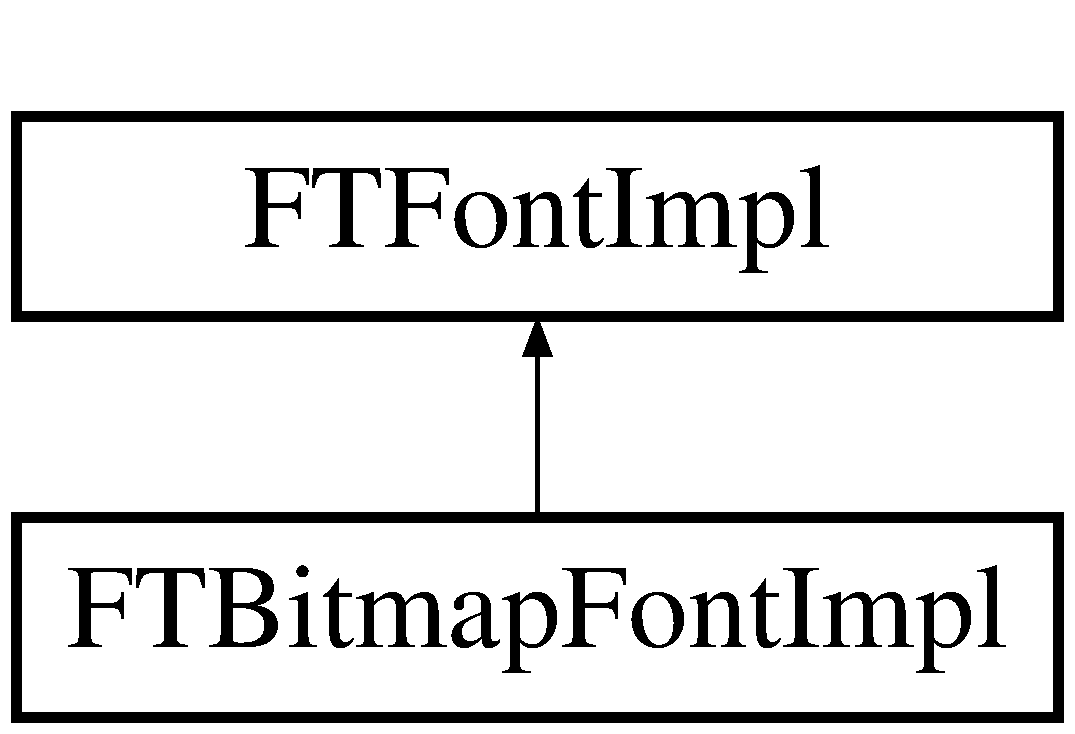
\includegraphics[height=2.000000cm]{class_f_t_bitmap_font_impl}
\end{center}
\end{figure}
\subsection*{Protected Member Functions}
\begin{DoxyCompactItemize}
\item 
\hypertarget{class_f_t_bitmap_font_impl_a8b9cc194fe4de235bca414dc0ffe0960}{
{\bfseries FTBitmapFontImpl} (FTFont $\ast$ftFont, const char $\ast$fontFilePath)}
\label{class_f_t_bitmap_font_impl_a8b9cc194fe4de235bca414dc0ffe0960}

\item 
\hypertarget{class_f_t_bitmap_font_impl_ae066b9bf998e13a225be35767c25d233}{
{\bfseries FTBitmapFontImpl} (FTFont $\ast$ftFont, const unsigned char $\ast$pBufferBytes, size\_\-t bufferSizeInBytes)}
\label{class_f_t_bitmap_font_impl_ae066b9bf998e13a225be35767c25d233}

\item 
\hypertarget{class_f_t_bitmap_font_impl_abfea575dee2b6436bd8522be490f5715}{
virtual FTPoint {\bfseries Render} (const char $\ast$s, const int len, FTPoint position, FTPoint spacing, int renderMode)}
\label{class_f_t_bitmap_font_impl_abfea575dee2b6436bd8522be490f5715}

\item 
\hypertarget{class_f_t_bitmap_font_impl_aee25e8971e53c7f2f2946abe87a51161}{
virtual FTPoint {\bfseries Render} (const wchar\_\-t $\ast$s, const int len, FTPoint position, FTPoint spacing, int renderMode)}
\label{class_f_t_bitmap_font_impl_aee25e8971e53c7f2f2946abe87a51161}

\end{DoxyCompactItemize}
\subsection*{Friends}
\begin{DoxyCompactItemize}
\item 
\hypertarget{class_f_t_bitmap_font_impl_a7ba5a198d501799828a37b4b808b9352}{
class {\bfseries FTBitmapFont}}
\label{class_f_t_bitmap_font_impl_a7ba5a198d501799828a37b4b808b9352}

\end{DoxyCompactItemize}


The documentation for this class was generated from the following files:\begin{DoxyCompactItemize}
\item 
src/libs/FTGL/FTFont/FTBitmapFontImpl.h\item 
src/libs/FTGL/FTFont/FTBitmapFont.cpp\end{DoxyCompactItemize}

\hypertarget{class_f_t_bitmap_glyph_impl}{
\section{FTBitmapGlyphImpl Class Reference}
\label{class_f_t_bitmap_glyph_impl}\index{FTBitmapGlyphImpl@{FTBitmapGlyphImpl}}
}
Inheritance diagram for FTBitmapGlyphImpl:\begin{figure}[H]
\begin{center}
\leavevmode
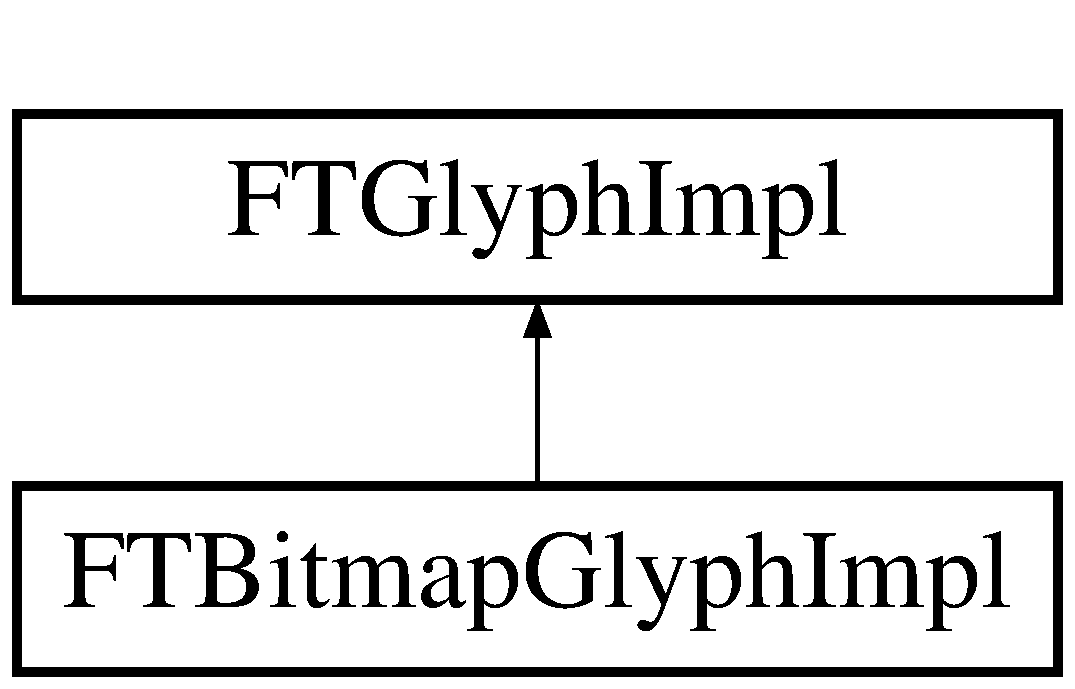
\includegraphics[height=2.000000cm]{class_f_t_bitmap_glyph_impl}
\end{center}
\end{figure}
\subsection*{Protected Member Functions}
\begin{DoxyCompactItemize}
\item 
\hypertarget{class_f_t_bitmap_glyph_impl_a4462585cd1fc2e461ff8c6a0b49c68b3}{
{\bfseries FTBitmapGlyphImpl} (\hyperlink{struct_f_t___glyph_slot_rec__}{FT\_\-GlyphSlot} glyph)}
\label{class_f_t_bitmap_glyph_impl_a4462585cd1fc2e461ff8c6a0b49c68b3}

\item 
\hypertarget{class_f_t_bitmap_glyph_impl_a31a412b09a68489ab2e96ad4524badde}{
virtual const FTPoint \& {\bfseries RenderImpl} (const FTPoint \&pen, int renderMode)}
\label{class_f_t_bitmap_glyph_impl_a31a412b09a68489ab2e96ad4524badde}

\end{DoxyCompactItemize}
\subsection*{Friends}
\begin{DoxyCompactItemize}
\item 
\hypertarget{class_f_t_bitmap_glyph_impl_aa3f0c28a7cfbfa0e896973476f7ed49d}{
class {\bfseries FTBitmapGlyph}}
\label{class_f_t_bitmap_glyph_impl_aa3f0c28a7cfbfa0e896973476f7ed49d}

\end{DoxyCompactItemize}


The documentation for this class was generated from the following files:\begin{DoxyCompactItemize}
\item 
src/libs/FTGL/FTGlyph/FTBitmapGlyphImpl.h\item 
src/libs/FTGL/FTGlyph/FTBitmapGlyph.cpp\end{DoxyCompactItemize}

\hypertarget{class_f_t_buffer_font_impl}{
\section{FTBufferFontImpl Class Reference}
\label{class_f_t_buffer_font_impl}\index{FTBufferFontImpl@{FTBufferFontImpl}}
}
Inheritance diagram for FTBufferFontImpl:\begin{figure}[H]
\begin{center}
\leavevmode
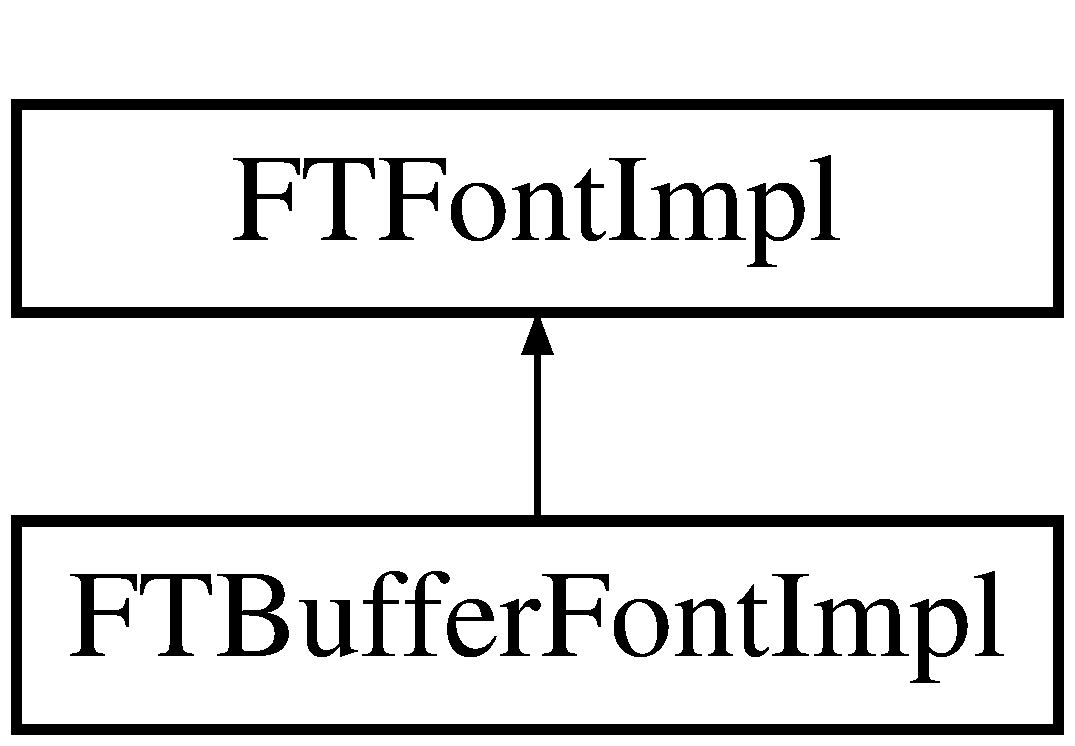
\includegraphics[height=2.000000cm]{class_f_t_buffer_font_impl}
\end{center}
\end{figure}
\subsection*{Protected Member Functions}
\begin{DoxyCompactItemize}
\item 
\hypertarget{class_f_t_buffer_font_impl_a968353f8f7e3fb37c0b1facd70599568}{
{\bfseries FTBufferFontImpl} (FTFont $\ast$ftFont, const char $\ast$fontFilePath)}
\label{class_f_t_buffer_font_impl_a968353f8f7e3fb37c0b1facd70599568}

\item 
\hypertarget{class_f_t_buffer_font_impl_a789d9507754a9e179d200fcf93690081}{
{\bfseries FTBufferFontImpl} (FTFont $\ast$ftFont, const unsigned char $\ast$pBufferBytes, size\_\-t bufferSizeInBytes)}
\label{class_f_t_buffer_font_impl_a789d9507754a9e179d200fcf93690081}

\item 
\hypertarget{class_f_t_buffer_font_impl_a82fccb46df5d5b17f654d23773faa8ae}{
virtual FTPoint {\bfseries Render} (const char $\ast$s, const int len, FTPoint position, FTPoint spacing, int renderMode)}
\label{class_f_t_buffer_font_impl_a82fccb46df5d5b17f654d23773faa8ae}

\item 
\hypertarget{class_f_t_buffer_font_impl_ad56722bcd6030ee1cae56c307b254ec1}{
virtual FTPoint {\bfseries Render} (const wchar\_\-t $\ast$s, const int len, FTPoint position, FTPoint spacing, int renderMode)}
\label{class_f_t_buffer_font_impl_ad56722bcd6030ee1cae56c307b254ec1}

\item 
\hypertarget{class_f_t_buffer_font_impl_a4bd13aeb53fc5585d91546095c389868}{
virtual bool {\bfseries FaceSize} (const unsigned int size, const unsigned int res)}
\label{class_f_t_buffer_font_impl_a4bd13aeb53fc5585d91546095c389868}

\end{DoxyCompactItemize}
\subsection*{Friends}
\begin{DoxyCompactItemize}
\item 
\hypertarget{class_f_t_buffer_font_impl_ab7dc21f40be33fee50c41b3ba3d49c73}{
class {\bfseries FTBufferFont}}
\label{class_f_t_buffer_font_impl_ab7dc21f40be33fee50c41b3ba3d49c73}

\end{DoxyCompactItemize}


The documentation for this class was generated from the following files:\begin{DoxyCompactItemize}
\item 
src/libs/FTGL/FTFont/FTBufferFontImpl.h\item 
src/libs/FTGL/FTFont/FTBufferFont.cpp\end{DoxyCompactItemize}

\hypertarget{class_f_t_buffer_glyph_impl}{
\section{FTBufferGlyphImpl Class Reference}
\label{class_f_t_buffer_glyph_impl}\index{FTBufferGlyphImpl@{FTBufferGlyphImpl}}
}
Inheritance diagram for FTBufferGlyphImpl:\begin{figure}[H]
\begin{center}
\leavevmode
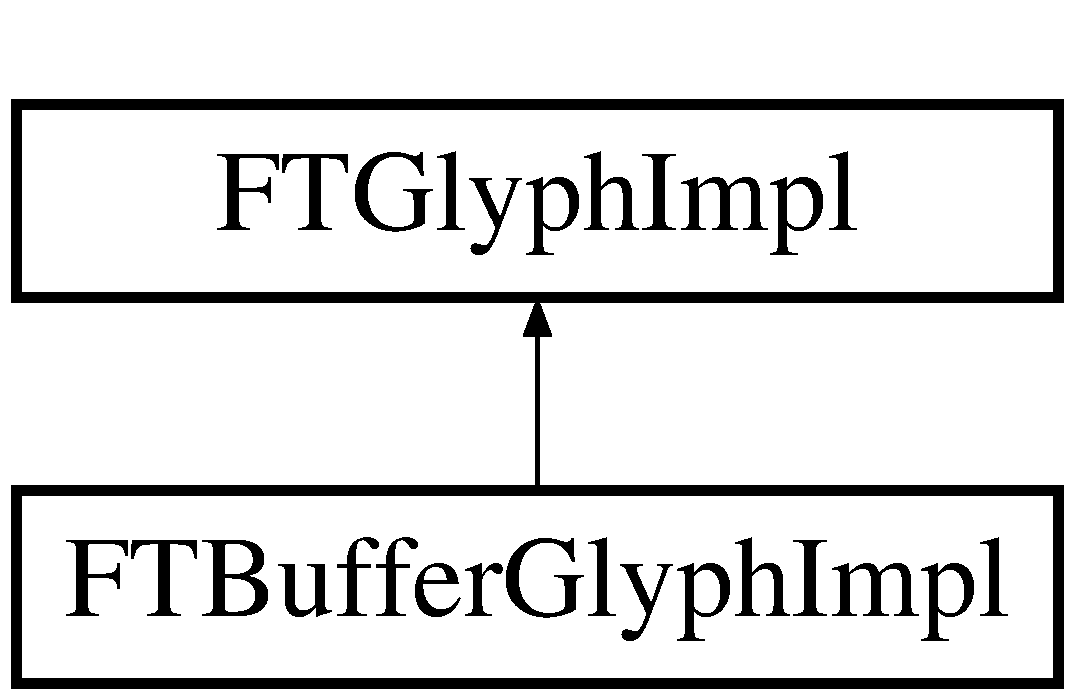
\includegraphics[height=2.000000cm]{class_f_t_buffer_glyph_impl}
\end{center}
\end{figure}
\subsection*{Protected Member Functions}
\begin{DoxyCompactItemize}
\item 
\hypertarget{class_f_t_buffer_glyph_impl_a02a187494995d95792ef66767f04c56d}{
{\bfseries FTBufferGlyphImpl} (\hyperlink{struct_f_t___glyph_slot_rec__}{FT\_\-GlyphSlot} glyph, FTBuffer $\ast$p)}
\label{class_f_t_buffer_glyph_impl_a02a187494995d95792ef66767f04c56d}

\item 
\hypertarget{class_f_t_buffer_glyph_impl_a4f7f56caf34309cf7e1408a631b419de}{
virtual const FTPoint \& {\bfseries RenderImpl} (const FTPoint \&pen, int renderMode)}
\label{class_f_t_buffer_glyph_impl_a4f7f56caf34309cf7e1408a631b419de}

\end{DoxyCompactItemize}
\subsection*{Friends}
\begin{DoxyCompactItemize}
\item 
\hypertarget{class_f_t_buffer_glyph_impl_a385e2288042fd77f037a715e7801b451}{
class {\bfseries FTBufferGlyph}}
\label{class_f_t_buffer_glyph_impl_a385e2288042fd77f037a715e7801b451}

\end{DoxyCompactItemize}


The documentation for this class was generated from the following files:\begin{DoxyCompactItemize}
\item 
src/libs/FTGL/FTGlyph/FTBufferGlyphImpl.h\item 
src/libs/FTGL/FTGlyph/FTBufferGlyph.cpp\end{DoxyCompactItemize}

\hypertarget{struct_f_t_c___image_type_rec__}{
\section{FTC\_\-ImageTypeRec\_\- Struct Reference}
\label{struct_f_t_c___image_type_rec__}\index{FTC\_\-ImageTypeRec\_\-@{FTC\_\-ImageTypeRec\_\-}}
}
\subsection*{Public Attributes}
\begin{DoxyCompactItemize}
\item 
\hypertarget{struct_f_t_c___image_type_rec___a9851b8d4a06baacd18d5b9856fd85abd}{
FTC\_\-FaceID {\bfseries face\_\-id}}
\label{struct_f_t_c___image_type_rec___a9851b8d4a06baacd18d5b9856fd85abd}

\item 
\hypertarget{struct_f_t_c___image_type_rec___af1a4cccbabb0f5852ed755a12ed08dd8}{
FT\_\-Int {\bfseries width}}
\label{struct_f_t_c___image_type_rec___af1a4cccbabb0f5852ed755a12ed08dd8}

\item 
\hypertarget{struct_f_t_c___image_type_rec___adb56a9d18a3f522d713d0ba01c1a8778}{
FT\_\-Int {\bfseries height}}
\label{struct_f_t_c___image_type_rec___adb56a9d18a3f522d713d0ba01c1a8778}

\item 
\hypertarget{struct_f_t_c___image_type_rec___a391782ed8c67de86591c71f276ea6454}{
FT\_\-Int32 {\bfseries flags}}
\label{struct_f_t_c___image_type_rec___a391782ed8c67de86591c71f276ea6454}

\end{DoxyCompactItemize}


The documentation for this struct was generated from the following file:\begin{DoxyCompactItemize}
\item 
src/libs/freetype/ftcache.h\end{DoxyCompactItemize}

\hypertarget{struct_f_t_c___s_bit_rec__}{
\section{FTC\_\-SBitRec\_\- Struct Reference}
\label{struct_f_t_c___s_bit_rec__}\index{FTC\_\-SBitRec\_\-@{FTC\_\-SBitRec\_\-}}
}
\subsection*{Public Attributes}
\begin{DoxyCompactItemize}
\item 
\hypertarget{struct_f_t_c___s_bit_rec___a5b92fb4f213a880f758bb87ac2ceb263}{
FT\_\-Byte {\bfseries width}}
\label{struct_f_t_c___s_bit_rec___a5b92fb4f213a880f758bb87ac2ceb263}

\item 
\hypertarget{struct_f_t_c___s_bit_rec___a5953efe2aded3b184875d5e5d08cafef}{
FT\_\-Byte {\bfseries height}}
\label{struct_f_t_c___s_bit_rec___a5953efe2aded3b184875d5e5d08cafef}

\item 
\hypertarget{struct_f_t_c___s_bit_rec___aef273749f4fdb9943500ec6df8412a94}{
FT\_\-Char {\bfseries left}}
\label{struct_f_t_c___s_bit_rec___aef273749f4fdb9943500ec6df8412a94}

\item 
\hypertarget{struct_f_t_c___s_bit_rec___a3e558b3a04b70f00f80b862cdc94d9a2}{
FT\_\-Char {\bfseries top}}
\label{struct_f_t_c___s_bit_rec___a3e558b3a04b70f00f80b862cdc94d9a2}

\item 
\hypertarget{struct_f_t_c___s_bit_rec___a3d3fcc2869ce5c95f0f63898e6cef8be}{
FT\_\-Byte {\bfseries format}}
\label{struct_f_t_c___s_bit_rec___a3d3fcc2869ce5c95f0f63898e6cef8be}

\item 
\hypertarget{struct_f_t_c___s_bit_rec___a83958d4649a898312de9a7274550dff9}{
FT\_\-Byte {\bfseries max\_\-grays}}
\label{struct_f_t_c___s_bit_rec___a83958d4649a898312de9a7274550dff9}

\item 
\hypertarget{struct_f_t_c___s_bit_rec___a1382ec014df599e706c2c1785bc18235}{
FT\_\-Short {\bfseries pitch}}
\label{struct_f_t_c___s_bit_rec___a1382ec014df599e706c2c1785bc18235}

\item 
\hypertarget{struct_f_t_c___s_bit_rec___a502a0bb69d973d2ae626a842eb9fefd3}{
FT\_\-Char {\bfseries xadvance}}
\label{struct_f_t_c___s_bit_rec___a502a0bb69d973d2ae626a842eb9fefd3}

\item 
\hypertarget{struct_f_t_c___s_bit_rec___aabe767ddaf7ff62918886c6f62e9ac28}{
FT\_\-Char {\bfseries yadvance}}
\label{struct_f_t_c___s_bit_rec___aabe767ddaf7ff62918886c6f62e9ac28}

\item 
\hypertarget{struct_f_t_c___s_bit_rec___abe4d78fc3f411d67e7fc43f7aa21bd1d}{
FT\_\-Byte $\ast$ {\bfseries buffer}}
\label{struct_f_t_c___s_bit_rec___abe4d78fc3f411d67e7fc43f7aa21bd1d}

\end{DoxyCompactItemize}


The documentation for this struct was generated from the following file:\begin{DoxyCompactItemize}
\item 
src/libs/freetype/ftcache.h\end{DoxyCompactItemize}

\hypertarget{struct_f_t_c___scaler_rec__}{
\section{FTC\_\-ScalerRec\_\- Struct Reference}
\label{struct_f_t_c___scaler_rec__}\index{FTC\_\-ScalerRec\_\-@{FTC\_\-ScalerRec\_\-}}
}
\subsection*{Public Attributes}
\begin{DoxyCompactItemize}
\item 
\hypertarget{struct_f_t_c___scaler_rec___a8e963aa619409e646558fe7aa272e81f}{
FTC\_\-FaceID {\bfseries face\_\-id}}
\label{struct_f_t_c___scaler_rec___a8e963aa619409e646558fe7aa272e81f}

\item 
\hypertarget{struct_f_t_c___scaler_rec___a11e13d907ca4661bf7c1d98fffecf321}{
FT\_\-UInt {\bfseries width}}
\label{struct_f_t_c___scaler_rec___a11e13d907ca4661bf7c1d98fffecf321}

\item 
\hypertarget{struct_f_t_c___scaler_rec___a9b3a9b4d7148bbaa4daaae1e1fbb2dbc}{
FT\_\-UInt {\bfseries height}}
\label{struct_f_t_c___scaler_rec___a9b3a9b4d7148bbaa4daaae1e1fbb2dbc}

\item 
\hypertarget{struct_f_t_c___scaler_rec___ab78868341e2d66f17e6f1d77e9e054d2}{
FT\_\-Int {\bfseries pixel}}
\label{struct_f_t_c___scaler_rec___ab78868341e2d66f17e6f1d77e9e054d2}

\item 
\hypertarget{struct_f_t_c___scaler_rec___a886c7c1230dc5d5e6b3fc32d06274752}{
FT\_\-UInt {\bfseries x\_\-res}}
\label{struct_f_t_c___scaler_rec___a886c7c1230dc5d5e6b3fc32d06274752}

\item 
\hypertarget{struct_f_t_c___scaler_rec___accb53c7a9aeebb41c05f48d14d3dfe71}{
FT\_\-UInt {\bfseries y\_\-res}}
\label{struct_f_t_c___scaler_rec___accb53c7a9aeebb41c05f48d14d3dfe71}

\end{DoxyCompactItemize}


The documentation for this struct was generated from the following file:\begin{DoxyCompactItemize}
\item 
src/libs/freetype/ftcache.h\end{DoxyCompactItemize}

\hypertarget{class_f_t_charmap}{
\section{FTCharmap Class Reference}
\label{class_f_t_charmap}\index{FTCharmap@{FTCharmap}}
}
\subsection*{Public Member Functions}
\begin{DoxyCompactItemize}
\item 
\hyperlink{class_f_t_charmap_a9d19837becbc83acf7f56a5980b2b644}{FTCharmap} (\hyperlink{class_f_t_face}{FTFace} $\ast$face)
\item 
virtual \hyperlink{class_f_t_charmap_afcbe1e49ed38810e8b9c2e116ddbbffc}{$\sim$FTCharmap} ()
\item 
FT\_\-Encoding \hyperlink{class_f_t_charmap_a4c119ad30110e00b6b3944288a702c84}{Encoding} () const 
\item 
bool \hyperlink{class_f_t_charmap_a4d182b0faeb7198b4f583b84eaf4cd55}{CharMap} (FT\_\-Encoding encoding)
\item 
unsigned int \hyperlink{class_f_t_charmap_a6084cc8ab267b9974980e14f17227f25}{GlyphListIndex} (const unsigned int characterCode)
\item 
unsigned int \hyperlink{class_f_t_charmap_ab77d9f06a9109608b1734010acecaefd}{FontIndex} (const unsigned int characterCode)
\item 
void \hyperlink{class_f_t_charmap_a374e41b6f8b07efb08e5c173cc707354}{InsertIndex} (const unsigned int characterCode, const size\_\-t containerIndex)
\item 
FT\_\-Error \hyperlink{class_f_t_charmap_a176e217e3e837db5fc4592ceff5ed488}{Error} () const 
\end{DoxyCompactItemize}


\subsection{Constructor \& Destructor Documentation}
\hypertarget{class_f_t_charmap_a9d19837becbc83acf7f56a5980b2b644}{
\index{FTCharmap@{FTCharmap}!FTCharmap@{FTCharmap}}
\index{FTCharmap@{FTCharmap}!FTCharmap@{FTCharmap}}
\subsubsection[{FTCharmap}]{\setlength{\rightskip}{0pt plus 5cm}FTCharmap::FTCharmap (
\begin{DoxyParamCaption}
\item[{{\bf FTFace} $\ast$}]{ face}
\end{DoxyParamCaption}
)}}
\label{class_f_t_charmap_a9d19837becbc83acf7f56a5980b2b644}
Constructor \hypertarget{class_f_t_charmap_afcbe1e49ed38810e8b9c2e116ddbbffc}{
\index{FTCharmap@{FTCharmap}!$\sim$FTCharmap@{$\sim$FTCharmap}}
\index{$\sim$FTCharmap@{$\sim$FTCharmap}!FTCharmap@{FTCharmap}}
\subsubsection[{$\sim$FTCharmap}]{\setlength{\rightskip}{0pt plus 5cm}FTCharmap::$\sim$FTCharmap (
\begin{DoxyParamCaption}
{}
\end{DoxyParamCaption}
)\hspace{0.3cm}{\ttfamily  \mbox{[}virtual\mbox{]}}}}
\label{class_f_t_charmap_afcbe1e49ed38810e8b9c2e116ddbbffc}
Destructor 

\subsection{Member Function Documentation}
\hypertarget{class_f_t_charmap_a4d182b0faeb7198b4f583b84eaf4cd55}{
\index{FTCharmap@{FTCharmap}!CharMap@{CharMap}}
\index{CharMap@{CharMap}!FTCharmap@{FTCharmap}}
\subsubsection[{CharMap}]{\setlength{\rightskip}{0pt plus 5cm}bool FTCharmap::CharMap (
\begin{DoxyParamCaption}
\item[{FT\_\-Encoding}]{ encoding}
\end{DoxyParamCaption}
)}}
\label{class_f_t_charmap_a4d182b0faeb7198b4f583b84eaf4cd55}
Sets the character map for the face. If an error occurs the object is not modified. Valid encodings as at Freetype 2.0.4 ft\_\-encoding\_\-none ft\_\-encoding\_\-symbol ft\_\-encoding\_\-unicode ft\_\-encoding\_\-latin\_\-2 ft\_\-encoding\_\-sjis ft\_\-encoding\_\-gb2312 ft\_\-encoding\_\-big5 ft\_\-encoding\_\-wansung ft\_\-encoding\_\-johab ft\_\-encoding\_\-adobe\_\-standard ft\_\-encoding\_\-adobe\_\-expert ft\_\-encoding\_\-adobe\_\-custom ft\_\-encoding\_\-apple\_\-roman


\begin{DoxyParams}{Parameters}
{\em encoding} & the Freetype encoding symbol. See above. \\
\hline
\end{DoxyParams}
\begin{DoxyReturn}{Returns}
{\ttfamily true} if charmap was valid and set correctly. 
\end{DoxyReturn}
\hypertarget{class_f_t_charmap_a4c119ad30110e00b6b3944288a702c84}{
\index{FTCharmap@{FTCharmap}!Encoding@{Encoding}}
\index{Encoding@{Encoding}!FTCharmap@{FTCharmap}}
\subsubsection[{Encoding}]{\setlength{\rightskip}{0pt plus 5cm}FT\_\-Encoding FTCharmap::Encoding (
\begin{DoxyParamCaption}
{}
\end{DoxyParamCaption}
) const\hspace{0.3cm}{\ttfamily  \mbox{[}inline\mbox{]}}}}
\label{class_f_t_charmap_a4c119ad30110e00b6b3944288a702c84}
Queries for the current character map code.

\begin{DoxyReturn}{Returns}
The current character map code. 
\end{DoxyReturn}
\hypertarget{class_f_t_charmap_a176e217e3e837db5fc4592ceff5ed488}{
\index{FTCharmap@{FTCharmap}!Error@{Error}}
\index{Error@{Error}!FTCharmap@{FTCharmap}}
\subsubsection[{Error}]{\setlength{\rightskip}{0pt plus 5cm}FT\_\-Error FTCharmap::Error (
\begin{DoxyParamCaption}
{}
\end{DoxyParamCaption}
) const\hspace{0.3cm}{\ttfamily  \mbox{[}inline\mbox{]}}}}
\label{class_f_t_charmap_a176e217e3e837db5fc4592ceff5ed488}
Queries for errors.

\begin{DoxyReturn}{Returns}
The current error code. Zero means no error. 
\end{DoxyReturn}
\hypertarget{class_f_t_charmap_ab77d9f06a9109608b1734010acecaefd}{
\index{FTCharmap@{FTCharmap}!FontIndex@{FontIndex}}
\index{FontIndex@{FontIndex}!FTCharmap@{FTCharmap}}
\subsubsection[{FontIndex}]{\setlength{\rightskip}{0pt plus 5cm}unsigned int FTCharmap::FontIndex (
\begin{DoxyParamCaption}
\item[{const unsigned int}]{ characterCode}
\end{DoxyParamCaption}
)}}
\label{class_f_t_charmap_ab77d9f06a9109608b1734010acecaefd}
Get the font glyph index of the input character.


\begin{DoxyParams}{Parameters}
{\em characterCode} & The character code of the requested glyph in the current encoding eg apple roman. \\
\hline
\end{DoxyParams}
\begin{DoxyReturn}{Returns}
The glyph index for the character. 
\end{DoxyReturn}
\hypertarget{class_f_t_charmap_a6084cc8ab267b9974980e14f17227f25}{
\index{FTCharmap@{FTCharmap}!GlyphListIndex@{GlyphListIndex}}
\index{GlyphListIndex@{GlyphListIndex}!FTCharmap@{FTCharmap}}
\subsubsection[{GlyphListIndex}]{\setlength{\rightskip}{0pt plus 5cm}unsigned int FTCharmap::GlyphListIndex (
\begin{DoxyParamCaption}
\item[{const unsigned int}]{ characterCode}
\end{DoxyParamCaption}
)}}
\label{class_f_t_charmap_a6084cc8ab267b9974980e14f17227f25}
Get the \hyperlink{class_f_t_glyph_container}{FTGlyphContainer} index of the input character.


\begin{DoxyParams}{Parameters}
{\em characterCode} & The character code of the requested glyph in the current encoding eg apple roman. \\
\hline
\end{DoxyParams}
\begin{DoxyReturn}{Returns}
The \hyperlink{class_f_t_glyph_container}{FTGlyphContainer} index for the character or zero if it wasn't found 
\end{DoxyReturn}
\hypertarget{class_f_t_charmap_a374e41b6f8b07efb08e5c173cc707354}{
\index{FTCharmap@{FTCharmap}!InsertIndex@{InsertIndex}}
\index{InsertIndex@{InsertIndex}!FTCharmap@{FTCharmap}}
\subsubsection[{InsertIndex}]{\setlength{\rightskip}{0pt plus 5cm}void FTCharmap::InsertIndex (
\begin{DoxyParamCaption}
\item[{const unsigned int}]{ characterCode, }
\item[{const size\_\-t}]{ containerIndex}
\end{DoxyParamCaption}
)}}
\label{class_f_t_charmap_a374e41b6f8b07efb08e5c173cc707354}
Set the \hyperlink{class_f_t_glyph_container}{FTGlyphContainer} index of the character code.


\begin{DoxyParams}{Parameters}
{\em characterCode} & The character code of the requested glyph in the current encoding eg apple roman. \\
\hline
{\em containerIndex} & The index into the \hyperlink{class_f_t_glyph_container}{FTGlyphContainer} of the character code. \\
\hline
\end{DoxyParams}


The documentation for this class was generated from the following files:\begin{DoxyCompactItemize}
\item 
src/libs/FTGL/FTCharmap.h\item 
src/libs/FTGL/FTCharmap.cpp\end{DoxyCompactItemize}

\hypertarget{class_f_t_char_to_glyph_index_map}{
\section{FTCharToGlyphIndexMap Class Reference}
\label{class_f_t_char_to_glyph_index_map}\index{FTCharToGlyphIndexMap@{FTCharToGlyphIndexMap}}
}


{\ttfamily \#include $<$FTCharToGlyphIndexMap.h$>$}

\subsection*{Public Types}
\begin{DoxyCompactItemize}
\item 
enum \{ {\bfseries NumberOfBuckets} =  256, 
{\bfseries BucketSize} =  256, 
{\bfseries IndexNotFound} =  -\/1
 \}
\item 
\hypertarget{class_f_t_char_to_glyph_index_map_a0c3d673d5c3e978b7c04ea367f82e624}{
typedef unsigned long {\bfseries CharacterCode}}
\label{class_f_t_char_to_glyph_index_map_a0c3d673d5c3e978b7c04ea367f82e624}

\item 
\hypertarget{class_f_t_char_to_glyph_index_map_a54a7eca7f7b06f9389c12ab96db36a25}{
typedef signed long {\bfseries GlyphIndex}}
\label{class_f_t_char_to_glyph_index_map_a54a7eca7f7b06f9389c12ab96db36a25}

\end{DoxyCompactItemize}
\subsection*{Public Member Functions}
\begin{DoxyCompactItemize}
\item 
\hypertarget{class_f_t_char_to_glyph_index_map_adc045f0ce5b32fa84681d63e35ac7369}{
void {\bfseries clear} ()}
\label{class_f_t_char_to_glyph_index_map_adc045f0ce5b32fa84681d63e35ac7369}

\item 
\hypertarget{class_f_t_char_to_glyph_index_map_a94a2e63c8689298ac8dffdc90f290bb2}{
const GlyphIndex {\bfseries find} (CharacterCode c)}
\label{class_f_t_char_to_glyph_index_map_a94a2e63c8689298ac8dffdc90f290bb2}

\item 
\hypertarget{class_f_t_char_to_glyph_index_map_aa5ee6e5371094dfa05fa69145c33547f}{
void {\bfseries insert} (CharacterCode c, GlyphIndex g)}
\label{class_f_t_char_to_glyph_index_map_aa5ee6e5371094dfa05fa69145c33547f}

\end{DoxyCompactItemize}


\subsection{Detailed Description}
Provides a non-\/STL alternative to the STL map$<$unsigned long, unsigned long$>$ which maps character codes to glyph indices inside \hyperlink{class_f_t_charmap}{FTCharmap}.

Implementation:
\begin{DoxyItemize}
\item NumberOfBuckets buckets are considered.
\item Each bucket has BucketSize entries.
\item When the glyph index for the character code C has to be stored, the bucket this character belongs to is found using 'C div BucketSize'. If this bucket has not been allocated yet, do it now. The entry in the bucked is found using 'C mod BucketSize'. If it is set to IndexNotFound, then the glyph entry has not been set.
\item Try to mimic the calls made to the STL map API.
\end{DoxyItemize}

Caveats:
\begin{DoxyItemize}
\item The glyph index is now a signed long instead of unsigned long, so the special value IndexNotFound (= -\/1) can be used to specify that the glyph index has not been stored yet. 
\end{DoxyItemize}

The documentation for this class was generated from the following file:\begin{DoxyCompactItemize}
\item 
src/libs/FTGL/FTCharToGlyphIndexMap.h\end{DoxyCompactItemize}

\hypertarget{class_f_t_contour}{
\section{FTContour Class Reference}
\label{class_f_t_contour}\index{FTContour@{FTContour}}
}


{\ttfamily \#include $<$FTContour.h$>$}

\subsection*{Public Member Functions}
\begin{DoxyCompactItemize}
\item 
\hyperlink{class_f_t_contour_a1a682c070617bf9023ea38c65b32ade3}{FTContour} (\hyperlink{struct_f_t___vector__}{FT\_\-Vector} $\ast$contour, char $\ast$pointTags, unsigned int numberOfPoints)
\item 
\hyperlink{class_f_t_contour_a89ac638fc2bbe641d730af84bf13b242}{$\sim$FTContour} ()
\item 
const FTPoint \& \hyperlink{class_f_t_contour_a055f10124231687d7647d56ee6b680ef}{Point} (size\_\-t index) const 
\item 
const FTPoint \& \hyperlink{class_f_t_contour_a5b720df9b54e3564d762a6fe8eee3143}{Outset} (size\_\-t index) const 
\item 
const FTPoint \& \hyperlink{class_f_t_contour_a89f7120855b97ae91c63d13cd22f3e04}{FrontPoint} (size\_\-t index) const 
\item 
const FTPoint \& \hyperlink{class_f_t_contour_add4587cac25790725e704fdd7e9fa9fe}{BackPoint} (size\_\-t index) const 
\item 
size\_\-t \hyperlink{class_f_t_contour_ab31ce24e66d9534b5e0b052b0b6f408b}{PointCount} () const 
\item 
void \hyperlink{class_f_t_contour_a7129afbf6bde74d5c9c46ad47bf6e049}{SetParity} (int parity)
\item 
\hypertarget{class_f_t_contour_ab91b659e8de1dc915679d0152adfa38a}{
void {\bfseries buildFrontOutset} (float outset)}
\label{class_f_t_contour_ab91b659e8de1dc915679d0152adfa38a}

\item 
\hypertarget{class_f_t_contour_aff16d21542506b738c7f883b7c40b738}{
void {\bfseries buildBackOutset} (float outset)}
\label{class_f_t_contour_aff16d21542506b738c7f883b7c40b738}

\end{DoxyCompactItemize}


\subsection{Detailed Description}
\hyperlink{class_f_t_contour}{FTContour} class is a container of points that describe a vector font outline. It is used as a container for the output of the bezier curve evaluator in \hyperlink{class_f_t_vectoriser}{FTVectoriser}.

\begin{DoxySeeAlso}{See also}
FTOutlineGlyph 

FTPolygonGlyph 

FTPoint 
\end{DoxySeeAlso}


\subsection{Constructor \& Destructor Documentation}
\hypertarget{class_f_t_contour_a1a682c070617bf9023ea38c65b32ade3}{
\index{FTContour@{FTContour}!FTContour@{FTContour}}
\index{FTContour@{FTContour}!FTContour@{FTContour}}
\subsubsection[{FTContour}]{\setlength{\rightskip}{0pt plus 5cm}FTContour::FTContour (
\begin{DoxyParamCaption}
\item[{{\bf FT\_\-Vector} $\ast$}]{ contour, }
\item[{char $\ast$}]{ pointTags, }
\item[{unsigned int}]{ numberOfPoints}
\end{DoxyParamCaption}
)}}
\label{class_f_t_contour_a1a682c070617bf9023ea38c65b32ade3}
Constructor


\begin{DoxyParams}{Parameters}
{\em contour} & \\
\hline
{\em pointTags} & \\
\hline
{\em numberOfPoints} & \\
\hline
\end{DoxyParams}
\hypertarget{class_f_t_contour_a89ac638fc2bbe641d730af84bf13b242}{
\index{FTContour@{FTContour}!$\sim$FTContour@{$\sim$FTContour}}
\index{$\sim$FTContour@{$\sim$FTContour}!FTContour@{FTContour}}
\subsubsection[{$\sim$FTContour}]{\setlength{\rightskip}{0pt plus 5cm}FTContour::$\sim$FTContour (
\begin{DoxyParamCaption}
{}
\end{DoxyParamCaption}
)\hspace{0.3cm}{\ttfamily  \mbox{[}inline\mbox{]}}}}
\label{class_f_t_contour_a89ac638fc2bbe641d730af84bf13b242}
Destructor 

\subsection{Member Function Documentation}
\hypertarget{class_f_t_contour_add4587cac25790725e704fdd7e9fa9fe}{
\index{FTContour@{FTContour}!BackPoint@{BackPoint}}
\index{BackPoint@{BackPoint}!FTContour@{FTContour}}
\subsubsection[{BackPoint}]{\setlength{\rightskip}{0pt plus 5cm}const FTPoint\& FTContour::BackPoint (
\begin{DoxyParamCaption}
\item[{size\_\-t}]{ index}
\end{DoxyParamCaption}
) const\hspace{0.3cm}{\ttfamily  \mbox{[}inline\mbox{]}}}}
\label{class_f_t_contour_add4587cac25790725e704fdd7e9fa9fe}
Return a point at index of the back outset contour.


\begin{DoxyParams}{Parameters}
{\em index} & of the point in the curve. \\
\hline
\end{DoxyParams}
\begin{DoxyReturn}{Returns}
const point reference 
\end{DoxyReturn}
\hypertarget{class_f_t_contour_a89f7120855b97ae91c63d13cd22f3e04}{
\index{FTContour@{FTContour}!FrontPoint@{FrontPoint}}
\index{FrontPoint@{FrontPoint}!FTContour@{FTContour}}
\subsubsection[{FrontPoint}]{\setlength{\rightskip}{0pt plus 5cm}const FTPoint\& FTContour::FrontPoint (
\begin{DoxyParamCaption}
\item[{size\_\-t}]{ index}
\end{DoxyParamCaption}
) const\hspace{0.3cm}{\ttfamily  \mbox{[}inline\mbox{]}}}}
\label{class_f_t_contour_a89f7120855b97ae91c63d13cd22f3e04}
Return a point at index of the front outset contour.


\begin{DoxyParams}{Parameters}
{\em index} & of the point in the curve. \\
\hline
\end{DoxyParams}
\begin{DoxyReturn}{Returns}
const point reference 
\end{DoxyReturn}
\hypertarget{class_f_t_contour_a5b720df9b54e3564d762a6fe8eee3143}{
\index{FTContour@{FTContour}!Outset@{Outset}}
\index{Outset@{Outset}!FTContour@{FTContour}}
\subsubsection[{Outset}]{\setlength{\rightskip}{0pt plus 5cm}const FTPoint\& FTContour::Outset (
\begin{DoxyParamCaption}
\item[{size\_\-t}]{ index}
\end{DoxyParamCaption}
) const\hspace{0.3cm}{\ttfamily  \mbox{[}inline\mbox{]}}}}
\label{class_f_t_contour_a5b720df9b54e3564d762a6fe8eee3143}
Return a point at index.


\begin{DoxyParams}{Parameters}
{\em index} & of the point in the outset curve. \\
\hline
\end{DoxyParams}
\begin{DoxyReturn}{Returns}
const point reference 
\end{DoxyReturn}
\hypertarget{class_f_t_contour_a055f10124231687d7647d56ee6b680ef}{
\index{FTContour@{FTContour}!Point@{Point}}
\index{Point@{Point}!FTContour@{FTContour}}
\subsubsection[{Point}]{\setlength{\rightskip}{0pt plus 5cm}const FTPoint\& FTContour::Point (
\begin{DoxyParamCaption}
\item[{size\_\-t}]{ index}
\end{DoxyParamCaption}
) const\hspace{0.3cm}{\ttfamily  \mbox{[}inline\mbox{]}}}}
\label{class_f_t_contour_a055f10124231687d7647d56ee6b680ef}
Return a point at index.


\begin{DoxyParams}{Parameters}
{\em index} & of the point in the curve. \\
\hline
\end{DoxyParams}
\begin{DoxyReturn}{Returns}
const point reference 
\end{DoxyReturn}
\hypertarget{class_f_t_contour_ab31ce24e66d9534b5e0b052b0b6f408b}{
\index{FTContour@{FTContour}!PointCount@{PointCount}}
\index{PointCount@{PointCount}!FTContour@{FTContour}}
\subsubsection[{PointCount}]{\setlength{\rightskip}{0pt plus 5cm}size\_\-t FTContour::PointCount (
\begin{DoxyParamCaption}
{}
\end{DoxyParamCaption}
) const\hspace{0.3cm}{\ttfamily  \mbox{[}inline\mbox{]}}}}
\label{class_f_t_contour_ab31ce24e66d9534b5e0b052b0b6f408b}
How many points define this contour

\begin{DoxyReturn}{Returns}
the number of points in this contour 
\end{DoxyReturn}
\hypertarget{class_f_t_contour_a7129afbf6bde74d5c9c46ad47bf6e049}{
\index{FTContour@{FTContour}!SetParity@{SetParity}}
\index{SetParity@{SetParity}!FTContour@{FTContour}}
\subsubsection[{SetParity}]{\setlength{\rightskip}{0pt plus 5cm}void FTContour::SetParity (
\begin{DoxyParamCaption}
\item[{int}]{ parity}
\end{DoxyParamCaption}
)}}
\label{class_f_t_contour_a7129afbf6bde74d5c9c46ad47bf6e049}
Make sure the glyph has the proper parity and create the front/back outset contour.


\begin{DoxyParams}{Parameters}
{\em parity} & The contour's parity within the glyph. \\
\hline
\end{DoxyParams}


The documentation for this class was generated from the following files:\begin{DoxyCompactItemize}
\item 
src/libs/FTGL/FTContour.h\item 
src/libs/FTGL/FTContour.cpp\end{DoxyCompactItemize}

\hypertarget{class_f_t_custom_font}{
\section{FTCustomFont Class Reference}
\label{class_f_t_custom_font}\index{FTCustomFont@{FTCustomFont}}
}
\subsection*{Public Member Functions}
\begin{DoxyCompactItemize}
\item 
\hypertarget{class_f_t_custom_font_a752e3adba12661605536402b55381aa8}{
{\bfseries FTCustomFont} (char const $\ast$fontFilePath, void $\ast$p, \hyperlink{struct___f_t_g_lglyph}{FTGLglyph} $\ast$($\ast$makeglyph)(\hyperlink{struct_f_t___glyph_slot_rec__}{FT\_\-GlyphSlot}, void $\ast$))}
\label{class_f_t_custom_font_a752e3adba12661605536402b55381aa8}

\item 
\hypertarget{class_f_t_custom_font_a14863f6c098d220681087ff85f004dff}{
FTGlyph $\ast$ {\bfseries MakeGlyph} (\hyperlink{struct_f_t___glyph_slot_rec__}{FT\_\-GlyphSlot} slot)}
\label{class_f_t_custom_font_a14863f6c098d220681087ff85f004dff}

\end{DoxyCompactItemize}


The documentation for this class was generated from the following file:\begin{DoxyCompactItemize}
\item 
src/libs/FTGL/FTFont/FTFontGlue.cpp\end{DoxyCompactItemize}

\hypertarget{class_f_t_custom_glyph}{
\section{FTCustomGlyph Class Reference}
\label{class_f_t_custom_glyph}\index{FTCustomGlyph@{FTCustomGlyph}}
}
\subsection*{Public Member Functions}
\begin{DoxyCompactItemize}
\item 
\hypertarget{class_f_t_custom_glyph_a43e4bfa9d8ccb5ae4d0e9c38cf7f01c1}{
{\bfseries FTCustomGlyph} (\hyperlink{struct___f_t_g_lglyph}{FTGLglyph} $\ast$base, void $\ast$p, void($\ast$render)(\hyperlink{struct___f_t_g_lglyph}{FTGLglyph} $\ast$, void $\ast$, FTGL\_\-DOUBLE, FTGL\_\-DOUBLE, int, FTGL\_\-DOUBLE $\ast$, FTGL\_\-DOUBLE $\ast$), void($\ast$destroy)(\hyperlink{struct___f_t_g_lglyph}{FTGLglyph} $\ast$, void $\ast$))}
\label{class_f_t_custom_glyph_a43e4bfa9d8ccb5ae4d0e9c38cf7f01c1}

\item 
\hypertarget{class_f_t_custom_glyph_aa8f17e3a9547eafed913e2b8f9b70958}{
float {\bfseries Advance} () const }
\label{class_f_t_custom_glyph_aa8f17e3a9547eafed913e2b8f9b70958}

\item 
\hypertarget{class_f_t_custom_glyph_a29285cf4a9b5476a80b01e1678272bd6}{
const FTPoint \& {\bfseries Render} (const FTPoint \&pen, int renderMode)}
\label{class_f_t_custom_glyph_a29285cf4a9b5476a80b01e1678272bd6}

\item 
\hypertarget{class_f_t_custom_glyph_aebed1d1515a24d6410f4c3f44686b75c}{
const FTBBox \& {\bfseries BBox} () const }
\label{class_f_t_custom_glyph_aebed1d1515a24d6410f4c3f44686b75c}

\item 
\hypertarget{class_f_t_custom_glyph_a8a74b76186fb02da48849c3c094fb72e}{
FT\_\-Error {\bfseries Error} () const }
\label{class_f_t_custom_glyph_a8a74b76186fb02da48849c3c094fb72e}

\end{DoxyCompactItemize}


The documentation for this class was generated from the following file:\begin{DoxyCompactItemize}
\item 
src/libs/FTGL/FTGlyph/FTGlyphGlue.cpp\end{DoxyCompactItemize}

\hypertarget{class_f_t_extrude_font_impl}{
\section{FTExtrudeFontImpl Class Reference}
\label{class_f_t_extrude_font_impl}\index{FTExtrudeFontImpl@{FTExtrudeFontImpl}}
}
Inheritance diagram for FTExtrudeFontImpl:\begin{figure}[H]
\begin{center}
\leavevmode
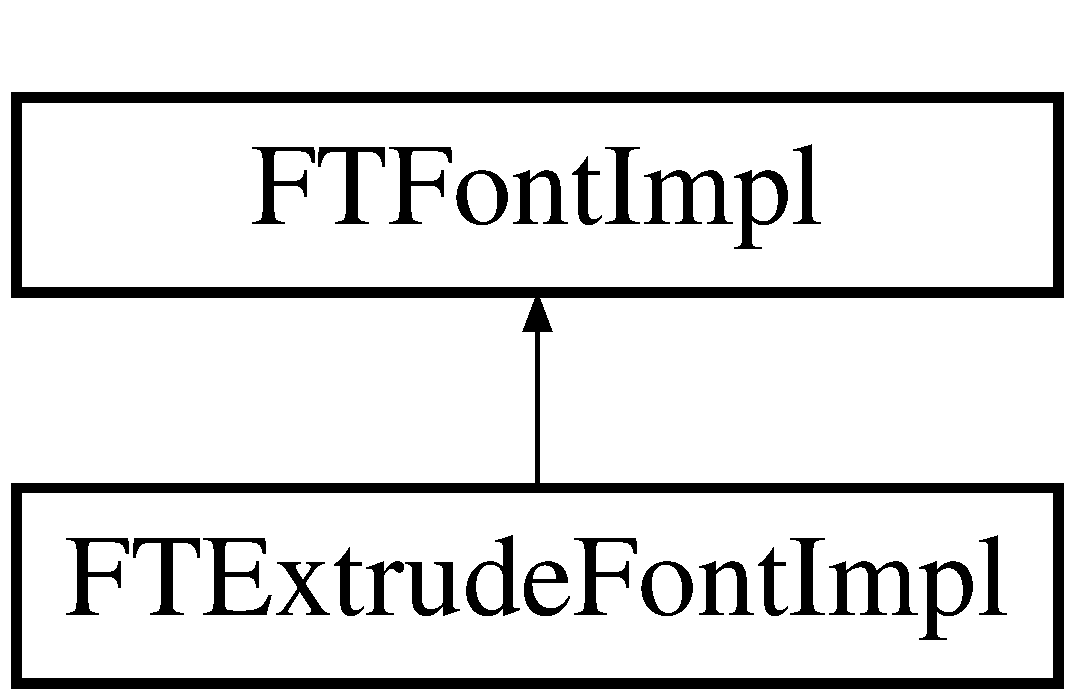
\includegraphics[height=2.000000cm]{class_f_t_extrude_font_impl}
\end{center}
\end{figure}
\subsection*{Protected Member Functions}
\begin{DoxyCompactItemize}
\item 
\hypertarget{class_f_t_extrude_font_impl_a43da54bf40a55db304395d8dec46897f}{
{\bfseries FTExtrudeFontImpl} (FTFont $\ast$ftFont, const char $\ast$fontFilePath)}
\label{class_f_t_extrude_font_impl_a43da54bf40a55db304395d8dec46897f}

\item 
\hypertarget{class_f_t_extrude_font_impl_aa433e0addf2dba2ae9232d6522ccdb5f}{
{\bfseries FTExtrudeFontImpl} (FTFont $\ast$ftFont, const unsigned char $\ast$pBufferBytes, size\_\-t bufferSizeInBytes)}
\label{class_f_t_extrude_font_impl_aa433e0addf2dba2ae9232d6522ccdb5f}

\item 
virtual void \hyperlink{class_f_t_extrude_font_impl_a852e6d263a34982d56d19dfdf43722f0}{Depth} (float d)
\item 
virtual void \hyperlink{class_f_t_extrude_font_impl_a559ce64b4d0e881455b050d3be57cac0}{Outset} (float o)
\item 
virtual void \hyperlink{class_f_t_extrude_font_impl_a24e6ada58e9086284e99611454c7b335}{Outset} (float f, float b)
\end{DoxyCompactItemize}
\subsection*{Friends}
\begin{DoxyCompactItemize}
\item 
\hypertarget{class_f_t_extrude_font_impl_a06be1600e211ee41aa1b1ed9c7d25639}{
class {\bfseries FTExtrudeFont}}
\label{class_f_t_extrude_font_impl_a06be1600e211ee41aa1b1ed9c7d25639}

\end{DoxyCompactItemize}


\subsection{Member Function Documentation}
\hypertarget{class_f_t_extrude_font_impl_a852e6d263a34982d56d19dfdf43722f0}{
\index{FTExtrudeFontImpl@{FTExtrudeFontImpl}!Depth@{Depth}}
\index{Depth@{Depth}!FTExtrudeFontImpl@{FTExtrudeFontImpl}}
\subsubsection[{Depth}]{\setlength{\rightskip}{0pt plus 5cm}virtual void FTExtrudeFontImpl::Depth (
\begin{DoxyParamCaption}
\item[{float}]{ d}
\end{DoxyParamCaption}
)\hspace{0.3cm}{\ttfamily  \mbox{[}inline, protected, virtual\mbox{]}}}}
\label{class_f_t_extrude_font_impl_a852e6d263a34982d56d19dfdf43722f0}
Set the extrusion distance for the font.


\begin{DoxyParams}{Parameters}
{\em d} & The extrusion distance. \\
\hline
\end{DoxyParams}


Reimplemented from \hyperlink{class_f_t_font_impl}{FTFontImpl}.

\hypertarget{class_f_t_extrude_font_impl_a24e6ada58e9086284e99611454c7b335}{
\index{FTExtrudeFontImpl@{FTExtrudeFontImpl}!Outset@{Outset}}
\index{Outset@{Outset}!FTExtrudeFontImpl@{FTExtrudeFontImpl}}
\subsubsection[{Outset}]{\setlength{\rightskip}{0pt plus 5cm}virtual void FTExtrudeFontImpl::Outset (
\begin{DoxyParamCaption}
\item[{float}]{ f, }
\item[{float}]{ b}
\end{DoxyParamCaption}
)\hspace{0.3cm}{\ttfamily  \mbox{[}inline, protected, virtual\mbox{]}}}}
\label{class_f_t_extrude_font_impl_a24e6ada58e9086284e99611454c7b335}
Set the outset distance for the font. Only implemented by FTExtrudeFont


\begin{DoxyParams}{Parameters}
{\em f} & The front outset distance. \\
\hline
{\em b} & The back outset distance. \\
\hline
\end{DoxyParams}


Reimplemented from \hyperlink{class_f_t_font_impl}{FTFontImpl}.

\hypertarget{class_f_t_extrude_font_impl_a559ce64b4d0e881455b050d3be57cac0}{
\index{FTExtrudeFontImpl@{FTExtrudeFontImpl}!Outset@{Outset}}
\index{Outset@{Outset}!FTExtrudeFontImpl@{FTExtrudeFontImpl}}
\subsubsection[{Outset}]{\setlength{\rightskip}{0pt plus 5cm}virtual void FTExtrudeFontImpl::Outset (
\begin{DoxyParamCaption}
\item[{float}]{ o}
\end{DoxyParamCaption}
)\hspace{0.3cm}{\ttfamily  \mbox{[}inline, protected, virtual\mbox{]}}}}
\label{class_f_t_extrude_font_impl_a559ce64b4d0e881455b050d3be57cac0}
Set the outset distance for the font. Only implemented by FTOutlineFont, FTPolygonFont and FTExtrudeFont


\begin{DoxyParams}{Parameters}
{\em o} & The outset distance. \\
\hline
\end{DoxyParams}


Reimplemented from \hyperlink{class_f_t_font_impl}{FTFontImpl}.



The documentation for this class was generated from the following files:\begin{DoxyCompactItemize}
\item 
src/libs/FTGL/FTFont/FTExtrudeFontImpl.h\item 
src/libs/FTGL/FTFont/FTExtrudeFont.cpp\end{DoxyCompactItemize}

\hypertarget{class_f_t_extrude_glyph_impl}{
\section{FTExtrudeGlyphImpl Class Reference}
\label{class_f_t_extrude_glyph_impl}\index{FTExtrudeGlyphImpl@{FTExtrudeGlyphImpl}}
}
Inheritance diagram for FTExtrudeGlyphImpl:\begin{figure}[H]
\begin{center}
\leavevmode
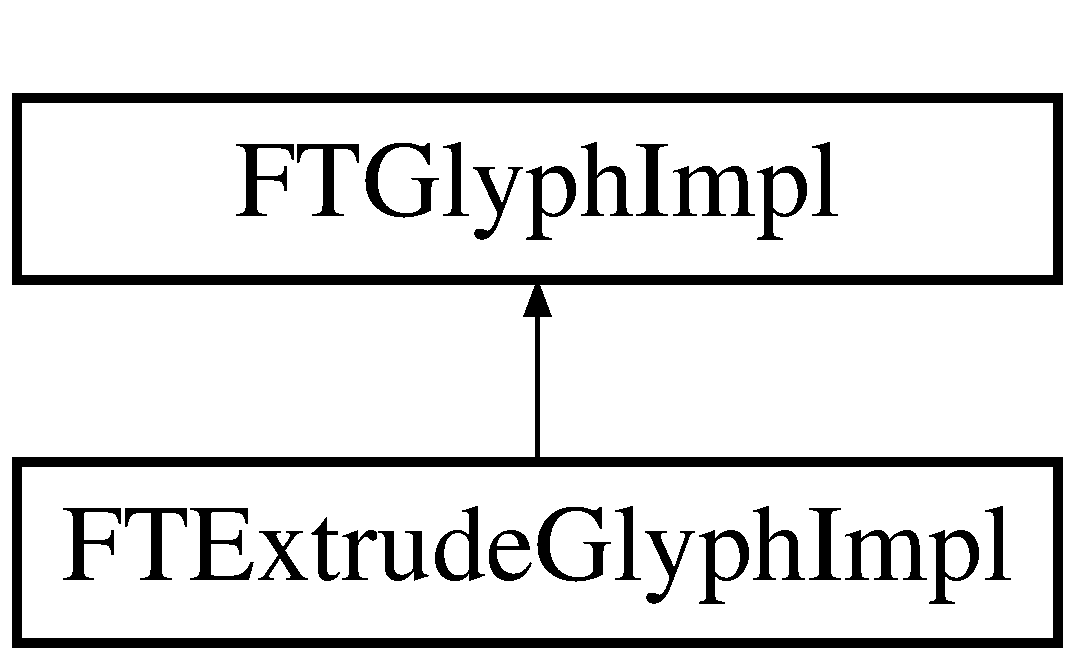
\includegraphics[height=2.000000cm]{class_f_t_extrude_glyph_impl}
\end{center}
\end{figure}
\subsection*{Protected Member Functions}
\begin{DoxyCompactItemize}
\item 
\hypertarget{class_f_t_extrude_glyph_impl_adbfa8d05122539318f6caa8b77a5c291}{
{\bfseries FTExtrudeGlyphImpl} (\hyperlink{struct_f_t___glyph_slot_rec__}{FT\_\-GlyphSlot} glyph, float depth, float frontOutset, float backOutset, bool useDisplayList)}
\label{class_f_t_extrude_glyph_impl_adbfa8d05122539318f6caa8b77a5c291}

\item 
\hypertarget{class_f_t_extrude_glyph_impl_a7ba3363d6764a14a6954f068f626029b}{
virtual const FTPoint \& {\bfseries RenderImpl} (const FTPoint \&pen, int renderMode)}
\label{class_f_t_extrude_glyph_impl_a7ba3363d6764a14a6954f068f626029b}

\end{DoxyCompactItemize}
\subsection*{Friends}
\begin{DoxyCompactItemize}
\item 
\hypertarget{class_f_t_extrude_glyph_impl_a43bdcab05c1db93d9474fee8176c1fb0}{
class {\bfseries FTExtrudeGlyph}}
\label{class_f_t_extrude_glyph_impl_a43bdcab05c1db93d9474fee8176c1fb0}

\end{DoxyCompactItemize}


The documentation for this class was generated from the following files:\begin{DoxyCompactItemize}
\item 
src/libs/FTGL/FTGlyph/FTExtrudeGlyphImpl.h\item 
src/libs/FTGL/FTGlyph/FTExtrudeGlyph.cpp\end{DoxyCompactItemize}

\hypertarget{class_f_t_face}{
\section{FTFace Class Reference}
\label{class_f_t_face}\index{FTFace@{FTFace}}
}


{\ttfamily \#include $<$FTFace.h$>$}

\subsection*{Public Member Functions}
\begin{DoxyCompactItemize}
\item 
\hyperlink{class_f_t_face_a26907a8a50a1316799054454523f13b4}{FTFace} (const char $\ast$fontFilePath, bool precomputeKerning=true)
\item 
\hyperlink{class_f_t_face_a0c39392976775b415743326d2e478d57}{FTFace} (const unsigned char $\ast$pBufferBytes, size\_\-t bufferSizeInBytes, bool precomputeKerning=true)
\item 
virtual \hyperlink{class_f_t_face_aa7087c9bcd6a8c212bfe5048743d7872}{$\sim$FTFace} ()
\item 
bool \hyperlink{class_f_t_face_ac8521d2dc370555fea58a842bc4e8a65}{Attach} (const char $\ast$fontFilePath)
\item 
bool \hyperlink{class_f_t_face_a0ceddf4a66cb56457949307b613d0992}{Attach} (const unsigned char $\ast$pBufferBytes, size\_\-t bufferSizeInBytes)
\item 
\hyperlink{struct_f_t___face_rec__}{FT\_\-Face} $\ast$ \hyperlink{class_f_t_face_ad3e6e4dcd0d84ad3e80f6c0a4e12f233}{Face} () const 
\item 
const \hyperlink{class_f_t_size}{FTSize} \& \hyperlink{class_f_t_face_a9fb537b25a678a783aa07da8acf1280b}{Size} (const unsigned int size, const unsigned int res)
\item 
unsigned int \hyperlink{class_f_t_face_ab1ee1e2906909c8d42e1c143d23b2f5d}{CharMapCount} () const 
\item 
FT\_\-Encoding $\ast$ \hyperlink{class_f_t_face_ae937a2a2c94f933bddb2619d96cad74e}{CharMapList} ()
\item 
FTPoint \hyperlink{class_f_t_face_af57bd3a3122e0e54acb04b348380ed7e}{KernAdvance} (unsigned int index1, unsigned int index2)
\item 
\hyperlink{struct_f_t___glyph_slot_rec__}{FT\_\-GlyphSlot} \hyperlink{class_f_t_face_aad153f57e7eb55ff42755b0512b01854}{Glyph} (unsigned int index, FT\_\-Int load\_\-flags)
\item 
unsigned int \hyperlink{class_f_t_face_a58805c5cf39daeb8d3fa11e2f791c31a}{GlyphCount} () const 
\item 
FT\_\-Error \hyperlink{class_f_t_face_a7caba7cdfdc277dc377aed97ab1b36b4}{Error} () const 
\end{DoxyCompactItemize}


\subsection{Detailed Description}
\hyperlink{class_f_t_face}{FTFace} class provides an abstraction layer for the Freetype Face.

\begin{DoxySeeAlso}{See also}
\char`\"{}Freetype 2 Documentation\char`\"{} 
\end{DoxySeeAlso}


\subsection{Constructor \& Destructor Documentation}
\hypertarget{class_f_t_face_a26907a8a50a1316799054454523f13b4}{
\index{FTFace@{FTFace}!FTFace@{FTFace}}
\index{FTFace@{FTFace}!FTFace@{FTFace}}
\subsubsection[{FTFace}]{\setlength{\rightskip}{0pt plus 5cm}FTFace::FTFace (
\begin{DoxyParamCaption}
\item[{const char $\ast$}]{ fontFilePath, }
\item[{bool}]{ precomputeKerning = {\ttfamily true}}
\end{DoxyParamCaption}
)}}
\label{class_f_t_face_a26907a8a50a1316799054454523f13b4}
Opens and reads a face file. Error is set.


\begin{DoxyParams}{Parameters}
{\em fontFilePath} & font file path. \\
\hline
\end{DoxyParams}
\hypertarget{class_f_t_face_a0c39392976775b415743326d2e478d57}{
\index{FTFace@{FTFace}!FTFace@{FTFace}}
\index{FTFace@{FTFace}!FTFace@{FTFace}}
\subsubsection[{FTFace}]{\setlength{\rightskip}{0pt plus 5cm}FTFace::FTFace (
\begin{DoxyParamCaption}
\item[{const unsigned char $\ast$}]{ pBufferBytes, }
\item[{size\_\-t}]{ bufferSizeInBytes, }
\item[{bool}]{ precomputeKerning = {\ttfamily true}}
\end{DoxyParamCaption}
)}}
\label{class_f_t_face_a0c39392976775b415743326d2e478d57}
Read face data from an in-\/memory buffer. Error is set.


\begin{DoxyParams}{Parameters}
{\em pBufferBytes} & the in-\/memory buffer \\
\hline
{\em bufferSizeInBytes} & the length of the buffer in bytes \\
\hline
\end{DoxyParams}
\hypertarget{class_f_t_face_aa7087c9bcd6a8c212bfe5048743d7872}{
\index{FTFace@{FTFace}!$\sim$FTFace@{$\sim$FTFace}}
\index{$\sim$FTFace@{$\sim$FTFace}!FTFace@{FTFace}}
\subsubsection[{$\sim$FTFace}]{\setlength{\rightskip}{0pt plus 5cm}FTFace::$\sim$FTFace (
\begin{DoxyParamCaption}
{}
\end{DoxyParamCaption}
)\hspace{0.3cm}{\ttfamily  \mbox{[}virtual\mbox{]}}}}
\label{class_f_t_face_aa7087c9bcd6a8c212bfe5048743d7872}
Destructor

Disposes of the current Freetype Face. 

\subsection{Member Function Documentation}
\hypertarget{class_f_t_face_ac8521d2dc370555fea58a842bc4e8a65}{
\index{FTFace@{FTFace}!Attach@{Attach}}
\index{Attach@{Attach}!FTFace@{FTFace}}
\subsubsection[{Attach}]{\setlength{\rightskip}{0pt plus 5cm}bool FTFace::Attach (
\begin{DoxyParamCaption}
\item[{const char $\ast$}]{ fontFilePath}
\end{DoxyParamCaption}
)}}
\label{class_f_t_face_ac8521d2dc370555fea58a842bc4e8a65}
Attach auxilliary file to font (e.g., font metrics).


\begin{DoxyParams}{Parameters}
{\em fontFilePath} & auxilliary font file path. \\
\hline
\end{DoxyParams}
\begin{DoxyReturn}{Returns}
{\ttfamily true} if file has opened successfully. 
\end{DoxyReturn}
\hypertarget{class_f_t_face_a0ceddf4a66cb56457949307b613d0992}{
\index{FTFace@{FTFace}!Attach@{Attach}}
\index{Attach@{Attach}!FTFace@{FTFace}}
\subsubsection[{Attach}]{\setlength{\rightskip}{0pt plus 5cm}bool FTFace::Attach (
\begin{DoxyParamCaption}
\item[{const unsigned char $\ast$}]{ pBufferBytes, }
\item[{size\_\-t}]{ bufferSizeInBytes}
\end{DoxyParamCaption}
)}}
\label{class_f_t_face_a0ceddf4a66cb56457949307b613d0992}
Attach auxilliary data to font (e.g., font metrics) from memory


\begin{DoxyParams}{Parameters}
{\em pBufferBytes} & the in-\/memory buffer \\
\hline
{\em bufferSizeInBytes} & the length of the buffer in bytes \\
\hline
\end{DoxyParams}
\begin{DoxyReturn}{Returns}
{\ttfamily true} if file has opened successfully. 
\end{DoxyReturn}
\hypertarget{class_f_t_face_ab1ee1e2906909c8d42e1c143d23b2f5d}{
\index{FTFace@{FTFace}!CharMapCount@{CharMapCount}}
\index{CharMapCount@{CharMapCount}!FTFace@{FTFace}}
\subsubsection[{CharMapCount}]{\setlength{\rightskip}{0pt plus 5cm}unsigned int FTFace::CharMapCount (
\begin{DoxyParamCaption}
{}
\end{DoxyParamCaption}
) const}}
\label{class_f_t_face_ab1ee1e2906909c8d42e1c143d23b2f5d}
Get the number of character maps in this face.

\begin{DoxyReturn}{Returns}
character map count. 
\end{DoxyReturn}
\hypertarget{class_f_t_face_ae937a2a2c94f933bddb2619d96cad74e}{
\index{FTFace@{FTFace}!CharMapList@{CharMapList}}
\index{CharMapList@{CharMapList}!FTFace@{FTFace}}
\subsubsection[{CharMapList}]{\setlength{\rightskip}{0pt plus 5cm}FT\_\-Encoding $\ast$ FTFace::CharMapList (
\begin{DoxyParamCaption}
{}
\end{DoxyParamCaption}
)}}
\label{class_f_t_face_ae937a2a2c94f933bddb2619d96cad74e}
Get a list of character maps in this face.

\begin{DoxyReturn}{Returns}
pointer to the first encoding. 
\end{DoxyReturn}
\hypertarget{class_f_t_face_a7caba7cdfdc277dc377aed97ab1b36b4}{
\index{FTFace@{FTFace}!Error@{Error}}
\index{Error@{Error}!FTFace@{FTFace}}
\subsubsection[{Error}]{\setlength{\rightskip}{0pt plus 5cm}FT\_\-Error FTFace::Error (
\begin{DoxyParamCaption}
{}
\end{DoxyParamCaption}
) const\hspace{0.3cm}{\ttfamily  \mbox{[}inline\mbox{]}}}}
\label{class_f_t_face_a7caba7cdfdc277dc377aed97ab1b36b4}
Queries for errors.

\begin{DoxyReturn}{Returns}
The current error code. 
\end{DoxyReturn}
\hypertarget{class_f_t_face_ad3e6e4dcd0d84ad3e80f6c0a4e12f233}{
\index{FTFace@{FTFace}!Face@{Face}}
\index{Face@{Face}!FTFace@{FTFace}}
\subsubsection[{Face}]{\setlength{\rightskip}{0pt plus 5cm}{\bf FT\_\-Face}$\ast$ FTFace::Face (
\begin{DoxyParamCaption}
{}
\end{DoxyParamCaption}
) const\hspace{0.3cm}{\ttfamily  \mbox{[}inline\mbox{]}}}}
\label{class_f_t_face_ad3e6e4dcd0d84ad3e80f6c0a4e12f233}
Get the freetype face object..

\begin{DoxyReturn}{Returns}
pointer to an FT\_\-Face. 
\end{DoxyReturn}
\hypertarget{class_f_t_face_aad153f57e7eb55ff42755b0512b01854}{
\index{FTFace@{FTFace}!Glyph@{Glyph}}
\index{Glyph@{Glyph}!FTFace@{FTFace}}
\subsubsection[{Glyph}]{\setlength{\rightskip}{0pt plus 5cm}{\bf FT\_\-GlyphSlot} FTFace::Glyph (
\begin{DoxyParamCaption}
\item[{unsigned int}]{ index, }
\item[{FT\_\-Int}]{ load\_\-flags}
\end{DoxyParamCaption}
)}}
\label{class_f_t_face_aad153f57e7eb55ff42755b0512b01854}
Loads and creates a Freetype glyph. \hypertarget{class_f_t_face_a58805c5cf39daeb8d3fa11e2f791c31a}{
\index{FTFace@{FTFace}!GlyphCount@{GlyphCount}}
\index{GlyphCount@{GlyphCount}!FTFace@{FTFace}}
\subsubsection[{GlyphCount}]{\setlength{\rightskip}{0pt plus 5cm}unsigned int FTFace::GlyphCount (
\begin{DoxyParamCaption}
{}
\end{DoxyParamCaption}
) const\hspace{0.3cm}{\ttfamily  \mbox{[}inline\mbox{]}}}}
\label{class_f_t_face_a58805c5cf39daeb8d3fa11e2f791c31a}
Gets the number of glyphs in the current face. \hypertarget{class_f_t_face_af57bd3a3122e0e54acb04b348380ed7e}{
\index{FTFace@{FTFace}!KernAdvance@{KernAdvance}}
\index{KernAdvance@{KernAdvance}!FTFace@{FTFace}}
\subsubsection[{KernAdvance}]{\setlength{\rightskip}{0pt plus 5cm}FTPoint FTFace::KernAdvance (
\begin{DoxyParamCaption}
\item[{unsigned int}]{ index1, }
\item[{unsigned int}]{ index2}
\end{DoxyParamCaption}
)}}
\label{class_f_t_face_af57bd3a3122e0e54acb04b348380ed7e}
Gets the kerning vector between two glyphs \hypertarget{class_f_t_face_a9fb537b25a678a783aa07da8acf1280b}{
\index{FTFace@{FTFace}!Size@{Size}}
\index{Size@{Size}!FTFace@{FTFace}}
\subsubsection[{Size}]{\setlength{\rightskip}{0pt plus 5cm}const {\bf FTSize} \& FTFace::Size (
\begin{DoxyParamCaption}
\item[{const unsigned int}]{ size, }
\item[{const unsigned int}]{ res}
\end{DoxyParamCaption}
)}}
\label{class_f_t_face_a9fb537b25a678a783aa07da8acf1280b}
Sets the char size for the current face.

This doesn't guarantee that the size was set correctly. Clients should check errors.


\begin{DoxyParams}{Parameters}
{\em size} & the face size in points (1/72 inch) \\
\hline
{\em res} & the resolution of the target device. \\
\hline
\end{DoxyParams}
\begin{DoxyReturn}{Returns}
{\ttfamily \hyperlink{class_f_t_size}{FTSize}} object 
\end{DoxyReturn}


The documentation for this class was generated from the following files:\begin{DoxyCompactItemize}
\item 
src/libs/FTGL/FTFace.h\item 
src/libs/FTGL/FTFace.cpp\end{DoxyCompactItemize}

\hypertarget{class_f_t_font_impl}{
\section{FTFontImpl Class Reference}
\label{class_f_t_font_impl}\index{FTFontImpl@{FTFontImpl}}
}
Inheritance diagram for FTFontImpl:\begin{figure}[H]
\begin{center}
\leavevmode
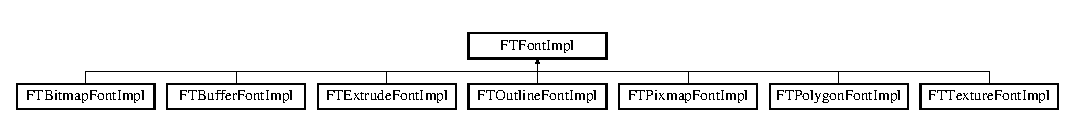
\includegraphics[height=1.250000cm]{class_f_t_font_impl}
\end{center}
\end{figure}
\subsection*{Protected Member Functions}
\begin{DoxyCompactItemize}
\item 
\hypertarget{class_f_t_font_impl_a4b0a3bd10221f8d51b4ca651c09a9cc5}{
{\bfseries FTFontImpl} (FTFont $\ast$ftFont, char const $\ast$fontFilePath)}
\label{class_f_t_font_impl_a4b0a3bd10221f8d51b4ca651c09a9cc5}

\item 
\hypertarget{class_f_t_font_impl_a1672e949c774c02a1642cdd090dddfc1}{
{\bfseries FTFontImpl} (FTFont $\ast$ftFont, const unsigned char $\ast$pBufferBytes, size\_\-t bufferSizeInBytes)}
\label{class_f_t_font_impl_a1672e949c774c02a1642cdd090dddfc1}

\item 
\hypertarget{class_f_t_font_impl_af96aac1ae6b457b52404bb268dd8b726}{
virtual bool {\bfseries Attach} (const char $\ast$fontFilePath)}
\label{class_f_t_font_impl_af96aac1ae6b457b52404bb268dd8b726}

\item 
\hypertarget{class_f_t_font_impl_af87c2267ecc8fa7eb717a8db9eb71ae6}{
virtual bool {\bfseries Attach} (const unsigned char $\ast$pBufferBytes, size\_\-t bufferSizeInBytes)}
\label{class_f_t_font_impl_af87c2267ecc8fa7eb717a8db9eb71ae6}

\item 
\hypertarget{class_f_t_font_impl_ab9c1065b08407289d0fe5774a1fc6e07}{
virtual void {\bfseries GlyphLoadFlags} (FT\_\-Int flags)}
\label{class_f_t_font_impl_ab9c1065b08407289d0fe5774a1fc6e07}

\item 
\hypertarget{class_f_t_font_impl_ac6ed6571c7b704610a0a78159663359d}{
virtual bool {\bfseries CharMap} (FT\_\-Encoding encoding)}
\label{class_f_t_font_impl_ac6ed6571c7b704610a0a78159663359d}

\item 
\hypertarget{class_f_t_font_impl_a54770e1ab6374469661d6b59684d2130}{
virtual unsigned int {\bfseries CharMapCount} () const }
\label{class_f_t_font_impl_a54770e1ab6374469661d6b59684d2130}

\item 
\hypertarget{class_f_t_font_impl_a5f632609c3368c12b9c19a05fd773bae}{
virtual FT\_\-Encoding $\ast$ {\bfseries CharMapList} ()}
\label{class_f_t_font_impl_a5f632609c3368c12b9c19a05fd773bae}

\item 
\hypertarget{class_f_t_font_impl_a8a83cfafb686a182b333d5002590a020}{
virtual void {\bfseries UseDisplayList} (bool useList)}
\label{class_f_t_font_impl_a8a83cfafb686a182b333d5002590a020}

\item 
\hypertarget{class_f_t_font_impl_a1f9b94b11bdb3b6181846572a5fe767f}{
virtual float {\bfseries Ascender} () const }
\label{class_f_t_font_impl_a1f9b94b11bdb3b6181846572a5fe767f}

\item 
\hypertarget{class_f_t_font_impl_a2a755f954a2a7aa5e69a9e9e6cf14ab1}{
virtual float {\bfseries Descender} () const }
\label{class_f_t_font_impl_a2a755f954a2a7aa5e69a9e9e6cf14ab1}

\item 
\hypertarget{class_f_t_font_impl_a00a4e10887f305f986737fc102e88a6b}{
virtual float {\bfseries LineHeight} () const }
\label{class_f_t_font_impl_a00a4e10887f305f986737fc102e88a6b}

\item 
\hypertarget{class_f_t_font_impl_a0739028e23c1c3d05f6db80b14428dde}{
virtual bool {\bfseries FaceSize} (const unsigned int size, const unsigned int res)}
\label{class_f_t_font_impl_a0739028e23c1c3d05f6db80b14428dde}

\item 
\hypertarget{class_f_t_font_impl_a099a32e288dd0e0d7674b29a170ab52c}{
virtual unsigned int {\bfseries FaceSize} () const }
\label{class_f_t_font_impl_a099a32e288dd0e0d7674b29a170ab52c}

\item 
\hypertarget{class_f_t_font_impl_a534a812f2df93e40392c9c5eca423b3f}{
virtual void {\bfseries Depth} (float depth)}
\label{class_f_t_font_impl_a534a812f2df93e40392c9c5eca423b3f}

\item 
\hypertarget{class_f_t_font_impl_aaa36154bf49c163d58d5b36575e23348}{
virtual void {\bfseries Outset} (float outset)}
\label{class_f_t_font_impl_aaa36154bf49c163d58d5b36575e23348}

\item 
\hypertarget{class_f_t_font_impl_a848e50bd8b6602ab7664e6d8c32167d3}{
virtual void {\bfseries Outset} (float front, float back)}
\label{class_f_t_font_impl_a848e50bd8b6602ab7664e6d8c32167d3}

\item 
\hypertarget{class_f_t_font_impl_ad26207fc1c4d70d1f800857f3893c8a1}{
virtual FTBBox {\bfseries BBox} (const char $\ast$s, const int len, FTPoint, FTPoint)}
\label{class_f_t_font_impl_ad26207fc1c4d70d1f800857f3893c8a1}

\item 
\hypertarget{class_f_t_font_impl_a13a17b5af83b6d81aea4a297646789e0}{
virtual FTBBox {\bfseries BBox} (const wchar\_\-t $\ast$s, const int len, FTPoint, FTPoint)}
\label{class_f_t_font_impl_a13a17b5af83b6d81aea4a297646789e0}

\item 
\hypertarget{class_f_t_font_impl_a237dc30760ac7d1b1e321da179a5055a}{
virtual float {\bfseries Advance} (const char $\ast$s, const int len, FTPoint)}
\label{class_f_t_font_impl_a237dc30760ac7d1b1e321da179a5055a}

\item 
\hypertarget{class_f_t_font_impl_a802bd5a2eefad0cdc27b22b63dab3de0}{
virtual float {\bfseries Advance} (const wchar\_\-t $\ast$s, const int len, FTPoint)}
\label{class_f_t_font_impl_a802bd5a2eefad0cdc27b22b63dab3de0}

\item 
\hypertarget{class_f_t_font_impl_a1562233a391c602c155ee6ce5df8b4e9}{
virtual FTPoint {\bfseries Render} (const char $\ast$s, const int len, FTPoint, FTPoint, int)}
\label{class_f_t_font_impl_a1562233a391c602c155ee6ce5df8b4e9}

\item 
\hypertarget{class_f_t_font_impl_ad6f899bf03a580f616c8238b5ea0f419}{
virtual FTPoint {\bfseries Render} (const wchar\_\-t $\ast$s, const int len, FTPoint, FTPoint, int)}
\label{class_f_t_font_impl_ad6f899bf03a580f616c8238b5ea0f419}

\end{DoxyCompactItemize}
\subsection*{Protected Attributes}
\begin{DoxyCompactItemize}
\item 
\hyperlink{class_f_t_face}{FTFace} \hyperlink{class_f_t_font_impl_ab35b9e1966574c6bb88bff520e9c33df}{face}
\item 
\hyperlink{class_f_t_size}{FTSize} \hyperlink{class_f_t_font_impl_a9ec32ea40b0d1ea53442daec1bbaade1}{charSize}
\item 
bool \hyperlink{class_f_t_font_impl_a5c21ea909477c7180b86625fef6af457}{useDisplayLists}
\item 
FT\_\-Int \hyperlink{class_f_t_font_impl_a217737b273e6abaa0dd6d837d5677e56}{load\_\-flags}
\item 
FT\_\-Error \hyperlink{class_f_t_font_impl_a39510c5a3665ae65bc7ff9b96c25b0c9}{err}
\end{DoxyCompactItemize}
\subsection*{Friends}
\begin{DoxyCompactItemize}
\item 
\hypertarget{class_f_t_font_impl_a8db85445a08f6c3139ba842b37e5b183}{
class {\bfseries FTFont}}
\label{class_f_t_font_impl_a8db85445a08f6c3139ba842b37e5b183}

\end{DoxyCompactItemize}


\subsection{Member Data Documentation}
\hypertarget{class_f_t_font_impl_a9ec32ea40b0d1ea53442daec1bbaade1}{
\index{FTFontImpl@{FTFontImpl}!charSize@{charSize}}
\index{charSize@{charSize}!FTFontImpl@{FTFontImpl}}
\subsubsection[{charSize}]{\setlength{\rightskip}{0pt plus 5cm}{\bf FTSize} {\bf FTFontImpl::charSize}\hspace{0.3cm}{\ttfamily  \mbox{[}protected\mbox{]}}}}
\label{class_f_t_font_impl_a9ec32ea40b0d1ea53442daec1bbaade1}
Current size object \hypertarget{class_f_t_font_impl_a39510c5a3665ae65bc7ff9b96c25b0c9}{
\index{FTFontImpl@{FTFontImpl}!err@{err}}
\index{err@{err}!FTFontImpl@{FTFontImpl}}
\subsubsection[{err}]{\setlength{\rightskip}{0pt plus 5cm}FT\_\-Error {\bf FTFontImpl::err}\hspace{0.3cm}{\ttfamily  \mbox{[}protected\mbox{]}}}}
\label{class_f_t_font_impl_a39510c5a3665ae65bc7ff9b96c25b0c9}
Current error code. Zero means no error. \hypertarget{class_f_t_font_impl_ab35b9e1966574c6bb88bff520e9c33df}{
\index{FTFontImpl@{FTFontImpl}!face@{face}}
\index{face@{face}!FTFontImpl@{FTFontImpl}}
\subsubsection[{face}]{\setlength{\rightskip}{0pt plus 5cm}{\bf FTFace} {\bf FTFontImpl::face}\hspace{0.3cm}{\ttfamily  \mbox{[}protected\mbox{]}}}}
\label{class_f_t_font_impl_ab35b9e1966574c6bb88bff520e9c33df}
Current face object \hypertarget{class_f_t_font_impl_a217737b273e6abaa0dd6d837d5677e56}{
\index{FTFontImpl@{FTFontImpl}!load\_\-flags@{load\_\-flags}}
\index{load\_\-flags@{load\_\-flags}!FTFontImpl@{FTFontImpl}}
\subsubsection[{load\_\-flags}]{\setlength{\rightskip}{0pt plus 5cm}FT\_\-Int {\bf FTFontImpl::load\_\-flags}\hspace{0.3cm}{\ttfamily  \mbox{[}protected\mbox{]}}}}
\label{class_f_t_font_impl_a217737b273e6abaa0dd6d837d5677e56}
The default glyph loading flags. \hypertarget{class_f_t_font_impl_a5c21ea909477c7180b86625fef6af457}{
\index{FTFontImpl@{FTFontImpl}!useDisplayLists@{useDisplayLists}}
\index{useDisplayLists@{useDisplayLists}!FTFontImpl@{FTFontImpl}}
\subsubsection[{useDisplayLists}]{\setlength{\rightskip}{0pt plus 5cm}bool {\bf FTFontImpl::useDisplayLists}\hspace{0.3cm}{\ttfamily  \mbox{[}protected\mbox{]}}}}
\label{class_f_t_font_impl_a5c21ea909477c7180b86625fef6af457}
Flag to enable or disable the use of Display Lists inside FTGL {\ttfamily true} turns ON display lists. {\ttfamily false} turns OFF display lists. 

The documentation for this class was generated from the following files:\begin{DoxyCompactItemize}
\item 
src/libs/FTGL/FTFont/FTFontImpl.h\item 
src/libs/FTGL/FTFont/FTFont.cpp\end{DoxyCompactItemize}

\hypertarget{class_f_t_glyph_container}{
\section{FTGlyphContainer Class Reference}
\label{class_f_t_glyph_container}\index{FTGlyphContainer@{FTGlyphContainer}}
}


{\ttfamily \#include $<$FTGlyphContainer.h$>$}

\subsection*{Public Member Functions}
\begin{DoxyCompactItemize}
\item 
\hyperlink{class_f_t_glyph_container_a277feb3b5aec44774f34957405f8bd33}{FTGlyphContainer} (\hyperlink{class_f_t_face}{FTFace} $\ast$face)
\item 
\hyperlink{class_f_t_glyph_container_a37389dc7c5764dbeb97d0e89ca92337a}{$\sim$FTGlyphContainer} ()
\item 
bool \hyperlink{class_f_t_glyph_container_af733b9a0df70930abc1091571287e820}{CharMap} (FT\_\-Encoding encoding)
\item 
unsigned int \hyperlink{class_f_t_glyph_container_a65f816bf2a49eb378a006c17e69455a7}{FontIndex} (const unsigned int characterCode) const 
\item 
void \hyperlink{class_f_t_glyph_container_ae8f085d829fce8d00479873058bc5ebe}{Add} (FTGlyph $\ast$glyph, const unsigned int characterCode)
\item 
const FTGlyph $\ast$const \hyperlink{class_f_t_glyph_container_a87feabeda7c963135f5618912f9dd483}{Glyph} (const unsigned int characterCode) const 
\item 
FTBBox \hyperlink{class_f_t_glyph_container_acb4b272ab8234d70091a3c79a373d4e0}{BBox} (const unsigned int characterCode) const 
\item 
float \hyperlink{class_f_t_glyph_container_ab57f99b48c5991558284bd85504291b1}{Advance} (const unsigned int characterCode, const unsigned int nextCharacterCode)
\item 
FTPoint \hyperlink{class_f_t_glyph_container_a4c3f9e0cd676f07a249a6dc18bea5d05}{Render} (const unsigned int characterCode, const unsigned int nextCharacterCode, FTPoint penPosition, int renderMode)
\item 
FT\_\-Error \hyperlink{class_f_t_glyph_container_a4b0b0368c93f3db09d6fcadaddde2a18}{Error} () const 
\end{DoxyCompactItemize}


\subsection{Detailed Description}
\hyperlink{class_f_t_glyph_container}{FTGlyphContainer} holds the post processed FTGlyph objects.

\begin{DoxySeeAlso}{See also}
FTGlyph 
\end{DoxySeeAlso}


\subsection{Constructor \& Destructor Documentation}
\hypertarget{class_f_t_glyph_container_a277feb3b5aec44774f34957405f8bd33}{
\index{FTGlyphContainer@{FTGlyphContainer}!FTGlyphContainer@{FTGlyphContainer}}
\index{FTGlyphContainer@{FTGlyphContainer}!FTGlyphContainer@{FTGlyphContainer}}
\subsubsection[{FTGlyphContainer}]{\setlength{\rightskip}{0pt plus 5cm}FTGlyphContainer::FTGlyphContainer (
\begin{DoxyParamCaption}
\item[{{\bf FTFace} $\ast$}]{ face}
\end{DoxyParamCaption}
)}}
\label{class_f_t_glyph_container_a277feb3b5aec44774f34957405f8bd33}
Constructor


\begin{DoxyParams}{Parameters}
{\em face} & The Freetype face \\
\hline
\end{DoxyParams}
\hypertarget{class_f_t_glyph_container_a37389dc7c5764dbeb97d0e89ca92337a}{
\index{FTGlyphContainer@{FTGlyphContainer}!$\sim$FTGlyphContainer@{$\sim$FTGlyphContainer}}
\index{$\sim$FTGlyphContainer@{$\sim$FTGlyphContainer}!FTGlyphContainer@{FTGlyphContainer}}
\subsubsection[{$\sim$FTGlyphContainer}]{\setlength{\rightskip}{0pt plus 5cm}FTGlyphContainer::$\sim$FTGlyphContainer (
\begin{DoxyParamCaption}
{}
\end{DoxyParamCaption}
)}}
\label{class_f_t_glyph_container_a37389dc7c5764dbeb97d0e89ca92337a}
Destructor 

\subsection{Member Function Documentation}
\hypertarget{class_f_t_glyph_container_ae8f085d829fce8d00479873058bc5ebe}{
\index{FTGlyphContainer@{FTGlyphContainer}!Add@{Add}}
\index{Add@{Add}!FTGlyphContainer@{FTGlyphContainer}}
\subsubsection[{Add}]{\setlength{\rightskip}{0pt plus 5cm}void FTGlyphContainer::Add (
\begin{DoxyParamCaption}
\item[{FTGlyph $\ast$}]{ glyph, }
\item[{const unsigned int}]{ characterCode}
\end{DoxyParamCaption}
)}}
\label{class_f_t_glyph_container_ae8f085d829fce8d00479873058bc5ebe}
Adds a glyph to this glyph list.


\begin{DoxyParams}{Parameters}
{\em glyph} & The FTGlyph to be inserted into the container \\
\hline
{\em characterCode} & The char code of the glyph NOT the glyph index. \\
\hline
\end{DoxyParams}
\hypertarget{class_f_t_glyph_container_ab57f99b48c5991558284bd85504291b1}{
\index{FTGlyphContainer@{FTGlyphContainer}!Advance@{Advance}}
\index{Advance@{Advance}!FTGlyphContainer@{FTGlyphContainer}}
\subsubsection[{Advance}]{\setlength{\rightskip}{0pt plus 5cm}float FTGlyphContainer::Advance (
\begin{DoxyParamCaption}
\item[{const unsigned int}]{ characterCode, }
\item[{const unsigned int}]{ nextCharacterCode}
\end{DoxyParamCaption}
)}}
\label{class_f_t_glyph_container_ab57f99b48c5991558284bd85504291b1}
Returns the kerned advance width for a glyph.


\begin{DoxyParams}{Parameters}
{\em characterCode} & glyph index of the character \\
\hline
{\em nextCharacterCode} & the next glyph in a string \\
\hline
\end{DoxyParams}
\begin{DoxyReturn}{Returns}
advance width 
\end{DoxyReturn}
\hypertarget{class_f_t_glyph_container_acb4b272ab8234d70091a3c79a373d4e0}{
\index{FTGlyphContainer@{FTGlyphContainer}!BBox@{BBox}}
\index{BBox@{BBox}!FTGlyphContainer@{FTGlyphContainer}}
\subsubsection[{BBox}]{\setlength{\rightskip}{0pt plus 5cm}FTBBox FTGlyphContainer::BBox (
\begin{DoxyParamCaption}
\item[{const unsigned int}]{ characterCode}
\end{DoxyParamCaption}
) const}}
\label{class_f_t_glyph_container_acb4b272ab8234d70091a3c79a373d4e0}
Get the bounding box for a character. 
\begin{DoxyParams}{Parameters}
{\em characterCode} & The char code of the glyph NOT the glyph index \\
\hline
\end{DoxyParams}
\hypertarget{class_f_t_glyph_container_af733b9a0df70930abc1091571287e820}{
\index{FTGlyphContainer@{FTGlyphContainer}!CharMap@{CharMap}}
\index{CharMap@{CharMap}!FTGlyphContainer@{FTGlyphContainer}}
\subsubsection[{CharMap}]{\setlength{\rightskip}{0pt plus 5cm}bool FTGlyphContainer::CharMap (
\begin{DoxyParamCaption}
\item[{FT\_\-Encoding}]{ encoding}
\end{DoxyParamCaption}
)}}
\label{class_f_t_glyph_container_af733b9a0df70930abc1091571287e820}
Sets the character map for the face.


\begin{DoxyParams}{Parameters}
{\em encoding} & the Freetype encoding symbol. See above. \\
\hline
\end{DoxyParams}
\begin{DoxyReturn}{Returns}
{\ttfamily true} if charmap was valid and set correctly 
\end{DoxyReturn}
\hypertarget{class_f_t_glyph_container_a4b0b0368c93f3db09d6fcadaddde2a18}{
\index{FTGlyphContainer@{FTGlyphContainer}!Error@{Error}}
\index{Error@{Error}!FTGlyphContainer@{FTGlyphContainer}}
\subsubsection[{Error}]{\setlength{\rightskip}{0pt plus 5cm}FT\_\-Error FTGlyphContainer::Error (
\begin{DoxyParamCaption}
{}
\end{DoxyParamCaption}
) const\hspace{0.3cm}{\ttfamily  \mbox{[}inline\mbox{]}}}}
\label{class_f_t_glyph_container_a4b0b0368c93f3db09d6fcadaddde2a18}
Queries the \hyperlink{class_font}{Font} for errors.

\begin{DoxyReturn}{Returns}
The current error code. 
\end{DoxyReturn}
\hypertarget{class_f_t_glyph_container_a65f816bf2a49eb378a006c17e69455a7}{
\index{FTGlyphContainer@{FTGlyphContainer}!FontIndex@{FontIndex}}
\index{FontIndex@{FontIndex}!FTGlyphContainer@{FTGlyphContainer}}
\subsubsection[{FontIndex}]{\setlength{\rightskip}{0pt plus 5cm}unsigned int FTGlyphContainer::FontIndex (
\begin{DoxyParamCaption}
\item[{const unsigned int}]{ characterCode}
\end{DoxyParamCaption}
) const}}
\label{class_f_t_glyph_container_a65f816bf2a49eb378a006c17e69455a7}
Get the font index of the input character.


\begin{DoxyParams}{Parameters}
{\em characterCode} & The character code of the requested glyph in the current encoding eg apple roman. \\
\hline
\end{DoxyParams}
\begin{DoxyReturn}{Returns}
The font index for the character. 
\end{DoxyReturn}
\hypertarget{class_f_t_glyph_container_a87feabeda7c963135f5618912f9dd483}{
\index{FTGlyphContainer@{FTGlyphContainer}!Glyph@{Glyph}}
\index{Glyph@{Glyph}!FTGlyphContainer@{FTGlyphContainer}}
\subsubsection[{Glyph}]{\setlength{\rightskip}{0pt plus 5cm}const FTGlyph $\ast$const FTGlyphContainer::Glyph (
\begin{DoxyParamCaption}
\item[{const unsigned int}]{ characterCode}
\end{DoxyParamCaption}
) const}}
\label{class_f_t_glyph_container_a87feabeda7c963135f5618912f9dd483}
Get a glyph from the glyph list


\begin{DoxyParams}{Parameters}
{\em characterCode} & The char code of the glyph NOT the glyph index \\
\hline
\end{DoxyParams}
\begin{DoxyReturn}{Returns}
An FTGlyph or {\ttfamily null} is it hasn't been loaded. 
\end{DoxyReturn}
\hypertarget{class_f_t_glyph_container_a4c3f9e0cd676f07a249a6dc18bea5d05}{
\index{FTGlyphContainer@{FTGlyphContainer}!Render@{Render}}
\index{Render@{Render}!FTGlyphContainer@{FTGlyphContainer}}
\subsubsection[{Render}]{\setlength{\rightskip}{0pt plus 5cm}FTPoint FTGlyphContainer::Render (
\begin{DoxyParamCaption}
\item[{const unsigned int}]{ characterCode, }
\item[{const unsigned int}]{ nextCharacterCode, }
\item[{FTPoint}]{ penPosition, }
\item[{int}]{ renderMode}
\end{DoxyParamCaption}
)}}
\label{class_f_t_glyph_container_a4c3f9e0cd676f07a249a6dc18bea5d05}
Renders a character 
\begin{DoxyParams}{Parameters}
{\em characterCode} & the glyph to be Rendered \\
\hline
{\em nextCharacterCode} & the next glyph in the string. Used for kerning. \\
\hline
{\em penPosition} & the position to Render the glyph \\
\hline
{\em renderMode} & Render mode to display \\
\hline
\end{DoxyParams}
\begin{DoxyReturn}{Returns}
The distance to advance the pen position after Rendering 
\end{DoxyReturn}


The documentation for this class was generated from the following files:\begin{DoxyCompactItemize}
\item 
src/libs/FTGL/FTGlyphContainer.h\item 
src/libs/FTGL/FTGlyphContainer.cpp\end{DoxyCompactItemize}

\hypertarget{class_f_t_glyph_impl}{
\section{FTGlyphImpl Class Reference}
\label{class_f_t_glyph_impl}\index{FTGlyphImpl@{FTGlyphImpl}}
}
Inheritance diagram for FTGlyphImpl:\begin{figure}[H]
\begin{center}
\leavevmode
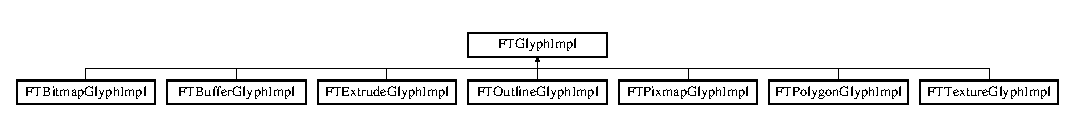
\includegraphics[height=1.176471cm]{class_f_t_glyph_impl}
\end{center}
\end{figure}
\subsection*{Protected Member Functions}
\begin{DoxyCompactItemize}
\item 
\hypertarget{class_f_t_glyph_impl_a1b4b16617fffb78e5abd3d293878872f}{
{\bfseries FTGlyphImpl} (\hyperlink{struct_f_t___glyph_slot_rec__}{FT\_\-GlyphSlot} glyph, bool useDisplayList=true)}
\label{class_f_t_glyph_impl_a1b4b16617fffb78e5abd3d293878872f}

\item 
\hypertarget{class_f_t_glyph_impl_a8e71d5a8e8137869ef629df6c5ba10a7}{
float {\bfseries Advance} () const }
\label{class_f_t_glyph_impl_a8e71d5a8e8137869ef629df6c5ba10a7}

\item 
\hypertarget{class_f_t_glyph_impl_a9780f42c30108d39be5b190cbc74d542}{
const FTBBox \& {\bfseries BBox} () const }
\label{class_f_t_glyph_impl_a9780f42c30108d39be5b190cbc74d542}

\item 
\hypertarget{class_f_t_glyph_impl_aca054d9ec6f56a6d96757c10ac4720f2}{
FT\_\-Error {\bfseries Error} () const }
\label{class_f_t_glyph_impl_aca054d9ec6f56a6d96757c10ac4720f2}

\end{DoxyCompactItemize}
\subsection*{Protected Attributes}
\begin{DoxyCompactItemize}
\item 
FTPoint \hyperlink{class_f_t_glyph_impl_acd0a260e13ec1714c2556d24a5352a31}{advance}
\item 
FTBBox \hyperlink{class_f_t_glyph_impl_a871a6a1a24be465bfae17b7a8e464b3c}{bBox}
\item 
FT\_\-Error \hyperlink{class_f_t_glyph_impl_a7a489998b09aef9ceb733604166e933c}{err}
\end{DoxyCompactItemize}
\subsection*{Friends}
\begin{DoxyCompactItemize}
\item 
\hypertarget{class_f_t_glyph_impl_a908ad68576153727d761f276dd8fd0e2}{
class {\bfseries FTGlyph}}
\label{class_f_t_glyph_impl_a908ad68576153727d761f276dd8fd0e2}

\end{DoxyCompactItemize}


\subsection{Member Data Documentation}
\hypertarget{class_f_t_glyph_impl_acd0a260e13ec1714c2556d24a5352a31}{
\index{FTGlyphImpl@{FTGlyphImpl}!advance@{advance}}
\index{advance@{advance}!FTGlyphImpl@{FTGlyphImpl}}
\subsubsection[{advance}]{\setlength{\rightskip}{0pt plus 5cm}FTPoint {\bf FTGlyphImpl::advance}\hspace{0.3cm}{\ttfamily  \mbox{[}protected\mbox{]}}}}
\label{class_f_t_glyph_impl_acd0a260e13ec1714c2556d24a5352a31}
The advance distance for this glyph \hypertarget{class_f_t_glyph_impl_a871a6a1a24be465bfae17b7a8e464b3c}{
\index{FTGlyphImpl@{FTGlyphImpl}!bBox@{bBox}}
\index{bBox@{bBox}!FTGlyphImpl@{FTGlyphImpl}}
\subsubsection[{bBox}]{\setlength{\rightskip}{0pt plus 5cm}FTBBox {\bf FTGlyphImpl::bBox}\hspace{0.3cm}{\ttfamily  \mbox{[}protected\mbox{]}}}}
\label{class_f_t_glyph_impl_a871a6a1a24be465bfae17b7a8e464b3c}
The bounding box of this glyph. \hypertarget{class_f_t_glyph_impl_a7a489998b09aef9ceb733604166e933c}{
\index{FTGlyphImpl@{FTGlyphImpl}!err@{err}}
\index{err@{err}!FTGlyphImpl@{FTGlyphImpl}}
\subsubsection[{err}]{\setlength{\rightskip}{0pt plus 5cm}FT\_\-Error {\bf FTGlyphImpl::err}\hspace{0.3cm}{\ttfamily  \mbox{[}protected\mbox{]}}}}
\label{class_f_t_glyph_impl_a7a489998b09aef9ceb733604166e933c}
Current error code. Zero means no error. 

The documentation for this class was generated from the following files:\begin{DoxyCompactItemize}
\item 
src/libs/FTGL/FTGlyph/FTGlyphImpl.h\item 
src/libs/FTGL/FTGlyph/FTGlyph.cpp\end{DoxyCompactItemize}

\hypertarget{class_f_t_layout_impl}{
\section{FTLayoutImpl Class Reference}
\label{class_f_t_layout_impl}\index{FTLayoutImpl@{FTLayoutImpl}}
}
Inheritance diagram for FTLayoutImpl:\begin{figure}[H]
\begin{center}
\leavevmode
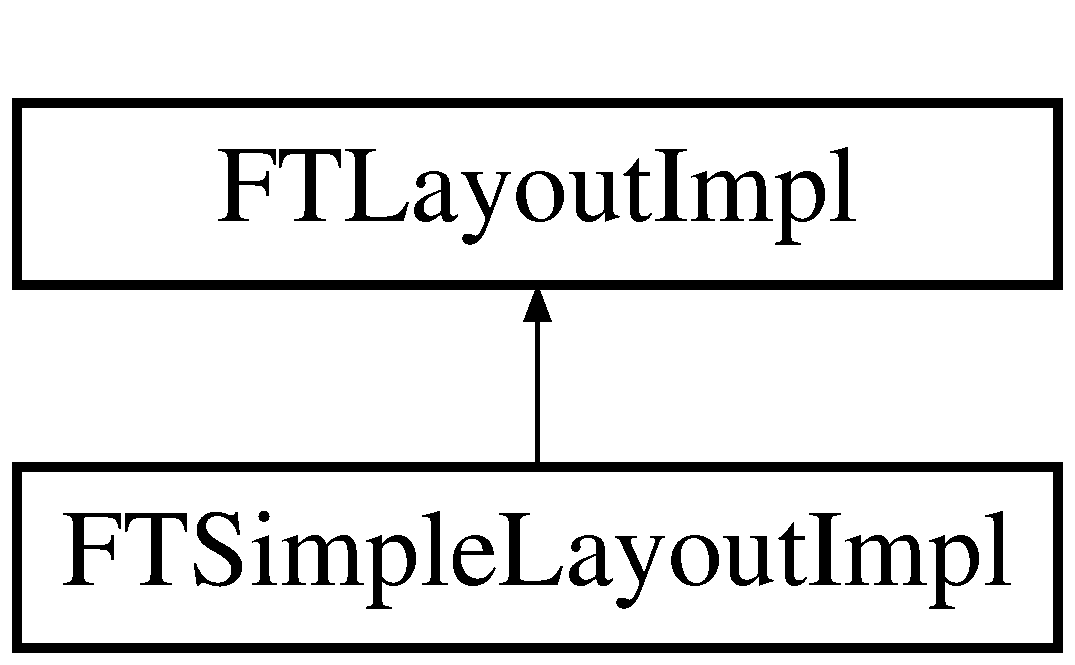
\includegraphics[height=2.000000cm]{class_f_t_layout_impl}
\end{center}
\end{figure}
\subsection*{Protected Attributes}
\begin{DoxyCompactItemize}
\item 
FTPoint \hyperlink{class_f_t_layout_impl_aefaff875c0cf4fe5710897f614be44ac}{pen}
\item 
FT\_\-Error \hyperlink{class_f_t_layout_impl_af3c9ad6d6636a69a6643d68383e4edcd}{err}
\end{DoxyCompactItemize}
\subsection*{Friends}
\begin{DoxyCompactItemize}
\item 
\hypertarget{class_f_t_layout_impl_a28e6cd087379e90923b29b9c2c103aa8}{
class {\bfseries FTLayout}}
\label{class_f_t_layout_impl_a28e6cd087379e90923b29b9c2c103aa8}

\end{DoxyCompactItemize}


\subsection{Member Data Documentation}
\hypertarget{class_f_t_layout_impl_af3c9ad6d6636a69a6643d68383e4edcd}{
\index{FTLayoutImpl@{FTLayoutImpl}!err@{err}}
\index{err@{err}!FTLayoutImpl@{FTLayoutImpl}}
\subsubsection[{err}]{\setlength{\rightskip}{0pt plus 5cm}FT\_\-Error {\bf FTLayoutImpl::err}\hspace{0.3cm}{\ttfamily  \mbox{[}protected\mbox{]}}}}
\label{class_f_t_layout_impl_af3c9ad6d6636a69a6643d68383e4edcd}
Current error code. Zero means no error. \hypertarget{class_f_t_layout_impl_aefaff875c0cf4fe5710897f614be44ac}{
\index{FTLayoutImpl@{FTLayoutImpl}!pen@{pen}}
\index{pen@{pen}!FTLayoutImpl@{FTLayoutImpl}}
\subsubsection[{pen}]{\setlength{\rightskip}{0pt plus 5cm}FTPoint {\bf FTLayoutImpl::pen}\hspace{0.3cm}{\ttfamily  \mbox{[}protected\mbox{]}}}}
\label{class_f_t_layout_impl_aefaff875c0cf4fe5710897f614be44ac}
Current pen or cursor position; 

The documentation for this class was generated from the following files:\begin{DoxyCompactItemize}
\item 
src/libs/FTGL/FTLayout/FTLayoutImpl.h\item 
src/libs/FTGL/FTLayout/FTLayout.cpp\end{DoxyCompactItemize}

\hypertarget{class_f_t_library}{
\section{FTLibrary Class Reference}
\label{class_f_t_library}\index{FTLibrary@{FTLibrary}}
}


{\ttfamily \#include $<$FTLibrary.h$>$}

\subsection*{Public Member Functions}
\begin{DoxyCompactItemize}
\item 
const \hyperlink{struct_f_t___library_rec__}{FT\_\-Library} $\ast$const \hyperlink{class_f_t_library_afef4db019eae5a4307201b7abc6a88c7}{GetLibrary} () const 
\item 
FT\_\-Error \hyperlink{class_f_t_library_ad01e538ba8e308dddda5c4ec808ee404}{Error} () const 
\item 
\hyperlink{class_f_t_library_a8d1ee3dc3c4916b5b428e934dc46e9d7}{$\sim$FTLibrary} ()
\end{DoxyCompactItemize}
\subsection*{Static Public Member Functions}
\begin{DoxyCompactItemize}
\item 
static const \hyperlink{class_f_t_library}{FTLibrary} \& \hyperlink{class_f_t_library_aa172665a8db8888851895bcb15aa8103}{Instance} ()
\end{DoxyCompactItemize}


\subsection{Detailed Description}
\hyperlink{class_f_t_library}{FTLibrary} class is the global accessor for the Freetype library.

This class encapsulates the Freetype Library. This is a singleton class and ensures that only one FT\_\-Library is in existence at any one time. All constructors are private therefore clients cannot create or instantiate this class themselves and must access it's methods via the static {\ttfamily \hyperlink{class_f_t_library_aa172665a8db8888851895bcb15aa8103}{FTLibrary::Instance()}} function.

Just because this class returns a valid {\ttfamily \hyperlink{class_f_t_library}{FTLibrary}} object doesn't mean that the Freetype Library has been successfully initialised. Clients should check for errors. You can initialse the library AND check for errors using the following code... {\ttfamily err = \hyperlink{class_f_t_library_aa172665a8db8888851895bcb15aa8103}{FTLibrary::Instance()}.\hyperlink{class_f_t_library_ad01e538ba8e308dddda5c4ec808ee404}{Error()};}

\begin{DoxySeeAlso}{See also}
\char`\"{}Freetype 2 Documentation\char`\"{} 
\end{DoxySeeAlso}


\subsection{Constructor \& Destructor Documentation}
\hypertarget{class_f_t_library_a8d1ee3dc3c4916b5b428e934dc46e9d7}{
\index{FTLibrary@{FTLibrary}!$\sim$FTLibrary@{$\sim$FTLibrary}}
\index{$\sim$FTLibrary@{$\sim$FTLibrary}!FTLibrary@{FTLibrary}}
\subsubsection[{$\sim$FTLibrary}]{\setlength{\rightskip}{0pt plus 5cm}FTLibrary::$\sim$FTLibrary (
\begin{DoxyParamCaption}
{}
\end{DoxyParamCaption}
)}}
\label{class_f_t_library_a8d1ee3dc3c4916b5b428e934dc46e9d7}
Destructor

Disposes of the Freetype library 

\subsection{Member Function Documentation}
\hypertarget{class_f_t_library_ad01e538ba8e308dddda5c4ec808ee404}{
\index{FTLibrary@{FTLibrary}!Error@{Error}}
\index{Error@{Error}!FTLibrary@{FTLibrary}}
\subsubsection[{Error}]{\setlength{\rightskip}{0pt plus 5cm}FT\_\-Error FTLibrary::Error (
\begin{DoxyParamCaption}
{}
\end{DoxyParamCaption}
) const\hspace{0.3cm}{\ttfamily  \mbox{[}inline\mbox{]}}}}
\label{class_f_t_library_ad01e538ba8e308dddda5c4ec808ee404}
Queries the library for errors.

\begin{DoxyReturn}{Returns}
The current error code. 
\end{DoxyReturn}
\hypertarget{class_f_t_library_afef4db019eae5a4307201b7abc6a88c7}{
\index{FTLibrary@{FTLibrary}!GetLibrary@{GetLibrary}}
\index{GetLibrary@{GetLibrary}!FTLibrary@{FTLibrary}}
\subsubsection[{GetLibrary}]{\setlength{\rightskip}{0pt plus 5cm}const {\bf FT\_\-Library}$\ast$ const FTLibrary::GetLibrary (
\begin{DoxyParamCaption}
{}
\end{DoxyParamCaption}
) const\hspace{0.3cm}{\ttfamily  \mbox{[}inline\mbox{]}}}}
\label{class_f_t_library_afef4db019eae5a4307201b7abc6a88c7}
Gets a pointer to the native Freetype library.

\begin{DoxyReturn}{Returns}
A handle to a FreeType library instance. 
\end{DoxyReturn}
\hypertarget{class_f_t_library_aa172665a8db8888851895bcb15aa8103}{
\index{FTLibrary@{FTLibrary}!Instance@{Instance}}
\index{Instance@{Instance}!FTLibrary@{FTLibrary}}
\subsubsection[{Instance}]{\setlength{\rightskip}{0pt plus 5cm}const {\bf FTLibrary} \& FTLibrary::Instance (
\begin{DoxyParamCaption}
{}
\end{DoxyParamCaption}
)\hspace{0.3cm}{\ttfamily  \mbox{[}static\mbox{]}}}}
\label{class_f_t_library_aa172665a8db8888851895bcb15aa8103}
Global acces point to the single \hyperlink{class_f_t_library}{FTLibrary} object.

\begin{DoxyReturn}{Returns}
The global {\ttfamily \hyperlink{class_f_t_library}{FTLibrary}} object. 
\end{DoxyReturn}


The documentation for this class was generated from the following files:\begin{DoxyCompactItemize}
\item 
src/libs/FTGL/FTLibrary.h\item 
src/libs/FTGL/FTLibrary.cpp\end{DoxyCompactItemize}

\hypertarget{class_f_t_list}{
\section{FTList$<$ FT\_\-LIST\_\-ITEM\_\-TYPE $>$ Class Template Reference}
\label{class_f_t_list}\index{FTList@{FTList}}
}


{\ttfamily \#include $<$FTList.h$>$}

\subsection*{Classes}
\begin{DoxyCompactItemize}
\item 
struct {\bfseries Node}
\end{DoxyCompactItemize}
\subsection*{Public Types}
\begin{DoxyCompactItemize}
\item 
\hypertarget{class_f_t_list_ae172da3e03bcd6dab4b5f60efe0fc7a3}{
typedef FT\_\-LIST\_\-ITEM\_\-TYPE {\bfseries value\_\-type}}
\label{class_f_t_list_ae172da3e03bcd6dab4b5f60efe0fc7a3}

\item 
\hypertarget{class_f_t_list_a37fe33040a67a2d5aad9ead2bb2179d7}{
typedef value\_\-type \& {\bfseries reference}}
\label{class_f_t_list_a37fe33040a67a2d5aad9ead2bb2179d7}

\item 
\hypertarget{class_f_t_list_a82677d676935b1f3cb5e9328523bf3a6}{
typedef const value\_\-type \& {\bfseries const\_\-reference}}
\label{class_f_t_list_a82677d676935b1f3cb5e9328523bf3a6}

\item 
\hypertarget{class_f_t_list_a5ebe9866c4f86791c6970f19deb09cb1}{
typedef size\_\-t {\bfseries size\_\-type}}
\label{class_f_t_list_a5ebe9866c4f86791c6970f19deb09cb1}

\end{DoxyCompactItemize}
\subsection*{Public Member Functions}
\begin{DoxyCompactItemize}
\item 
\hyperlink{class_f_t_list_a4de727811240b9d8568d1d47fd389502}{FTList} ()
\item 
\hyperlink{class_f_t_list_aabfac3b136119f727611d490aef3eab4}{$\sim$FTList} ()
\item 
size\_\-type \hyperlink{class_f_t_list_a73542705ba9556d5cd594c3ec32fe5d2}{size} () const 
\item 
void \hyperlink{class_f_t_list_acd30af5d1a32185842decac3e0c183ce}{push\_\-back} (const value\_\-type \&item)
\item 
reference \hyperlink{class_f_t_list_a068805ebb222e9ce69a8828b31fd87df}{front} () const 
\item 
reference \hyperlink{class_f_t_list_ae6b5f56991e9d2ac226ce7960e4661f4}{back} () const 
\end{DoxyCompactItemize}


\subsection{Detailed Description}
\subsubsection*{template$<$typename FT\_\-LIST\_\-ITEM\_\-TYPE$>$ class FTList$<$ FT\_\-LIST\_\-ITEM\_\-TYPE $>$}

Provides a non-\/STL alternative to the STL list 

\subsection{Constructor \& Destructor Documentation}
\hypertarget{class_f_t_list_a4de727811240b9d8568d1d47fd389502}{
\index{FTList@{FTList}!FTList@{FTList}}
\index{FTList@{FTList}!FTList@{FTList}}
\subsubsection[{FTList}]{\setlength{\rightskip}{0pt plus 5cm}template$<$typename FT\_\-LIST\_\-ITEM\_\-TYPE$>$ {\bf FTList}$<$ FT\_\-LIST\_\-ITEM\_\-TYPE $>$::{\bf FTList} (
\begin{DoxyParamCaption}
{}
\end{DoxyParamCaption}
)\hspace{0.3cm}{\ttfamily  \mbox{[}inline\mbox{]}}}}
\label{class_f_t_list_a4de727811240b9d8568d1d47fd389502}
Constructor \hypertarget{class_f_t_list_aabfac3b136119f727611d490aef3eab4}{
\index{FTList@{FTList}!$\sim$FTList@{$\sim$FTList}}
\index{$\sim$FTList@{$\sim$FTList}!FTList@{FTList}}
\subsubsection[{$\sim$FTList}]{\setlength{\rightskip}{0pt plus 5cm}template$<$typename FT\_\-LIST\_\-ITEM\_\-TYPE$>$ {\bf FTList}$<$ FT\_\-LIST\_\-ITEM\_\-TYPE $>$::$\sim${\bf FTList} (
\begin{DoxyParamCaption}
{}
\end{DoxyParamCaption}
)\hspace{0.3cm}{\ttfamily  \mbox{[}inline\mbox{]}}}}
\label{class_f_t_list_aabfac3b136119f727611d490aef3eab4}
Destructor 

\subsection{Member Function Documentation}
\hypertarget{class_f_t_list_ae6b5f56991e9d2ac226ce7960e4661f4}{
\index{FTList@{FTList}!back@{back}}
\index{back@{back}!FTList@{FTList}}
\subsubsection[{back}]{\setlength{\rightskip}{0pt plus 5cm}template$<$typename FT\_\-LIST\_\-ITEM\_\-TYPE$>$ reference {\bf FTList}$<$ FT\_\-LIST\_\-ITEM\_\-TYPE $>$::back (
\begin{DoxyParamCaption}
{}
\end{DoxyParamCaption}
) const\hspace{0.3cm}{\ttfamily  \mbox{[}inline\mbox{]}}}}
\label{class_f_t_list_ae6b5f56991e9d2ac226ce7960e4661f4}
Get the item at the end of the list \hypertarget{class_f_t_list_a068805ebb222e9ce69a8828b31fd87df}{
\index{FTList@{FTList}!front@{front}}
\index{front@{front}!FTList@{FTList}}
\subsubsection[{front}]{\setlength{\rightskip}{0pt plus 5cm}template$<$typename FT\_\-LIST\_\-ITEM\_\-TYPE$>$ reference {\bf FTList}$<$ FT\_\-LIST\_\-ITEM\_\-TYPE $>$::front (
\begin{DoxyParamCaption}
{}
\end{DoxyParamCaption}
) const\hspace{0.3cm}{\ttfamily  \mbox{[}inline\mbox{]}}}}
\label{class_f_t_list_a068805ebb222e9ce69a8828b31fd87df}
Get the item at the front of the list \hypertarget{class_f_t_list_acd30af5d1a32185842decac3e0c183ce}{
\index{FTList@{FTList}!push\_\-back@{push\_\-back}}
\index{push\_\-back@{push\_\-back}!FTList@{FTList}}
\subsubsection[{push\_\-back}]{\setlength{\rightskip}{0pt plus 5cm}template$<$typename FT\_\-LIST\_\-ITEM\_\-TYPE$>$ void {\bf FTList}$<$ FT\_\-LIST\_\-ITEM\_\-TYPE $>$::push\_\-back (
\begin{DoxyParamCaption}
\item[{const value\_\-type \&}]{ item}
\end{DoxyParamCaption}
)\hspace{0.3cm}{\ttfamily  \mbox{[}inline\mbox{]}}}}
\label{class_f_t_list_acd30af5d1a32185842decac3e0c183ce}
Add an item to the end of the list \hypertarget{class_f_t_list_a73542705ba9556d5cd594c3ec32fe5d2}{
\index{FTList@{FTList}!size@{size}}
\index{size@{size}!FTList@{FTList}}
\subsubsection[{size}]{\setlength{\rightskip}{0pt plus 5cm}template$<$typename FT\_\-LIST\_\-ITEM\_\-TYPE$>$ size\_\-type {\bf FTList}$<$ FT\_\-LIST\_\-ITEM\_\-TYPE $>$::size (
\begin{DoxyParamCaption}
{}
\end{DoxyParamCaption}
) const\hspace{0.3cm}{\ttfamily  \mbox{[}inline\mbox{]}}}}
\label{class_f_t_list_a73542705ba9556d5cd594c3ec32fe5d2}
Get the number of items in the list 

The documentation for this class was generated from the following file:\begin{DoxyCompactItemize}
\item 
src/libs/FTGL/FTList.h\end{DoxyCompactItemize}

\hypertarget{class_f_t_mesh}{
\section{FTMesh Class Reference}
\label{class_f_t_mesh}\index{FTMesh@{FTMesh}}
}


{\ttfamily \#include $<$FTVectoriser.h$>$}

\subsection*{Public Member Functions}
\begin{DoxyCompactItemize}
\item 
\hyperlink{class_f_t_mesh_aa78f98bec8f9cd15d0255c326b7cf62d}{FTMesh} ()
\item 
\hyperlink{class_f_t_mesh_a7282fec857e649bf91c91b2957f292ac}{$\sim$FTMesh} ()
\item 
void \hyperlink{class_f_t_mesh_a4a503faa60d78f67cd487611b0f44b68}{AddPoint} (const FTGL\_\-DOUBLE x, const FTGL\_\-DOUBLE y, const FTGL\_\-DOUBLE z)
\item 
const FTGL\_\-DOUBLE $\ast$ \hyperlink{class_f_t_mesh_a41c229d00a0edd342fff2577c7024dae}{Combine} (const FTGL\_\-DOUBLE x, const FTGL\_\-DOUBLE y, const FTGL\_\-DOUBLE z)
\item 
void \hyperlink{class_f_t_mesh_a03ddbeb4313ce4353c477d0afcdc4a1e}{Begin} (GLenum meshType)
\item 
void \hyperlink{class_f_t_mesh_a1ead56fbe963c5976ea3c268b8b0544d}{End} ()
\item 
void \hyperlink{class_f_t_mesh_a2e07adc55441296e88b6886c153c50fd}{Error} (GLenum e)
\item 
size\_\-t \hyperlink{class_f_t_mesh_a21075ff9bd0534574aede7f72fd33281}{TesselationCount} () const 
\item 
const \hyperlink{class_f_t_tesselation}{FTTesselation} $\ast$const \hyperlink{class_f_t_mesh_a5d8f540f3f6497209b91b53a3daa4190}{Tesselation} (size\_\-t index) const 
\item 
const \hyperlink{class_f_t_list}{PointList} \& \hyperlink{class_f_t_mesh_ac75f054b4e430c12d1f098070713acbb}{TempPointList} () const 
\item 
GLenum \hyperlink{class_f_t_mesh_ac706276fad2215121ffb1fdf1acffa8f}{Error} () const 
\end{DoxyCompactItemize}


\subsection{Detailed Description}
\hyperlink{class_f_t_mesh}{FTMesh} is a container of FTTesselation's that make up a polygon glyph 

\subsection{Constructor \& Destructor Documentation}
\hypertarget{class_f_t_mesh_aa78f98bec8f9cd15d0255c326b7cf62d}{
\index{FTMesh@{FTMesh}!FTMesh@{FTMesh}}
\index{FTMesh@{FTMesh}!FTMesh@{FTMesh}}
\subsubsection[{FTMesh}]{\setlength{\rightskip}{0pt plus 5cm}FTMesh::FTMesh (
\begin{DoxyParamCaption}
{}
\end{DoxyParamCaption}
)}}
\label{class_f_t_mesh_aa78f98bec8f9cd15d0255c326b7cf62d}
Default constructor \hypertarget{class_f_t_mesh_a7282fec857e649bf91c91b2957f292ac}{
\index{FTMesh@{FTMesh}!$\sim$FTMesh@{$\sim$FTMesh}}
\index{$\sim$FTMesh@{$\sim$FTMesh}!FTMesh@{FTMesh}}
\subsubsection[{$\sim$FTMesh}]{\setlength{\rightskip}{0pt plus 5cm}FTMesh::$\sim$FTMesh (
\begin{DoxyParamCaption}
{}
\end{DoxyParamCaption}
)}}
\label{class_f_t_mesh_a7282fec857e649bf91c91b2957f292ac}
Destructor 

\subsection{Member Function Documentation}
\hypertarget{class_f_t_mesh_a4a503faa60d78f67cd487611b0f44b68}{
\index{FTMesh@{FTMesh}!AddPoint@{AddPoint}}
\index{AddPoint@{AddPoint}!FTMesh@{FTMesh}}
\subsubsection[{AddPoint}]{\setlength{\rightskip}{0pt plus 5cm}void FTMesh::AddPoint (
\begin{DoxyParamCaption}
\item[{const FTGL\_\-DOUBLE}]{ x, }
\item[{const FTGL\_\-DOUBLE}]{ y, }
\item[{const FTGL\_\-DOUBLE}]{ z}
\end{DoxyParamCaption}
)}}
\label{class_f_t_mesh_a4a503faa60d78f67cd487611b0f44b68}
Add a point to the mesh \hypertarget{class_f_t_mesh_a03ddbeb4313ce4353c477d0afcdc4a1e}{
\index{FTMesh@{FTMesh}!Begin@{Begin}}
\index{Begin@{Begin}!FTMesh@{FTMesh}}
\subsubsection[{Begin}]{\setlength{\rightskip}{0pt plus 5cm}void FTMesh::Begin (
\begin{DoxyParamCaption}
\item[{GLenum}]{ meshType}
\end{DoxyParamCaption}
)}}
\label{class_f_t_mesh_a03ddbeb4313ce4353c477d0afcdc4a1e}
Begin a new polygon \hypertarget{class_f_t_mesh_a41c229d00a0edd342fff2577c7024dae}{
\index{FTMesh@{FTMesh}!Combine@{Combine}}
\index{Combine@{Combine}!FTMesh@{FTMesh}}
\subsubsection[{Combine}]{\setlength{\rightskip}{0pt plus 5cm}const FTGL\_\-DOUBLE $\ast$ FTMesh::Combine (
\begin{DoxyParamCaption}
\item[{const FTGL\_\-DOUBLE}]{ x, }
\item[{const FTGL\_\-DOUBLE}]{ y, }
\item[{const FTGL\_\-DOUBLE}]{ z}
\end{DoxyParamCaption}
)}}
\label{class_f_t_mesh_a41c229d00a0edd342fff2577c7024dae}
Create a combine point for the gluTesselator \hypertarget{class_f_t_mesh_a1ead56fbe963c5976ea3c268b8b0544d}{
\index{FTMesh@{FTMesh}!End@{End}}
\index{End@{End}!FTMesh@{FTMesh}}
\subsubsection[{End}]{\setlength{\rightskip}{0pt plus 5cm}void FTMesh::End (
\begin{DoxyParamCaption}
{}
\end{DoxyParamCaption}
)}}
\label{class_f_t_mesh_a1ead56fbe963c5976ea3c268b8b0544d}
End a polygon \hypertarget{class_f_t_mesh_a2e07adc55441296e88b6886c153c50fd}{
\index{FTMesh@{FTMesh}!Error@{Error}}
\index{Error@{Error}!FTMesh@{FTMesh}}
\subsubsection[{Error}]{\setlength{\rightskip}{0pt plus 5cm}void FTMesh::Error (
\begin{DoxyParamCaption}
\item[{GLenum}]{ e}
\end{DoxyParamCaption}
)\hspace{0.3cm}{\ttfamily  \mbox{[}inline\mbox{]}}}}
\label{class_f_t_mesh_a2e07adc55441296e88b6886c153c50fd}
Record a gluTesselation error \hypertarget{class_f_t_mesh_ac706276fad2215121ffb1fdf1acffa8f}{
\index{FTMesh@{FTMesh}!Error@{Error}}
\index{Error@{Error}!FTMesh@{FTMesh}}
\subsubsection[{Error}]{\setlength{\rightskip}{0pt plus 5cm}GLenum FTMesh::Error (
\begin{DoxyParamCaption}
{}
\end{DoxyParamCaption}
) const\hspace{0.3cm}{\ttfamily  \mbox{[}inline\mbox{]}}}}
\label{class_f_t_mesh_ac706276fad2215121ffb1fdf1acffa8f}
Get the GL ERROR returned by the glu tesselator \hypertarget{class_f_t_mesh_ac75f054b4e430c12d1f098070713acbb}{
\index{FTMesh@{FTMesh}!TempPointList@{TempPointList}}
\index{TempPointList@{TempPointList}!FTMesh@{FTMesh}}
\subsubsection[{TempPointList}]{\setlength{\rightskip}{0pt plus 5cm}const {\bf PointList}\& FTMesh::TempPointList (
\begin{DoxyParamCaption}
{}
\end{DoxyParamCaption}
) const\hspace{0.3cm}{\ttfamily  \mbox{[}inline\mbox{]}}}}
\label{class_f_t_mesh_ac75f054b4e430c12d1f098070713acbb}
Return the temporary point list. For testing only. \hypertarget{class_f_t_mesh_a5d8f540f3f6497209b91b53a3daa4190}{
\index{FTMesh@{FTMesh}!Tesselation@{Tesselation}}
\index{Tesselation@{Tesselation}!FTMesh@{FTMesh}}
\subsubsection[{Tesselation}]{\setlength{\rightskip}{0pt plus 5cm}const {\bf FTTesselation} $\ast$const FTMesh::Tesselation (
\begin{DoxyParamCaption}
\item[{size\_\-t}]{ index}
\end{DoxyParamCaption}
) const}}
\label{class_f_t_mesh_a5d8f540f3f6497209b91b53a3daa4190}
Get a tesselation by index \hypertarget{class_f_t_mesh_a21075ff9bd0534574aede7f72fd33281}{
\index{FTMesh@{FTMesh}!TesselationCount@{TesselationCount}}
\index{TesselationCount@{TesselationCount}!FTMesh@{FTMesh}}
\subsubsection[{TesselationCount}]{\setlength{\rightskip}{0pt plus 5cm}size\_\-t FTMesh::TesselationCount (
\begin{DoxyParamCaption}
{}
\end{DoxyParamCaption}
) const\hspace{0.3cm}{\ttfamily  \mbox{[}inline\mbox{]}}}}
\label{class_f_t_mesh_a21075ff9bd0534574aede7f72fd33281}
The number of tesselations in the mesh 

The documentation for this class was generated from the following files:\begin{DoxyCompactItemize}
\item 
src/libs/FTGL/FTVectoriser.h\item 
src/libs/FTGL/FTVectoriser.cpp\end{DoxyCompactItemize}

\hypertarget{class_f_t_outline_font_impl}{
\section{FTOutlineFontImpl Class Reference}
\label{class_f_t_outline_font_impl}\index{FTOutlineFontImpl@{FTOutlineFontImpl}}
}
Inheritance diagram for FTOutlineFontImpl:\begin{figure}[H]
\begin{center}
\leavevmode
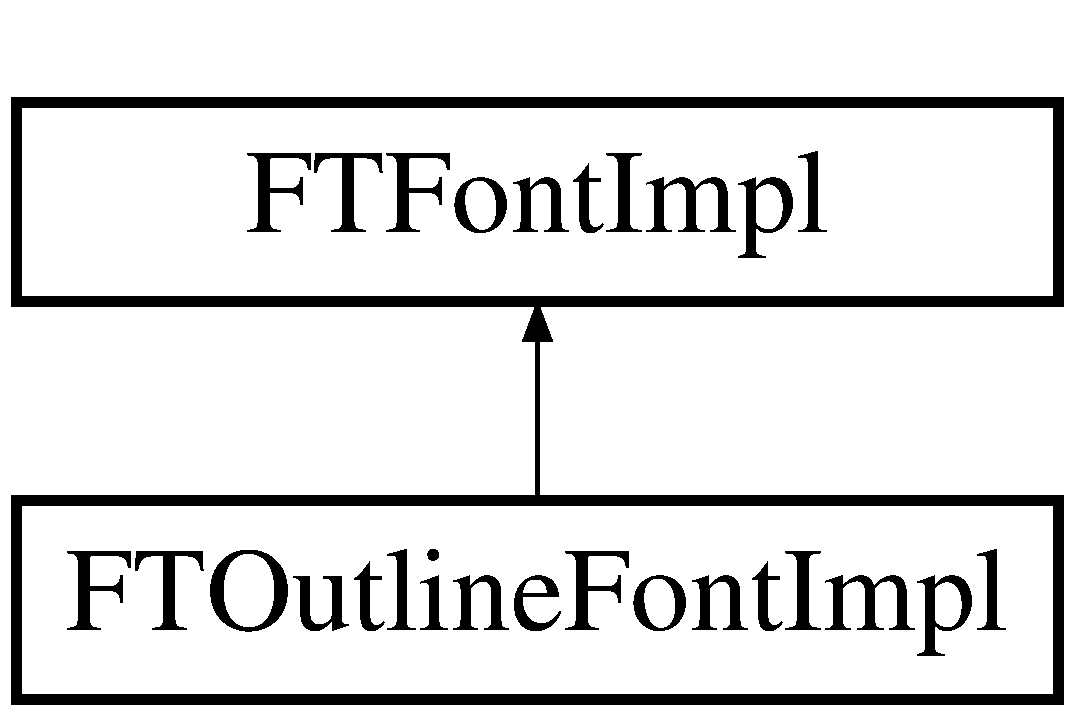
\includegraphics[height=2.000000cm]{class_f_t_outline_font_impl}
\end{center}
\end{figure}
\subsection*{Protected Member Functions}
\begin{DoxyCompactItemize}
\item 
\hypertarget{class_f_t_outline_font_impl_a01af1e37c082fce3f483361b455f9ac2}{
{\bfseries FTOutlineFontImpl} (FTFont $\ast$ftFont, const char $\ast$fontFilePath)}
\label{class_f_t_outline_font_impl_a01af1e37c082fce3f483361b455f9ac2}

\item 
\hypertarget{class_f_t_outline_font_impl_a3b0befb0c886bbc7cb8873afbfc0a9db}{
{\bfseries FTOutlineFontImpl} (FTFont $\ast$ftFont, const unsigned char $\ast$pBufferBytes, size\_\-t bufferSizeInBytes)}
\label{class_f_t_outline_font_impl_a3b0befb0c886bbc7cb8873afbfc0a9db}

\item 
virtual void \hyperlink{class_f_t_outline_font_impl_a22cb75a9c717403f399906d24d4aac82}{Outset} (float o)
\item 
\hypertarget{class_f_t_outline_font_impl_a10caae0ba62ba4c7d5a8742114517651}{
virtual FTPoint {\bfseries Render} (const char $\ast$s, const int len, FTPoint position, FTPoint spacing, int renderMode)}
\label{class_f_t_outline_font_impl_a10caae0ba62ba4c7d5a8742114517651}

\item 
\hypertarget{class_f_t_outline_font_impl_aa4957e338292c7202df9bfb1362e4084}{
virtual FTPoint {\bfseries Render} (const wchar\_\-t $\ast$s, const int len, FTPoint position, FTPoint spacing, int renderMode)}
\label{class_f_t_outline_font_impl_aa4957e338292c7202df9bfb1362e4084}

\end{DoxyCompactItemize}
\subsection*{Friends}
\begin{DoxyCompactItemize}
\item 
\hypertarget{class_f_t_outline_font_impl_a17f6eed308c6d1116a7f1d86010f6c9e}{
class {\bfseries FTOutlineFont}}
\label{class_f_t_outline_font_impl_a17f6eed308c6d1116a7f1d86010f6c9e}

\end{DoxyCompactItemize}


\subsection{Member Function Documentation}
\hypertarget{class_f_t_outline_font_impl_a22cb75a9c717403f399906d24d4aac82}{
\index{FTOutlineFontImpl@{FTOutlineFontImpl}!Outset@{Outset}}
\index{Outset@{Outset}!FTOutlineFontImpl@{FTOutlineFontImpl}}
\subsubsection[{Outset}]{\setlength{\rightskip}{0pt plus 5cm}virtual void FTOutlineFontImpl::Outset (
\begin{DoxyParamCaption}
\item[{float}]{ o}
\end{DoxyParamCaption}
)\hspace{0.3cm}{\ttfamily  \mbox{[}inline, protected, virtual\mbox{]}}}}
\label{class_f_t_outline_font_impl_a22cb75a9c717403f399906d24d4aac82}
Set the outset distance for the font. Only implemented by FTOutlineFont, FTPolygonFont and FTExtrudeFont


\begin{DoxyParams}{Parameters}
{\em outset} & The outset distance. \\
\hline
\end{DoxyParams}


Reimplemented from \hyperlink{class_f_t_font_impl}{FTFontImpl}.



The documentation for this class was generated from the following files:\begin{DoxyCompactItemize}
\item 
src/libs/FTGL/FTFont/FTOutlineFontImpl.h\item 
src/libs/FTGL/FTFont/FTOutlineFont.cpp\end{DoxyCompactItemize}

\hypertarget{class_f_t_outline_glyph_impl}{
\section{FTOutlineGlyphImpl Class Reference}
\label{class_f_t_outline_glyph_impl}\index{FTOutlineGlyphImpl@{FTOutlineGlyphImpl}}
}
Inheritance diagram for FTOutlineGlyphImpl:\begin{figure}[H]
\begin{center}
\leavevmode
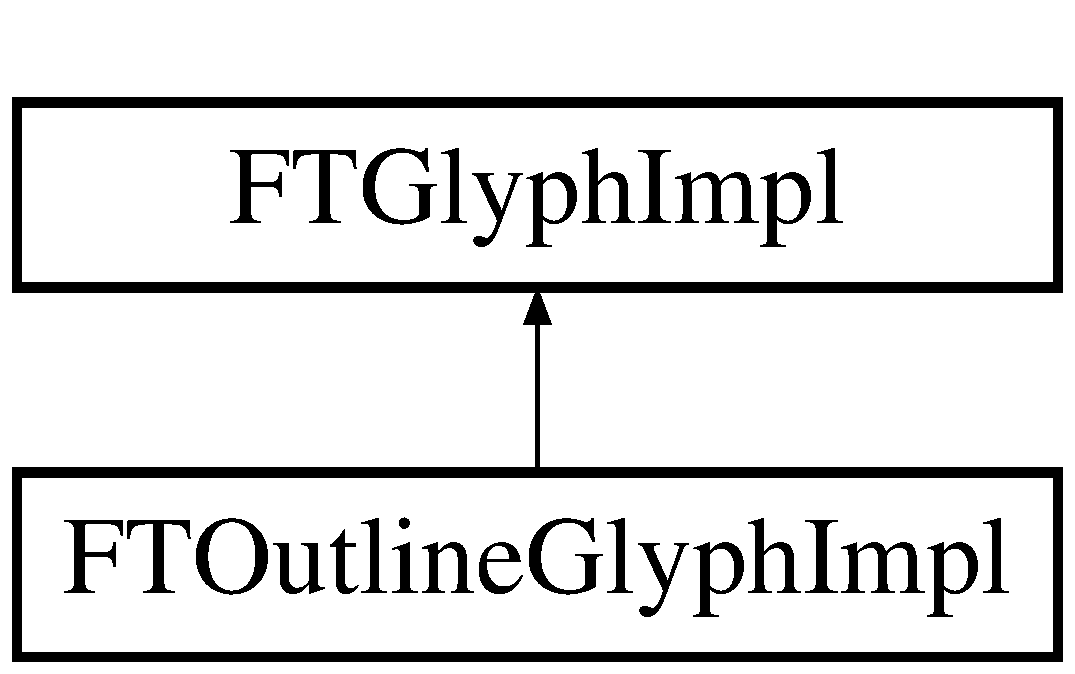
\includegraphics[height=2.000000cm]{class_f_t_outline_glyph_impl}
\end{center}
\end{figure}
\subsection*{Protected Member Functions}
\begin{DoxyCompactItemize}
\item 
\hypertarget{class_f_t_outline_glyph_impl_a0eac191ec3db6c8dbbf6956ded4342fa}{
{\bfseries FTOutlineGlyphImpl} (\hyperlink{struct_f_t___glyph_slot_rec__}{FT\_\-GlyphSlot} glyph, float outset, bool useDisplayList)}
\label{class_f_t_outline_glyph_impl_a0eac191ec3db6c8dbbf6956ded4342fa}

\item 
\hypertarget{class_f_t_outline_glyph_impl_a554ed38dfe9a113804394c35e9ef9d35}{
virtual const FTPoint \& {\bfseries RenderImpl} (const FTPoint \&pen, int renderMode)}
\label{class_f_t_outline_glyph_impl_a554ed38dfe9a113804394c35e9ef9d35}

\end{DoxyCompactItemize}
\subsection*{Friends}
\begin{DoxyCompactItemize}
\item 
\hypertarget{class_f_t_outline_glyph_impl_accb6ff0274a52a67e706edda49d6a201}{
class {\bfseries FTOutlineGlyph}}
\label{class_f_t_outline_glyph_impl_accb6ff0274a52a67e706edda49d6a201}

\end{DoxyCompactItemize}


The documentation for this class was generated from the following files:\begin{DoxyCompactItemize}
\item 
src/libs/FTGL/FTGlyph/FTOutlineGlyphImpl.h\item 
src/libs/FTGL/FTGlyph/FTOutlineGlyph.cpp\end{DoxyCompactItemize}

\hypertarget{class_f_t_pixmap_font_impl}{
\section{FTPixmapFontImpl Class Reference}
\label{class_f_t_pixmap_font_impl}\index{FTPixmapFontImpl@{FTPixmapFontImpl}}
}
Inheritance diagram for FTPixmapFontImpl:\begin{figure}[H]
\begin{center}
\leavevmode
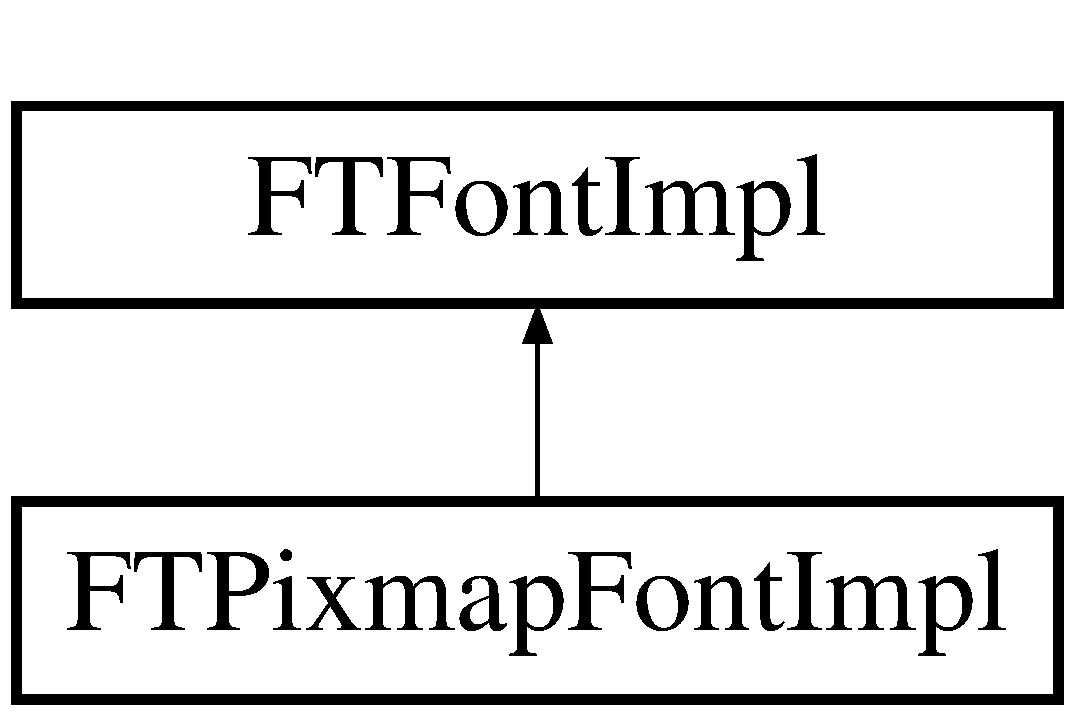
\includegraphics[height=2.000000cm]{class_f_t_pixmap_font_impl}
\end{center}
\end{figure}
\subsection*{Protected Member Functions}
\begin{DoxyCompactItemize}
\item 
\hypertarget{class_f_t_pixmap_font_impl_a08cfaf450bfbacce2b2d290b3d8d66d6}{
{\bfseries FTPixmapFontImpl} (FTFont $\ast$ftFont, const char $\ast$fontFilePath)}
\label{class_f_t_pixmap_font_impl_a08cfaf450bfbacce2b2d290b3d8d66d6}

\item 
\hypertarget{class_f_t_pixmap_font_impl_ac55c8ac1dffbd6559de73b44b85fde41}{
{\bfseries FTPixmapFontImpl} (FTFont $\ast$ftFont, const unsigned char $\ast$pBufferBytes, size\_\-t bufferSizeInBytes)}
\label{class_f_t_pixmap_font_impl_ac55c8ac1dffbd6559de73b44b85fde41}

\item 
\hypertarget{class_f_t_pixmap_font_impl_a3e2c75bd5cfa405a440735bcb83fa75f}{
virtual FTPoint {\bfseries Render} (const char $\ast$s, const int len, FTPoint position, FTPoint spacing, int renderMode)}
\label{class_f_t_pixmap_font_impl_a3e2c75bd5cfa405a440735bcb83fa75f}

\item 
\hypertarget{class_f_t_pixmap_font_impl_a95755217a2bf8d5d4a4a1f898fe1be73}{
virtual FTPoint {\bfseries Render} (const wchar\_\-t $\ast$s, const int len, FTPoint position, FTPoint spacing, int renderMode)}
\label{class_f_t_pixmap_font_impl_a95755217a2bf8d5d4a4a1f898fe1be73}

\end{DoxyCompactItemize}
\subsection*{Friends}
\begin{DoxyCompactItemize}
\item 
\hypertarget{class_f_t_pixmap_font_impl_ac7f382db9ff9f02888b67b7434d7edd4}{
class {\bfseries FTPixmapFont}}
\label{class_f_t_pixmap_font_impl_ac7f382db9ff9f02888b67b7434d7edd4}

\end{DoxyCompactItemize}


The documentation for this class was generated from the following files:\begin{DoxyCompactItemize}
\item 
src/libs/FTGL/FTFont/FTPixmapFontImpl.h\item 
src/libs/FTGL/FTFont/FTPixmapFont.cpp\end{DoxyCompactItemize}

\hypertarget{class_f_t_pixmap_glyph_impl}{
\section{FTPixmapGlyphImpl Class Reference}
\label{class_f_t_pixmap_glyph_impl}\index{FTPixmapGlyphImpl@{FTPixmapGlyphImpl}}
}
Inheritance diagram for FTPixmapGlyphImpl:\begin{figure}[H]
\begin{center}
\leavevmode
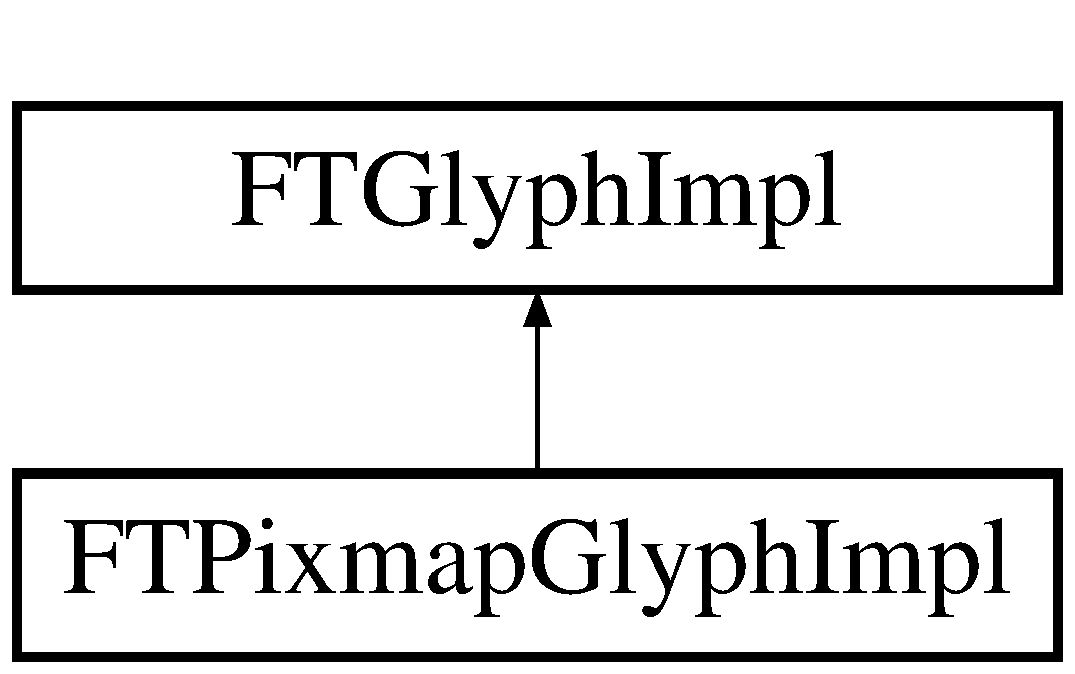
\includegraphics[height=2.000000cm]{class_f_t_pixmap_glyph_impl}
\end{center}
\end{figure}
\subsection*{Protected Member Functions}
\begin{DoxyCompactItemize}
\item 
\hypertarget{class_f_t_pixmap_glyph_impl_a65e1773b7c1f422abbccd90399cd3ec4}{
{\bfseries FTPixmapGlyphImpl} (\hyperlink{struct_f_t___glyph_slot_rec__}{FT\_\-GlyphSlot} glyph)}
\label{class_f_t_pixmap_glyph_impl_a65e1773b7c1f422abbccd90399cd3ec4}

\item 
\hypertarget{class_f_t_pixmap_glyph_impl_a9c5cf9105b59301f0b27cfa2350012c6}{
virtual const FTPoint \& {\bfseries RenderImpl} (const FTPoint \&pen, int renderMode)}
\label{class_f_t_pixmap_glyph_impl_a9c5cf9105b59301f0b27cfa2350012c6}

\end{DoxyCompactItemize}
\subsection*{Friends}
\begin{DoxyCompactItemize}
\item 
\hypertarget{class_f_t_pixmap_glyph_impl_ab141fccf761e39b9e4bec64cda0507a7}{
class {\bfseries FTPixmapGlyph}}
\label{class_f_t_pixmap_glyph_impl_ab141fccf761e39b9e4bec64cda0507a7}

\end{DoxyCompactItemize}


The documentation for this class was generated from the following files:\begin{DoxyCompactItemize}
\item 
src/libs/FTGL/FTGlyph/FTPixmapGlyphImpl.h\item 
src/libs/FTGL/FTGlyph/FTPixmapGlyph.cpp\end{DoxyCompactItemize}

\hypertarget{class_f_t_polygon_font_impl}{
\section{FTPolygonFontImpl Class Reference}
\label{class_f_t_polygon_font_impl}\index{FTPolygonFontImpl@{FTPolygonFontImpl}}
}
Inheritance diagram for FTPolygonFontImpl:\begin{figure}[H]
\begin{center}
\leavevmode
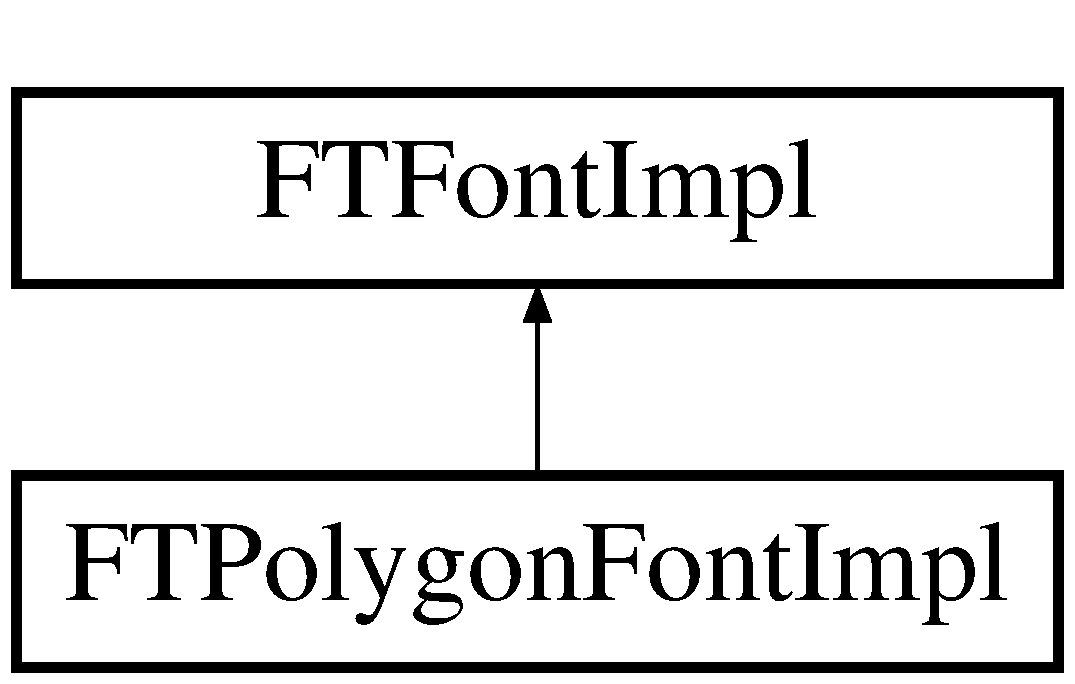
\includegraphics[height=2.000000cm]{class_f_t_polygon_font_impl}
\end{center}
\end{figure}
\subsection*{Protected Member Functions}
\begin{DoxyCompactItemize}
\item 
\hypertarget{class_f_t_polygon_font_impl_adbe87469ee12af1a0a1b7999ede7cc98}{
{\bfseries FTPolygonFontImpl} (FTFont $\ast$ftFont, const char $\ast$fontFilePath)}
\label{class_f_t_polygon_font_impl_adbe87469ee12af1a0a1b7999ede7cc98}

\item 
\hypertarget{class_f_t_polygon_font_impl_a140310c1898543ff1dec5865841b630b}{
{\bfseries FTPolygonFontImpl} (FTFont $\ast$ftFont, const unsigned char $\ast$pBufferBytes, size\_\-t bufferSizeInBytes)}
\label{class_f_t_polygon_font_impl_a140310c1898543ff1dec5865841b630b}

\item 
virtual void \hyperlink{class_f_t_polygon_font_impl_ac565010b774c7ddb84db28b422ea9b3e}{Outset} (float o)
\end{DoxyCompactItemize}
\subsection*{Friends}
\begin{DoxyCompactItemize}
\item 
\hypertarget{class_f_t_polygon_font_impl_abd1c273c43e47346ad6c178ec173cc41}{
class {\bfseries FTPolygonFont}}
\label{class_f_t_polygon_font_impl_abd1c273c43e47346ad6c178ec173cc41}

\end{DoxyCompactItemize}


\subsection{Member Function Documentation}
\hypertarget{class_f_t_polygon_font_impl_ac565010b774c7ddb84db28b422ea9b3e}{
\index{FTPolygonFontImpl@{FTPolygonFontImpl}!Outset@{Outset}}
\index{Outset@{Outset}!FTPolygonFontImpl@{FTPolygonFontImpl}}
\subsubsection[{Outset}]{\setlength{\rightskip}{0pt plus 5cm}virtual void FTPolygonFontImpl::Outset (
\begin{DoxyParamCaption}
\item[{float}]{ o}
\end{DoxyParamCaption}
)\hspace{0.3cm}{\ttfamily  \mbox{[}inline, protected, virtual\mbox{]}}}}
\label{class_f_t_polygon_font_impl_ac565010b774c7ddb84db28b422ea9b3e}
Set the outset distance for the font. Only implemented by FTOutlineFont, FTPolygonFont and FTExtrudeFont


\begin{DoxyParams}{Parameters}
{\em depth} & The outset distance. \\
\hline
\end{DoxyParams}


Reimplemented from \hyperlink{class_f_t_font_impl}{FTFontImpl}.



The documentation for this class was generated from the following files:\begin{DoxyCompactItemize}
\item 
src/libs/FTGL/FTFont/FTPolygonFontImpl.h\item 
src/libs/FTGL/FTFont/FTPolygonFont.cpp\end{DoxyCompactItemize}

\hypertarget{class_f_t_polygon_glyph_impl}{
\section{FTPolygonGlyphImpl Class Reference}
\label{class_f_t_polygon_glyph_impl}\index{FTPolygonGlyphImpl@{FTPolygonGlyphImpl}}
}
Inheritance diagram for FTPolygonGlyphImpl:\begin{figure}[H]
\begin{center}
\leavevmode
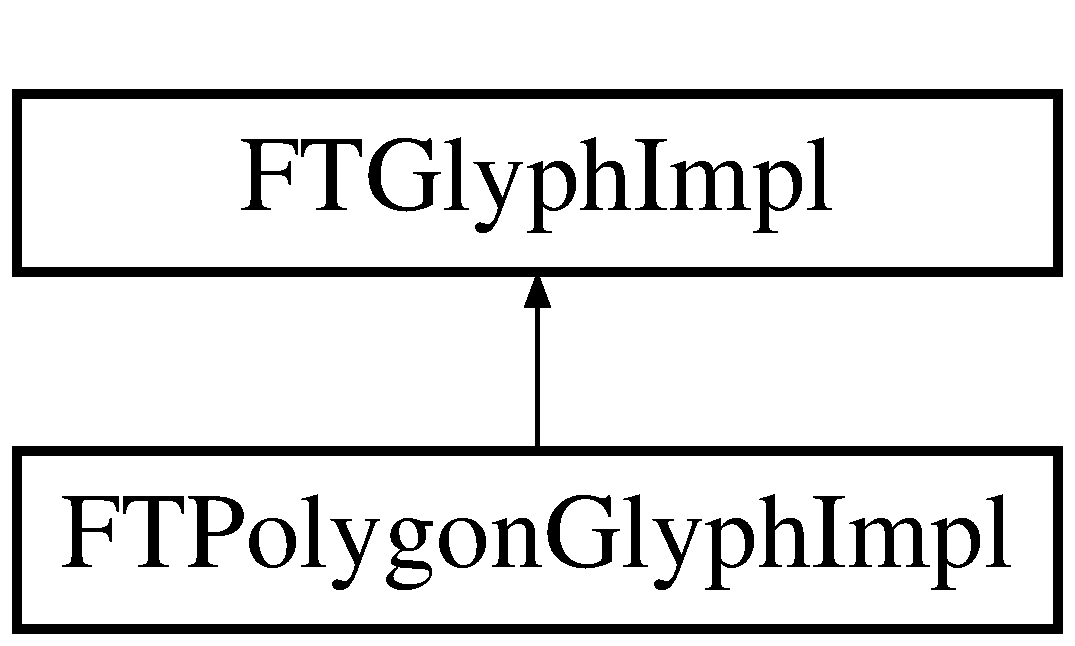
\includegraphics[height=2.000000cm]{class_f_t_polygon_glyph_impl}
\end{center}
\end{figure}
\subsection*{Public Member Functions}
\begin{DoxyCompactItemize}
\item 
\hypertarget{class_f_t_polygon_glyph_impl_ab302277a0e76adf9570f1ef9f9ae851f}{
{\bfseries FTPolygonGlyphImpl} (\hyperlink{struct_f_t___glyph_slot_rec__}{FT\_\-GlyphSlot} glyph, float outset, bool useDisplayList)}
\label{class_f_t_polygon_glyph_impl_ab302277a0e76adf9570f1ef9f9ae851f}

\item 
\hypertarget{class_f_t_polygon_glyph_impl_af689ff9cecc738d292d494bf83adca39}{
virtual const FTPoint \& {\bfseries RenderImpl} (const FTPoint \&pen, int renderMode)}
\label{class_f_t_polygon_glyph_impl_af689ff9cecc738d292d494bf83adca39}

\end{DoxyCompactItemize}
\subsection*{Friends}
\begin{DoxyCompactItemize}
\item 
\hypertarget{class_f_t_polygon_glyph_impl_a0e33f7bc34e1097f8f9adcb6252d1bc0}{
class {\bfseries FTPolygonGlyph}}
\label{class_f_t_polygon_glyph_impl_a0e33f7bc34e1097f8f9adcb6252d1bc0}

\end{DoxyCompactItemize}


The documentation for this class was generated from the following files:\begin{DoxyCompactItemize}
\item 
src/libs/FTGL/FTGlyph/FTPolygonGlyphImpl.h\item 
src/libs/FTGL/FTGlyph/FTPolygonGlyph.cpp\end{DoxyCompactItemize}

\hypertarget{class_f_t_simple_layout_impl}{
\section{FTSimpleLayoutImpl Class Reference}
\label{class_f_t_simple_layout_impl}\index{FTSimpleLayoutImpl@{FTSimpleLayoutImpl}}
}
Inheritance diagram for FTSimpleLayoutImpl:\begin{figure}[H]
\begin{center}
\leavevmode
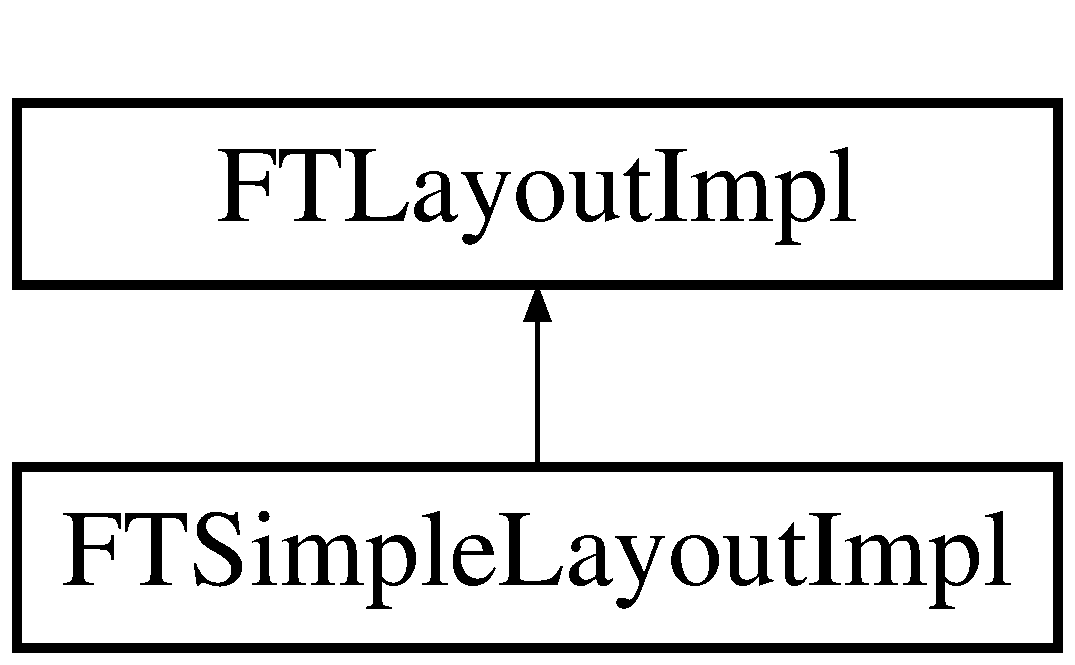
\includegraphics[height=2.000000cm]{class_f_t_simple_layout_impl}
\end{center}
\end{figure}
\subsection*{Protected Member Functions}
\begin{DoxyCompactItemize}
\item 
\hypertarget{class_f_t_simple_layout_impl_a6cdedbc1045881dcb3ddedea054a7987}{
virtual FTBBox {\bfseries BBox} (const char $\ast$string, const int len, FTPoint position)}
\label{class_f_t_simple_layout_impl_a6cdedbc1045881dcb3ddedea054a7987}

\item 
\hypertarget{class_f_t_simple_layout_impl_a682650a15a67eb182b2de9e7001875cb}{
virtual FTBBox {\bfseries BBox} (const wchar\_\-t $\ast$string, const int len, FTPoint position)}
\label{class_f_t_simple_layout_impl_a682650a15a67eb182b2de9e7001875cb}

\item 
\hypertarget{class_f_t_simple_layout_impl_abfe85f44b3d4a2f8691b5e11ab26828a}{
virtual void {\bfseries Render} (const char $\ast$string, const int len, FTPoint position, int renderMode)}
\label{class_f_t_simple_layout_impl_abfe85f44b3d4a2f8691b5e11ab26828a}

\item 
\hypertarget{class_f_t_simple_layout_impl_ac69f1a3cdac5e6dd692b547df3f77825}{
virtual void {\bfseries Render} (const wchar\_\-t $\ast$string, const int len, FTPoint position, int renderMode)}
\label{class_f_t_simple_layout_impl_ac69f1a3cdac5e6dd692b547df3f77825}

\item 
virtual void \hyperlink{class_f_t_simple_layout_impl_abdbd064c650f1e17d2bd3139536aff47}{RenderSpace} (const char $\ast$string, const int len, FTPoint position, int renderMode, const float extraSpace)
\item 
virtual void \hyperlink{class_f_t_simple_layout_impl_a6b5334d053e9c79dd459f8b88c0e60a4}{RenderSpace} (const wchar\_\-t $\ast$string, const int len, FTPoint position, int renderMode, const float extraSpace)
\end{DoxyCompactItemize}
\subsection*{Friends}
\begin{DoxyCompactItemize}
\item 
\hypertarget{class_f_t_simple_layout_impl_ae27eaa779922d14c8eb0f476456c7099}{
class {\bfseries FTSimpleLayout}}
\label{class_f_t_simple_layout_impl_ae27eaa779922d14c8eb0f476456c7099}

\end{DoxyCompactItemize}


\subsection{Member Function Documentation}
\hypertarget{class_f_t_simple_layout_impl_a6b5334d053e9c79dd459f8b88c0e60a4}{
\index{FTSimpleLayoutImpl@{FTSimpleLayoutImpl}!RenderSpace@{RenderSpace}}
\index{RenderSpace@{RenderSpace}!FTSimpleLayoutImpl@{FTSimpleLayoutImpl}}
\subsubsection[{RenderSpace}]{\setlength{\rightskip}{0pt plus 5cm}void FTSimpleLayoutImpl::RenderSpace (
\begin{DoxyParamCaption}
\item[{const wchar\_\-t $\ast$}]{ string, }
\item[{const int}]{ len, }
\item[{FTPoint}]{ position, }
\item[{int}]{ renderMode, }
\item[{const float}]{ extraSpace}
\end{DoxyParamCaption}
)\hspace{0.3cm}{\ttfamily  \mbox{[}protected, virtual\mbox{]}}}}
\label{class_f_t_simple_layout_impl_a6b5334d053e9c79dd459f8b88c0e60a4}
Render a string of characters and distribute extra space amongst the whitespace regions of the string.


\begin{DoxyParams}{Parameters}
{\em string} & A buffer of wchar\_\-t characters to output. \\
\hline
{\em len} & The length of the string. If $<$ 0 then all characters will be displayed until a null character is encountered. \\
\hline
{\em position} & TODO \\
\hline
{\em renderMode} & Render mode to display \\
\hline
{\em extraSpace} & The amount of extra space to distribute amongst the characters. \\
\hline
\end{DoxyParams}
\hypertarget{class_f_t_simple_layout_impl_abdbd064c650f1e17d2bd3139536aff47}{
\index{FTSimpleLayoutImpl@{FTSimpleLayoutImpl}!RenderSpace@{RenderSpace}}
\index{RenderSpace@{RenderSpace}!FTSimpleLayoutImpl@{FTSimpleLayoutImpl}}
\subsubsection[{RenderSpace}]{\setlength{\rightskip}{0pt plus 5cm}void FTSimpleLayoutImpl::RenderSpace (
\begin{DoxyParamCaption}
\item[{const char $\ast$}]{ string, }
\item[{const int}]{ len, }
\item[{FTPoint}]{ position, }
\item[{int}]{ renderMode, }
\item[{const float}]{ extraSpace}
\end{DoxyParamCaption}
)\hspace{0.3cm}{\ttfamily  \mbox{[}protected, virtual\mbox{]}}}}
\label{class_f_t_simple_layout_impl_abdbd064c650f1e17d2bd3139536aff47}
Render a string of characters and distribute extra space amongst the whitespace regions of the string.


\begin{DoxyParams}{Parameters}
{\em string} & A buffer of wchar\_\-t characters to output. \\
\hline
{\em len} & The length of the string. If $<$ 0 then all characters will be displayed until a null character is encountered. \\
\hline
{\em position} & TODO \\
\hline
{\em renderMode} & Render mode to display \\
\hline
{\em extraSpace} & The amount of extra space to distribute amongst the characters. \\
\hline
\end{DoxyParams}


The documentation for this class was generated from the following files:\begin{DoxyCompactItemize}
\item 
src/libs/FTGL/FTLayout/FTSimpleLayoutImpl.h\item 
src/libs/FTGL/FTLayout/FTSimpleLayout.cpp\end{DoxyCompactItemize}

\hypertarget{class_f_t_size}{
\section{FTSize Class Reference}
\label{class_f_t_size}\index{FTSize@{FTSize}}
}


{\ttfamily \#include $<$FTSize.h$>$}

\subsection*{Public Member Functions}
\begin{DoxyCompactItemize}
\item 
\hyperlink{class_f_t_size_ae1b459031c2ab7fe6ef98530c0251700}{FTSize} ()
\item 
virtual \hyperlink{class_f_t_size_a7bf23332d879f3e9d76675290012b275}{$\sim$FTSize} ()
\item 
bool \hyperlink{class_f_t_size_a15c6c82655544d1edb101e00e42ffad9}{CharSize} (\hyperlink{struct_f_t___face_rec__}{FT\_\-Face} $\ast$face, unsigned int point\_\-size, unsigned int x\_\-resolution, unsigned int y\_\-resolution)
\item 
unsigned int \hyperlink{class_f_t_size_a489fba0a722afd8dfa2a67142cd51767}{CharSize} () const 
\item 
float \hyperlink{class_f_t_size_a7865c27cb979feace5ccce2fb544a490}{Ascender} () const 
\item 
float \hyperlink{class_f_t_size_a75c1b86d32c5ea1d296234edb1e4b7ab}{Descender} () const 
\item 
float \hyperlink{class_f_t_size_af0e7398f27936ffe4cbed04c3cfa889d}{Height} () const 
\item 
float \hyperlink{class_f_t_size_a8fe639fa29815a89cdd84138b2564840}{Width} () const 
\item 
float \hyperlink{class_f_t_size_ab85fb58156a855d01b5a4e9e1b91e0e2}{Underline} () const 
\item 
FT\_\-Error \hyperlink{class_f_t_size_a990a2df40c9c1ed06db8d34b2ac3580b}{Error} () const 
\end{DoxyCompactItemize}


\subsection{Detailed Description}
\hyperlink{class_f_t_size}{FTSize} class provides an abstraction layer for the Freetype Size.

\begin{DoxySeeAlso}{See also}
\char`\"{}Freetype 2 Documentation\char`\"{} 
\end{DoxySeeAlso}


\subsection{Constructor \& Destructor Documentation}
\hypertarget{class_f_t_size_ae1b459031c2ab7fe6ef98530c0251700}{
\index{FTSize@{FTSize}!FTSize@{FTSize}}
\index{FTSize@{FTSize}!FTSize@{FTSize}}
\subsubsection[{FTSize}]{\setlength{\rightskip}{0pt plus 5cm}FTSize::FTSize (
\begin{DoxyParamCaption}
{}
\end{DoxyParamCaption}
)}}
\label{class_f_t_size_ae1b459031c2ab7fe6ef98530c0251700}
Default Constructor \hypertarget{class_f_t_size_a7bf23332d879f3e9d76675290012b275}{
\index{FTSize@{FTSize}!$\sim$FTSize@{$\sim$FTSize}}
\index{$\sim$FTSize@{$\sim$FTSize}!FTSize@{FTSize}}
\subsubsection[{$\sim$FTSize}]{\setlength{\rightskip}{0pt plus 5cm}FTSize::$\sim$FTSize (
\begin{DoxyParamCaption}
{}
\end{DoxyParamCaption}
)\hspace{0.3cm}{\ttfamily  \mbox{[}virtual\mbox{]}}}}
\label{class_f_t_size_a7bf23332d879f3e9d76675290012b275}
Destructor 

\subsection{Member Function Documentation}
\hypertarget{class_f_t_size_a7865c27cb979feace5ccce2fb544a490}{
\index{FTSize@{FTSize}!Ascender@{Ascender}}
\index{Ascender@{Ascender}!FTSize@{FTSize}}
\subsubsection[{Ascender}]{\setlength{\rightskip}{0pt plus 5cm}float FTSize::Ascender (
\begin{DoxyParamCaption}
{}
\end{DoxyParamCaption}
) const}}
\label{class_f_t_size_a7865c27cb979feace5ccce2fb544a490}
Gets the global ascender height for the face in pixels.

\begin{DoxyReturn}{Returns}
Ascender height 
\end{DoxyReturn}
\hypertarget{class_f_t_size_a489fba0a722afd8dfa2a67142cd51767}{
\index{FTSize@{FTSize}!CharSize@{CharSize}}
\index{CharSize@{CharSize}!FTSize@{FTSize}}
\subsubsection[{CharSize}]{\setlength{\rightskip}{0pt plus 5cm}unsigned int FTSize::CharSize (
\begin{DoxyParamCaption}
{}
\end{DoxyParamCaption}
) const}}
\label{class_f_t_size_a489fba0a722afd8dfa2a67142cd51767}
get the char size for the current face.

\begin{DoxyReturn}{Returns}
The char size in points 
\end{DoxyReturn}
\hypertarget{class_f_t_size_a15c6c82655544d1edb101e00e42ffad9}{
\index{FTSize@{FTSize}!CharSize@{CharSize}}
\index{CharSize@{CharSize}!FTSize@{FTSize}}
\subsubsection[{CharSize}]{\setlength{\rightskip}{0pt plus 5cm}bool FTSize::CharSize (
\begin{DoxyParamCaption}
\item[{{\bf FT\_\-Face} $\ast$}]{ face, }
\item[{unsigned int}]{ point\_\-size, }
\item[{unsigned int}]{ x\_\-resolution, }
\item[{unsigned int}]{ y\_\-resolution}
\end{DoxyParamCaption}
)}}
\label{class_f_t_size_a15c6c82655544d1edb101e00e42ffad9}
Sets the char size for the current face.

This doesn't guarantee that the size was set correctly. Clients should check errors. If an error does occur the size object isn't modified.


\begin{DoxyParams}{Parameters}
{\em face} & Parent face for this size object \\
\hline
{\em point\_\-size} & the face size in points (1/72 inch) \\
\hline
{\em x\_\-resolution} & the horizontal resolution of the target device. \\
\hline
{\em y\_\-resolution} & the vertical resolution of the target device. \\
\hline
\end{DoxyParams}
\begin{DoxyReturn}{Returns}
{\ttfamily true} if the size has been set. Clients should check \hyperlink{class_f_t_size_a990a2df40c9c1ed06db8d34b2ac3580b}{Error()} for more information if this function returns false() 
\end{DoxyReturn}
\hypertarget{class_f_t_size_a75c1b86d32c5ea1d296234edb1e4b7ab}{
\index{FTSize@{FTSize}!Descender@{Descender}}
\index{Descender@{Descender}!FTSize@{FTSize}}
\subsubsection[{Descender}]{\setlength{\rightskip}{0pt plus 5cm}float FTSize::Descender (
\begin{DoxyParamCaption}
{}
\end{DoxyParamCaption}
) const}}
\label{class_f_t_size_a75c1b86d32c5ea1d296234edb1e4b7ab}
Gets the global descender height for the face in pixels.

\begin{DoxyReturn}{Returns}
Ascender height 
\end{DoxyReturn}
\hypertarget{class_f_t_size_a990a2df40c9c1ed06db8d34b2ac3580b}{
\index{FTSize@{FTSize}!Error@{Error}}
\index{Error@{Error}!FTSize@{FTSize}}
\subsubsection[{Error}]{\setlength{\rightskip}{0pt plus 5cm}FT\_\-Error FTSize::Error (
\begin{DoxyParamCaption}
{}
\end{DoxyParamCaption}
) const\hspace{0.3cm}{\ttfamily  \mbox{[}inline\mbox{]}}}}
\label{class_f_t_size_a990a2df40c9c1ed06db8d34b2ac3580b}
Queries for errors.

\begin{DoxyReturn}{Returns}
The current error code. 
\end{DoxyReturn}
\hypertarget{class_f_t_size_af0e7398f27936ffe4cbed04c3cfa889d}{
\index{FTSize@{FTSize}!Height@{Height}}
\index{Height@{Height}!FTSize@{FTSize}}
\subsubsection[{Height}]{\setlength{\rightskip}{0pt plus 5cm}float FTSize::Height (
\begin{DoxyParamCaption}
{}
\end{DoxyParamCaption}
) const}}
\label{class_f_t_size_af0e7398f27936ffe4cbed04c3cfa889d}
Gets the global face height for the face.

If the face is scalable this returns the height of the global bounding box which ensures that any glyph will be less than or equal to this height. If the font isn't scalable there is no guarantee that glyphs will not be taller than this value.

\begin{DoxyReturn}{Returns}
height in pixels. 
\end{DoxyReturn}
\hypertarget{class_f_t_size_ab85fb58156a855d01b5a4e9e1b91e0e2}{
\index{FTSize@{FTSize}!Underline@{Underline}}
\index{Underline@{Underline}!FTSize@{FTSize}}
\subsubsection[{Underline}]{\setlength{\rightskip}{0pt plus 5cm}float FTSize::Underline (
\begin{DoxyParamCaption}
{}
\end{DoxyParamCaption}
) const}}
\label{class_f_t_size_ab85fb58156a855d01b5a4e9e1b91e0e2}
Gets the underline position for the face.

\begin{DoxyReturn}{Returns}
underline position in pixels 
\end{DoxyReturn}
\hypertarget{class_f_t_size_a8fe639fa29815a89cdd84138b2564840}{
\index{FTSize@{FTSize}!Width@{Width}}
\index{Width@{Width}!FTSize@{FTSize}}
\subsubsection[{Width}]{\setlength{\rightskip}{0pt plus 5cm}float FTSize::Width (
\begin{DoxyParamCaption}
{}
\end{DoxyParamCaption}
) const}}
\label{class_f_t_size_a8fe639fa29815a89cdd84138b2564840}
Gets the global face width for the face.

If the face is scalable this returns the width of the global bounding box which ensures that any glyph will be less than or equal to this width. If the font isn't scalable this value is the max\_\-advance for the face.

\begin{DoxyReturn}{Returns}
width in pixels. 
\end{DoxyReturn}


The documentation for this class was generated from the following files:\begin{DoxyCompactItemize}
\item 
src/libs/FTGL/FTSize.h\item 
src/libs/FTGL/FTSize.cpp\end{DoxyCompactItemize}

\hypertarget{class_f_t_tesselation}{
\section{FTTesselation Class Reference}
\label{class_f_t_tesselation}\index{FTTesselation@{FTTesselation}}
}


{\ttfamily \#include $<$FTVectoriser.h$>$}

\subsection*{Public Member Functions}
\begin{DoxyCompactItemize}
\item 
\hyperlink{class_f_t_tesselation_a8ae81852ffa0dfb1bc65e85dc6d35df2}{FTTesselation} (GLenum m)
\item 
\hyperlink{class_f_t_tesselation_a55bd008edbf969720fa3dc083bce1ac0}{$\sim$FTTesselation} ()
\item 
void \hyperlink{class_f_t_tesselation_a204a9e646cee25f374faad125d71d5e6}{AddPoint} (const FTGL\_\-DOUBLE x, const FTGL\_\-DOUBLE y, const FTGL\_\-DOUBLE z)
\item 
size\_\-t \hyperlink{class_f_t_tesselation_aa3cb26a53c3534576339f946acdc0cc7}{PointCount} () const 
\item 
\hypertarget{class_f_t_tesselation_a964ae8f16f216ca545f44a087f31e827}{
const FTPoint \& {\bfseries Point} (unsigned int index) const }
\label{class_f_t_tesselation_a964ae8f16f216ca545f44a087f31e827}

\item 
GLenum \hyperlink{class_f_t_tesselation_a06c290061a75bad0d38a2d5b2f6b09a1}{PolygonType} () const 
\end{DoxyCompactItemize}


\subsection{Detailed Description}
\hyperlink{class_f_t_tesselation}{FTTesselation} captures points that are output by OpenGL's gluTesselator. 

\subsection{Constructor \& Destructor Documentation}
\hypertarget{class_f_t_tesselation_a8ae81852ffa0dfb1bc65e85dc6d35df2}{
\index{FTTesselation@{FTTesselation}!FTTesselation@{FTTesselation}}
\index{FTTesselation@{FTTesselation}!FTTesselation@{FTTesselation}}
\subsubsection[{FTTesselation}]{\setlength{\rightskip}{0pt plus 5cm}FTTesselation::FTTesselation (
\begin{DoxyParamCaption}
\item[{GLenum}]{ m}
\end{DoxyParamCaption}
)\hspace{0.3cm}{\ttfamily  \mbox{[}inline\mbox{]}}}}
\label{class_f_t_tesselation_a8ae81852ffa0dfb1bc65e85dc6d35df2}
Default constructor \hypertarget{class_f_t_tesselation_a55bd008edbf969720fa3dc083bce1ac0}{
\index{FTTesselation@{FTTesselation}!$\sim$FTTesselation@{$\sim$FTTesselation}}
\index{$\sim$FTTesselation@{$\sim$FTTesselation}!FTTesselation@{FTTesselation}}
\subsubsection[{$\sim$FTTesselation}]{\setlength{\rightskip}{0pt plus 5cm}FTTesselation::$\sim$FTTesselation (
\begin{DoxyParamCaption}
{}
\end{DoxyParamCaption}
)\hspace{0.3cm}{\ttfamily  \mbox{[}inline\mbox{]}}}}
\label{class_f_t_tesselation_a55bd008edbf969720fa3dc083bce1ac0}
Destructor 

\subsection{Member Function Documentation}
\hypertarget{class_f_t_tesselation_a204a9e646cee25f374faad125d71d5e6}{
\index{FTTesselation@{FTTesselation}!AddPoint@{AddPoint}}
\index{AddPoint@{AddPoint}!FTTesselation@{FTTesselation}}
\subsubsection[{AddPoint}]{\setlength{\rightskip}{0pt plus 5cm}void FTTesselation::AddPoint (
\begin{DoxyParamCaption}
\item[{const FTGL\_\-DOUBLE}]{ x, }
\item[{const FTGL\_\-DOUBLE}]{ y, }
\item[{const FTGL\_\-DOUBLE}]{ z}
\end{DoxyParamCaption}
)\hspace{0.3cm}{\ttfamily  \mbox{[}inline\mbox{]}}}}
\label{class_f_t_tesselation_a204a9e646cee25f374faad125d71d5e6}
Add a point to the mesh. \hypertarget{class_f_t_tesselation_aa3cb26a53c3534576339f946acdc0cc7}{
\index{FTTesselation@{FTTesselation}!PointCount@{PointCount}}
\index{PointCount@{PointCount}!FTTesselation@{FTTesselation}}
\subsubsection[{PointCount}]{\setlength{\rightskip}{0pt plus 5cm}size\_\-t FTTesselation::PointCount (
\begin{DoxyParamCaption}
{}
\end{DoxyParamCaption}
) const\hspace{0.3cm}{\ttfamily  \mbox{[}inline\mbox{]}}}}
\label{class_f_t_tesselation_aa3cb26a53c3534576339f946acdc0cc7}
The number of points in this mesh \hypertarget{class_f_t_tesselation_a06c290061a75bad0d38a2d5b2f6b09a1}{
\index{FTTesselation@{FTTesselation}!PolygonType@{PolygonType}}
\index{PolygonType@{PolygonType}!FTTesselation@{FTTesselation}}
\subsubsection[{PolygonType}]{\setlength{\rightskip}{0pt plus 5cm}GLenum FTTesselation::PolygonType (
\begin{DoxyParamCaption}
{}
\end{DoxyParamCaption}
) const\hspace{0.3cm}{\ttfamily  \mbox{[}inline\mbox{]}}}}
\label{class_f_t_tesselation_a06c290061a75bad0d38a2d5b2f6b09a1}
Return the OpenGL polygon type. 

The documentation for this class was generated from the following file:\begin{DoxyCompactItemize}
\item 
src/libs/FTGL/FTVectoriser.h\end{DoxyCompactItemize}

\hypertarget{class_f_t_texture_font_impl}{
\section{FTTextureFontImpl Class Reference}
\label{class_f_t_texture_font_impl}\index{FTTextureFontImpl@{FTTextureFontImpl}}
}
Inheritance diagram for FTTextureFontImpl:\begin{figure}[H]
\begin{center}
\leavevmode
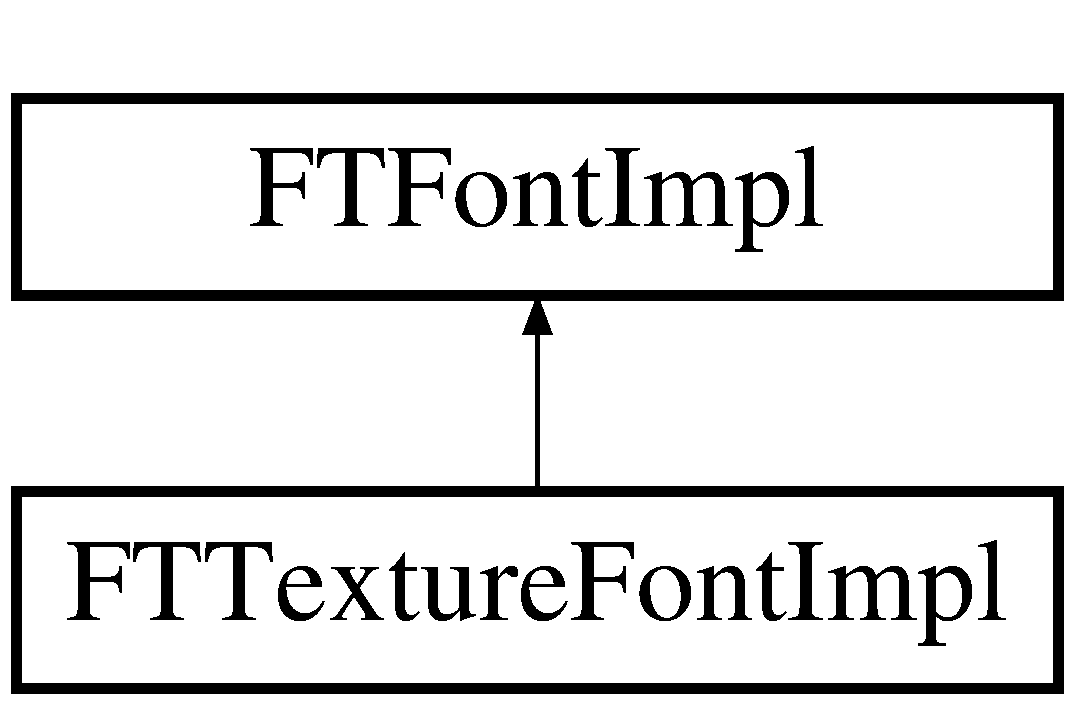
\includegraphics[height=2.000000cm]{class_f_t_texture_font_impl}
\end{center}
\end{figure}
\subsection*{Protected Member Functions}
\begin{DoxyCompactItemize}
\item 
\hypertarget{class_f_t_texture_font_impl_a6e5537e5ce6f58e8f8244c9d0cd44d9f}{
{\bfseries FTTextureFontImpl} (FTFont $\ast$ftFont, const char $\ast$fontFilePath)}
\label{class_f_t_texture_font_impl_a6e5537e5ce6f58e8f8244c9d0cd44d9f}

\item 
\hypertarget{class_f_t_texture_font_impl_a4554181466170efa12b9a12e4936b61d}{
{\bfseries FTTextureFontImpl} (FTFont $\ast$ftFont, const unsigned char $\ast$pBufferBytes, size\_\-t bufferSizeInBytes)}
\label{class_f_t_texture_font_impl_a4554181466170efa12b9a12e4936b61d}

\item 
virtual bool \hyperlink{class_f_t_texture_font_impl_ac5ccaca6cc8a53292b5028a629e49244}{FaceSize} (const unsigned int size, const unsigned int res=72)
\item 
\hypertarget{class_f_t_texture_font_impl_a8b53cbe2b70ad38af59a7d79945122d9}{
virtual FTPoint {\bfseries Render} (const char $\ast$s, const int len, FTPoint position, FTPoint spacing, int renderMode)}
\label{class_f_t_texture_font_impl_a8b53cbe2b70ad38af59a7d79945122d9}

\item 
\hypertarget{class_f_t_texture_font_impl_aba852ac4cc9b759073b6370e059e6c11}{
virtual FTPoint {\bfseries Render} (const wchar\_\-t $\ast$s, const int len, FTPoint position, FTPoint spacing, int renderMode)}
\label{class_f_t_texture_font_impl_aba852ac4cc9b759073b6370e059e6c11}

\end{DoxyCompactItemize}
\subsection*{Friends}
\begin{DoxyCompactItemize}
\item 
\hypertarget{class_f_t_texture_font_impl_a7870c341f7269dfae257e93406c17c92}{
class {\bfseries FTTextureFont}}
\label{class_f_t_texture_font_impl_a7870c341f7269dfae257e93406c17c92}

\end{DoxyCompactItemize}


\subsection{Member Function Documentation}
\hypertarget{class_f_t_texture_font_impl_ac5ccaca6cc8a53292b5028a629e49244}{
\index{FTTextureFontImpl@{FTTextureFontImpl}!FaceSize@{FaceSize}}
\index{FaceSize@{FaceSize}!FTTextureFontImpl@{FTTextureFontImpl}}
\subsubsection[{FaceSize}]{\setlength{\rightskip}{0pt plus 5cm}bool FTTextureFontImpl::FaceSize (
\begin{DoxyParamCaption}
\item[{const unsigned int}]{ size, }
\item[{const unsigned int}]{ res = {\ttfamily 72}}
\end{DoxyParamCaption}
)\hspace{0.3cm}{\ttfamily  \mbox{[}protected, virtual\mbox{]}}}}
\label{class_f_t_texture_font_impl_ac5ccaca6cc8a53292b5028a629e49244}
Set the char size for the current face.


\begin{DoxyParams}{Parameters}
{\em size} & the face size in points (1/72 inch) \\
\hline
{\em res} & the resolution of the target device. \\
\hline
\end{DoxyParams}
\begin{DoxyReturn}{Returns}
{\ttfamily true} if size was set correctly 
\end{DoxyReturn}


Reimplemented from \hyperlink{class_f_t_font_impl}{FTFontImpl}.



The documentation for this class was generated from the following files:\begin{DoxyCompactItemize}
\item 
src/libs/FTGL/FTFont/FTTextureFontImpl.h\item 
src/libs/FTGL/FTFont/FTTextureFont.cpp\end{DoxyCompactItemize}

\hypertarget{class_f_t_texture_glyph_impl}{
\section{FTTextureGlyphImpl Class Reference}
\label{class_f_t_texture_glyph_impl}\index{FTTextureGlyphImpl@{FTTextureGlyphImpl}}
}
Inheritance diagram for FTTextureGlyphImpl:\begin{figure}[H]
\begin{center}
\leavevmode
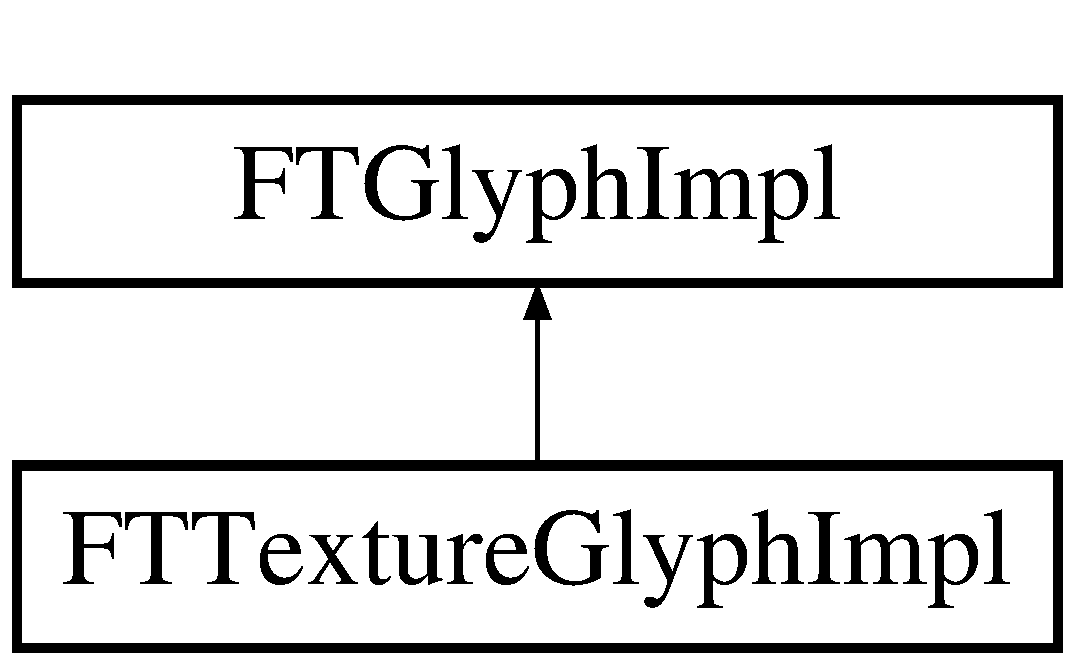
\includegraphics[height=2.000000cm]{class_f_t_texture_glyph_impl}
\end{center}
\end{figure}
\subsection*{Protected Member Functions}
\begin{DoxyCompactItemize}
\item 
\hypertarget{class_f_t_texture_glyph_impl_a63893590c3c3c45da5f3925ae9a97abd}{
{\bfseries FTTextureGlyphImpl} (\hyperlink{struct_f_t___glyph_slot_rec__}{FT\_\-GlyphSlot} glyph, int id, int xOffset, int yOffset, int width, int height)}
\label{class_f_t_texture_glyph_impl_a63893590c3c3c45da5f3925ae9a97abd}

\item 
\hypertarget{class_f_t_texture_glyph_impl_a3fce2bf9435946ae0f8ee5eacbe7f702}{
virtual const FTPoint \& {\bfseries RenderImpl} (const FTPoint \&pen, int renderMode)}
\label{class_f_t_texture_glyph_impl_a3fce2bf9435946ae0f8ee5eacbe7f702}

\end{DoxyCompactItemize}
\subsection*{Friends}
\begin{DoxyCompactItemize}
\item 
\hypertarget{class_f_t_texture_glyph_impl_a01c2ee1e01ccd33e4f1f26f2478a74a0}{
class {\bfseries FTTextureGlyph}}
\label{class_f_t_texture_glyph_impl_a01c2ee1e01ccd33e4f1f26f2478a74a0}

\item 
\hypertarget{class_f_t_texture_glyph_impl_a566181ddfc0f1c50d2ff9fd4160a0ff5}{
class \hyperlink{class_f_t_texture_glyph_impl_a566181ddfc0f1c50d2ff9fd4160a0ff5}{FTTextureFontImpl}}
\label{class_f_t_texture_glyph_impl_a566181ddfc0f1c50d2ff9fd4160a0ff5}

\end{DoxyCompactItemize}


The documentation for this class was generated from the following files:\begin{DoxyCompactItemize}
\item 
src/libs/FTGL/FTGlyph/FTTextureGlyphImpl.h\item 
src/libs/FTGL/FTGlyph/FTTextureGlyph.cpp\end{DoxyCompactItemize}

\hypertarget{class_f_t_unicode_string_itr}{
\section{FTUnicodeStringItr$<$ T $>$ Class Template Reference}
\label{class_f_t_unicode_string_itr}\index{FTUnicodeStringItr@{FTUnicodeStringItr}}
}


{\ttfamily \#include $<$FTUnicode.h$>$}

\subsection*{Public Member Functions}
\begin{DoxyCompactItemize}
\item 
\hyperlink{class_f_t_unicode_string_itr_ab640405eaa904f1609f1b659e5657989}{FTUnicodeStringItr} (const T $\ast$string)
\item 
\hyperlink{class_f_t_unicode_string_itr}{FTUnicodeStringItr} \& \hyperlink{class_f_t_unicode_string_itr_a476aa8e48d5ea56de9ee979af1cd4007}{operator++} ()
\item 
\hyperlink{class_f_t_unicode_string_itr}{FTUnicodeStringItr} \hyperlink{class_f_t_unicode_string_itr_a84c9354998144c4f221cde699e3f8455}{operator++} (int)
\item 
bool \hyperlink{class_f_t_unicode_string_itr_ae27e7162e014fbcbf731a50bd34b2946}{operator==} (const \hyperlink{class_f_t_unicode_string_itr}{FTUnicodeStringItr} \&right) const 
\item 
unsigned int \hyperlink{class_f_t_unicode_string_itr_a90300d6888d77e7a349b0d476a7c0bb4}{operator$\ast$} () const 
\item 
const T $\ast$ \hyperlink{class_f_t_unicode_string_itr_a8ced99f40fd1af46e0a76b844187efe1}{getBufferFromHere} () const 
\end{DoxyCompactItemize}


\subsection{Detailed Description}
\subsubsection*{template$<$typename T$>$ class FTUnicodeStringItr$<$ T $>$}

Provides a way to easily walk multibyte unicode strings in the various Unicode encodings (UTF-\/8, UTF-\/16, UTF-\/32, UCS-\/2, and UCS-\/4). Encodings with elements larger than one byte must already be in the correct endian order for the current architecture. 

\subsection{Constructor \& Destructor Documentation}
\hypertarget{class_f_t_unicode_string_itr_ab640405eaa904f1609f1b659e5657989}{
\index{FTUnicodeStringItr@{FTUnicodeStringItr}!FTUnicodeStringItr@{FTUnicodeStringItr}}
\index{FTUnicodeStringItr@{FTUnicodeStringItr}!FTUnicodeStringItr@{FTUnicodeStringItr}}
\subsubsection[{FTUnicodeStringItr}]{\setlength{\rightskip}{0pt plus 5cm}template$<$typename T $>$ {\bf FTUnicodeStringItr}$<$ T $>$::{\bf FTUnicodeStringItr} (
\begin{DoxyParamCaption}
\item[{const T $\ast$}]{ string}
\end{DoxyParamCaption}
)\hspace{0.3cm}{\ttfamily  \mbox{[}inline\mbox{]}}}}
\label{class_f_t_unicode_string_itr_ab640405eaa904f1609f1b659e5657989}
Constructor. Also reads the first character and stores it.


\begin{DoxyParams}{Parameters}
{\em string} & The buffer to iterate. No copy is made. \\
\hline
\end{DoxyParams}


\subsection{Member Function Documentation}
\hypertarget{class_f_t_unicode_string_itr_a8ced99f40fd1af46e0a76b844187efe1}{
\index{FTUnicodeStringItr@{FTUnicodeStringItr}!getBufferFromHere@{getBufferFromHere}}
\index{getBufferFromHere@{getBufferFromHere}!FTUnicodeStringItr@{FTUnicodeStringItr}}
\subsubsection[{getBufferFromHere}]{\setlength{\rightskip}{0pt plus 5cm}template$<$typename T $>$ const T$\ast$ {\bf FTUnicodeStringItr}$<$ T $>$::getBufferFromHere (
\begin{DoxyParamCaption}
{}
\end{DoxyParamCaption}
) const\hspace{0.3cm}{\ttfamily  \mbox{[}inline\mbox{]}}}}
\label{class_f_t_unicode_string_itr_a8ced99f40fd1af46e0a76b844187efe1}
Buffer-\/fetching getter. You can use this to retreive the buffer starting at the currently-\/iterated character for functions which require a Unicode string as input. \hypertarget{class_f_t_unicode_string_itr_a90300d6888d77e7a349b0d476a7c0bb4}{
\index{FTUnicodeStringItr@{FTUnicodeStringItr}!operator$\ast$@{operator$\ast$}}
\index{operator$\ast$@{operator$\ast$}!FTUnicodeStringItr@{FTUnicodeStringItr}}
\subsubsection[{operator$\ast$}]{\setlength{\rightskip}{0pt plus 5cm}template$<$typename T $>$ unsigned int {\bf FTUnicodeStringItr}$<$ T $>$::operator$\ast$ (
\begin{DoxyParamCaption}
{}
\end{DoxyParamCaption}
) const\hspace{0.3cm}{\ttfamily  \mbox{[}inline\mbox{]}}}}
\label{class_f_t_unicode_string_itr_a90300d6888d77e7a349b0d476a7c0bb4}
Dereference operator.

\begin{DoxyReturn}{Returns}
The unicode codepoint of the character currently pointed to by the \hyperlink{class_f_t_unicode_string_itr}{FTUnicodeStringItr}. 
\end{DoxyReturn}
\hypertarget{class_f_t_unicode_string_itr_a84c9354998144c4f221cde699e3f8455}{
\index{FTUnicodeStringItr@{FTUnicodeStringItr}!operator++@{operator++}}
\index{operator++@{operator++}!FTUnicodeStringItr@{FTUnicodeStringItr}}
\subsubsection[{operator++}]{\setlength{\rightskip}{0pt plus 5cm}template$<$typename T $>$ {\bf FTUnicodeStringItr} {\bf FTUnicodeStringItr}$<$ T $>$::operator++ (
\begin{DoxyParamCaption}
\item[{int}]{}
\end{DoxyParamCaption}
)\hspace{0.3cm}{\ttfamily  \mbox{[}inline\mbox{]}}}}
\label{class_f_t_unicode_string_itr_a84c9354998144c4f221cde699e3f8455}
Post-\/increment operator. Reads the next character and sets the state appropriately. Note -\/ not protected against overruns. \hypertarget{class_f_t_unicode_string_itr_a476aa8e48d5ea56de9ee979af1cd4007}{
\index{FTUnicodeStringItr@{FTUnicodeStringItr}!operator++@{operator++}}
\index{operator++@{operator++}!FTUnicodeStringItr@{FTUnicodeStringItr}}
\subsubsection[{operator++}]{\setlength{\rightskip}{0pt plus 5cm}template$<$typename T $>$ {\bf FTUnicodeStringItr}\& {\bf FTUnicodeStringItr}$<$ T $>$::operator++ (
\begin{DoxyParamCaption}
{}
\end{DoxyParamCaption}
)\hspace{0.3cm}{\ttfamily  \mbox{[}inline\mbox{]}}}}
\label{class_f_t_unicode_string_itr_a476aa8e48d5ea56de9ee979af1cd4007}
Pre-\/increment operator. Reads the next unicode character and sets the state appropriately. Note -\/ not protected against overruns. \hypertarget{class_f_t_unicode_string_itr_ae27e7162e014fbcbf731a50bd34b2946}{
\index{FTUnicodeStringItr@{FTUnicodeStringItr}!operator==@{operator==}}
\index{operator==@{operator==}!FTUnicodeStringItr@{FTUnicodeStringItr}}
\subsubsection[{operator==}]{\setlength{\rightskip}{0pt plus 5cm}template$<$typename T $>$ bool {\bf FTUnicodeStringItr}$<$ T $>$::operator== (
\begin{DoxyParamCaption}
\item[{const {\bf FTUnicodeStringItr}$<$ T $>$ \&}]{ right}
\end{DoxyParamCaption}
) const\hspace{0.3cm}{\ttfamily  \mbox{[}inline\mbox{]}}}}
\label{class_f_t_unicode_string_itr_ae27e7162e014fbcbf731a50bd34b2946}
Equality operator. Two FTUnicodeStringItrs are considered equal if they have the same current buffer and buffer position. 

The documentation for this class was generated from the following file:\begin{DoxyCompactItemize}
\item 
src/libs/FTGL/FTUnicode.h\end{DoxyCompactItemize}

\hypertarget{class_f_t_vector}{
\section{FTVector$<$ FT\_\-VECTOR\_\-ITEM\_\-TYPE $>$ Class Template Reference}
\label{class_f_t_vector}\index{FTVector@{FTVector}}
}


{\ttfamily \#include $<$FTVector.h$>$}

\subsection*{Public Types}
\begin{DoxyCompactItemize}
\item 
\hypertarget{class_f_t_vector_a47a41478caa0a23229a097916ca8b5fc}{
typedef FT\_\-VECTOR\_\-ITEM\_\-TYPE {\bfseries value\_\-type}}
\label{class_f_t_vector_a47a41478caa0a23229a097916ca8b5fc}

\item 
\hypertarget{class_f_t_vector_a9efd11ef84ba0f2374b958ebcdac9b62}{
typedef value\_\-type \& {\bfseries reference}}
\label{class_f_t_vector_a9efd11ef84ba0f2374b958ebcdac9b62}

\item 
\hypertarget{class_f_t_vector_ad23c881ad1ea0bcbaf9cf9e6c8532191}{
typedef const value\_\-type \& {\bfseries const\_\-reference}}
\label{class_f_t_vector_ad23c881ad1ea0bcbaf9cf9e6c8532191}

\item 
\hypertarget{class_f_t_vector_ac7bb171b7e7f3d34c82ead589bfbc3c9}{
typedef value\_\-type $\ast$ {\bfseries iterator}}
\label{class_f_t_vector_ac7bb171b7e7f3d34c82ead589bfbc3c9}

\item 
\hypertarget{class_f_t_vector_acf09e6def4139334ec005f8f1b17af28}{
typedef const value\_\-type $\ast$ {\bfseries const\_\-iterator}}
\label{class_f_t_vector_acf09e6def4139334ec005f8f1b17af28}

\item 
\hypertarget{class_f_t_vector_a80d90afd64a23e5994d9e07639217c95}{
typedef size\_\-t {\bfseries size\_\-type}}
\label{class_f_t_vector_a80d90afd64a23e5994d9e07639217c95}

\end{DoxyCompactItemize}
\subsection*{Public Member Functions}
\begin{DoxyCompactItemize}
\item 
\hypertarget{class_f_t_vector_a9e57c55163dcbbc5a979baad3ea8ad9e}{
\hyperlink{class_f_t_vector}{FTVector} \& {\bfseries operator=} (const \hyperlink{class_f_t_vector}{FTVector} \&v)}
\label{class_f_t_vector_a9e57c55163dcbbc5a979baad3ea8ad9e}

\item 
\hypertarget{class_f_t_vector_a8c913b254da1ce3b57e17a37cf9aae34}{
size\_\-type {\bfseries size} () const }
\label{class_f_t_vector_a8c913b254da1ce3b57e17a37cf9aae34}

\item 
\hypertarget{class_f_t_vector_a981d78b1e7419c8ea94d48552c1926cc}{
size\_\-type {\bfseries capacity} () const }
\label{class_f_t_vector_a981d78b1e7419c8ea94d48552c1926cc}

\item 
\hypertarget{class_f_t_vector_adb87f27f6d7ff74b5db6527f1c1aaf59}{
iterator {\bfseries begin} ()}
\label{class_f_t_vector_adb87f27f6d7ff74b5db6527f1c1aaf59}

\item 
\hypertarget{class_f_t_vector_a6ee1c9d6c76dbe19c55d098943e7e738}{
const\_\-iterator {\bfseries begin} () const }
\label{class_f_t_vector_a6ee1c9d6c76dbe19c55d098943e7e738}

\item 
\hypertarget{class_f_t_vector_a739028bbfd936f41d5016f8acfe4975a}{
iterator {\bfseries end} ()}
\label{class_f_t_vector_a739028bbfd936f41d5016f8acfe4975a}

\item 
\hypertarget{class_f_t_vector_a2fbcd7fa91c34a3f3d8eb904d4b49d2c}{
const\_\-iterator {\bfseries end} () const }
\label{class_f_t_vector_a2fbcd7fa91c34a3f3d8eb904d4b49d2c}

\item 
\hypertarget{class_f_t_vector_a50c763d38dd6484e92f234ef8f8e0c57}{
bool {\bfseries empty} () const }
\label{class_f_t_vector_a50c763d38dd6484e92f234ef8f8e0c57}

\item 
\hypertarget{class_f_t_vector_afe2e7fb1a6470f91ca069558f29e1b96}{
reference {\bfseries operator\mbox{[}$\,$\mbox{]}} (size\_\-type pos)}
\label{class_f_t_vector_afe2e7fb1a6470f91ca069558f29e1b96}

\item 
\hypertarget{class_f_t_vector_a3da21c8d8b89ab5f0ad2d4db5fef89c5}{
const\_\-reference {\bfseries operator\mbox{[}$\,$\mbox{]}} (size\_\-type pos) const }
\label{class_f_t_vector_a3da21c8d8b89ab5f0ad2d4db5fef89c5}

\item 
\hypertarget{class_f_t_vector_a67f25dc63f17ffa9d7cc12c11175e900}{
void {\bfseries clear} ()}
\label{class_f_t_vector_a67f25dc63f17ffa9d7cc12c11175e900}

\item 
\hypertarget{class_f_t_vector_a148e3c1116a60d9c3edd787936e0df27}{
void {\bfseries reserve} (size\_\-type n)}
\label{class_f_t_vector_a148e3c1116a60d9c3edd787936e0df27}

\item 
\hypertarget{class_f_t_vector_a791d950e681867166b7afaca20c72722}{
void {\bfseries push\_\-back} (const value\_\-type \&x)}
\label{class_f_t_vector_a791d950e681867166b7afaca20c72722}

\item 
\hypertarget{class_f_t_vector_a44869ccb17027d3880c5b5054c325dba}{
void {\bfseries resize} (size\_\-type n, value\_\-type x)}
\label{class_f_t_vector_a44869ccb17027d3880c5b5054c325dba}

\end{DoxyCompactItemize}


\subsection{Detailed Description}
\subsubsection*{template$<$typename FT\_\-VECTOR\_\-ITEM\_\-TYPE$>$ class FTVector$<$ FT\_\-VECTOR\_\-ITEM\_\-TYPE $>$}

Provides a non-\/STL alternative to the STL vector 

The documentation for this class was generated from the following file:\begin{DoxyCompactItemize}
\item 
src/libs/FTGL/FTVector.h\end{DoxyCompactItemize}

\hypertarget{class_f_t_vectoriser}{
\section{FTVectoriser Class Reference}
\label{class_f_t_vectoriser}\index{FTVectoriser@{FTVectoriser}}
}


{\ttfamily \#include $<$FTVectoriser.h$>$}

\subsection*{Public Member Functions}
\begin{DoxyCompactItemize}
\item 
\hyperlink{class_f_t_vectoriser_a32ca6ea1d5e99fa0337f4e2430a336cb}{FTVectoriser} (const \hyperlink{struct_f_t___glyph_slot_rec__}{FT\_\-GlyphSlot} glyph)
\item 
virtual \hyperlink{class_f_t_vectoriser_a76d1b9b2a0333b8cb5c21b25f51001dd}{$\sim$FTVectoriser} ()
\item 
void \hyperlink{class_f_t_vectoriser_a3c74bd2dc8f6292a920d17d8e1d0266f}{MakeMesh} (FTGL\_\-DOUBLE zNormal=FTGL\_\-FRONT\_\-FACING, int outsetType=0, float outsetSize=0.0f)
\item 
const \hyperlink{class_f_t_mesh}{FTMesh} $\ast$const \hyperlink{class_f_t_vectoriser_adbc45a678dcd5da1bdc122f18e1397a7}{GetMesh} () const 
\item 
size\_\-t \hyperlink{class_f_t_vectoriser_aff1d33b51ede40e45f80d143cd4b7680}{PointCount} ()
\item 
size\_\-t \hyperlink{class_f_t_vectoriser_a9b65af714c20171fb61e9d62e802290a}{ContourCount} () const 
\item 
const \hyperlink{class_f_t_contour}{FTContour} $\ast$const \hyperlink{class_f_t_vectoriser_ad0bc396b4fbc01046264e365646b4449}{Contour} (size\_\-t index) const 
\item 
size\_\-t \hyperlink{class_f_t_vectoriser_a73345585f77d37d84362ce2b60a18be9}{ContourSize} (int c) const 
\item 
int \hyperlink{class_f_t_vectoriser_a257790691ff01bcf7ca1a7f1e2362f8c}{ContourFlag} () const 
\end{DoxyCompactItemize}


\subsection{Detailed Description}
\hyperlink{class_f_t_vectoriser}{FTVectoriser} class is a helper class that converts font outlines into point data.

\begin{DoxySeeAlso}{See also}
FTExtrudeGlyph 

FTOutlineGlyph 

FTPolygonGlyph 

\hyperlink{class_f_t_contour}{FTContour} 

FTPoint 
\end{DoxySeeAlso}


\subsection{Constructor \& Destructor Documentation}
\hypertarget{class_f_t_vectoriser_a32ca6ea1d5e99fa0337f4e2430a336cb}{
\index{FTVectoriser@{FTVectoriser}!FTVectoriser@{FTVectoriser}}
\index{FTVectoriser@{FTVectoriser}!FTVectoriser@{FTVectoriser}}
\subsubsection[{FTVectoriser}]{\setlength{\rightskip}{0pt plus 5cm}FTVectoriser::FTVectoriser (
\begin{DoxyParamCaption}
\item[{const {\bf FT\_\-GlyphSlot}}]{ glyph}
\end{DoxyParamCaption}
)}}
\label{class_f_t_vectoriser_a32ca6ea1d5e99fa0337f4e2430a336cb}
Constructor


\begin{DoxyParams}{Parameters}
{\em glyph} & The freetype glyph to be processed \\
\hline
\end{DoxyParams}
\hypertarget{class_f_t_vectoriser_a76d1b9b2a0333b8cb5c21b25f51001dd}{
\index{FTVectoriser@{FTVectoriser}!$\sim$FTVectoriser@{$\sim$FTVectoriser}}
\index{$\sim$FTVectoriser@{$\sim$FTVectoriser}!FTVectoriser@{FTVectoriser}}
\subsubsection[{$\sim$FTVectoriser}]{\setlength{\rightskip}{0pt plus 5cm}FTVectoriser::$\sim$FTVectoriser (
\begin{DoxyParamCaption}
{}
\end{DoxyParamCaption}
)\hspace{0.3cm}{\ttfamily  \mbox{[}virtual\mbox{]}}}}
\label{class_f_t_vectoriser_a76d1b9b2a0333b8cb5c21b25f51001dd}
Destructor 

\subsection{Member Function Documentation}
\hypertarget{class_f_t_vectoriser_ad0bc396b4fbc01046264e365646b4449}{
\index{FTVectoriser@{FTVectoriser}!Contour@{Contour}}
\index{Contour@{Contour}!FTVectoriser@{FTVectoriser}}
\subsubsection[{Contour}]{\setlength{\rightskip}{0pt plus 5cm}const {\bf FTContour} $\ast$const FTVectoriser::Contour (
\begin{DoxyParamCaption}
\item[{size\_\-t}]{ index}
\end{DoxyParamCaption}
) const}}
\label{class_f_t_vectoriser_ad0bc396b4fbc01046264e365646b4449}
Return a contour at index

\begin{DoxyReturn}{Returns}
the number of contours 
\end{DoxyReturn}
\hypertarget{class_f_t_vectoriser_a9b65af714c20171fb61e9d62e802290a}{
\index{FTVectoriser@{FTVectoriser}!ContourCount@{ContourCount}}
\index{ContourCount@{ContourCount}!FTVectoriser@{FTVectoriser}}
\subsubsection[{ContourCount}]{\setlength{\rightskip}{0pt plus 5cm}size\_\-t FTVectoriser::ContourCount (
\begin{DoxyParamCaption}
{}
\end{DoxyParamCaption}
) const\hspace{0.3cm}{\ttfamily  \mbox{[}inline\mbox{]}}}}
\label{class_f_t_vectoriser_a9b65af714c20171fb61e9d62e802290a}
Get the count of contours in this outline

\begin{DoxyReturn}{Returns}
the number of contours 
\end{DoxyReturn}
\hypertarget{class_f_t_vectoriser_a257790691ff01bcf7ca1a7f1e2362f8c}{
\index{FTVectoriser@{FTVectoriser}!ContourFlag@{ContourFlag}}
\index{ContourFlag@{ContourFlag}!FTVectoriser@{FTVectoriser}}
\subsubsection[{ContourFlag}]{\setlength{\rightskip}{0pt plus 5cm}int FTVectoriser::ContourFlag (
\begin{DoxyParamCaption}
{}
\end{DoxyParamCaption}
) const\hspace{0.3cm}{\ttfamily  \mbox{[}inline\mbox{]}}}}
\label{class_f_t_vectoriser_a257790691ff01bcf7ca1a7f1e2362f8c}
Get the flag for the tesselation rule for this outline

\begin{DoxyReturn}{Returns}
The contour flag 
\end{DoxyReturn}
\hypertarget{class_f_t_vectoriser_a73345585f77d37d84362ce2b60a18be9}{
\index{FTVectoriser@{FTVectoriser}!ContourSize@{ContourSize}}
\index{ContourSize@{ContourSize}!FTVectoriser@{FTVectoriser}}
\subsubsection[{ContourSize}]{\setlength{\rightskip}{0pt plus 5cm}size\_\-t FTVectoriser::ContourSize (
\begin{DoxyParamCaption}
\item[{int}]{ c}
\end{DoxyParamCaption}
) const\hspace{0.3cm}{\ttfamily  \mbox{[}inline\mbox{]}}}}
\label{class_f_t_vectoriser_a73345585f77d37d84362ce2b60a18be9}
Get the number of points in a specific contour in this outline


\begin{DoxyParams}{Parameters}
{\em c} & The contour index \\
\hline
\end{DoxyParams}
\begin{DoxyReturn}{Returns}
the number of points in contour\mbox{[}c\mbox{]} 
\end{DoxyReturn}
\hypertarget{class_f_t_vectoriser_adbc45a678dcd5da1bdc122f18e1397a7}{
\index{FTVectoriser@{FTVectoriser}!GetMesh@{GetMesh}}
\index{GetMesh@{GetMesh}!FTVectoriser@{FTVectoriser}}
\subsubsection[{GetMesh}]{\setlength{\rightskip}{0pt plus 5cm}const {\bf FTMesh}$\ast$ const FTVectoriser::GetMesh (
\begin{DoxyParamCaption}
{}
\end{DoxyParamCaption}
) const\hspace{0.3cm}{\ttfamily  \mbox{[}inline\mbox{]}}}}
\label{class_f_t_vectoriser_adbc45a678dcd5da1bdc122f18e1397a7}
Get the current mesh. \hypertarget{class_f_t_vectoriser_a3c74bd2dc8f6292a920d17d8e1d0266f}{
\index{FTVectoriser@{FTVectoriser}!MakeMesh@{MakeMesh}}
\index{MakeMesh@{MakeMesh}!FTVectoriser@{FTVectoriser}}
\subsubsection[{MakeMesh}]{\setlength{\rightskip}{0pt plus 5cm}void FTVectoriser::MakeMesh (
\begin{DoxyParamCaption}
\item[{FTGL\_\-DOUBLE}]{ zNormal = {\ttfamily FTGL\_\-FRONT\_\-FACING}, }
\item[{int}]{ outsetType = {\ttfamily 0}, }
\item[{float}]{ outsetSize = {\ttfamily 0.0f}}
\end{DoxyParamCaption}
)}}
\label{class_f_t_vectoriser_a3c74bd2dc8f6292a920d17d8e1d0266f}
Build an \hyperlink{class_f_t_mesh}{FTMesh} from the vector outline data.


\begin{DoxyParams}{Parameters}
{\em zNormal} & The direction of the z axis of the normal for this mesh FIXME: change the following for a constant \\
\hline
{\em outsetType} & Specify the outset type contour 0 : Original 1 : Front 2 : Back \\
\hline
{\em outsetSize} & Specify the outset size contour \\
\hline
\end{DoxyParams}
\hypertarget{class_f_t_vectoriser_aff1d33b51ede40e45f80d143cd4b7680}{
\index{FTVectoriser@{FTVectoriser}!PointCount@{PointCount}}
\index{PointCount@{PointCount}!FTVectoriser@{FTVectoriser}}
\subsubsection[{PointCount}]{\setlength{\rightskip}{0pt plus 5cm}size\_\-t FTVectoriser::PointCount (
\begin{DoxyParamCaption}
{}
\end{DoxyParamCaption}
)}}
\label{class_f_t_vectoriser_aff1d33b51ede40e45f80d143cd4b7680}
Get the total count of points in this outline

\begin{DoxyReturn}{Returns}
the number of points 
\end{DoxyReturn}


The documentation for this class was generated from the following files:\begin{DoxyCompactItemize}
\item 
src/libs/FTGL/FTVectoriser.h\item 
src/libs/FTGL/FTVectoriser.cpp\end{DoxyCompactItemize}

\hypertarget{class_general_failure}{
\section{GeneralFailure Class Reference}
\label{class_general_failure}\index{GeneralFailure@{GeneralFailure}}
}
\subsection*{Public Member Functions}
\begin{DoxyCompactItemize}
\item 
\hypertarget{class_general_failure_abe56426448fd86f00f2b0237eca23068}{
{\bfseries GeneralFailure} (std::string error)}
\label{class_general_failure_abe56426448fd86f00f2b0237eca23068}

\end{DoxyCompactItemize}


The documentation for this class was generated from the following files:\begin{DoxyCompactItemize}
\item 
src/exceptions.h\item 
src/exceptions.cpp\end{DoxyCompactItemize}

\hypertarget{class_parameter_non_existant}{
\section{ParameterNonExistant Class Reference}
\label{class_parameter_non_existant}\index{ParameterNonExistant@{ParameterNonExistant}}
}
\subsection*{Public Member Functions}
\begin{DoxyCompactItemize}
\item 
\hypertarget{class_parameter_non_existant_a9212d1eca697f65c6de5cd43f7565dbb}{
{\bfseries ParameterNonExistant} (std::string param)}
\label{class_parameter_non_existant_a9212d1eca697f65c6de5cd43f7565dbb}

\end{DoxyCompactItemize}


The documentation for this class was generated from the following files:\begin{DoxyCompactItemize}
\item 
src/exceptions.h\item 
src/exceptions.cpp\end{DoxyCompactItemize}

\hypertarget{struct_p_c_f___public___face_rec__}{
\section{PCF\_\-Public\_\-FaceRec\_\- Struct Reference}
\label{struct_p_c_f___public___face_rec__}\index{PCF\_\-Public\_\-FaceRec\_\-@{PCF\_\-Public\_\-FaceRec\_\-}}
}
\subsection*{Public Attributes}
\begin{DoxyCompactItemize}
\item 
\hypertarget{struct_p_c_f___public___face_rec___a1dbee8e6e08090c8da06cc120345fe48}{
\hyperlink{struct_f_t___face_rec__}{FT\_\-FaceRec} {\bfseries root}}
\label{struct_p_c_f___public___face_rec___a1dbee8e6e08090c8da06cc120345fe48}

\item 
\hypertarget{struct_p_c_f___public___face_rec___a75244245ee75dba29df2d2f50f95832d}{
\hyperlink{struct_f_t___stream_rec__}{FT\_\-StreamRec} {\bfseries gzip\_\-stream}}
\label{struct_p_c_f___public___face_rec___a75244245ee75dba29df2d2f50f95832d}

\item 
\hypertarget{struct_p_c_f___public___face_rec___af15a1b3782e27e24dabfaf7a4377d254}{
\hyperlink{struct_f_t___stream_rec__}{FT\_\-Stream} {\bfseries gzip\_\-source}}
\label{struct_p_c_f___public___face_rec___af15a1b3782e27e24dabfaf7a4377d254}

\item 
\hypertarget{struct_p_c_f___public___face_rec___a4e4418ca9195fb5ffeffe3b5a1673fb6}{
char $\ast$ {\bfseries charset\_\-encoding}}
\label{struct_p_c_f___public___face_rec___a4e4418ca9195fb5ffeffe3b5a1673fb6}

\item 
\hypertarget{struct_p_c_f___public___face_rec___ae52cd53a5df958c75658372827679373}{
char $\ast$ {\bfseries charset\_\-registry}}
\label{struct_p_c_f___public___face_rec___ae52cd53a5df958c75658372827679373}

\end{DoxyCompactItemize}


The documentation for this struct was generated from the following file:\begin{DoxyCompactItemize}
\item 
src/libs/freetype/internal/pcftypes.h\end{DoxyCompactItemize}

\hypertarget{class_piskvorka}{
\section{Piskvorka Class Reference}
\label{class_piskvorka}\index{Piskvorka@{Piskvorka}}
}
Inheritance diagram for Piskvorka:\begin{figure}[H]
\begin{center}
\leavevmode
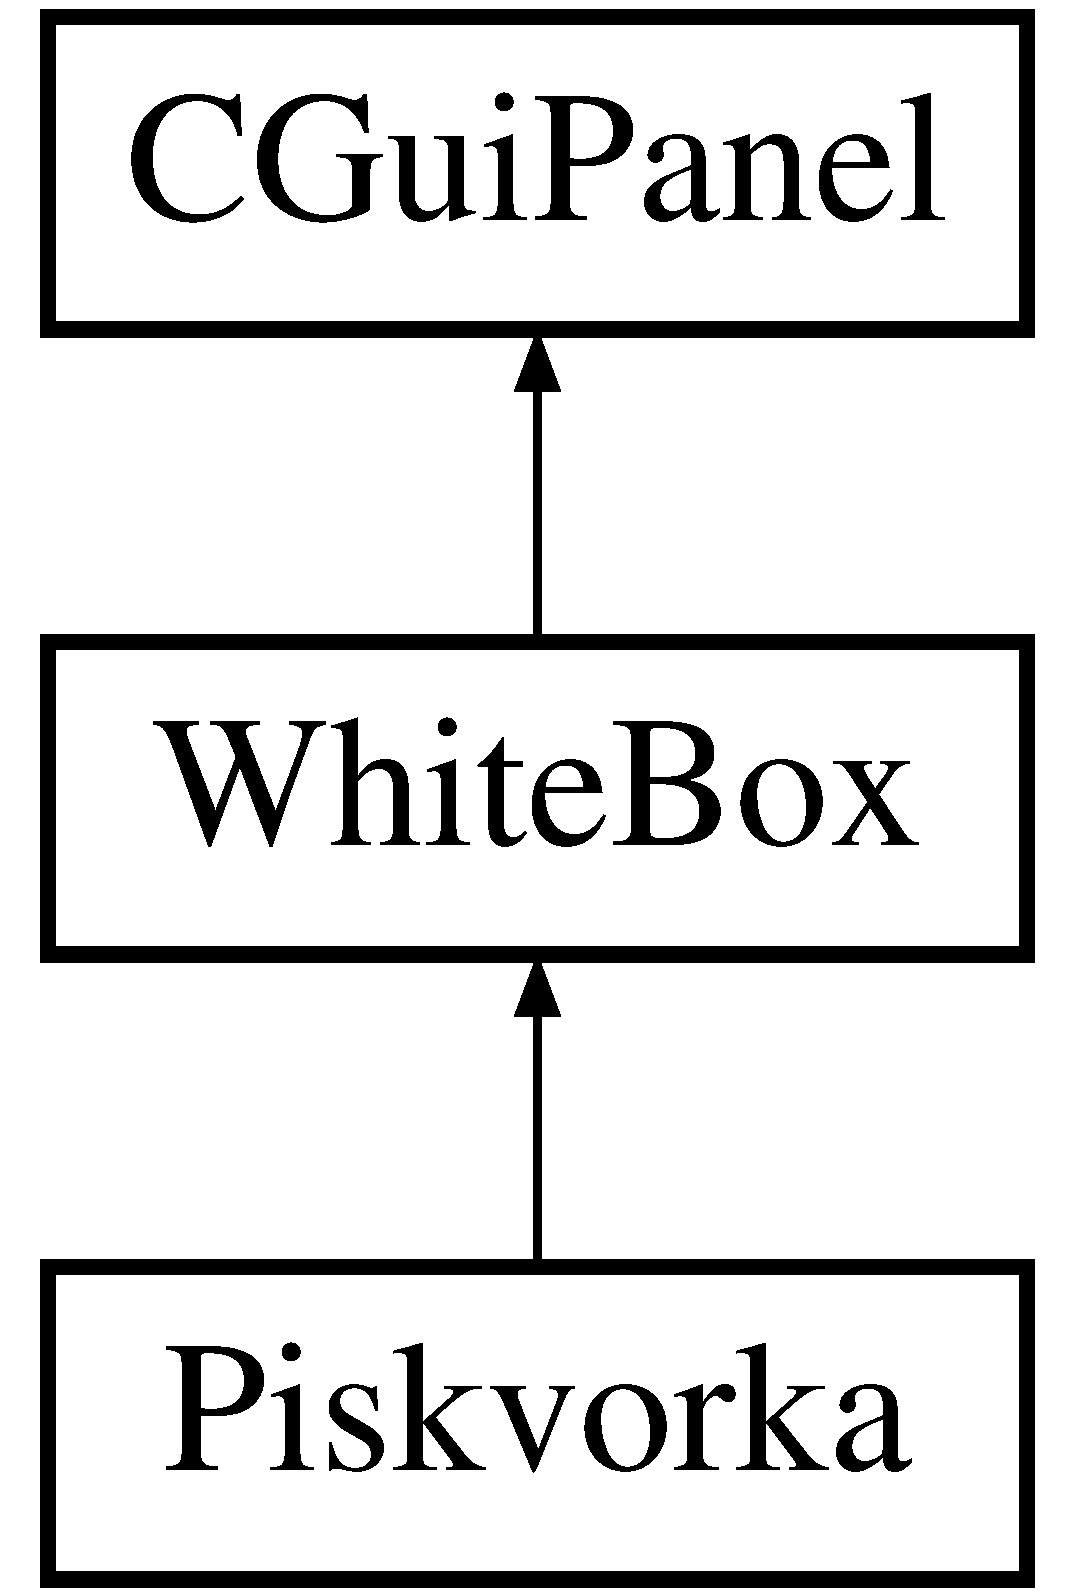
\includegraphics[height=3.000000cm]{class_piskvorka}
\end{center}
\end{figure}
\subsection*{Public Member Functions}
\begin{DoxyCompactItemize}
\item 
\hypertarget{class_piskvorka_a8d94b3b903f21a86bf029bd18b48e931}{
{\bfseries Piskvorka} (double x, double y, double w, double h)}
\label{class_piskvorka_a8d94b3b903f21a86bf029bd18b48e931}

\item 
\hypertarget{class_piskvorka_af19ec1df30afb349668b2834034f0fe9}{
bool {\bfseries onClick} (const \hyperlink{classvec2d}{vec2d} \&position, MouseButton button)}
\label{class_piskvorka_af19ec1df30afb349668b2834034f0fe9}

\end{DoxyCompactItemize}
\subsection*{Public Attributes}
\begin{DoxyCompactItemize}
\item 
\hypertarget{class_piskvorka_a9f41bd03cf8e1f1be6f86375506a56d0}{
bool {\bfseries isSet}}
\label{class_piskvorka_a9f41bd03cf8e1f1be6f86375506a56d0}

\end{DoxyCompactItemize}


The documentation for this class was generated from the following files:\begin{DoxyCompactItemize}
\item 
src/Piskvorka.h\item 
src/Piskvorka.cpp\end{DoxyCompactItemize}

\hypertarget{struct_p_s___blend_rec__}{
\section{PS\_\-BlendRec\_\- Struct Reference}
\label{struct_p_s___blend_rec__}\index{PS\_\-BlendRec\_\-@{PS\_\-BlendRec\_\-}}
}
\subsection*{Public Attributes}
\begin{DoxyCompactItemize}
\item 
\hypertarget{struct_p_s___blend_rec___ad81cbf3697f89908e9c15071e2ab9cac}{
FT\_\-UInt {\bfseries num\_\-designs}}
\label{struct_p_s___blend_rec___ad81cbf3697f89908e9c15071e2ab9cac}

\item 
\hypertarget{struct_p_s___blend_rec___af9b375493ee2d450cabbc571473e4006}{
FT\_\-UInt {\bfseries num\_\-axis}}
\label{struct_p_s___blend_rec___af9b375493ee2d450cabbc571473e4006}

\item 
\hypertarget{struct_p_s___blend_rec___afc0e4018ff3439f306d61e3c219b91f9}{
FT\_\-String $\ast$ {\bfseries axis\_\-names} \mbox{[}T1\_\-MAX\_\-MM\_\-AXIS\mbox{]}}
\label{struct_p_s___blend_rec___afc0e4018ff3439f306d61e3c219b91f9}

\item 
\hypertarget{struct_p_s___blend_rec___ad0e6c9b9d42346fd8a3371a5b2473e3c}{
FT\_\-Fixed $\ast$ {\bfseries design\_\-pos} \mbox{[}T1\_\-MAX\_\-MM\_\-DESIGNS\mbox{]}}
\label{struct_p_s___blend_rec___ad0e6c9b9d42346fd8a3371a5b2473e3c}

\item 
\hypertarget{struct_p_s___blend_rec___a005c783c65e5dd35611e88901b5db2ca}{
\hyperlink{struct_p_s___design_map__}{PS\_\-DesignMapRec} {\bfseries design\_\-map} \mbox{[}T1\_\-MAX\_\-MM\_\-AXIS\mbox{]}}
\label{struct_p_s___blend_rec___a005c783c65e5dd35611e88901b5db2ca}

\item 
\hypertarget{struct_p_s___blend_rec___ae3dcbb2aaee676fdc3d5bde890b2cc78}{
FT\_\-Fixed $\ast$ {\bfseries weight\_\-vector}}
\label{struct_p_s___blend_rec___ae3dcbb2aaee676fdc3d5bde890b2cc78}

\item 
\hypertarget{struct_p_s___blend_rec___a29c19d988e8ee1eb4f333b1ac55759de}{
FT\_\-Fixed $\ast$ {\bfseries default\_\-weight\_\-vector}}
\label{struct_p_s___blend_rec___a29c19d988e8ee1eb4f333b1ac55759de}

\item 
\hypertarget{struct_p_s___blend_rec___ac5478cafc838257e693a9604edf1f5e9}{
\hyperlink{struct_p_s___font_info_rec__}{PS\_\-FontInfo} {\bfseries font\_\-infos} \mbox{[}T1\_\-MAX\_\-MM\_\-DESIGNS+1\mbox{]}}
\label{struct_p_s___blend_rec___ac5478cafc838257e693a9604edf1f5e9}

\item 
\hypertarget{struct_p_s___blend_rec___a2b6e0c48d7a9c350b09f2943c1779ea4}{
\hyperlink{struct_p_s___private_rec__}{PS\_\-Private} {\bfseries privates} \mbox{[}T1\_\-MAX\_\-MM\_\-DESIGNS+1\mbox{]}}
\label{struct_p_s___blend_rec___a2b6e0c48d7a9c350b09f2943c1779ea4}

\item 
\hypertarget{struct_p_s___blend_rec___a86caa5319e208b4a2057db656bad9221}{
FT\_\-ULong {\bfseries blend\_\-bitflags}}
\label{struct_p_s___blend_rec___a86caa5319e208b4a2057db656bad9221}

\item 
\hypertarget{struct_p_s___blend_rec___a30845d3cbd2e95a5f9cc867c7226af5e}{
\hyperlink{struct_f_t___b_box__}{FT\_\-BBox} $\ast$ {\bfseries bboxes} \mbox{[}T1\_\-MAX\_\-MM\_\-DESIGNS+1\mbox{]}}
\label{struct_p_s___blend_rec___a30845d3cbd2e95a5f9cc867c7226af5e}

\item 
\hypertarget{struct_p_s___blend_rec___a3ddacbda91fe0f9ef934a9e0afa6286f}{
FT\_\-UInt {\bfseries default\_\-design\_\-vector} \mbox{[}T1\_\-MAX\_\-MM\_\-DESIGNS\mbox{]}}
\label{struct_p_s___blend_rec___a3ddacbda91fe0f9ef934a9e0afa6286f}

\item 
\hypertarget{struct_p_s___blend_rec___afa5c7dd4206eb8a1d9ef4894abfc9555}{
FT\_\-UInt {\bfseries num\_\-default\_\-design\_\-vector}}
\label{struct_p_s___blend_rec___afa5c7dd4206eb8a1d9ef4894abfc9555}

\end{DoxyCompactItemize}


The documentation for this struct was generated from the following file:\begin{DoxyCompactItemize}
\item 
src/libs/freetype/t1tables.h\end{DoxyCompactItemize}

\hypertarget{struct_p_s___design_map__}{
\section{PS\_\-DesignMap\_\- Struct Reference}
\label{struct_p_s___design_map__}\index{PS\_\-DesignMap\_\-@{PS\_\-DesignMap\_\-}}
}
\subsection*{Public Attributes}
\begin{DoxyCompactItemize}
\item 
\hypertarget{struct_p_s___design_map___a505a70dd0f497f177fffca9bc4e5d0a5}{
FT\_\-Byte {\bfseries num\_\-points}}
\label{struct_p_s___design_map___a505a70dd0f497f177fffca9bc4e5d0a5}

\item 
\hypertarget{struct_p_s___design_map___abd7a86ba33248ceed657c31063b49679}{
FT\_\-Long $\ast$ {\bfseries design\_\-points}}
\label{struct_p_s___design_map___abd7a86ba33248ceed657c31063b49679}

\item 
\hypertarget{struct_p_s___design_map___a74a555fb4315fca7477f6d20d49686ec}{
FT\_\-Fixed $\ast$ {\bfseries blend\_\-points}}
\label{struct_p_s___design_map___a74a555fb4315fca7477f6d20d49686ec}

\end{DoxyCompactItemize}


The documentation for this struct was generated from the following file:\begin{DoxyCompactItemize}
\item 
src/libs/freetype/t1tables.h\end{DoxyCompactItemize}

\hypertarget{struct_p_s___font_extra_rec__}{
\section{PS\_\-FontExtraRec\_\- Struct Reference}
\label{struct_p_s___font_extra_rec__}\index{PS\_\-FontExtraRec\_\-@{PS\_\-FontExtraRec\_\-}}
}
\subsection*{Public Attributes}
\begin{DoxyCompactItemize}
\item 
\hypertarget{struct_p_s___font_extra_rec___a048e1e57ee974c3e05e9a88476e6b8a9}{
FT\_\-UShort {\bfseries fs\_\-type}}
\label{struct_p_s___font_extra_rec___a048e1e57ee974c3e05e9a88476e6b8a9}

\end{DoxyCompactItemize}


The documentation for this struct was generated from the following file:\begin{DoxyCompactItemize}
\item 
src/libs/freetype/internal/t1types.h\end{DoxyCompactItemize}

\hypertarget{struct_p_s___font_info_rec__}{
\section{PS\_\-FontInfoRec\_\- Struct Reference}
\label{struct_p_s___font_info_rec__}\index{PS\_\-FontInfoRec\_\-@{PS\_\-FontInfoRec\_\-}}
}
\subsection*{Public Attributes}
\begin{DoxyCompactItemize}
\item 
\hypertarget{struct_p_s___font_info_rec___adb595076e50f8e7ece9446f612433cfc}{
FT\_\-String $\ast$ {\bfseries version}}
\label{struct_p_s___font_info_rec___adb595076e50f8e7ece9446f612433cfc}

\item 
\hypertarget{struct_p_s___font_info_rec___a63858ebce653f21d9aa2ddc61ee32b80}{
FT\_\-String $\ast$ {\bfseries notice}}
\label{struct_p_s___font_info_rec___a63858ebce653f21d9aa2ddc61ee32b80}

\item 
\hypertarget{struct_p_s___font_info_rec___a039dbf76ccc1b63b03e77215cb4b430b}{
FT\_\-String $\ast$ {\bfseries full\_\-name}}
\label{struct_p_s___font_info_rec___a039dbf76ccc1b63b03e77215cb4b430b}

\item 
\hypertarget{struct_p_s___font_info_rec___ac54d883f153a495f9a20dc043ed434cf}{
FT\_\-String $\ast$ {\bfseries family\_\-name}}
\label{struct_p_s___font_info_rec___ac54d883f153a495f9a20dc043ed434cf}

\item 
\hypertarget{struct_p_s___font_info_rec___a057243ec7cf62f573fa675ccb728f4b1}{
FT\_\-String $\ast$ {\bfseries weight}}
\label{struct_p_s___font_info_rec___a057243ec7cf62f573fa675ccb728f4b1}

\item 
\hypertarget{struct_p_s___font_info_rec___ab558a75a56fadd54dfc71dcbeec1375a}{
FT\_\-Long {\bfseries italic\_\-angle}}
\label{struct_p_s___font_info_rec___ab558a75a56fadd54dfc71dcbeec1375a}

\item 
\hypertarget{struct_p_s___font_info_rec___a68e2d0913fe910ea86d558a4a426412a}{
FT\_\-Bool {\bfseries is\_\-fixed\_\-pitch}}
\label{struct_p_s___font_info_rec___a68e2d0913fe910ea86d558a4a426412a}

\item 
\hypertarget{struct_p_s___font_info_rec___a772af52d17288d7846e8893e74d55212}{
FT\_\-Short {\bfseries underline\_\-position}}
\label{struct_p_s___font_info_rec___a772af52d17288d7846e8893e74d55212}

\item 
\hypertarget{struct_p_s___font_info_rec___a423904e811db5195485557bf0dccf126}{
FT\_\-UShort {\bfseries underline\_\-thickness}}
\label{struct_p_s___font_info_rec___a423904e811db5195485557bf0dccf126}

\end{DoxyCompactItemize}


The documentation for this struct was generated from the following file:\begin{DoxyCompactItemize}
\item 
src/libs/freetype/t1tables.h\end{DoxyCompactItemize}

\hypertarget{struct_p_s___parser___funcs_rec__}{
\section{PS\_\-Parser\_\-FuncsRec\_\- Struct Reference}
\label{struct_p_s___parser___funcs_rec__}\index{PS\_\-Parser\_\-FuncsRec\_\-@{PS\_\-Parser\_\-FuncsRec\_\-}}
}
\subsection*{Public Attributes}
\begin{DoxyCompactItemize}
\item 
\hypertarget{struct_p_s___parser___funcs_rec___ab85cca9562d53b5ee3142e0f5c1b8a9b}{
void($\ast$ {\bfseries init} )(\hyperlink{struct_p_s___parser_rec__}{PS\_\-Parser} parser, FT\_\-Byte $\ast$base, FT\_\-Byte $\ast$limit, FT\_\-Memory memory)}
\label{struct_p_s___parser___funcs_rec___ab85cca9562d53b5ee3142e0f5c1b8a9b}

\item 
\hypertarget{struct_p_s___parser___funcs_rec___a9351f4dfa31c817d74c1a65741a71c8d}{
void($\ast$ {\bfseries done} )(\hyperlink{struct_p_s___parser_rec__}{PS\_\-Parser} parser)}
\label{struct_p_s___parser___funcs_rec___a9351f4dfa31c817d74c1a65741a71c8d}

\item 
\hypertarget{struct_p_s___parser___funcs_rec___a3ebff5e8cf80ee2051858bc456c2f388}{
void($\ast$ {\bfseries skip\_\-spaces} )(\hyperlink{struct_p_s___parser_rec__}{PS\_\-Parser} parser)}
\label{struct_p_s___parser___funcs_rec___a3ebff5e8cf80ee2051858bc456c2f388}

\item 
\hypertarget{struct_p_s___parser___funcs_rec___a786db660e0ba4418b2e60e2b91c3f1e9}{
void($\ast$ {\bfseries skip\_\-PS\_\-token} )(\hyperlink{struct_p_s___parser_rec__}{PS\_\-Parser} parser)}
\label{struct_p_s___parser___funcs_rec___a786db660e0ba4418b2e60e2b91c3f1e9}

\item 
\hypertarget{struct_p_s___parser___funcs_rec___a59a2017715d1a0db810c6e38ad3a4a67}{
FT\_\-Long($\ast$ {\bfseries to\_\-int} )(\hyperlink{struct_p_s___parser_rec__}{PS\_\-Parser} parser)}
\label{struct_p_s___parser___funcs_rec___a59a2017715d1a0db810c6e38ad3a4a67}

\item 
\hypertarget{struct_p_s___parser___funcs_rec___a7a67e9c9b8fc0e0aedb37476f107e835}{
FT\_\-Fixed($\ast$ {\bfseries to\_\-fixed} )(\hyperlink{struct_p_s___parser_rec__}{PS\_\-Parser} parser, FT\_\-Int power\_\-ten)}
\label{struct_p_s___parser___funcs_rec___a7a67e9c9b8fc0e0aedb37476f107e835}

\item 
\hypertarget{struct_p_s___parser___funcs_rec___abbda6afe648361ec1efa535fc853ce54}{
FT\_\-Error($\ast$ {\bfseries to\_\-bytes} )(\hyperlink{struct_p_s___parser_rec__}{PS\_\-Parser} parser, FT\_\-Byte $\ast$bytes, FT\_\-Offset max\_\-bytes, FT\_\-Long $\ast$pnum\_\-bytes, FT\_\-Bool delimiters)}
\label{struct_p_s___parser___funcs_rec___abbda6afe648361ec1efa535fc853ce54}

\item 
\hypertarget{struct_p_s___parser___funcs_rec___a11da5ac33187bc7b67696a9d24f3d239}{
FT\_\-Int($\ast$ {\bfseries to\_\-coord\_\-array} )(\hyperlink{struct_p_s___parser_rec__}{PS\_\-Parser} parser, FT\_\-Int max\_\-coords, FT\_\-Short $\ast$coords)}
\label{struct_p_s___parser___funcs_rec___a11da5ac33187bc7b67696a9d24f3d239}

\item 
\hypertarget{struct_p_s___parser___funcs_rec___a5b9316c7a5459857da99f6158afdf3d9}{
FT\_\-Int($\ast$ {\bfseries to\_\-fixed\_\-array} )(\hyperlink{struct_p_s___parser_rec__}{PS\_\-Parser} parser, FT\_\-Int max\_\-values, FT\_\-Fixed $\ast$values, FT\_\-Int power\_\-ten)}
\label{struct_p_s___parser___funcs_rec___a5b9316c7a5459857da99f6158afdf3d9}

\item 
\hypertarget{struct_p_s___parser___funcs_rec___ad963b97fac4a1ae52f4a68e693f39907}{
void($\ast$ {\bfseries to\_\-token} )(\hyperlink{struct_p_s___parser_rec__}{PS\_\-Parser} parser, \hyperlink{struct_t1___token_rec__}{T1\_\-Token} token)}
\label{struct_p_s___parser___funcs_rec___ad963b97fac4a1ae52f4a68e693f39907}

\item 
\hypertarget{struct_p_s___parser___funcs_rec___ac3cb6fd9c5eb16d8d853fa02e57602c2}{
void($\ast$ {\bfseries to\_\-token\_\-array} )(\hyperlink{struct_p_s___parser_rec__}{PS\_\-Parser} parser, \hyperlink{struct_t1___token_rec__}{T1\_\-Token} tokens, FT\_\-UInt max\_\-tokens, FT\_\-Int $\ast$pnum\_\-tokens)}
\label{struct_p_s___parser___funcs_rec___ac3cb6fd9c5eb16d8d853fa02e57602c2}

\item 
\hypertarget{struct_p_s___parser___funcs_rec___a1e3a763197f876746bc053bee27a3b86}{
FT\_\-Error($\ast$ {\bfseries load\_\-field} )(\hyperlink{struct_p_s___parser_rec__}{PS\_\-Parser} parser, const \hyperlink{struct_t1___field_rec__}{T1\_\-Field} field, void $\ast$$\ast$objects, FT\_\-UInt max\_\-objects, FT\_\-ULong $\ast$pflags)}
\label{struct_p_s___parser___funcs_rec___a1e3a763197f876746bc053bee27a3b86}

\item 
\hypertarget{struct_p_s___parser___funcs_rec___ac925f8b8b583c22717da0475a2427863}{
FT\_\-Error($\ast$ {\bfseries load\_\-field\_\-table} )(\hyperlink{struct_p_s___parser_rec__}{PS\_\-Parser} parser, const \hyperlink{struct_t1___field_rec__}{T1\_\-Field} field, void $\ast$$\ast$objects, FT\_\-UInt max\_\-objects, FT\_\-ULong $\ast$pflags)}
\label{struct_p_s___parser___funcs_rec___ac925f8b8b583c22717da0475a2427863}

\end{DoxyCompactItemize}


The documentation for this struct was generated from the following file:\begin{DoxyCompactItemize}
\item 
src/libs/freetype/internal/psaux.h\end{DoxyCompactItemize}

\hypertarget{struct_p_s___parser_rec__}{
\section{PS\_\-ParserRec\_\- Struct Reference}
\label{struct_p_s___parser_rec__}\index{PS\_\-ParserRec\_\-@{PS\_\-ParserRec\_\-}}
}
\subsection*{Public Attributes}
\begin{DoxyCompactItemize}
\item 
\hypertarget{struct_p_s___parser_rec___a6ed189bc25c03814bdafad63819ddfe7}{
FT\_\-Byte $\ast$ {\bfseries cursor}}
\label{struct_p_s___parser_rec___a6ed189bc25c03814bdafad63819ddfe7}

\item 
\hypertarget{struct_p_s___parser_rec___a30528f6a9caffce2fd44ef2d5a38e5bd}{
FT\_\-Byte $\ast$ {\bfseries base}}
\label{struct_p_s___parser_rec___a30528f6a9caffce2fd44ef2d5a38e5bd}

\item 
\hypertarget{struct_p_s___parser_rec___af3310795fd73530036fb32ec4385ea3d}{
FT\_\-Byte $\ast$ {\bfseries limit}}
\label{struct_p_s___parser_rec___af3310795fd73530036fb32ec4385ea3d}

\item 
\hypertarget{struct_p_s___parser_rec___a7a1432cb4d8bb603663f1258224c8ec4}{
FT\_\-Error {\bfseries error}}
\label{struct_p_s___parser_rec___a7a1432cb4d8bb603663f1258224c8ec4}

\item 
\hypertarget{struct_p_s___parser_rec___a3e2206deb6c0d73f51c8c71d5db1db1f}{
FT\_\-Memory {\bfseries memory}}
\label{struct_p_s___parser_rec___a3e2206deb6c0d73f51c8c71d5db1db1f}

\item 
\hypertarget{struct_p_s___parser_rec___a450031fd9e77e55bf424dc64a8d2659d}{
\hyperlink{struct_p_s___parser___funcs_rec__}{PS\_\-Parser\_\-FuncsRec} {\bfseries funcs}}
\label{struct_p_s___parser_rec___a450031fd9e77e55bf424dc64a8d2659d}

\end{DoxyCompactItemize}


The documentation for this struct was generated from the following file:\begin{DoxyCompactItemize}
\item 
src/libs/freetype/internal/psaux.h\end{DoxyCompactItemize}

\hypertarget{struct_p_s___private_rec__}{
\section{PS\_\-PrivateRec\_\- Struct Reference}
\label{struct_p_s___private_rec__}\index{PS\_\-PrivateRec\_\-@{PS\_\-PrivateRec\_\-}}
}
\subsection*{Public Attributes}
\begin{DoxyCompactItemize}
\item 
\hypertarget{struct_p_s___private_rec___ae862c1db170cfee85aa3242be9fa5d57}{
FT\_\-Int {\bfseries unique\_\-id}}
\label{struct_p_s___private_rec___ae862c1db170cfee85aa3242be9fa5d57}

\item 
\hypertarget{struct_p_s___private_rec___a796ebb92d96f0297ae584a911768db8b}{
FT\_\-Int {\bfseries lenIV}}
\label{struct_p_s___private_rec___a796ebb92d96f0297ae584a911768db8b}

\item 
\hypertarget{struct_p_s___private_rec___ae3c56e75b5674451a7296cbb9f0a2e40}{
FT\_\-Byte {\bfseries num\_\-blue\_\-values}}
\label{struct_p_s___private_rec___ae3c56e75b5674451a7296cbb9f0a2e40}

\item 
\hypertarget{struct_p_s___private_rec___a149acdf871b0739f7ab13b1ac8e48a28}{
FT\_\-Byte {\bfseries num\_\-other\_\-blues}}
\label{struct_p_s___private_rec___a149acdf871b0739f7ab13b1ac8e48a28}

\item 
\hypertarget{struct_p_s___private_rec___a1e8a432c78f00034c73cfc54c787b10f}{
FT\_\-Byte {\bfseries num\_\-family\_\-blues}}
\label{struct_p_s___private_rec___a1e8a432c78f00034c73cfc54c787b10f}

\item 
\hypertarget{struct_p_s___private_rec___a7370e2e89f39f7ff8923f3d1befbcfce}{
FT\_\-Byte {\bfseries num\_\-family\_\-other\_\-blues}}
\label{struct_p_s___private_rec___a7370e2e89f39f7ff8923f3d1befbcfce}

\item 
\hypertarget{struct_p_s___private_rec___ae2c23ed06e54b680473f924483685425}{
FT\_\-Short {\bfseries blue\_\-values} \mbox{[}14\mbox{]}}
\label{struct_p_s___private_rec___ae2c23ed06e54b680473f924483685425}

\item 
\hypertarget{struct_p_s___private_rec___a6da97f89e174d621936c75fe9b463e65}{
FT\_\-Short {\bfseries other\_\-blues} \mbox{[}10\mbox{]}}
\label{struct_p_s___private_rec___a6da97f89e174d621936c75fe9b463e65}

\item 
\hypertarget{struct_p_s___private_rec___aa6645b5810e4e8b7d1a8b57300cdf406}{
FT\_\-Short {\bfseries family\_\-blues} \mbox{[}14\mbox{]}}
\label{struct_p_s___private_rec___aa6645b5810e4e8b7d1a8b57300cdf406}

\item 
\hypertarget{struct_p_s___private_rec___aaff4f071eee676aff4e5ca61ba30c218}{
FT\_\-Short {\bfseries family\_\-other\_\-blues} \mbox{[}10\mbox{]}}
\label{struct_p_s___private_rec___aaff4f071eee676aff4e5ca61ba30c218}

\item 
\hypertarget{struct_p_s___private_rec___aef435ab2e5ad52aa4e2ad3eed14b6666}{
FT\_\-Fixed {\bfseries blue\_\-scale}}
\label{struct_p_s___private_rec___aef435ab2e5ad52aa4e2ad3eed14b6666}

\item 
\hypertarget{struct_p_s___private_rec___aaf1a9f747580eb6618422e3c5b77ae82}{
FT\_\-Int {\bfseries blue\_\-shift}}
\label{struct_p_s___private_rec___aaf1a9f747580eb6618422e3c5b77ae82}

\item 
\hypertarget{struct_p_s___private_rec___a21fbb2665f25cd0d769d023ca8063319}{
FT\_\-Int {\bfseries blue\_\-fuzz}}
\label{struct_p_s___private_rec___a21fbb2665f25cd0d769d023ca8063319}

\item 
\hypertarget{struct_p_s___private_rec___a1c8ae2204e63c22b7702446720ed50a3}{
FT\_\-UShort {\bfseries standard\_\-width} \mbox{[}1\mbox{]}}
\label{struct_p_s___private_rec___a1c8ae2204e63c22b7702446720ed50a3}

\item 
\hypertarget{struct_p_s___private_rec___a89aed70a7b26aafe320e7733eaeb400e}{
FT\_\-UShort {\bfseries standard\_\-height} \mbox{[}1\mbox{]}}
\label{struct_p_s___private_rec___a89aed70a7b26aafe320e7733eaeb400e}

\item 
\hypertarget{struct_p_s___private_rec___a0bd8b3c1b86b2b3ff66e44cba5297d07}{
FT\_\-Byte {\bfseries num\_\-snap\_\-widths}}
\label{struct_p_s___private_rec___a0bd8b3c1b86b2b3ff66e44cba5297d07}

\item 
\hypertarget{struct_p_s___private_rec___a53f7cfd204400a00eb7203b67d6a1b1c}{
FT\_\-Byte {\bfseries num\_\-snap\_\-heights}}
\label{struct_p_s___private_rec___a53f7cfd204400a00eb7203b67d6a1b1c}

\item 
\hypertarget{struct_p_s___private_rec___a40e62a278e48f47a0f204bd9fa5c883f}{
FT\_\-Bool {\bfseries force\_\-bold}}
\label{struct_p_s___private_rec___a40e62a278e48f47a0f204bd9fa5c883f}

\item 
\hypertarget{struct_p_s___private_rec___a96b9729811d02146a87ffdc5c254bbe9}{
FT\_\-Bool {\bfseries round\_\-stem\_\-up}}
\label{struct_p_s___private_rec___a96b9729811d02146a87ffdc5c254bbe9}

\item 
\hypertarget{struct_p_s___private_rec___a39cf1a4b21280bf8082ccba0f4824a8a}{
FT\_\-Short {\bfseries snap\_\-widths} \mbox{[}13\mbox{]}}
\label{struct_p_s___private_rec___a39cf1a4b21280bf8082ccba0f4824a8a}

\item 
\hypertarget{struct_p_s___private_rec___a3583caf0cc05de2afac098574ed0bc4b}{
FT\_\-Short {\bfseries snap\_\-heights} \mbox{[}13\mbox{]}}
\label{struct_p_s___private_rec___a3583caf0cc05de2afac098574ed0bc4b}

\item 
\hypertarget{struct_p_s___private_rec___a45cf6e07c4c26f029e66998e6cad9fa0}{
FT\_\-Fixed {\bfseries expansion\_\-factor}}
\label{struct_p_s___private_rec___a45cf6e07c4c26f029e66998e6cad9fa0}

\item 
\hypertarget{struct_p_s___private_rec___afc2a7f950a174577ebfc062bb1598f5c}{
FT\_\-Long {\bfseries language\_\-group}}
\label{struct_p_s___private_rec___afc2a7f950a174577ebfc062bb1598f5c}

\item 
\hypertarget{struct_p_s___private_rec___a309a871cdeb6f658d8fbff23fa13b667}{
FT\_\-Long {\bfseries password}}
\label{struct_p_s___private_rec___a309a871cdeb6f658d8fbff23fa13b667}

\item 
\hypertarget{struct_p_s___private_rec___af8c829e03c424b1f12b2c9cd4041a868}{
FT\_\-Short {\bfseries min\_\-feature} \mbox{[}2\mbox{]}}
\label{struct_p_s___private_rec___af8c829e03c424b1f12b2c9cd4041a868}

\end{DoxyCompactItemize}


The documentation for this struct was generated from the following file:\begin{DoxyCompactItemize}
\item 
src/libs/freetype/t1tables.h\end{DoxyCompactItemize}

\hypertarget{struct_p_s___table___funcs_rec__}{
\section{PS\_\-Table\_\-FuncsRec\_\- Struct Reference}
\label{struct_p_s___table___funcs_rec__}\index{PS\_\-Table\_\-FuncsRec\_\-@{PS\_\-Table\_\-FuncsRec\_\-}}
}
\subsection*{Public Attributes}
\begin{DoxyCompactItemize}
\item 
\hypertarget{struct_p_s___table___funcs_rec___ad0e795ae1e8a7040b7ef80d4a46e8d6a}{
FT\_\-Error($\ast$ {\bfseries init} )(PS\_\-Table table, FT\_\-Int count, FT\_\-Memory memory)}
\label{struct_p_s___table___funcs_rec___ad0e795ae1e8a7040b7ef80d4a46e8d6a}

\item 
\hypertarget{struct_p_s___table___funcs_rec___a33d660e1444fbe0ef35a87645f5831ad}{
void($\ast$ {\bfseries done} )(PS\_\-Table table)}
\label{struct_p_s___table___funcs_rec___a33d660e1444fbe0ef35a87645f5831ad}

\item 
\hypertarget{struct_p_s___table___funcs_rec___a38a0e111e48a877f52cce490362e4c91}{
FT\_\-Error($\ast$ {\bfseries add} )(PS\_\-Table table, FT\_\-Int idx, void $\ast$object, FT\_\-PtrDist length)}
\label{struct_p_s___table___funcs_rec___a38a0e111e48a877f52cce490362e4c91}

\item 
\hypertarget{struct_p_s___table___funcs_rec___a252959418225279f78e2ece7fc7705bd}{
void($\ast$ {\bfseries release} )(PS\_\-Table table)}
\label{struct_p_s___table___funcs_rec___a252959418225279f78e2ece7fc7705bd}

\end{DoxyCompactItemize}


The documentation for this struct was generated from the following file:\begin{DoxyCompactItemize}
\item 
src/libs/freetype/internal/psaux.h\end{DoxyCompactItemize}

\hypertarget{struct_p_s___table_rec__}{
\section{PS\_\-TableRec\_\- Struct Reference}
\label{struct_p_s___table_rec__}\index{PS\_\-TableRec\_\-@{PS\_\-TableRec\_\-}}
}
\subsection*{Public Attributes}
\begin{DoxyCompactItemize}
\item 
\hypertarget{struct_p_s___table_rec___a6caa7b6aef2ba7e28d260b6a87782723}{
FT\_\-Byte $\ast$ {\bfseries block}}
\label{struct_p_s___table_rec___a6caa7b6aef2ba7e28d260b6a87782723}

\item 
\hypertarget{struct_p_s___table_rec___a8725d30f75b6dc785b988ed689ac7e58}{
FT\_\-Offset {\bfseries cursor}}
\label{struct_p_s___table_rec___a8725d30f75b6dc785b988ed689ac7e58}

\item 
\hypertarget{struct_p_s___table_rec___acf6d4f15ca247960cc7823b73d3c66bf}{
FT\_\-Offset {\bfseries capacity}}
\label{struct_p_s___table_rec___acf6d4f15ca247960cc7823b73d3c66bf}

\item 
\hypertarget{struct_p_s___table_rec___aa76fb2bcdcf4fc75e880b092bb9d3115}{
FT\_\-Long {\bfseries init}}
\label{struct_p_s___table_rec___aa76fb2bcdcf4fc75e880b092bb9d3115}

\item 
\hypertarget{struct_p_s___table_rec___a8594ec199ad792ed7ffd558806a7d23b}{
FT\_\-Int {\bfseries max\_\-elems}}
\label{struct_p_s___table_rec___a8594ec199ad792ed7ffd558806a7d23b}

\item 
\hypertarget{struct_p_s___table_rec___a26706016251497b19039f2c002c4e9d5}{
FT\_\-Int {\bfseries num\_\-elems}}
\label{struct_p_s___table_rec___a26706016251497b19039f2c002c4e9d5}

\item 
\hypertarget{struct_p_s___table_rec___a1967f81d98ea65a605968a7e1e5c51c3}{
FT\_\-Byte $\ast$$\ast$ {\bfseries elements}}
\label{struct_p_s___table_rec___a1967f81d98ea65a605968a7e1e5c51c3}

\item 
\hypertarget{struct_p_s___table_rec___a955ae6315b89923f1074f3d046da23b1}{
FT\_\-PtrDist $\ast$ {\bfseries lengths}}
\label{struct_p_s___table_rec___a955ae6315b89923f1074f3d046da23b1}

\item 
\hypertarget{struct_p_s___table_rec___a061872add9c6d1af67cfdfac5ce2b80d}{
FT\_\-Memory {\bfseries memory}}
\label{struct_p_s___table_rec___a061872add9c6d1af67cfdfac5ce2b80d}

\item 
\hypertarget{struct_p_s___table_rec___adced5ad36107c90012e9fafa55eab5b9}{
\hyperlink{struct_p_s___table___funcs_rec__}{PS\_\-Table\_\-FuncsRec} {\bfseries funcs}}
\label{struct_p_s___table_rec___adced5ad36107c90012e9fafa55eab5b9}

\end{DoxyCompactItemize}


The documentation for this struct was generated from the following file:\begin{DoxyCompactItemize}
\item 
src/libs/freetype/internal/psaux.h\end{DoxyCompactItemize}

\hypertarget{struct_p_s___unicodes_rec__}{
\section{PS\_\-UnicodesRec\_\- Struct Reference}
\label{struct_p_s___unicodes_rec__}\index{PS\_\-UnicodesRec\_\-@{PS\_\-UnicodesRec\_\-}}
}
\subsection*{Public Attributes}
\begin{DoxyCompactItemize}
\item 
\hypertarget{struct_p_s___unicodes_rec___a4c3e28cb86c8a7039107437dcf995da7}{
\hyperlink{struct_f_t___c_map_rec__}{FT\_\-CMapRec} {\bfseries cmap}}
\label{struct_p_s___unicodes_rec___a4c3e28cb86c8a7039107437dcf995da7}

\item 
\hypertarget{struct_p_s___unicodes_rec___abbc3617f13363ddcf851ee229752b08d}{
FT\_\-UInt {\bfseries num\_\-maps}}
\label{struct_p_s___unicodes_rec___abbc3617f13363ddcf851ee229752b08d}

\item 
\hypertarget{struct_p_s___unicodes_rec___abd0ff1abe19a2a6a838b631ec81d22cd}{
\hyperlink{struct_p_s___uni_map__}{PS\_\-UniMap} $\ast$ {\bfseries maps}}
\label{struct_p_s___unicodes_rec___abd0ff1abe19a2a6a838b631ec81d22cd}

\end{DoxyCompactItemize}


The documentation for this struct was generated from the following file:\begin{DoxyCompactItemize}
\item 
src/libs/freetype/internal/services/svpscmap.h\end{DoxyCompactItemize}

\hypertarget{struct_p_s___uni_map__}{
\section{PS\_\-UniMap\_\- Struct Reference}
\label{struct_p_s___uni_map__}\index{PS\_\-UniMap\_\-@{PS\_\-UniMap\_\-}}
}
\subsection*{Public Attributes}
\begin{DoxyCompactItemize}
\item 
\hypertarget{struct_p_s___uni_map___a87c1f471eb4033fc5ed9d0f1ecaf35a1}{
FT\_\-UInt32 {\bfseries unicode}}
\label{struct_p_s___uni_map___a87c1f471eb4033fc5ed9d0f1ecaf35a1}

\item 
\hypertarget{struct_p_s___uni_map___a0d5b2e3c405aeab1f1059a3587125cfd}{
FT\_\-UInt {\bfseries glyph\_\-index}}
\label{struct_p_s___uni_map___a0d5b2e3c405aeab1f1059a3587125cfd}

\end{DoxyCompactItemize}


The documentation for this struct was generated from the following file:\begin{DoxyCompactItemize}
\item 
src/libs/freetype/internal/services/svpscmap.h\end{DoxyCompactItemize}

\hypertarget{struct_p_s_aux___service_rec__}{
\section{PSAux\_\-ServiceRec\_\- Struct Reference}
\label{struct_p_s_aux___service_rec__}\index{PSAux\_\-ServiceRec\_\-@{PSAux\_\-ServiceRec\_\-}}
}
\subsection*{Public Attributes}
\begin{DoxyCompactItemize}
\item 
\hypertarget{struct_p_s_aux___service_rec___ad328bf7394cad5b2838822aa109acc42}{
const \hyperlink{struct_p_s___table___funcs_rec__}{PS\_\-Table\_\-FuncsRec} $\ast$ {\bfseries ps\_\-table\_\-funcs}}
\label{struct_p_s_aux___service_rec___ad328bf7394cad5b2838822aa109acc42}

\item 
\hypertarget{struct_p_s_aux___service_rec___ac673695e814332b38fd33c7f0287a4b7}{
const \hyperlink{struct_p_s___parser___funcs_rec__}{PS\_\-Parser\_\-FuncsRec} $\ast$ {\bfseries ps\_\-parser\_\-funcs}}
\label{struct_p_s_aux___service_rec___ac673695e814332b38fd33c7f0287a4b7}

\item 
\hypertarget{struct_p_s_aux___service_rec___a3fe7449b123d0fb6f7ba92462c4e94c1}{
const \hyperlink{struct_t1___builder___funcs_rec__}{T1\_\-Builder\_\-FuncsRec} $\ast$ {\bfseries t1\_\-builder\_\-funcs}}
\label{struct_p_s_aux___service_rec___a3fe7449b123d0fb6f7ba92462c4e94c1}

\item 
\hypertarget{struct_p_s_aux___service_rec___a5cfe03f55fa4c342a094fd31355835b2}{
const \hyperlink{struct_t1___decoder___funcs_rec__}{T1\_\-Decoder\_\-FuncsRec} $\ast$ {\bfseries t1\_\-decoder\_\-funcs}}
\label{struct_p_s_aux___service_rec___a5cfe03f55fa4c342a094fd31355835b2}

\item 
\hypertarget{struct_p_s_aux___service_rec___a908d3ea91a5c313015bc90568026d57c}{
void($\ast$ {\bfseries t1\_\-decrypt} )(FT\_\-Byte $\ast$buffer, FT\_\-Offset length, FT\_\-UShort seed)}
\label{struct_p_s_aux___service_rec___a908d3ea91a5c313015bc90568026d57c}

\item 
\hypertarget{struct_p_s_aux___service_rec___a4ac30b929dcc6127200baea07b5b406a}{
\hyperlink{struct_t1___c_map___classes_rec__}{T1\_\-CMap\_\-Classes} {\bfseries t1\_\-cmap\_\-classes}}
\label{struct_p_s_aux___service_rec___a4ac30b929dcc6127200baea07b5b406a}

\item 
\hypertarget{struct_p_s_aux___service_rec___a9ddf18cc18487266a3e1dd7721fd12fb}{
const \hyperlink{struct_a_f_m___parser___funcs_rec__}{AFM\_\-Parser\_\-FuncsRec} $\ast$ {\bfseries afm\_\-parser\_\-funcs}}
\label{struct_p_s_aux___service_rec___a9ddf18cc18487266a3e1dd7721fd12fb}

\end{DoxyCompactItemize}


The documentation for this struct was generated from the following file:\begin{DoxyCompactItemize}
\item 
src/libs/freetype/internal/psaux.h\end{DoxyCompactItemize}

\hypertarget{struct_p_s_h___globals___funcs_rec__}{
\section{PSH\_\-Globals\_\-FuncsRec\_\- Struct Reference}
\label{struct_p_s_h___globals___funcs_rec__}\index{PSH\_\-Globals\_\-FuncsRec\_\-@{PSH\_\-Globals\_\-FuncsRec\_\-}}
}
\subsection*{Public Attributes}
\begin{DoxyCompactItemize}
\item 
\hypertarget{struct_p_s_h___globals___funcs_rec___ac136cec55ea33a2e3b60ffdad20f5420}{
PSH\_\-Globals\_\-NewFunc {\bfseries create}}
\label{struct_p_s_h___globals___funcs_rec___ac136cec55ea33a2e3b60ffdad20f5420}

\item 
\hypertarget{struct_p_s_h___globals___funcs_rec___a9c97456d3f521cb1091f08c2bda27332}{
PSH\_\-Globals\_\-SetScaleFunc {\bfseries set\_\-scale}}
\label{struct_p_s_h___globals___funcs_rec___a9c97456d3f521cb1091f08c2bda27332}

\item 
\hypertarget{struct_p_s_h___globals___funcs_rec___aebb5534f8305a189b09adfebff4f57ba}{
PSH\_\-Globals\_\-DestroyFunc {\bfseries destroy}}
\label{struct_p_s_h___globals___funcs_rec___aebb5534f8305a189b09adfebff4f57ba}

\end{DoxyCompactItemize}


The documentation for this struct was generated from the following file:\begin{DoxyCompactItemize}
\item 
src/libs/freetype/internal/pshints.h\end{DoxyCompactItemize}

\hypertarget{struct_p_s_hinter___interface__}{
\section{PSHinter\_\-Interface\_\- Struct Reference}
\label{struct_p_s_hinter___interface__}\index{PSHinter\_\-Interface\_\-@{PSHinter\_\-Interface\_\-}}
}
\subsection*{Public Attributes}
\begin{DoxyCompactItemize}
\item 
\hypertarget{struct_p_s_hinter___interface___a59c68da021c7c0fadcb8bcc8c9a5ba75}{
\hyperlink{struct_p_s_h___globals___funcs_rec__}{PSH\_\-Globals\_\-Funcs}($\ast$ {\bfseries get\_\-globals\_\-funcs} )(\hyperlink{struct_f_t___module_rec__}{FT\_\-Module} module)}
\label{struct_p_s_hinter___interface___a59c68da021c7c0fadcb8bcc8c9a5ba75}

\item 
\hypertarget{struct_p_s_hinter___interface___a9b5405d780efc53df42c3a3e4f8e844b}{
\hyperlink{struct_t1___hints___funcs_rec__}{T1\_\-Hints\_\-Funcs}($\ast$ {\bfseries get\_\-t1\_\-funcs} )(\hyperlink{struct_f_t___module_rec__}{FT\_\-Module} module)}
\label{struct_p_s_hinter___interface___a9b5405d780efc53df42c3a3e4f8e844b}

\item 
\hypertarget{struct_p_s_hinter___interface___a7ecbd2179450d996111ec51e8d50ecc3}{
\hyperlink{struct_t2___hints___funcs_rec__}{T2\_\-Hints\_\-Funcs}($\ast$ {\bfseries get\_\-t2\_\-funcs} )(\hyperlink{struct_f_t___module_rec__}{FT\_\-Module} module)}
\label{struct_p_s_hinter___interface___a7ecbd2179450d996111ec51e8d50ecc3}

\end{DoxyCompactItemize}


The documentation for this struct was generated from the following file:\begin{DoxyCompactItemize}
\item 
src/libs/freetype/internal/pshints.h\end{DoxyCompactItemize}

\hypertarget{structrgb}{
\section{rgb Struct Reference}
\label{structrgb}\index{rgb@{rgb}}
}
\subsection*{Public Attributes}
\begin{DoxyCompactItemize}
\item 
\hypertarget{structrgb_a417987de6545982be6012a0c8ba517c6}{
float {\bfseries r}}
\label{structrgb_a417987de6545982be6012a0c8ba517c6}

\item 
\hypertarget{structrgb_a8ebc8e4a87db5d5dda3980b88fe31f35}{
float {\bfseries g}}
\label{structrgb_a8ebc8e4a87db5d5dda3980b88fe31f35}

\item 
\hypertarget{structrgb_ac2be2182f82e2c3c99860a560b19ec57}{
float {\bfseries b}}
\label{structrgb_ac2be2182f82e2c3c99860a560b19ec57}

\end{DoxyCompactItemize}


The documentation for this struct was generated from the following file:\begin{DoxyCompactItemize}
\item 
src/datatypes.h\end{DoxyCompactItemize}

\hypertarget{classrgba}{
\section{rgba Class Reference}
\label{classrgba}\index{rgba@{rgba}}
}
\subsection*{Public Member Functions}
\begin{DoxyCompactItemize}
\item 
\hypertarget{classrgba_ad8f97a0459a5fb9319e50f5383e549a9}{
{\bfseries rgba} (float r, float g, float b, float a)}
\label{classrgba_ad8f97a0459a5fb9319e50f5383e549a9}

\item 
\hypertarget{classrgba_ac7d00265b569fb400f19acfb1646ccf1}{
void {\bfseries set} (float r, float g, float b, float a)}
\label{classrgba_ac7d00265b569fb400f19acfb1646ccf1}

\item 
\hypertarget{classrgba_ab111ee1a6f405f4ec36ec8d45e723f59}{
\hyperlink{classrgba}{rgba} {\bfseries operator$\ast$} (float rhs)}
\label{classrgba_ab111ee1a6f405f4ec36ec8d45e723f59}

\end{DoxyCompactItemize}
\subsection*{Public Attributes}
\begin{DoxyCompactItemize}
\item 
\hypertarget{classrgba_ad28c541779ff52661c1c2bb14704ff47}{
float {\bfseries r}}
\label{classrgba_ad28c541779ff52661c1c2bb14704ff47}

\item 
\hypertarget{classrgba_ab637d45df1ed85f84f88aaa14f4086f5}{
float {\bfseries g}}
\label{classrgba_ab637d45df1ed85f84f88aaa14f4086f5}

\item 
\hypertarget{classrgba_a5ff69cb7345eef664a5fb6e59dab7081}{
float {\bfseries b}}
\label{classrgba_a5ff69cb7345eef664a5fb6e59dab7081}

\item 
\hypertarget{classrgba_af0dce592180f0b97a0d45ec8a06fd407}{
float {\bfseries a}}
\label{classrgba_af0dce592180f0b97a0d45ec8a06fd407}

\end{DoxyCompactItemize}


The documentation for this class was generated from the following files:\begin{DoxyCompactItemize}
\item 
src/datatypes.h\item 
src/datatypes.cpp\end{DoxyCompactItemize}

\hypertarget{struct_s_f_n_t___header_rec__}{
\section{SFNT\_\-HeaderRec\_\- Struct Reference}
\label{struct_s_f_n_t___header_rec__}\index{SFNT\_\-HeaderRec\_\-@{SFNT\_\-HeaderRec\_\-}}
}
\subsection*{Public Attributes}
\begin{DoxyCompactItemize}
\item 
\hypertarget{struct_s_f_n_t___header_rec___ad59d649b189ab19fae02341e95e02448}{
FT\_\-ULong {\bfseries format\_\-tag}}
\label{struct_s_f_n_t___header_rec___ad59d649b189ab19fae02341e95e02448}

\item 
\hypertarget{struct_s_f_n_t___header_rec___a46d8d8bf8f2d8b6536eb5fa5704852e2}{
FT\_\-UShort {\bfseries num\_\-tables}}
\label{struct_s_f_n_t___header_rec___a46d8d8bf8f2d8b6536eb5fa5704852e2}

\item 
\hypertarget{struct_s_f_n_t___header_rec___a39ca0e21eaec6be602547bb2ed898d5d}{
FT\_\-UShort {\bfseries search\_\-range}}
\label{struct_s_f_n_t___header_rec___a39ca0e21eaec6be602547bb2ed898d5d}

\item 
\hypertarget{struct_s_f_n_t___header_rec___ada628a85486eb034abd56b872ecdcd78}{
FT\_\-UShort {\bfseries entry\_\-selector}}
\label{struct_s_f_n_t___header_rec___ada628a85486eb034abd56b872ecdcd78}

\item 
\hypertarget{struct_s_f_n_t___header_rec___aa2a39db194a8a9a0cc8504143ac4f5c1}{
FT\_\-UShort {\bfseries range\_\-shift}}
\label{struct_s_f_n_t___header_rec___aa2a39db194a8a9a0cc8504143ac4f5c1}

\item 
\hypertarget{struct_s_f_n_t___header_rec___a04f99ce2ff335f8702a4edf7132a3e04}{
FT\_\-ULong {\bfseries offset}}
\label{struct_s_f_n_t___header_rec___a04f99ce2ff335f8702a4edf7132a3e04}

\end{DoxyCompactItemize}


The documentation for this struct was generated from the following file:\begin{DoxyCompactItemize}
\item 
src/libs/freetype/internal/tttypes.h\end{DoxyCompactItemize}

\hypertarget{struct_s_f_n_t___interface__}{
\section{SFNT\_\-Interface\_\- Struct Reference}
\label{struct_s_f_n_t___interface__}\index{SFNT\_\-Interface\_\-@{SFNT\_\-Interface\_\-}}
}
\subsection*{Public Attributes}
\begin{DoxyCompactItemize}
\item 
\hypertarget{struct_s_f_n_t___interface___aee5cacbd128dd48ddf73ab6eb8d89500}{
TT\_\-Loader\_\-GotoTableFunc {\bfseries goto\_\-table}}
\label{struct_s_f_n_t___interface___aee5cacbd128dd48ddf73ab6eb8d89500}

\item 
\hypertarget{struct_s_f_n_t___interface___a9ec559df25a7bd65db0c1c4df8554321}{
TT\_\-Init\_\-Face\_\-Func {\bfseries init\_\-face}}
\label{struct_s_f_n_t___interface___a9ec559df25a7bd65db0c1c4df8554321}

\item 
\hypertarget{struct_s_f_n_t___interface___ad87a982ddabe05f0d15330aec54f7597}{
TT\_\-Load\_\-Face\_\-Func {\bfseries load\_\-face}}
\label{struct_s_f_n_t___interface___ad87a982ddabe05f0d15330aec54f7597}

\item 
\hypertarget{struct_s_f_n_t___interface___a4066721e7bb91b28819b5e673fa406bb}{
TT\_\-Done\_\-Face\_\-Func {\bfseries done\_\-face}}
\label{struct_s_f_n_t___interface___a4066721e7bb91b28819b5e673fa406bb}

\item 
\hypertarget{struct_s_f_n_t___interface___a417552cced1058aeba30fd485fd838e2}{
FT\_\-Module\_\-Requester {\bfseries get\_\-interface}}
\label{struct_s_f_n_t___interface___a417552cced1058aeba30fd485fd838e2}

\item 
\hypertarget{struct_s_f_n_t___interface___a9497a7c23efc4a27124b72f794167f33}{
TT\_\-Load\_\-Any\_\-Func {\bfseries load\_\-any}}
\label{struct_s_f_n_t___interface___a9497a7c23efc4a27124b72f794167f33}

\item 
\hypertarget{struct_s_f_n_t___interface___af4e699f29f305ac50a3e35abda888936}{
TT\_\-Load\_\-Table\_\-Func {\bfseries load\_\-head}}
\label{struct_s_f_n_t___interface___af4e699f29f305ac50a3e35abda888936}

\item 
\hypertarget{struct_s_f_n_t___interface___a8e24e72f3a69f8c4415a1f9e433da08f}{
TT\_\-Load\_\-Metrics\_\-Func {\bfseries load\_\-hhea}}
\label{struct_s_f_n_t___interface___a8e24e72f3a69f8c4415a1f9e433da08f}

\item 
\hypertarget{struct_s_f_n_t___interface___a3390e643937228ada5f1097c5598b851}{
TT\_\-Load\_\-Table\_\-Func {\bfseries load\_\-cmap}}
\label{struct_s_f_n_t___interface___a3390e643937228ada5f1097c5598b851}

\item 
\hypertarget{struct_s_f_n_t___interface___a399c84ff5f64ebe022b0de02b474605f}{
TT\_\-Load\_\-Table\_\-Func {\bfseries load\_\-maxp}}
\label{struct_s_f_n_t___interface___a399c84ff5f64ebe022b0de02b474605f}

\item 
\hypertarget{struct_s_f_n_t___interface___a8976abd388072452e40dc7669c4882e2}{
TT\_\-Load\_\-Table\_\-Func {\bfseries load\_\-os2}}
\label{struct_s_f_n_t___interface___a8976abd388072452e40dc7669c4882e2}

\item 
\hypertarget{struct_s_f_n_t___interface___a9781e592014f8f3b55e5035ddadb0492}{
TT\_\-Load\_\-Table\_\-Func {\bfseries load\_\-post}}
\label{struct_s_f_n_t___interface___a9781e592014f8f3b55e5035ddadb0492}

\item 
\hypertarget{struct_s_f_n_t___interface___a139d44712b3fa1432cb76cfd07767312}{
TT\_\-Load\_\-Table\_\-Func {\bfseries load\_\-name}}
\label{struct_s_f_n_t___interface___a139d44712b3fa1432cb76cfd07767312}

\item 
\hypertarget{struct_s_f_n_t___interface___a158489e92faa08d1d8dc651da4e8f0d3}{
TT\_\-Free\_\-Table\_\-Func {\bfseries free\_\-name}}
\label{struct_s_f_n_t___interface___a158489e92faa08d1d8dc651da4e8f0d3}

\item 
\hypertarget{struct_s_f_n_t___interface___a351663c6b34807a9c0445498bf29f3d6}{
TT\_\-Load\_\-Table\_\-Func {\bfseries load\_\-kern}}
\label{struct_s_f_n_t___interface___a351663c6b34807a9c0445498bf29f3d6}

\item 
\hypertarget{struct_s_f_n_t___interface___a294bb9a099cd4a5594e52aa9f63d3e53}{
TT\_\-Load\_\-Table\_\-Func {\bfseries load\_\-gasp}}
\label{struct_s_f_n_t___interface___a294bb9a099cd4a5594e52aa9f63d3e53}

\item 
\hypertarget{struct_s_f_n_t___interface___adfeb4667e09e03da5244fe5fd3f088e4}{
TT\_\-Load\_\-Table\_\-Func {\bfseries load\_\-pclt}}
\label{struct_s_f_n_t___interface___adfeb4667e09e03da5244fe5fd3f088e4}

\item 
\hypertarget{struct_s_f_n_t___interface___a4f1924327f1802067c4923e327ad5e46}{
TT\_\-Load\_\-Table\_\-Func {\bfseries load\_\-bhed}}
\label{struct_s_f_n_t___interface___a4f1924327f1802067c4923e327ad5e46}

\item 
\hypertarget{struct_s_f_n_t___interface___ac0c68f047a4dbe7467ae422cd810e917}{
TT\_\-Load\_\-SBit\_\-Image\_\-Func {\bfseries load\_\-sbit\_\-image}}
\label{struct_s_f_n_t___interface___ac0c68f047a4dbe7467ae422cd810e917}

\item 
\hypertarget{struct_s_f_n_t___interface___a08c388ef2f20f9452600fffeaf051183}{
TT\_\-Get\_\-PS\_\-Name\_\-Func {\bfseries get\_\-psname}}
\label{struct_s_f_n_t___interface___a08c388ef2f20f9452600fffeaf051183}

\item 
\hypertarget{struct_s_f_n_t___interface___a4d73e810a4e0bc018b7ca935822e4eec}{
TT\_\-Free\_\-Table\_\-Func {\bfseries free\_\-psnames}}
\label{struct_s_f_n_t___interface___a4d73e810a4e0bc018b7ca935822e4eec}

\item 
\hypertarget{struct_s_f_n_t___interface___a73b00cba7226978783efdcc928330eb9}{
TT\_\-Face\_\-GetKerningFunc {\bfseries get\_\-kerning}}
\label{struct_s_f_n_t___interface___a73b00cba7226978783efdcc928330eb9}

\item 
\hypertarget{struct_s_f_n_t___interface___a30af6672f274638bb0b0c7546e58d470}{
TT\_\-Load\_\-Table\_\-Func {\bfseries load\_\-font\_\-dir}}
\label{struct_s_f_n_t___interface___a30af6672f274638bb0b0c7546e58d470}

\item 
\hypertarget{struct_s_f_n_t___interface___aea4dd40109dec64e4feb53462d3a54d0}{
TT\_\-Load\_\-Metrics\_\-Func {\bfseries load\_\-hmtx}}
\label{struct_s_f_n_t___interface___aea4dd40109dec64e4feb53462d3a54d0}

\item 
\hypertarget{struct_s_f_n_t___interface___a2b6d7cb72644cc5e36ca67e4aeed55e1}{
TT\_\-Load\_\-Table\_\-Func {\bfseries load\_\-eblc}}
\label{struct_s_f_n_t___interface___a2b6d7cb72644cc5e36ca67e4aeed55e1}

\item 
\hypertarget{struct_s_f_n_t___interface___a043a22a8dd45b30dc6e8e5cb7be8dc44}{
TT\_\-Free\_\-Table\_\-Func {\bfseries free\_\-eblc}}
\label{struct_s_f_n_t___interface___a043a22a8dd45b30dc6e8e5cb7be8dc44}

\item 
\hypertarget{struct_s_f_n_t___interface___ab9e73d79753ea4a492c1cf66aee8e518}{
TT\_\-Set\_\-SBit\_\-Strike\_\-Func {\bfseries set\_\-sbit\_\-strike}}
\label{struct_s_f_n_t___interface___ab9e73d79753ea4a492c1cf66aee8e518}

\item 
\hypertarget{struct_s_f_n_t___interface___a285149d0d4f00f2b862e3db45205cfa0}{
TT\_\-Load\_\-Strike\_\-Metrics\_\-Func {\bfseries load\_\-strike\_\-metrics}}
\label{struct_s_f_n_t___interface___a285149d0d4f00f2b862e3db45205cfa0}

\item 
\hypertarget{struct_s_f_n_t___interface___a32ceff5842782c1cf7d7992e40cc858e}{
TT\_\-Get\_\-Metrics\_\-Func {\bfseries get\_\-metrics}}
\label{struct_s_f_n_t___interface___a32ceff5842782c1cf7d7992e40cc858e}

\end{DoxyCompactItemize}


The documentation for this struct was generated from the following file:\begin{DoxyCompactItemize}
\item 
src/libs/freetype/internal/sfnt.h\end{DoxyCompactItemize}

\hypertarget{struct_t1___builder___funcs_rec__}{
\section{T1\_\-Builder\_\-FuncsRec\_\- Struct Reference}
\label{struct_t1___builder___funcs_rec__}\index{T1\_\-Builder\_\-FuncsRec\_\-@{T1\_\-Builder\_\-FuncsRec\_\-}}
}
\subsection*{Public Attributes}
\begin{DoxyCompactItemize}
\item 
\hypertarget{struct_t1___builder___funcs_rec___abdb04c5d1f2e281fa1a38ab03293ccb9}{
void($\ast$ {\bfseries init} )(\hyperlink{struct_t1___builder_rec__}{T1\_\-Builder} builder, \hyperlink{struct_f_t___face_rec__}{FT\_\-Face} face, \hyperlink{struct_f_t___size_rec__}{FT\_\-Size} size, \hyperlink{struct_f_t___glyph_slot_rec__}{FT\_\-GlyphSlot} slot, FT\_\-Bool hinting)}
\label{struct_t1___builder___funcs_rec___abdb04c5d1f2e281fa1a38ab03293ccb9}

\item 
\hypertarget{struct_t1___builder___funcs_rec___a1a95d417d9b6f04d8f5ab5998e2e2008}{
void($\ast$ {\bfseries done} )(\hyperlink{struct_t1___builder_rec__}{T1\_\-Builder} builder)}
\label{struct_t1___builder___funcs_rec___a1a95d417d9b6f04d8f5ab5998e2e2008}

\item 
\hypertarget{struct_t1___builder___funcs_rec___a303aa60891edacdc0a9665663577a44a}{
T1\_\-Builder\_\-Check\_\-Points\_\-Func {\bfseries check\_\-points}}
\label{struct_t1___builder___funcs_rec___a303aa60891edacdc0a9665663577a44a}

\item 
\hypertarget{struct_t1___builder___funcs_rec___a8f06e116ae86a88bb3d6d2ea5fd6fdd1}{
T1\_\-Builder\_\-Add\_\-Point\_\-Func {\bfseries add\_\-point}}
\label{struct_t1___builder___funcs_rec___a8f06e116ae86a88bb3d6d2ea5fd6fdd1}

\item 
\hypertarget{struct_t1___builder___funcs_rec___a52113cffcd739ad679c0b162dc81b530}{
T1\_\-Builder\_\-Add\_\-Point1\_\-Func {\bfseries add\_\-point1}}
\label{struct_t1___builder___funcs_rec___a52113cffcd739ad679c0b162dc81b530}

\item 
\hypertarget{struct_t1___builder___funcs_rec___af069cac890c0d2d27532a973ffa95a33}{
T1\_\-Builder\_\-Add\_\-Contour\_\-Func {\bfseries add\_\-contour}}
\label{struct_t1___builder___funcs_rec___af069cac890c0d2d27532a973ffa95a33}

\item 
\hypertarget{struct_t1___builder___funcs_rec___ab4897186c65875b4312d4ef68aad9d02}{
T1\_\-Builder\_\-Start\_\-Point\_\-Func {\bfseries start\_\-point}}
\label{struct_t1___builder___funcs_rec___ab4897186c65875b4312d4ef68aad9d02}

\item 
\hypertarget{struct_t1___builder___funcs_rec___abe163896432cc768719bf87cef0d1266}{
T1\_\-Builder\_\-Close\_\-Contour\_\-Func {\bfseries close\_\-contour}}
\label{struct_t1___builder___funcs_rec___abe163896432cc768719bf87cef0d1266}

\end{DoxyCompactItemize}


The documentation for this struct was generated from the following file:\begin{DoxyCompactItemize}
\item 
src/libs/freetype/internal/psaux.h\end{DoxyCompactItemize}

\hypertarget{struct_t1___builder_rec__}{
\section{T1\_\-BuilderRec\_\- Struct Reference}
\label{struct_t1___builder_rec__}\index{T1\_\-BuilderRec\_\-@{T1\_\-BuilderRec\_\-}}
}
\subsection*{Public Attributes}
\begin{DoxyCompactItemize}
\item 
\hypertarget{struct_t1___builder_rec___abc49339af219c2a6310d16a19d277df3}{
FT\_\-Memory {\bfseries memory}}
\label{struct_t1___builder_rec___abc49339af219c2a6310d16a19d277df3}

\item 
\hypertarget{struct_t1___builder_rec___a63764b21488527a39316aebeee9f98a2}{
\hyperlink{struct_f_t___face_rec__}{FT\_\-Face} {\bfseries face}}
\label{struct_t1___builder_rec___a63764b21488527a39316aebeee9f98a2}

\item 
\hypertarget{struct_t1___builder_rec___a2382a6bc2256513f70bf959180f56e4c}{
\hyperlink{struct_f_t___glyph_slot_rec__}{FT\_\-GlyphSlot} {\bfseries glyph}}
\label{struct_t1___builder_rec___a2382a6bc2256513f70bf959180f56e4c}

\item 
\hypertarget{struct_t1___builder_rec___ae2202eaee7c0937435419d559374bd3c}{
FT\_\-GlyphLoader {\bfseries loader}}
\label{struct_t1___builder_rec___ae2202eaee7c0937435419d559374bd3c}

\item 
\hypertarget{struct_t1___builder_rec___a6096f6eba85f91c3ac6dc270d8af464c}{
\hyperlink{struct_f_t___outline__}{FT\_\-Outline} $\ast$ {\bfseries base}}
\label{struct_t1___builder_rec___a6096f6eba85f91c3ac6dc270d8af464c}

\item 
\hypertarget{struct_t1___builder_rec___a6cabaa34c7f020e871a73a1b54371f98}{
\hyperlink{struct_f_t___outline__}{FT\_\-Outline} $\ast$ {\bfseries current}}
\label{struct_t1___builder_rec___a6cabaa34c7f020e871a73a1b54371f98}

\item 
\hypertarget{struct_t1___builder_rec___ad3e29097d00fa1941ac17273c1310a92}{
FT\_\-Pos {\bfseries pos\_\-x}}
\label{struct_t1___builder_rec___ad3e29097d00fa1941ac17273c1310a92}

\item 
\hypertarget{struct_t1___builder_rec___ad389bf0d5182b677ed3dba05a9612530}{
FT\_\-Pos {\bfseries pos\_\-y}}
\label{struct_t1___builder_rec___ad389bf0d5182b677ed3dba05a9612530}

\item 
\hypertarget{struct_t1___builder_rec___a86247b8fd87873ef93aecf0e27e4b6dc}{
\hyperlink{struct_f_t___vector__}{FT\_\-Vector} {\bfseries left\_\-bearing}}
\label{struct_t1___builder_rec___a86247b8fd87873ef93aecf0e27e4b6dc}

\item 
\hypertarget{struct_t1___builder_rec___a48575715ea96f16bdc7077996013ef9e}{
\hyperlink{struct_f_t___vector__}{FT\_\-Vector} {\bfseries advance}}
\label{struct_t1___builder_rec___a48575715ea96f16bdc7077996013ef9e}

\item 
\hypertarget{struct_t1___builder_rec___a534c6d954f8cf791a94489350314a8f7}{
\hyperlink{struct_f_t___b_box__}{FT\_\-BBox} {\bfseries bbox}}
\label{struct_t1___builder_rec___a534c6d954f8cf791a94489350314a8f7}

\item 
\hypertarget{struct_t1___builder_rec___afaa675cc3601ed05ed86bc474153094b}{
T1\_\-ParseState {\bfseries parse\_\-state}}
\label{struct_t1___builder_rec___afaa675cc3601ed05ed86bc474153094b}

\item 
\hypertarget{struct_t1___builder_rec___acaf59a770471bf90b5b7d9f72e97e64e}{
FT\_\-Bool {\bfseries load\_\-points}}
\label{struct_t1___builder_rec___acaf59a770471bf90b5b7d9f72e97e64e}

\item 
\hypertarget{struct_t1___builder_rec___a0369f22bec404666e1c7dc6bb648ac28}{
FT\_\-Bool {\bfseries no\_\-recurse}}
\label{struct_t1___builder_rec___a0369f22bec404666e1c7dc6bb648ac28}

\item 
\hypertarget{struct_t1___builder_rec___ab4c509b363e5a5f4da25460413e9364f}{
FT\_\-Bool {\bfseries metrics\_\-only}}
\label{struct_t1___builder_rec___ab4c509b363e5a5f4da25460413e9364f}

\item 
\hypertarget{struct_t1___builder_rec___aeed4b5ebe5256cc07e31159b4a4a95ff}{
void $\ast$ {\bfseries hints\_\-funcs}}
\label{struct_t1___builder_rec___aeed4b5ebe5256cc07e31159b4a4a95ff}

\item 
\hypertarget{struct_t1___builder_rec___ae94605dc79c1d54c1b59423046b38671}{
void $\ast$ {\bfseries hints\_\-globals}}
\label{struct_t1___builder_rec___ae94605dc79c1d54c1b59423046b38671}

\item 
\hypertarget{struct_t1___builder_rec___acecf3c6c134bccd36a1d30e10147ca54}{
\hyperlink{struct_t1___builder___funcs_rec__}{T1\_\-Builder\_\-FuncsRec} {\bfseries funcs}}
\label{struct_t1___builder_rec___acecf3c6c134bccd36a1d30e10147ca54}

\end{DoxyCompactItemize}


The documentation for this struct was generated from the following file:\begin{DoxyCompactItemize}
\item 
src/libs/freetype/internal/psaux.h\end{DoxyCompactItemize}

\hypertarget{struct_t1___c_map___classes_rec__}{
\section{T1\_\-CMap\_\-ClassesRec\_\- Struct Reference}
\label{struct_t1___c_map___classes_rec__}\index{T1\_\-CMap\_\-ClassesRec\_\-@{T1\_\-CMap\_\-ClassesRec\_\-}}
}
\subsection*{Public Attributes}
\begin{DoxyCompactItemize}
\item 
\hypertarget{struct_t1___c_map___classes_rec___a11bc9e986af1c0cf91bd67e2e30028ca}{
\hyperlink{struct_f_t___c_map___class_rec__}{FT\_\-CMap\_\-Class} {\bfseries standard}}
\label{struct_t1___c_map___classes_rec___a11bc9e986af1c0cf91bd67e2e30028ca}

\item 
\hypertarget{struct_t1___c_map___classes_rec___a9576c404d5197dd66498725eacde1302}{
\hyperlink{struct_f_t___c_map___class_rec__}{FT\_\-CMap\_\-Class} {\bfseries expert}}
\label{struct_t1___c_map___classes_rec___a9576c404d5197dd66498725eacde1302}

\item 
\hypertarget{struct_t1___c_map___classes_rec___a21378ef457d58cc00f357011f45fba5e}{
\hyperlink{struct_f_t___c_map___class_rec__}{FT\_\-CMap\_\-Class} {\bfseries custom}}
\label{struct_t1___c_map___classes_rec___a21378ef457d58cc00f357011f45fba5e}

\item 
\hypertarget{struct_t1___c_map___classes_rec___aab1eef66893dd7b0d25897612d056d4a}{
\hyperlink{struct_f_t___c_map___class_rec__}{FT\_\-CMap\_\-Class} {\bfseries unicode}}
\label{struct_t1___c_map___classes_rec___aab1eef66893dd7b0d25897612d056d4a}

\end{DoxyCompactItemize}


The documentation for this struct was generated from the following file:\begin{DoxyCompactItemize}
\item 
src/libs/freetype/internal/psaux.h\end{DoxyCompactItemize}

\hypertarget{struct_t1___decoder___funcs_rec__}{
\section{T1\_\-Decoder\_\-FuncsRec\_\- Struct Reference}
\label{struct_t1___decoder___funcs_rec__}\index{T1\_\-Decoder\_\-FuncsRec\_\-@{T1\_\-Decoder\_\-FuncsRec\_\-}}
}
\subsection*{Public Attributes}
\begin{DoxyCompactItemize}
\item 
\hypertarget{struct_t1___decoder___funcs_rec___a10baf5f433631fb6e73e639fca7e9478}{
FT\_\-Error($\ast$ {\bfseries init} )(\hyperlink{struct_t1___decoder_rec__}{T1\_\-Decoder} decoder, \hyperlink{struct_f_t___face_rec__}{FT\_\-Face} face, \hyperlink{struct_f_t___size_rec__}{FT\_\-Size} size, \hyperlink{struct_f_t___glyph_slot_rec__}{FT\_\-GlyphSlot} slot, FT\_\-Byte $\ast$$\ast$glyph\_\-names, \hyperlink{struct_p_s___blend_rec__}{PS\_\-Blend} blend, FT\_\-Bool hinting, FT\_\-Render\_\-Mode hint\_\-mode, T1\_\-Decoder\_\-Callback callback)}
\label{struct_t1___decoder___funcs_rec___a10baf5f433631fb6e73e639fca7e9478}

\item 
\hypertarget{struct_t1___decoder___funcs_rec___a2d76ed11eab173c09dc8f5cde75a64ee}{
void($\ast$ {\bfseries done} )(\hyperlink{struct_t1___decoder_rec__}{T1\_\-Decoder} decoder)}
\label{struct_t1___decoder___funcs_rec___a2d76ed11eab173c09dc8f5cde75a64ee}

\item 
\hypertarget{struct_t1___decoder___funcs_rec___a921b7ac2c00f97c425643c5a612b3c38}{
FT\_\-Error($\ast$ {\bfseries parse\_\-charstrings} )(\hyperlink{struct_t1___decoder_rec__}{T1\_\-Decoder} decoder, FT\_\-Byte $\ast$base, FT\_\-UInt len)}
\label{struct_t1___decoder___funcs_rec___a921b7ac2c00f97c425643c5a612b3c38}

\end{DoxyCompactItemize}


The documentation for this struct was generated from the following file:\begin{DoxyCompactItemize}
\item 
src/libs/freetype/internal/psaux.h\end{DoxyCompactItemize}

\hypertarget{struct_t1___decoder___zone_rec__}{
\section{T1\_\-Decoder\_\-ZoneRec\_\- Struct Reference}
\label{struct_t1___decoder___zone_rec__}\index{T1\_\-Decoder\_\-ZoneRec\_\-@{T1\_\-Decoder\_\-ZoneRec\_\-}}
}
\subsection*{Public Attributes}
\begin{DoxyCompactItemize}
\item 
\hypertarget{struct_t1___decoder___zone_rec___a14e9f190496672f6174ead91e375767d}{
FT\_\-Byte $\ast$ {\bfseries cursor}}
\label{struct_t1___decoder___zone_rec___a14e9f190496672f6174ead91e375767d}

\item 
\hypertarget{struct_t1___decoder___zone_rec___a9cd7e54387b238504b1e8aae47b7da7c}{
FT\_\-Byte $\ast$ {\bfseries base}}
\label{struct_t1___decoder___zone_rec___a9cd7e54387b238504b1e8aae47b7da7c}

\item 
\hypertarget{struct_t1___decoder___zone_rec___a46fe1e4aa9bdb712ae414305f88d95db}{
FT\_\-Byte $\ast$ {\bfseries limit}}
\label{struct_t1___decoder___zone_rec___a46fe1e4aa9bdb712ae414305f88d95db}

\end{DoxyCompactItemize}


The documentation for this struct was generated from the following file:\begin{DoxyCompactItemize}
\item 
src/libs/freetype/internal/psaux.h\end{DoxyCompactItemize}

\hypertarget{struct_t1___decoder_rec__}{
\section{T1\_\-DecoderRec\_\- Struct Reference}
\label{struct_t1___decoder_rec__}\index{T1\_\-DecoderRec\_\-@{T1\_\-DecoderRec\_\-}}
}
\subsection*{Public Attributes}
\begin{DoxyCompactItemize}
\item 
\hypertarget{struct_t1___decoder_rec___a75fd9f539974efe45107ce602dc9ea1b}{
\hyperlink{struct_t1___builder_rec__}{T1\_\-BuilderRec} {\bfseries builder}}
\label{struct_t1___decoder_rec___a75fd9f539974efe45107ce602dc9ea1b}

\item 
\hypertarget{struct_t1___decoder_rec___af0def194d1b8f9b68f1750820a19bb3f}{
FT\_\-Long {\bfseries stack} \mbox{[}T1\_\-MAX\_\-CHARSTRINGS\_\-OPERANDS\mbox{]}}
\label{struct_t1___decoder_rec___af0def194d1b8f9b68f1750820a19bb3f}

\item 
\hypertarget{struct_t1___decoder_rec___a5f26aa85b1859f23427b7aba9008f126}{
FT\_\-Long $\ast$ {\bfseries top}}
\label{struct_t1___decoder_rec___a5f26aa85b1859f23427b7aba9008f126}

\item 
\hypertarget{struct_t1___decoder_rec___a4e33201df5beec8a3d81eca726b09ea5}{
\hyperlink{struct_t1___decoder___zone_rec__}{T1\_\-Decoder\_\-ZoneRec} {\bfseries zones} \mbox{[}T1\_\-MAX\_\-SUBRS\_\-CALLS+1\mbox{]}}
\label{struct_t1___decoder_rec___a4e33201df5beec8a3d81eca726b09ea5}

\item 
\hypertarget{struct_t1___decoder_rec___add29399f0c811404b9d6ca373793103e}{
\hyperlink{struct_t1___decoder___zone_rec__}{T1\_\-Decoder\_\-Zone} {\bfseries zone}}
\label{struct_t1___decoder_rec___add29399f0c811404b9d6ca373793103e}

\item 
\hypertarget{struct_t1___decoder_rec___ac1c3efd334618c670c6e2b975829e926}{
FT\_\-Service\_\-PsCMaps {\bfseries psnames}}
\label{struct_t1___decoder_rec___ac1c3efd334618c670c6e2b975829e926}

\item 
\hypertarget{struct_t1___decoder_rec___a1ae08137c5931f34db9c3bb864b17712}{
FT\_\-UInt {\bfseries num\_\-glyphs}}
\label{struct_t1___decoder_rec___a1ae08137c5931f34db9c3bb864b17712}

\item 
\hypertarget{struct_t1___decoder_rec___acb8be0bdd36652cd4383754698b5b44a}{
FT\_\-Byte $\ast$$\ast$ {\bfseries glyph\_\-names}}
\label{struct_t1___decoder_rec___acb8be0bdd36652cd4383754698b5b44a}

\item 
\hypertarget{struct_t1___decoder_rec___ae462a9834f9196cec6b51bb651409a04}{
FT\_\-Int {\bfseries lenIV}}
\label{struct_t1___decoder_rec___ae462a9834f9196cec6b51bb651409a04}

\item 
\hypertarget{struct_t1___decoder_rec___ad72ad428733cb12fa7aa5979912ee1bc}{
FT\_\-UInt {\bfseries num\_\-subrs}}
\label{struct_t1___decoder_rec___ad72ad428733cb12fa7aa5979912ee1bc}

\item 
\hypertarget{struct_t1___decoder_rec___a069e863647a7f3ff1f9fa36d4ff20bec}{
FT\_\-Byte $\ast$$\ast$ {\bfseries subrs}}
\label{struct_t1___decoder_rec___a069e863647a7f3ff1f9fa36d4ff20bec}

\item 
\hypertarget{struct_t1___decoder_rec___ab6c66c44ec67740cf88be663cfa0c0cc}{
FT\_\-PtrDist $\ast$ {\bfseries subrs\_\-len}}
\label{struct_t1___decoder_rec___ab6c66c44ec67740cf88be663cfa0c0cc}

\item 
\hypertarget{struct_t1___decoder_rec___a0964ecfe6c7cd48293ef2df1113f2358}{
\hyperlink{struct_f_t___matrix__}{FT\_\-Matrix} {\bfseries font\_\-matrix}}
\label{struct_t1___decoder_rec___a0964ecfe6c7cd48293ef2df1113f2358}

\item 
\hypertarget{struct_t1___decoder_rec___a93665f0c3ec9a060fcc50d09809dfb9c}{
\hyperlink{struct_f_t___vector__}{FT\_\-Vector} {\bfseries font\_\-offset}}
\label{struct_t1___decoder_rec___a93665f0c3ec9a060fcc50d09809dfb9c}

\item 
\hypertarget{struct_t1___decoder_rec___a24ce4060a032f528d0bcc10b8494c9b6}{
FT\_\-Int {\bfseries flex\_\-state}}
\label{struct_t1___decoder_rec___a24ce4060a032f528d0bcc10b8494c9b6}

\item 
\hypertarget{struct_t1___decoder_rec___a3d126bc9c7acd4d5ba333deb256c6e2d}{
FT\_\-Int {\bfseries num\_\-flex\_\-vectors}}
\label{struct_t1___decoder_rec___a3d126bc9c7acd4d5ba333deb256c6e2d}

\item 
\hypertarget{struct_t1___decoder_rec___a445d990e03f146af0b9ce61721367563}{
\hyperlink{struct_f_t___vector__}{FT\_\-Vector} {\bfseries flex\_\-vectors} \mbox{[}7\mbox{]}}
\label{struct_t1___decoder_rec___a445d990e03f146af0b9ce61721367563}

\item 
\hypertarget{struct_t1___decoder_rec___a0cd698c7041cb4f319949b62f215f7c7}{
\hyperlink{struct_p_s___blend_rec__}{PS\_\-Blend} {\bfseries blend}}
\label{struct_t1___decoder_rec___a0cd698c7041cb4f319949b62f215f7c7}

\item 
\hypertarget{struct_t1___decoder_rec___a364b15149edb573dcc79be015eba61b4}{
FT\_\-Render\_\-Mode {\bfseries hint\_\-mode}}
\label{struct_t1___decoder_rec___a364b15149edb573dcc79be015eba61b4}

\item 
\hypertarget{struct_t1___decoder_rec___a840af0b01e7adb1e3aa521a936196b62}{
T1\_\-Decoder\_\-Callback {\bfseries parse\_\-callback}}
\label{struct_t1___decoder_rec___a840af0b01e7adb1e3aa521a936196b62}

\item 
\hypertarget{struct_t1___decoder_rec___a6b0f5f7cb3f44e88880aa9c927d79775}{
\hyperlink{struct_t1___decoder___funcs_rec__}{T1\_\-Decoder\_\-FuncsRec} {\bfseries funcs}}
\label{struct_t1___decoder_rec___a6b0f5f7cb3f44e88880aa9c927d79775}

\item 
\hypertarget{struct_t1___decoder_rec___a967ee06cbbdc8823be8f95df5db625b9}{
FT\_\-Long $\ast$ {\bfseries buildchar}}
\label{struct_t1___decoder_rec___a967ee06cbbdc8823be8f95df5db625b9}

\item 
\hypertarget{struct_t1___decoder_rec___a55fd1c88d6f7badaec2aa13db17c816f}{
FT\_\-UInt {\bfseries len\_\-buildchar}}
\label{struct_t1___decoder_rec___a55fd1c88d6f7badaec2aa13db17c816f}

\item 
\hypertarget{struct_t1___decoder_rec___a45bf18b54ff973177ea3061ef0b705c6}{
FT\_\-Bool {\bfseries seac}}
\label{struct_t1___decoder_rec___a45bf18b54ff973177ea3061ef0b705c6}

\end{DoxyCompactItemize}


The documentation for this struct was generated from the following file:\begin{DoxyCompactItemize}
\item 
src/libs/freetype/internal/psaux.h\end{DoxyCompactItemize}

\hypertarget{struct_t1___encoding_rec_rec__}{
\section{T1\_\-EncodingRecRec\_\- Struct Reference}
\label{struct_t1___encoding_rec_rec__}\index{T1\_\-EncodingRecRec\_\-@{T1\_\-EncodingRecRec\_\-}}
}
\subsection*{Public Attributes}
\begin{DoxyCompactItemize}
\item 
\hypertarget{struct_t1___encoding_rec_rec___af1468d5bad99cccebeb0387713999e9c}{
FT\_\-Int {\bfseries num\_\-chars}}
\label{struct_t1___encoding_rec_rec___af1468d5bad99cccebeb0387713999e9c}

\item 
\hypertarget{struct_t1___encoding_rec_rec___ae21aad8cbb10c8fd94e9f30c60542662}{
FT\_\-Int {\bfseries code\_\-first}}
\label{struct_t1___encoding_rec_rec___ae21aad8cbb10c8fd94e9f30c60542662}

\item 
\hypertarget{struct_t1___encoding_rec_rec___a9be1faadf0ce11d12d3bce600e1f2a9d}{
FT\_\-Int {\bfseries code\_\-last}}
\label{struct_t1___encoding_rec_rec___a9be1faadf0ce11d12d3bce600e1f2a9d}

\item 
\hypertarget{struct_t1___encoding_rec_rec___a0c00a7b5c5ec7ba5eba667252f11f199}{
FT\_\-UShort $\ast$ {\bfseries char\_\-index}}
\label{struct_t1___encoding_rec_rec___a0c00a7b5c5ec7ba5eba667252f11f199}

\item 
\hypertarget{struct_t1___encoding_rec_rec___acf21f77cff90336fb9f297799aaf26eb}{
FT\_\-String $\ast$$\ast$ {\bfseries char\_\-name}}
\label{struct_t1___encoding_rec_rec___acf21f77cff90336fb9f297799aaf26eb}

\end{DoxyCompactItemize}


The documentation for this struct was generated from the following file:\begin{DoxyCompactItemize}
\item 
src/libs/freetype/internal/t1types.h\end{DoxyCompactItemize}

\hypertarget{struct_t1___face_rec__}{
\section{T1\_\-FaceRec\_\- Struct Reference}
\label{struct_t1___face_rec__}\index{T1\_\-FaceRec\_\-@{T1\_\-FaceRec\_\-}}
}
\subsection*{Public Attributes}
\begin{DoxyCompactItemize}
\item 
\hypertarget{struct_t1___face_rec___a43be05c1ded91ee98e851f285b97f2e8}{
\hyperlink{struct_f_t___face_rec__}{FT\_\-FaceRec} {\bfseries root}}
\label{struct_t1___face_rec___a43be05c1ded91ee98e851f285b97f2e8}

\item 
\hypertarget{struct_t1___face_rec___aa1b8f09752d662d2dca26ed8bc00d782}{
\hyperlink{struct_t1___font_rec__}{T1\_\-FontRec} {\bfseries type1}}
\label{struct_t1___face_rec___aa1b8f09752d662d2dca26ed8bc00d782}

\item 
\hypertarget{struct_t1___face_rec___ad685d33071eb00bfe3c9b7d3b91f7405}{
const void $\ast$ {\bfseries psnames}}
\label{struct_t1___face_rec___ad685d33071eb00bfe3c9b7d3b91f7405}

\item 
\hypertarget{struct_t1___face_rec___a33673d6f5c7f690a45e59f79dbf9c77f}{
const void $\ast$ {\bfseries psaux}}
\label{struct_t1___face_rec___a33673d6f5c7f690a45e59f79dbf9c77f}

\item 
\hypertarget{struct_t1___face_rec___afbaa364af232b37ec67dec7c99db773c}{
const void $\ast$ {\bfseries afm\_\-data}}
\label{struct_t1___face_rec___afbaa364af232b37ec67dec7c99db773c}

\item 
\hypertarget{struct_t1___face_rec___a017b1eee73523b188e6d2a25881d6852}{
\hyperlink{struct_f_t___char_map_rec__}{FT\_\-CharMapRec} {\bfseries charmaprecs} \mbox{[}2\mbox{]}}
\label{struct_t1___face_rec___a017b1eee73523b188e6d2a25881d6852}

\item 
\hypertarget{struct_t1___face_rec___a1e9ad3418fbff6b1594db5beddd9b5a8}{
\hyperlink{struct_f_t___char_map_rec__}{FT\_\-CharMap} {\bfseries charmaps} \mbox{[}2\mbox{]}}
\label{struct_t1___face_rec___a1e9ad3418fbff6b1594db5beddd9b5a8}

\item 
\hypertarget{struct_t1___face_rec___a51e4e76f9988ec601d1fec6b5d4611db}{
\hyperlink{struct_p_s___blend_rec__}{PS\_\-Blend} {\bfseries blend}}
\label{struct_t1___face_rec___a51e4e76f9988ec601d1fec6b5d4611db}

\item 
\hypertarget{struct_t1___face_rec___a0ecadea7618642ccc351f81ac56ec266}{
FT\_\-Int {\bfseries ndv\_\-idx}}
\label{struct_t1___face_rec___a0ecadea7618642ccc351f81ac56ec266}

\item 
\hypertarget{struct_t1___face_rec___a7a77dcddf65ac6d86f1f62b3859d11d8}{
FT\_\-Int {\bfseries cdv\_\-idx}}
\label{struct_t1___face_rec___a7a77dcddf65ac6d86f1f62b3859d11d8}

\item 
\hypertarget{struct_t1___face_rec___a75554021d0baddb1c64f69fd8dbde86b}{
FT\_\-UInt {\bfseries len\_\-buildchar}}
\label{struct_t1___face_rec___a75554021d0baddb1c64f69fd8dbde86b}

\item 
\hypertarget{struct_t1___face_rec___af1fd890acaa0f423f7cc36807c42d75f}{
FT\_\-Long $\ast$ {\bfseries buildchar}}
\label{struct_t1___face_rec___af1fd890acaa0f423f7cc36807c42d75f}

\item 
\hypertarget{struct_t1___face_rec___a438e8ce8cbd53b7e205b17f95e7b2106}{
const void $\ast$ {\bfseries pshinter}}
\label{struct_t1___face_rec___a438e8ce8cbd53b7e205b17f95e7b2106}

\end{DoxyCompactItemize}


The documentation for this struct was generated from the following file:\begin{DoxyCompactItemize}
\item 
src/libs/freetype/internal/t1types.h\end{DoxyCompactItemize}

\hypertarget{struct_t1___field_rec__}{
\section{T1\_\-FieldRec\_\- Struct Reference}
\label{struct_t1___field_rec__}\index{T1\_\-FieldRec\_\-@{T1\_\-FieldRec\_\-}}
}
\subsection*{Public Attributes}
\begin{DoxyCompactItemize}
\item 
\hypertarget{struct_t1___field_rec___aaf70ae870eff9ea2b0518ef5e7301cfd}{
const char $\ast$ {\bfseries ident}}
\label{struct_t1___field_rec___aaf70ae870eff9ea2b0518ef5e7301cfd}

\item 
\hypertarget{struct_t1___field_rec___a1e17111c68df523f82d20bddd822ca4d}{
T1\_\-FieldLocation {\bfseries location}}
\label{struct_t1___field_rec___a1e17111c68df523f82d20bddd822ca4d}

\item 
\hypertarget{struct_t1___field_rec___ad873155b36b72db9a1feaf2699fed1ce}{
T1\_\-FieldType {\bfseries type}}
\label{struct_t1___field_rec___ad873155b36b72db9a1feaf2699fed1ce}

\item 
\hypertarget{struct_t1___field_rec___a95e227de47c22bdadd77f797ff43d89d}{
T1\_\-Field\_\-ParseFunc {\bfseries reader}}
\label{struct_t1___field_rec___a95e227de47c22bdadd77f797ff43d89d}

\item 
\hypertarget{struct_t1___field_rec___a41b503016f68291e061a2e29498982c1}{
FT\_\-UInt {\bfseries offset}}
\label{struct_t1___field_rec___a41b503016f68291e061a2e29498982c1}

\item 
\hypertarget{struct_t1___field_rec___a8ce74a7ad2276abe8942883e7fbb1241}{
FT\_\-Byte {\bfseries size}}
\label{struct_t1___field_rec___a8ce74a7ad2276abe8942883e7fbb1241}

\item 
\hypertarget{struct_t1___field_rec___a87f063bd3ad0dcfa30c00946d9f9cae8}{
FT\_\-UInt {\bfseries array\_\-max}}
\label{struct_t1___field_rec___a87f063bd3ad0dcfa30c00946d9f9cae8}

\item 
\hypertarget{struct_t1___field_rec___a41d8814cc651d0276f8cfad751721326}{
FT\_\-UInt {\bfseries count\_\-offset}}
\label{struct_t1___field_rec___a41d8814cc651d0276f8cfad751721326}

\item 
\hypertarget{struct_t1___field_rec___a509f7ddb1e0ffe050017daa29223e224}{
FT\_\-UInt {\bfseries dict}}
\label{struct_t1___field_rec___a509f7ddb1e0ffe050017daa29223e224}

\end{DoxyCompactItemize}


The documentation for this struct was generated from the following file:\begin{DoxyCompactItemize}
\item 
src/libs/freetype/internal/psaux.h\end{DoxyCompactItemize}

\hypertarget{struct_t1___font_rec__}{
\section{T1\_\-FontRec\_\- Struct Reference}
\label{struct_t1___font_rec__}\index{T1\_\-FontRec\_\-@{T1\_\-FontRec\_\-}}
}
\subsection*{Public Attributes}
\begin{DoxyCompactItemize}
\item 
\hypertarget{struct_t1___font_rec___a38098edc6279f539983e0d4694b9949a}{
PS\_\-FontInfoRec {\bfseries font\_\-info}}
\label{struct_t1___font_rec___a38098edc6279f539983e0d4694b9949a}

\item 
\hypertarget{struct_t1___font_rec___a8f2f0990ef8ab29e961047b8c2ceca0d}{
\hyperlink{struct_p_s___font_extra_rec__}{PS\_\-FontExtraRec} {\bfseries font\_\-extra}}
\label{struct_t1___font_rec___a8f2f0990ef8ab29e961047b8c2ceca0d}

\item 
\hypertarget{struct_t1___font_rec___a14386570a1b12e477407836e470a258f}{
\hyperlink{struct_p_s___private_rec__}{PS\_\-PrivateRec} {\bfseries private\_\-dict}}
\label{struct_t1___font_rec___a14386570a1b12e477407836e470a258f}

\item 
\hypertarget{struct_t1___font_rec___a878fc12d0ddda382ffc09c27a7ed81ad}{
FT\_\-String $\ast$ {\bfseries font\_\-name}}
\label{struct_t1___font_rec___a878fc12d0ddda382ffc09c27a7ed81ad}

\item 
\hypertarget{struct_t1___font_rec___a20cb798239623daa4ac7fe833a2a9dc9}{
T1\_\-EncodingType {\bfseries encoding\_\-type}}
\label{struct_t1___font_rec___a20cb798239623daa4ac7fe833a2a9dc9}

\item 
\hypertarget{struct_t1___font_rec___a78de0ca49e25ea59a2736ec5837c77b4}{
T1\_\-EncodingRec {\bfseries encoding}}
\label{struct_t1___font_rec___a78de0ca49e25ea59a2736ec5837c77b4}

\item 
\hypertarget{struct_t1___font_rec___a46675e2cba990def15e0ea01b11578a7}{
FT\_\-Byte $\ast$ {\bfseries subrs\_\-block}}
\label{struct_t1___font_rec___a46675e2cba990def15e0ea01b11578a7}

\item 
\hypertarget{struct_t1___font_rec___a8985630587cf6364837fe172391cfadb}{
FT\_\-Byte $\ast$ {\bfseries charstrings\_\-block}}
\label{struct_t1___font_rec___a8985630587cf6364837fe172391cfadb}

\item 
\hypertarget{struct_t1___font_rec___ae39e95d7c50028e8d4a9a24665b37e78}{
FT\_\-Byte $\ast$ {\bfseries glyph\_\-names\_\-block}}
\label{struct_t1___font_rec___ae39e95d7c50028e8d4a9a24665b37e78}

\item 
\hypertarget{struct_t1___font_rec___a88194da9611e06106a8ef3c92b27cfd6}{
FT\_\-Int {\bfseries num\_\-subrs}}
\label{struct_t1___font_rec___a88194da9611e06106a8ef3c92b27cfd6}

\item 
\hypertarget{struct_t1___font_rec___a46fcdb34f96efc9ee53b21d219780694}{
FT\_\-Byte $\ast$$\ast$ {\bfseries subrs}}
\label{struct_t1___font_rec___a46fcdb34f96efc9ee53b21d219780694}

\item 
\hypertarget{struct_t1___font_rec___aa24ce3583a6ada78cde3770d95b9bb9a}{
FT\_\-PtrDist $\ast$ {\bfseries subrs\_\-len}}
\label{struct_t1___font_rec___aa24ce3583a6ada78cde3770d95b9bb9a}

\item 
\hypertarget{struct_t1___font_rec___a5f3d9894e881e65aa991f365abf81754}{
FT\_\-Int {\bfseries num\_\-glyphs}}
\label{struct_t1___font_rec___a5f3d9894e881e65aa991f365abf81754}

\item 
\hypertarget{struct_t1___font_rec___a767a1ed62cee1678ee5aa2d61f30d82d}{
FT\_\-String $\ast$$\ast$ {\bfseries glyph\_\-names}}
\label{struct_t1___font_rec___a767a1ed62cee1678ee5aa2d61f30d82d}

\item 
\hypertarget{struct_t1___font_rec___aa1714f1aa75ab0b7265d1649bc21cb39}{
FT\_\-Byte $\ast$$\ast$ {\bfseries charstrings}}
\label{struct_t1___font_rec___aa1714f1aa75ab0b7265d1649bc21cb39}

\item 
\hypertarget{struct_t1___font_rec___af3c80aee40a87b1eb382c159ee75cd44}{
FT\_\-PtrDist $\ast$ {\bfseries charstrings\_\-len}}
\label{struct_t1___font_rec___af3c80aee40a87b1eb382c159ee75cd44}

\item 
\hypertarget{struct_t1___font_rec___a83a850c12dbc17178d9832a98b84835a}{
FT\_\-Byte {\bfseries paint\_\-type}}
\label{struct_t1___font_rec___a83a850c12dbc17178d9832a98b84835a}

\item 
\hypertarget{struct_t1___font_rec___a9d37e54d3a584f823dca80eca624f700}{
FT\_\-Byte {\bfseries font\_\-type}}
\label{struct_t1___font_rec___a9d37e54d3a584f823dca80eca624f700}

\item 
\hypertarget{struct_t1___font_rec___a87c95f084851d2bb9e48889e9444b2a8}{
\hyperlink{struct_f_t___matrix__}{FT\_\-Matrix} {\bfseries font\_\-matrix}}
\label{struct_t1___font_rec___a87c95f084851d2bb9e48889e9444b2a8}

\item 
\hypertarget{struct_t1___font_rec___ab6e773e20df1c585dc14ee3fa7ed1737}{
\hyperlink{struct_f_t___vector__}{FT\_\-Vector} {\bfseries font\_\-offset}}
\label{struct_t1___font_rec___ab6e773e20df1c585dc14ee3fa7ed1737}

\item 
\hypertarget{struct_t1___font_rec___a86fd1af4c03e34b7d151054ccc7525a7}{
\hyperlink{struct_f_t___b_box__}{FT\_\-BBox} {\bfseries font\_\-bbox}}
\label{struct_t1___font_rec___a86fd1af4c03e34b7d151054ccc7525a7}

\item 
\hypertarget{struct_t1___font_rec___a14178cf438d1a5fcb31b7d398d06cfaf}{
FT\_\-Long {\bfseries font\_\-id}}
\label{struct_t1___font_rec___a14178cf438d1a5fcb31b7d398d06cfaf}

\item 
\hypertarget{struct_t1___font_rec___ac71ace1872be6b2adbd3d6f5ca456d23}{
FT\_\-Fixed {\bfseries stroke\_\-width}}
\label{struct_t1___font_rec___ac71ace1872be6b2adbd3d6f5ca456d23}

\end{DoxyCompactItemize}


The documentation for this struct was generated from the following file:\begin{DoxyCompactItemize}
\item 
src/libs/freetype/internal/t1types.h\end{DoxyCompactItemize}

\hypertarget{struct_t1___hints___funcs_rec__}{
\section{T1\_\-Hints\_\-FuncsRec\_\- Struct Reference}
\label{struct_t1___hints___funcs_rec__}\index{T1\_\-Hints\_\-FuncsRec\_\-@{T1\_\-Hints\_\-FuncsRec\_\-}}
}
\subsection*{Public Attributes}
\begin{DoxyCompactItemize}
\item 
\hypertarget{struct_t1___hints___funcs_rec___a6a58f489e362b746703b4caae91349ef}{
T1\_\-Hints {\bfseries hints}}
\label{struct_t1___hints___funcs_rec___a6a58f489e362b746703b4caae91349ef}

\item 
\hypertarget{struct_t1___hints___funcs_rec___a41ca09a042c8e92f64822f19486a622a}{
T1\_\-Hints\_\-OpenFunc {\bfseries open}}
\label{struct_t1___hints___funcs_rec___a41ca09a042c8e92f64822f19486a622a}

\item 
\hypertarget{struct_t1___hints___funcs_rec___aa6d879215bff42f4b3851a9151c78505}{
T1\_\-Hints\_\-CloseFunc {\bfseries close}}
\label{struct_t1___hints___funcs_rec___aa6d879215bff42f4b3851a9151c78505}

\item 
\hypertarget{struct_t1___hints___funcs_rec___abdbf955a1fc9b19799ed8ea8137c9381}{
T1\_\-Hints\_\-SetStemFunc {\bfseries stem}}
\label{struct_t1___hints___funcs_rec___abdbf955a1fc9b19799ed8ea8137c9381}

\item 
\hypertarget{struct_t1___hints___funcs_rec___acc1edae831d279929f93c8eb1872daa3}{
T1\_\-Hints\_\-SetStem3Func {\bfseries stem3}}
\label{struct_t1___hints___funcs_rec___acc1edae831d279929f93c8eb1872daa3}

\item 
\hypertarget{struct_t1___hints___funcs_rec___a5646878cdabd593389e28cffd8b077cb}{
T1\_\-Hints\_\-ResetFunc {\bfseries reset}}
\label{struct_t1___hints___funcs_rec___a5646878cdabd593389e28cffd8b077cb}

\item 
\hypertarget{struct_t1___hints___funcs_rec___a3fb5f01de31da9efb2ae8f5251b4d506}{
T1\_\-Hints\_\-ApplyFunc {\bfseries apply}}
\label{struct_t1___hints___funcs_rec___a3fb5f01de31da9efb2ae8f5251b4d506}

\end{DoxyCompactItemize}


The documentation for this struct was generated from the following file:\begin{DoxyCompactItemize}
\item 
src/libs/freetype/internal/pshints.h\end{DoxyCompactItemize}

\hypertarget{struct_t1___token_rec__}{
\section{T1\_\-TokenRec\_\- Struct Reference}
\label{struct_t1___token_rec__}\index{T1\_\-TokenRec\_\-@{T1\_\-TokenRec\_\-}}
}
\subsection*{Public Attributes}
\begin{DoxyCompactItemize}
\item 
\hypertarget{struct_t1___token_rec___a1b365e2910220eabf05f925f45bc98d6}{
FT\_\-Byte $\ast$ {\bfseries start}}
\label{struct_t1___token_rec___a1b365e2910220eabf05f925f45bc98d6}

\item 
\hypertarget{struct_t1___token_rec___aacd035f0dfbc47b7e1c7eefbe2c2080c}{
FT\_\-Byte $\ast$ {\bfseries limit}}
\label{struct_t1___token_rec___aacd035f0dfbc47b7e1c7eefbe2c2080c}

\item 
\hypertarget{struct_t1___token_rec___a88b3b889e74609be1827ead4093a2d52}{
T1\_\-TokenType {\bfseries type}}
\label{struct_t1___token_rec___a88b3b889e74609be1827ead4093a2d52}

\end{DoxyCompactItemize}


The documentation for this struct was generated from the following file:\begin{DoxyCompactItemize}
\item 
src/libs/freetype/internal/psaux.h\end{DoxyCompactItemize}

\hypertarget{struct_t2___hints___funcs_rec__}{
\section{T2\_\-Hints\_\-FuncsRec\_\- Struct Reference}
\label{struct_t2___hints___funcs_rec__}\index{T2\_\-Hints\_\-FuncsRec\_\-@{T2\_\-Hints\_\-FuncsRec\_\-}}
}
\subsection*{Public Attributes}
\begin{DoxyCompactItemize}
\item 
\hypertarget{struct_t2___hints___funcs_rec___af8daab694889bede5a513fbae5f86e25}{
T2\_\-Hints {\bfseries hints}}
\label{struct_t2___hints___funcs_rec___af8daab694889bede5a513fbae5f86e25}

\item 
\hypertarget{struct_t2___hints___funcs_rec___a1a5e0b296ee2e2ae6711b3ee35e5fcd9}{
T2\_\-Hints\_\-OpenFunc {\bfseries open}}
\label{struct_t2___hints___funcs_rec___a1a5e0b296ee2e2ae6711b3ee35e5fcd9}

\item 
\hypertarget{struct_t2___hints___funcs_rec___a7e50e26fd55254044bc9f2ba62574352}{
T2\_\-Hints\_\-CloseFunc {\bfseries close}}
\label{struct_t2___hints___funcs_rec___a7e50e26fd55254044bc9f2ba62574352}

\item 
\hypertarget{struct_t2___hints___funcs_rec___a12bfd8bae5d3df8f570fcdfb70c00139}{
T2\_\-Hints\_\-StemsFunc {\bfseries stems}}
\label{struct_t2___hints___funcs_rec___a12bfd8bae5d3df8f570fcdfb70c00139}

\item 
\hypertarget{struct_t2___hints___funcs_rec___af50d0cadda7033d7dbd27a199ccfcdd4}{
T2\_\-Hints\_\-MaskFunc {\bfseries hintmask}}
\label{struct_t2___hints___funcs_rec___af50d0cadda7033d7dbd27a199ccfcdd4}

\item 
\hypertarget{struct_t2___hints___funcs_rec___ad9d856a64b4a8556fc8d74bae1779e11}{
T2\_\-Hints\_\-CounterFunc {\bfseries counter}}
\label{struct_t2___hints___funcs_rec___ad9d856a64b4a8556fc8d74bae1779e11}

\item 
\hypertarget{struct_t2___hints___funcs_rec___abaf12efb416bd79cf4ce72b13e6fc68f}{
T2\_\-Hints\_\-ApplyFunc {\bfseries apply}}
\label{struct_t2___hints___funcs_rec___abaf12efb416bd79cf4ce72b13e6fc68f}

\end{DoxyCompactItemize}


The documentation for this struct was generated from the following file:\begin{DoxyCompactItemize}
\item 
src/libs/freetype/internal/pshints.h\end{DoxyCompactItemize}

\hypertarget{class_test_panel}{
\section{TestPanel Class Reference}
\label{class_test_panel}\index{TestPanel@{TestPanel}}
}
Inheritance diagram for TestPanel:\begin{figure}[H]
\begin{center}
\leavevmode
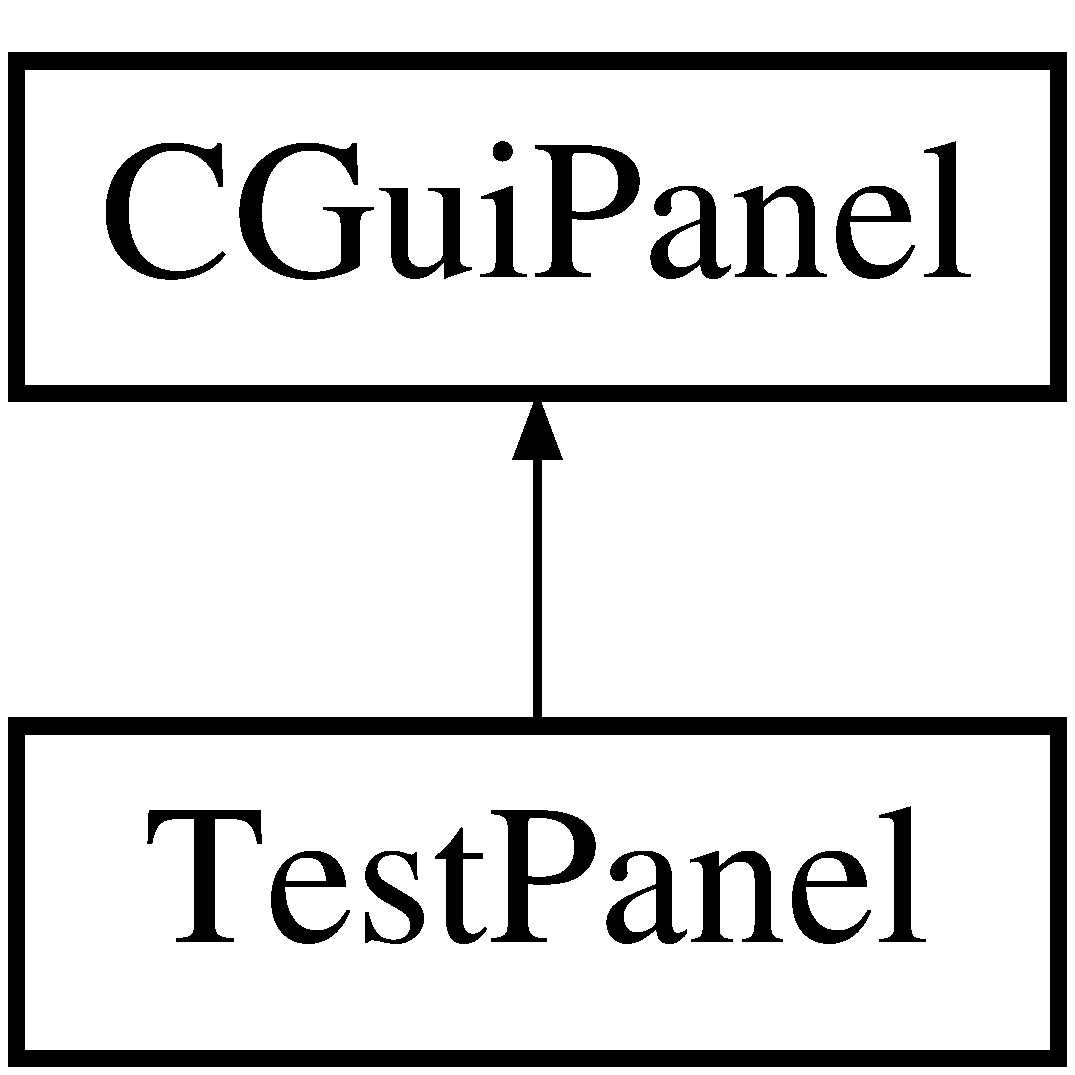
\includegraphics[height=2.000000cm]{class_test_panel}
\end{center}
\end{figure}
\subsection*{Public Member Functions}
\begin{DoxyCompactItemize}
\item 
\hypertarget{class_test_panel_abe43f13e886824378d7a59a4f784d078}{
{\bfseries TestPanel} (const \hyperlink{classvec2d}{vec2d} \&pos, const \hyperlink{classvec2d}{vec2d} \&size)}
\label{class_test_panel_abe43f13e886824378d7a59a4f784d078}

\item 
\hypertarget{class_test_panel_a84c91fe6c8223ec2cadf4c296f274c22}{
virtual void {\bfseries draw} ()}
\label{class_test_panel_a84c91fe6c8223ec2cadf4c296f274c22}

\item 
\hypertarget{class_test_panel_ae8b251d87c6169943e7e4ece3f1fe3c7}{
virtual void {\bfseries onMouseDown} (const \hyperlink{classvec2d}{vec2d} \&position, MouseButton button)}
\label{class_test_panel_ae8b251d87c6169943e7e4ece3f1fe3c7}

\item 
\hypertarget{class_test_panel_a7d4a569a0e32b459cbf3c287b99fa3a4}{
virtual void {\bfseries onMouseUp} (const \hyperlink{classvec2d}{vec2d} \&position, MouseButton button)}
\label{class_test_panel_a7d4a569a0e32b459cbf3c287b99fa3a4}

\item 
\hypertarget{class_test_panel_a604f62887198762cc29b6365155e000d}{
virtual void {\bfseries onMouseOver} ()}
\label{class_test_panel_a604f62887198762cc29b6365155e000d}

\item 
\hypertarget{class_test_panel_afb28903b1775fa90bdcee423a1b90640}{
virtual void {\bfseries onMouseOut} ()}
\label{class_test_panel_afb28903b1775fa90bdcee423a1b90640}

\end{DoxyCompactItemize}


The documentation for this class was generated from the following files:\begin{DoxyCompactItemize}
\item 
src/gui/TestPanel.h\item 
src/gui/TestPanel.cpp\end{DoxyCompactItemize}

\hypertarget{struct_t_t___c_map_info__}{
\section{TT\_\-CMapInfo\_\- Struct Reference}
\label{struct_t_t___c_map_info__}\index{TT\_\-CMapInfo\_\-@{TT\_\-CMapInfo\_\-}}
}
\subsection*{Public Attributes}
\begin{DoxyCompactItemize}
\item 
\hypertarget{struct_t_t___c_map_info___a4096f460af57f87cb9434a411c502d86}{
FT\_\-ULong {\bfseries language}}
\label{struct_t_t___c_map_info___a4096f460af57f87cb9434a411c502d86}

\item 
\hypertarget{struct_t_t___c_map_info___a122d56b4755597f134fcf4865cb0a4fc}{
FT\_\-Long {\bfseries format}}
\label{struct_t_t___c_map_info___a122d56b4755597f134fcf4865cb0a4fc}

\end{DoxyCompactItemize}


The documentation for this struct was generated from the following file:\begin{DoxyCompactItemize}
\item 
src/libs/freetype/internal/services/svttcmap.h\end{DoxyCompactItemize}

\hypertarget{struct_t_t___face_rec__}{
\section{TT\_\-FaceRec\_\- Struct Reference}
\label{struct_t_t___face_rec__}\index{TT\_\-FaceRec\_\-@{TT\_\-FaceRec\_\-}}
}
\subsection*{Public Attributes}
\begin{DoxyCompactItemize}
\item 
\hypertarget{struct_t_t___face_rec___ab07a1f6ce2cffe73a5501fb33164ae74}{
\hyperlink{struct_f_t___face_rec__}{FT\_\-FaceRec} {\bfseries root}}
\label{struct_t_t___face_rec___ab07a1f6ce2cffe73a5501fb33164ae74}

\item 
\hypertarget{struct_t_t___face_rec___a9cde4ce9550411379eef0791afef8943}{
TTC\_\-HeaderRec {\bfseries ttc\_\-header}}
\label{struct_t_t___face_rec___a9cde4ce9550411379eef0791afef8943}

\item 
\hypertarget{struct_t_t___face_rec___ae492c009d7c3dd1b7279f6596edb84af}{
FT\_\-ULong {\bfseries format\_\-tag}}
\label{struct_t_t___face_rec___ae492c009d7c3dd1b7279f6596edb84af}

\item 
\hypertarget{struct_t_t___face_rec___aa32df24e9bbbbc72117bfeb964028b6e}{
FT\_\-UShort {\bfseries num\_\-tables}}
\label{struct_t_t___face_rec___aa32df24e9bbbbc72117bfeb964028b6e}

\item 
\hypertarget{struct_t_t___face_rec___ae4480c53c6414c74919fc99c9192adfe}{
\hyperlink{struct_t_t___table_rec__}{TT\_\-Table} {\bfseries dir\_\-tables}}
\label{struct_t_t___face_rec___ae4480c53c6414c74919fc99c9192adfe}

\item 
\hypertarget{struct_t_t___face_rec___ac5fc04850d7b223029891601ed605b34}{
TT\_\-Header {\bfseries header}}
\label{struct_t_t___face_rec___ac5fc04850d7b223029891601ed605b34}

\item 
\hypertarget{struct_t_t___face_rec___a784d2ca39e9717da0661f5fd59dffc58}{
\hyperlink{struct_t_t___hori_header__}{TT\_\-HoriHeader} {\bfseries horizontal}}
\label{struct_t_t___face_rec___a784d2ca39e9717da0661f5fd59dffc58}

\item 
\hypertarget{struct_t_t___face_rec___a1bacbea2875d5fda567a5f561773035d}{
\hyperlink{struct_t_t___max_profile__}{TT\_\-MaxProfile} {\bfseries max\_\-profile}}
\label{struct_t_t___face_rec___a1bacbea2875d5fda567a5f561773035d}

\item 
\hypertarget{struct_t_t___face_rec___a43e1c7d3fd3f43ddd7b1bba243bf10bc}{
FT\_\-Bool {\bfseries vertical\_\-info}}
\label{struct_t_t___face_rec___a43e1c7d3fd3f43ddd7b1bba243bf10bc}

\item 
\hypertarget{struct_t_t___face_rec___a04fc41d3860163177a7e0a9bcf71ccf4}{
\hyperlink{struct_t_t___vert_header__}{TT\_\-VertHeader} {\bfseries vertical}}
\label{struct_t_t___face_rec___a04fc41d3860163177a7e0a9bcf71ccf4}

\item 
\hypertarget{struct_t_t___face_rec___ae73033d211e0ac91396e6bb22d594fab}{
FT\_\-UShort {\bfseries num\_\-names}}
\label{struct_t_t___face_rec___ae73033d211e0ac91396e6bb22d594fab}

\item 
\hypertarget{struct_t_t___face_rec___a33d114b43e6646893f15d39065b77e8c}{
\hyperlink{struct_t_t___name_table_rec__}{TT\_\-NameTableRec} {\bfseries name\_\-table}}
\label{struct_t_t___face_rec___a33d114b43e6646893f15d39065b77e8c}

\item 
\hypertarget{struct_t_t___face_rec___a5371adcbd62ade9b74e5f24a03ef09f2}{
\hyperlink{struct_t_t___o_s2__}{TT\_\-OS2} {\bfseries os2}}
\label{struct_t_t___face_rec___a5371adcbd62ade9b74e5f24a03ef09f2}

\item 
\hypertarget{struct_t_t___face_rec___a598bb9ada92970931585dc51878cf2cd}{
\hyperlink{struct_t_t___postscript__}{TT\_\-Postscript} {\bfseries postscript}}
\label{struct_t_t___face_rec___a598bb9ada92970931585dc51878cf2cd}

\item 
\hypertarget{struct_t_t___face_rec___a07bfd99f7725a1fb5f27b44a126a46ba}{
FT\_\-Byte $\ast$ {\bfseries cmap\_\-table}}
\label{struct_t_t___face_rec___a07bfd99f7725a1fb5f27b44a126a46ba}

\item 
\hypertarget{struct_t_t___face_rec___a4d2e127541e4f223c0b6c5d5aca4c8c5}{
FT\_\-ULong {\bfseries cmap\_\-size}}
\label{struct_t_t___face_rec___a4d2e127541e4f223c0b6c5d5aca4c8c5}

\item 
\hypertarget{struct_t_t___face_rec___a3e2e3599abb7737179dbb2fbbd15355d}{
TT\_\-Loader\_\-GotoTableFunc {\bfseries goto\_\-table}}
\label{struct_t_t___face_rec___a3e2e3599abb7737179dbb2fbbd15355d}

\item 
\hypertarget{struct_t_t___face_rec___a67cce5f4da277e6c8a47d8efe95bc58c}{
TT\_\-Loader\_\-StartGlyphFunc {\bfseries access\_\-glyph\_\-frame}}
\label{struct_t_t___face_rec___a67cce5f4da277e6c8a47d8efe95bc58c}

\item 
\hypertarget{struct_t_t___face_rec___ac86fbd960fe6c919eb82cd7233655894}{
TT\_\-Loader\_\-EndGlyphFunc {\bfseries forget\_\-glyph\_\-frame}}
\label{struct_t_t___face_rec___ac86fbd960fe6c919eb82cd7233655894}

\item 
\hypertarget{struct_t_t___face_rec___a343db3c51a3047324fea455ac06d7cb3}{
TT\_\-Loader\_\-ReadGlyphFunc {\bfseries read\_\-glyph\_\-header}}
\label{struct_t_t___face_rec___a343db3c51a3047324fea455ac06d7cb3}

\item 
\hypertarget{struct_t_t___face_rec___aa9f550ad4e10d8232cdd3427e02e7603}{
TT\_\-Loader\_\-ReadGlyphFunc {\bfseries read\_\-simple\_\-glyph}}
\label{struct_t_t___face_rec___aa9f550ad4e10d8232cdd3427e02e7603}

\item 
\hypertarget{struct_t_t___face_rec___ac261cd70ce36c35c615fc5e2319b40c4}{
TT\_\-Loader\_\-ReadGlyphFunc {\bfseries read\_\-composite\_\-glyph}}
\label{struct_t_t___face_rec___ac261cd70ce36c35c615fc5e2319b40c4}

\item 
\hypertarget{struct_t_t___face_rec___a4c198db893da1900ee0384969d10f9f6}{
void $\ast$ {\bfseries sfnt}}
\label{struct_t_t___face_rec___a4c198db893da1900ee0384969d10f9f6}

\item 
\hypertarget{struct_t_t___face_rec___a68cd8f2554793512af611422092b4814}{
void $\ast$ {\bfseries psnames}}
\label{struct_t_t___face_rec___a68cd8f2554793512af611422092b4814}

\item 
\hypertarget{struct_t_t___face_rec___a042468253b53931f4901ac47e37fbe14}{
\hyperlink{struct_t_t___gasp__}{TT\_\-GaspRec} {\bfseries gasp}}
\label{struct_t_t___face_rec___a042468253b53931f4901ac47e37fbe14}

\item 
\hypertarget{struct_t_t___face_rec___a18faed293bc94ac00fa7612b175adc0e}{
\hyperlink{struct_t_t___p_c_l_t__}{TT\_\-PCLT} {\bfseries pclt}}
\label{struct_t_t___face_rec___a18faed293bc94ac00fa7612b175adc0e}

\item 
\hypertarget{struct_t_t___face_rec___a5437fbf3ee625e001c28ec975326922a}{
FT\_\-ULong {\bfseries num\_\-sbit\_\-scales}}
\label{struct_t_t___face_rec___a5437fbf3ee625e001c28ec975326922a}

\item 
\hypertarget{struct_t_t___face_rec___a13215cb0365ee61c889385919fbd381f}{
\hyperlink{struct_t_t___s_bit___scale_rec__}{TT\_\-SBit\_\-Scale} {\bfseries sbit\_\-scales}}
\label{struct_t_t___face_rec___a13215cb0365ee61c889385919fbd381f}

\item 
\hypertarget{struct_t_t___face_rec___a875e8db9ffdf04b9e157c801c56921d0}{
\hyperlink{struct_t_t___post___names_rec__}{TT\_\-Post\_\-NamesRec} {\bfseries postscript\_\-names}}
\label{struct_t_t___face_rec___a875e8db9ffdf04b9e157c801c56921d0}

\item 
\hypertarget{struct_t_t___face_rec___ae0f510b460d6af3d62ce4c6b83247a39}{
FT\_\-ULong {\bfseries font\_\-program\_\-size}}
\label{struct_t_t___face_rec___ae0f510b460d6af3d62ce4c6b83247a39}

\item 
\hypertarget{struct_t_t___face_rec___a74268c6131bd14019910ad63e465231d}{
FT\_\-Byte $\ast$ {\bfseries font\_\-program}}
\label{struct_t_t___face_rec___a74268c6131bd14019910ad63e465231d}

\item 
\hypertarget{struct_t_t___face_rec___aeebca91e7b062ab0d1e149fb45257a6d}{
FT\_\-ULong {\bfseries cvt\_\-program\_\-size}}
\label{struct_t_t___face_rec___aeebca91e7b062ab0d1e149fb45257a6d}

\item 
\hypertarget{struct_t_t___face_rec___a6644124501481504fb315ba0395caa25}{
FT\_\-Byte $\ast$ {\bfseries cvt\_\-program}}
\label{struct_t_t___face_rec___a6644124501481504fb315ba0395caa25}

\item 
\hypertarget{struct_t_t___face_rec___a7508fd247ba7dba3087d09be4be7ebe4}{
FT\_\-ULong {\bfseries cvt\_\-size}}
\label{struct_t_t___face_rec___a7508fd247ba7dba3087d09be4be7ebe4}

\item 
\hypertarget{struct_t_t___face_rec___a191980a2e844052d746ea2e6432e927f}{
FT\_\-Short $\ast$ {\bfseries cvt}}
\label{struct_t_t___face_rec___a191980a2e844052d746ea2e6432e927f}

\item 
\hypertarget{struct_t_t___face_rec___a98b686a62bd5c8f45963a5c8742c095d}{
TT\_\-Interpreter {\bfseries interpreter}}
\label{struct_t_t___face_rec___a98b686a62bd5c8f45963a5c8742c095d}

\item 
\hypertarget{struct_t_t___face_rec___ab1ffe97c9ad4f20c71069b6b9bf005ee}{
\hyperlink{struct_f_t___generic__}{FT\_\-Generic} {\bfseries extra}}
\label{struct_t_t___face_rec___ab1ffe97c9ad4f20c71069b6b9bf005ee}

\item 
\hypertarget{struct_t_t___face_rec___a6e331e306d911cb437665b1b79b9a810}{
const char $\ast$ {\bfseries postscript\_\-name}}
\label{struct_t_t___face_rec___a6e331e306d911cb437665b1b79b9a810}

\item 
\hypertarget{struct_t_t___face_rec___a0bf0c5a8ce8e4f940eef826be23b918c}{
FT\_\-ULong {\bfseries glyf\_\-len}}
\label{struct_t_t___face_rec___a0bf0c5a8ce8e4f940eef826be23b918c}

\item 
\hypertarget{struct_t_t___face_rec___a06f8cb650c942b5c2b1d0f57cab66ba9}{
FT\_\-Byte $\ast$ {\bfseries horz\_\-metrics}}
\label{struct_t_t___face_rec___a06f8cb650c942b5c2b1d0f57cab66ba9}

\item 
\hypertarget{struct_t_t___face_rec___a8646a1f004307b49217459dc9284dc40}{
FT\_\-ULong {\bfseries horz\_\-metrics\_\-size}}
\label{struct_t_t___face_rec___a8646a1f004307b49217459dc9284dc40}

\item 
\hypertarget{struct_t_t___face_rec___affbbe1d319e871c4f075e70a931962c4}{
FT\_\-Byte $\ast$ {\bfseries vert\_\-metrics}}
\label{struct_t_t___face_rec___affbbe1d319e871c4f075e70a931962c4}

\item 
\hypertarget{struct_t_t___face_rec___aa72d0b40f0d0f3a21ba27a0deab1015f}{
FT\_\-ULong {\bfseries vert\_\-metrics\_\-size}}
\label{struct_t_t___face_rec___aa72d0b40f0d0f3a21ba27a0deab1015f}

\item 
\hypertarget{struct_t_t___face_rec___a26060b7a02227fb625a05b9e24ba5eea}{
FT\_\-ULong {\bfseries num\_\-locations}}
\label{struct_t_t___face_rec___a26060b7a02227fb625a05b9e24ba5eea}

\item 
\hypertarget{struct_t_t___face_rec___a12698e87c7be6955130a8c93592c71f7}{
FT\_\-Byte $\ast$ {\bfseries glyph\_\-locations}}
\label{struct_t_t___face_rec___a12698e87c7be6955130a8c93592c71f7}

\item 
\hypertarget{struct_t_t___face_rec___a67a5d79a4677d251c08c7ce26ccbc606}{
FT\_\-Byte $\ast$ {\bfseries hdmx\_\-table}}
\label{struct_t_t___face_rec___a67a5d79a4677d251c08c7ce26ccbc606}

\item 
\hypertarget{struct_t_t___face_rec___a2819ef14106792c3fa3b3924caf1ac00}{
FT\_\-ULong {\bfseries hdmx\_\-table\_\-size}}
\label{struct_t_t___face_rec___a2819ef14106792c3fa3b3924caf1ac00}

\item 
\hypertarget{struct_t_t___face_rec___ac4d9c1949e6e2c8b8d3074195bc5b03a}{
FT\_\-UInt {\bfseries hdmx\_\-record\_\-count}}
\label{struct_t_t___face_rec___ac4d9c1949e6e2c8b8d3074195bc5b03a}

\item 
\hypertarget{struct_t_t___face_rec___a3ae2a9ed9075cd1d765496d7e54fa23b}{
FT\_\-ULong {\bfseries hdmx\_\-record\_\-size}}
\label{struct_t_t___face_rec___a3ae2a9ed9075cd1d765496d7e54fa23b}

\item 
\hypertarget{struct_t_t___face_rec___ac7a599ad1d8f4c9fde887f95d17e862b}{
FT\_\-Byte $\ast$ {\bfseries hdmx\_\-record\_\-sizes}}
\label{struct_t_t___face_rec___ac7a599ad1d8f4c9fde887f95d17e862b}

\item 
\hypertarget{struct_t_t___face_rec___ade433be10a16d4193e3527c5b1b73fcd}{
FT\_\-Byte $\ast$ {\bfseries sbit\_\-table}}
\label{struct_t_t___face_rec___ade433be10a16d4193e3527c5b1b73fcd}

\item 
\hypertarget{struct_t_t___face_rec___ae16d371d8ca112b3e1f4cd35c256c829}{
FT\_\-ULong {\bfseries sbit\_\-table\_\-size}}
\label{struct_t_t___face_rec___ae16d371d8ca112b3e1f4cd35c256c829}

\item 
\hypertarget{struct_t_t___face_rec___a763b677d9356ea3ba116d113ebcb39e1}{
FT\_\-UInt {\bfseries sbit\_\-num\_\-strikes}}
\label{struct_t_t___face_rec___a763b677d9356ea3ba116d113ebcb39e1}

\item 
\hypertarget{struct_t_t___face_rec___ae445fbf0615a96f81b034b77ae1343a2}{
FT\_\-Byte $\ast$ {\bfseries kern\_\-table}}
\label{struct_t_t___face_rec___ae445fbf0615a96f81b034b77ae1343a2}

\item 
\hypertarget{struct_t_t___face_rec___acfef0fabbe95af382fb0710edfe98887}{
FT\_\-ULong {\bfseries kern\_\-table\_\-size}}
\label{struct_t_t___face_rec___acfef0fabbe95af382fb0710edfe98887}

\item 
\hypertarget{struct_t_t___face_rec___a9c5b27564d0c22e0ee6edd7b6dc675c0}{
FT\_\-UInt {\bfseries num\_\-kern\_\-tables}}
\label{struct_t_t___face_rec___a9c5b27564d0c22e0ee6edd7b6dc675c0}

\item 
\hypertarget{struct_t_t___face_rec___a5f97232ee6773a57ef8734555cc960e1}{
FT\_\-UInt32 {\bfseries kern\_\-avail\_\-bits}}
\label{struct_t_t___face_rec___a5f97232ee6773a57ef8734555cc960e1}

\item 
\hypertarget{struct_t_t___face_rec___a810b4e002ebbdfcb44005cb69b09a917}{
FT\_\-UInt32 {\bfseries kern\_\-order\_\-bits}}
\label{struct_t_t___face_rec___a810b4e002ebbdfcb44005cb69b09a917}

\item 
\hypertarget{struct_t_t___face_rec___a5ff62c77d90743e333ca8dfa7d382f22}{
FT\_\-ULong {\bfseries horz\_\-metrics\_\-offset}}
\label{struct_t_t___face_rec___a5ff62c77d90743e333ca8dfa7d382f22}

\item 
\hypertarget{struct_t_t___face_rec___a33baf2e26d533d82f06875361fd423d1}{
FT\_\-ULong {\bfseries vert\_\-metrics\_\-offset}}
\label{struct_t_t___face_rec___a33baf2e26d533d82f06875361fd423d1}

\end{DoxyCompactItemize}


The documentation for this struct was generated from the following file:\begin{DoxyCompactItemize}
\item 
src/libs/freetype/internal/tttypes.h\end{DoxyCompactItemize}

\hypertarget{struct_t_t___gasp__}{
\section{TT\_\-Gasp\_\- Struct Reference}
\label{struct_t_t___gasp__}\index{TT\_\-Gasp\_\-@{TT\_\-Gasp\_\-}}
}
\subsection*{Public Attributes}
\begin{DoxyCompactItemize}
\item 
\hypertarget{struct_t_t___gasp___a0166777999a11a32068418ed6cf0caf8}{
FT\_\-UShort {\bfseries version}}
\label{struct_t_t___gasp___a0166777999a11a32068418ed6cf0caf8}

\item 
\hypertarget{struct_t_t___gasp___a03f6dc693ebee0fedc055ac0981ee776}{
FT\_\-UShort {\bfseries numRanges}}
\label{struct_t_t___gasp___a03f6dc693ebee0fedc055ac0981ee776}

\item 
\hypertarget{struct_t_t___gasp___a50240e84cfd7fc79ae1f2996ecb2a5d1}{
\hyperlink{struct_t_t___gasp_range_rec__}{TT\_\-GaspRange} {\bfseries gaspRanges}}
\label{struct_t_t___gasp___a50240e84cfd7fc79ae1f2996ecb2a5d1}

\end{DoxyCompactItemize}


The documentation for this struct was generated from the following file:\begin{DoxyCompactItemize}
\item 
src/libs/freetype/internal/tttypes.h\end{DoxyCompactItemize}

\hypertarget{struct_t_t___gasp_range_rec__}{
\section{TT\_\-GaspRangeRec\_\- Struct Reference}
\label{struct_t_t___gasp_range_rec__}\index{TT\_\-GaspRangeRec\_\-@{TT\_\-GaspRangeRec\_\-}}
}
\subsection*{Public Attributes}
\begin{DoxyCompactItemize}
\item 
\hypertarget{struct_t_t___gasp_range_rec___aa3fab31f6c0659b4deff402e210e15c9}{
FT\_\-UShort {\bfseries maxPPEM}}
\label{struct_t_t___gasp_range_rec___aa3fab31f6c0659b4deff402e210e15c9}

\item 
\hypertarget{struct_t_t___gasp_range_rec___a9fc298dc0e46d31507728ae25585118d}{
FT\_\-UShort {\bfseries gaspFlag}}
\label{struct_t_t___gasp_range_rec___a9fc298dc0e46d31507728ae25585118d}

\end{DoxyCompactItemize}


The documentation for this struct was generated from the following file:\begin{DoxyCompactItemize}
\item 
src/libs/freetype/internal/tttypes.h\end{DoxyCompactItemize}

\hypertarget{struct_t_t___glyph_zone_rec__}{
\section{TT\_\-GlyphZoneRec\_\- Struct Reference}
\label{struct_t_t___glyph_zone_rec__}\index{TT\_\-GlyphZoneRec\_\-@{TT\_\-GlyphZoneRec\_\-}}
}
\subsection*{Public Attributes}
\begin{DoxyCompactItemize}
\item 
\hypertarget{struct_t_t___glyph_zone_rec___adc8cac6d6d8475aa50946d6bc17fd345}{
FT\_\-Memory {\bfseries memory}}
\label{struct_t_t___glyph_zone_rec___adc8cac6d6d8475aa50946d6bc17fd345}

\item 
\hypertarget{struct_t_t___glyph_zone_rec___aa06aa1bfd1b7e2082552ea24f96c775e}{
FT\_\-UShort {\bfseries max\_\-points}}
\label{struct_t_t___glyph_zone_rec___aa06aa1bfd1b7e2082552ea24f96c775e}

\item 
\hypertarget{struct_t_t___glyph_zone_rec___a268ef8e7a7da1c077c762d04089b2605}{
FT\_\-UShort {\bfseries max\_\-contours}}
\label{struct_t_t___glyph_zone_rec___a268ef8e7a7da1c077c762d04089b2605}

\item 
\hypertarget{struct_t_t___glyph_zone_rec___a2acc389958f0e593f7eed29f7ca15b94}{
FT\_\-UShort {\bfseries n\_\-points}}
\label{struct_t_t___glyph_zone_rec___a2acc389958f0e593f7eed29f7ca15b94}

\item 
\hypertarget{struct_t_t___glyph_zone_rec___a1aa2ffa863fbd8a8985fe3e39e8bb92a}{
FT\_\-Short {\bfseries n\_\-contours}}
\label{struct_t_t___glyph_zone_rec___a1aa2ffa863fbd8a8985fe3e39e8bb92a}

\item 
\hypertarget{struct_t_t___glyph_zone_rec___a240879d0a1a6dd487b84f3b3723f9058}{
\hyperlink{struct_f_t___vector__}{FT\_\-Vector} $\ast$ {\bfseries org}}
\label{struct_t_t___glyph_zone_rec___a240879d0a1a6dd487b84f3b3723f9058}

\item 
\hypertarget{struct_t_t___glyph_zone_rec___a5dc4b386729ab85619a7132f69714991}{
\hyperlink{struct_f_t___vector__}{FT\_\-Vector} $\ast$ {\bfseries cur}}
\label{struct_t_t___glyph_zone_rec___a5dc4b386729ab85619a7132f69714991}

\item 
\hypertarget{struct_t_t___glyph_zone_rec___a4b4193dbae177435cb6515f9a0537fa0}{
\hyperlink{struct_f_t___vector__}{FT\_\-Vector} $\ast$ {\bfseries orus}}
\label{struct_t_t___glyph_zone_rec___a4b4193dbae177435cb6515f9a0537fa0}

\item 
\hypertarget{struct_t_t___glyph_zone_rec___ae816c5c1096e333741d3f3f9d3ae0a8f}{
FT\_\-Byte $\ast$ {\bfseries tags}}
\label{struct_t_t___glyph_zone_rec___ae816c5c1096e333741d3f3f9d3ae0a8f}

\item 
\hypertarget{struct_t_t___glyph_zone_rec___ad16498cac0d4d233dce009eb74d63de1}{
FT\_\-UShort $\ast$ {\bfseries contours}}
\label{struct_t_t___glyph_zone_rec___ad16498cac0d4d233dce009eb74d63de1}

\item 
\hypertarget{struct_t_t___glyph_zone_rec___a9d655be80b3e31652f69ede54458faaf}{
FT\_\-UShort {\bfseries first\_\-point}}
\label{struct_t_t___glyph_zone_rec___a9d655be80b3e31652f69ede54458faaf}

\end{DoxyCompactItemize}


The documentation for this struct was generated from the following file:\begin{DoxyCompactItemize}
\item 
src/libs/freetype/internal/tttypes.h\end{DoxyCompactItemize}

\hypertarget{struct_t_t___header__}{
\section{TT\_\-Header\_\- Struct Reference}
\label{struct_t_t___header__}\index{TT\_\-Header\_\-@{TT\_\-Header\_\-}}
}
\subsection*{Public Attributes}
\begin{DoxyCompactItemize}
\item 
\hypertarget{struct_t_t___header___ab14622e8f8f80ee8361f4847cf9c36e1}{
FT\_\-Fixed {\bfseries Table\_\-Version}}
\label{struct_t_t___header___ab14622e8f8f80ee8361f4847cf9c36e1}

\item 
\hypertarget{struct_t_t___header___aa5d0f9f88a7ffc755982a1a9dbb58f21}{
FT\_\-Fixed {\bfseries Font\_\-Revision}}
\label{struct_t_t___header___aa5d0f9f88a7ffc755982a1a9dbb58f21}

\item 
\hypertarget{struct_t_t___header___a5ca008fa01e9568769287febc2abd807}{
FT\_\-Long {\bfseries CheckSum\_\-Adjust}}
\label{struct_t_t___header___a5ca008fa01e9568769287febc2abd807}

\item 
\hypertarget{struct_t_t___header___a24e0dde7596c7303c8b8872feb1c221f}{
FT\_\-Long {\bfseries Magic\_\-Number}}
\label{struct_t_t___header___a24e0dde7596c7303c8b8872feb1c221f}

\item 
\hypertarget{struct_t_t___header___a9e81d0e6bf9a83ebf28f768d83559f38}{
FT\_\-UShort {\bfseries Flags}}
\label{struct_t_t___header___a9e81d0e6bf9a83ebf28f768d83559f38}

\item 
\hypertarget{struct_t_t___header___a594567319e6b6b5a823567279d26857d}{
FT\_\-UShort {\bfseries Units\_\-Per\_\-EM}}
\label{struct_t_t___header___a594567319e6b6b5a823567279d26857d}

\item 
\hypertarget{struct_t_t___header___a1e5d99f35ae2a604c6f54da94dc5105f}{
FT\_\-Long {\bfseries Created} \mbox{[}2\mbox{]}}
\label{struct_t_t___header___a1e5d99f35ae2a604c6f54da94dc5105f}

\item 
\hypertarget{struct_t_t___header___a48db8e244aee26da683240e67644619e}{
FT\_\-Long {\bfseries Modified} \mbox{[}2\mbox{]}}
\label{struct_t_t___header___a48db8e244aee26da683240e67644619e}

\item 
\hypertarget{struct_t_t___header___ae4553d76427d9f7a28595ed71897dcbb}{
FT\_\-Short {\bfseries xMin}}
\label{struct_t_t___header___ae4553d76427d9f7a28595ed71897dcbb}

\item 
\hypertarget{struct_t_t___header___ac6aad4966bac8a96c5bc48765b3d694a}{
FT\_\-Short {\bfseries yMin}}
\label{struct_t_t___header___ac6aad4966bac8a96c5bc48765b3d694a}

\item 
\hypertarget{struct_t_t___header___a593b9cc3e11532972a7fc96944dd1ae9}{
FT\_\-Short {\bfseries xMax}}
\label{struct_t_t___header___a593b9cc3e11532972a7fc96944dd1ae9}

\item 
\hypertarget{struct_t_t___header___a02d236cd8150c00e886a0c487c04dffa}{
FT\_\-Short {\bfseries yMax}}
\label{struct_t_t___header___a02d236cd8150c00e886a0c487c04dffa}

\item 
\hypertarget{struct_t_t___header___a82f2a5a836b802e44ff712b3afc8745c}{
FT\_\-UShort {\bfseries Mac\_\-Style}}
\label{struct_t_t___header___a82f2a5a836b802e44ff712b3afc8745c}

\item 
\hypertarget{struct_t_t___header___a1d20801c3482dee2529d294441ed9af3}{
FT\_\-UShort {\bfseries Lowest\_\-Rec\_\-PPEM}}
\label{struct_t_t___header___a1d20801c3482dee2529d294441ed9af3}

\item 
\hypertarget{struct_t_t___header___a1cb7d8a2a76ae1acda3ac94bcd555954}{
FT\_\-Short {\bfseries Font\_\-Direction}}
\label{struct_t_t___header___a1cb7d8a2a76ae1acda3ac94bcd555954}

\item 
\hypertarget{struct_t_t___header___a05a488607bfae319de096b4bd9cf8c6d}{
FT\_\-Short {\bfseries Index\_\-To\_\-Loc\_\-Format}}
\label{struct_t_t___header___a05a488607bfae319de096b4bd9cf8c6d}

\item 
\hypertarget{struct_t_t___header___adeeedce4bb708c3e068ed80366ec921d}{
FT\_\-Short {\bfseries Glyph\_\-Data\_\-Format}}
\label{struct_t_t___header___adeeedce4bb708c3e068ed80366ec921d}

\end{DoxyCompactItemize}


The documentation for this struct was generated from the following file:\begin{DoxyCompactItemize}
\item 
src/libs/freetype/tttables.h\end{DoxyCompactItemize}

\hypertarget{struct_t_t___hori_header__}{
\section{TT\_\-HoriHeader\_\- Struct Reference}
\label{struct_t_t___hori_header__}\index{TT\_\-HoriHeader\_\-@{TT\_\-HoriHeader\_\-}}
}
\subsection*{Public Attributes}
\begin{DoxyCompactItemize}
\item 
\hypertarget{struct_t_t___hori_header___a2d0967448b63db392e35b566196fef97}{
FT\_\-Fixed {\bfseries Version}}
\label{struct_t_t___hori_header___a2d0967448b63db392e35b566196fef97}

\item 
\hypertarget{struct_t_t___hori_header___a6f987c89428c93854dab06e506134249}{
FT\_\-Short {\bfseries Ascender}}
\label{struct_t_t___hori_header___a6f987c89428c93854dab06e506134249}

\item 
\hypertarget{struct_t_t___hori_header___ad5be55a98dfaa079a2aaa462034a1512}{
FT\_\-Short {\bfseries Descender}}
\label{struct_t_t___hori_header___ad5be55a98dfaa079a2aaa462034a1512}

\item 
\hypertarget{struct_t_t___hori_header___a4165055ed05e42a2e5eed805bfe3fd7d}{
FT\_\-Short {\bfseries Line\_\-Gap}}
\label{struct_t_t___hori_header___a4165055ed05e42a2e5eed805bfe3fd7d}

\item 
\hypertarget{struct_t_t___hori_header___a1ddad7e4c5e6fed50c073745961814da}{
FT\_\-UShort {\bfseries advance\_\-Width\_\-Max}}
\label{struct_t_t___hori_header___a1ddad7e4c5e6fed50c073745961814da}

\item 
\hypertarget{struct_t_t___hori_header___a0e2e2bf8ca0e18b610c4eae0a647fded}{
FT\_\-Short {\bfseries min\_\-Left\_\-Side\_\-Bearing}}
\label{struct_t_t___hori_header___a0e2e2bf8ca0e18b610c4eae0a647fded}

\item 
\hypertarget{struct_t_t___hori_header___a64144cdd595e8e8de119b78539bf2fa7}{
FT\_\-Short {\bfseries min\_\-Right\_\-Side\_\-Bearing}}
\label{struct_t_t___hori_header___a64144cdd595e8e8de119b78539bf2fa7}

\item 
\hypertarget{struct_t_t___hori_header___ab483cb323f9adc9d959209a42eb19957}{
FT\_\-Short {\bfseries xMax\_\-Extent}}
\label{struct_t_t___hori_header___ab483cb323f9adc9d959209a42eb19957}

\item 
\hypertarget{struct_t_t___hori_header___aeb43d92f56de424d8f28bd389973eca4}{
FT\_\-Short {\bfseries caret\_\-Slope\_\-Rise}}
\label{struct_t_t___hori_header___aeb43d92f56de424d8f28bd389973eca4}

\item 
\hypertarget{struct_t_t___hori_header___acce162ae0554006c11a3383bd3454d69}{
FT\_\-Short {\bfseries caret\_\-Slope\_\-Run}}
\label{struct_t_t___hori_header___acce162ae0554006c11a3383bd3454d69}

\item 
\hypertarget{struct_t_t___hori_header___a791ad767d54cc87e84d9b03d6739f0eb}{
FT\_\-Short {\bfseries caret\_\-Offset}}
\label{struct_t_t___hori_header___a791ad767d54cc87e84d9b03d6739f0eb}

\item 
\hypertarget{struct_t_t___hori_header___af2a2b374d8f81771fb75d3bdc96bcbf7}{
FT\_\-Short {\bfseries Reserved} \mbox{[}4\mbox{]}}
\label{struct_t_t___hori_header___af2a2b374d8f81771fb75d3bdc96bcbf7}

\item 
\hypertarget{struct_t_t___hori_header___a0ed857e9629d2dfb5350a6b5976bf933}{
FT\_\-Short {\bfseries metric\_\-Data\_\-Format}}
\label{struct_t_t___hori_header___a0ed857e9629d2dfb5350a6b5976bf933}

\item 
\hypertarget{struct_t_t___hori_header___aac3ecb9ba7c13436a663b91765e89647}{
FT\_\-UShort {\bfseries number\_\-Of\_\-HMetrics}}
\label{struct_t_t___hori_header___aac3ecb9ba7c13436a663b91765e89647}

\item 
\hypertarget{struct_t_t___hori_header___a3eeb5766b461e9563b659a30e775fcc2}{
void $\ast$ {\bfseries long\_\-metrics}}
\label{struct_t_t___hori_header___a3eeb5766b461e9563b659a30e775fcc2}

\item 
\hypertarget{struct_t_t___hori_header___ae39107c4cfc3e7c1871dbb304bbe4a5a}{
void $\ast$ {\bfseries short\_\-metrics}}
\label{struct_t_t___hori_header___ae39107c4cfc3e7c1871dbb304bbe4a5a}

\end{DoxyCompactItemize}


The documentation for this struct was generated from the following file:\begin{DoxyCompactItemize}
\item 
src/libs/freetype/tttables.h\end{DoxyCompactItemize}

\hypertarget{struct_t_t___loader_rec__}{
\section{TT\_\-LoaderRec\_\- Struct Reference}
\label{struct_t_t___loader_rec__}\index{TT\_\-LoaderRec\_\-@{TT\_\-LoaderRec\_\-}}
}
\subsection*{Public Attributes}
\begin{DoxyCompactItemize}
\item 
\hypertarget{struct_t_t___loader_rec___a03a83a2bdc0a10698a72ade8ae5700d2}{
\hyperlink{struct_f_t___face_rec__}{FT\_\-Face} {\bfseries face}}
\label{struct_t_t___loader_rec___a03a83a2bdc0a10698a72ade8ae5700d2}

\item 
\hypertarget{struct_t_t___loader_rec___a9b819b48f7c9d3efd4960700060ccefc}{
\hyperlink{struct_f_t___size_rec__}{FT\_\-Size} {\bfseries size}}
\label{struct_t_t___loader_rec___a9b819b48f7c9d3efd4960700060ccefc}

\item 
\hypertarget{struct_t_t___loader_rec___a7843d7a665f8535faadf1bf1ec87b683}{
\hyperlink{struct_f_t___glyph_slot_rec__}{FT\_\-GlyphSlot} {\bfseries glyph}}
\label{struct_t_t___loader_rec___a7843d7a665f8535faadf1bf1ec87b683}

\item 
\hypertarget{struct_t_t___loader_rec___a5c24ef5e731e4d9953be8ede99d6cf54}{
FT\_\-GlyphLoader {\bfseries gloader}}
\label{struct_t_t___loader_rec___a5c24ef5e731e4d9953be8ede99d6cf54}

\item 
\hypertarget{struct_t_t___loader_rec___a19ca6de6b384c1b6143275a485a3160f}{
FT\_\-ULong {\bfseries load\_\-flags}}
\label{struct_t_t___loader_rec___a19ca6de6b384c1b6143275a485a3160f}

\item 
\hypertarget{struct_t_t___loader_rec___a5486105cac09d372c0971c237585b135}{
FT\_\-UInt {\bfseries glyph\_\-index}}
\label{struct_t_t___loader_rec___a5486105cac09d372c0971c237585b135}

\item 
\hypertarget{struct_t_t___loader_rec___abb44841d62cecea6dd413be951eae241}{
\hyperlink{struct_f_t___stream_rec__}{FT\_\-Stream} {\bfseries stream}}
\label{struct_t_t___loader_rec___abb44841d62cecea6dd413be951eae241}

\item 
\hypertarget{struct_t_t___loader_rec___a43c6befa8051373b8d18e6a60c6bee30}{
FT\_\-Int {\bfseries byte\_\-len}}
\label{struct_t_t___loader_rec___a43c6befa8051373b8d18e6a60c6bee30}

\item 
\hypertarget{struct_t_t___loader_rec___a829910a8b1d82620efa96bf25a119e35}{
FT\_\-Short {\bfseries n\_\-contours}}
\label{struct_t_t___loader_rec___a829910a8b1d82620efa96bf25a119e35}

\item 
\hypertarget{struct_t_t___loader_rec___ac9bb4330b5dac24623f69bd4626939da}{
\hyperlink{struct_f_t___b_box__}{FT\_\-BBox} {\bfseries bbox}}
\label{struct_t_t___loader_rec___ac9bb4330b5dac24623f69bd4626939da}

\item 
\hypertarget{struct_t_t___loader_rec___ad03cc327dd6ec53390a069425e81bf4d}{
FT\_\-Int {\bfseries left\_\-bearing}}
\label{struct_t_t___loader_rec___ad03cc327dd6ec53390a069425e81bf4d}

\item 
\hypertarget{struct_t_t___loader_rec___a6d9d5002ddfe94c070a6ba1c03be1b85}{
FT\_\-Int {\bfseries advance}}
\label{struct_t_t___loader_rec___a6d9d5002ddfe94c070a6ba1c03be1b85}

\item 
\hypertarget{struct_t_t___loader_rec___acad580f20d35eba80cbb08eb3b3e8079}{
FT\_\-Int {\bfseries linear}}
\label{struct_t_t___loader_rec___acad580f20d35eba80cbb08eb3b3e8079}

\item 
\hypertarget{struct_t_t___loader_rec___a9ecbb843ee8715143223f736c0cccadc}{
FT\_\-Bool {\bfseries linear\_\-def}}
\label{struct_t_t___loader_rec___a9ecbb843ee8715143223f736c0cccadc}

\item 
\hypertarget{struct_t_t___loader_rec___a0e091a351780ac808240d8c55daf47ab}{
FT\_\-Bool {\bfseries preserve\_\-pps}}
\label{struct_t_t___loader_rec___a0e091a351780ac808240d8c55daf47ab}

\item 
\hypertarget{struct_t_t___loader_rec___aa4764ae2c27d976e378e9d6228b828e9}{
\hyperlink{struct_f_t___vector__}{FT\_\-Vector} {\bfseries pp1}}
\label{struct_t_t___loader_rec___aa4764ae2c27d976e378e9d6228b828e9}

\item 
\hypertarget{struct_t_t___loader_rec___a833a56d41e708dfa971c9efb5a4267e1}{
\hyperlink{struct_f_t___vector__}{FT\_\-Vector} {\bfseries pp2}}
\label{struct_t_t___loader_rec___a833a56d41e708dfa971c9efb5a4267e1}

\item 
\hypertarget{struct_t_t___loader_rec___a54954750de6323be405073475c3e9c67}{
FT\_\-ULong {\bfseries glyf\_\-offset}}
\label{struct_t_t___loader_rec___a54954750de6323be405073475c3e9c67}

\item 
\hypertarget{struct_t_t___loader_rec___ab714636e13a1a9211bf2e4734eba8a1d}{
\hyperlink{struct_t_t___glyph_zone_rec__}{TT\_\-GlyphZoneRec} {\bfseries base}}
\label{struct_t_t___loader_rec___ab714636e13a1a9211bf2e4734eba8a1d}

\item 
\hypertarget{struct_t_t___loader_rec___aaa594deb371418c6cb932f318a8631ce}{
\hyperlink{struct_t_t___glyph_zone_rec__}{TT\_\-GlyphZoneRec} {\bfseries zone}}
\label{struct_t_t___loader_rec___aaa594deb371418c6cb932f318a8631ce}

\item 
\hypertarget{struct_t_t___loader_rec___a22cae1f510e891a525092d33b373cc01}{
TT\_\-ExecContext {\bfseries exec}}
\label{struct_t_t___loader_rec___a22cae1f510e891a525092d33b373cc01}

\item 
\hypertarget{struct_t_t___loader_rec___aaf1018107d5166a684604fde765b625a}{
FT\_\-Byte $\ast$ {\bfseries instructions}}
\label{struct_t_t___loader_rec___aaf1018107d5166a684604fde765b625a}

\item 
\hypertarget{struct_t_t___loader_rec___a56c391d36a6391e8395cd09bc972b8b0}{
FT\_\-ULong {\bfseries ins\_\-pos}}
\label{struct_t_t___loader_rec___a56c391d36a6391e8395cd09bc972b8b0}

\item 
\hypertarget{struct_t_t___loader_rec___a52009bf0f7ac51833b9fcba1b3bf0ffd}{
void $\ast$ {\bfseries other}}
\label{struct_t_t___loader_rec___a52009bf0f7ac51833b9fcba1b3bf0ffd}

\item 
\hypertarget{struct_t_t___loader_rec___a00c9197ba5abd4e677f116423793a9f4}{
FT\_\-Int {\bfseries top\_\-bearing}}
\label{struct_t_t___loader_rec___a00c9197ba5abd4e677f116423793a9f4}

\item 
\hypertarget{struct_t_t___loader_rec___aec9d10cfbe0ced3fff990bb9e936e95d}{
FT\_\-Int {\bfseries vadvance}}
\label{struct_t_t___loader_rec___aec9d10cfbe0ced3fff990bb9e936e95d}

\item 
\hypertarget{struct_t_t___loader_rec___a262052584bfb1ec7e6e801f71169093b}{
\hyperlink{struct_f_t___vector__}{FT\_\-Vector} {\bfseries pp3}}
\label{struct_t_t___loader_rec___a262052584bfb1ec7e6e801f71169093b}

\item 
\hypertarget{struct_t_t___loader_rec___a0608203207c3fc735046b8baef4b9201}{
\hyperlink{struct_f_t___vector__}{FT\_\-Vector} {\bfseries pp4}}
\label{struct_t_t___loader_rec___a0608203207c3fc735046b8baef4b9201}

\item 
\hypertarget{struct_t_t___loader_rec___a6769a96f37ca22801f6199937cbe9ca7}{
FT\_\-Byte $\ast$ {\bfseries cursor}}
\label{struct_t_t___loader_rec___a6769a96f37ca22801f6199937cbe9ca7}

\item 
\hypertarget{struct_t_t___loader_rec___a1b07761e8ea436c38b4c42117a00a0ff}{
FT\_\-Byte $\ast$ {\bfseries limit}}
\label{struct_t_t___loader_rec___a1b07761e8ea436c38b4c42117a00a0ff}

\end{DoxyCompactItemize}


The documentation for this struct was generated from the following file:\begin{DoxyCompactItemize}
\item 
src/libs/freetype/internal/tttypes.h\end{DoxyCompactItemize}

\hypertarget{struct_t_t___long_metrics_rec__}{
\section{TT\_\-LongMetricsRec\_\- Struct Reference}
\label{struct_t_t___long_metrics_rec__}\index{TT\_\-LongMetricsRec\_\-@{TT\_\-LongMetricsRec\_\-}}
}
\subsection*{Public Attributes}
\begin{DoxyCompactItemize}
\item 
\hypertarget{struct_t_t___long_metrics_rec___a47100e42b52486bc374f80ed2795361d}{
FT\_\-UShort {\bfseries advance}}
\label{struct_t_t___long_metrics_rec___a47100e42b52486bc374f80ed2795361d}

\item 
\hypertarget{struct_t_t___long_metrics_rec___a0d74e3eb8611b0a5e89e338af35be4da}{
FT\_\-Short {\bfseries bearing}}
\label{struct_t_t___long_metrics_rec___a0d74e3eb8611b0a5e89e338af35be4da}

\end{DoxyCompactItemize}


The documentation for this struct was generated from the following file:\begin{DoxyCompactItemize}
\item 
src/libs/freetype/internal/tttypes.h\end{DoxyCompactItemize}

\hypertarget{struct_t_t___max_profile__}{
\section{TT\_\-MaxProfile\_\- Struct Reference}
\label{struct_t_t___max_profile__}\index{TT\_\-MaxProfile\_\-@{TT\_\-MaxProfile\_\-}}
}
\subsection*{Public Attributes}
\begin{DoxyCompactItemize}
\item 
\hypertarget{struct_t_t___max_profile___a59618f7c572dadc58e883d32dea46380}{
FT\_\-Fixed {\bfseries version}}
\label{struct_t_t___max_profile___a59618f7c572dadc58e883d32dea46380}

\item 
\hypertarget{struct_t_t___max_profile___a6ec14b34978f24173d50ab556613ade5}{
FT\_\-UShort {\bfseries numGlyphs}}
\label{struct_t_t___max_profile___a6ec14b34978f24173d50ab556613ade5}

\item 
\hypertarget{struct_t_t___max_profile___a218fa149a195e9afa1738ef5aef07aa1}{
FT\_\-UShort {\bfseries maxPoints}}
\label{struct_t_t___max_profile___a218fa149a195e9afa1738ef5aef07aa1}

\item 
\hypertarget{struct_t_t___max_profile___a5af98bd8149008d0a33b61d9730262a9}{
FT\_\-UShort {\bfseries maxContours}}
\label{struct_t_t___max_profile___a5af98bd8149008d0a33b61d9730262a9}

\item 
\hypertarget{struct_t_t___max_profile___aafc5ef3f58254792c353a6fb3b3a044e}{
FT\_\-UShort {\bfseries maxCompositePoints}}
\label{struct_t_t___max_profile___aafc5ef3f58254792c353a6fb3b3a044e}

\item 
\hypertarget{struct_t_t___max_profile___a956e7c44e46a8aeb6d419b8550d1e556}{
FT\_\-UShort {\bfseries maxCompositeContours}}
\label{struct_t_t___max_profile___a956e7c44e46a8aeb6d419b8550d1e556}

\item 
\hypertarget{struct_t_t___max_profile___a07213312ec7b821a53a17d90930a478a}{
FT\_\-UShort {\bfseries maxZones}}
\label{struct_t_t___max_profile___a07213312ec7b821a53a17d90930a478a}

\item 
\hypertarget{struct_t_t___max_profile___a907e28d69ad5e2a2c446e3eae8301af2}{
FT\_\-UShort {\bfseries maxTwilightPoints}}
\label{struct_t_t___max_profile___a907e28d69ad5e2a2c446e3eae8301af2}

\item 
\hypertarget{struct_t_t___max_profile___a502a8579e3d358f3c00776ed0cc8a168}{
FT\_\-UShort {\bfseries maxStorage}}
\label{struct_t_t___max_profile___a502a8579e3d358f3c00776ed0cc8a168}

\item 
\hypertarget{struct_t_t___max_profile___acc24e822a62bbfaa86d36f691fcde60b}{
FT\_\-UShort {\bfseries maxFunctionDefs}}
\label{struct_t_t___max_profile___acc24e822a62bbfaa86d36f691fcde60b}

\item 
\hypertarget{struct_t_t___max_profile___a3f7bd433baede417293415cf60f20d8f}{
FT\_\-UShort {\bfseries maxInstructionDefs}}
\label{struct_t_t___max_profile___a3f7bd433baede417293415cf60f20d8f}

\item 
\hypertarget{struct_t_t___max_profile___a2df9b9ff2a5a9daaa7c3d40fe024637f}{
FT\_\-UShort {\bfseries maxStackElements}}
\label{struct_t_t___max_profile___a2df9b9ff2a5a9daaa7c3d40fe024637f}

\item 
\hypertarget{struct_t_t___max_profile___ac458411198b09d303ec8ae206e6926b6}{
FT\_\-UShort {\bfseries maxSizeOfInstructions}}
\label{struct_t_t___max_profile___ac458411198b09d303ec8ae206e6926b6}

\item 
\hypertarget{struct_t_t___max_profile___a110e6d735610c6d8fd89221d03440c32}{
FT\_\-UShort {\bfseries maxComponentElements}}
\label{struct_t_t___max_profile___a110e6d735610c6d8fd89221d03440c32}

\item 
\hypertarget{struct_t_t___max_profile___a9ae1f117c954e0711b03f1675d6191d9}{
FT\_\-UShort {\bfseries maxComponentDepth}}
\label{struct_t_t___max_profile___a9ae1f117c954e0711b03f1675d6191d9}

\end{DoxyCompactItemize}


The documentation for this struct was generated from the following file:\begin{DoxyCompactItemize}
\item 
src/libs/freetype/tttables.h\end{DoxyCompactItemize}

\hypertarget{struct_t_t___name_entry_rec__}{
\section{TT\_\-NameEntryRec\_\- Struct Reference}
\label{struct_t_t___name_entry_rec__}\index{TT\_\-NameEntryRec\_\-@{TT\_\-NameEntryRec\_\-}}
}
\subsection*{Public Attributes}
\begin{DoxyCompactItemize}
\item 
\hypertarget{struct_t_t___name_entry_rec___a9d4ee8bc42ed087f4533b6f664c0f6c6}{
FT\_\-UShort {\bfseries platformID}}
\label{struct_t_t___name_entry_rec___a9d4ee8bc42ed087f4533b6f664c0f6c6}

\item 
\hypertarget{struct_t_t___name_entry_rec___a8e7403a2f37c7f7fdb3c19e9549d315c}{
FT\_\-UShort {\bfseries encodingID}}
\label{struct_t_t___name_entry_rec___a8e7403a2f37c7f7fdb3c19e9549d315c}

\item 
\hypertarget{struct_t_t___name_entry_rec___a2ec03c0ff0c542f403b45a515bb20afb}{
FT\_\-UShort {\bfseries languageID}}
\label{struct_t_t___name_entry_rec___a2ec03c0ff0c542f403b45a515bb20afb}

\item 
\hypertarget{struct_t_t___name_entry_rec___abdaaec01d6620b3801f233cde5964548}{
FT\_\-UShort {\bfseries nameID}}
\label{struct_t_t___name_entry_rec___abdaaec01d6620b3801f233cde5964548}

\item 
\hypertarget{struct_t_t___name_entry_rec___a736e5f8caeada86cc33f62acca6537f5}{
FT\_\-UShort {\bfseries stringLength}}
\label{struct_t_t___name_entry_rec___a736e5f8caeada86cc33f62acca6537f5}

\item 
\hypertarget{struct_t_t___name_entry_rec___a33ed41d4d3c4fffa74193f3b52e11870}{
FT\_\-ULong {\bfseries stringOffset}}
\label{struct_t_t___name_entry_rec___a33ed41d4d3c4fffa74193f3b52e11870}

\item 
\hypertarget{struct_t_t___name_entry_rec___aefa752d5c88149f8e64122e14855d831}{
FT\_\-Byte $\ast$ {\bfseries string}}
\label{struct_t_t___name_entry_rec___aefa752d5c88149f8e64122e14855d831}

\end{DoxyCompactItemize}


The documentation for this struct was generated from the following file:\begin{DoxyCompactItemize}
\item 
src/libs/freetype/internal/tttypes.h\end{DoxyCompactItemize}

\hypertarget{struct_t_t___name_table_rec__}{
\section{TT\_\-NameTableRec\_\- Struct Reference}
\label{struct_t_t___name_table_rec__}\index{TT\_\-NameTableRec\_\-@{TT\_\-NameTableRec\_\-}}
}
\subsection*{Public Attributes}
\begin{DoxyCompactItemize}
\item 
\hypertarget{struct_t_t___name_table_rec___a762c5431cbe285cb7153bb5650710fb0}{
FT\_\-UShort {\bfseries format}}
\label{struct_t_t___name_table_rec___a762c5431cbe285cb7153bb5650710fb0}

\item 
\hypertarget{struct_t_t___name_table_rec___a5b565d940b9d02bb69cd19da5cda61b8}{
FT\_\-UInt {\bfseries numNameRecords}}
\label{struct_t_t___name_table_rec___a5b565d940b9d02bb69cd19da5cda61b8}

\item 
\hypertarget{struct_t_t___name_table_rec___a4ed1f4e78e39b2e206411e9ea4d23801}{
FT\_\-UInt {\bfseries storageOffset}}
\label{struct_t_t___name_table_rec___a4ed1f4e78e39b2e206411e9ea4d23801}

\item 
\hypertarget{struct_t_t___name_table_rec___a693aed17954386eb8fb5fd7f69d5b551}{
\hyperlink{struct_t_t___name_entry_rec__}{TT\_\-NameEntryRec} $\ast$ {\bfseries names}}
\label{struct_t_t___name_table_rec___a693aed17954386eb8fb5fd7f69d5b551}

\item 
\hypertarget{struct_t_t___name_table_rec___a97109aec8cd7ca13f6627f3fee15d48d}{
\hyperlink{struct_f_t___stream_rec__}{FT\_\-Stream} {\bfseries stream}}
\label{struct_t_t___name_table_rec___a97109aec8cd7ca13f6627f3fee15d48d}

\end{DoxyCompactItemize}


The documentation for this struct was generated from the following file:\begin{DoxyCompactItemize}
\item 
src/libs/freetype/internal/tttypes.h\end{DoxyCompactItemize}

\hypertarget{struct_t_t___o_s2__}{
\section{TT\_\-OS2\_\- Struct Reference}
\label{struct_t_t___o_s2__}\index{TT\_\-OS2\_\-@{TT\_\-OS2\_\-}}
}
\subsection*{Public Attributes}
\begin{DoxyCompactItemize}
\item 
\hypertarget{struct_t_t___o_s2___a012ff79224cd25ae51837ca8937605c4}{
FT\_\-UShort {\bfseries version}}
\label{struct_t_t___o_s2___a012ff79224cd25ae51837ca8937605c4}

\item 
\hypertarget{struct_t_t___o_s2___af903883918479780d17a72f6fee992bd}{
FT\_\-Short {\bfseries xAvgCharWidth}}
\label{struct_t_t___o_s2___af903883918479780d17a72f6fee992bd}

\item 
\hypertarget{struct_t_t___o_s2___af4d8ab32a27382ea95b882d9e2615ec9}{
FT\_\-UShort {\bfseries usWeightClass}}
\label{struct_t_t___o_s2___af4d8ab32a27382ea95b882d9e2615ec9}

\item 
\hypertarget{struct_t_t___o_s2___a8ef38b9f9c65a65aa6abf92e19236146}{
FT\_\-UShort {\bfseries usWidthClass}}
\label{struct_t_t___o_s2___a8ef38b9f9c65a65aa6abf92e19236146}

\item 
\hypertarget{struct_t_t___o_s2___a8c37e3fa40954af5e5f9206eb6631eb7}{
FT\_\-Short {\bfseries fsType}}
\label{struct_t_t___o_s2___a8c37e3fa40954af5e5f9206eb6631eb7}

\item 
\hypertarget{struct_t_t___o_s2___a3ae8d803a5055564e9f8a3926200e39c}{
FT\_\-Short {\bfseries ySubscriptXSize}}
\label{struct_t_t___o_s2___a3ae8d803a5055564e9f8a3926200e39c}

\item 
\hypertarget{struct_t_t___o_s2___afb1b8ed1ea98badd4de58ff47b54c4c2}{
FT\_\-Short {\bfseries ySubscriptYSize}}
\label{struct_t_t___o_s2___afb1b8ed1ea98badd4de58ff47b54c4c2}

\item 
\hypertarget{struct_t_t___o_s2___ab471c53b6e8a1c1f81cc410959bb5851}{
FT\_\-Short {\bfseries ySubscriptXOffset}}
\label{struct_t_t___o_s2___ab471c53b6e8a1c1f81cc410959bb5851}

\item 
\hypertarget{struct_t_t___o_s2___a94902b1f33ded0ea4c0555d54a0750fa}{
FT\_\-Short {\bfseries ySubscriptYOffset}}
\label{struct_t_t___o_s2___a94902b1f33ded0ea4c0555d54a0750fa}

\item 
\hypertarget{struct_t_t___o_s2___a8611c9afc2283cfeeedda236085e86ca}{
FT\_\-Short {\bfseries ySuperscriptXSize}}
\label{struct_t_t___o_s2___a8611c9afc2283cfeeedda236085e86ca}

\item 
\hypertarget{struct_t_t___o_s2___a272867f1270ddca538b082d190715012}{
FT\_\-Short {\bfseries ySuperscriptYSize}}
\label{struct_t_t___o_s2___a272867f1270ddca538b082d190715012}

\item 
\hypertarget{struct_t_t___o_s2___af06b18251aa7361e88484371599bcdbf}{
FT\_\-Short {\bfseries ySuperscriptXOffset}}
\label{struct_t_t___o_s2___af06b18251aa7361e88484371599bcdbf}

\item 
\hypertarget{struct_t_t___o_s2___ab425c51eaf29a0ec441ec57439003c01}{
FT\_\-Short {\bfseries ySuperscriptYOffset}}
\label{struct_t_t___o_s2___ab425c51eaf29a0ec441ec57439003c01}

\item 
\hypertarget{struct_t_t___o_s2___a372e2b573bf86bc9ffb7a1a80c826455}{
FT\_\-Short {\bfseries yStrikeoutSize}}
\label{struct_t_t___o_s2___a372e2b573bf86bc9ffb7a1a80c826455}

\item 
\hypertarget{struct_t_t___o_s2___ab5c15642248db1ca5c40c96b684c82d0}{
FT\_\-Short {\bfseries yStrikeoutPosition}}
\label{struct_t_t___o_s2___ab5c15642248db1ca5c40c96b684c82d0}

\item 
\hypertarget{struct_t_t___o_s2___a9731c34e716f9adf2d9ffa527da0153d}{
FT\_\-Short {\bfseries sFamilyClass}}
\label{struct_t_t___o_s2___a9731c34e716f9adf2d9ffa527da0153d}

\item 
\hypertarget{struct_t_t___o_s2___a3908fb0cb6db5287e559b8298884673a}{
FT\_\-Byte {\bfseries panose} \mbox{[}10\mbox{]}}
\label{struct_t_t___o_s2___a3908fb0cb6db5287e559b8298884673a}

\item 
\hypertarget{struct_t_t___o_s2___a055cc7568ba3ee86490480d010badda1}{
FT\_\-ULong {\bfseries ulUnicodeRange1}}
\label{struct_t_t___o_s2___a055cc7568ba3ee86490480d010badda1}

\item 
\hypertarget{struct_t_t___o_s2___a9eba0e6ec6c4a3a36a39289628b48afa}{
FT\_\-ULong {\bfseries ulUnicodeRange2}}
\label{struct_t_t___o_s2___a9eba0e6ec6c4a3a36a39289628b48afa}

\item 
\hypertarget{struct_t_t___o_s2___a51b2598a92d1ea6f9bc92281323a564c}{
FT\_\-ULong {\bfseries ulUnicodeRange3}}
\label{struct_t_t___o_s2___a51b2598a92d1ea6f9bc92281323a564c}

\item 
\hypertarget{struct_t_t___o_s2___aebb03683f54edb755fc8f6e39c04e032}{
FT\_\-ULong {\bfseries ulUnicodeRange4}}
\label{struct_t_t___o_s2___aebb03683f54edb755fc8f6e39c04e032}

\item 
\hypertarget{struct_t_t___o_s2___a01d027dea4daddaa278ba39c2c957d11}{
FT\_\-Char {\bfseries achVendID} \mbox{[}4\mbox{]}}
\label{struct_t_t___o_s2___a01d027dea4daddaa278ba39c2c957d11}

\item 
\hypertarget{struct_t_t___o_s2___a12e9e1f0b21f424715c881d9f4e012ce}{
FT\_\-UShort {\bfseries fsSelection}}
\label{struct_t_t___o_s2___a12e9e1f0b21f424715c881d9f4e012ce}

\item 
\hypertarget{struct_t_t___o_s2___afc118d119301ac11f3a1521a45f855ff}{
FT\_\-UShort {\bfseries usFirstCharIndex}}
\label{struct_t_t___o_s2___afc118d119301ac11f3a1521a45f855ff}

\item 
\hypertarget{struct_t_t___o_s2___a2414af3de15c9eb24b73f06cceabe007}{
FT\_\-UShort {\bfseries usLastCharIndex}}
\label{struct_t_t___o_s2___a2414af3de15c9eb24b73f06cceabe007}

\item 
\hypertarget{struct_t_t___o_s2___a81af7a8b51ee2cf89973355831d8041d}{
FT\_\-Short {\bfseries sTypoAscender}}
\label{struct_t_t___o_s2___a81af7a8b51ee2cf89973355831d8041d}

\item 
\hypertarget{struct_t_t___o_s2___a0028fad42d58d8bdfcd0d39506ade8c7}{
FT\_\-Short {\bfseries sTypoDescender}}
\label{struct_t_t___o_s2___a0028fad42d58d8bdfcd0d39506ade8c7}

\item 
\hypertarget{struct_t_t___o_s2___a55167834ee506be7c7208c5df7b5a91f}{
FT\_\-Short {\bfseries sTypoLineGap}}
\label{struct_t_t___o_s2___a55167834ee506be7c7208c5df7b5a91f}

\item 
\hypertarget{struct_t_t___o_s2___aeb85b76e77753e4b59945550bdd098a1}{
FT\_\-UShort {\bfseries usWinAscent}}
\label{struct_t_t___o_s2___aeb85b76e77753e4b59945550bdd098a1}

\item 
\hypertarget{struct_t_t___o_s2___a573ace3da03efa98a716a8443e4d0084}{
FT\_\-UShort {\bfseries usWinDescent}}
\label{struct_t_t___o_s2___a573ace3da03efa98a716a8443e4d0084}

\item 
\hypertarget{struct_t_t___o_s2___a0b5a2875c21d20e5a5b5f3641ddb29fc}{
FT\_\-ULong {\bfseries ulCodePageRange1}}
\label{struct_t_t___o_s2___a0b5a2875c21d20e5a5b5f3641ddb29fc}

\item 
\hypertarget{struct_t_t___o_s2___ad117c64d73d15d1304c75fb5f41f1124}{
FT\_\-ULong {\bfseries ulCodePageRange2}}
\label{struct_t_t___o_s2___ad117c64d73d15d1304c75fb5f41f1124}

\item 
\hypertarget{struct_t_t___o_s2___a2eb3bb1392461a536c393304bde72835}{
FT\_\-Short {\bfseries sxHeight}}
\label{struct_t_t___o_s2___a2eb3bb1392461a536c393304bde72835}

\item 
\hypertarget{struct_t_t___o_s2___ac755913b648d535d1207927e4a6f1ec0}{
FT\_\-Short {\bfseries sCapHeight}}
\label{struct_t_t___o_s2___ac755913b648d535d1207927e4a6f1ec0}

\item 
\hypertarget{struct_t_t___o_s2___af8639fefeb705a9287df996b224462ea}{
FT\_\-UShort {\bfseries usDefaultChar}}
\label{struct_t_t___o_s2___af8639fefeb705a9287df996b224462ea}

\item 
\hypertarget{struct_t_t___o_s2___a1d47030e246d2593ec3e4cdf66b17161}{
FT\_\-UShort {\bfseries usBreakChar}}
\label{struct_t_t___o_s2___a1d47030e246d2593ec3e4cdf66b17161}

\item 
\hypertarget{struct_t_t___o_s2___a167313e407c77db2c4ca5a987f3a1482}{
FT\_\-UShort {\bfseries usMaxContext}}
\label{struct_t_t___o_s2___a167313e407c77db2c4ca5a987f3a1482}

\end{DoxyCompactItemize}


The documentation for this struct was generated from the following file:\begin{DoxyCompactItemize}
\item 
src/libs/freetype/tttables.h\end{DoxyCompactItemize}

\hypertarget{struct_t_t___p_c_l_t__}{
\section{TT\_\-PCLT\_\- Struct Reference}
\label{struct_t_t___p_c_l_t__}\index{TT\_\-PCLT\_\-@{TT\_\-PCLT\_\-}}
}
\subsection*{Public Attributes}
\begin{DoxyCompactItemize}
\item 
\hypertarget{struct_t_t___p_c_l_t___a83429ca782a731b38d67e604809e278c}{
FT\_\-Fixed {\bfseries Version}}
\label{struct_t_t___p_c_l_t___a83429ca782a731b38d67e604809e278c}

\item 
\hypertarget{struct_t_t___p_c_l_t___a1465aa1ea82df2be913eb64498fe3d94}{
FT\_\-ULong {\bfseries FontNumber}}
\label{struct_t_t___p_c_l_t___a1465aa1ea82df2be913eb64498fe3d94}

\item 
\hypertarget{struct_t_t___p_c_l_t___ae8134f929d7a259c081fe28e9b5cf53d}{
FT\_\-UShort {\bfseries Pitch}}
\label{struct_t_t___p_c_l_t___ae8134f929d7a259c081fe28e9b5cf53d}

\item 
\hypertarget{struct_t_t___p_c_l_t___a4b2f3e6bf6508eacbff5e4eb16745872}{
FT\_\-UShort {\bfseries xHeight}}
\label{struct_t_t___p_c_l_t___a4b2f3e6bf6508eacbff5e4eb16745872}

\item 
\hypertarget{struct_t_t___p_c_l_t___a8e99588c1d255e28aa3c59600d5ae7bd}{
FT\_\-UShort {\bfseries Style}}
\label{struct_t_t___p_c_l_t___a8e99588c1d255e28aa3c59600d5ae7bd}

\item 
\hypertarget{struct_t_t___p_c_l_t___a9bb9ac1b782e03002ecb99de08af7935}{
FT\_\-UShort {\bfseries TypeFamily}}
\label{struct_t_t___p_c_l_t___a9bb9ac1b782e03002ecb99de08af7935}

\item 
\hypertarget{struct_t_t___p_c_l_t___a754d840e5bcf6011459de635aa38d728}{
FT\_\-UShort {\bfseries CapHeight}}
\label{struct_t_t___p_c_l_t___a754d840e5bcf6011459de635aa38d728}

\item 
\hypertarget{struct_t_t___p_c_l_t___ad4eeb575ecd624d4540275981e96a336}{
FT\_\-UShort {\bfseries SymbolSet}}
\label{struct_t_t___p_c_l_t___ad4eeb575ecd624d4540275981e96a336}

\item 
\hypertarget{struct_t_t___p_c_l_t___a47c2c6b276f3ab2002fe03af41dad396}{
FT\_\-Char {\bfseries TypeFace} \mbox{[}16\mbox{]}}
\label{struct_t_t___p_c_l_t___a47c2c6b276f3ab2002fe03af41dad396}

\item 
\hypertarget{struct_t_t___p_c_l_t___a2641686beb550bcf8d9e598336f0acd9}{
FT\_\-Char {\bfseries CharacterComplement} \mbox{[}8\mbox{]}}
\label{struct_t_t___p_c_l_t___a2641686beb550bcf8d9e598336f0acd9}

\item 
\hypertarget{struct_t_t___p_c_l_t___a87691bde7cb06e3043f5320c8223e768}{
FT\_\-Char {\bfseries FileName} \mbox{[}6\mbox{]}}
\label{struct_t_t___p_c_l_t___a87691bde7cb06e3043f5320c8223e768}

\item 
\hypertarget{struct_t_t___p_c_l_t___aaf28b05ac07bcdc1ae6f4ec9064434fc}{
FT\_\-Char {\bfseries StrokeWeight}}
\label{struct_t_t___p_c_l_t___aaf28b05ac07bcdc1ae6f4ec9064434fc}

\item 
\hypertarget{struct_t_t___p_c_l_t___ad6613ad7556599343f999a7d27a0f1d0}{
FT\_\-Char {\bfseries WidthType}}
\label{struct_t_t___p_c_l_t___ad6613ad7556599343f999a7d27a0f1d0}

\item 
\hypertarget{struct_t_t___p_c_l_t___aa8e3d35937660a1e4959ee10a4800e6a}{
FT\_\-Byte {\bfseries SerifStyle}}
\label{struct_t_t___p_c_l_t___aa8e3d35937660a1e4959ee10a4800e6a}

\item 
\hypertarget{struct_t_t___p_c_l_t___a2e46e3f5eaa51e02d831d3f6143f8846}{
FT\_\-Byte {\bfseries Reserved}}
\label{struct_t_t___p_c_l_t___a2e46e3f5eaa51e02d831d3f6143f8846}

\end{DoxyCompactItemize}


The documentation for this struct was generated from the following file:\begin{DoxyCompactItemize}
\item 
src/libs/freetype/tttables.h\end{DoxyCompactItemize}

\hypertarget{struct_t_t___post__20_rec__}{
\section{TT\_\-Post\_\-20Rec\_\- Struct Reference}
\label{struct_t_t___post__20_rec__}\index{TT\_\-Post\_\-20Rec\_\-@{TT\_\-Post\_\-20Rec\_\-}}
}
\subsection*{Public Attributes}
\begin{DoxyCompactItemize}
\item 
\hypertarget{struct_t_t___post__20_rec___ae3de3677810e6581f2c197e8fa902979}{
FT\_\-UShort {\bfseries num\_\-glyphs}}
\label{struct_t_t___post__20_rec___ae3de3677810e6581f2c197e8fa902979}

\item 
\hypertarget{struct_t_t___post__20_rec___af726ff4997521c76de36f76e1203e2b1}{
FT\_\-UShort {\bfseries num\_\-names}}
\label{struct_t_t___post__20_rec___af726ff4997521c76de36f76e1203e2b1}

\item 
\hypertarget{struct_t_t___post__20_rec___a7f0a07ab96ccbe2597378f7aa2de3f8c}{
FT\_\-UShort $\ast$ {\bfseries glyph\_\-indices}}
\label{struct_t_t___post__20_rec___a7f0a07ab96ccbe2597378f7aa2de3f8c}

\item 
\hypertarget{struct_t_t___post__20_rec___a8330fbc7db3659ac621e98d7ceb8aad3}{
FT\_\-Char $\ast$$\ast$ {\bfseries glyph\_\-names}}
\label{struct_t_t___post__20_rec___a8330fbc7db3659ac621e98d7ceb8aad3}

\end{DoxyCompactItemize}


The documentation for this struct was generated from the following file:\begin{DoxyCompactItemize}
\item 
src/libs/freetype/internal/tttypes.h\end{DoxyCompactItemize}

\hypertarget{struct_t_t___post__25__}{
\section{TT\_\-Post\_\-25\_\- Struct Reference}
\label{struct_t_t___post__25__}\index{TT\_\-Post\_\-25\_\-@{TT\_\-Post\_\-25\_\-}}
}
\subsection*{Public Attributes}
\begin{DoxyCompactItemize}
\item 
\hypertarget{struct_t_t___post__25___aae397ce6206c910ecc13f8b46bace595}{
FT\_\-UShort {\bfseries num\_\-glyphs}}
\label{struct_t_t___post__25___aae397ce6206c910ecc13f8b46bace595}

\item 
\hypertarget{struct_t_t___post__25___a499ec966b258c8454e9ea8f9455028b6}{
FT\_\-Char $\ast$ {\bfseries offsets}}
\label{struct_t_t___post__25___a499ec966b258c8454e9ea8f9455028b6}

\end{DoxyCompactItemize}


The documentation for this struct was generated from the following file:\begin{DoxyCompactItemize}
\item 
src/libs/freetype/internal/tttypes.h\end{DoxyCompactItemize}

\hypertarget{struct_t_t___post___names_rec__}{
\section{TT\_\-Post\_\-NamesRec\_\- Struct Reference}
\label{struct_t_t___post___names_rec__}\index{TT\_\-Post\_\-NamesRec\_\-@{TT\_\-Post\_\-NamesRec\_\-}}
}
\subsection*{Public Attributes}
\begin{DoxyCompactItemize}
\item 
\hypertarget{struct_t_t___post___names_rec___a8878ac4555c3df60958869f0d53383c9}{
FT\_\-Bool {\bfseries loaded}}
\label{struct_t_t___post___names_rec___a8878ac4555c3df60958869f0d53383c9}

\item 
\hypertarget{struct_t_t___post___names_rec___a833df0c14836e44c9f148a713443af8e}{
\begin{tabbing}
xx\=xx\=xx\=xx\=xx\=xx\=xx\=xx\=xx\=\kill
union \{\\
\>\hyperlink{struct_t_t___post__20_rec__}{TT\_Post\_20Rec} {\bfseries format\_20}\\
\>\hyperlink{struct_t_t___post__25__}{TT\_Post\_25Rec} {\bfseries format\_25}\\
\} {\bfseries names}}
\label{struct_t_t___post___names_rec___a833df0c14836e44c9f148a713443af8e}
\\

\end{tabbing}\end{DoxyCompactItemize}


The documentation for this struct was generated from the following file:\begin{DoxyCompactItemize}
\item 
src/libs/freetype/internal/tttypes.h\end{DoxyCompactItemize}

\hypertarget{struct_t_t___postscript__}{
\section{TT\_\-Postscript\_\- Struct Reference}
\label{struct_t_t___postscript__}\index{TT\_\-Postscript\_\-@{TT\_\-Postscript\_\-}}
}
\subsection*{Public Attributes}
\begin{DoxyCompactItemize}
\item 
\hypertarget{struct_t_t___postscript___a5ed6585c01fa4ffc3f8537d58bdd955f}{
FT\_\-Fixed {\bfseries FormatType}}
\label{struct_t_t___postscript___a5ed6585c01fa4ffc3f8537d58bdd955f}

\item 
\hypertarget{struct_t_t___postscript___adcca36c7fbcbdff00fc8c2884a215830}{
FT\_\-Fixed {\bfseries italicAngle}}
\label{struct_t_t___postscript___adcca36c7fbcbdff00fc8c2884a215830}

\item 
\hypertarget{struct_t_t___postscript___a909fd5064ab7547bb8ed984b5dfe2fe2}{
FT\_\-Short {\bfseries underlinePosition}}
\label{struct_t_t___postscript___a909fd5064ab7547bb8ed984b5dfe2fe2}

\item 
\hypertarget{struct_t_t___postscript___a4e4654766a4f27054c9a35958515e186}{
FT\_\-Short {\bfseries underlineThickness}}
\label{struct_t_t___postscript___a4e4654766a4f27054c9a35958515e186}

\item 
\hypertarget{struct_t_t___postscript___ab9a537994be4f81cb35f61f83cd97949}{
FT\_\-ULong {\bfseries isFixedPitch}}
\label{struct_t_t___postscript___ab9a537994be4f81cb35f61f83cd97949}

\item 
\hypertarget{struct_t_t___postscript___ad78af4931654c197d4a8d0f04d473885}{
FT\_\-ULong {\bfseries minMemType42}}
\label{struct_t_t___postscript___ad78af4931654c197d4a8d0f04d473885}

\item 
\hypertarget{struct_t_t___postscript___a70c4ba372d04e686208f0fede9885314}{
FT\_\-ULong {\bfseries maxMemType42}}
\label{struct_t_t___postscript___a70c4ba372d04e686208f0fede9885314}

\item 
\hypertarget{struct_t_t___postscript___a91a8b40f60e67a1920209e6b08355848}{
FT\_\-ULong {\bfseries minMemType1}}
\label{struct_t_t___postscript___a91a8b40f60e67a1920209e6b08355848}

\item 
\hypertarget{struct_t_t___postscript___a944a3df5127262db0f7ae92868defb99}{
FT\_\-ULong {\bfseries maxMemType1}}
\label{struct_t_t___postscript___a944a3df5127262db0f7ae92868defb99}

\end{DoxyCompactItemize}


The documentation for this struct was generated from the following file:\begin{DoxyCompactItemize}
\item 
src/libs/freetype/tttables.h\end{DoxyCompactItemize}

\hypertarget{struct_t_t___s_bit___component_rec__}{
\section{TT\_\-SBit\_\-ComponentRec\_\- Struct Reference}
\label{struct_t_t___s_bit___component_rec__}\index{TT\_\-SBit\_\-ComponentRec\_\-@{TT\_\-SBit\_\-ComponentRec\_\-}}
}
\subsection*{Public Attributes}
\begin{DoxyCompactItemize}
\item 
\hypertarget{struct_t_t___s_bit___component_rec___a357eef9c05c65034b506cdd48271e562}{
FT\_\-UShort {\bfseries glyph\_\-code}}
\label{struct_t_t___s_bit___component_rec___a357eef9c05c65034b506cdd48271e562}

\item 
\hypertarget{struct_t_t___s_bit___component_rec___a97799704aa59bf737e274289fa70ca3f}{
FT\_\-Char {\bfseries x\_\-offset}}
\label{struct_t_t___s_bit___component_rec___a97799704aa59bf737e274289fa70ca3f}

\item 
\hypertarget{struct_t_t___s_bit___component_rec___af24f91b7d5e0268a223514ad68a9a10b}{
FT\_\-Char {\bfseries y\_\-offset}}
\label{struct_t_t___s_bit___component_rec___af24f91b7d5e0268a223514ad68a9a10b}

\end{DoxyCompactItemize}


The documentation for this struct was generated from the following file:\begin{DoxyCompactItemize}
\item 
src/libs/freetype/internal/tttypes.h\end{DoxyCompactItemize}

\hypertarget{struct_t_t___s_bit___line_metrics_rec__}{
\section{TT\_\-SBit\_\-LineMetricsRec\_\- Struct Reference}
\label{struct_t_t___s_bit___line_metrics_rec__}\index{TT\_\-SBit\_\-LineMetricsRec\_\-@{TT\_\-SBit\_\-LineMetricsRec\_\-}}
}
\subsection*{Public Attributes}
\begin{DoxyCompactItemize}
\item 
\hypertarget{struct_t_t___s_bit___line_metrics_rec___a4114f4a3c2955d708af80a4fedac026c}{
FT\_\-Char {\bfseries ascender}}
\label{struct_t_t___s_bit___line_metrics_rec___a4114f4a3c2955d708af80a4fedac026c}

\item 
\hypertarget{struct_t_t___s_bit___line_metrics_rec___a3c387250cdf45758febc01ed1b4ef00b}{
FT\_\-Char {\bfseries descender}}
\label{struct_t_t___s_bit___line_metrics_rec___a3c387250cdf45758febc01ed1b4ef00b}

\item 
\hypertarget{struct_t_t___s_bit___line_metrics_rec___aebad76a445c06ac0634a60a015b0f626}{
FT\_\-Byte {\bfseries max\_\-width}}
\label{struct_t_t___s_bit___line_metrics_rec___aebad76a445c06ac0634a60a015b0f626}

\item 
\hypertarget{struct_t_t___s_bit___line_metrics_rec___a881a12022b8d2c6524caaf17a1533371}{
FT\_\-Char {\bfseries caret\_\-slope\_\-numerator}}
\label{struct_t_t___s_bit___line_metrics_rec___a881a12022b8d2c6524caaf17a1533371}

\item 
\hypertarget{struct_t_t___s_bit___line_metrics_rec___a07a53a9cc279b5d98e54d1fc6fe6e480}{
FT\_\-Char {\bfseries caret\_\-slope\_\-denominator}}
\label{struct_t_t___s_bit___line_metrics_rec___a07a53a9cc279b5d98e54d1fc6fe6e480}

\item 
\hypertarget{struct_t_t___s_bit___line_metrics_rec___a313481bae7dbe952123b0e41d1d0bd10}{
FT\_\-Char {\bfseries caret\_\-offset}}
\label{struct_t_t___s_bit___line_metrics_rec___a313481bae7dbe952123b0e41d1d0bd10}

\item 
\hypertarget{struct_t_t___s_bit___line_metrics_rec___a9e87d66e6546346385864d416dfbb9a9}{
FT\_\-Char {\bfseries min\_\-origin\_\-SB}}
\label{struct_t_t___s_bit___line_metrics_rec___a9e87d66e6546346385864d416dfbb9a9}

\item 
\hypertarget{struct_t_t___s_bit___line_metrics_rec___ad4f4578a99ce4537bd454bf47a60074c}{
FT\_\-Char {\bfseries min\_\-advance\_\-SB}}
\label{struct_t_t___s_bit___line_metrics_rec___ad4f4578a99ce4537bd454bf47a60074c}

\item 
\hypertarget{struct_t_t___s_bit___line_metrics_rec___a63599b9adfc64d1927b6a8b46d9ce08d}{
FT\_\-Char {\bfseries max\_\-before\_\-BL}}
\label{struct_t_t___s_bit___line_metrics_rec___a63599b9adfc64d1927b6a8b46d9ce08d}

\item 
\hypertarget{struct_t_t___s_bit___line_metrics_rec___a553dfe17d98fd138430545f4f77195c5}{
FT\_\-Char {\bfseries min\_\-after\_\-BL}}
\label{struct_t_t___s_bit___line_metrics_rec___a553dfe17d98fd138430545f4f77195c5}

\item 
\hypertarget{struct_t_t___s_bit___line_metrics_rec___a9f98e5de39f252b6ebfb3e94120d1dbc}{
FT\_\-Char {\bfseries pads} \mbox{[}2\mbox{]}}
\label{struct_t_t___s_bit___line_metrics_rec___a9f98e5de39f252b6ebfb3e94120d1dbc}

\end{DoxyCompactItemize}


The documentation for this struct was generated from the following file:\begin{DoxyCompactItemize}
\item 
src/libs/freetype/internal/tttypes.h\end{DoxyCompactItemize}

\hypertarget{struct_t_t___s_bit___metrics_rec__}{
\section{TT\_\-SBit\_\-MetricsRec\_\- Struct Reference}
\label{struct_t_t___s_bit___metrics_rec__}\index{TT\_\-SBit\_\-MetricsRec\_\-@{TT\_\-SBit\_\-MetricsRec\_\-}}
}
\subsection*{Public Attributes}
\begin{DoxyCompactItemize}
\item 
\hypertarget{struct_t_t___s_bit___metrics_rec___a79b25794122888101aae80c7b74fc1fc}{
FT\_\-Byte {\bfseries height}}
\label{struct_t_t___s_bit___metrics_rec___a79b25794122888101aae80c7b74fc1fc}

\item 
\hypertarget{struct_t_t___s_bit___metrics_rec___a3444618e2c2a612a662a5e0d2c3f25ef}{
FT\_\-Byte {\bfseries width}}
\label{struct_t_t___s_bit___metrics_rec___a3444618e2c2a612a662a5e0d2c3f25ef}

\item 
\hypertarget{struct_t_t___s_bit___metrics_rec___a786ba1081993e18d514ddf37c2662c7b}{
FT\_\-Char {\bfseries horiBearingX}}
\label{struct_t_t___s_bit___metrics_rec___a786ba1081993e18d514ddf37c2662c7b}

\item 
\hypertarget{struct_t_t___s_bit___metrics_rec___aaed1567b444a1bee4b3478b2cdb9259f}{
FT\_\-Char {\bfseries horiBearingY}}
\label{struct_t_t___s_bit___metrics_rec___aaed1567b444a1bee4b3478b2cdb9259f}

\item 
\hypertarget{struct_t_t___s_bit___metrics_rec___a8b0c5271aaf220f7a8cbf4838854e220}{
FT\_\-Byte {\bfseries horiAdvance}}
\label{struct_t_t___s_bit___metrics_rec___a8b0c5271aaf220f7a8cbf4838854e220}

\item 
\hypertarget{struct_t_t___s_bit___metrics_rec___a626e67e02494faab653a7543bb0b7c79}{
FT\_\-Char {\bfseries vertBearingX}}
\label{struct_t_t___s_bit___metrics_rec___a626e67e02494faab653a7543bb0b7c79}

\item 
\hypertarget{struct_t_t___s_bit___metrics_rec___aef4755ed22ba72e5fa304920bae03146}{
FT\_\-Char {\bfseries vertBearingY}}
\label{struct_t_t___s_bit___metrics_rec___aef4755ed22ba72e5fa304920bae03146}

\item 
\hypertarget{struct_t_t___s_bit___metrics_rec___a947468e42759089d0b5c5fa10a0defdf}{
FT\_\-Byte {\bfseries vertAdvance}}
\label{struct_t_t___s_bit___metrics_rec___a947468e42759089d0b5c5fa10a0defdf}

\end{DoxyCompactItemize}


The documentation for this struct was generated from the following file:\begin{DoxyCompactItemize}
\item 
src/libs/freetype/internal/tttypes.h\end{DoxyCompactItemize}

\hypertarget{struct_t_t___s_bit___range_rec__}{
\section{TT\_\-SBit\_\-RangeRec\_\- Struct Reference}
\label{struct_t_t___s_bit___range_rec__}\index{TT\_\-SBit\_\-RangeRec\_\-@{TT\_\-SBit\_\-RangeRec\_\-}}
}
\subsection*{Public Attributes}
\begin{DoxyCompactItemize}
\item 
\hypertarget{struct_t_t___s_bit___range_rec___a4593c489959cf2dfc775970d21f3162d}{
FT\_\-UShort {\bfseries first\_\-glyph}}
\label{struct_t_t___s_bit___range_rec___a4593c489959cf2dfc775970d21f3162d}

\item 
\hypertarget{struct_t_t___s_bit___range_rec___a1690b0033a710c685870da8aee88ae18}{
FT\_\-UShort {\bfseries last\_\-glyph}}
\label{struct_t_t___s_bit___range_rec___a1690b0033a710c685870da8aee88ae18}

\item 
\hypertarget{struct_t_t___s_bit___range_rec___a6b5d74c7fb4b8bf54d40ca231bdb42da}{
FT\_\-UShort {\bfseries index\_\-format}}
\label{struct_t_t___s_bit___range_rec___a6b5d74c7fb4b8bf54d40ca231bdb42da}

\item 
\hypertarget{struct_t_t___s_bit___range_rec___a8925a35b94f8aa9cdf76f60f4e3293a0}{
FT\_\-UShort {\bfseries image\_\-format}}
\label{struct_t_t___s_bit___range_rec___a8925a35b94f8aa9cdf76f60f4e3293a0}

\item 
\hypertarget{struct_t_t___s_bit___range_rec___ae722956e1271128a44764e6126437c23}{
FT\_\-ULong {\bfseries image\_\-offset}}
\label{struct_t_t___s_bit___range_rec___ae722956e1271128a44764e6126437c23}

\item 
\hypertarget{struct_t_t___s_bit___range_rec___ad9ccb1529468dfcaf9e7a8946611413f}{
FT\_\-ULong {\bfseries image\_\-size}}
\label{struct_t_t___s_bit___range_rec___ad9ccb1529468dfcaf9e7a8946611413f}

\item 
\hypertarget{struct_t_t___s_bit___range_rec___a79be8a9d51100d82b2d9582db861157a}{
\hyperlink{struct_t_t___s_bit___metrics_rec__}{TT\_\-SBit\_\-MetricsRec} {\bfseries metrics}}
\label{struct_t_t___s_bit___range_rec___a79be8a9d51100d82b2d9582db861157a}

\item 
\hypertarget{struct_t_t___s_bit___range_rec___afd9437150f8d9f784f98da6d61223464}{
FT\_\-ULong {\bfseries num\_\-glyphs}}
\label{struct_t_t___s_bit___range_rec___afd9437150f8d9f784f98da6d61223464}

\item 
\hypertarget{struct_t_t___s_bit___range_rec___a475f649f101b5886cc2443934e6aa9ca}{
FT\_\-ULong $\ast$ {\bfseries glyph\_\-offsets}}
\label{struct_t_t___s_bit___range_rec___a475f649f101b5886cc2443934e6aa9ca}

\item 
\hypertarget{struct_t_t___s_bit___range_rec___ad40d4aa7e48bdb4ab8c98850f1bba178}{
FT\_\-UShort $\ast$ {\bfseries glyph\_\-codes}}
\label{struct_t_t___s_bit___range_rec___ad40d4aa7e48bdb4ab8c98850f1bba178}

\item 
\hypertarget{struct_t_t___s_bit___range_rec___a54457937305b5ccf895f5b23c0cc6006}{
FT\_\-ULong {\bfseries table\_\-offset}}
\label{struct_t_t___s_bit___range_rec___a54457937305b5ccf895f5b23c0cc6006}

\end{DoxyCompactItemize}


The documentation for this struct was generated from the following file:\begin{DoxyCompactItemize}
\item 
src/libs/freetype/internal/tttypes.h\end{DoxyCompactItemize}

\hypertarget{struct_t_t___s_bit___scale_rec__}{
\section{TT\_\-SBit\_\-ScaleRec\_\- Struct Reference}
\label{struct_t_t___s_bit___scale_rec__}\index{TT\_\-SBit\_\-ScaleRec\_\-@{TT\_\-SBit\_\-ScaleRec\_\-}}
}
\subsection*{Public Attributes}
\begin{DoxyCompactItemize}
\item 
\hypertarget{struct_t_t___s_bit___scale_rec___a2a61bc97ebb7ed996170a03612ffbbc0}{
\hyperlink{struct_t_t___s_bit___line_metrics_rec__}{TT\_\-SBit\_\-LineMetricsRec} {\bfseries hori}}
\label{struct_t_t___s_bit___scale_rec___a2a61bc97ebb7ed996170a03612ffbbc0}

\item 
\hypertarget{struct_t_t___s_bit___scale_rec___acbf5c459602d9f52ac04a914e2f12375}{
\hyperlink{struct_t_t___s_bit___line_metrics_rec__}{TT\_\-SBit\_\-LineMetricsRec} {\bfseries vert}}
\label{struct_t_t___s_bit___scale_rec___acbf5c459602d9f52ac04a914e2f12375}

\item 
\hypertarget{struct_t_t___s_bit___scale_rec___a235731b0452ea063cccacd2f59b3f44c}{
FT\_\-Byte {\bfseries x\_\-ppem}}
\label{struct_t_t___s_bit___scale_rec___a235731b0452ea063cccacd2f59b3f44c}

\item 
\hypertarget{struct_t_t___s_bit___scale_rec___aa4c1fb419ea55c8c587ba81700c6ce66}{
FT\_\-Byte {\bfseries y\_\-ppem}}
\label{struct_t_t___s_bit___scale_rec___aa4c1fb419ea55c8c587ba81700c6ce66}

\item 
\hypertarget{struct_t_t___s_bit___scale_rec___a71955e363b0b5da84ed2c15d0e6f832d}{
FT\_\-Byte {\bfseries x\_\-ppem\_\-substitute}}
\label{struct_t_t___s_bit___scale_rec___a71955e363b0b5da84ed2c15d0e6f832d}

\item 
\hypertarget{struct_t_t___s_bit___scale_rec___a3a9f554d0153f9e3022898c1f59a7b63}{
FT\_\-Byte {\bfseries y\_\-ppem\_\-substitute}}
\label{struct_t_t___s_bit___scale_rec___a3a9f554d0153f9e3022898c1f59a7b63}

\end{DoxyCompactItemize}


The documentation for this struct was generated from the following file:\begin{DoxyCompactItemize}
\item 
src/libs/freetype/internal/tttypes.h\end{DoxyCompactItemize}

\hypertarget{struct_t_t___s_bit___small___metrics__}{
\section{TT\_\-SBit\_\-Small\_\-Metrics\_\- Struct Reference}
\label{struct_t_t___s_bit___small___metrics__}\index{TT\_\-SBit\_\-Small\_\-Metrics\_\-@{TT\_\-SBit\_\-Small\_\-Metrics\_\-}}
}
\subsection*{Public Attributes}
\begin{DoxyCompactItemize}
\item 
\hypertarget{struct_t_t___s_bit___small___metrics___aecc44b5e504d5ce27521505ed53420c8}{
FT\_\-Byte {\bfseries height}}
\label{struct_t_t___s_bit___small___metrics___aecc44b5e504d5ce27521505ed53420c8}

\item 
\hypertarget{struct_t_t___s_bit___small___metrics___ad2401ae208b1663d0085ca06a04885fe}{
FT\_\-Byte {\bfseries width}}
\label{struct_t_t___s_bit___small___metrics___ad2401ae208b1663d0085ca06a04885fe}

\item 
\hypertarget{struct_t_t___s_bit___small___metrics___a4361ae83a66706852c0c7d4c4ddff9c2}{
FT\_\-Char {\bfseries bearingX}}
\label{struct_t_t___s_bit___small___metrics___a4361ae83a66706852c0c7d4c4ddff9c2}

\item 
\hypertarget{struct_t_t___s_bit___small___metrics___aba8cbfd6203f4083b8fb305f88d6d1fc}{
FT\_\-Char {\bfseries bearingY}}
\label{struct_t_t___s_bit___small___metrics___aba8cbfd6203f4083b8fb305f88d6d1fc}

\item 
\hypertarget{struct_t_t___s_bit___small___metrics___a056c5ea71ec3339ca9b7356ea7c90e37}{
FT\_\-Byte {\bfseries advance}}
\label{struct_t_t___s_bit___small___metrics___a056c5ea71ec3339ca9b7356ea7c90e37}

\end{DoxyCompactItemize}


The documentation for this struct was generated from the following file:\begin{DoxyCompactItemize}
\item 
src/libs/freetype/internal/tttypes.h\end{DoxyCompactItemize}

\hypertarget{struct_t_t___s_bit___strike_rec__}{
\section{TT\_\-SBit\_\-StrikeRec\_\- Struct Reference}
\label{struct_t_t___s_bit___strike_rec__}\index{TT\_\-SBit\_\-StrikeRec\_\-@{TT\_\-SBit\_\-StrikeRec\_\-}}
}
\subsection*{Public Attributes}
\begin{DoxyCompactItemize}
\item 
\hypertarget{struct_t_t___s_bit___strike_rec___ae35a351f37cdc865f039056cd233d037}{
FT\_\-Int {\bfseries num\_\-ranges}}
\label{struct_t_t___s_bit___strike_rec___ae35a351f37cdc865f039056cd233d037}

\item 
\hypertarget{struct_t_t___s_bit___strike_rec___a63fb916bdfa41489a180af34b4c092a0}{
\hyperlink{struct_t_t___s_bit___range_rec__}{TT\_\-SBit\_\-Range} {\bfseries sbit\_\-ranges}}
\label{struct_t_t___s_bit___strike_rec___a63fb916bdfa41489a180af34b4c092a0}

\item 
\hypertarget{struct_t_t___s_bit___strike_rec___a740ed4c52dd359f7db5f47c5c4d9f11b}{
FT\_\-ULong {\bfseries ranges\_\-offset}}
\label{struct_t_t___s_bit___strike_rec___a740ed4c52dd359f7db5f47c5c4d9f11b}

\item 
\hypertarget{struct_t_t___s_bit___strike_rec___a5279b83c90ce3c5019575e6a2aaed8e9}{
FT\_\-ULong {\bfseries color\_\-ref}}
\label{struct_t_t___s_bit___strike_rec___a5279b83c90ce3c5019575e6a2aaed8e9}

\item 
\hypertarget{struct_t_t___s_bit___strike_rec___a19b500dbcd1542dcfa92ea7e80f5c21e}{
\hyperlink{struct_t_t___s_bit___line_metrics_rec__}{TT\_\-SBit\_\-LineMetricsRec} {\bfseries hori}}
\label{struct_t_t___s_bit___strike_rec___a19b500dbcd1542dcfa92ea7e80f5c21e}

\item 
\hypertarget{struct_t_t___s_bit___strike_rec___a5366f6968d1126891f2a6f27345abd5c}{
\hyperlink{struct_t_t___s_bit___line_metrics_rec__}{TT\_\-SBit\_\-LineMetricsRec} {\bfseries vert}}
\label{struct_t_t___s_bit___strike_rec___a5366f6968d1126891f2a6f27345abd5c}

\item 
\hypertarget{struct_t_t___s_bit___strike_rec___a05032d4092eef7e7214bb82d4113d8b9}{
FT\_\-UShort {\bfseries start\_\-glyph}}
\label{struct_t_t___s_bit___strike_rec___a05032d4092eef7e7214bb82d4113d8b9}

\item 
\hypertarget{struct_t_t___s_bit___strike_rec___a1af21e0ef936193b22575ea75bad487f}{
FT\_\-UShort {\bfseries end\_\-glyph}}
\label{struct_t_t___s_bit___strike_rec___a1af21e0ef936193b22575ea75bad487f}

\item 
\hypertarget{struct_t_t___s_bit___strike_rec___a2a1b17c24df2084fe485aefe8f34e7d4}{
FT\_\-Byte {\bfseries x\_\-ppem}}
\label{struct_t_t___s_bit___strike_rec___a2a1b17c24df2084fe485aefe8f34e7d4}

\item 
\hypertarget{struct_t_t___s_bit___strike_rec___ad618814b841b86e7763f1aa371e04fed}{
FT\_\-Byte {\bfseries y\_\-ppem}}
\label{struct_t_t___s_bit___strike_rec___ad618814b841b86e7763f1aa371e04fed}

\item 
\hypertarget{struct_t_t___s_bit___strike_rec___ac57b360af4620bd06251d098f5da23bb}{
FT\_\-Byte {\bfseries bit\_\-depth}}
\label{struct_t_t___s_bit___strike_rec___ac57b360af4620bd06251d098f5da23bb}

\item 
\hypertarget{struct_t_t___s_bit___strike_rec___a38735f8c00b23deb25ffab798c0aa7b7}{
FT\_\-Char {\bfseries flags}}
\label{struct_t_t___s_bit___strike_rec___a38735f8c00b23deb25ffab798c0aa7b7}

\end{DoxyCompactItemize}


The documentation for this struct was generated from the following file:\begin{DoxyCompactItemize}
\item 
src/libs/freetype/internal/tttypes.h\end{DoxyCompactItemize}

\hypertarget{struct_t_t___table_rec__}{
\section{TT\_\-TableRec\_\- Struct Reference}
\label{struct_t_t___table_rec__}\index{TT\_\-TableRec\_\-@{TT\_\-TableRec\_\-}}
}
\subsection*{Public Attributes}
\begin{DoxyCompactItemize}
\item 
\hypertarget{struct_t_t___table_rec___aaccaf9e9d3421fc37fa6e51875534995}{
FT\_\-ULong {\bfseries Tag}}
\label{struct_t_t___table_rec___aaccaf9e9d3421fc37fa6e51875534995}

\item 
\hypertarget{struct_t_t___table_rec___aacf9207fae3522bb65359c2288900fca}{
FT\_\-ULong {\bfseries CheckSum}}
\label{struct_t_t___table_rec___aacf9207fae3522bb65359c2288900fca}

\item 
\hypertarget{struct_t_t___table_rec___a91840e1cee040f8da6a34a081dda17b6}{
FT\_\-ULong {\bfseries Offset}}
\label{struct_t_t___table_rec___a91840e1cee040f8da6a34a081dda17b6}

\item 
\hypertarget{struct_t_t___table_rec___aa0d3a1f4491bf4418bc26241bdd7d21b}{
FT\_\-ULong {\bfseries Length}}
\label{struct_t_t___table_rec___aa0d3a1f4491bf4418bc26241bdd7d21b}

\end{DoxyCompactItemize}


The documentation for this struct was generated from the following file:\begin{DoxyCompactItemize}
\item 
src/libs/freetype/internal/tttypes.h\end{DoxyCompactItemize}

\hypertarget{struct_t_t___vert_header__}{
\section{TT\_\-VertHeader\_\- Struct Reference}
\label{struct_t_t___vert_header__}\index{TT\_\-VertHeader\_\-@{TT\_\-VertHeader\_\-}}
}
\subsection*{Public Attributes}
\begin{DoxyCompactItemize}
\item 
\hypertarget{struct_t_t___vert_header___a32d736621b757e9a39a15f2f82d15b9c}{
FT\_\-Fixed {\bfseries Version}}
\label{struct_t_t___vert_header___a32d736621b757e9a39a15f2f82d15b9c}

\item 
\hypertarget{struct_t_t___vert_header___afa95848b08d1fc8bd6bfe7e639e2895c}{
FT\_\-Short {\bfseries Ascender}}
\label{struct_t_t___vert_header___afa95848b08d1fc8bd6bfe7e639e2895c}

\item 
\hypertarget{struct_t_t___vert_header___afeeb8f6c759a76d655f24f1d58f1cf35}{
FT\_\-Short {\bfseries Descender}}
\label{struct_t_t___vert_header___afeeb8f6c759a76d655f24f1d58f1cf35}

\item 
\hypertarget{struct_t_t___vert_header___a8a6ad9f251e12e6701ebe53d19a65aa5}{
FT\_\-Short {\bfseries Line\_\-Gap}}
\label{struct_t_t___vert_header___a8a6ad9f251e12e6701ebe53d19a65aa5}

\item 
\hypertarget{struct_t_t___vert_header___a7a2acbd1abd4cc4d6f40110203f99d0f}{
FT\_\-UShort {\bfseries advance\_\-Height\_\-Max}}
\label{struct_t_t___vert_header___a7a2acbd1abd4cc4d6f40110203f99d0f}

\item 
\hypertarget{struct_t_t___vert_header___a10d78594a56f0966ae1d7b60138fbec2}{
FT\_\-Short {\bfseries min\_\-Top\_\-Side\_\-Bearing}}
\label{struct_t_t___vert_header___a10d78594a56f0966ae1d7b60138fbec2}

\item 
\hypertarget{struct_t_t___vert_header___a21422639a4cfd8dcdc9ebb3795676292}{
FT\_\-Short {\bfseries min\_\-Bottom\_\-Side\_\-Bearing}}
\label{struct_t_t___vert_header___a21422639a4cfd8dcdc9ebb3795676292}

\item 
\hypertarget{struct_t_t___vert_header___af6927e95c1dfbe90c2e76b1eef521d53}{
FT\_\-Short {\bfseries yMax\_\-Extent}}
\label{struct_t_t___vert_header___af6927e95c1dfbe90c2e76b1eef521d53}

\item 
\hypertarget{struct_t_t___vert_header___a3218533a7d8ac5a8ebd70a970cbdbbcc}{
FT\_\-Short {\bfseries caret\_\-Slope\_\-Rise}}
\label{struct_t_t___vert_header___a3218533a7d8ac5a8ebd70a970cbdbbcc}

\item 
\hypertarget{struct_t_t___vert_header___a98ff91b532d827440f7140d3071d473d}{
FT\_\-Short {\bfseries caret\_\-Slope\_\-Run}}
\label{struct_t_t___vert_header___a98ff91b532d827440f7140d3071d473d}

\item 
\hypertarget{struct_t_t___vert_header___a89ff9369f61dc5b770cde0eda954d402}{
FT\_\-Short {\bfseries caret\_\-Offset}}
\label{struct_t_t___vert_header___a89ff9369f61dc5b770cde0eda954d402}

\item 
\hypertarget{struct_t_t___vert_header___a54930b56bb8be0a8eb22753a9242fc5f}{
FT\_\-Short {\bfseries Reserved} \mbox{[}4\mbox{]}}
\label{struct_t_t___vert_header___a54930b56bb8be0a8eb22753a9242fc5f}

\item 
\hypertarget{struct_t_t___vert_header___aa7c3983f62f7bf736eaaaae684b65dd7}{
FT\_\-Short {\bfseries metric\_\-Data\_\-Format}}
\label{struct_t_t___vert_header___aa7c3983f62f7bf736eaaaae684b65dd7}

\item 
\hypertarget{struct_t_t___vert_header___a4ca6fe9cdd12fbc9a1129c4fbf6bddd1}{
FT\_\-UShort {\bfseries number\_\-Of\_\-VMetrics}}
\label{struct_t_t___vert_header___a4ca6fe9cdd12fbc9a1129c4fbf6bddd1}

\item 
\hypertarget{struct_t_t___vert_header___ac789245d0d6243bc965ad43702bdc671}{
void $\ast$ {\bfseries long\_\-metrics}}
\label{struct_t_t___vert_header___ac789245d0d6243bc965ad43702bdc671}

\item 
\hypertarget{struct_t_t___vert_header___ad5e875c19a02b0f6777db1c122bff2f3}{
void $\ast$ {\bfseries short\_\-metrics}}
\label{struct_t_t___vert_header___ad5e875c19a02b0f6777db1c122bff2f3}

\end{DoxyCompactItemize}


The documentation for this struct was generated from the following file:\begin{DoxyCompactItemize}
\item 
src/libs/freetype/tttables.h\end{DoxyCompactItemize}

\hypertarget{struct_t_t_c___header_rec__}{
\section{TTC\_\-HeaderRec\_\- Struct Reference}
\label{struct_t_t_c___header_rec__}\index{TTC\_\-HeaderRec\_\-@{TTC\_\-HeaderRec\_\-}}
}
\subsection*{Public Attributes}
\begin{DoxyCompactItemize}
\item 
\hypertarget{struct_t_t_c___header_rec___a7fc09906e402f8937b6ca207c84453b4}{
FT\_\-ULong {\bfseries tag}}
\label{struct_t_t_c___header_rec___a7fc09906e402f8937b6ca207c84453b4}

\item 
\hypertarget{struct_t_t_c___header_rec___aa9ecb33279c68c3c00c1232441da5801}{
FT\_\-Fixed {\bfseries version}}
\label{struct_t_t_c___header_rec___aa9ecb33279c68c3c00c1232441da5801}

\item 
\hypertarget{struct_t_t_c___header_rec___a0bf5898e9d8c55bc74f51712a5ad1b58}{
FT\_\-Long {\bfseries count}}
\label{struct_t_t_c___header_rec___a0bf5898e9d8c55bc74f51712a5ad1b58}

\item 
\hypertarget{struct_t_t_c___header_rec___a2ab33f787e8085d7086968fb931060b5}{
FT\_\-ULong $\ast$ {\bfseries offsets}}
\label{struct_t_t_c___header_rec___a2ab33f787e8085d7086968fb931060b5}

\end{DoxyCompactItemize}


The documentation for this struct was generated from the following file:\begin{DoxyCompactItemize}
\item 
src/libs/freetype/internal/tttypes.h\end{DoxyCompactItemize}

\hypertarget{classvec2d}{
\section{vec2d Class Reference}
\label{classvec2d}\index{vec2d@{vec2d}}
}
\subsection*{Public Member Functions}
\begin{DoxyCompactItemize}
\item 
\hypertarget{classvec2d_a710c4c5b51e8d16d963efcca23c4b129}{
{\bfseries vec2d} (double x, double y)}
\label{classvec2d_a710c4c5b51e8d16d963efcca23c4b129}

\item 
\hypertarget{classvec2d_a139948225408a3e72621226b3e8e0b11}{
void {\bfseries set} (double x, double y)}
\label{classvec2d_a139948225408a3e72621226b3e8e0b11}

\item 
\hypertarget{classvec2d_ab24c7d835e671c911d344950d501da7c}{
\hyperlink{classvec2d}{vec2d} \& {\bfseries operator=} (const \hyperlink{classvec2d}{vec2d} \&rhs)}
\label{classvec2d_ab24c7d835e671c911d344950d501da7c}

\item 
\hypertarget{classvec2d_ae0648952585457a1f6b5f0848db8829f}{
\hyperlink{classvec2d}{vec2d} \& {\bfseries operator+=} (const \hyperlink{classvec2d}{vec2d} \&rhs)}
\label{classvec2d_ae0648952585457a1f6b5f0848db8829f}

\item 
\hypertarget{classvec2d_ad4e4e6727ccd9913f6127d47232efae5}{
\hyperlink{classvec2d}{vec2d} \& {\bfseries operator-\/=} (const \hyperlink{classvec2d}{vec2d} \&rhs)}
\label{classvec2d_ad4e4e6727ccd9913f6127d47232efae5}

\item 
\hypertarget{classvec2d_a5c92dc187996f9e400343e2995cdc3f5}{
\hyperlink{classvec2d}{vec2d} \& {\bfseries operator$\ast$=} (const double \&rhs)}
\label{classvec2d_a5c92dc187996f9e400343e2995cdc3f5}

\item 
\hypertarget{classvec2d_adb49c2bc6579d14e3633c302ea9d44b3}{
\hyperlink{classvec2d}{vec2d} \& {\bfseries operator/=} (const double \&rhs)}
\label{classvec2d_adb49c2bc6579d14e3633c302ea9d44b3}

\item 
\hypertarget{classvec2d_a4fe110084dc48dfb44e4dc20d2946102}{
const \hyperlink{classvec2d}{vec2d} {\bfseries operator+} (const \hyperlink{classvec2d}{vec2d} \&rhs) const }
\label{classvec2d_a4fe110084dc48dfb44e4dc20d2946102}

\item 
\hypertarget{classvec2d_a71781caa50e7be31fcac3eb3b2c18fde}{
const \hyperlink{classvec2d}{vec2d} {\bfseries operator-\/} (const \hyperlink{classvec2d}{vec2d} \&rhs) const }
\label{classvec2d_a71781caa50e7be31fcac3eb3b2c18fde}

\item 
\hypertarget{classvec2d_a52018399c3cca0d9c07303a32e15883a}{
const \hyperlink{classvec2d}{vec2d} {\bfseries operator$\ast$} (const double \&rhs) const }
\label{classvec2d_a52018399c3cca0d9c07303a32e15883a}

\item 
\hypertarget{classvec2d_a2533375f29699c7adeeaa7715b337c47}{
const \hyperlink{classvec2d}{vec2d} {\bfseries operator/} (const double \&rhs) const }
\label{classvec2d_a2533375f29699c7adeeaa7715b337c47}

\item 
\hypertarget{classvec2d_a535c52464172ff2dd220c990a059570c}{
bool {\bfseries operator$>$} (const \hyperlink{classvec2d}{vec2d} \&in) const }
\label{classvec2d_a535c52464172ff2dd220c990a059570c}

\item 
\hypertarget{classvec2d_ae714b9a78dc683bc9a6c237702e26200}{
bool {\bfseries operator$<$} (const \hyperlink{classvec2d}{vec2d} \&in) const }
\label{classvec2d_ae714b9a78dc683bc9a6c237702e26200}

\item 
\hypertarget{classvec2d_ae8a2bc610b13e20f181da722b1755e79}{
bool {\bfseries operator==} (const \hyperlink{classvec2d}{vec2d} \&in) const }
\label{classvec2d_ae8a2bc610b13e20f181da722b1755e79}

\item 
\hypertarget{classvec2d_a59406dffad7c4acd494446b4d0c9fac3}{
bool {\bfseries operator$>$=} (const \hyperlink{classvec2d}{vec2d} \&in) const }
\label{classvec2d_a59406dffad7c4acd494446b4d0c9fac3}

\item 
\hypertarget{classvec2d_a42ff3d796e7705dc4f1c16a618c174eb}{
bool {\bfseries operator$<$=} (const \hyperlink{classvec2d}{vec2d} \&in) const }
\label{classvec2d_a42ff3d796e7705dc4f1c16a618c174eb}

\item 
\hypertarget{classvec2d_a5efec4470db738f67661cbc4dd778803}{
double {\bfseries length} () const }
\label{classvec2d_a5efec4470db738f67661cbc4dd778803}

\item 
\hypertarget{classvec2d_ad8ddec33eb3a63166d8b0d0a2dc10ed9}{
double {\bfseries lengthSqr} () const }
\label{classvec2d_ad8ddec33eb3a63166d8b0d0a2dc10ed9}

\item 
\hypertarget{classvec2d_a1706997c380f8de1baed1f1239ee42b8}{
\hyperlink{classvec2d}{vec2d} {\bfseries normalized} ()}
\label{classvec2d_a1706997c380f8de1baed1f1239ee42b8}

\end{DoxyCompactItemize}
\subsection*{Public Attributes}
\begin{DoxyCompactItemize}
\item 
\hypertarget{classvec2d_a9a5047bd83eb9df966feaa0d4fc9bd80}{
double {\bfseries x}}
\label{classvec2d_a9a5047bd83eb9df966feaa0d4fc9bd80}

\item 
\hypertarget{classvec2d_a6e4cfba9ce4bece3c6a9fb215dbff935}{
double {\bfseries y}}
\label{classvec2d_a6e4cfba9ce4bece3c6a9fb215dbff935}

\end{DoxyCompactItemize}


The documentation for this class was generated from the following files:\begin{DoxyCompactItemize}
\item 
src/vec2d.h\item 
src/vec2d.cpp\end{DoxyCompactItemize}

\hypertarget{classvec3d}{
\section{vec3d Class Reference}
\label{classvec3d}\index{vec3d@{vec3d}}
}
\subsection*{Public Member Functions}
\begin{DoxyCompactItemize}
\item 
\hypertarget{classvec3d_acfa997807027bacdbf49b33512fe2c36}{
\hyperlink{classvec3d}{vec3d} \& {\bfseries operator=} (const \hyperlink{classvec3d}{vec3d} \&rhs)}
\label{classvec3d_acfa997807027bacdbf49b33512fe2c36}

\item 
\hypertarget{classvec3d_a514eae21e259c211dfb87569013fbad3}{
\hyperlink{classvec3d}{vec3d} \& {\bfseries operator+=} (const \hyperlink{classvec3d}{vec3d} \&rhs)}
\label{classvec3d_a514eae21e259c211dfb87569013fbad3}

\item 
\hypertarget{classvec3d_a715c0c24241ea547a038c5915b61c966}{
\hyperlink{classvec3d}{vec3d} \& {\bfseries operator-\/=} (const \hyperlink{classvec3d}{vec3d} \&rhs)}
\label{classvec3d_a715c0c24241ea547a038c5915b61c966}

\item 
\hypertarget{classvec3d_af0f59ccc9a900ff32bc7be9598b8755e}{
\hyperlink{classvec3d}{vec3d} \& {\bfseries operator$\ast$=} (const double \&rhs)}
\label{classvec3d_af0f59ccc9a900ff32bc7be9598b8755e}

\item 
\hypertarget{classvec3d_aabf1d6bfbc627b04f59a992cac403f96}{
\hyperlink{classvec3d}{vec3d} \& {\bfseries operator/=} (const double \&rhs)}
\label{classvec3d_aabf1d6bfbc627b04f59a992cac403f96}

\item 
\hypertarget{classvec3d_a78c62925d653d0844f44e7972f01b3f8}{
const \hyperlink{classvec3d}{vec3d} {\bfseries operator+} (const \hyperlink{classvec3d}{vec3d} \&rhs) const }
\label{classvec3d_a78c62925d653d0844f44e7972f01b3f8}

\item 
\hypertarget{classvec3d_afab974709f5727be8828230c8522891e}{
const \hyperlink{classvec3d}{vec3d} {\bfseries operator-\/} (const \hyperlink{classvec3d}{vec3d} \&rhs) const }
\label{classvec3d_afab974709f5727be8828230c8522891e}

\item 
\hypertarget{classvec3d_a6a9985a79cd638a223bab07e7b573281}{
const \hyperlink{classvec3d}{vec3d} {\bfseries operator$\ast$} (const double \&rhs) const }
\label{classvec3d_a6a9985a79cd638a223bab07e7b573281}

\item 
\hypertarget{classvec3d_ac456ee32235beff53c01b4ff47389a44}{
const \hyperlink{classvec3d}{vec3d} {\bfseries operator/} (const double \&rhs) const }
\label{classvec3d_ac456ee32235beff53c01b4ff47389a44}

\item 
\hypertarget{classvec3d_a807888ce0ea880f9944099f1eff78136}{
double {\bfseries length} () const }
\label{classvec3d_a807888ce0ea880f9944099f1eff78136}

\item 
\hypertarget{classvec3d_a7e5011db2df0ff28e4af6e9fff5cccc2}{
double {\bfseries lengthSqr} () const }
\label{classvec3d_a7e5011db2df0ff28e4af6e9fff5cccc2}

\item 
\hypertarget{classvec3d_a2ba8348f5f54d8d0271a1363862ee41c}{
\hyperlink{classvec3d}{vec3d} {\bfseries normalized} () const }
\label{classvec3d_a2ba8348f5f54d8d0271a1363862ee41c}

\item 
\hypertarget{classvec3d_ac6275302b5bc9c13d6b41f3cba0b0596}{
{\bfseries vec3d} (double x, double y, double z)}
\label{classvec3d_ac6275302b5bc9c13d6b41f3cba0b0596}

\item 
\hypertarget{classvec3d_aa0a79e3983c6d8f94e7d129c3c7d1b72}{
void {\bfseries set} (double x, double y, double z)}
\label{classvec3d_aa0a79e3983c6d8f94e7d129c3c7d1b72}

\end{DoxyCompactItemize}
\subsection*{Public Attributes}
\begin{DoxyCompactItemize}
\item 
\hypertarget{classvec3d_a06cbd00203032f3ba256607c91a86224}{
double {\bfseries x}}
\label{classvec3d_a06cbd00203032f3ba256607c91a86224}

\item 
\hypertarget{classvec3d_ab9565b6172e518c63f098d4617fc8fa5}{
double {\bfseries y}}
\label{classvec3d_ab9565b6172e518c63f098d4617fc8fa5}

\item 
\hypertarget{classvec3d_a0797078838f3237dffa2dd3522e74403}{
double {\bfseries z}}
\label{classvec3d_a0797078838f3237dffa2dd3522e74403}

\end{DoxyCompactItemize}


The documentation for this class was generated from the following files:\begin{DoxyCompactItemize}
\item 
src/vec3d.h\item 
src/vec3d.cpp\end{DoxyCompactItemize}

\hypertarget{class_white_box}{
\section{WhiteBox Class Reference}
\label{class_white_box}\index{WhiteBox@{WhiteBox}}
}
Inheritance diagram for WhiteBox:\begin{figure}[H]
\begin{center}
\leavevmode
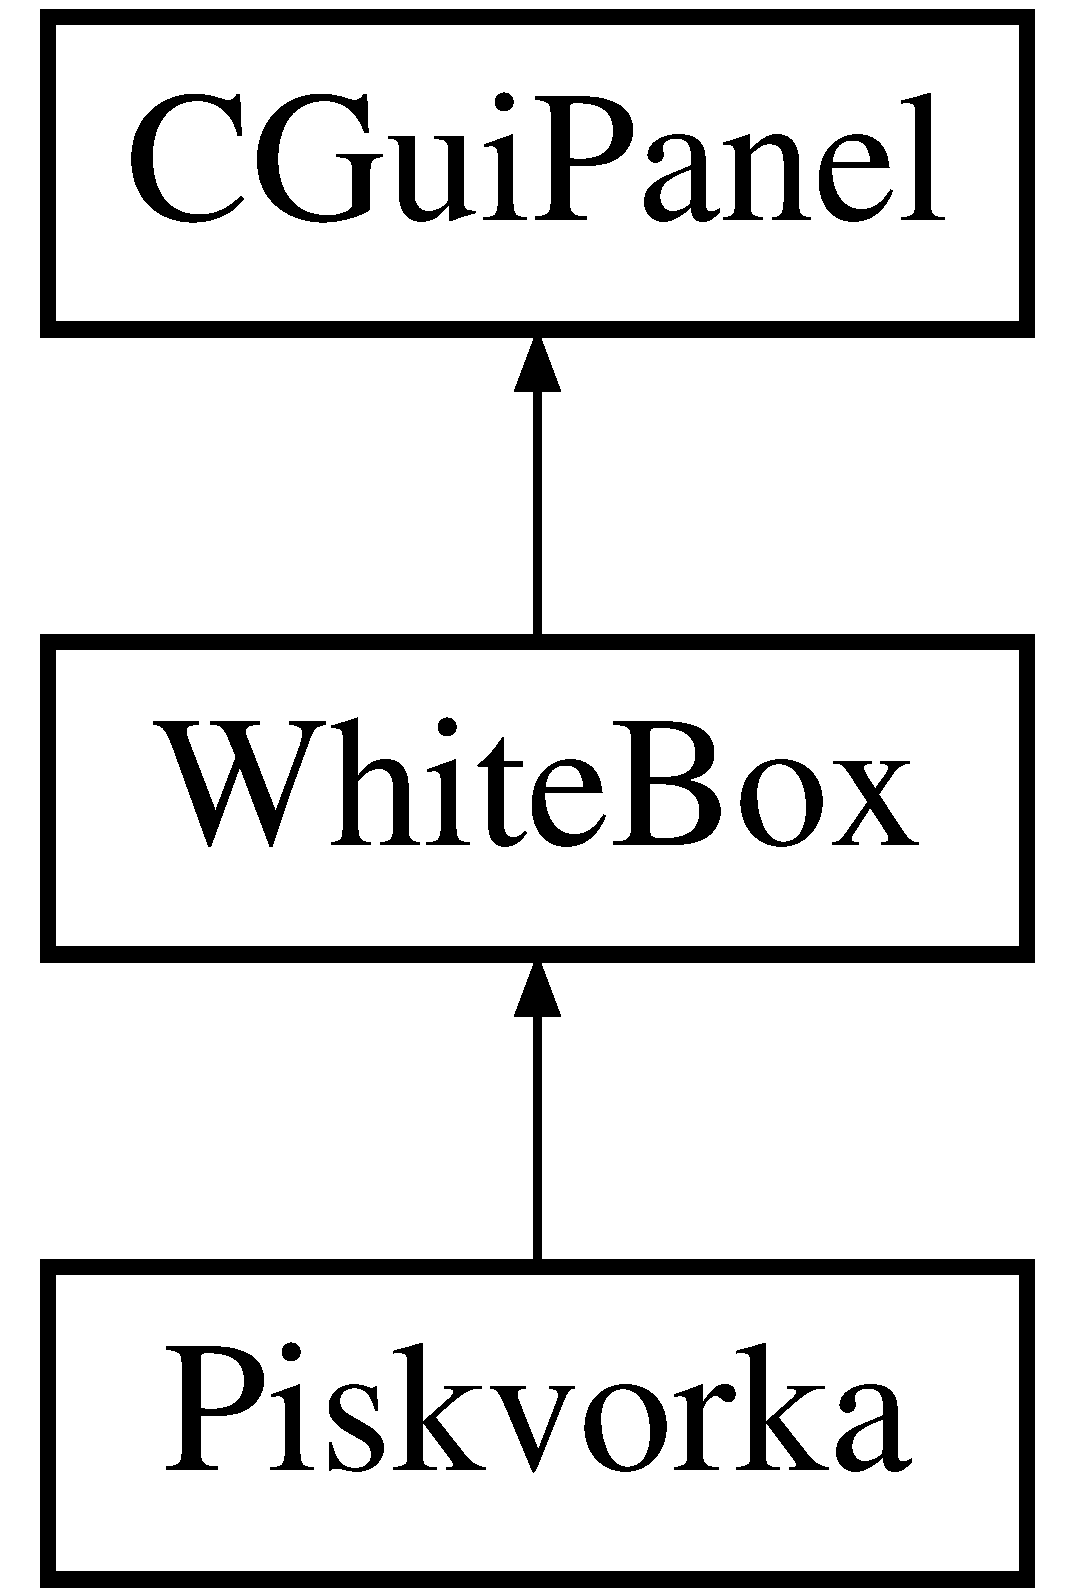
\includegraphics[height=3.000000cm]{class_white_box}
\end{center}
\end{figure}
\subsection*{Public Member Functions}
\begin{DoxyCompactItemize}
\item 
\hypertarget{class_white_box_a01a05b1ae0a0227853a25335a954a8b1}{
{\bfseries WhiteBox} (double x, double y, double w, double h)}
\label{class_white_box_a01a05b1ae0a0227853a25335a954a8b1}

\item 
\hypertarget{class_white_box_a9a94fd76db8e966603ed2a7ede4173f8}{
void {\bfseries draw} ()}
\label{class_white_box_a9a94fd76db8e966603ed2a7ede4173f8}

\item 
\hypertarget{class_white_box_ae582c8cc991d496c834fba16d3ed7385}{
bool {\bfseries onClick} (const \hyperlink{classvec2d}{vec2d} \&position, MouseButton button)}
\label{class_white_box_ae582c8cc991d496c834fba16d3ed7385}

\end{DoxyCompactItemize}
\subsection*{Public Attributes}
\begin{DoxyCompactItemize}
\item 
\hypertarget{class_white_box_a48cbf215391d283595500e9b5f87f556}{
\hyperlink{classrgba}{rgba} {\bfseries color}}
\label{class_white_box_a48cbf215391d283595500e9b5f87f556}

\item 
\hypertarget{class_white_box_a8df6f666921b4f8e0c20e87df6546b35}{
bool {\bfseries isWhite}}
\label{class_white_box_a8df6f666921b4f8e0c20e87df6546b35}

\end{DoxyCompactItemize}


The documentation for this class was generated from the following files:\begin{DoxyCompactItemize}
\item 
src/WhiteBox.h\item 
src/WhiteBox.cpp\end{DoxyCompactItemize}

\hypertarget{class_wrong_parameter_type}{
\section{WrongParameterType Class Reference}
\label{class_wrong_parameter_type}\index{WrongParameterType@{WrongParameterType}}
}
\subsection*{Public Member Functions}
\begin{DoxyCompactItemize}
\item 
\hypertarget{class_wrong_parameter_type_ad0b10b3d7090e80bb2569677bdcdd6b7}{
{\bfseries WrongParameterType} (std::string prm, std::string readType)}
\label{class_wrong_parameter_type_ad0b10b3d7090e80bb2569677bdcdd6b7}

\end{DoxyCompactItemize}


The documentation for this class was generated from the following files:\begin{DoxyCompactItemize}
\item 
src/exceptions.h\item 
src/exceptions.cpp\end{DoxyCompactItemize}

\printindex
\end{document}
